% !TeX program = xelatex
% ================================================================
% 《调和分析中的至上主义》(Suprematism in Harmonic Analysis, 2024,
% Antonio Córdoba) 中文译本 —— 基于数译(mathtranslations.org)排版模板 mathtranslation.cls
% 使用 XeLaTeX 编译两次以上(生成目录、交叉引用、术语索引页码),
% 并用 biber 处理参考文献.
% 依赖: logo.pdf, chapters/*.tex, references.bib, figs/
%
% 编号体系(与原书一致):
%  - 定理类环境(定义/引理/定理/推论/命题/注)共享同一计数器,
%    按"章.序号"编号(如 定理 5.8);
%  - 公式按"章.序号"编号(如 (8.2));
%  - 小节编号 章.节(如 5.7), 小小节 编号 章.节.小节(如 5.7.3);
%  - 参考文献沿用原书全局编号 1–226(主文献 1–17, 其后按章分组).
% ================================================================

\documentclass[
  BookTitleCN={调和分析中的至上主义},
  BookTitleEN={Suprematism in Harmonic Analysis},
  OriginalAuthor={Antonio Córdoba},
  OriginalEdition={Progress in Mathematics Vol. 356},
  OriginalPublisher={Birkhäuser · Springer},
  OriginalYear={2024},
  Translator={数译},
  ModelUsed={GLM-5.3},
  TranslationDate={23 Aug 2026},
  BibStyle=numeric-comp
]{mathtranslation}

% 类文件未含 esint(正文用其积分号)
\usepackage{esint}

% 参考文献数据源(类文件只载入 biblatex, 由文档指定 .bib)
\addbibresource{references.bib}

% 对齐旧版的 biblatex 选项: 作者全名、至多 6 位后 et al.,
% defernumbers 支持按章分组的全局连续编号 1–226.
\ExecuteBibliographyOptions{
  maxbibnames=6,giveninits=false,defernumbers=true,
  isbn=false,url=false,doi=false,eprint=false}

% ================================================================
% 定理类环境
% ----------------------------------------------------------------
% 原书"定义/引理/定理/推论/命题/注/问题/猜想/事实/例"共享同一计数器,
% 按"章.序号"编号(如 定理 5.8). 类文件为每类各建独立计数器, 故先撤销
% 类文件中的定义, 再按共享计数器重建.
% ================================================================
\makeatletter
\def\MT@undefthm#1{%
  \expandafter\let\csname #1\endcsname\relax
  \expandafter\let\csname end#1\endcsname\relax
  \expandafter\let\csname c@#1\endcsname\relax
}
\MT@undefthm{theorem}\MT@undefthm{definition}\MT@undefthm{lemma}%
\MT@undefthm{corollary}\MT@undefthm{proposition}\MT@undefthm{remark}%
\MT@undefthm{example}\MT@undefthm{problem}
\makeatother

% 类文件为上述计数器都注册了 \@addtoreset{...}{section}. 在原书里 section 就是
% "章"(旧模板把章伪装成 section), 故每章重置一次; 重映射到 chapter 之后, section
% 变成"小节", 若不去掉这些钩子, 每进入一个小节定理编号就会被重置.
% 注意: 只能逐个 \@removefromreset, 不能清空整个 \cl@section —— 其中还有
% subsection 的按节重置(book 类原生), 一起清掉会让小节编号不再随节归零.
\makeatletter
\@removefromreset{theorem}{section}
\@removefromreset{definition}{section}
\@removefromreset{lemma}{section}
\@removefromreset{corollary}{section}
\@removefromreset{proposition}{section}
\@removefromreset{remark}{section}
\@removefromreset{example}{section}
\@removefromreset{problem}{section}
\makeatother

% 注: \newtheorem{X}[theorem]{...} 不会为 X 建立计数器, 只把 \theX 指向 \thetheorem.
% 但 hyperref / cleveref 会访问 \the\c@X, 若 \c@X 残留 \relax 便报
% "You can't use \relax after \the". 故重建之后把各别名的计数器寄存器
% 一律指到 theorem 的寄存器上 —— 这正是"共享计数器"的语义.

\theoremstyle{mtfang}
\newtheorem{theorem}{定理}[chapter]
\newtheorem{definition}[theorem]{定义}
\newtheorem{lemma}[theorem]{引理}
\newtheorem{corollary}[theorem]{推论}
\newtheorem{proposition}[theorem]{命题}
\newtheorem{remark}[theorem]{注}
\newtheorem{question}[theorem]{问题}
\newtheorem{conjecture}[theorem]{猜想}
\newtheorem{fact}[theorem]{事实}

\theoremstyle{mtsong}
\newtheorem{example}[theorem]{例}
\newtheorem{problem}[theorem]{问题}

% 无编号版本
\theoremstyle{mtfang}
\newtheorem*{theorem*}{定理}
\newtheorem*{definition*}{定义}
\newtheorem*{lemma*}{引理}
\newtheorem*{corollary*}{推论}
\newtheorem*{proposition*}{命题}
\newtheorem*{remark*}{注}
\newtheorem*{question*}{问题}
\newtheorem*{conjecture*}{猜想}
\newtheorem*{fact*}{事实}
\newtheorem*{claim*}{断言}
\theoremstyle{mtsong}
\newtheorem*{example*}{例}

% 把共享计数器的别名寄存器指到 theorem(见上文的说明)
\makeatletter
\let\c@definition\c@theorem
\let\c@lemma\c@theorem
\let\c@corollary\c@theorem
\let\c@proposition\c@theorem
\let\c@remark\c@theorem
\let\c@question\c@theorem
\let\c@conjecture\c@theorem
\let\c@fact\c@theorem
\let\c@example\c@theorem
\let\c@problem\c@theorem
\makeatother

% 类文件只给 example/remark 挂了菱形结束标记; 与原书一致, 无编号的 remark*
% 不再额外补挂(原模板亦未给 remark* 挂标记)。

% 按类型区分的引用命令
\newcommand{\thmref}[1]{定理~\ref{#1}}
\newcommand{\lemref}[1]{引理~\ref{#1}}
\newcommand{\defref}[1]{定义~\ref{#1}}
\newcommand{\propref}[1]{命题~\ref{#1}}
\newcommand{\corref}[1]{推论~\ref{#1}}
\newcommand{\remref}[1]{注~\ref{#1}}
\newcommand{\exref}[1]{例~\ref{#1}}
\newcommand{\probref}[1]{问题~\ref{#1}}
\newcommand{\quesref}[1]{问题~\ref{#1}}
\newcommand{\conjref}[1]{猜想~\ref{#1}}
\newcommand{\factref}[1]{事实~\ref{#1}}

% ---------- 公式与图: 按"章.序号"编号 ----------
\numberwithin{equation}{chapter}
\counterwithin{figure}{chapter}
\renewcommand{\thefigure}{\arabic{chapter}.\arabic{figure}}

% ================================================================
% 术语索引
% ----------------------------------------------------------------
% 类文件的 \printterminology 假定文档用了 \appendix, 于是"术语索引"
% 会被编成附录章节. 本文献无附录, 若照搬会变成普通的"第 N 章".
% 这里改为无编号章, 与"译者说明""参考文献"一致.
% ================================================================
\let\MTSupOrigChapter\chapter
\newcommand{\MTSupStarChapter}[1]{%
  \MTSupOrigChapter*{#1}%
  \phantomsection\addcontentsline{toc}{chapter}{#1}%
}
\let\MTSupOrigPrintTerminology\printterminology
\renewcommand{\printterminology}{%
  \begingroup
  \let\chapter\MTSupStarChapter
  \MTSupOrigPrintTerminology
  \endgroup
}

% ================================================================
% 常用数学宏
% ================================================================
\newcommand{\R}{\mathbb{R}}
\newcommand{\C}{\mathbb{C}}
\newcommand{\N}{\mathbb{N}}
\newcommand{\Z}{\mathbb{Z}}
\newcommand{\T}{\mathbb{T}}
\newcommand{\Q}{\mathbb{Q}}
\DeclareMathOperator{\supp}{supp}
\DeclareMathOperator{\dist}{dist}
\DeclareMathOperator{\diam}{diam}
\DeclareMathOperator{\mes}{mes}
\DeclareMathOperator{\vol}{vol}
\DeclareMathOperator{\length}{length}
\DeclareMathOperator{\lcm}{lcm}
\DeclareMathOperator{\card}{card}

% 章首题记与图片占位
\newcommand{\epigraph}[2]{%
  \par\vspace{0.8em}
  \begin{flushright}
  \begin{minipage}{0.66\textwidth}
    \raggedleft\itshape #1\par
    \if\relax\detokenize{#2}\relax\else
      \smallskip
      \raggedleft\small——~#2\par
    \fi
  \end{minipage}
  \end{flushright}
  \vspace{0.8em}
}

\newcommand{\FIGPLACEHOLDER}[1]{%
  \fbox{\parbox[c][4cm][c]{0.8\textwidth}{\centering\large [待插入图片: #1]}}%
}

\begin{document}

\makecover

% ---------- 前置部分(罗马页码): 获奖说明、译者说明、目录 ----------
\frontmatter

\thispagestyle{plain}

\begin{center}
  \vspace*{1.5cm}
  {\Large\bfseries 本书荣获 2024 年度 Ferran Sunyer i Balaguer 奖}\\[1.2cm]
\end{center}

\noindent
Ferran Sunyer i Balaguer (1912--1967) 是一位自学成才的加泰罗尼亚数学家.
尽管身患严重残疾, 他在经典数学分析领域的研究一直十分活跃, 并因此在国际上享有声誉.
他的继承人在加泰罗尼亚研究所 (Institut d'Estudis Catalans) 内设立了 Ferran Sunyer i Balaguer 基金会,
以纪念 Ferran Sunyer i Balaguer, 并促进数学研究.

\smallskip
\noindent
基金会每年与加泰罗尼亚研究所共同颁发一项国际研究奖, 授予一部具有综述性质的教学专著.
获奖专著在本丛书中出版. 关于此奖项与基金会的详细信息见
\url{https://ffsb.espais.iec.cat/en/the-ferran-sunyer-i-balaguer-prize/}.

\smallskip
\noindent
2024 年度奖项科学委员会成员:
Ruth Kellerhals (Université de Fribourg),
Jiang-Hua Lu (University of Hong Kong),
Marta Sanz-Solé (Universitat de Barcelona),
Kristian Seip (NTNU),
Yuri Tschinkel (Courant Institute of Mathematical Sciences, New York University).

\chapter*{译者说明}
\addcontentsline{toc}{chapter}{译者说明}

本译本依据 Antonio Córdoba 著 \emph{Suprematism in Harmonic Analysis}
(Birkhäuser, Progress in Mathematics Vol. 356, 2024, Ferran Sunyer i Balaguer 奖 2024 年度获奖著作)译出.
翻译以数学正确性优先, 章节结构、定理编号与公式编号均与原书一致;
正文中的文献引用编号~[n] 亦与原书全局编号一致, 对应关系见文末参考文献.

\vspace{0.5cm}
\hfill \Translator

\hfill \TranslationDate

\tableofcontents

% ---------- 正文(阿拉伯页码) ----------
\mainmatter

% ================================================================
%  前言 (Preface) 与 记号与术语 (Notation and terminology)
%  依据原书 PDF 第 vii--xix 页译出
% ================================================================

\chapter*{前言}
\addcontentsline{toc}{chapter}{前言}

\epigraph{一点小小的帮助，\\来自我的朋友们。}{}

\section*{定理之间的艺术}

新造型主义（Neoplasticism）——其最著名的代表是 Piet Mondrian——与\newterm{suprematism}{至上主义}{suprematism}——Kazimir Malévich 是其最纯粹的诠释者——是两种抽象绘画风格，它们常常出现在实变函数与\newterm{harmonic-analysis}{调和分析}{harmonic analysis}研究文献的图形与插图之中.

尽管彼此不同，这两种风格都主张简单形式的重要性，例如 Mondrian 笔下各边平行于画布坐标轴的矩形，或是 Malévich 笔下具有任意方向的矩形，并且都在构图中使用原色.

一个典型的例子是 Calderón--Zygmund 算法. 给定定义在平面矩形 $R$ 上的非负可积函数 $f$，以及一个严格大于其平均值的固定数 $m$，即 $m > f_R = \frac{1}{\mu(R)} \int_R f$，我们把 $R$ 二进地分成四个矩形，并保留其中 $f$ 的平均值大于 $m$ 的那些. 接着，我们把其余的矩形同样进行二进细分，并沿用同样的准则，保留那些相应平均值大于 $m$ 的矩形，如此继续下去. 在过程结束时，我们将得到包含于原来 $R$ 的一列矩形 $R_j$，它们满足性质 $m < f_{R_j} \le 4m$；并且由 Lebesgue 微分定理，在它们的并集之外几乎处处有 $f(x) \le m$.

如果我们把属于同一代（即边长相同）的序列成员涂上相同的颜色（红、蓝、黄、黑，……），结果看上去就会像一幅 Mondrian 的画. 而由参数 $m$ 的不同值得到的一系列 ``Mondrian 画'' 将为我们提供关于作用在函数 $f$ 上的奇异积分算子之性状的关键信息.

\begin{center}
  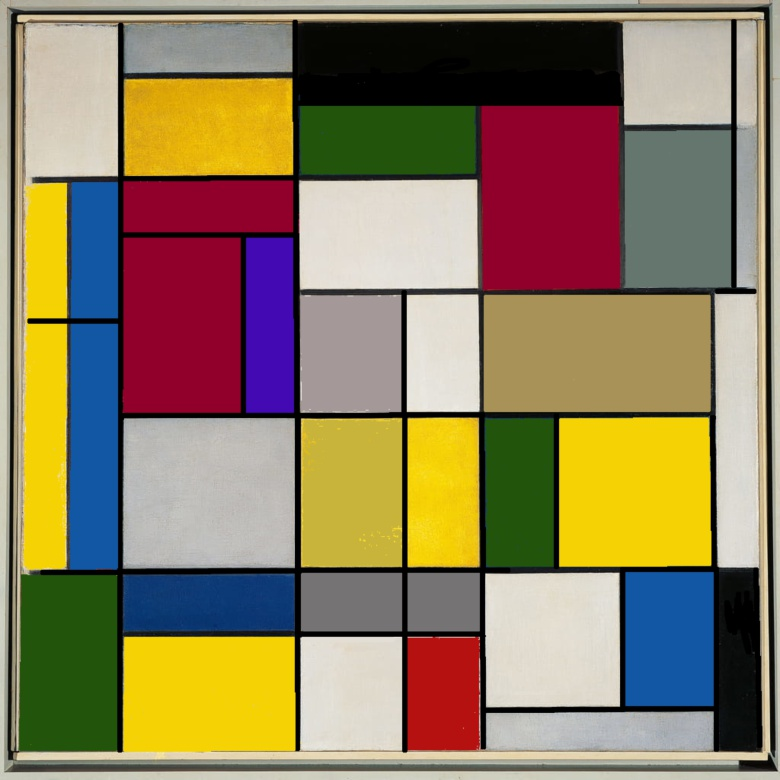
\includegraphics[width=0.55\textwidth]{figs/preface-mondrian.jpeg}

  \smallskip
  {\small\itshape Piet Mondrian 风格的新造型主义绘画.}
\end{center}

\smallskip
然而，调和分析中还有另一些重要的算子，它们涉及欧氏空间中许多方向上的希尔伯特变换，对它们的理解要求按这些不同方向作矩形分解（第 5 章考虑的所谓圆盘乘子便是一个好例子）. 在这些情形中，所得的图像会更像 Malévich 至上主义的构图.

\begin{center}
  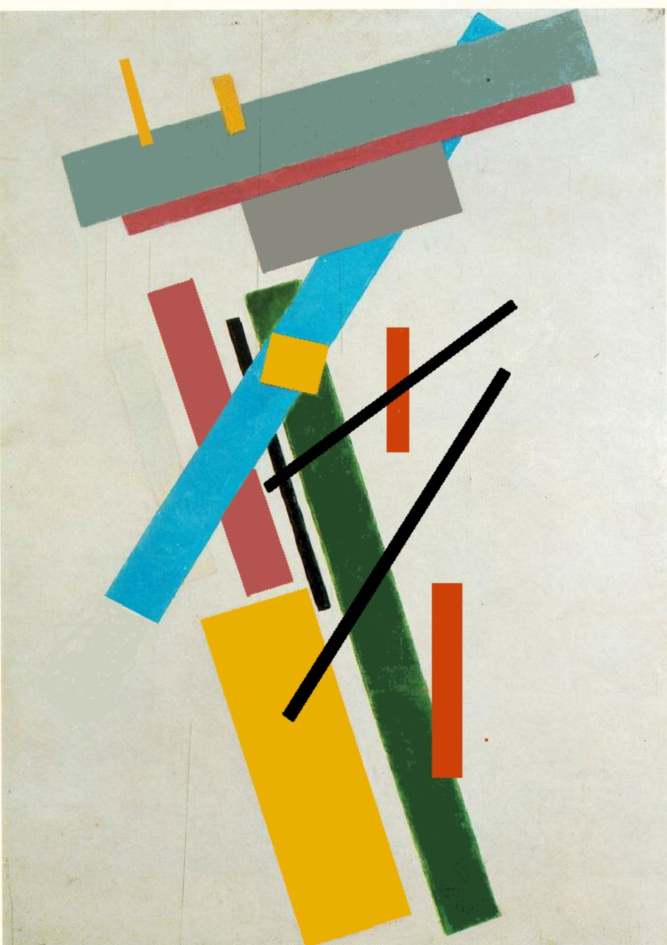
\includegraphics[width=0.4\textwidth]{figs/preface-malevich.jpeg}

  \smallskip
  {\small\itshape 效法 Kazimir Malévich 至上主义的构图.}
\end{center}

\smallskip
我希望这些幼稚的离题之谈有助于为本书的书名辩护——至少是为书名的前半部分，因为后半部分（第 5 至 9 章）并不那么容易纳入这样的比喻；在那里，振荡积分（驻相、Fresnel 衍射、高斯和、van der Corput 估计、Cornu 螺线等）的盛行会让人联想到别样的绘画风格. 大胆一点说，可以把它们与 Vincent van Gogh 的名作《星月夜》联系起来，正如 2009 年 6 月在马德里召开的一次分析学会议的海报所做的那样: 在那幅画中融入了第 5 章二维 Bochner--Riesz 猜想证明中的若干至上主义元素.

\begin{center}
  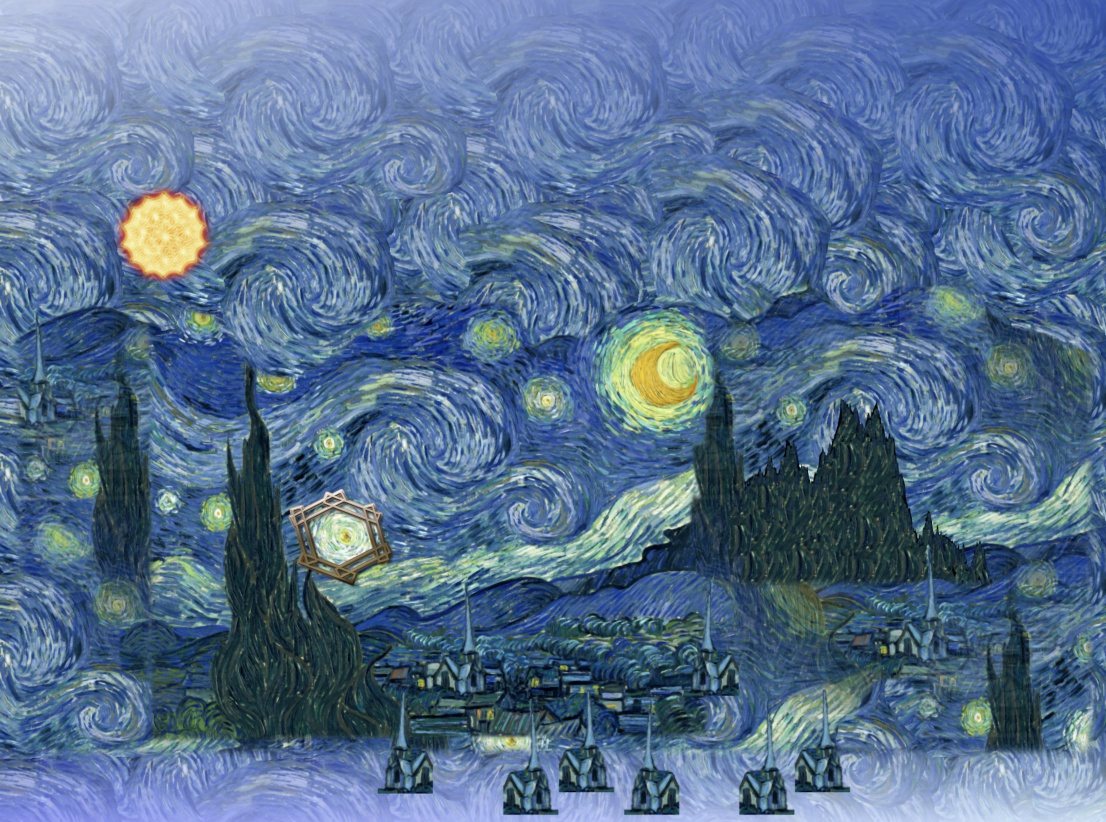
\includegraphics[width=0.62\textwidth]{figs/preface-starrynight.jpeg}

  \smallskip
  {\small\itshape Fernando Chamizo 在 Van Gogh《星月夜》上的至上主义介入.}
\end{center}

\section*{本书的核心}

第 1 章可以看作一首嬉游曲. 让我们把\termcn{数学俳句}定义为这样的陈述: 其表述不需要复杂的术语，其证明锋利而简短，只要掌握了恰当的视角，无须花费太大力气便能理解. 所选的这些俳句中有一些在后续章节中有应用，例如关于凸集的 Fritz John 引理（它使我们可以把由凸集构成的基之微分性质的分析化归为平行多面体的情形），但另一些的入选仅仅是因为我喜欢它们.

第 2 章的背景是经典的 Vitali 覆盖引理，它对欧氏空间中的方体或球成立，而对其他微分基一般不成立；同时还有集族覆盖性质与相应极大算子弱型估计之间的关系. 一个标准的线性化把非线性极大函数的有界性化归为一族线性算子的一致有界性，取它们的伴随（对偶）算子，我们就能用这些伴随所蕴含的覆盖性质来读出弱型不等式.

本章还处理指数型覆盖（它为各边平行于坐标轴的平行多面体所满足），以及 Antoni Zygmund 关于三维欧氏空间中的单调平行多面体族的一个猜想的肯定回答. 本章还有针对带缺项方向的平行多面体所对应极大函数的至上主义式处理.

第 3 章主要讨论 Kakeya 集或 Besicovitch 集的理论，即测度为零、在空间每个方向上都包含一条单位直线段的紧集. 考虑 $\R^n$ 中由离心率（高/半径，或高/底方体边长）等于 $1/\delta$ 的柱体（或平行多面体）构成的族 $\mathcal{B}_\delta$，$0 < \delta < 1$. 给定局部可积函数 $f$，定义
\begin{align*}
  M_\delta f(x) = \sup_{x \in R \in \mathcal{B}_\delta} \frac{1}{\mu(R)} \int_R |f(y)| \, \mathrm{d}\mu(y).
\end{align*}
关于这个极大函数有一个猜想:

\begin{conjecture*}
对每个 $n \ge 2$，存在常数 $C(n)$ 与 $a(n)$，使得对每个 $\delta > 0$，下列估计成立:
\begin{align*}
  \|M_\delta f\|_n \le C(n) \, [1 + |\log \delta|]^{a(n)} \, \|f\|_n.
\end{align*}
\end{conjecture*}

下面是第 3 章的主要结果.

\begin{theorem*}[Kakeya 极大函数定理]
上述猜想在维数 $n=2$ 时成立.
\end{theorem*}

这个定理的一个直接推论是: 二维的每个 Kakeya 集必有等于 $2$ 的 Minkowski 维数（计盒维数），再加一些额外的论证，它也蕴含对 Hausdorff 维数同样的结论. 它的证明可追溯到 1972 年，其概要版 \cite{b41} 于 1975 年刊于 Bulletin of the AMS. C.~Fefferman 在 1974 年温哥华国际数学家大会上题为 ``Recent progress in classical Fourier analysis'' 的大会报告中引用了它. 含有详细证明的论文在同一年（1974 年）被 American Journal of Mathematics 接受，但因积压过多，迟至 1977 年才刊出，见 \cite{b65}. 近来若干作者撰写了关于 Kakeya 集的结果年表，把这一定理的日期记为 1977 年；而严格地说，它在早五年时便已获得，并于 1974 年宣布. 它是我在芝加哥大学博士论文的一部分. 很自然地，我被鼓励去尝试高维的情形，但结果表明这是一项非常艰巨的任务，时至今日仍是一个富有挑战性的公开问题.

尽管如此，有一点是清楚的: 它的解决将由一个恰当的高维覆盖引理所蕴含，而为此自然可以先得到若干特殊情形，它们在如今的文献中以``丛''（bush）与``刷''（brush）构型这样形象的名字著称，即所涉及的柱体（或平行多面体）共享一个公共点（丛），或都与其中某个给定者相交（刷）. 对于这两种构型（丛或刷），都有简单的几何论证给出重叠函数的正确估计，但在当时（1974 年），这些观察被认为不够格单独发表. 多年之后，Jean Bourgain 与 Tom Wolff 重新发现了这些粗针特殊构型的性质，并利用它们得到了维数大于 $2$ 的 Kakeya 集分形维数的下界.

雄心一点，我们可以把下述``至上主义覆盖引理''表述为一个猜想:

\begin{definition*}
平行多面体的有限族 $\{R_i\}$ 具有\termcn{稀疏性}（P），若对每个 $j$,
\begin{align*}
  \mu\Big( R_j \setminus \bigcup_{k \ne j} R_k \Big) \le c \, \mu(R_j),
\end{align*}
其中 $c < 1$ 是一个固定的正常数.
\end{definition*}

\begin{definition*}
平行多面体的有限族 $\{R_\alpha\}$ 称为一个\termcn{丛}（bush），如果它们有非空的交，且该族满足性质（P）.
\end{definition*}

\begin{conjecture*}[至上主义覆盖引理]
给定 $\R^n$ 中平行多面体的族 $\mathcal{B}$，有
\begin{align*}
  \sup_{\substack{\{R_j\} \subset \mathcal{B} \text{ 满足\,(P)} }}
  \frac{1}{\mu(\bigcup_j R_j)} \Big\| \sum_j R_j \Big\|_p
  \;\le\; C_p
  \sup_{\substack{\{R_\alpha\} \subset \mathcal{B} \text{ 是丛} }}
  \frac{1}{\mu(\bigcup_\alpha R_\alpha)} \Big\| \sum_\alpha R_\alpha \Big\|_p,
\end{align*}
这里我们滥用记号，用 $R = R(x)$ 表示集合 $R$ 的示性函数.
\end{conjecture*}

第 4 章讨论傅里叶变换的乘子，着重强调奇异积分加权不等式的角色，循着 Benjamin Muckenhoup \cite{b94} 以及 Ronald Coifman 与 Charles Fefferman \cite{b82} 的开创性工作. 1974 年初，在与 C.~Fefferman 合作、1976 年发表的一项工作（见 \cite{b84}）中，人们观察到: 给定 $\R^n$ 中任意局部可积函数 $f$ 与实数 $r > 1$，则 $M(f^r(x))^{1/r}$——其中 $M$ 表示 Hardy--Littlewood 极大函数——是一个 $A_1$ 类中的权重，且界与函数 $f$ 无关. 这一观察对第 5 章二维 Bochner--Riesz 算子猜想的至上主义式证明是至关重要的，它使那些算子可以用 Kakeya 极大函数来估计. 我为这一方法之美所折服，常在我的报告里断言: 直接的 $L^p$ 不等式并非问题的要害，更好的策略是去寻找带适当权重的 $L^2$ 估计.

在 1976--77 学年，Eli Stein 请我在普林斯顿大学讲授他的调和分析研究生课程，内容是当时关于奇异积分加权不等式的最新结果. 对我而言，这是整理这部分材料的好机会，也极具挑战性，因为 Carl Herz、Alex Nagel、Alice Chang 与 José Luis Rubio de Francia 那一年正在普林斯顿数学系访问，并出席了我的讲课. 那些讲义的笔记后来又用于 1978 年夏在 El Escorial 举行的调和分析会议上所授的短课，并收入其会议录. 我相信它们影响了后来 García-Cuerva 与 Rubio de Francia \cite{b4} 以及 Stein \cite{b13} 对这一主题的表述. 第 4 章可以视为它们的一个更新版本.

第 5 章从 C.~Fefferman 对圆盘乘子猜想的反例开始，其中用到了 Kakeya 集的性质，这一反例正是本书所强调的研究进路的源头. 接着是二维 Bochner--Riesz 算子的有界性；对这一结果，文献中另有两种证明，分别由 Lennart Carleson 与 Per Sjölin \cite{b103} 以及 Lars Hörmander \cite{b117} 给出，但其所用方法不同于这里采用的至上主义观点.

与 Kakeya 极大定理一起，我们的证明还涉及若干平方函数估计. 其中一些已知在一般维数成立: 设 $\mathcal{L} = \{R_\nu\}$ 是 $\R^n$ 中内部两两不交的全等平行多面体构成的格，考虑由公式 $\widehat{P_\nu f}(\xi) = R_\nu(\xi) \widehat{f}(\xi)$ 定义的傅里叶乘子 $P_\nu$. 定义平方函数 $G(f) = \big( \sum_\nu |P_\nu(f)|^2 \big)^{1/2}$. 则下列不等式成立:
\begin{align*}
  \int_{\R^n} |Gf(x)|^2 \, w(x) \, \mathrm{d}x \ \lesssim_r \
  \int_{\R^n} |f(x)|^2 \, [M_s w^r(x)]^{1/r} \, \mathrm{d}x,
\end{align*}
其中 $r > 1$，$M_s$ 表示强极大函数，而 $f$ 与 $w > 0$ 是任意的函数: $f$ 属于 Schwartz 类，$w$ 局部可积.

但还有另一些平方函数，其确切的有界性只在二维已知. 给定 $\delta < 1$，定义一个 $\delta$-板（plate）为高 $\delta$、半径 $\delta^{1/2}$ 的柱体. 设 $\{B_j\}$ 是与单位球面相切的两两不交的 $\delta$-板族，且对每个 $j$，$f_j$ 是傅里叶变换支于 $B_j$ 的光滑函数.

\begin{conjecture*}[至上主义平方函数引理]
成立估计
\begin{align*}
  \Big\| \sum_j f_j \Big\|_{2n/(n-1)} \ \lesssim \
  \Big\| \Big( \sum_j |f_j|^2 \Big)^{1/2} \Big\|_{2n/(n-1)},
\end{align*}
其中的常数与 $\delta$ 无关.
\end{conjecture*}
当 $n = 2$ 时指数 $2n/(n-1)$ 恰为 $4$，这对该猜想的二维证明大有助益；而在高维，它仍然是公开的.

可以说，二维的理论如今已被充分理解，本章试图对其主要面貌作一个相当完整的陈述，包括傅里叶变换在圆周上的限制、角平方函数的估计、Bochner--Riesz 平均的几乎处处收敛，以及沿平面曲线的希尔伯特变换的 $L^p$ 估计.

第 6 章是对第 5 章的补充，对关于球乘子的那个被否证的猜想给出了一个肯定的回答: 若把 $L^p(\R^n)$（$\frac{2n}{n+1} < p < \frac{2n}{n-1}$）换成 $L^p_{\mathrm{rad}} L^2_{\mathrm{ang}}(\R^n)$，则猜想成立，球乘子算子在这一档混合范数空间上有界. 在角向部分取 $L^2$ 范数有助于击败 Kakeya 集这个对手，从而建立起一个定理. 证明的方法如今有所不同，依赖于任意阶贝塞尔函数的十分精确的渐近公式. 这一研究进路受到信号理论中带限函数研究的影响，特别是长球面波函数级数的收敛性，以及 Dirichlet 边界条件下单位球上拉普拉斯算子本征函数级数的展开理论.

第 7 章讨论泊松求和公式，它可以用一个格 $\mathcal{L}$ 及其对偶格 $\mathcal{L}^*$ 来表述: 由置于 $\mathcal{L}$ 的顶点处的 $\delta$ 函数之和给出的缓增分布，其傅里叶变换等于支在 $\mathcal{L}^*$ 顶点处的 $\delta$ 函数之和（至多差一个由基本胞腔体积决定的因子）.

除了众多重要的数学应用之外，该公式在晶体学中也很要紧，因为在那里，分子的电子密度函数的傅里叶变换通常与其 X 射线谱相联系，历史上，这一观察曾是理解固体的关键一步. 晶体学范式说: 周期结构产生锐利的 Bragg 峰，而这些峰的分布的知识应能允许我们重建晶体（也许要除去丢失的相位，但那是另一个问题）. X 射线晶体学家们编制出了晶体的目录及其对称群的分类. 但是这座大厦在上世纪八十年代中期遭受了一次地震般的冲击: 准晶体被发现了——那是一些材料，其 X 射线谱呈现清晰的 Bragg 峰，却带有理论所不允许的五重对称性.

1986 年我在苏黎世联邦理工学院（ETH）访问，参加了由 John Garnett 组织的调和分析学期活动，其间我听了好几场关于这一问题的报告. 我的第一反应是追问是否还有别的泊松公式，经过几周的工作，我得到了答案: 没有别的公式了. 更精确地说: 给定两个离散点集 $X = \{x_j\}$ 与 $Y = \{y_k\}$，若缓增分布 $\sum \delta_{x_j}$ 的傅里叶变换等于 $\sum \delta_{y_k}$，则 $X$ 与 $Y$ 必是基本胞腔体积为 $1$ 的互相对偶的格. 这就是第 7 章的开篇定理，它发表 \cite{b154} 于法国科学院的 Comptes Rendus——在此之前，我的几位朋友，全是杰出的调和分析学家，都敦促我发表，因为据他们相告，这个证明对他们而言是新的. 若在早些年，它本可以被视为晶体学的一条基本定理，但准晶体的出现改变了晶体的经典定义，给数学家留下了如下任务: 为理解新材料的 X 射线谱，去研究并分类更一般的泊松求和公式. 依我之见，这项任务还远未完成.

在前几章考虑过 $\R^k$ 中球的傅里叶变换之后，对泊松求和公式的讨论不可避免地把我们引向数论中的格点问题，即估计以原点为中心、$r$ 为半径的球内格点数时，用球的体积去近似所造成的误差项. 沿 Hardy 的路线，泊松公式使我们能把误差项写成含贝塞尔函数与算术函数 $r_k(m)$ 的解析表达式，其中 $r_k(m)$ 计数把 $m$ 表为 $k$ 个平方和的表法数. 这里无意对如此重要而有趣的理论作公允的综述，只想强调泊松公式在为误差项产生解析可处理的表达式方面的作用. 引 Fernando Chamizo 的话: ``泊松公式容许我们把数格点换成数波''. 与前面各章的 Bochner--Riesz 问题相比，一个显著的差别是: 这里的困难在于二维和三维，而对 $k \ge 4$，由于 $r_k(m)$ 的行为更规则，误差项的确切估计是已知的.

本章还包含把理论推广到平面上凸区域的工作，其精神源自 Feynman 的路径积分，它有助于理解并界定在重要情形 $k=2$ 中关于该误差项的 Hardy 猜想的困难所在. 本章还有若干关于 X 射线谱学中相位恢复问题的杂评，它们与高斯和有关.

调和分析与数论的交界面如此广阔、成果如此丰富，以至于第 8 章只能指望指出其中若干论题——也许不是最重要的，但我希望多少是有意义的. 在那个领域里，Riemann 与 Hardy 的名字无处不在；``圆法''、``Vinogradov 均值定理''或``三角和的 Weyl 估计''等技巧举足轻重；而前面提到过的格点计数、Waring 问题或 Goldbach 猜想等问题，则一直是两个学科之间十分有趣的数学互动的源泉.

为给第 8 章定位，一个合适的起点是 Zygmund 书中研究特殊三角级数的部分. 在那里我们可以找到缺项级数的性质，即形如 $\sum_k a_k \exp(2\pi i n_k x)$、频率几何式增长的级数: $n_{k+1}/n_k > \rho > 1$. 书中证明: 若这样的级数是某个可积函数的\newterm{fourier-series}{傅里叶级数}{Fourier series}，则该函数的任何正幂次也必可积，且相应的 $L^p$ 范数都与其 $L^2$ 范数等价. 如今我们还可以把上述论断精确化: 该级数还属于空间 BMO（有界平均振荡）. Zygmund 这部论著的细心读者会在那一部分发觉缺少了频率按 $k$ 次幂增长时的相应命题. 初步的考虑给出限制 $p < 2k$: 若可积函数的傅里叶级数的频率都是 $k$ 次幂，则该函数必属于 $L^p$. 但 $p < 2k$ 时的这一断言仍是一个突出的困难公开问题，即使在 $k = 2$ 的情形——那里我们对高斯和有非常精确的信息. 当我们把问题用傅里叶级数的乘子算子来重述时，会发现相应的核与第 4 章考虑的奇异积分大不相同. 这里恰可想起 Henryk Iwaniec 的评论: ``在调和分析里，我们是把好核作用于复杂的函数；而在数论里，我们是把难的核作用于非常光滑的函数.''

在本章中，读者会看到关于这一问题的一些观察和特殊情形，但没有它的解. 不过，未能补全 Zygmund 之书的沮丧，可以因如下的发现得到缓解: 三角级数
\begin{align*}
  \sum_{n \ge 1} n^{-(1+\delta)} e^{2\pi i n^k \cdot x}
\end{align*}
的图象的 Minkowski 维数是可以精确计算的，而这些级数在 Riemann 的学位论文 \cite{b194} 中已被考虑过，在那里他还推广了当时通行的积分与导数的概念，除此之外还有别的有趣论题.

本章以数论对傅里叶级数的一种收敛方法的应用作结，其中的部分和如今是按系数的大小来选取的. 由于前一章描述的理由，这是在晶体学中很自然的一种方法.

第 9 章从对原子 Born--Oppenheimer 理论的简快介绍开始，包括对原子序数为 $Z$ 的中性原子的基态的 Thomas--Fermi 与 Hartree--Fock 近似的一种印象派式描述. 其目的在于说明三角和的 Weyl 估计在原子能量振荡中所起的作用，这一现象对从量子力学第一性原理出发理解化学元素周期表具有意义. 这是 C.~Fefferman 与 Luis Seco \cite{b206} 在对大原子基态能量渐近公式的 Dirac--Schwinger 修正作严格处理时发现的一个效应，随后在若干出版物中又被深入分析 \cite{b200,b201,b207,b209,b223}. 本章只打算为认真关心该理论的读者提示进一步的读物，且在某种意义上，它是第 1 章数学俳句思想的对应物. 但它足以传达调和分析的深度与多样性: 从欧氏空间中平行多面体的初等几何开始，到关于原子能量振荡的量子力学问题结束.

幸运的是，经典傅里叶分析有若干杰出的论著，例如 Zygmund 的 \emph{Trigonometric series} \cite{b17}，Stein 的 \emph{Singular integrals and differentiability properties of functions} \cite{b12}，以及 Stein 与 Guido Weiss 的 \emph{Introduction to Fourier analysis on Euclidean spaces} \cite{b14}；我假定读者对它们的内容已有所知. 本书的主要目的是呈现若干超出这些著名专著范围的结果——这一抱负听上去比实际上更为雄心勃勃. 一份更详尽的有益参考文献清单见文末参考文献的开头部分.

\section*{几则个人感言}

有一次，我参加一个报告，报告人在黑板上写下``分析学家 = 猎人''这句话，并如此解释: ``分析学家像猎人一样，把大部分时间花在总部里打磨他的工具. 他有时出去打猎，但很快就回到家中，继续磨快他的刀.''

年龄不是一个特别有趣的话题，但它通常有助于获得某种视角. 上世纪七十年代初，作为芝加哥大学的研究生，我有幸亲眼见证了 Alberto Calderón 与 Antoni Zygmund 学派发展起来的奇异积分理论对线性偏微分方程的成功冲击，它解决并照亮了诸如双曲方程 Cauchy 问题的唯一性、椭圆边值问题、局部可解性的刻画或指标定理等基本问题. 在导师的指点下，我熟读了原始文献，即 Calderón--Zygmund、Kohn--Nirenberg、Beals--Fefferman、Atiyah--Singer 以及其他许多人的著作，这促使我在七十年代末在马德里康普鲁滕塞大学开设了一门研究生课程，其讲义以 \emph{Pseudodifferential operators and applications}（伪微分算子及其应用）为题在当地出版. 在那些年里，发展伪微分算子与傅里叶积分算子的理论，并猎取它们对线性偏微分方程的应用，是傅里叶分析主流的活动. 这场活动也催生了一批综述与专著，并在 Lars Hörmander 那部里程碑式的巨著 \cite{b8} 中达到顶点——我认为它把这一主题封闭了几十年.

主流随后改变了方向，转而注意非线性问题. 五十年代末 E.~de Giorgi 与 J.~Nash 的开创性工作如同一块罗塞塔石碑，使人们得以理解椭圆与抛物型的非线性方程——例如极小曲面所满足的方程——并为处理自由边界问题与相变开辟了道路；在那里，奇异积分理论再次极为有用. 还有 J.~Leray 以及其他许多人对流体力学方程的贡献；在那里，傅里叶分析学家磨快的工具再一次成为关键.

粗略地说，我们可以把这些视为那些年里调和分析学家的主要猎场. 不过也有其他重要的活动领域，例如 J.~von Neumann 与 H.~Weyl 对量子力学的严格数学奠基，或者 Hardy--Littlewood--Ramanujan 对数论的杰出贡献. 但在那里，尤其是在数论中，正如 H.~Iwaniec 指出的，所需估计中涉及的核的性质偏离了 Calderón--Zygmund 范式.

我与多位杰出的合作者一起，在那些主流领域工作并发表过文章. 但我也关心过另一些较为``旁系''的问题，例如前面提到的 Zygmund 关于积分微分的猜想、Kakeya 集与 Bochner--Riesz 求和、推广的泊松求和公式，以及 Riemann 图象的分形维数. 本书主要就是关于这些旁系主题的，它源自 2020 年冬季学期我在穆尔西亚大学讲授的一门研究生课程. 新冠疫情使这门课在随后几年未能继续，但尽管我至今仍不很明白完成这些讲义的理由，我还是力图把我多年的想法有条理地呈现出来，或许带着一点夸张的自负: 某些读者也许能从中找到未来研究的灵感.

\section*{致谢}

我怀着极大的愉快向所有尊敬的研究合作者致谢，他们的贡献丰富了本书的内容. 我要特别感谢 Pablo Fernández Gallardo 与 Fernando Chamizo，他们宝贵的洞见与建议对提升本书的表述质量与协调各章内容起到了关键作用.

我还要对穆尔西亚大学表示感谢，奠定本书基础的研究生课程正是在那里讲授的；同时感谢数学科学研究所（ICMAT）的 Severo Ochoa 项目慷慨的经费资助.

最后，我感激 Alfonso Núñez 与 Irene Quintero 出色的专业技艺，他们把我最初的手写稿转化为规范的 LaTeX 格式，使之得以面向更广的读者.

\begin{flushright}
  马德里，2024 年 8 月

  \medskip
  Antonio Córdoba
\end{flushright}

\vspace{1cm}

% ================================================================
%                        记号与术语
% ================================================================

\chapter*{记号与术语}
\addcontentsline{toc}{chapter}{记号与术语}

\begin{itemize}
\item
  $\chi_A$ 是集合 $A$ 的示性函数的标准记号. 为了简化记号，在不致混淆时，将简写为 $A(x) = \chi_A(x)$:
  \begin{align*}
    A(x) = \chi_A(x) =
    \begin{cases}
      1, & \text{若 } x \in A, \\
      0, & \text{若 } x \notin A.
    \end{cases}
  \end{align*}

\item
  给定定义在区域 $D$ 上的两个实函数 $f$ 与 $g$，记号 $f \lesssim g$ 表示存在有限正常数 $C$，使得对每个 $x \in D$ 都有 $f(x) \le C g(x)$. 类似地，$f \gtrsim g$ 表示对 $x \in D$ 有 $f(x) \ge C g(x)$. 而 $f \simeq g$ 表示 $f \lesssim g$ 且 $g \gtrsim f$.

  记号 $\ll$、$\gg$ 分别等同于 $\lesssim$ 与 $\gtrsim$. 它们由 I.~Vinogradov 引入，主要用于数论文献；而 $\lesssim$、$\gtrsim$ 与 $\simeq$ 是调和分析中的常用记号.

\item
  $[x]$ 表示 $x$ 的整数部分；$\{x\}$ 表示 $x$ 的小数部分.

\item
  $J_k$ 表示 $k$ 阶第一类贝塞尔函数.

\item
  除非另有明文说明，$\mu(A)$ 表示集合 $A \subset \R^n$ 的\newterm{lebesgue-measure}{Lebesgue 测度}{Lebesgue measure}. 在某些场合也使用记号 $|A| = \mu(A)$.

\item
  我们用 $\fint_R f$ 表示平均值:
  \begin{align*}
    \fint_R f = \frac{1}{\mu(R)} \int_R f(x) \, \mathrm{d}\mu(x).
  \end{align*}

\item
  \newterm{fourier-transform}{傅里叶变换}{Fourier transform}:
  \begin{align*}
    \widehat{f}(\xi) = \int_{\R^n} e^{-2\pi i x \cdot \xi} \, f(x) \, \mathrm{d}x.
  \end{align*}

\item
  Mellin 变换:
  \begin{align*}
    M f(s) = \int_0^\infty t^{-is} f(t) \, \frac{\mathrm{d}t}{t}.
  \end{align*}

\item
  \newterm{convolution}{卷积}{convolution}:
  \begin{align*}
    f * g(x) = \int_{\R^n} f(x - y) \, g(y) \, \mathrm{d}y.
  \end{align*}
  记号 $f *_i g$ 表示仅在第 $i$ 个变量上作卷积.

\item
  $M(f)$ 表示 Hardy--Littlewood 极大函数.

\item
  $M_s(f)$ 表示强极大函数.

\item
  $M_N(f)$ 表示 Kakeya 极大函数（离心率为 $N$ 的矩形）.

\item
  主值积分:
  \begin{align*}
    \mathrm{p.v.} \int_{\R^n} g(x) \, \mathrm{d}x
    = \lim_{\varepsilon \to 0^+} \int_{|x| \ge \varepsilon} g(x) \, \mathrm{d}x.
  \end{align*}

\item
  沿方向 $v$ 的希尔伯特变换:
  \begin{align*}
    H_v f(x) = \lim_{\varepsilon \to 0^+} \int_{|t| \ge \varepsilon} \frac{f(x - vt)}{t} \, \mathrm{d}t.
  \end{align*}

\item
  $\mathrm{d}\sigma(\bar{y})$ 是 $\R^n$ 中单位球面 $S^{n-1}$ 上的 Lebesgue 测度.

\item
  $L^p_{\mathrm{rad}} L^2_{\mathrm{ang}}(\R^n)$ 是满足
  \begin{align*}
    \Big[ \int_0^\infty \Big( \int_{S^{n-1}} |f(r\bar{y})|^2 \, \mathrm{d}\sigma(\bar{y}) \Big)^{p/2} r^{n-1} \, \mathrm{d}r \Big]^{1/p} < \infty
  \end{align*}
  的函数 $f$ 所构成的空间.
\end{itemize}
   % 前言与记号说明

% ================================================================
%  第 1 章 七则数学俳句 (Seven mathematical haikus)
%  依据原书 PDF 第 1--19 页译出；编号审计见文件末尾注释
% ================================================================

\chapter{七则数学俳句}

\epigraph{月光之下, \\紫藤的花色与芬芳, \\仿佛都很遥远。}{与谢芜村（Yosa Buson）}

在数学中, 我们常常要付出艰苦的努力才能证明定理；而即便运气好, 遇到的也往往是复杂的证明, 它们也要求可能的读者付出大量的劳动. 为一条出色的数学陈述找到一个聪明而简短的证明, 是难得的成功. 让我们把缪斯的这些珍贵馈赠称为\newterm{mathematical-haiku}{数学俳句}{mathematical haiku}——大多数数学家肯定都珍藏了好几个例子. 下面是我偏爱的几个.

\section{凸集上 Fritz John 引理的一个几何证明}

\begin{theorem}\label{thm:1.1}
设 $K \subset \R^n$ 是内部非空的紧凸集, $E$ 是包含 $K$ 的体积最小的\newterm{ellipsoid}{椭球}{ellipsoid}. 则有包含关系
$\frac{1}{n}E \subset K$
（其中 $\frac{1}{n}E$ 表示由 $E$ 关于其中心以比率 $1/n$ 收缩得到的椭球）.
\end{theorem}

一个有趣的例子是顶点为 $(P_0, P_1, \ldots, P_n)$（其中向量 $P_1 - P_0, \ldots, P_n - P_0$ 线性无关）的 $(n+1)$-单形 $\sum(P_0, P_1, \ldots, P_n)$:
\begin{align*}
  \sum(P_{0},P_{1},\ldots,P_{n})
  =\Big\{P\in\R^{n}\Big|P=\sum_{j=0}^{n} t_{j} P_{j},
  \text{ 其中 } 0\leq t_{0},t_{1},\ldots,t_{n}\leq 1,\ \sum_{j=0}^{n} t_{j}=1\Big\}.
\end{align*}
当 $\dist(P_{j}, P_{k})$ 对所有不同的顶点对都相同时, 称该单形为\newterm{equilateral-simplex}{等边单形}{equilateral simplex}.

在 $\R^n$ 中内接于某个球面的所有 $(n+1)$-单形中, 体积最大者必为等边单形——一个直接的几何论证即可证明这一点. 由此可得: 给定任一 $(n+1)$-单形 $T$, 存在唯一的包含 $T$ 的体积最小椭球 $E$: 这个 $E$ 是把内接于等边 $(n+1)$-单形 $T'$ 的外接球面, 经把 $T'$ 映为 $T$ 的仿射变换所得到的象.

这一事实有一个对偶的说法: 在包含给定等边 $(n+1)$-单形的所有椭球中, 体积最小者是其外接球面.

\begin{proof}
首先注意, 包含 $K$ 的体积最小椭球的存在性由紧性论证容易得到；而且, 如等边 $(n+1)$-单形的情形所示, 收缩因子 $1/n$ 是精确的.

我们用反证法. 假设存在紧\newterm{convex-set}{凸集}{convex set} $K$, 使得 $\frac{1}{n}E$ 不包含于 $K$. 由于仿射变换保持紧的、有界的凸集类以及椭球类, 不失一般性可设 $E$ 是一个球. 取一点 $P \in (\frac{1}{n}E) \cap (\R^n - K)$, 用 $H$ 表示过 $P$ 且不与 $K$ 相交的一张超平面, 即 $K$ 包含在 $H$ 所界定的两个半空间之一（记为 $H^+$）中（见图~\ref{fig:1.1}, 其中 $K$ 包含在 $E$ 的虚线部分之内）.

\begin{figure}[htbp]
\centering
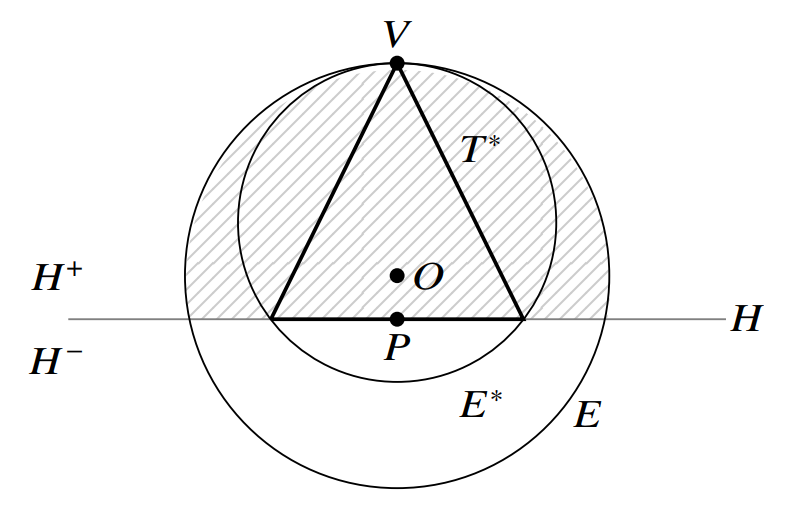
\includegraphics[width=0.5\textwidth]{figs/fig-1-1.png}
\caption{Fritz John 引理.}
\label{fig:1.1}
\end{figure}

作一个等边 $(n+1)$-单形 $T^*$, 使其一个顶点位于 $V$（放在虚线区域 $E \cap H^+$ 的边界与 $E$ 的过 $P$ 的直径的交点处）, 而其余 $n$ 个顶点位于超平面 $H$ 内以 $P$ 为心的 $(n-1)$-球面 $S^*$ 上: $S^* = H \cap E^*$, 其中 $E^*$ 是 $T^*$ 的外接球. 设 $A$ 是保持直线 $OP$ 不动且把 $S^*$ 映为 $S = E \cap H$ 的仿射变换. 那么 $A(E^*)$ 是包含 $A(T^*)$ 的体积最小椭球. 特别地, 有严格不等式 $\vol(E) > \vol(A(E^*))$. 但 $A(E^*) \supseteq E \cap H^+ \supseteq K$, 这与 $E$ 作为包含 $K$ 的体积最小椭球的选取相矛盾.
\end{proof}

Fritz John 给出的\thmref{thm:1.1}的原始证明 \cite{b35} 是不同的, 而且复杂得多. 这条引理在多个理论中扮演重要角色. 例如, 它是把与凸集相联系的极大函数化归为对平行多面体取平均这一特殊情形的恰当工具. 大约 1969 年, 当我还是本科生、在 M.~de Guzmán 的实变函数课上学习时, 应老师之请, 我与同学 A.~Gallego 合作, 为这条有趣的引理寻找一个初等的几何证明. 我们的证明在 1970 年冬于（西班牙）穆尔西亚召开的西班牙数学会会议上作为短篇报告宣读, 后来收录在 \cite{b29,b32} 中. 我相信如今它只被视为凸分析中的一个民间结果, 它曾被多人使用, 其中包括 L.~Caffarelli 在其关于 Monge--Ampère 方程的工作 \cite{b21} 中, 以及 C.~Fefferman 在其 Whitney 扩张结果 \cite{b33} 中.

\section{$\zeta(2)$ 的一个初等计算}

著名的恒等式 $\sum_{n=1}^{\infty}1/n^2 = \pi^2/6$ 最初由 L.~Euler 利用 $\sin(z)/z$ 的无穷乘积展开证明, 但它也可以作为贝塞尔恒等式应用于函数 $y = x$（$0 < x < 1$）的傅里叶系数的推论得到. 如今文献中还可以找到若干别的证明, 它们把 $\zeta(2)$ 的计算化归为适当平面区域上的二重积分；下面我们给出其中一种的细节.

\begin{theorem}\label{thm:1.2}
我们有
\begin{align*}
  \sum_{n=1}^{\infty}\frac{1}{n^{2}}=\frac{\pi^{2}}{6}.
\end{align*}
\end{theorem}

\begin{proof}
写
\begin{align*}
  \zeta(2)=\sum_{n=1}^{\infty}\frac{1}{(2n)^{2}}+\sum_{n=0}^{\infty}\frac{1}{(2n+1)^{2}}.
\end{align*}
即
\begin{align*}
  \zeta(2)
  &=\frac{4}{3}\sum_{n=0}^{\infty}\frac{1}{(2n+1)^{2}}
   =\frac{1}{3}\sum_{n=0}^{\infty}\Big(\int_{-1}^{+1}x^{2n}\,\mathrm{d}x\Big)^{2}
   =\frac{1}{3}\sum_{n=0}^{\infty}\int_{-1}^{+1}\int_{-1}^{+1}(x^{2}y^{2})^{n}\,\mathrm{d}x\,\mathrm{d}y\\
  &=\frac{1}{3}\int_{-1}^{+1}\int_{-1}^{+1}\frac{\mathrm{d}x\,\mathrm{d}y}{1-x^{2}y^{2}}.
\end{align*}
变量替换
\begin{align*}
  x=\tanh(s)=\frac{\exp(s)-\exp(-s)}{\exp(s)+\exp(-s)}, \qquad
  y=\tanh(t)=\frac{\exp(t)-\exp(-t)}{\exp(t)+\exp(-t)}, \qquad
  -\infty<s,\,t<+\infty,
\end{align*}
给出
\begin{align*}
  \zeta(2)=\frac{1}{3}\int_{-\infty}^{\infty}\int_{-\infty}^{\infty}
  \frac{\mathrm{d}s\,\mathrm{d}t}{\cosh(s)^{2}\cosh(t)^{2}-\sinh(s)^{2}\sinh(t)^{2}}.
\end{align*}
但由于双曲函数
\begin{align*}
  \cosh(s)=\frac{\exp(s)+\exp(-s)}{2}, \qquad
  \sinh(s)=\frac{\exp(s)-\exp(-s)}{2}
\end{align*}
满足恒等式
\begin{align*}
  \cosh(s)\cosh(t)-\sinh(s)\sinh(t)=\cosh(s-t),
\end{align*}
\begin{align*}
  \cosh(s)\cosh(t)+\sinh(s)\sinh(t)=\cosh(s+t),
\end{align*}
我们得到
\begin{align*}
  \zeta(2)=\frac{1}{3}\int_{-\infty}^{\infty}\int_{-\infty}^{\infty}
  \frac{\mathrm{d}s\,\mathrm{d}t}{\cosh(s-t)\cosh(s+t)}.
\end{align*}
再作变量替换 $u = s - t$, $v = s + t$, 得
\begin{align*}
  \zeta(2)=\frac{1}{6}\int_{-\infty}^{\infty}\int_{-\infty}^{\infty}
  \frac{\mathrm{d}u\,\mathrm{d}v}{\cosh(u)\cosh(v)}
  =\frac{2}{3}\Big(\int_{0}^{\infty}\frac{\mathrm{d}z}{1+z^{2}}\Big)^{2}
  =\frac{\pi^{2}}{6},
\end{align*}
其中用到了替换 $x = \log z$, $z > 0$.
\end{proof}

\begin{remark}\label{rem:1.3}
如前所述, 这条著名公式有许多不同的证明. Euler 的原始证明的优点是还能给出 $\zeta$ 在一切正偶数 $2k$ 处的值, 但这里给出的证明位居最直接、最简单者之列. 与双曲正切相联系的变量替换的想法是一次奇妙的意外收获: 当时我正在写一篇关于 Ginzburg--Landau 模型中相变的文章, 同时又应西班牙数学会期刊 La Gaceta de la Real Sociedad Matemática Española 的编辑之邀, 撰写一篇综述文章 \cite{b26}, 介绍我对 R.~Apéry 的 $\zeta(3)$ 无理性证明的 1979 年未刊版本. 于是, 在计算 $\zeta(2)$ 与 $\zeta(3)$ 的同时, 图象 $y = \tanh(x/\varepsilon)$ 正作为 $+1$ 与 $-1$ 两态之间相变的例子出现在我的另一项工作中.
\end{remark}

\section{$\zeta(3)$ 的无理性}

公式
\begin{align*}
  \zeta(3)=\sum_{n=1}^{\infty}\frac{1}{n^{3}}
  =-\frac{1}{2}\int_{0}^{1}\int_{0}^{1}\frac{\log(st)}{1-st}\,\mathrm{d}s\,\mathrm{d}t
\end{align*}
由熟知的恒等式
\begin{align*}
  \int_{0}^{1}\int_{0}^{1}\frac{s^{\alpha+\gamma}t^{\alpha+\gamma}}{1-st}\,\mathrm{d}s\,\mathrm{d}t
  =\sum_{n=1}^{\infty}\frac{1}{(\alpha+\gamma+n)^{2}}
\end{align*}
对 $\gamma$ 求导并在 $\gamma = 0$ 处取值得到:
\begin{align*}
  \int_{0}^{1}\int_{0}^{1}\frac{s^{\alpha}t^{\alpha}\log(st)}{1-st}\,\mathrm{d}s\,\mathrm{d}t
  =-2\sum_{n=1}^{\infty}\frac{1}{(\alpha+n)^{3}}.
\end{align*}
因此, 若 $\alpha$ 是非负整数, 则得
\begin{align*}
  \int_{0}^{1}\int_{0}^{1}\frac{s^{\alpha}t^{\alpha}\log(st)}{1-st}\,\mathrm{d}s\,\mathrm{d}t
  =-2\Big\{\zeta(3)-\sum_{n=1}^{\alpha}\frac{1}{n^{3}}\Big\},\quad\text{若 } \alpha\geq 1,
\end{align*}
以及
\begin{align*}
  \int_{0}^{1}\int_{0}^{1}\frac{\log(st)}{1-st}\,\mathrm{d}s\,\mathrm{d}t
  =-2\zeta(3),\quad\text{若 } \alpha= 0.
\end{align*}
类似地, 若整数 $\alpha > \beta$, 则有
\begin{align*}
  \int_{0}^{1}\int_{0}^{1}\frac{s^{\alpha+\gamma}t^{\beta+\gamma}}{1-s t}\,\mathrm{d}s\,\mathrm{d}t
  =\frac{1}{\alpha-\beta}\sum_{n=1}^{\infty}
  \left\{\frac{1}{n+\beta+\gamma}-\frac{1}{n+\alpha+\gamma}\right\},
\end{align*}
对 $\gamma$ 求导并在 $\gamma = 0$ 处取值, 得
\begin{align*}
  \int_{0}^{1}\int_{0}^{1}\frac{s^{\alpha}t^{\beta}\log(st)}{1-st}\,\mathrm{d}s\,\mathrm{d}t
  =-\frac{1}{\alpha-\beta}\sum_{n=\beta+1}^{\alpha}\frac{1}{n^{2}}.
\end{align*}
因此, 若 $Q(s,t)$ 是整系数多项式, 且对每个变量分别为 $n$ 次, 则有
\begin{align*}
  \int_{0}^{1}\int_{0}^{1}\frac{Q(s,t)\log(s t)}{1-s t}\,\mathrm{d}s\,\mathrm{d}t
  =A_{n}\zeta(3)+B_{n},
\end{align*}
其中 $A_{n}$ 是整数, $B_{n}$ 是有理数, 其分母整除 $d_{n}^{3}$, 这里
\begin{align*}
  d_{n}=\operatorname{lcm}(1,2,\ldots,n).
\end{align*}
为证明 $\zeta(3)$ 的\newterm{irrationality}{无理性}{irrationality}, 目标是找一列多项式 $P_n(s, t)$, 它对每个变量的次数都 $\leq n$, 且使积分
\begin{align*}
  \int_{0}^{1}\int_{0}^{1}\frac{P_{n}(s,t)\log(s\cdot t)}{1-s t}\,\mathrm{d}s\,\mathrm{d}t
\end{align*}
非零但非常小. 结果表明, 一个好的选择是
\begin{align*}
  P_{n}(s,t)=P_{n}(s)P_{n}(t),
\end{align*}
其中
\begin{align*}
  P_{n}(s)=\frac{1}{n!}\left(\frac{d}{ds}\right)^{n}[s^{n}(1-s)^{n}]
\end{align*}
是 Legendre 多项式.

为计算
\begin{align*}
  \int_{0}^{1}\int_{0}^{1}\frac{P_{n}(s)P_{n}(t)\log(s t)}{1-s t}\,\mathrm{d}s\,\mathrm{d}t,
\end{align*}
使用公式
\begin{align*}
  \frac{\log(st)}{1-st}=\int_{0}^{1}\frac{\mathrm{d}u}{1-(1-st)u}
\end{align*}
是方便的. 我们得到
\begin{align*}
  \int_{0}^{1}\int_{0}^{1}\frac{P_{n}(s)P_{n}(t)\log(st)}{1-st}\,\mathrm{d}s\,\mathrm{d}t
  &=\int_{0}^{1}\int_{0}^{1}\int_{0}^{1}\frac{P_{n}(s)P_{n}(t)}{1-(1-st)u}\,\mathrm{d}s\,\mathrm{d}t\,\mathrm{d}u\\
  &=\int_{0}^{1}\int_{0}^{1}\int_{0}^{1}
   \frac{s^{n}t^{n}\cdot u^{n}(1-s)^{n}P_{n}(t)}{[1-(1-st)u]^{n+1}}\,\mathrm{d}s\,\mathrm{d}t\,\mathrm{d}u,
\end{align*}
这里对 $s$ 变量做了分部积分. 然后变量替换
\begin{align*}
  u=\frac{1-v}{1-(1-s t)v},\qquad
  \mathrm{d}u=\frac{-s t}{[1-(1-s t)v]^{2}}\,\mathrm{d}v
\end{align*}
给出
\begin{align*}
  \int_{0}^{1}\int_{0}^{1}\int_{0}^{1}
  \frac{(1-s)^{n}(1-v)^{n}P_{n}(t)}{1-(1-st)v}\,\mathrm{d}s\,\mathrm{d}t\,\mathrm{d}v,
\end{align*}
再对 $t$ 分部积分一次, 得
\begin{align*}
  0&<\int_{0}^{1}\int_{0}^{1}\frac{P_{n}(s)P_{n}(t)\log(st)}{1-st}\,\mathrm{d}s\,\mathrm{d}t\\
  &=\int_{0}^{1}\int_{0}^{1}\int_{0}^{1}
   \frac{s^{n}(1-s)^{n}\, t^{n}(1-t)^{n}\, v^{n}(1-v)^{n}}{[1-(1-st)v]^{n+1}}\,\mathrm{d}s\,\mathrm{d}t\,\mathrm{d}v\\
  &\leq C\Big[\max_{0\leq s,t,v\leq 1}
   \frac{s(1-s)t(1-t)v(1-v)}{1-(1-st)v}\Big]^{n}
   =C\left(\sqrt{2}-1\right)^{4n}.
\end{align*}
但
\begin{align*}
  d_{n}=\operatorname{lcm}(1,2,\cdots,n)
  =\prod_{\substack{p\,\text{素数}\\ p\leq n}}p^{\left\lbrack\log n/\log p\right\rbrack}
  \leq\prod_{p\leq n}p^{\log n/\log p}=n^{\pi(n)}
  \leq n^{(1+\varepsilon)n/\log n}=e^{n(1+\varepsilon)}
\end{align*}
对每个 $\varepsilon > 0$ 成立, 其中用素数定理估计了
\begin{align*}
  \pi(n)=\operatorname{card}\left\{p\ \text{素数}\leq n\right\}.
\end{align*}

\begin{theorem}\label{thm:1.4}
$\zeta(3)$ 是无理数.
\end{theorem}

\begin{proof}
由于 $(\sqrt{2}-1)^4 e^3 < 1$, 上面的构造给出一列用有理数 $E_n/D_n$ 对 $\zeta(3)$ 的逼近, 使得
\begin{align*}
  0<\Big|\zeta(3)-\frac{E_{n}}{D_{n}}\Big|=o\Big(\frac{1}{D_{n}}\Big).
\end{align*}
\end{proof}

$\zeta(3)$ 无理性的第一个证明由 R.~Apéry \cite{b18} 得到, 并在 1978 年于赫尔辛基召开的国际数学家大会上报告. 上面的证明受 C.~L.~Siegel 工作的启发, 那年秋天我在普林斯顿高等研究院由 E.~Bombieri 与 B.~Dwork 组织并主持的讨论班上学到了它.

Siegel \cite{b39} 考虑了下面的问题:

求两个 $n$ 次整系数多项式 $A(x)$ 与 $B(x)$, 使差 $e^x - A(x)/B(x)$ 在 $0$ 处有 $n + 1$ 阶零点.

这一条件意味着
\begin{align*}
  B(x)e^{x}-A(x)=R(x)=cx^{2n+1}+\cdots,
\end{align*}
其中 $R(x)$ 是以 $2n+1$ 阶项开头的幂级数.

用待定系数写出 $A$ 与 $B$, 并让 $0, \ldots, 2n$ 阶项相等, 就得到关于 $A$ 与 $B$ 的 $2n+2$ 个系数的 $2n+1$ 个齐次线性方程. 这表明方程组有系数 $c \neq 0$ 的非平凡解. 逐次求导, 得到
\begin{align*}
  D^{n+1}R=D^{n+1}(Be^{x})=e^{x}(1+D)^{n+1}B=c_{0}x^{n}+\cdots,
\end{align*}
其中 $c_{0} = (2n + 1)\cdot(2n)\cdots(n + 1)\,c$. 于是
\begin{align*}
  (1+D)^{n+1}B=e^{-x}\left(c_{0}x^{n}+\cdots\right),
\end{align*}
又因 $B$ 是 $n$ 次多项式, 得
\begin{align*}
  (1+D)^{n+1}B=c_{0}x^{n}.
\end{align*}
类似地,
\begin{align*}
  (-1+D)^{n+1}A=c_{0}x^{n},
\end{align*}
我们可以自由选取 $c$ 使 $c_{0}=1$. 即
\begin{align*}
  B=\left(1+D\right)^{-n-1}x^{n},\qquad
  A=\left(-1+D\right)^{-n-1}x^{n},\qquad
  D^{n+1}R=x^{n}e^{x}.
\end{align*}
接下来考虑
\begin{align*}
  J^{k+1}\phi(x)=\int_{0}^{x}\frac{(x-t)^{k}}{k!}\phi(t)\,\mathrm{d}t.
\end{align*}
注意
\begin{align*}
  D^{k}J^{k}\phi=\phi,\qquad J^{k}D^{k}\phi=\phi,
\end{align*}
只要 $\phi(0) = D\phi(0) = \cdots = D^{k-1}\phi(0)$. 还要注意
\begin{align*}
  D^{k}(e^{\lambda x}\phi)=e^{\lambda x}(\lambda+D)^{k}\phi.
\end{align*}
这些公式给出了算子 $(\pm1+D)^{-k}$, 并证明了: 若 $Q$ 是整系数多项式, 则 $(\pm1+D)^{-k}Q$ 也是整系数的. 特别地,
\begin{align*}
  R(x)=\frac{x^{n+1}}{n!}\int_{0}^{1}(1-t)^{n}t^{n}e^{x t}\,\mathrm{d}t
  =\frac{x^{2n+1}}{n!}\int_{0}^{1}P_{n}(t)e^{x t}\,\mathrm{d}t,
\end{align*}
其中
\begin{align*}
  P_{n}(x)=\frac{1}{n!}\frac{d^{n}}{\mathrm{d}x^{n}}\{x^{n}(1-x)^{n}\}
\end{align*}
是 $n$ 阶 Legendre 多项式.

Siegel 观察到
\begin{align*}
  0<|R(x)|\leq\frac{|x|^{2n+1}}{n!}e^{|x|},
\end{align*}
由此推出
\begin{align*}
  0<|B_{n}(m)e^{m}-A_{n}(m)|\leq\frac{m^{2n+1}e^{m}}{n!},
\end{align*}
$e$ 的任何整数幂 $e^m$ 的无理性由此容易得到. 这些估计启发了上述 Apéry 定理的证明.

有几个月, 我一直试图把方法推广到 $\zeta(2m+1)$ 的其他值而没有成功；随后我得知, F.~Beukers 已独立地投寄了一篇稿件 \cite{b19}, 其证明非常相似甚至几乎相同, 于是我决定不发表我的证明——尽管当时我已在威斯康星大学（麦迪逊）与普林斯顿大学作过关于它的公开报告. 不过, 这一方法仍有余地去估计不同的 $\zeta(2m+1)$ 的许多有理系数线性组合. 这项工作由 T.~Rivoal \cite{b38} 完成, 他证明了由 $1, \zeta(3), \ldots, \zeta(2m+1)$ 在有理数域上张成的向量空间的维数 $\geq \frac{1}{2}\log(m)$. 特别地, 这蕴含序列 $\{\zeta(2m+1)\}$ 包含无穷多个无理数.

\section{拉普拉斯算子分数幂的一个逐点不等式}

傅里叶变换
\begin{align*}
  \widehat{f}(\xi)=\int_{\mathbb{R}^{n}}e^{-i x\cdot\xi}f(x)\,\mathrm{d}x,
\end{align*}
作用于 $\R^n$ 上的\newterm{laplacian}{拉普拉斯算子}{Laplacian} $\Delta u = \sum_{i=1}^{n} u_{x_i x_i}$, 对速降光滑函数 $u$ 给出表示
\begin{align*}
  \widehat{\Delta u}(\xi)=-|\xi|^{2}\widehat{u}(\xi).
\end{align*}
于是可以由公式
\begin{align*}
  \widehat{\Lambda^{\alpha}u}(\xi)=|\xi|^{\alpha}\widehat{u}(\xi)
\end{align*}
定义 $-\Delta$ 的\newterm{fractionary-powers}{分数幂}{fractionary powers}. 当 $0 < \alpha < 2$ 时, 有表示
\begin{align*}
  \Lambda^{\alpha}u(x)=C_{\alpha,n}\int_{\mathbb{R}^{n}}\frac{u(x)-u(y)}{|x-y|^{n+\alpha}}\,\mathrm{d}y,
\end{align*}
其中
\begin{align*}
  C_{\alpha,n}=2^{\alpha-2}\bigl(\alpha^{2}+\alpha(n-2)\bigr)
  \Gamma\Big(\frac{n-2+\alpha}{2}\Big)\Gamma\Big(1-\frac{\alpha}{2}\Big)>0,
\end{align*}
由此清楚地看到算子 $\Lambda^{\alpha}$ 的非局部特征. 然而, 对 $C^1$ 凸函数 $\phi$, 下列逐点不等式成立.

\begin{theorem}\label{thm:1.5}
设 $\phi$ 是 $C^{1}$ 凸函数. 则
\begin{align*}
  \Lambda^{\alpha}(\phi(f))(x)\leq\phi^{\prime}(f)(x)\cdot\Lambda^{\alpha}f(x).
\end{align*}
\end{theorem}

\begin{proof}
我们有
\begin{align*}
  \Lambda^{\alpha}(\phi(f))(x)
  &=C_{\alpha,n}\int_{\mathbb{R}^{n}}\frac{\phi(f)(x)-\phi(f)(y)}{|x-y|^{n+\alpha}}\,\mathrm{d}y\\
  &\leq C_{\alpha,n}\int_{\mathbb{R}^{n}}\frac{\phi^{\prime}(f)(x)(f(x)-f(y))}{|x-y|^{n+\alpha}}\,\mathrm{d}y
  =\phi^{\prime}(f)(x)\,\Lambda^{\alpha}f(x).
\end{align*}
\end{proof}

尽管证明简单 \cite{b27,b30}, 鉴于所涉算子 $\Lambda^{\alpha}$ 的非局部性, 其有效性仍令人惊讶. 它对非线性与非局部的发展问题也有若干有趣的应用. 下面简述其一.

水波的分析, 或多孔介质中的 Muskat 流与 Hele--Shaw 流, 都涉及两种流体之间、或流体与真空之间自由界面的演化. 在两种情形中, 都有一条曲线（在 $\R^2$ 中）或一张曲面（在 $\R^3$ 中）, 其时间演化须由基本定律（水波的 Bernoulli 定律、多孔介质的 D'Arcy 定律）控制, 并且可以给运动边界指定一个速度场, 从而得到一个由相当复杂的非线性微分方程组成的封闭系统 \cite{b28}.

然而, 人们很早就发现, 在如此的一般性下问题是不适定的. 在多孔介质的情形, Rayleigh 首先、其后 Taylor 观察到, 当某个量 $\sigma$ 变为负时, 线性化问题是不稳定的. 因此, 为建立相容的理论, 还需要在假设 $\sigma$ 于时刻 $t = 0$ 为正的前提下控制 $\sigma$ 的演化. 选取自由边界的适当（等温）参数化 $\psi: \R \to \R^2$（或 $\psi: \R^2 \to \R^3$）, 就导致对 Sobolev 范数的演化的估计: $\frac{d}{dt} \|\Lambda^\alpha \psi\|_T^2$.

经过一些代数操作, 任务化归为下述情形:
\begin{align*}
  \frac{d}{d t}\left\|\Lambda^{\alpha}\psi\right\|_{L^{2}}^{2}
  \leq-\sum_{j}\sum_{|\alpha|=k}\int\sigma(x,t)D_{x}^{\alpha}\psi(x,t)\,\Lambda D_{x}^{\alpha}\psi(x,t)\,\mathrm{d}x
  +O\big(\left\|\Lambda^{k}\psi\right\|_{L^{2}}^{p}\big),
\end{align*}
其中 $p > 0$.

于是, 我们不等式的特殊情形
\begin{align*}
  u(x)\,\Lambda u(x)\geq\frac{1}{2}\Lambda u^{2}(x)
\end{align*}
连同 Rayleigh--Taylor 项 $\sigma$ 的正性, 使我们能够处理上式中的危险项并得出适定性.

\section{广义拉普拉斯算子与极小曲面}

设 $f$ 是定义在欧氏空间 $\R^n$ 的开区域上的局部可积函数. 其广义拉普拉斯算子 $\Delta^\star f$ 由下述极限（若它存在）给出:
\begin{align*}
  \Delta^{\star}f(x):=\lim_{r\rightarrow0^{+}}\frac{2(n+2)}{r^{2}}\fint_{B_{r}^{(n)}(x)}(f(y)-f(x))\,\mathrm{d}y.
\end{align*}
这里记号 $\fint_{B_r^{(n)}(x)}$ 表示在以 $x$ 为心、半径 $r$ 的球 $B_r^{(n)}(x) \subset \R^n$ 上的平均, $\mathrm{d}y = \mathrm{d}\mu_n(y)$ 是 $\R^n$ 上的 Lebesgue 测度, 而 $\mu_n(A) = |A| = \mathrm{vol}(A)$ 是可测集 $A$ 的测度.

众所周知, 连续的广义调和函数（即对每个 $x$ 都有 $\Delta^\star f(x) = 0$）必是光滑的, 从而按通常意义调和: $\Delta f = 0$.

然而, 存在广义意义下调和的不连续函数. 一个例子是
\begin{align*}
  f(x^{\prime},x_{n})=
  \begin{cases}
    \alpha_{+}, & \text{若 } x_{n}>0,\\
    \frac{1}{2}\left(\alpha_{+}+\alpha_{-}\right), & \text{若 } x_{n}=0,\\
    \alpha_{-}, & \text{若 } x_{n}<0,
  \end{cases}
\end{align*}
其中 $x = (x', x_n)$ 表示欧氏空间 $\R^n$（$n \geq 2$）中的点；当 $\alpha_+ \neq \alpha_-$ 时它显然不连续, 却处处满足 $\Delta^\star f(x) = 0$.

设 $S$ 是把区域 $\Omega$ 分成两个非空部分的光滑曲面:
\begin{align*}
  \Omega=\Omega^{+}\cup\Omega^{-}\cup S,\qquad
  S=\partial\Omega^{+}\cap\Omega=\partial\Omega^{-}\cap\Omega.
\end{align*}
令函数 $f_S$ 在 $\Omega^+$ 内等于 $\alpha_+$, 在 $\Omega^-$ 内等于 $\alpha_-$, 在 $S$ 上等于 $\frac{1}{2}(\alpha_++\alpha_-)$.

\begin{theorem}\label{thm:1.6}
函数 $f_S$（设 $\alpha_+ \neq \alpha_-$）为广义调和, 当且仅当 $S$ 是\newterm{minimal-surface}{极小曲面}{minimal surface}.
\end{theorem}

在证明中, 我们将使用一致椭圆方程粘性解的现代概念. 也就是说, 我们将证明: 若 $\Delta^\star f_S = 0$, 则局部地 $S$ 是极小曲面方程的一个粘性解的图象, 因而它必是光滑的. 我们还将用到极小曲面与椭圆方程的若干熟知性质；\cite{b22} 与 \cite{b34} 是合适的参考文献.

\section*{一个基本的微积分引理}

设 $S$ 是 $\R^n$ 中的光滑（$C^4$）超曲面, 带单位法向量场 $\nu(x)$. 给定 $x \in S$ 与足够小的 $r > 0$, 球 $B_r^{(n)}(x)$ 被 $S$ 分成两个连通分支 $S_r^+(x)$ 与 $S_r^-(x)$, 其中 $S_r^+(x)$（相应地, $S_r^-(x)$）由 $B_r^{(n)}(x)$ 中沿给定法方向位于 $S$ 之上（相应地, 之下）的点组成.

则有下列结论.

\begin{lemma}\label{lem:1.7}
当 $r \to 0^+$ 时,
\begin{align*}
  \mathrm{vol}(S_{r}^{+}(x))-\mathrm{vol}(S_{r}^{-}(x))
  =-c_{n} H_{S}(x)\cdot r^{n+1}+O(r^{n+3}),
\end{align*}
其中 $H_{S}(x)$ 表示 $S$ 在点 $x$ 处的\newterm{mean-curvature}{平均曲率}{mean curvature}, $c_{n} > 0$ 是仅依赖于维数 $n$ 的普适常数.
\end{lemma}

\begin{proof}
不失一般性, 可设 $x = 0$ 是一个坐标系的原点, 且 $S$ 在 $x$ 处的切空间是水平的, 即法向量 $\nu(0) = (0, \ldots, 0, 1)$. 于是在 $x = 0$ 附近, $S$ 是光滑（$C^4$）函数 $x_n = \varphi(x_1, \ldots, x_{n-1})$ 的图象, 满足
\begin{align*}
  \varphi(0)=0,\qquad \nabla\varphi(0)=0.
\end{align*}
于是, 在圆柱 $B_r^{(n-1)}(0) \times \R$ 内部, 对足够小的 $r$, 有包含关系
\begin{align*}
  S\cap(B_{r}^{(n-1)}(0)\times\R)\subset\{x\in\R^{n}:|x_{n}|\leq c_{1}r^{2}\},
\end{align*}
其中正常数 $c_{1}$ 依赖于 $\varphi$ 的二阶导数的大小.

一个初等的计算表明, $S \cap B_r^{(n)}(0)$ 到 $B_r^{(n-1)}(0)$ 的竖直投影必包含球
\begin{align*}
  B_{r-c_{2}r^{3}}^{(n-1)}(0),
\end{align*}
其中 $c_{2}$ 是固定常数. 令
\begin{align*}
  D_{r}^{+}=B_{r}^{(n)}(0)\cap\Omega^{+}\cap\{|x_{n}|\leq c_{1}r^{2}\},\qquad
  D_{r}^{-}=B_{r}^{(n)}(0)\cap\Omega^{-}\cap\{|x_{n}|\leq c_{1}r^{2}\}.
\end{align*}
则因 $S$ 含于该带形区域内, 由对称性得第一个等式
\begin{align*}
  \mathrm{vol}(S_{r}^{+}(0))-\mathrm{vol}(S_{r}^{-}(0))
  &=\mathrm{vol}(D_{r}^{+})-\mathrm{vol}(D_{r}^{-})\\
  &=\int_{B_{r-c_{2}r^{3}}^{(n-1)}(0)}(c_{1}r^{2}-\varphi(x))\,\mathrm{d}x
   -\int_{B_{r-c_{2}r^{3}}^{(n-1)}(0)}(c_{1}r^{2}+\varphi(x))\,\mathrm{d}x+I,
\end{align*}
其中 $I$ 是积分区域受限所致的修正项.

直接计算 $I$ 项可得
\begin{align*}
  |I|\lesssim r^{2}\cdot\bigl(r^{n-1}-(r-c_{2}r^{3})^{n-1}\bigr)\lesssim r^{n+3}=O\bigl(r^{n+3}\bigr).
\end{align*}
因此
\begin{align*}
  \mathrm{vol}(S_{r}^{+}(0))-\mathrm{vol}(S_{r}^{-}(0))
  =-2\int_{B_{r-c_{2}r^{3}}^{(n-1)}(0)}\varphi(x)\,\mathrm{d}x+O(r^{n+3}).
\end{align*}
再对圆柱体积作一次估计, 给出
\begin{align*}
  \bigg|\int_{B_{r}^{(n-1)}(0)}\varphi(x)\,\mathrm{d}x-\int_{B_{r-c_{2}r^{3}}^{(n-1)}(0)}\varphi(x)\,\mathrm{d}x\bigg|
  \lesssim r^{n+3}=O(r^{n+3}).
\end{align*}
然后 Taylor 展开给出
\begin{align*}
  \int_{B_{r}^{(n-1)}(0)}\varphi(y)\,\mathrm{d}y
  =\frac{1}{2(n+1)}\,\Delta\varphi(0)\cdot r^{2}+O(r^{4}).
\end{align*}
至此可以完成引理的证明, 因为已知
\begin{align*}
  H_{S}(x^{\prime},\varphi(x^{\prime}))
  =\frac{1}{n-1}\operatorname{div}\Big(\frac{\nabla\varphi}{\sqrt{1+|\nabla\varphi|^{2}}}\Big)(x^{\prime}),
\end{align*}
且由 $\nabla\varphi(0)=0$ 有
\begin{align*}
  H_{S}(0)=\frac{1}{n-1}\Delta\varphi(0).
\end{align*}
\end{proof}

\section*{证明的完成}

首先, 不失一般性, 可以设 $\alpha_+ = +1$ 且 $\alpha_- = -1$. 其次注意到, 定理的两个蕴涵关系之一是直接的: 若 $S$ 极小且 $C^1$, 则由 de Giorgi--Nash 的经典定理, $S$ 必光滑, 从而可以应用\lemref{lem:1.7}, 对任意点 $x \in S$ 有
\begin{align*}
  \Delta^{\star}f(x)
  &=\lim_{r\to0^{+}}\frac{2(n+2)}{r^{2}}\fint_{B_{r}^{(n)}(x)}(f(y)-0)\,\mathrm{d}y\\
  &=\lim_{r\to0^{+}}\frac{2(n+2)}{|B_{r}^{(n)}(x)|\,r^{2}}
   [\mathrm{vol}(S_{r}^{+}(x))-\mathrm{vol}(S_{r}^{-}(x))]=0,
\end{align*}
这由极小性条件 $H_{S}(x)=0$ 得到.

注意, 用\lemref{lem:1.7} 作类似论证也可以证明: $f_S$ 广义调和蕴含 $S$ 极小. 因此, 为完成证明, 只须证明 $S$ 的 $C^4$ 正则性.

为继续证明, 回忆: 定义在 $\Omega \times \R \times \R^n \times M^n$ 上的实连续函数 $F$（其中 $M^n$ 表示 $n \times n$ 对称矩阵组成的向量空间）给出一个椭圆方程 $F(x, u, Du, D^2u) = 0$, 若
\begin{align*}
  F(x,u,\eta,\delta)\leq F(x,u,\eta,\delta+\sigma)
\end{align*}
对一切 $(x, u, \eta, \delta) \in \Omega \times \R \times \R^n \times M^n$ 及非负的 $\sigma \in M^n$ 成立.

若存在正常数 $\lambda$ 与 $\Lambda$ 满足估计
\begin{align*}
  0<\lambda\left\|\sigma\right\|<F(x,u,\eta,\delta+\sigma)-F(x,u,\eta,\delta)\leq\Lambda\left\|\sigma\right\|,
\end{align*}
则称该椭圆方程是一致椭圆的, 其中 $\|\sigma\|$ 表示 $(L^2, L^2)$-范数（即 $\|\sigma\| = \sup_{\|x\|=1} \|\sigma x\|$, 亦即 $\sigma$ 的最大特征值）.

\begin{definition}\label{def:1.8}
设 $u$ 是连续函数. 若对任意二次多项式 $\Psi \in C^2(\Omega)$ 以及 $u - \Psi$ 的局部极大（相应地, 局部极小）值点 $x_0$, 都有
\begin{align*}
  F(x_{0},u(x_{0}),D\Psi(x_{0}),D^{2}\Psi(x_{0}))\geq 0\quad(\text{相应地},\ \leq 0),
\end{align*}
则称 $u$ 为 $F(x,u,Du,D^2u) = 0$ 的粘性下解（相应地, 粘性上解）.

最后, 若 $u$ 既是粘性下解又是粘性上解, 则称之为粘性解.
\end{definition}

文献 \cite{b22} 含有关于一致椭圆方程粘性解的正则性（见其 Corollary 5.7）与唯一性（见其 Corollary 5.4）的结果, 我们将引用它们来结束证明.

更精确地说, 在假设
\begin{align*}
  \Delta^{\star}f\equiv 0
\end{align*}
之下, 设 $P$ 是在点 $x = (x_1, \ldots, x_{n-1}, x_n) \in S \cap P$ 处从下方与我们的超曲面 $S = \{x_n = \varphi(x_1, \ldots, x_{n-1})\}$ 相切的抛物面.

设 $f_{P}$ 是引言中对它定义的相应函数. 我们有不等式
\begin{align*}
  \fint_{B_{r}^{(n)}(x)}f_{P}\,\mathrm{d}x\geq\fint_{B_{r}^{(n)}(x)}f_{S}\,\mathrm{d}x.
\end{align*}
另一方面, 对超曲面 $P$ 应用\lemref{lem:1.7} 给出
\begin{align*}
  \int_{B_{r}^{(n)}(x)}f_{P}\,\mathrm{d}x=-c_{n}H_{P}(x)\cdot r^{n+1}+O(r^{n+2}),
\end{align*}
它与假设
\begin{align*}
  \lim_{r\to0^{+}}\frac{1}{r^{2}}\fint_{B_{r}^{(n)}(x)}f_{S}\,\mathrm{d}y=0
\end{align*}
一起, 蕴含
\begin{align*}
  H_{P}(x)\leq 0.
\end{align*}
类似地, 若 $P$ 现是在点 $x$ 处从上方与 $S$ 相切的抛物面, 则必有 $H_P(x) \geq 0$. 因此, $\varphi$ 是方程
\begin{align*}
  \operatorname{div}\left(\frac{\nabla\varphi}{\sqrt{1+|\nabla\varphi|^{2}}}\right)=0
\end{align*}
的粘性解, 其一致椭圆性由 $S$ 属于 $C^{1}$ 类这一假设保证.

此类解的正则性理论 \cite{b34} 使我们可以断定 $\varphi$（以及 $S$）的光滑性, 从而其极小性.

\section{弧上的格点}

函数
\begin{align*}
  r(n)=\#\{n=a^{2}+b^{2}:a,b\in\Z\},
\end{align*}
它计数整数 $n$ 表为两平方和的表法个数, 是数论中的一个重要角色.

利用 $n$ 的素因子分解可以得到一个著名的公式. 设
\begin{align*}
  n=2^{\nu}\prod_{\substack{p_{j}\equiv 1\;(\mathrm{mod}\;4)}}p_{j}^{\alpha_{j}}
  \prod_{\substack{q_{k}\equiv 3\;(\mathrm{mod}\;4)}}q_{k}^{\beta_{k}}.
\end{align*}
则有
\begin{enumerate}
\item[(i)] 若某个 $\beta_k$ 为奇数, 则 $r(n) = 0$；
\item[(ii)] 若对每个 $k$, $\beta_k = 2\beta'_k$ 都是偶数, 则 $r(n) = 4 \prod_j (1 + \alpha_j)$,
\end{enumerate}
由此推出
\begin{equation}\label{eq:1.1}
  \limsup_{n\to\infty}\frac{r(n)}{(\log n)^{p}}=\infty,\quad\text{对每个 } p>0,
\end{equation}
\begin{equation}\label{eq:1.2}
  \limsup_{n\to\infty}\frac{r(n)}{n^\varepsilon}=0,\quad\text{对每个 } \varepsilon>0.
\end{equation}
既然 $r(n)$ 表示以原点为心、半径 $R = \sqrt{n}$ 的圆上的\newterm{lattice-point}{格点}{lattice point} $(a,b) \in \Z^2$ 的个数, 那么 \eqref{eq:1.1} 表明: 对某些足够大的 $R$, 在这种圆上可以找到我们所希望的任意多的格点.

另一方面, 若 $\nu_j = (a_j, b_j)$, $j = 1, 2, 3$, 是半径 $R = \sqrt{n}$ 的圆上的三个格点, 则归功于亚历山大的 Hero 的著名定理给出恒等式
\begin{align*}
  \left\|\nu_{1}-\nu_{2}\right\|\left\|\nu_{2}-\nu_{3}\right\|\left\|\nu_{3}-\nu_{1}\right\|=4\Delta\cdot R,
\end{align*}
其中 $\Delta$ 是以 $\{\nu_1, \nu_2, \nu_3\}$ 为顶点的三角形的面积, 它至少是 $1/2$. 因此, 含这三点 $\nu_1, \nu_2, \nu_3$ 的\newterm{arc}{弧}{arc} $C$ 必满足
\begin{align*}
  \mathrm{length}(C)\geq(2R)^{1/3}.
\end{align*}

\begin{theorem}\label{thm:1.9}
对每个 $1/3 \leq \alpha < 1/2$, 存在有限常数 $C_\alpha$, 使得在以原点为心、半径 $R$ 的圆上, 任何长度为 $R^\alpha$ 的弧至多包含 $C_\alpha$ 个格点（对 $R$ 一致）.
\end{theorem}

\begin{proof}
(a) 众所周知, $r(n)$ 的性质在高斯整数环中才能得到最好的揭示. 对奇素数 $p \equiv 1 \pmod{4}$, 除明显的对称性 $p = (\pm a)^2 + (\pm b)^2 = (\pm b)^2 + (\pm a)^2$ 外, 表示是唯一的, 我们约定选取
\begin{align*}
  a+b\,\mathrm{i}=\sqrt{p}\;e^{2\pi i\Phi},\quad 0<b<a,\quad
  0<\Phi=\frac{1}{2\pi}\arctan\frac{b}{a}<\frac{1}{4}.
\end{align*}
若
\begin{align*}
  n=2^{\nu}\prod_{p_{j}\equiv 1\,(\mathrm{mod}\,4)}p_{j}^{\alpha_{j}}
  \prod_{q_{k}\equiv 3\,(\mathrm{mod}\,4)}q_{k}^{2\beta_{k}},
\end{align*}
则初等论证表明: 与 $n$ 表为两平方和的 $r(n) = 4 \prod_j (1 + \alpha_j)$ 种表示相对应的高斯整数由公式
\begin{equation}\label{eq:1.3}
  \sqrt{n}\:e^{2\pi i(\Phi_{0}+\sum_{j}\gamma_{j}\Phi_{j}+t/4)}
\end{equation}
给出, 其中
\begin{itemize}
\item $\Phi_{j}$ 是对应于素数 $p_{j}$ 的角；
\item $\gamma_j$ 取遍集合 $\{\gamma \in \Z : |\gamma| \leq \alpha_j,\ \gamma \equiv \alpha_j \pmod 2\}$, $t = 0, 1, 2, 3$；
\item 若 $\nu$ 为偶数, $\Phi_{0} = 0$；
\item 若 $\nu$ 为奇数, $\Phi_{0} = 1/8$.
\end{itemize}

(b) \eqref{eq:1.3} 的一个直接推论是: 因子 $2^{\nu}$ 与 $q_k^{2\beta_k}$（$q_k \equiv 3 \pmod 4$）不改变半径 $R = \sqrt{n}$ 的圆上那些整坐标点的相对位置. 因此, 不失一般性, 可设 $n$ 有素因子分解
\begin{align*}
  n=\prod_{p_{j}\equiv 1\,(\mathrm{mod}\,4)}p_{j}^{\alpha_{j}}.
\end{align*}
假设在长度为 $\sqrt{2}\,R^\alpha$ 的弧上至少放有 $m + 1$ 个点, 它们对应于形如
\begin{align*}
  \sqrt{n}\;e^{2\pi i(\sum_{j}\gamma_{j}^{\sigma}\Phi_{j}+t^{\sigma}/4)}
\end{align*}
的复数, 其中
\begin{itemize}
\item $t^{\sigma} \in \{0, 1, 2, 3\}$；
\item $\Phi_{j}$ 是对应于素数 $p_{j}$ 的角.
\end{itemize}
对每对 $\sigma, \sigma^{\prime}$, 考虑
\begin{align*}
  \Psi^{\sigma,\sigma^{\prime}}
  =\sum_{j}\Phi_{j}(\gamma_{j}^{\sigma}-\gamma_{j}^{\sigma^{\prime}})+\frac{t^{\sigma}-t^{\sigma^{\prime}}}{4}
  =2\Big(\sum_{j}\Phi_{j}\frac{\gamma_{j}^{\sigma}-\gamma_{j}^{\sigma^{\prime}}}{2}+\frac{t^{\sigma}-t^{\sigma^{\prime}}}{8}\Big),
\end{align*}
并注意到, 由同余关系 $\gamma_j^{\sigma} \equiv \gamma_j^{\sigma'} \pmod 2$, $\gamma_j^{\sigma,\sigma'} = (\gamma_j^{\sigma} - \gamma_j^{\sigma'})/2$ 只取整数值.

分两种情形:

情形 (1): $t^{\sigma} \equiv t^{\sigma'} \pmod{2}$. 此时有
\begin{align*}
  (t^{\sigma}-t^{\sigma^{\prime}})/8=t^{\sigma,\sigma^{\prime}}/4,\quad
  \text{其中 } t^{\sigma,\sigma^{\prime}} \text{ 是某个整数}.
\end{align*}

情形 (2): $t^{\sigma} \not\equiv t^{\sigma^{\prime}} \pmod{2}$. 此时有
\begin{align*}
  (t^{\sigma}-t^{\sigma^{\prime}})/8=1/8+t^{\sigma,\sigma^{\prime}}/4,\quad
  \text{其中 } t^{\sigma,\sigma^{\prime}} \text{ 是某个整数}.
\end{align*}

第一种情形中, 角 $\frac{1}{2}\Psi^{\sigma,\sigma'}$ 对应于整数 $\prod_{j} p_{j}^{|\gamma_{j}^{\sigma,\sigma'}|}$ 表为两平方和的一种表示；而第二种情形给出 $\frac{1}{2}\Psi^{\sigma,\sigma'}$ 作为 $2\prod_{j} p_{j}^{|\gamma_{j}^{\sigma,\sigma'}|}$ 的一种表示的角.

若 $\|x\|$ 表示到最近整数的距离, 则有
\begin{align*}
  \sigma\neq\sigma^{\prime}
  \quad\Longrightarrow\quad
  \left\|\frac{1}{2}\Psi^{\sigma,\sigma^{\prime}}\right\|
  >\frac{1}{2\pi\left(2\prod_{j}p_{j}^{|\gamma_{j}^{\sigma,\sigma^{\prime}}|}\right)^{1/2}},
\end{align*}
上式中最坏的构形出现在有形如
\begin{align*}
  2\prod_{j}p_{j}^{|\gamma_{j}^{\sigma,\sigma^{\prime}}|}=m^{2}+1
\end{align*}
的表示之时.

另一方面, 我们关于那 $m+1$ 个格点位置的假设蕴含
\begin{align*}
  \left\|\frac{1}{2}\Psi^{\sigma,\sigma^{\prime}}\right\|\leq\frac{\sqrt{2}\,R^{\alpha-1}}{4\pi}.
\end{align*}
于是, 对每对 $\sigma$, $\sigma'$ 有
\begin{align*}
  R^{\alpha-1}>\prod_{j}p_{j}^{-|\gamma_{j}^{\sigma,\sigma^{\prime}}|/2}.
\end{align*}
由于这样的点对 $\sigma, \sigma'$ 共有 $m(m+1)/2$ 个, 把上面所有不等式相乘, 得
\begin{align*}
  R^{(\alpha-1)m(m+1)/2}
  >\Big(\prod_{\sigma\neq\sigma^{\prime}}\prod_{j}p_{j}^{|\gamma_{j}^{\sigma,\sigma^{\prime}}|}\Big)^{-1/2}
  =\Big(\prod_{j}p_{j}^{\sum_{\sigma\neq\sigma^{\prime}}|\gamma_{j}^{\sigma,\sigma^{\prime}}|}\Big)^{-1/2}.
\end{align*}

为结束证明, 让我们估计和式
\begin{align*}
  \sum_{\sigma\neq\sigma^{\prime}}|\gamma_{j}^{\sigma,\sigma^{\prime}}|
  =\frac{1}{2}\sum_{\sigma\neq\sigma^{\prime}}|\gamma_{j}^{\sigma}-\gamma_{j}^{\sigma^{\prime}}|
\end{align*}
的最大值. 注意到 $\gamma_j^\sigma$ 取值于集合 $\{\gamma \in \Z : |\gamma| \leq \alpha_j,\ \gamma \equiv \alpha_j \pmod 2\}$, 容易看出:
\begin{itemize}
\item 若 $m + 1$ 为偶数, 则最大值在 $(m + 1)/2$ 个 $\gamma_j^\sigma$ 等于 $\alpha_j$、其余 $(m + 1)/2$ 个等于 $-\alpha_j$ 时达到；
\item 若 $m + 1$ 为奇数, 则最大值在 $(m + 2)/2$ 个 $\gamma_j^\sigma$ 取 $\alpha_j$、其余 $m/2$ 个等于 $-\alpha_j$ 时达到.
\end{itemize}
即
\begin{align*}
  \sum_{\sigma\neq\sigma^{\prime}}|\gamma_{j}^{\sigma,\sigma^{\prime}}|
  \leq\alpha_{j}\frac{(m+1)^{2}-\delta(m)}{4},\quad
  \text{其中 }\delta(m)=\begin{cases}
  1, & \text{若 } m \text{ 为偶数},\\
  0, & \text{若 } m \text{ 为奇数}.
  \end{cases}
\end{align*}
于是
\begin{align*}
  R^{(\alpha-1)m(m+1)/2}
  >\Big(\prod_{j}p_{j}^{\alpha_{j}((m+1)^{2}-\delta(m))/4}\Big)^{-1/2}
  =R^{-((m+1)^{2}-\delta(m))/4},
\end{align*}
即
\begin{align*}
  \alpha>1-\frac{(m+1)^{2}-\delta(m)}{4}=\frac{1}{2}-\frac{1}{4[m/2]+2},
\end{align*}
由此即可完成证明.
\end{proof}

这一结果源于一个试图沟通调和分析中两个限制定理的项目: 一个是 A.~Zygmund 关于 $\T^2$ 上傅里叶级数的定理, 另一个是 C.~Fefferman 与 E.~Stein 关于 $\R^2$ 中傅里叶变换的定理. 当 $1 > \alpha \geq 1/2$ 时会发生什么是一个有趣的公开问题, 由于 J.~Bourgain 与 Z.~Rudnick 的工作 \cite{b20}, 它的答案引起了相当的关注.

\thmref{thm:1.9} 另有两个不同的证明, 分别由 J.~Cilleruelo 与 G.~Tenenbaum \cite{b25} 以及 D.~S.~Ramada \cite{b37} 得到.

\section{和集与无理性}

在 $d$ 维环面 $\T^d$ 中, 若集合 $\{1, x_1, \ldots, x_d\}$ 在有理数域 $\Q$ 上线性无关, 则称 $x = (x_1, \ldots, x_d)$ 为无理的.

考虑规范化的 Lebesgue（Haar）测度, 使 $\mu(\T^{d}) = 1$.

\begin{theorem}\label{thm:1.10}
若 $A$ 是 $\T^d$ 中测度 $\mu(A) = 1/2$ 的 Borel 集, 则 $A - A$ 包含每一个无理元.
\end{theorem}

\begin{proof}
考虑 $A$ 的示性函数的\newterm{fourier-series}{傅里叶级数}{Fourier series}
\begin{align*}
  \chi_{A}\sim\sum_{\nu\in\Z^{d}}\widehat{\chi}_{A}(\nu)\;e^{2\pi i\nu\cdot x},\quad
  \text{其中 }\widehat{\chi}_{A}(\nu)=\int_{\T^{d}}\chi_{A}(x)\;e^{-2\pi i\nu\cdot x}\,\mathrm{d}x,
\end{align*}
并注意对 $-A$ 有 $\widehat{\chi}_{-A}(\nu) = \widehat{\chi}_{A}(\nu)$. 还要注意 $\widehat{\chi}_{A}(0) = \mu(A)$.

Bessel 恒等式给出
\begin{align*}
  \mu(A)=\mu(A)^{2}+\sum_{\nu\neq 0}\left|\widehat{\chi}_{A}(\nu)\right|^{2},
\end{align*}
因此
\begin{align*}
  \frac{1}{4}=\sum_{\nu\neq 0}|\widehat{\chi}_{A}(\nu)|^{2}.
\end{align*}

卷积 $\chi_A * \chi_{-A}$ 是连续函数, 其傅里叶级数一致收敛:
\begin{align*}
  \widehat{\chi_{A}*\chi_{-A}}(\nu)
  =\widehat{\chi_{A}}(\nu)\cdot\widehat{\chi}_{-A}(\nu)
  =\widehat{\chi_{A}}(\nu)\cdot\overline{\widehat{\chi_{A}}(\nu)}
  =\left|\widehat{\chi_{A}}(\nu)\right|^{2}.
\end{align*}
于是可以写出
\begin{align*}
  \chi_{A}*\chi_{-A}(x)
  =\int_{\T^{d}}\chi_{A}(x-y)\;\chi_{-A}(y)\,\mathrm{d}y
  =\mu(A)^{2}+\sum_{\nu\neq 0}\left|\widehat{\chi}_{A}(\nu)\right|^{2}e^{2\pi i\nu\cdot x},
\end{align*}
并且
\begin{align*}
  x\notin A-A
  \quad\Longrightarrow\quad
  \chi_{A}*\chi_{-A}(x)=0
  \quad\Longrightarrow\quad
  \sum_{\nu\neq 0}\left|\widehat{\chi}_{A}(\nu)\right|^{2}e^{2\pi i\nu\cdot x}=-\frac{1}{4},
\end{align*}
从而对每个 $\nu \in \T^d$ 有 $e^{2\pi i\nu\cdot x} = -1$, 即 $x$ 不可能是无理的.
\end{proof}

显然, 条件 $\mu(A) = 1/2$ 在上述陈述中不可放宽. 对此, 该领域中有一个众所周知的结果, 它也可以算作一首数学俳句:

\begin{theorem}\label{thm:1.11}
设 $A, B \subset \T^d$. 则
\begin{align*}
  \min\bigl(1,\mu(A)+\mu(B)\bigr)\leq\mu(A+B).
\end{align*}
特别地, 若 $\mu(A) + \mu(B) > 1$, 则 $A + B = \T^d$.
\end{theorem}

\begin{proof}
我们有
\begin{align*}
  0\leq\int_{\T^{d}}\bigl(1-\chi_{A}(x-y)\bigr)\bigl(1-\chi_{B}(y)\bigr)\,\mathrm{d}y
  =\chi_{A}*\chi_{B}(x)-\mu(A)-\mu(B)+1.
\end{align*}
于是, 当 $\mu(A) + \mu(B) > 1$ 时, 对每个 $x \in \T^d$ 有 $\chi_A * \chi_B(x) > 0$, 这蕴含 $x \in A + B$, 证得定理的后一部分.

对前一部分, 可设 $\mu(A) + \mu(B) \leq 1$. 由于
\begin{align*}
  \int_{\T^{d}\times\T^{d}}\chi_{-x+A}(t)\chi_{x+B}(t)\,\mathrm{d}x\,\mathrm{d}t
  =\int_{\T^{d}\times\T^{d}}\chi_{A}(t+x)\chi_{B}(t-x)\,\mathrm{d}x\,\mathrm{d}t
  =\mu(A)\,\mu(B),
\end{align*}
故存在 $x_1 \in \T^d$ 使得
\begin{align*}
  \mu\bigl(\left(-x_{1}+A\right)\cap\left(x_{1}+B\right)\bigr)\leq\mu(A)\,\mu(B).
\end{align*}
定义
\begin{align*}
  A_{1}=\left(-x_{1}+A\right)\cup\left(x_{1}+B\right),\qquad
  B_{1}=\left(-x_{1}+A\right)\cap\left(x_{1}+B\right).
\end{align*}
我们有
\begin{align*}
  A+B=\left(-x_{1}+A\right)+\left(x_{1}+B\right)\supset A_{1}+B_{1},
\end{align*}
并且由前述不等式,
\begin{align*}
  \mu(B_{1})\leq\mu(A)\,\mu(B)\leq\mu(B)\bigl(1-\mu(B)\bigr).
\end{align*}
另一方面,
\begin{align*}
  \mu(A_{1})+\mu(B_{1})=\mu(-x_{1}+A)+\mu(x_{1}+B)=\mu(A)+\mu(B).
\end{align*}
迭代这一程序, 得到序列 $(A_r)_{r=1}^{\infty}$ 与 $(B_r)_{r=1}^{\infty}$（$A_0 = A$, $B_0 = B$）, 使得对 $r \geq 1$,
\begin{align*}
  A_{r}+B_{r}\supset A_{r-1}+B_{r-1},\qquad
  \mu(A_{r})+\mu(B_{r})=\mu(A_{r-1})+\mu(B_{r-1}),
\end{align*}
且
\begin{align*}
  \mu(B_{r})\leq\mu(B_{r-1})\bigl(1-\mu(B_{r-1})\bigr).
\end{align*}
最后这个条件蕴含 $\mu(B_r) \to 0$, 而由
\begin{align*}
  \mu(A+B)\geq\mu(A_{r}+B_{r})\geq\mu(A_{r})=\mu(A)+\mu(B)-\mu(B_{r}),
\end{align*}
便得到所要的公式.
\end{proof}

% ================================================================
% 编号审计 (第 1 章):
%   theorem  thm:1.1   → 定理 1.1  (§1.1)
%   theorem  thm:1.2   → 定理 1.2  (§1.2)
%   remark   rem:1.3   → 注 1.3    (§1.2)
%   theorem  thm:1.4   → 定理 1.4  (§1.3)
%   theorem  thm:1.5   → 定理 1.5  (§1.4)
%   theorem  thm:1.6   → 定理 1.6  (§1.5)
%   lemma    lem:1.7   → 引理 1.7  (§1.5, 无编号小标题"一个基本的微积分引理")
%   theorem  thm:1.9   → 定理 1.9  (§1.6)
%   theorem  thm:1.10  → 定理 1.10 (§1.7)
%   theorem  thm:1.11  → 定理 1.11 (§1.7)
%   公式: eq:1.1 (§1.6 limsup), eq:1.2, eq:1.3 (高斯整数表示)
%   注: 定理 1.9 的证明跨节连续(原书跨页), 已完整置于 §1.6 的证明环境内.
%   \cite 使用: b18 b19 b20 b21 b22 b25 b26 b27 b28 b29 b32 b33 b34 b35 b37 b38 b39
% ================================================================

% ================================================================
%  第 2 章 所有那些矩形 (All those rectangles)
%  依据原书 PDF 第 21--41 页译出；编号审计见文件末尾注释
% ================================================================

\chapter{所有那些矩形}

\epigraph{在数学中, 一如在生活中, 常常更便利的做法是只积分正的部分.}{Antoni Zygmund}

\section{一般事实}

给定测度空间 $(X, \mathrm{d}\mu)$ 与一族由有限测度可测子集对组成的族 $\mathcal{B} = \{(E_\alpha; R_\alpha)\}$, 在局部可积函数类上存在一个\newterm{maximal-function}{极大函数}{maximal function}算子, 由公式
\begin{align*}
  M_{\mathcal{B}}f(x)=\sup_{x\in E_{\alpha}}\frac{1}{\mu(R_{\alpha})}\int_{R_{\alpha}}|f(y)|\,\mathrm{d}\mu(y),\quad x\in\bigcup_{\alpha}E_{\alpha},
\end{align*}
定义, 而在其余地方定义 $M_{\mathcal{B}}f(x) = 0$.

在他们题为 ``A maximal theorem with function-theoretic applications'' 的开创性论文 \cite{b48} 中, Hardy 与 Littlewood 考虑了 $E_{\alpha} = R_{\alpha}$ 为实直线区间的情形, 即所谓的\newterm{hl-maximal-function}{Hardy--Littlewood 极大函数}{Hardy--Littlewood maximal function},
\begin{equation}\label{eq:2.1}
  M f(x)=\sup_{x\in I}\frac{1}{\left|I\right|}\int_{I}\left|f(y)\right|\,\mathrm{d}y,
\end{equation}
并证明了如下不等式: 对 $\lambda > 0$,
\begin{equation}\label{eq:2.2}
  \mu\{x:Mf(x)>\lambda\}\leq C\lambda^{-1}\|f\|_{1},
\end{equation}
其中 $C<\infty$ 是绝对常数.

若以球或方体代替实直线区间, 这一结果可以推广到高维, 它为 Lebesgue 理论中所谓的微积分基本定理——通常称为 Lebesgue 微分定理——提供了一个定量版本. Hardy 与 Littlewood 的原始证明基于可测函数重排的性质, 并以板球运动的生动语言表述. 但它也可以从初等的几何考虑得到.

下述引理是所谓的\newterm{vitali-covering}{Vitali 覆盖}{Vitali covering}引理的一个版本.

\begin{lemma}\label{lem:2.1}
存在正常数 $C_n < \infty$, 使得从欧氏空间 $\R^n$ 中任何有限球族 $\{B_\alpha\}$ 中, 都能选出两两不交的子族 $\{B_{1}, \ldots, B_{m}\}$, 使
\begin{align*}
  \mu\Big(\bigcup_{\alpha}B_{\alpha}\Big)\leq C_{n}\,\mu\Big(\bigcup_{k=1}^{m}B_{k}\Big).
\end{align*}
\end{lemma}

文献 \cite{b56} 与 \cite{b46} 是好的参考文献. 不等式 \eqref{eq:2.2} 被称为 Hardy--Littlewood 极大定理, 它给出微分定理的一个定量版本:
\begin{align*}
  \lim_{B\to x}\frac{1}{\mu(B)}\int_{B} f(y)\,\mathrm{d}\mu(y)=f(x),\quad\text{a.e.}\ x\in\R^{n},
\end{align*}
其中 $f \in L^1(\R^n)$, 极限沿任何收缩到 $x$ 的球（或方体）序列取. 论证的优雅与简洁令人瞩目: 球的一个几何性质（覆盖引理）蕴含一个定量结果（极大函数的弱型估计）, 而这又蕴含定性结果, 如微积分基本定理、Poisson 积分的几乎处处收敛、Cauchy 型问题初始数据的几乎处处收敛等等.

因此, 它已成为傅里叶分析的一个范式, 启发人们试图在其他有趣的情形中复制它. 有些情形 $E_{\alpha}$ 与 $R_{\alpha}$ 是不同的: 一个例子是球面极大函数 \cite{b54}, 另一个是对曲线弧取平均 \cite{b41}. 但本章将考虑 $E_{\alpha} = R_{\alpha}$ 的情形, 在凸性的附加假设下, 利用 Fritz John 引理 1.1, 它被化归为 $\R^n$ 中\newterm{parallelepiped}{平行多面体}{parallelepiped}的情形.

\begin{proof}[Vitali 引理~\ref{lem:2.1} 的证明]
取 $B_1$ 为 $\{B_\alpha\}$ 中直径最大的元素. 已选定 $B_1, \ldots, B_k$ 之后, 取 $B_{k+1}$ 为 $\{B_\alpha\}$ 中与前面诸球不交、且直径最大者. 于是每个球 $B_\alpha$ 或是被选中的球之一, 或与某个 $B_j$ 相交且 $\diam(B_j) \geq \diam(B_\alpha)$. 在后一情形, 有包含关系 $B_\alpha \subset B_j^*$, 其中 $B^*$ 表示与 $B$ 同心、半径为其三倍的球. 于是
\begin{align*}
  \mu\Big(\bigcup_{\alpha}B_{\alpha}\Big)\leq\mu\Big(\bigcup_{j}B_{j}^{*}\Big)\leq3^{n}\sum_{j}\mu(B_{j})=3^{n}\,\mu\Big(\bigcup_{j}B_{j}\Big).
\end{align*}
\end{proof}

一个等价的说法如下.

\begin{lemma}\label{lem:2.2}
给定 $\R^n$ 中直径有界的球族 $\{B_\alpha\}$, 存在可数子族 $\{B_1, B_2, \ldots\}$, 使得
\begin{enumerate}
\item[(i)] 诸 $B_{j}$ 两两不交；
\item[(ii)] $\mu\bigl(\bigcup_{\alpha} B_{\alpha}\bigr) \leq C_n\, \mu\bigl(\bigcup_j B_j\bigr)$, 其中 $C_n$ 是普适常数（$C_n \leq 3^n$）.
\end{enumerate}
\end{lemma}

\begin{proof}[\eqref{eq:2.2} 在 $\R^n$ 中的证明]
固定 $\lambda > 0$, 考虑集合 $\{x : M f(x) > \lambda\}$, 它是满足
\begin{align*}
  \frac{1}{\mu(B_{\alpha})}\int_{B_{\alpha}}f(y)\,\mathrm{d}y>\lambda
\end{align*}
的诸球 $B_\alpha$ 之并. 于是 Vitali 引理给出一列两两不交的球 $B_{j}$, 满足
\begin{align*}
  \frac{1}{\mu(B_{j})}\int_{B_{j}}f(y)\,\mathrm{d}y>\lambda
\end{align*}
以及
\begin{align*}
  \mu\{x:Mf(x)>\lambda\}
  &=\mu\Big(\bigcup_{\alpha}B_{\alpha}\Big)\leq C_{n}\sum_{j}\mu(B_{j})\\
  &\leq C_{n}\frac{1}{\lambda}\sum_{j}\int_{B_{j}}f(y)\,\mathrm{d}y
  \leq C_{n}\lambda^{-1}\|f\|_{1}.
\end{align*}
\end{proof}

与此密切相关的是:

\begin{lemma}[Calderón--Zygmund]\label{lem:2.3}
设 $f(x) \geq 0$ 是 $\R^n$ 中的可积函数, $\lambda > 0$. 则存在两两不交的方体 $Q_k$, 使得
\begin{enumerate}
\item[(1)] $\lambda<\dfrac{1}{\mu(Q_{k})}\displaystyle\int_{Q_{k}}f(x)\,\mathrm{d}x\leq2^{n}\lambda$；
\item[(2)] 对 $x \in \R^n \setminus \bigcup_k Q_k$, 几乎处处有 $f(x) \leq \lambda$；
\item[(3)] $\mu\Big(\bigcup_{k}Q_{k}\Big)\leq\dfrac{1}{\lambda}\displaystyle\int_{\R^{n}}f(x)\,\mathrm{d}x$.
\end{enumerate}
\end{lemma}

\begin{proof}
如引言中所勾画的, 把空间 $\R^n$ 分成全等方体的网格 $Q$, 使它们都大到满足 $\frac{1}{\mu(Q)} \int_Q f \leq \lambda$.

接着, 把每个这样的方体细分成 $2^n$ 个全等子方体, 选出其中满足 $\frac{1}{\mu(Q')} \int_{Q'} f > \lambda$ 的那些, 对这样的 $Q'$ 停止二分过程. 但对其余方体继续这一过程, 直到首次到达一个 $f$ 的平均值大于 $\lambda$ 的方体为止, 在那里停止. 我们停止的那些方体 $Q'$ 就是陈述中的序列 $Q_k$.

由构造, $\frac{1}{\mu(Q_k)} \int_{Q_k} f > \lambda$. 设 $Q_k^*$ 是包含 $Q_k$、经二分而生成 $Q_k$ 的方体. 则 $\mu(Q_k^*) = 2^n \mu(Q_k)$, 而由于我们在 $Q_k^*$ 处没有停止, 有 $\frac{1}{\mu(Q_k^*)} \int_{Q_k^*} f \leq \lambda$, 于是
\begin{align*}
  \frac{1}{\mu(Q_{k})}\int_{Q_{k}}f(x)\,\mathrm{d}x
  \leq\frac{\mu(Q_{k}^{*})}{\mu(Q_{k})}\cdot\frac{1}{\mu(Q_{k}^{*})}\int_{Q_{k}^{*}}f
  \leq2^{n}\lambda.
\end{align*}
最后, 由于 $\mu(Q_{k}) \leq \frac{1}{\lambda} \int_{Q_{k}} f$, 对 $k$ 求和得
\begin{align*}
  \mu\Big(\bigcup_{k}Q_{k}\Big)\leq\frac{1}{\lambda}\sum_{k}\int_{Q_{k}}f(x)\,\mathrm{d}x
  \leq\frac{1}{\lambda}\int_{\R^{n}}f(x)\,\mathrm{d}x.
\end{align*}
对每个 $x \notin \bigcup_k Q_k$, 存在一列边长趋于零的方体 $\{C_k\}$, 满足估计 $\frac{1}{\mu(C_k)} \int_{C_k} f \leq \lambda$；由 Lebesgue 微分定理, 在 $\R^n \setminus \bigcup_k Q_k$ 中几乎处处有 $f(x) \leq \lambda$.
\end{proof}

如果把\lemref{lem:2.3}应用于支在 $\R^2$ 中正方形 $Q$ 上的函数 $f \geq 0$, 那么对每个 $\lambda > 0$ 都找到一列二进子正方形. 若把同一代的（边长相同的）正方形都涂上相同的颜色（红、蓝、黄）, 就会得到一幅新造型主义的 Mondrian 画. 而这样的一族 Mondrian 画恰好有助于理解奇异积分算子作用在函数 $f$ 上的效果.

\begin{figure}[htbp]
\centering
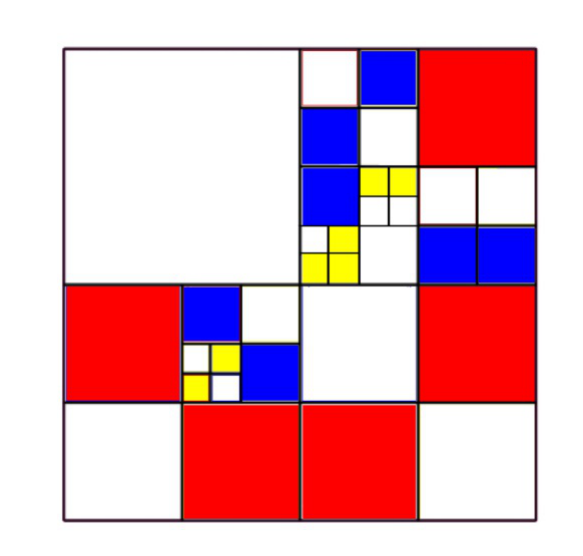
\includegraphics[width=0.35\textwidth]{figs/fig-2-1.png}
\caption{二进 Mondrian 图.}
\label{fig:2.1}
\end{figure}

\section{Vitali 覆盖}

设 $\mathcal{B}$ 是有限测度可测子集构成的族.

\begin{definition}\label{def:2.4}
族 $\mathcal{B}$ 具有 Vitali 覆盖性质 $\mathrm{V}_q$（$1 \leq q \leq \infty$）, 若存在有限常数 $C$, 使得对每一族 $\{R_i\}_{i \in I} \subset \mathcal{B}$, 都能找到子列 $\{\tilde{R}_k\}_{k \geq 1} \subset \{R_i\}_{i \in I}$, 满足下列条件:
\begin{align*}
  \mu\Big(\bigcup_{i\in I}R_{i}\Big)\leq C\,\mu\Big(\bigcup_{k}\tilde{R}_{k}\Big),
\end{align*}
\begin{align*}
  \Big\|\sum_{k}\chi_{\tilde{R}_{k}}\Big\|_{q}\leq C\,\mu\Big(\bigcup_{i\in I}R_{i}\Big)^{1/q}.
\end{align*}
这里我们使用了集合 $A$ 的示性函数的标准记号 $\chi_{A}$. 为简化表述, 且在不致混淆时, 我们将使用记号 $A(x) = \chi_{A}(x)$ 代替.
\end{definition}

\begin{theorem}\label{thm:2.5}
极大算子 $M$ 是弱型 $(p,p)$ 的, 当且仅当 $\mathcal{B}$ 满足覆盖性质 $\mathrm{V}_{q}$, 其中 $1/p+1/q=1$, $1<p<\infty$.
\end{theorem}

\begin{proof}
首先假设 $\mathcal{B}$ 具有性质 $\mathrm{V}_q$. 对 $\alpha > 0$, 令 $F_\alpha = \{x : M f(x) \geq \alpha\}$. 显然
\begin{align*}
  F_{\alpha}=\bigcup_{i\in I}R_{i},\qquad R_{i}\in\mathcal{B},
\end{align*}
且
\begin{align*}
  \frac{1}{\mu(R_{i})}\int_{R_{i}}\left|f(y)\right|\,\mathrm{d}\mu(y)>\alpha.
\end{align*}
按 $\mathrm{V}_q$ 定义选取 $\{\tilde{R}_k\}$. 则
\begin{align*}
  \mu(F_{\alpha})
  &=\mu\Big(\bigcup_{i} R_{i}\Big)\leq C\sum_{k}\mu(\tilde{R}_{k})
  \leq\frac{C}{\alpha}\sum_{k}\int_{\tilde{R}_{k}}|f(u)|\,\mathrm{d}\mu(u)\\
  &=\frac{C}{\alpha}\int\Big[\sum_{k}\tilde{R}_{k}(y)\Big]|f(y)|\,\mathrm{d}\mu(y)
  \leq\frac{C}{\alpha}\Big\|\sum_{k}\tilde{R}_{k}\Big\|_{q}\|f\|_{p}
  \leq\frac{C^{2}}{\alpha}\,\mu(F_{\alpha})^{1/q}\|f\|_{p},
\end{align*}
回忆 $1/p + 1/q = 1$, 由此得
\begin{align*}
  \mu(F_{\alpha})\leq C^{2p}\frac{\|f\|_{p}^{p}}{\alpha^{p}},
\end{align*}
即 $M$ 是弱型 $(p, p)$ 的.

反之, 设 $M$ 从 $L^p$ 到 Lorentz 空间 $L(p, \infty)$ 有界, 等价地, $M$ 是弱型 $(p, p)$ 的（\cite{b14} 含有本证明所需的 Lorentz 空间性质）. 给定陈述中的族 $\{R_i\}$, 假设存在子列 $\{\tilde{R}_k\}$, 满足 $\mu\bigl(\bigcup_i R_i\bigr) \leq C\,\mu\bigl(\bigcup_k \tilde{R}_k\bigr)$ 及下述\termcn{稀疏性}性质:
\begin{equation}\label{eq:2.3}
  \mu\Big\{\tilde{R}_{k}\cap\Big(\bigcup_{j<k}\tilde{R}_{j}\Big)\Big\}\leq\frac{1}{2}\,\mu(\tilde{R}_{k}),\quad k=1,2,\ldots.
\end{equation}
那么我们断言, 序列 $\{\tilde{R}_k\}$ 还满足 $\bigl\|\sum_k \tilde{R}_k\bigr\|_q \leq C\bigl(\bigcup_i R_i\bigr)^{1/q}$, 其中 $C < \infty$ 是某个普适常数. 为看出这一点, 令
\begin{align*}
  E_{k}=\tilde{R}_{k}\setminus\bigcup_{j<k}\tilde{R}_{j},
\end{align*}
定义线性算子
\begin{align*}
  T f(x)=\sum_{k}\left\{\frac{1}{\mu(\tilde{R}_{k})}\int_{\tilde{R}_{k}}f(y)\,\mathrm{d}\mu(y)\right\}\cdot\chi_{E_{k}}(x),
\end{align*}
并注意其伴随由下式给出:
\begin{align*}
  T^{*}f(x)=\sum_{k}\left\{\frac{1}{\mu(\tilde{R}_{k})}\int_{E_{k}}f(y)\,\mathrm{d}\mu(y)\right\}\cdot\chi_{\tilde{R}_{k}}(x).
\end{align*}
还要注意 $|Tf(x)| \leq Mf(x)$, 以及
\begin{align*}
  T^{*}\bigl(\chi_{\bigcup_{k}\tilde{R}_{k}}\bigr)(x)\geq\frac{1}{4}\sum_{k}\chi_{\tilde{R}_{k}}(x).
\end{align*}
由于（按假设）$M$ 从 $L^p$ 到 $L(p, \infty)$ 有界, 同样的结论对 $T$ 成立, 且界与 $\{\tilde{R}_k\}$ 无关. 由\newterm{duality}{对偶}{duality}, 算子 $T^*$ 必从 Lorentz 空间 $L(q,1)$ 到 $L^{q}$ 有界, 这蕴含
\begin{align*}
  \Big\|\sum_{k}\chi_{\tilde{R}_{k}}\Big\|_{q}\leq C\,\mu\Big(\bigcup_{k}\tilde{R}_{k}\Big)^{1/q},
\end{align*}
其中 $C$ 是依赖于 $M$ 的界、但不依赖于族 $\{R_{i}\}$ 的常数.

为结束证明, 必须说明如何选取具有稀疏性性质 \eqref{eq:2.3} 的序列 $\{R_k\}$. 首先, 不失一般性可设 $\{R_i\}$ 是序列 $\{R_1, R_2, \ldots\}$. 然后取 $\tilde{R}_1 = R_1$；假设已选定 $\tilde{R}_1, \ldots, \tilde{R}_k$, 取 $\tilde{R}_{k+1}$ 为序列 $\{R_i\}$ 中位于 $\tilde{R}_k$ 之后、具有性质
\begin{align*}
  \mu\Big(\tilde{R}_{k+1}\cap\Big(\bigcup_{j\leq k}\tilde{R}_{j}\Big)\Big)\leq\frac{1}{2}\,\mu(\tilde{R}_{k})
\end{align*}
的第一个元素, 并注意
\begin{align*}
  \bigcup_{j}R_{j}\subset\left\{x:M\bigl(\chi_{\bigcup_{k}\tilde{R}_{k}}\bigr)(x)\geq 1/2\right\}.
\end{align*}
\end{proof}

\begin{remark}\label{rem:2.6}
情形 $p = 1$, $q = \infty$ 不能加入定理的陈述, 因为两个蕴涵中只有一个成立. 即性质 $V_{\infty}$ 蕴含弱型 $(1, 1)$, 但反方向一般不成立. 然而, 极大函数的弱型 $(1, 1)$ 性质蕴含估计
\begin{align*}
  \int_{\bigcup_{k}R_{k}}\exp\Big(\sum_{k}\chi_{R_{k}}(x)\Big)\,\mathrm{d}\mu(x)\leq C\,\mu\Big(\bigcup_{k}R_{k}\Big)
\end{align*}
对每个满足稀疏性性质 \eqref{eq:2.3} 的序列 $\{R_{k}\}$ 成立.

一般地, 若 $M$ 从 $L(\log^{+}L)^{r}$ 到弱 $L^{1}$ 有界, 则满足稀疏性性质 \eqref{eq:2.3} 的序列必满足
\begin{equation}\label{eq:2.4}
  \int_{\bigcup_{k}R_{k}}\exp\Big(\sum_{k}\chi_{R_{k}}(x)\Big)^{1/(r+1)}\,\mathrm{d}\mu(x)\leq C\,\mu\Big(\bigcup_{k}R_{k}\Big).
\end{equation}
但这样的覆盖引理不足以保证极大函数算子从 $L(\log^{+}L)^{r}$ 到弱 $L^{1}$ 的有界性.

不等式 \eqref{eq:2.4} 的证明可以容易地由 Marcinkiewicz\newterm{interpolation}{插值}{interpolation}定理得到, 只需跟踪 $p \to 1$ 时 Hardy--Littlewood 极大函数在 $L^p(\R^n)$ 中估计常数的增长.
\end{remark}

\section{强极大函数}

现在考虑 $\R^n$ 上的 Lebesgue 测度以及各边平行于坐标轴的平行多面体（矩形）构成的族 $\mathcal{B}_n$. 再次得到相伴的极大函数 $M_n$, 对其所谓的强极大定理可以用两种等价形式陈述:

\begin{enumerate}
\item[(a)] 定量版本: $M_n$ 从 Orlicz 空间 $L(\log^+L)^{n-1}(\mathcal{Q})$ 到弱 $L^1(\mathcal{Q})$ 有界, 其中 $\mathcal{Q}$ 是 $\R^n$ 中的单位方体: 对 $\alpha > 0$,
\begin{align*}
  \mu\{M_{n}f(x)>\alpha\}\leq C_{n}\int_{\mathcal{Q}}\frac{|f(x)|}{\alpha}\Big\{1+\Big(\log^{+}\frac{|f(x)|}{\alpha}\Big)^{n-1}\Big\}\,\mathrm{d}\mu(x),
\end{align*}
其中 $C_{n}$ 是仅依赖于维数 $n$ 的常数；

\item[(b)] 定性版本: 基 $\mathcal{B}_n$ 微分属于空间 $L(\log^+ L)^{n-1}$ 的局部函数的积分, 即
\begin{align*}
  \lim_{\substack{x\in R\\ \mathrm{diam}(R)\to 0}}\frac{1}{\mu(R)}\int_{R}f(y)\,\mathrm{d}\mu(y)=f(x),\quad\text{a.e.}\ x\in\R^{n},
\end{align*}
对每个局部属于 $L(\log^{+}L)^{n-1}(\R^{n})$ 的函数 $f$ 成立.
\end{enumerate}

\newterm{strong-maximal-function}{强极大函数}{strong maximal function}在与多参数膨胀族交换的算子的研究中颇为要紧, 在这里参数的数目至关重要, 它改变结果的性质.

例如, 当 $n \geq 2$ 时, $M_n$ 不满足 Hardy--Littlewood 不等式. 例如, 当 $n = 2$ 时取
\begin{align*}
  f_{\varepsilon}(x_{1},x_{2})=\frac{1}{\varepsilon^{2}}\,\chi_{\{|x_{1}|<\varepsilon/2,\ |x_{2}|<\varepsilon/2\}},
\end{align*}
则对 $|x_1|, |x_2| > 2\varepsilon$, 有 $M_2f_\varepsilon(x_1, x_2) \sim 1/(|x_1|\,|x_2|)$.

设 $Q_{0} = [-1, 1] \times [-1, 1]$. 则
\begin{align*}
  \mu\{x\in Q_{0}:M_{2}f_{\varepsilon}>\lambda\}
  \geq\mu\{x\in Q_{0}:|x_{1}\cdot x_{2}|<1/\lambda\}
  \sim\frac{1}{\lambda}\left|\log\frac{1}{\lambda}\right|,\quad\text{若 } \lambda=1/\varepsilon,
\end{align*}
而我们想要的是与 Hardy--Littlewood 极大函数所满足者类似的不等式. 由此可知 $\|f_\varepsilon\| \geq c\log\frac{1}{\varepsilon}$, 而使其成立的最小 Orlicz 范数正是 $L(\log^+ L)$ 范数.

上面引述的结果 (a) 与 (b) 归功于 Jessen、Marcinkiewicz 与 Zygmund \cite{b57}. 其证明的主要思想是用复合 $M_{x_1} \cdot M_{x_2} \cdots M_{x_n}$ 来控制算子 $M_n$, 其中 $M_{x_j}$ 表示沿第 $j$ 个坐标轴方向的一维 Hardy--Littlewood 极大算子. 该论证的优雅与简洁是显然的. 然而, 似乎宜于有一个基于恰当覆盖引理的几何证明. 主要原因是, 对别的测度我们缺乏乘积结构, 而获得与强极大函数类似算子的结果的唯一途径, 是通过对\newterm{rectangle}{矩形}{rectangle}几何的深刻理解.

图~\ref{fig:2.2} 表明 Vitali 覆盖引理对 $\R^n$（$n \geq 2$）中的平行多面体不成立. 注意 $\mu(R_1) = \mu(R_2) = \cdots = \mu(R_k) = 1$. 矩形序列 $\{R_k\}$ 满足性质 \eqref{eq:2.3}, 但没有任何办法选出满足 Vitali 覆盖要求的子族.

\begin{figure}[htbp]
\centering
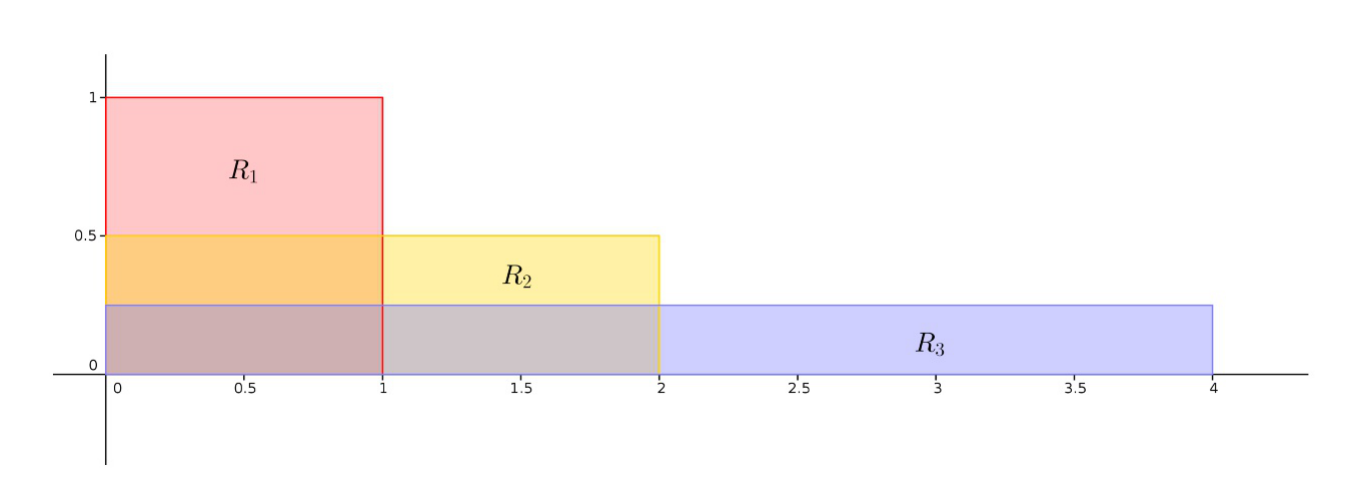
\includegraphics[width=0.72\textwidth]{figs/fig-2-2.png}
\caption{Vitali 覆盖引理对平行多面体不成立.}
\label{fig:2.2}
\end{figure}

\begin{theorem}\label{thm:2.7}
设 $\{R_k\}$ 是 $\R^n$ 中一列各边平行于坐标轴的平行多面体, 其并集有界. 则存在子列 $\{\tilde{R}_j\} \subset \{R_k\}$, 使得
\begin{enumerate}
\item[(1)] $\mu\Big(\bigcup_{k}R_{k}\Big)\leq C_{n}\,\mu\Big(\bigcup_{j}\tilde{R}_{j}\Big)$；
\item[(2)] $\Big\|\exp\Big(\sum_{j}\chi_{\tilde{R}_j}\Big)^{1/(n-1)}-1\Big\|_1 \leq C_n\,\mu\Big(\bigcup_j \tilde{R}_j\Big)$, 其中 $C_n < \infty$ 是普适常数.
\end{enumerate}
\end{theorem}

在证明这一定理之前, 让我们说明它蕴含上述 Jessen、Marcinkiewicz 与 Zygmund 的结果. 设 $\alpha > 0$. 对每个点 $x \in \{M_n f(x) > \alpha\}$, 存在含 $x$ 的矩形 $R_x$, 满足
\begin{align*}
  \frac{1}{\left|R_{x}\right|}\int_{R_{x}}\left|f\right|>\alpha.
\end{align*}
不失一般性, 假设 $\bigcup_x R_x = \bigcup_k R_k$, 其中 $R_k$ 是某些 $R_x$. 应用覆盖引理得到满足定理 2.7 中性质 (1) 与 (2) 的 $\tilde{R}_k$. 于是由 (1), 只须证明
\begin{align*}
  \mu\Big(\bigcup_{k}\tilde{R}_{k}\Big)\leq C_{n}\int_{\R^{n}}\frac{|f(x)|}{\alpha}\log^{n-1}\left(1+\frac{|f(x)|}{\alpha}\right)\mathrm{d}x.
\end{align*}
由于 $\mu(R_k) \leq \frac{1}{\alpha} \int_{R_k} |f|$, 求和得
\begin{align*}
  \mu\Big(\bigcup_{k}\tilde{R}_{k}\Big)\leq\frac{1}{\alpha}\int_{Q_{0}}|f|\sum_{k}\chi_{\tilde{R}_{k}}.
\end{align*}
适当应用 Young 不等式 $ab \leq e^a - b + b\log b$（$a, b > 0$）, 即得结果.

\begin{proof}[定理~\ref{thm:2.7} 的证明]
我们对 $n$ 作归纳. 假设 $n-1$ 的情形, 并把 $R_1, R_2, \ldots$ 排列成 $x_n$ 方向边长递减的顺序. 对矩形 $R$, 用 $R_d$ 表示与 $R$ 同心、对 $i < n$ 各 $x_i$ 方向边长相同、但 $x_n$ 方向边长乘以 $5$ 的矩形. 下面描述从 $R_k$ 中选取 $\tilde{R}_k$ 的程序. 令 $\tilde{R}_1 = R_1$. 假设 $\tilde{R}_1, \tilde{R}_2, \ldots, \tilde{R}_k$ 已经选定. 我们继续沿列表前行, 每次考虑矩形 $R$ 时, 询问是否
\begin{align*}
  \mu\Big(R\cap\Big(\bigcup_{j}(\tilde{R}_{j})_{d}\Big)\Big)<\frac{1}{2}\,\mu(R),
\end{align*}
其中上面的并取遍满足 $\tilde{R}_j \cap R \neq \emptyset$ 的一切 $j \leq k$. 若答案是否定的, 就移到列表的下一个矩形. 若答案是肯定的, 就把这个矩形 $R$ 定为 $\tilde{R}_{k+1}$, 并重新开始这一过程.

现在如下证明 (1). 若 $R$ 是未被选中的矩形, 则
\begin{align*}
  \mu\Biggl(R\cap\Big[\bigcup_{\substack{\tilde{R}_{j}\cap R\neq\emptyset\\ \tilde{R}_{j}\ \text{在}\ R\ \text{之前}}}(\tilde{R}_{j})_{d}\Big]\Biggr)\geq\frac{1}{2}\,\mu(R).
\end{align*}
用垂直于 $x_n$ 轴的超平面把所有矩形切片. 若切片用 $S$ 代替 $R$ 表示, 则
\begin{align*}
  \mu\Big(S\cap\Big(\bigcup_{j}(\tilde{S}_{j})_{d}\Big)\Big)\geq\frac{1}{2}\,\mu(S),
\end{align*}
从而在 $\bigcup_{j}R_{j}$ 上有
\begin{align*}
  M_{n-1}\bigl(\chi_{\bigcup_{j}(\tilde{R}_{j})_{d}}\bigr)>1/2,
\end{align*}
其中 $M_{n-1}$ 作用于 $x_1, x_2, \ldots, x_{n-1}$ 坐标.

由 $M_{n-1}$ 在（比如）$L^2$ 上的有界性（归纳假设）, 得
\begin{align*}
  \mu\Big(\bigcup_{j}R_{j}\Big)\leq C\,\mu\Big(\bigcup_{k}(\tilde{R}_{k})_{d}\Big)
  \leq C^{\prime}\sum_{k}\mu(\tilde{R}_{k})
  \leq C^{\prime}\,\mu\Big(\bigcup_{k}\tilde{R}_{k}\Big).
\end{align*}

为得到 (2), 注意诸 $\tilde{R}_{j}$ 满足
\begin{align*}
  \mu\Biggl(\tilde{R}_{k}\cap\Big[\bigcup_{\substack{\tilde{R}_{j}\cap\tilde{R}_{k}\neq\emptyset\\ j<k}}(\tilde{R}_{j})_{d}\Big]\Biggr)<\frac{1}{2}\,\mu(\tilde{R}_{k}).
\end{align*}
再用垂直于 $x_{n}$ 轴的超平面切片, 得到
\begin{align*}
  \mu\Big(\tilde{S}_{k}\cap\Big(\bigcup_{j<k}\tilde{S}_{j}\Big)\Big)<\frac{1}{2}\,\mu(\tilde{S}_{k}),
\end{align*}
故若令
\begin{align*}
  \widetilde{E}_{k}=\widetilde{S}_{k}\setminus\bigcup_{j<k}\widetilde{S}_{j},
\end{align*}
则有 $\mu(\widetilde{E}_k) > \frac{1}{2}\,\mu(\widetilde{S}_k)$；且若 $\phi \in L(\log L)^{n-1}(S_0)$, 我们将证明
\begin{equation}\label{eq:2.5}
  \int_{S_{0}}\sum_{k}\chi_{\tilde{S}_{k}}\,\phi\leq C\left\|\phi\right\|_{L(\log L)^{n-1}},
\end{equation}
由此得到
\begin{align*}
  \int_{S_{0}}\exp\left[c\Big(\sum_{k}\chi_{\tilde{S}_{k}}\Big)^{1/(n-1)}\right]\mathrm{d}x_{1}\cdots\mathrm{d}x_{n-1}\leq C.
\end{align*}
把这个估计对 $x_{n}$ 积分即可结束.

为得到 \eqref{eq:2.5}, 我们写
\begin{align*}
  \int_{S_{0}}\sum_{k}\chi_{\tilde{S}_{k}}\,\phi\;\mathrm{d}x_{1}\cdots\mathrm{d}x_{n-1}
  &\leq\sum_{k}\int_{\tilde{S}_{k}}\phi
  \leq C\sum_{k}|\widetilde{E}_{k}|\,\frac{1}{|\tilde{S}_{k}|}\int_{\tilde{S}_{k}}\phi\\
  &\leq C\int_{S_{0}}M_{n-1}(\phi)\;\mathrm{d}x_{1}\mathrm{d}x_{2}\cdots\mathrm{d}x_{n-1}
  \leq C^{\prime}\|\phi\|_{L(\log L)^{n-1}}.
\end{align*}

在上述论证中, 切片是最重要的思想. 若不切片而直接尝试证明, 我们得到的将不是 $\exp(\cdot)^{1/(n-1)}$ 范数上的估计, 而是 $\exp(\cdot)^{1/n}$ 范数上的估计. 而且, 切片正是我们用以用较低参数算子 $M_{n-1}$ 控制 $M_n$ 的机制, 这使我们能够进行归纳.
\end{proof}

\begin{figure}[htbp]
\centering
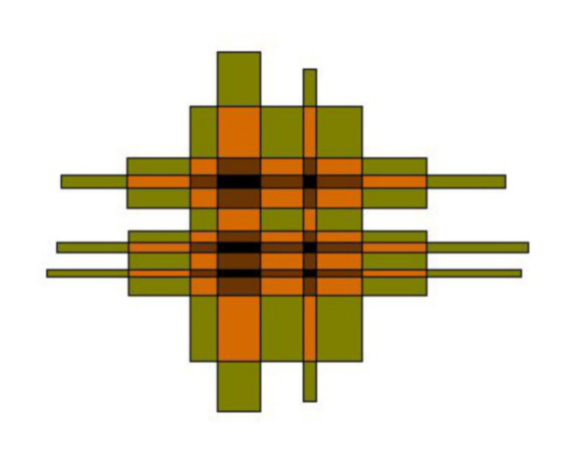
\includegraphics[width=0.42\textwidth]{figs/fig-2-3.png}
\caption{指数重叠.}
\label{fig:2.3}
\end{figure}

\section{A. Zygmund 的一个问题}

设 $\phi$ 是 $\R^2$ 中一个对每个变量分别单调的正函数. 考虑族 $\mathcal{B}_\phi = \mathcal{B}_2 \times \phi$, 即各边垂直于坐标轴、尺寸为 $s \times t \times \phi(s, t)$（$s$、$t$ 为正实数）的平行多面体. 注意, 强极大定理断言: 由于 $\mathcal{B}_\phi \subset \mathcal{B}_3$, 它微分局部属于 $L(\log^{+}L)^2(\R^3)$ 的函数的积分.

然而, 由于族 $\mathcal{B}_{\phi}$ 的平行多面体的竖直方向受限于某个单调函数的图象, 我们可以指望得到一些额外的正则性, 但要记住, 我们不可能得到比 $\mathcal{B}_2$ 更好的微分性质. 事实上, 我们将证明最优的可能改进已经达到. 让我们用两种等价形式陈述结果.

\begin{theorem}\label{thm:2.8}
\begin{enumerate}
\item[(1)] 平行多面体族 $\mathcal{B}_\phi$ 微分局部属于 $L(\log^+L)(\R^3)$ 的函数的积分, 即
\begin{align*}
  \lim_{R\to x}\frac{1}{\mu(R)}\int_{R} f(y)\,\mathrm{d}\mu(y)=f(x),\quad\text{a.e.}\ x,
\end{align*}
只要 $f \in L(\log^{+}L)(\R^{3})$, 其中 $\mu$ 表示 $\R^{3}$ 中的 Lebesgue 测度.

\item[(2)] 相伴的极大函数
\begin{align*}
  M_{\phi}f(x)=\sup_{R\ni x}\frac{1}{\mu(R)}\int_{R}\left|f(y)\right|\,\mathrm{d}\mu(y)
\end{align*}
满足不等式
\begin{align*}
  \mu\{x:M_{\phi}f(x)>\lambda\}\leq C\int\frac{|f(y)|}{\lambda}\left(1+\log^{+}\frac{|f(y)|}{\lambda}\right)\mathrm{d}\mu(y),
\end{align*}
其中 $C < \infty$ 是某个普适常数.
\end{enumerate}
\end{theorem}

为证明这一结果, 我们将再一次为族 $\mathcal{B}_{\phi}$ 发展一个合适的覆盖引理. 先引入一个定义.

\begin{definition}\label{def:2.9}
称 $\R^3$ 中平行多面体的族 $\mathcal{B}$ 是单调的, 若给定尺寸分别为 $s_1 \times t_1 \times u_1$ 与 $s_2 \times t_2 \times u_2$ 的任意两个平行多面体 $R_1$ 与 $R_2$, 下列蕴涵成立: 若 $s_1 < s_2$ 且 $t_1 < t_2$, 则 $u_1 \leq u_2$.
\end{definition}

为简化直觉与计算, 我们将局限于单调族 $\mathcal{B}$ 的平行多面体为\newterm{dyadic}{二进的}{dyadic}的情形. 下面的覆盖引理将蕴含定理 2.8.

\begin{lemma}\label{lem:2.10}
设 $\mathcal{B}$ 是 $\R^3$ 中单调的二进平行多面体族. 对满足 $\mu\bigl(\bigcup_{i\in I} R_i\bigr) < \infty$ 的每一族 $\{R_i\}_{i\in I} \subset \mathcal{B}$, 都能找到有限子列 $\{\tilde{R}_j\}_{j=1}^M \subset \{R_i\}_{i\in I}$, 同时满足
\begin{align*}
  \mu\Big(\bigcup_{i\in I}R_{i}\Big)\leq C\,\mu\Big(\bigcup_{j=1}^{M}\tilde{R}_{j}\Big),
\end{align*}
\begin{align*}
  \int_{\bigcup_{j=1}^{M}\tilde{R}_{j}}\exp\Big(\sum_{j=1}^{M}\chi_{\tilde{R}_{j}}(x)\Big)\,\mathrm{d}\mu(x)
  \leq C\,\mu\Big(\bigcup_{j=1}^{M}\tilde{R}_{j}\Big),
\end{align*}
其中 $C < \infty$ 是普适常数.
\end{lemma}

\begin{proof}
首先注意, 由于 $\mu\bigl(\bigcup_i R_i\bigr) < \infty$, 不失一般性可设 $\{R_i\}_{i \in I}$ 是有限序列 $\{R_i\}_{i=1}^N$, 使得
\begin{align*}
  \mu\Big(R_{i}\cap\Big(\bigcup_{j\neq i}R_{j}\Big)\Big)\leq\frac{1}{2}\,\mu(R_{i}),\quad i=1,\ldots,N.
\end{align*}
此外, 把序列重新排列, 使平行多面体的 $x_3$ 方向尺寸 $d_3(R_i)$ 递减, 即
\begin{align*}
  d_{3}(R_{k})\geq d_{3}(R_{k+1}),\quad k=1,2,\ldots .
\end{align*}
我们以选取 $\tilde{R}_1 = R_1$ 开始选择过程. 然后取 $\tilde{R}_k$ 为序列中满足
\begin{equation}\label{eq:2.6}
  \int_{\tilde{R}_{k}}\exp\Big(\sum_{j=1}^{k-1}\tilde{R}_{j}(x)\Big)\,\mathrm{d}\mu(x)
  \leq(1+e^{-1})\,\mu(\tilde{R}_{k})
\end{equation}
的下一个元素. 注意, $e^{-1}$ 可以换成某个别的适当常数. 下面将证明序列 $\{\tilde{R}_k\}_{k=1}^M$ 满足性质 (2):
\begin{align*}
  \int_{\bigcup_{j=1}^{M}\widetilde{R}_{j}}&\exp\left(\sum_{j=1}^{M}\chi_{\widetilde{R}_{j}}(x)\right)\mathrm{d}\mu(x)\\
  &=\int_{\bigcup_{j=1}^{M-1}\widetilde{R}_{j}\setminus\widetilde{R}_{M}}\exp\left(\sum_{j=1}^{M-1}\chi_{\widetilde{R}_{j}}(x)\right)\mathrm{d}\mu(x)
   +\int_{\widetilde{R}_{M}}\exp\left(\sum_{j=1}^{M}\chi_{\widetilde{R}_{j}}(x)\right)\mathrm{d}\mu(x)\\
  &=\int_{\bigcup_{j=1}^{M-1}\widetilde{R}_{j}\setminus\widetilde{R}_{M}}\exp\left(\sum_{j=1}^{M-1}\chi_{\widetilde{R}_{j}}(x)\right)\mathrm{d}\mu(x)
   +e\int_{\widetilde{R}_{M}}\exp\left(\sum_{j=1}^{M-1}\chi_{\widetilde{R}_{j}}(x)\right)\mathrm{d}\mu(x).
\end{align*}
但根据我们的选取 \eqref{eq:2.6}, 第二个积分项可以被控制, 于是得
\begin{align*}
  \int_{\bigcup_{j=1}^{M}\tilde{R}_{j}}\exp\Big(&\sum_{j=1}^{M}\chi_{\tilde{R}_{j}}(x)\Big)\mathrm{d}\mu(x)\\
  &\leq\int_{\bigcup_{j=1}^{M-1}\tilde{R}_{j}}\exp\Big(\sum_{j=1}^{M-1}\chi_{\tilde{R}_{j}}(x)\Big)\mathrm{d}\mu(x)+(1+e)\,\mu(\tilde{R}_{M}).
\end{align*}
迭代这一过程, 得到如下控制:
\begin{align*}
  \int_{\bigcup_{j=1}^{M}\tilde{R}_{j}}\exp\Big(\sum_{j=1}^{M}\chi_{\tilde{R}_{j}}(x)\Big)\mathrm{d}\mu(x)
  \leq(1+e)\sum_{k=1}^{M}\mu(\tilde{R}_{k})
  \leq 2(1+e)\,\mu\Big(\bigcup_{k=1}^{M}\tilde{R}_{k}\Big).
\end{align*}

我们的目标现在是证明我们没有丢弃``太多''平行多面体, 即
\begin{align*}
  \mu\Big(\bigcup_{i=1}^{N} R_{i}\Big)\leq C\,\mu\Big(\bigcup_{j=1}^{M}\tilde{R}_{j}\Big).
\end{align*}
设 $R$ 是被丢弃的平行多面体. 则由于族 $\{\tilde{R}_j\}_{j=1}^M$ 已经按竖直尺寸 $d_3(\tilde{R}_j)$ 递减排列, 必有
\begin{align*}
  1+e^{-1}<\frac{1}{\mu(R)}\int_{R}\exp\Big(\sum_{d_{3}(\tilde{R}_{j})\geq d_{3}(R)}\chi_{\tilde{R}_{j}}(x)\Big)\mathrm{d}\mu(x).
\end{align*}
注意, 由于族 $\mathcal{B}_\phi$ 是单调的, 若 $d_3(\tilde{R}_j) \geq d_3(R)$, 则必有
\begin{align*}
  d_{1}(\tilde{R}_{j})\geq d_{1}(R)\quad\text{或}\quad d_{2}(\tilde{R}_{j})\geq d_{2}(R).
\end{align*}
于是可以把上面的不等式改写成
\begin{equation}\label{eq:2.7}
  \begin{aligned}
  1+e^{-1}&<\frac{1}{\mu(R)}\int_{R}\exp\left(\sum_{\substack{d_{3}(\tilde{R}_{j})\geq d_{3}(R)\\ d_{1}(\tilde{R}_{j})\geq d_{1}(R)}}\chi_{\tilde{R}_{j}}(x)\right)
   \cdot\exp\left(\sum_{\substack{d_{3}(\tilde{R}_{j})\geq d_{3}(R)\\ d_{2}(\tilde{R}_{j})\geq d_{2}(R)}}\chi_{\tilde{R}_{j}}(x)\right)\mathrm{d}\mu(x)\\
  &=\frac{1}{\mu(R)}\int_{R}\exp\left(\sum_{i=1}^{k}\chi_{\tilde{R}_{\nu_{i}}}(x)\right)
   \cdot\exp\left(\sum_{j=1}^{l}\chi_{\tilde{R}_{\mu_{j}}}(x)\right)\mathrm{d}\mu(x),
  \end{aligned}
\end{equation}
其中 $\tilde{R}_{\nu_1}, \ldots, \tilde{R}_{\nu_k}$ 是第一个和中的平行多面体, $\tilde{R}_{\mu_1}, \ldots, \tilde{R}_{\mu_l}$ 是第二个和中的那些.

固定平行多面体 $R$, 不失一般性, 可简化记号, 改换指标使得对 $i = 1, \ldots, k$ 有 $\tilde{R}_{\nu_i} = \tilde{R}_i$, 对 $j = 1, \ldots, l$ 有 $\tilde{R}_{\mu_j} = \tilde{R}_{k+j}$. 现在把积分号内的指数展开:
\begin{align*}
  \exp\Big(\sum_{i=1}^{k}\chi_{\tilde{R}_{\nu_{i}}}(x)\Big)
  &=\sum_{n=0}^{\infty}\frac{1}{n!}\Big(\sum_{i=1}^{k}\chi_{\tilde{R}_{\nu_{i}}}(x)\Big)^{n}
  =\sum_{n=0}^{\infty}\frac{1}{n!}\sum_{i_{1},\ldots,i_{n}=1}^{k}
   \chi_{\tilde{R}_{i_{1}}}(x)\cdots\chi_{\tilde{R}_{i_{n}}}(x),\\
  \exp\Big(\sum_{j=1}^{l}\chi_{\tilde{R}_{\mu_{j}}}(x)\Big)
  &=\sum_{m=0}^{\infty}\frac{1}{m!}\Big(\sum_{j=1}^{l}\chi_{\tilde{R}_{\mu_{j}}}(x)\Big)^{m}
  =\sum_{m=0}^{\infty}\frac{1}{m!}\sum_{j_{1},\ldots,j_{m}=k+1}^{k+l}
   \chi_{\tilde{R}_{j_{1}}}(x)\cdots\chi_{\tilde{R}_{j_{m}}}(x).
\end{align*}
最后这些和式项正是 $n$ 个因子 $\chi_{\tilde{R}_{\nu_{i}}}$（或分别地, $m$ 个因子 $\chi_{\tilde{R}_{\mu_{i}}}$）乘积的所有可能组合. 因此, 把这个表达式用于 \eqref{eq:2.7}, 得到
\begin{align*}
  \sum_{n,m=0}^{\infty}&\frac{1}{n!\,m!}\sum_{i_{1},\ldots,i_{n}=1}^{k}\sum_{j_{1},\ldots,j_{m}=k+1}^{k+l}
  \frac{1}{\mu(R)}\int_{R}\chi_{\tilde{R}_{i_{1}}}(x)\cdots\chi_{\tilde{R}_{j_{m}}}(x)\,\mathrm{d}\mu(x)\\
  &=\sum_{n,m=0}^{\infty}\frac{1}{n!\,m!}\sum_{i_{1},\ldots,i_{n}=1}^{k}\sum_{j_{1},\ldots,j_{m}=k+1}^{k+l}
  \frac{\mu\{\tilde{R}_{i_{1}}\cap\cdots\cap\tilde{R}_{i_{n}}\cap\tilde{R}_{j_{1}}\cap\cdots\cap\tilde{R}_{j_{m}}\cap R\}}{\mu(R)}.
\end{align*}

现在很清楚, 为证明性质 (1), 关键在于控制平行多面体 $\tilde{R}_{i_1}, \ldots, \tilde{R}_{j_m}$ 与 $R$ 的重叠. 注意, 若相交不空, 则交集必呈图~\ref{fig:2.4} 所示的形状. 即, 对应于 $\varepsilon$ 的块是 $\tilde{R}_{i_1}, \ldots, \tilde{R}_{i_n}$ 的交, 对应于 $\delta$ 的块是 $\tilde{R}_{j_1}, \ldots, \tilde{R}_{j_m}$ 的交. 注意这里我们使用了所处理的是二进平行多面体这一事实: 若交集不空, 则切口必须是``干净的'', 即某一边尺寸较长的平行多面体把其余者沿该边方向完全切开.

\begin{figure}[htbp]
\centering
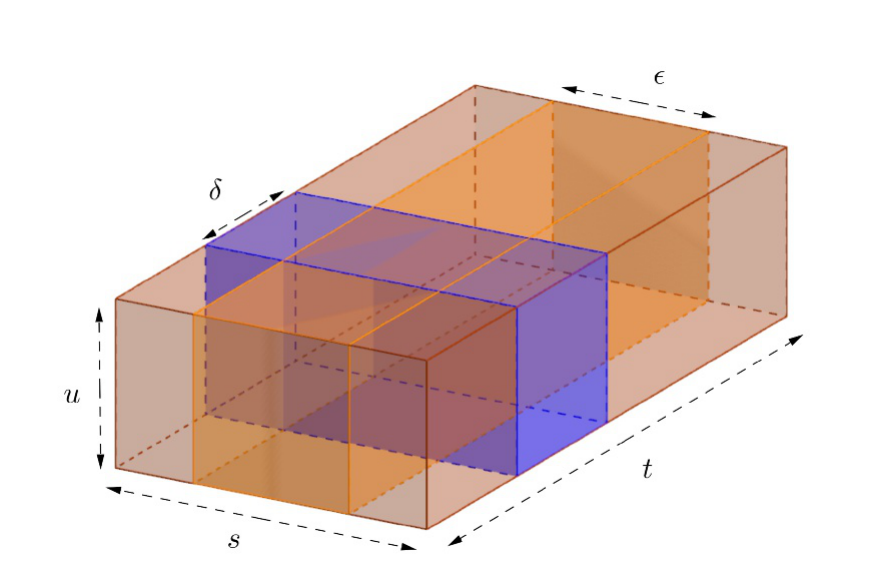
\includegraphics[width=0.45\textwidth]{figs/fig-2-4.png}
\caption{控制交集.}
\label{fig:2.4}
\end{figure}

于是交集 $\tilde{R}_{i_1} \cap \cdots \cap R_{i_n} \cap \tilde{R}_{j_1} \cap \cdots \cap \tilde{R}_{j_m}$ 将是尺寸为 $\varepsilon \times \delta \times u$ 的平行多面体. 由此得
\begin{align*}
  \frac{\mu\{\tilde{R}_{i_{1}}\cap\cdots\cap\tilde{R}_{i_{n}}\cap\tilde{R}_{j_{1}}\cap\cdots\cap\tilde{R}_{j_{m}}\cap R\}}{\mu(R)}
  =\frac{\varepsilon\times\delta}{s\times t},
\end{align*}
并且有
\begin{equation}\label{eq:2.8}
  1+e^{-1}<\sum_{n,m=0}^{\infty}\frac{1}{n!\,m!}\sum_{i_{1},\ldots,i_{n}=1}^{k}\sum_{j_{1},\ldots,j_{m}=k+1}^{k+l}\frac{\varepsilon\times\delta}{s\times t}.
\end{equation}

接下来更仔细地考察所有这些平行多面体的交集. 这次固定交集内的一点 $P = (x_0, y_0, z_0)$, 考虑与 $R$ 相交的水平平面与竖直平面（见图~\ref{fig:2.5}）以及线段
\begin{align*}
  I_{P}^{1}=\{\left(x,y_{0},z_{0}\right)\in R\},\qquad
  I_{P}^{2}=\{\left(x_{0},y,z_{0}\right)\in R\}.
\end{align*}

\begin{figure}[htbp]
\centering
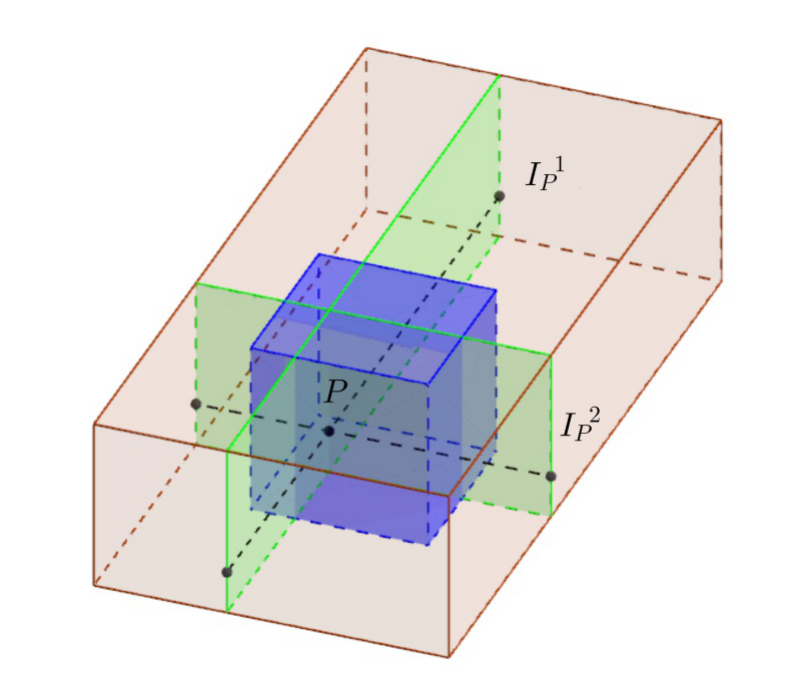
\includegraphics[width=0.4\textwidth]{figs/fig-2-5.png}
\caption{线段 $I_{P}^{1}$ 与 $I_{P}^{2}$.}
\label{fig:2.5}
\end{figure}

由单调性, 得
\begin{align*}
  \frac{|\tilde{R}_{i_{1}}\cap\cdots\cap\tilde{R}_{i_{n}}\cap I_{P}^{1}|}{|I_{P}^{1}|}=\frac{\varepsilon}{s},\qquad
  \frac{|\tilde{R}_{j_{1}}\cap\cdots\cap\tilde{R}_{j_{m}}\cap I_{P}^{2}|}{|I_{P}^{2}|}=\frac{\delta}{t}.
\end{align*}
这里 $|\cdot|$ 指一维 Lebesgue 测度. 把这两个量之积代入 \eqref{eq:2.8}, 得到方向 Hardy--Littlewood 极大函数的一个下界:
\begin{align*}
  1+e^{-1}
  &<\sum_{n,m=0}^{\infty}\frac{1}{n!\,m!}\sum_{i_{1},\ldots,i_{n}=1}^{k}\sum_{j_{1},\ldots,j_{m}=k+1}^{k+l}
   \frac{|\tilde{R}_{i_{1}}\cap\cdots\cap\tilde{R}_{i_{n}}\cap I_{P}^{1}|}{|I_{P}^{1}|}
   \cdot\frac{|\tilde{R}_{j_{1}}\cap\cdots\cap\tilde{R}_{j_{m}}\cap I_{P}^{2}|}{|I_{P}^{2}|},
\end{align*}
因此
\begin{align*}
  1+e^{-1}
  &<\Big\{\frac{1}{|I_{P}^{1}|}\int_{I_{P}^{1}}\exp\Big(\sum_{i=1}^{k}\chi_{\tilde{R}_{i}}(x)\Big)\mathrm{d}x\Big\}
   \cdot\Big\{\frac{1}{|I_{P}^{2}|}\int_{I_{P}^{2}}\exp\Big(\sum_{j=k+1}^{k+l}\chi_{\tilde{R}_{j}}(x)\Big)\mathrm{d}x\Big\}\\
  &<M_{1}\Big(\exp\Big(\sum_{i=1}^{k}\chi_{\tilde{R}_{i}}(x)\Big)\Big)(P)
   \cdot M_{2}\Big(\exp\Big(\sum_{j=k+1}^{k+l}\chi_{\tilde{R}_{j}}(x)\Big)\Big)(P),
\end{align*}
其中 $M_1$ 与 $M_2$ 分别表示沿 $x_1$ 与 $x_2$ 方向的一维 Hardy--Littlewood 极大函数到 $\R^3$ 上的扩张. 我们已证明, 对任何被丢弃的平行多面体, 有下面的包含关系:
\begin{align*}
  R&\subset\Big\{x:M_{1}\Big(\exp\Big(\sum_{i=1}^{M}\chi_{\tilde{R}_{i}}\Big)\Big)
   \cdot M_{2}\Big(\exp\Big(\sum_{j=1}^{M}\chi_{\tilde{R}_{j}}(x)\Big)\Big)>1+e^{-1}\Big\}\\
  &\subset\Big\{x:M_{1}\Big(\exp\Big(\sum_{i=1}^{M}\chi_{\tilde{R}_{i}}\Big)\Big)>\sqrt{1+e^{-1}}\Big\}
   \cup\Big\{x:M_{2}\Big(\exp\Big(\sum_{j=1}^{M}\chi_{\tilde{R}_{j}}(x)\Big)\Big)>\sqrt{1+e^{-1}}\Big\}.
\end{align*}
最后,
\begin{align*}
  \mu\Big(\bigcup_{i\in I}R_{i}\Big)
  &\leq\frac{2}{\sqrt{1+e^{-1}}}\int_{\bigcup_{j=1}^{M}\tilde{R}_{j}}\exp\Big(\sum_{j=1}^{M}\chi_{\tilde{R}_{j}}(x)\Big)\mathrm{d}\mu(x)\\
  &\leq 4\sqrt{1+e^{-1}}\;\mu\Big(\bigcup_{j=1}^{M}\tilde{R}_{j}\Big).
\end{align*}
\end{proof}

\begin{proof}[定理~\ref{thm:2.8} 的证明]
众所周知 (1) 与 (2) 是等价的, 其中蕴涵 (2) $\Rightarrow$ (1) 是较容易的一个. 证明的策略如下: 首先观察到, 若族 $\mathcal{B}$ 满足覆盖引理的假设, $M$ 表示与 $\mathcal{B}$ 相伴的极大函数, 则 $M$ 满足 (2). 接着, 我们找到具有性质 $M_{\phi}f \leq CMf$（$C$ 为普适常数）的这样的族 $\mathcal{B}$.

设 $\mathcal{B}$ 满足覆盖引理的假设, 定义
\begin{align*}
  M f(x)=\sup_{x\in R^{*},\;R\in\mathcal{B}}\frac{1}{\mu(R)}\int_{R}|f(y)|\,\mathrm{d}\mu(y),
\end{align*}
其中 $R^{*}$ 是把 $R$ 关于其中心以因子 $3$ 膨胀的结果.

\begin{claim*}
存在常数 $C < \infty$, 使得
\begin{align*}
  \mu(\{M f(x)>\lambda\})\leq C\int_{\R^{3}}\frac{|f(x)|}{\lambda}\left\{1+\log^{+}\frac{|f(x)|}{\lambda}\right\}\mathrm{d}\mu(x).
\end{align*}
\end{claim*}

\begin{proof}[断言的证明]
集合 $\{Mf(x) > \lambda\}$ 是满足
\begin{align*}
  \frac{1}{\mu(R_{\alpha})}\int_{R_{\alpha}}\left|f(y)\right|\,\mathrm{d}\mu(y)\geq\lambda
\end{align*}
的平行多面体 $\{R_\alpha\}$ 之并. 可以应用覆盖引理证明具有给定性质的子族 $\{R_{j}\}$ 的存在性. 我们有
\begin{align*}
  \mu\Big(\bigcup_{j}R_{j}^{*}\Big)
  \leq 27\sum_{j}\mu\Big(\bigcup_{j}R_{j}\Big)
  \leq 27\int_{\bigcup_{j}R_{j}}\frac{|f(x)|}{\lambda}\sum_{j}\chi_{R_{j}}(x)\,\mathrm{d}\mu(x).
\end{align*}
其次注意, 若 $u$ 与 $v$ 是正实数, 则 $u\cdot v \leq u\log u + e^{v-1}$. 此外, 对每个 $\varepsilon > 0$, 存在常数 $C_\varepsilon < \infty$, 使得 $u\cdot v \leq C_\varepsilon\,u(1 + \log^+ u) + e^{\varepsilon v - 1}$. 特别地,
\begin{align*}
  \mu\Big(\bigcup_{j} R_{j}^{*}\Big)
  \leq&\,C_{\varepsilon}\int_{\bigcup_{j} R_{j}}\frac{|f(x)|}{\lambda}\left\{1+\log^{+}\frac{|f(x)|}{\lambda}\right\}\mathrm{d}\mu(x)\\
  &+e^{-1}\int_{\bigcup_{j} R_{j}}\exp\Big(\varepsilon\sum_{j}\chi_{R_{j}}(x)\Big)\mathrm{d}\mu(x).
\end{align*}
但
\begin{align*}
  \int_{\bigcup_{j}R_{j}}&\exp\Big(\varepsilon\sum_{j}\chi_{R_{j}}(x)\Big)\mathrm{d}\mu(x)\\
  &\leq\Big[\mu\Big(\bigcup_{j}R_{j}\Big)\Big]^{1-\varepsilon}
   \Big(\int_{\bigcup_{j}R_{j}}\exp\Big(\sum_{j}\chi_{R_{j}}(x)\Big)\mathrm{d}\mu(x)\Big)^{\varepsilon}
  \leq C^{\varepsilon}\,\mu\Big(\bigcup_{j}R_{j}\Big),
\end{align*}
其中 $C$ 是覆盖引理中出现的常数. 为结束证明, 只需选取 $\varepsilon > 0$ 使 $C^{\varepsilon}e^{-1} \leq 1/2$.
\end{proof}

最后, 必须说明如何从 $\mathcal{B}_\phi$ 得到族 $\mathcal{B}$. 首先, 把 $s$ 与 $t$ 的值化入集合 $\{2^n\}_{n\in\Z}$. 然后定义 $\tilde{\phi}(2^k, 2^l) = 2^m$, 若 $2^{m-1} < \phi(2^k, 2^l) \leq 2^m$. 显然, 用这种方式得到的平行多面体族 $\mathcal{B}$ 中, $\mathcal{B}_\phi$ 的每个元素 $R$ 都包含于 $\tilde{\mathcal{B}}$ 的某个元素 $\tilde{R}$, 且 $\mu(\tilde{R}) \leq 8\mu(R)$. 接着, 在水平平面 $z = 0$ 上考虑二进矩形族, 对每个这样的矩形, 附上一个以该矩形为水平底面、竖直尺寸由 $\tilde{\phi}$ 给出的平行多面体. 然后把每个这样的平行多面体沿竖直方向平移其竖直长度的整数倍. 所得的族就是 $\mathcal{B}$. 显然 $M_\phi f(x) \leq 8M f(x)$.
\end{proof}

定理 2.8 对 Siegel 广义上半空间中的 Poisson 积分收敛有重要应用. 这里 $\R^n$ 被实现为 $M_n$, 即 $m \times m$ 实对称矩阵空间, $n = m(m+1)/2$. 有一个相伴的对称空间, 定义为管状区域
\begin{align*}
  T_{\Gamma}=\{z=x+i y:x\in M_{m},\ y\in\Gamma\subset M_{m}\},
\end{align*}
其中 $\Gamma$ 是正定对称矩阵的锥. Poisson 核是
\begin{align*}
  P_{y}(x)=C_{n}\left(\frac{\det(y)}{|\det(x+i y)|^{2}}\right)^{(n+1)/2},
\end{align*}
而对定义在 $\R^n$ 上的适当函数 $f$, 有 Poisson 积分
\begin{align*}
  u(x,y)=f*P_{y}(x),
\end{align*}
问题在于当 $y \to 0$ 时 $u(x, y)$ 是否收敛到 $f(x)$. 有三种类型的收敛, 各有其相应的极大函数:

\begin{enumerate}
\item[(a)] 受限的:
\begin{align*}
  M_{\mathrm{R}}f(x)=\sup_{y\in\Gamma_{1}}|u(x,y)|,
\end{align*}
其中 $\Gamma_1 \subset \Gamma$ 是真子锥；

\item[(b)] 不受限的:
\begin{align*}
  M_{U}f(x)=\sup_{y\in\Delta}|u(x,y)|,
\end{align*}
其中 $\Delta$ 是锥 $\Gamma$ 中对角矩阵的族；

\item[(c)] 野性的:
\begin{align*}
  M_{\mathrm{W}}f(x)=\sup_{y\in\Gamma}|u(x,y)|.
\end{align*}
\end{enumerate}

众所周知 \cite{b54}, $M_R f$ 受 Hardy--Littlewood 极大函数控制, 从而满足弱型 $(1, 1)$ 不等式；而 $M_W$ 在任何 $L^p$-空间上都无界（这一现象与下一章第 3 章的 Kakeya 集有关）.

关于 $M_{U}$, 有一个猜想:

$M_{\mathrm{U}}$ 从 $L(\log^{+}L)^{m-1}(\R^{n})$ 到弱 $L^{1}(\R^{n})$ 有界.

猜想在 $m = 2$、$n = 3$ 的情形是定理 2.8 的推论, 因为此时
\begin{align*}
  P_{y_{1},y_{2}}(x_{1},x_{2},x_{3})
  =(y_{1}y_{2})^{-3/2}\,P_{1,1}\Big(\frac{x_{1}}{y_{1}},\frac{x_{2}}{y_{2}},\frac{x_{3}}{\sqrt{y_{1}y_{2}}}\Big),
\end{align*}
而极大函数 $M_{\mathrm{U}}$ 被 $CM_{\phi}$ 控制, 其中 $M_{\phi}$ 如定理 2.8 中所定义, $\phi(s,t) = \sqrt{st}$.

把定理 2.8 推广到高维, 即对边平行于坐标轴、尺寸为 $(s_1, \ldots, s_n, \phi(s_1, \ldots, s_n))$、$n \geq 3$、$\phi$ 对每个变量分别单调的平行多面体取平均, 是一个引人入胜的公开问题:

对 $n \geq 3$, $M_{\phi}$ 是否微分局部属于 $L(\log^{+}L)^{n-1}(\R^{n})$ 的函数的积分?

然而, 推广到边平行于坐标轴、尺寸为 $(\phi_1(s_1, \ldots, s_n), \ldots, \phi_m(s_1, \ldots, s_n))$（其中每个函数 $\phi_j$ 对每个变量单调不减）的平行多面体基的猜想, 一般而言是假的, 即使在 $m = 3$、$n = 2$ 的情形, 见 \cite{b52}.

这一现象有一个特别巧妙的表述, 见 \cite{b51}.

\begin{theorem}\label{thm:2.11}
存在函数 $\phi_i\colon \Z^2 \to \Z$, $i = 1, 2, 3$, 它们对每个变量都单调不减, 且使得各边平行于坐标轴、尺寸为 $(2^{\phi_1(s,t)}, 2^{\phi_2(s,t)}, 2^{\phi_3(s,t)})$ 的平行多面体族不微分 $L(\log^{+}L)(\R^3)$.
\end{theorem}

\begin{proof}
设 $\psi\colon \Z \to \Z^3$ 是双射, $\psi = (\psi_1, \psi_2, \psi_3)$. 对每个 $\psi_j\colon \Z \to \Z$, 定义
\begin{align*}
  \phi_{j}(m_{1},m_{2})=
  \begin{cases}
    \max\{\psi_{j}(m); -m_{2}\leq m\leq m_{1}\}, & \text{若 } m_{1}\geq -m_{2},\\
    \min\{\psi_{j}(m); m_{1}\leq m\leq -m_{2}\}, & \text{若 } m_{1}\leq -m_{2}.
  \end{cases}
\end{align*}
则每个 $\phi_{j}$ 满足
\begin{enumerate}
\item[(i)] 对所有 $m \in \Z$, $\phi_j(m, -m) = \psi_j(m)$；
\item[(ii)] $\phi_{j}$ 对每个变量单调不减.
\end{enumerate}
显然, 如此得到的平行多面体族包含 $\R^3$ 中所有的``二进''平行多面体（及其一切平移）, 因此其相伴的极大函数满足 $M f \approx M_S f$（$\R^3$ 中的强极大函数）.
\end{proof}

\section{缺项方向上的微分}

假设在 $\R^2$ 中考虑类 $\mathcal{A}$: 由一切边长任意、取向为诸方向 $\theta_k = 2^{-k}$, $k = 1, 2, \ldots$（自某个固定方向, 比如正 $x$ 方向量起）之一的矩形组成. 定义极大算子 $\mathcal{M}$:
\begin{align*}
  \mathcal{M}f(x)=\sup_{R\in\mathcal{A},\;R\ni x}\frac{1}{\left|R\right|}\int_{R}\left|f(t)\right|\mathrm{d}t.
\end{align*}
循着上面勾画的覆盖方法的思想, 我们证明下面的不等式:
\begin{align*}
  \mu(\{\mathcal{M}f(x)>\alpha\})\leq\frac{C}{\alpha^{2}}\left\|f\right\|_{L^{2}\left(\R^{2}\right)}^{2}.
\end{align*}
证明在于说明: 给定属于 $\mathcal{A}$ 的矩形序列 $\{R_k\}$, 存在子族 $\{\tilde{R}_k\}$, 使
\begin{align*}
  \mu\Big(\bigcup_{k}\tilde{R}_{k}\Big)\gtrsim\mu\Big(\bigcup_{k}R_{k}\Big),
\end{align*}
\begin{align*}
  \Big\|\sum_{k}\chi_{\tilde{R}_{k}}\Big\|_{L^{2}(\R^{2})}\lesssim\mu\Big(\bigcup_{k}R_{k}\Big)^{1/2}.
\end{align*}

为证明这一点, 我们给出一个选取 $\tilde{R}_k$ 的法则, 前提是已为 $j < k$ 选定了 $\tilde{R}_j$. 假设所有 $R_k$ 的最长边都位于第一象限的方向, 且已按较长边的长度递减排列. 然后考虑紧跟 $\tilde{R}_{k-1}$ 之后的矩形 $R$. 特别考虑
\begin{align*}
  \frac{1}{\mu(R)}\sum_{j<k}\mu(R\cup\tilde{R}_{j})=\frac{1}{\mu(R)}\int_{R}\sum_{j<k}\chi_{\tilde{R}_{j}}\,\mathrm{d}x.
\end{align*}
若这个量小于 $1/2$, 就选 $R$ 为 $\tilde{R}_k$. 若否, 就转到列表中的下一个矩形, 对它作同样的检验. 这样, 就得到所要的 $\tilde{R}_k$. 注意
\begin{align*}
  \Big\|\sum_{k}\chi_{\tilde{R}_{k}}\Big\|_{2}^{2}
  &=\int\sum_{j,k}\chi_{\tilde{R}_{j}}\chi_{\tilde{R}_{k}}
  =2\sum_{k}\int_{\tilde{R}_{k}}\sum_{j<k}\chi_{\tilde{R}_{j}}+\sum_{k}\mu(\tilde{R}_{k})\\
  &\leq 2\sum_{k}\mu(\tilde{R}_{k})\leq C\,\mu\Big(\bigcup_{k}\tilde{R}_{k}\Big).
\end{align*}
这就是 (2). 为证 (1), 设 $R$ 是某个未被选中的矩形. 这蕴含
\begin{align*}
  \frac{1}{\mu(R)}\sum_{\substack{\tilde{R}_{j}\ \text{在}\ R\ \text{之前}}}\mu(R\cap\tilde{R}_{j})\geq\frac{1}{2}.
\end{align*}
设 $S$ 是 $R$ 的各边平行于坐标轴的包络矩形. 见图~\ref{fig:2.6}.

\begin{figure}[htbp]
\centering
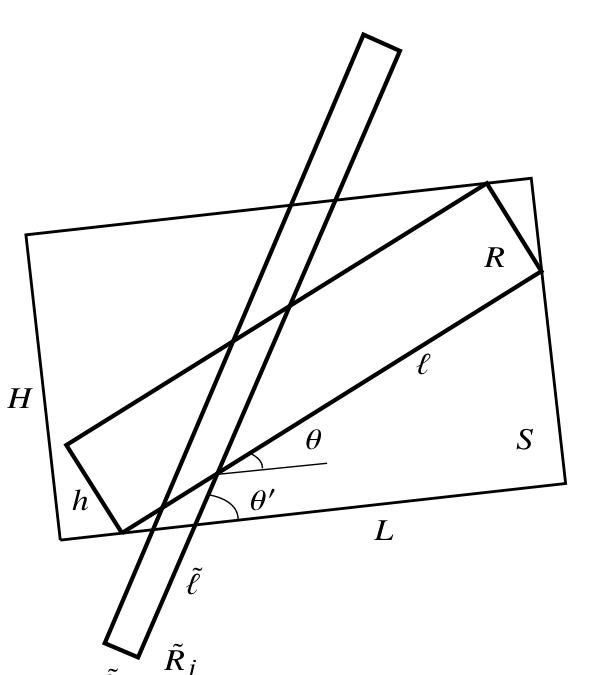
\includegraphics[width=0.38\textwidth]{figs/fig-2-6.png}
\caption{包络矩形.}
\label{fig:2.6}
\end{figure}

然后, 必要时把 $S$ 膨胀, 可以假设 $\tilde{R}_{j}$ 与 $S$ 同心. 关键在于
\begin{equation}\label{eq:2.9}
  \frac{\mu(\tilde{R}_{j}\cap S)}{\mu(S)}\geq\frac{\mu(\tilde{R}_{j}\cap R)}{\mu(R)}.
\end{equation}
事实上,
\begin{align*}
  \frac{\mu(\tilde{R}_{j}\cap S)}{\mu(S)}\sim\frac{\widetilde{h}\,H/\theta^{\prime}}{h\,L}
  =\frac{\widetilde{h}}{L\,\theta^{\prime}},\qquad
  \frac{\mu(\tilde{R}_{j}\cap R)}{|R|}\sim\frac{\widetilde{h}\,h(\theta^{\prime}-\theta)}{h\,l}
  =\frac{\widetilde{h}}{l\,(\theta^{\prime}-\theta)},
\end{align*}
而我们的不等式 \eqref{eq:2.9}, 考虑到 $l \sim L$, 为
\begin{align*}
  \frac{1}{\theta^{\prime}}\geq\frac{1}{\left(\theta^{\prime}-\theta\right)},
  \qquad\text{即}\qquad
  \theta^{\prime}-\theta\geq c\,\theta^{\prime},
\end{align*}
在我们 $\theta_k = 2^{-k}$ 的情形, 它取 $c = 1/2$ 时成立. （若 $\theta_k = (1 - \varepsilon)^k$, 则取 $c = \varepsilon$.）于是在 \eqref{eq:2.9} 中对 $j$ 求和, 有
\begin{align*}
  \frac{1}{\mu(S)}\int_{S}\sum_{\substack{\tilde{R}_{j}\ \text{在}\ R\ \text{之前}}}\chi_{\tilde{R}_{j}}
  \geq\frac{1}{\mu(R)}\int_{R}\sum_{\substack{\tilde{R}_{j}\ \text{在}\ R\ \text{之前}}}\chi_{\tilde{R}_{j}}
  \geq\frac{1}{2}\,c.
\end{align*}
换句话说, 在 $\bigcup_{j}R_{j}$ 上有
\begin{align*}
  M_{2}\Big(\sum_{j}\chi_{R_{j}}\Big)>\frac{1}{2}\,c,
\end{align*}
由 $M_{2}$ 的有界性, 并由 \eqref{eq:2.9}, 可见
\begin{align*}
  \mu\Big(\bigcup_{j}R_{j}\Big)\lesssim\Big\|\sum_{j}\chi_{\tilde{R}_{j}}\Big\|_{2}^{2}
  \lesssim\mu\Big(\bigcup_{j}\tilde{R}_{j}\Big).
\end{align*}
这里我们控制算子 $\mathcal{M}$ 于 $M_2$, 其方式与先前用 $M_{n-1}$ 控制 $M_n$ 完全一样. 而 $\mathcal{M}$ 是三参数极大算子, $M_2$ 是两参数算子.

最后应该注意, 如前, 这个覆盖引理蕴含 $\mathcal{M}$ 的极大定理, 正如所断言的那样. 事实上, 假设已经证明: 给定 $\{R_k\}$, 存在子列 $\{\tilde{R}_k\}$, 使得
\begin{align*}
  \mu\Big(\bigcup_{k}\tilde{R}_{k}\Big)\gtrsim\mu\Big(\bigcup_{k}R_{k}\Big),
\end{align*}
\begin{enumerate}
\item[(2)] $\Big\|\sum_{k}\chi_{R_k}\Big\|_{p'} \lesssim \mu\Big(\bigcup_{k} R_k\Big)^{1/p'}$, 其中 $1/p + 1/p' = 1$.
\end{enumerate}
则
\begin{align*}
  \mu(\{\mathcal{M}f>\alpha\})\leq\left(c\,\frac{\left\|f\right\|_{p}}{\alpha}\right)^{p}.
\end{align*}
事实上, 由定义存在 $\{R_{k}\}$, 使
\begin{align*}
  \{\mathcal{M}f>\alpha\}\subseteq\bigcup_{k}R_{k},\qquad
  \frac{1}{\left|R_{k}\right|}\int_{R_{k}}\left|f\right|>\alpha\quad\text{对所有 } k.
\end{align*}
由覆盖引理选取类 $\{\tilde{R}_{k}\}$. 则
\begin{align*}
  |\tilde{R}_{k}|\leq\frac{1}{\alpha}\int_{\tilde{R}_{k}}|f|,
\end{align*}
于是
\begin{align*}
  \mu\Big(\bigcup_{k}\tilde{R}_{k}\Big)
  &\leq\frac{1}{\alpha}\int f\sum_{k}\chi_{\tilde{R}_{k}}
  \leq\frac{1}{\alpha}\left\|f\right\|_{p}\left\|\sum_{k}\chi_{R_{k}}\right\|_{p^{\prime}}
  \leq\frac{C}{\alpha}\left\|f\right\|_{p}\,\mu\Big(\bigcup_{k}R_{k}\Big)^{1/p^{\prime}}\\
  &\leq C^{\prime}\left\|f\right\|_{p}\,\mu\Big(\bigcup_{k}\tilde{R}_{k}\Big)^{1/p^{\prime}},
\end{align*}
把两边除以 $\mu\bigl(\bigcup_{k}\tilde{R}_{k}\bigr)^{1/p'}$, 即得关于 $\mu(\{\mathcal{M}f > \alpha\})$ 的估计.

上述论证给出了 $\R^2$ 中一般\newterm{lacunary}{缺项的}{lacunary}\newterm{direction-set}{方向集}{set of directions}的类似定理, 即满足 $\theta_k \searrow \theta$ 且对 $k = 1, 2, 3, \ldots$
\begin{align*}
  \frac{\theta_k - \theta_{k+1}}{\theta_{k+1} - \theta_{k+2}} \geq \rho > 1
\end{align*}
的集合 $\{\theta_k\}$.

此外, 结果对一般 $p > 1$ 成立. 即, 对 $p > 1$ 有不等式
\begin{align*}
  \mu\{\mathcal{M}f>\alpha\}\leq c_{p}(\rho)\,\alpha^{-p}\|f\|_{p}^{p},
\end{align*}
见 \cite{b50}. 但那里的证明不循本章的至上主义方法.

% ================================================================
% 编号审计 (第 2 章):
%   lemma     lem:2.1  → 引理 2.1  (§2.1)
%   lemma     lem:2.2  → 引理 2.2  (§2.1)
%   lemma     lem:2.3  → 引理 2.3 (Calderón–Zygmund) (§2.1)
%   definition def:2.4 → 定义 2.4  (§2.2)
%   theorem   thm:2.5  → 定理 2.5  (§2.2)
%   remark    rem:2.6  → 注 2.6    (§2.2)
%   theorem   thm:2.7  → 定理 2.7  (§2.3)
%   theorem   thm:2.8  → 定理 2.8  (§2.4)
%   definition def:2.9 → 定义 2.9  (§2.4)
%   lemma     lem:2.10 → 引理 2.10 (§2.4)
%   theorem   thm:2.11 → 定理 2.11 (§2.4)
%   公式: eq:2.1 (Hardy–Littlewood 极大函数), eq:2.2 (弱型不等式),
%         eq:2.3 (稀疏性), eq:2.4 (指数估计), eq:2.5 (切片估计),
%         eq:2.6 (选择过程), eq:2.7 (双指数恒等式), eq:2.8 (重叠比),
%         eq:2.9 (包络矩形比)
%   无编号 Claim 用 claim* 环境 (证明内嵌于定理 2.8 的证明).
%   \cite 使用: b14 b41 b46 b48 b50 b51 b52 b54 b56 b57
% ================================================================

% ================================================================
%  第 3 章 针之所转: Besicovitch 集与 Kakeya 集
%  依据原书 PDF 第 43--62 页译出；编号审计见文件末尾注释
% ================================================================

\chapter{针之所转: Besicovitch 集与 Kakeya 集}

\epigraph{矩形并非有意识的形式. 它是直觉理性的创造. 是新生艺术的面孔. 通往纯粹创造的第一步.}{Kazimir S. Malévich}

\section{认清敌人}

若允许矩形有任意方向，则微分定理竟然是假的——即使对可测集的示性函数亦然——而相应的极大函数对 $L^p$-空间（$1 \leq p < \infty$）中的函数可以几乎处处为无穷. 文献 \cite{b46} 与 \cite{b32} 含有这些事实的证明.

J.~Littlewood 有一个有趣的评论（\cite{b69}，第 392 页）: 他说，为证明一个定理，正确的做法是先找到所要证明之物的最凶恶的敌人，然后引入恰当的假设迫使它改换阵营. Littlewood 为他的原则给出了一个极好的例子: 假设在半带形 $-\pi/2 \leq x \leq \pi/2$，$y \geq 0$ 上有一个解析函数 $F(z)$，在边界上满足 $|F(z)| \leq 1$. 在带形内部是否也有 $|F(z)| \leq 1$?

函数 $F_0(z) = \exp(e^{-iz} - 1)$ 表明答案是否定的. 另一方面，若加上条件: 对某个 $\varepsilon > 0$，$|F(z)| \leq K\exp[\exp((1 - \varepsilon)y)]$，则答案是肯定的，因为这个条件消灭了敌人，并在证明中扮演重要角色. 有趣的是，Littlewood 正是用这一哲学，于 1962 年在他所引的论文中断言: Lulin 关于傅里叶级数几乎处处收敛的猜想应当是错的——而这不过几年之后，Carleson 就给出了著名的证明!

\begin{question}\label{ques:3.1}
求一个面积最小的平面集，在其中可以连续地转动一根针并调换其两端的位置.
\end{question}

这个古怪的问题由日本数学家挂谷宗一（Soichi Kakeya）在一个多世纪前于 \cite{b71} 中提出，如今已成为当代调和分析的核心课题，并且在某种意义上，它与数学分析中最稳固的范式之一——Lebesgue 积分理论——引入了矛盾的因素.

这里的针是 $\R^2$ 中一条长为 $1$ 的有向线段 $\overrightarrow{AB}$. 我们首先想到的能把它转到位置 $\overrightarrow{BA}$ 的集合，是以其中点为心、半径 $1/2$ 的圆，面积为 $\pi/4$. 但这远非问题的解；特别地，还有另一个以星形线为边界的平面集，在其中也可以转动这根针，其面积为 $\pi/8$. 今天我们都知道，这两个集合对回答 Kakeya 的问题都无关紧要，但这一发现属于乌克兰数学家 Abram Besicovitch——几何测度论的创立者之一.

Besicovitch 所关心的是一个稍有不同的问题，为此他构造了 $\R^2$ 中一个闭的有界集，测度为 $0$，在任意方向上都含有一条单位线段. 特别地，该构造蕴含不存在面积最小的这样的集合，因为对每个 $\varepsilon > 0$，都存在面积小于 $\varepsilon$ 的平面集，在其中可以连续地转动一根针并调换两端的位置.

Besicovitch 于动荡的 1919 年在一份不太知名的俄国期刊 \cite{b58} 上发表了论文，当时他并不知道 Kakeya 提出的问题——正如他在多年后发表于 American Mathematical Monthly 的文章 \cite{b62} 中所陈述的那样. 不过，他的动机是不同的，与对 Fubini 定理的理解有关: 该定理对 Lebesgue 积分成立，但对 Riemann 积分方法一般不成立. 不难找到 $\R^2$ 中的函数 $f$，它是 Riemann 可积的（即其不连续点集在 $\R^2$ 中测度为 $0$），但对某个特定值，函数 $x \to f(x, y_0)$ 不是 Riemann 可积的，因为其不连续点集在实直线上有正测度.

一个例子是定义在单位正方形 $Q$ 上的函数 $f$:
\begin{align*}
  f(x,y)=\begin{cases}
  1, & \text{若 } y\neq y_{0},\ \text{其中 } 0<y_{0}<1 \text{ 固定},\\
  1, & \text{若 } y=y_{0} \text{ 且 } x \text{ 为无理数},\\
  0, & \text{若 } y=y_{0} \text{ 且 } x \text{ 为有理数}.
  \end{cases}
\end{align*}
则二重积分 $\iint_{Q} f(x,y) \,\mathrm{d}x\,\mathrm{d}y = 1$ 存在，但 $\int_{0}^{1} \bigl(\int_{0}^{1} f(x,y) \,\mathrm{d}x\bigr) \mathrm{d}y$ 没有意义，因为 $f(x,y_0)$ 不是 Riemann 可积的.

然而，在这个例子中，如果我们足够聪明地旋转坐标轴，困难就消失了.

于是出现下面的问题: 给定 $\R^2$ 中的 Riemann 可积函数，能否选择适当的坐标轴，使二重积分等于累次积分?

Besicovitch 构造的集合给出了否定的回答，而且按照 Littlewood 的说法，它也正是当我们在平面上考虑任意方向矩形上的平均时，Lebesgue 微分定理不成立的主要敌人.

\begin{theorem}\label{thm:3.2}
对每个 $0 < \varepsilon < 1$，存在紧平面集 $K_\varepsilon$，在任意方向上都含有一个 $\varepsilon \times 1$ 的矩形，且其 Lebesgue 测度 $\mu(K_\varepsilon)$ 以 $C/(1 + |\log \varepsilon|)$ 为上界，其中 $C < \infty$ 是普适常数.
\end{theorem}

\begin{proof}
(a) 基本构造. 从一个底边长 $b_0$、高 $h_0$ 的三角形 $T_0$ 出发，用过其底边中点的中线把它分成两个小三角形: $T_0 = T_0^1 \cup T_0^2$.

\begin{center}
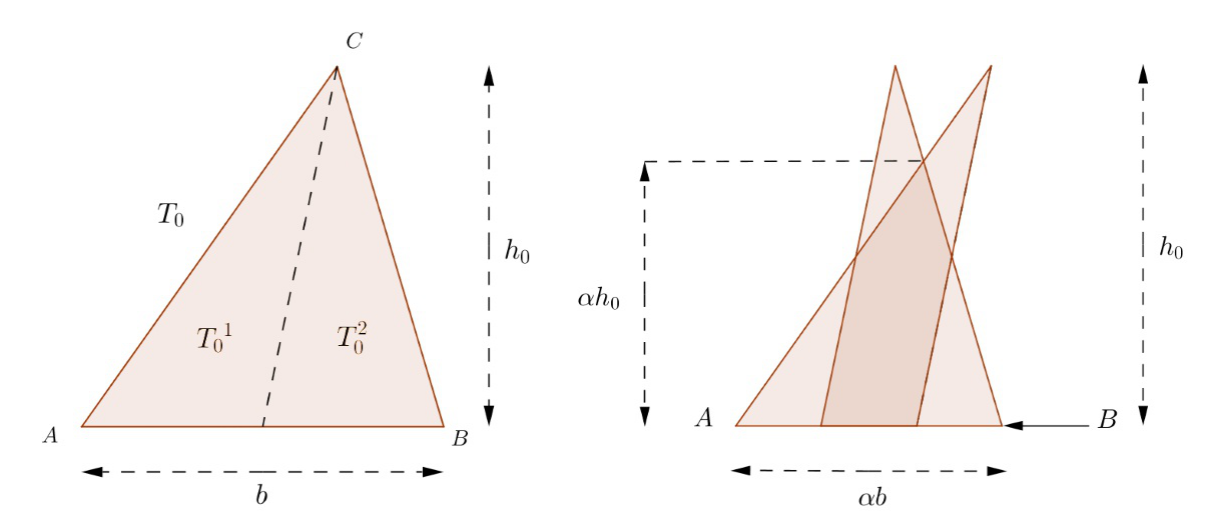
\includegraphics[width=0.6\textwidth]{figs/fig-3-1a.png}
\end{center}

接着，以因子 $\alpha$（$1/2 < \alpha < 1$）平移 $T_0^1$ 与 $T_0^2$，使它们的底边重叠，产生一个图形 $A_1$（树），它由一个与 $T_0$ 相似、比例为 $\alpha$ 的三角形 $T_1$（树干）以及若干树枝 $B_1$ 组成，树枝是与 $T_0^1$ 或 $T_0^2$ 相似、比例为 $1 - \alpha$ 的四个三角形之并.

一个初等计算给出
\begin{align*}
  \mu(A_{1})=\mu(T_{1})+\mu(B_{1})=\bigl(\alpha^{2}+2(1-\alpha)^{2}\bigr)\mu(T_{0})<\mu(T_{0})
\end{align*}
对任何 $1/2 < \alpha < 1$ 成立.

(b) 想法是把基本构造迭代许多次. 现在从高 $h_0$ 的等边三角形 $T_0$ 出发，把其长为 $b_0$ 的底边分成 $2^n$ 个等长 $b_0\,2^{-n}$ 的线段，并把 $T_0$ 分解成 $2^n$ 个小三角形 $T_0^j$，$j = 1, \ldots, 2^n$.

然后对每对 $(T_0^{2k-1}, T_0^{2k})$（$k=1,\ldots,2^{n-1}$），用待定的参数 $\alpha_1$（$1/2<\alpha_1<1$）构造树 $A_1^k=T_1^k\cup B_1^k$，并注意到这些相邻三角形 $T_1^k, T_1^{k+1}$ 中总有两个有两条平行边（不同于它们的底边）. 因此，可以把它们全部平移得到一个新的三角形 $T_1$，与 $T_0$ 相似，底与高分别为 $\alpha_1 b_0$ 与 $\alpha_1 h_0$. 我们还相应地平移各树枝 $B_1^k$，使每个原三角形 $T_0^k$ 在平移后都包含于所得的树 $A_1=T_1\cup\{\text{平移后的树枝}\}$ 中，如上图所示.

\begin{center}
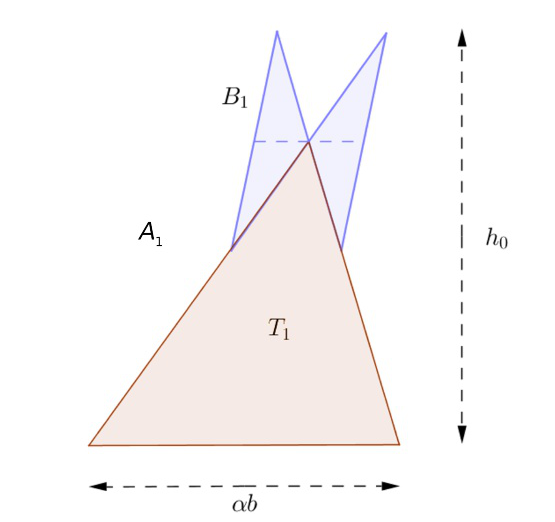
\includegraphics[width=0.36\textwidth]{figs/fig-3-1b.png}
\end{center}

\begin{figure}[htbp]
\centering
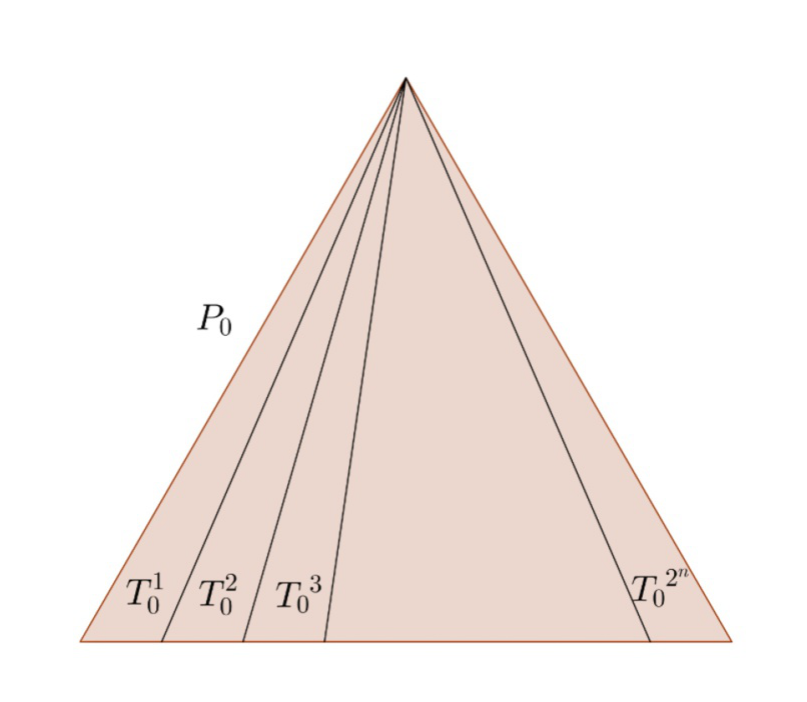
\includegraphics[width=0.5\textwidth]{figs/fig-3-1.png}
\caption{三角形细分.}
\label{fig:3.1}
\end{figure}

我们有
\begin{align*}
  \mu(A_{1})\leq\mu(T_{1})+\mu(B_{1})\leq\{\alpha_{1}^{2}+2(1-\alpha_{1})^{2}\}\mu(T_{0}).
\end{align*}

\begin{figure}[htbp]
\centering
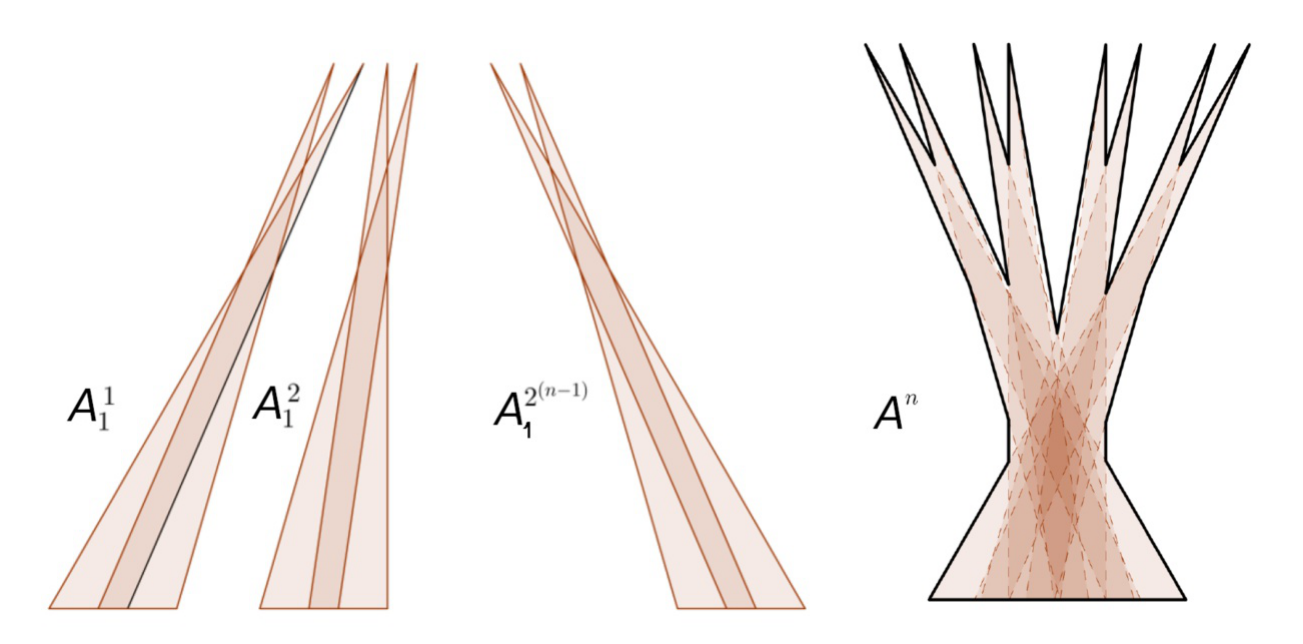
\includegraphics[width=0.66\textwidth]{figs/fig-3-2.png}
\caption{Besicovitch 配对.}
\label{fig:3.2}
\end{figure}

现在注意到 $T_1$ 是 $2^{n-1}$ 个三角形的并，它们的高相等，底长分别为 $\alpha_1 2^{-n+1} b_0$ 与 $\alpha_1 h_0$. 于是可以用另一个比例 $\alpha_2$（$1/2 < \alpha_2 < 1$）重复这一构造，得到第二棵树 $A_2 = T_2 \cup \{\text{树枝}\}$，满足
\begin{align*}
  \mu(A_{2})\leq\left[\alpha_{1}^{2}\alpha_{2}^{2}+2\bigl((1-\alpha_{1})^{2}+\alpha_{1}^{2}(1-\alpha_{2})^{2}\bigr)\right]\mu(T_{0}),
\end{align*}
如此等等.

把这一过程迭代 $n$ 次，产生一棵树 $A_{n}$，使
\begin{align*}
  \mu(A_{n})\leq\{\alpha_{1}^{2}\alpha_{2}^{2}\cdots\alpha_{n}^{2}
  +2[(1-\alpha_{1})^{2}+\cdots+\alpha_{1}^{2}\cdots\alpha_{n-1}^{2}(1-\alpha_{n})^{2}]\}\mu(T_{0}),
\end{align*}
且具有如下性质: 每个原三角形 $T_{0}^{k}$ 都可以平移到 $A_{n}$ 之内.

选取
\begin{align*}
  \alpha_{k}=1-\frac{1}{n+2-k}=\frac{n+1-k}{n+2-k},\qquad k=1,2,\ldots,n,
\end{align*}
给出估计
\begin{align*}
  \mu(A_{n})\leq\frac{2}{n+1}\mu(T_{0}).
\end{align*}
若现在以 $h_0 = 2$ 出发，则集合 $A_n$ 与其按角 $\pi j/3$（$j = 1, 2, 3, 4, 5$）的旋转之并，在适当选取 $n$（即 $2^{-n} \sim \varepsilon$）时给出集合 $K_\varepsilon$.
\end{proof}

显然，在 $K_{\varepsilon}$ 内部，每个平面方向上都放得下一根针. 不过，给 $K_{\varepsilon}$ 添上测度任意小的集合后，我们还能在集合内部连续地移动这根针. 原因是 $K_{\varepsilon}$ 是一些三角形的并，这些三角形的最长边可以成对安排成具有相同的方向，而我们总可以付出任意小的面积，把一条线段在两条平行线之间平移，如下图所示:

\begin{center}
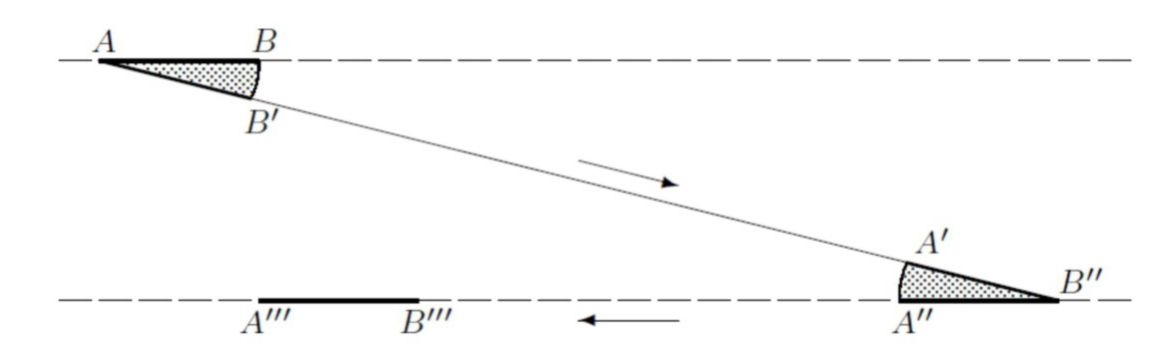
\includegraphics[width=0.55\textwidth]{figs/fig-3-kappa.png}
\end{center}

虚线区域可以做到面积任意小: 只要把平移做得足够远，再利用一条线段在一条直线内移动时产生零面积这一事实即可.

因此，如前所指出的，Kakeya 的原始问题有如下答案: 不存在面积最小的这样的集合，因为对每个 $\varepsilon > 0$，都存在面积小于 $\varepsilon$ 的平面区域，在其中可以转动这根针.

Besicovitch 构造是最优的，如下面的定理所示.

\begin{theorem}\label{thm:3.3}
存在有效常数 $C > 0$，使得若一个平面集在每个方向上都含有一个 $\varepsilon \times 1$ 的矩形（$0 < \varepsilon < 1$），则其面积必大于 $C/[1 + |\log \varepsilon|]$.
\end{theorem}

\begin{proof}
设 $A$ 是这样的集合. 对每个 $j$，$0 \leq j \leq \varepsilon^{-1}$，设 $R_j \subset A$ 是方向（即其最长边的方向）为 $\omega_j = \tfrac{1}{2}\pi\varepsilon j$ 的 $\varepsilon \times 1$ 矩形. Hölder 不等式给出
\begin{align*}
  1\leq\sum_{j}\mu(R_{j})=\int\sum_{j}\chi_{R_{j}}
  \leq\left[\mu\Big(\bigcup_{j}R_{j}\Big)\right]^{1/2}\Big[\sum_{j,k}\mu(R_{j}\cap R_{k})\Big]^{1/2}.
\end{align*}
一个直接的三角计算给出估计
\begin{align*}
  1\leq\left[\mu(A)\right]^{1/2}\Big[\sum_{j,k=1}^{\varepsilon^{-1}}\frac{\varepsilon}{\left|j-k\right|+1}\Big]^{1/2},
\end{align*}
即 $\mu(A) \gtrsim (1 + |\log \varepsilon|)^{-1}$.
\end{proof}

下面我们将修改 Besicovitch 构造，以得到一个极限集 $K$.

\begin{theorem}\label{thm:3.4}
存在测度 $\mu(K) = 0$ 的紧集 $K \subset \R^2$，在每个平面方向上都包含一条单位线段.
\end{theorem}

\begin{proof}
从边长为 $2$ 的等边三角形出发，把其底边分成 $2^{n_0}$ 等份，其中 $n_0$ 取得足够大，使得当我们用参数 $\alpha = 2/3$ 对相邻三角形 $T_0^{2j-1}$，$T_0^{2j}$（$j = 1, \ldots, 2^{n_0-1}$）应用 Besicovitch 的基本构造时，相应的树枝都位于直线 $y = 1$ 上方的区域之内.

我们可以自由地把 $T_0^{2j-1}$ 朝 $T_0^{2j}$ 的方向移动，反之亦然，只有两个极端除外；也就是说，我们希望线段 $AA'BB'$ 包含于所得的三角形 $T_1^1, T_1^2, \ldots, T_1^{2^{n_0}-1}$ 中，从而包含于一族菱形
\begin{align*}
  R_{1}^{\nu_{1}}=T_{1}^{\nu_{1}}\cap\{0\leq y\leq 1\},\qquad \nu_{1}=1,\ldots,2^{n_{0}-1}
\end{align*}
之中. 注意，集合 $\bigcup_{\nu_1} R_1^{\nu_1}$ 在原来三角形的每个方向（即由顶点 $C$ 处的角给出的方向集 $\Gamma$）上都含有一条长度为 $1$ 的直线段，并满足估计
\begin{align*}
  \mu\Big(\bigcup_{\nu_{1}}R_{1}^{\nu_{1}}\Big)\leq\frac{2}{3}\,\mu(R_{0}),
\end{align*}
其中 $R_{0}$ 是以 $AA^{\prime}BB^{\prime}$ 为顶点的菱形.

接着对每个三角形 $T_1^{\nu_1}$ 应用同一过程，得到另一族菱形 $\{R_2^{\nu_1, \nu_2}\}$，使得:
\begin{enumerate}
\item[(i)] $\mu\bigl(\bigcup_{\nu_1, \nu_2} R_2^{\nu_1, \nu_2}\bigr) \leq \bigl(\tfrac{2}{3}\bigr)^2 \mu(R_0)$；
\item[(ii)] 一条长度 $1$、方向属于顶点 $C$ 处原角 $\widehat{ACB}$ 的线段可以放入 $\bigcup_{\nu_1, \nu_2} R_{2}^{\nu_1, \nu_2}$ 之内；
\item[(iii)] $\bigcup_{\nu_1,\nu_2} R_2^{\nu_1,\nu_2}$ 包含所有菱形 $\{R_1^{\nu_1}\}$ 的侧边界线段.
\end{enumerate}
迭代这一过程，对每个 $j = 1,2,\ldots$ 得到一族闭菱形 $\{R_j^{\nu_1,\ldots,\nu_j}\}$ 与一个紧集 $K_j = \bigcup_{\nu_1,\ldots,\nu_j} R_j^{\nu_1,\ldots,\nu_j}$，使得:
\begin{enumerate}
\item[(iv)] $\mu(K_j) \leq \bigl(\tfrac{2}{3}\bigr)^j \mu(R_0)$；
\item[(v)] $K_{j}$ 在原始方向集 $\Gamma$ 的每个方向上都含有一条长度为 $1$ 的线段；
\item[(vi)] 存在稠密的方向集 $\{\theta_e\} \subset \Gamma$，使得对每个 $j = 1, 2, \ldots$，都能在所有的 $K_j$ 中找到一条方向为 $\theta_e$ 的直线段 $I_{\theta_e}$.
\end{enumerate}
令 $K = \bigcap_j K_j$. 则 $K$ 紧，$\mu(K) = 0$，且对每个 $\theta \in \Gamma$，存在一列收敛到 $\theta$ 的上述 $\theta_e$，从而相应的线段 $I_{\theta_e}$ 必收敛到一条方向为 $\theta$ 的线段 $I_\theta$，而由紧性，它也必须包含于集合 $K$ 中.
\end{proof}

\begin{definition}\label{def:3.5}
平面中的\newterm{besicovitch-set}{Besicovitch 集}{Besicovitch set}（或\newterm{kakeya-set}{Kakeya 集}{Kakeya set}）是测度为 $0$、在每个方向上都含有一条定长直线段的集合.
\end{definition}

\begin{corollary}\label{cor:3.6}
平面中 Besicovitch 集的 Minkowski 维数（计盒维数）为 $2$.
\end{corollary}

\begin{proof}
不失一般性，可设 $K$ 在每个方向上都含有长度为 $1$ 的线段. 对每个 $\varepsilon > 0$，集合 $K_{\varepsilon} = \{x : \dist(x, K) \leq \varepsilon\}$ 在每个平面方向上都含有 $\varepsilon \times 1$ 的矩形. 于是
\begin{align*}
  \mu(K_{\varepsilon})\geq\frac{1}{1+|\log\varepsilon|},\qquad
  \lim_{\varepsilon\to 0}\left[2-\frac{\log\mu(K_{\varepsilon})}{\log\varepsilon}\right]=2.
\end{align*}
\end{proof}

\section{Kakeya 极大函数}

设 $N \gg 1$，$\rho > 0$，考虑 $\R^2$ 中所有尺寸为 $\rho \times \rho N$、方向任意的平面矩形组成的族 $\mathcal{B}_N^\rho$. 给定 $\R^2$ 中的局部可积函数 $f$，有极大算子
\begin{align*}
  M_{N}^{\rho}f(x)=\sup_{x\in R\in\mathcal{B}_{N}^{\rho}}\frac{1}{\mu(R)}\int_{R}\left|f(y)\right|\,\mathrm{d}\mu(y).
\end{align*}

\begin{theorem}\label{thm:3.7}
存在有限常数 $C$（与 $N$ 和 $\rho$ 无关），使得对每个 $f \in L^2(\R^2)$ 下列估计成立:
\begin{align*}
  \left\|M_{N}^{\rho}f\right\|_{2}\leq C\left[\log(1+N)\right]^{1/2}\left\|f\right\|_{2}.
\end{align*}
\end{theorem}

\begin{remark}\label{rem:3.8}
只需证明 $\rho = 1$ 的情形，一个方便的膨胀论证即可说明这一点. 由于每个 $R \in \mathcal{B}_N^1$ 都包含于边长为 $N$ 的正方形中，可知 $M_N^1 f(x) \leq N \cdot M f(x)$，其中 $M$ 表示 Hardy--Littlewood 极大函数. 因此，定理的要点不是 $M_N^\rho$ 的有界性，而是其范数的估计 $(\log N)^{1/2}$.
\end{remark}

\begin{proof}[定理~\ref{thm:3.7} 的证明]
族 $\mathcal{B}_N^1$ 可以按其中矩形的方向 $\theta$ 分成两个子族 $\mathcal{B}_{N,1}^1 \cup \mathcal{B}_{N,2}^1$: 对 $\mathcal{B}_{N,1}^1$，$\theta \in [-\pi/4, \pi/4]$；对 $\mathcal{B}_{N,2}^1$，$\theta \in [\pi/4, 3\pi/4]$.

显然，$\mathcal{B}_{N,1}^{1}$ 与 $\mathcal{B}_{N,2}^{1}$ 的相伴极大函数有相同的界. 因此，只须考虑其中之一.

设 $\R^2 = \bigcup_{\nu \in \Z^2} Q_\nu$ 是平面被分成面积 $1$、边平行于坐标轴的不交正方形网格的标准分解.

给定 $f \in L^2(\R^2)$，对每个 $\nu$ 选取矩形 $R_\nu \in \mathcal{B}_{N,1}^1$，满足 $Q_\nu \cap R_\nu \neq \emptyset$ 且
\begin{align*}
  \sup_{x\in Q_{\nu}}M_{N,1}^{1}f(x)\leq 2\,\frac{1}{\mu(R_{\nu})}\int_{R_{\nu}}\left|f(y)\right|\,\mathrm{d}\mu(y),
\end{align*}
即
\begin{align*}
  M_{N,1}^{1}f(x)\leq 2\sum_{\nu}\Big(\frac{1}{N}\int_{R_{\nu}}|f(y)|\,\mathrm{d}\mu(y)\Big)\cdot\chi_{Q_{\nu}}(x).
\end{align*}
于是我们的估计将是下面结果的推论.

\begin{lemma}\label{lem:3.9}
存在有限常数 $C$（与 $N$ 无关），使得对满足 $R_\nu \cap Q_\nu \neq \emptyset$ 的任何矩形 $R_\nu \in \mathcal{B}_{N,1}^1$ 的选取，由公式
\begin{align*}
  T f(x)=\sum_{\nu}\left(\frac{1}{\mu(R_{\nu})}\int_{R_{\nu}}f(y)\,\mathrm{d}y\right)\chi_{Q_{\nu}}(x)
\end{align*}
定义的算子满足估计
\begin{align*}
  \left\|T f\right\|_{2}\leq C\left[1+\log N\right]^{1/2}\left\|f\right\|_{2},\qquad f\in L^{2}(\R^{2}).
\end{align*}
\end{lemma}

\begin{proof}
为证明引理，考虑伴随算子
\begin{align*}
  T^{*}g(x)=\sum_{\nu}\left(\frac{1}{N}\int_{Q_{\nu}}g(y)\,\mathrm{d}y\right)\chi_{R_{\nu}}(x)
\end{align*}
是方便的，并注意到，由于所涉矩形的尺寸是 $1 \times N$，只须检验 $T^*$ 在支于 $N \times N$ 正方形上的函数上的作用.

设 $Q$ 是这样的 $N \times N$ 正方形，边平行于坐标轴. 则 $Q = E_1 \cup \cdots \cup E_N$，其中每个 $E_j$（$j = 1, \ldots, N$）是厚度 $1$ 的竖直带. 对每个 $g \in L^2(Q)$，有 $g = \sum_{j=1}^N g \cdot \chi_{E_j}$，而引理将是估计
\begin{align*}
  \|T^{*}(g\cdot\chi_{E_j})\|_{2}\lesssim N^{-1/2}\left(\log N\right)^{1/2}\|g\cdot\chi_{E_{j}}\|_{2}
\end{align*}
的推论. 为看出这一点，进一步分解 $E_j = \bigcup_{i=1}^{N} Q_i$，其中正方形 $Q_i$ 属于初始网格 $\{Q_\nu\}$，指标 $i$ 表示竖直方向的位置. 再设 $R_i$ 是算子 $T$ 定义中相应指派的 $\mathcal{B}_{N,1}^1$ 矩形. 则
\begin{align*}
  \int|T^{*}(g\cdot\chi_{E_{j}})(x)|^{2}\,\mathrm{d}x
  &\lesssim\sum_{i,k=1}^{N}\frac{1}{N^{2}}\Big(\int_{Q_{i}}|g|^{2}\Big)^{1/2}\Big(\int_{Q_{k}}|g|^{2}\Big)^{1/2}\frac{N}{|i-k|+1}\\
  &\lesssim\frac{1}{N}\left(1+\log N\right)\|g\cdot\chi_{E_{j}}\|_{2}^{2}.
\end{align*}
\end{proof}

\end{proof}

定理 3.7 容许如下的改进: 给定 $N \gg 1$，用 $\mathcal{B}_N$ 表示 $\R^2$ 中离心率（两边长之比）等于 $N$、方向任意的矩形类. 再考虑相伴的极大函数:
\begin{align*}
  M_N f(x)=\sup_{x\in R\in\mathcal{B}_{N}}\frac{1}{\mu(R)}\int_{R}\left|f(y)\right|\,\mathrm{d}\mu(y),
\end{align*}
定义于局部可积函数 $f$ 之上.

\begin{theorem}\label{thm:3.10}
存在有限正常数 $C$ 与 $a$，使得
\begin{align*}
  \left\|M_{N}f\right\|_{2}\leq C(\log N)^{a}\left\|f\right\|_{2}
\end{align*}
对每个函数 $f\in L^{2}(\R^{2})$ 成立.
\end{theorem}

\begin{proof}
首先注意，给定离心率为 $N$ 的任何矩形 $R$，都能找到尺寸相同、方向属于角集 $\{\pi k N^{-1}\}_{k=1,\ldots,N}$ 的另一矩形 $\tilde{R}$，使 $R$ 包含于二倍矩形 $(\tilde{R})^*$ 中. 由此可知，不失一般性，只须对这样的受限方向集 $\{\pi k N^{-1}\}_{k=1,\ldots,N}$ 中的矩形证明上述陈述即可.

用类似的论证，我们还可以假定较短的边长具有形式 $2^n$，$n \in \Z$.

接下来引入如下记号:
\begin{align*}
  T_{2^{n}}^{j}f(x)=\sup_{x\in R}\frac{1}{\mu(R)}\int_{R}\left|f(y)\right|\,\mathrm{d}\mu(y),
\end{align*}
其中上确界取遍所有尺寸为 $2^n \times 2^n N$、方向为 $\pi j N^{-1}$ 的矩形；以及
\begin{align*}
  T_{2^{n}}=\sup_{j}T_{2^{n}}^{j},\qquad
  T^{j}=\sup_{n}T_{2^{n}}^{j},\qquad
  T=\sup_{j}T^{j}=\sup_{n}T_{2^{n}}.
\end{align*}
给定 $\alpha > 0$，可以对每个 $j$ 应用标准（Vitali）覆盖引理，得到一列方向为 $\pi j N^{-1}$、两两不交的矩形 $\{R_l^j\}_{l=1,2,\ldots}$，使得
\begin{align*}
  E_{\alpha}^{j}=\{x:T^{j}f(x)\geq\alpha\}\subset\bigcup_{l}(R_{l}^{j})^{*},\qquad
  \frac{1}{\mu(R_{l}^{j})}\int_{R_{l}^{j}}|f(y)|\,\mathrm{d}\mu(y)\geq\alpha.
\end{align*}
于是，由前述评注，我们知道
\begin{align*}
  E_{\alpha}=\{x:M_{N}f(x)\geq 4\alpha\}\subset\bigcup_{j=1}^{N}E_{\alpha}^{j}.
\end{align*}
设 $n_0$ 是存在尺寸为 $2^{n_0} \times 2^{n_0} N$ 的矩形属于上述序列之一的最大整数，并考虑所有这些矩形组成的族. 我们可以选出具有如下性质的子族 $F_0$: $F_0$ 中没有矩形包含于另一个的二倍矩形之内，而被淘汰的矩形必包含于 $F_0$ 中某个成员的二倍矩形之内.

由归纳，对每个 $k$ 得到一族尺寸为 $2^{n_k} \times 2^{n_k} N$（$n_0 > n_1 > \cdots$）的矩形 $\mathcal{F}_k$，使得 $\mathcal{F}_k$ 中没有矩形包含于 $\mathcal{F}_j$（$j \leq k$）中另一个矩形的二倍矩形之内，且若 $R$ 属于原始的 $N$-族，则 $R$ 要么属于某个 $\mathcal{F}_k$，要么包含于 $\bigcup_k \mathcal{F}_k$ 中某个成员的二倍矩形之内.

由此得
\begin{align*}
  E_{\alpha}\subset\bigcup_{R\in\bigcup_{k}\mathcal{F}_{k}}(R^{*})^{*}.
\end{align*}

接着，对 $k = 0, 1, 2, \ldots$ 定义
\begin{align*}
  \Delta_{k}&=\left\{R\in\bigcup_{j}\mathcal{F}_{j}:\dim(R)=2^{n}\times 2^{n} N;\ n_{0}-k\log N\geq n\geq n_{0}-(k+1)\log N\right\},\\
  E_{i}&=\bigcup_{R\in\Delta_{i}}R,\qquad
  E_{i}^{**}=\bigcup_{R\in\Delta_{i}}\left(R^{*}\right)^{*}.
\end{align*}
注意，集合族 $\{E_i\}$ 是``几乎不交''的，即若 $|i - j| \geq 2$ 则 $E_i \cap E_j = \emptyset$. 这是因为若 $R_1 \in \Delta_i$，$R_2 \in \Delta_j$ 且 $i - j \geq 2$，则 $R_2$ 的最长边小于 $R_1$ 的最短边；又若 $R_1 \cap R_2 \neq \emptyset$，则 $R_2$ 包含于 $R_1^*$，这与我们选取序列 $\mathcal{F}_k$ 的方式矛盾.

令 $f_i = f/E_i$，$i = 0, 1, \ldots$，并设 $S_i$ 是由
\begin{align*}
  S_{i}f(x)=\sup_{x\in R}\frac{1}{\mu(R)}\int_{R}\left|f(y)\right|\,\mathrm{d}y
\end{align*}
定义的极大函数，其中上确界取遍尺寸为 $2^n \times 2^n N$ 的矩形，且
\begin{align*}
  n_{0}+2-i\log N\geq n\geq n_{0}+2-\left(i+1\right)\log N.
\end{align*}
由定理 3.7，我们知道 $S_i$ 在 $L^2(\R^2)$ 上有界，且其范数以 $C(\log N)^{3/2}$ 为界，其中 $C$ 与 $N$ 和 $i$ 无关.

给定 $x \in E_i^{**}$，存在 $R \in \Delta_i$ 使 $x \in (R^*)^*$，从而
\begin{align*}
  S_{i}\,f_{i}(x)\geq\frac{1}{16}\frac{1}{\mu(R)}\int_{R}\left|f_{i}(y)\right|\,\mathrm{d}\mu(y)\geq\frac{\alpha}{16},
\end{align*}
即
\begin{align*}
  E_{i}^{**}\subset\{x:S_{i}f_{i}(x)\geq\alpha/16\},\qquad
  \mu(E_{i}^{**})\lesssim(\log N)^{3}\frac{\|f_{i}\|_{2}^{2}}{\alpha^{2}},
\end{align*}
\begin{align*}
  \mu(E_\alpha)
  &\leq\sum_{i}\mu(E_{i}^{**})
  \lesssim(\log N)^{3}\frac{1}{\alpha^{2}}\int f(x)^{2}\sum_{i}\chi_{E_{i}}(x)\,\mathrm{d}\mu(x)
  \lesssim(\log N)^{3}\frac{1}{\alpha^{2}}\|f\|_{2}^{2},
\end{align*}
即 $M_N$ 满足界为 $\lesssim (\log N)^3$ 的弱 $L^2$ 估计.

由于 $M_N$ 在 $L^\infty$ 上有界且满足界为 $N$ 的弱 $L^1$ 不等式，直接应用 Marcinkiewicz 与 Riesz--Thorin 插值定理即得定理中的强 $L^2$-估计.
\end{proof}

\section{Kakeya 集的 Hausdorff 维数}

给定 Borel 集 $E \subset \R^n$ 以及 $\alpha \geq 0$，$\delta > 0$，定义
\begin{align*}
  H_{\delta}^{\alpha}(E):=\inf\sum[\diam\left(B_{k}\right)]^{\alpha},
\end{align*}
其中下确界取遍 $E$ 的一切由直径小于 $\delta$ 的方体组成的可数覆盖. 再定义
\begin{align*}
  H^{\alpha}(E):=\lim_{\delta\rightarrow 0}H^{\alpha}_{\delta}(E).
\end{align*}
这个极限总是存在，尽管可能为无穷，且具有若干基本性质:
\begin{enumerate}
\item[(1)] $H^\alpha$ 是可数可加的，在平移与旋转下不变，且对 $\lambda > 0$ 满足 $H^\alpha(\lambda E) = \lambda^\alpha H^\alpha(E)$；
\item[(2)] $H^0(E)$ 计数 $E$ 中的点数，而对一切 Borel 集 $E \subset \R^n$，$H^n(E) = c_n \mu(E)$，其中
\begin{align*}
  c_{n}=\frac{\pi^{n/2}}{2^{n}\left(n/2\right)!};
\end{align*}
\item[(3)] 若 $H^{\alpha}(E) < \infty$ 且 $\beta > \alpha$，则 $H^{\beta}(E) = 0$. 若 $\beta < \alpha$ 且 $H^{\alpha}(E) > 0$，则 $H^{\beta}(E) = \infty$.
\end{enumerate}
因此，给定 Borel 集 $E \subset \R^n$，存在唯一的 $\alpha$，使 $\beta > \alpha$ 时 $H^\beta(E) = 0$，$\beta < \alpha$ 时 $H^\beta(E) = \infty$.

\begin{definition}\label{def:3.11}
这个唯一的 $\alpha$ 称为 $E$ 的\newterm{hausdorff-dimension}{Hausdorff 维数}{Hausdorff dimension}. 即
\begin{align*}
  \dim_{H}(E)=\sup\{\beta:H^{\beta}(E)=\infty\}=\inf\{\alpha:H^{\alpha}(E)=0\}.
\end{align*}
\end{definition}

若 Borel 集 $E \subset \R^n$ 有正 Lebesgue 测度，则 $\dim_H(E) = n$.

一个有趣的观察是: 在上述定义中，可以用球或二进方体代替方体，而不改变 $\dim_{H}(E)$ 的值. 而 Minkowski 维数（计盒维数）一般大于 Hausdorff 维数.

\begin{theorem}\label{thm:3.12}
$\R^2$ 中每个 Besicovitch（或 Kakeya）集 $K$ 都满足 $\dim_H(K) = 2$.
\end{theorem}

\begin{proof}
设 $\{Q_\nu\}$ 是由边长 $\ell(Q_\nu) \leq 2^{-k_0}$ 的二进方体组成的 $K$ 的覆盖:
\begin{align*}
  K\subset\bigcup_{\nu}Q_{\nu}=\bigcup_{k=k_{0}}^{\infty}\Big(\bigcup_{\nu}Q_{\nu}^{k}\Big),\qquad
  \text{其中 } \ell(Q_{\nu}^{k})=2^{-k}.
\end{align*}
引入如下记号:
\begin{align*}
  E^{k}=\bigcup_{\nu}Q_{\nu}^{k},\qquad
  N_{k}=\operatorname{Card}\{Q_{\nu}^{k}\}=\text{覆盖中边长为 } 2^{-k} \text{ 的方体数}.
\end{align*}
于是由定义，需要证明
\begin{align*}
  \sum_{k\geq k_{0}}N_{k}2^{-k\alpha}\geq c_{\alpha}>0,\qquad \alpha<2.
\end{align*}
事实上，尝试更强的结论是方便的，即:

\begin{claim*}
对每个 $\alpha < 2$，存在 $k \geq k_0$，使 $N_k 2^{-k\alpha} \geq c_\alpha > 0$.
\end{claim*}

由于 $K$ 是 Besicovitch 集，它对每个方向 $\theta \in S^1$ 都含有长度为 $1$ 的线段 $L_\theta$. 因此
\begin{align*}
  1=\ell(L_{\theta})\leq\sum_{k\geq k_{0}}\ell(L_{\theta}\cap E^{k}).
\end{align*}
于是对每个 $\beta > 0$，存在 $C_{\beta} > 0$ 与 $k \geq k_{0}$，使
\begin{align*}
  \ell(L_{\theta}\cap E^{k})\geq C_{\beta}2^{-k\beta}.
\end{align*}
（这之所以成立，是因为否则将存在 $\beta > 0$，使得对一切 $C_\beta > 0$,
\begin{align*}
  1\leq\sum_{k\geq k_{0}}\ell(L_{\theta}\cap E^{k})\leq C_{\beta}\frac{2^{-k_{0}\beta}}{1-2^{-\beta}},
\end{align*}
而这对足够小的 $C_{\beta}$ 显然不成立.）

给定 $\beta > 0$ 及其相应的 $C_{\beta} > 0$，考虑集合
\begin{align*}
  \Gamma_{k}=\{\theta\in S^{1}:\ell(L_{\theta}\cap E^{k})\geq C_{\beta}2^{-k\beta}\}.
\end{align*}
由此得
\begin{align*}
  1\leq\mu(S^{1})\leq\sum_{k\geq k_{0}}\mu(\Gamma_{k}),
\end{align*}
因为每个角 $\theta \in S^1$ 至少有一个 $k \geq k_0$ 满足
\begin{align*}
  \ell(L_{\theta}\cap E^{k})\geq C_{\beta}2^{-k\beta}.
\end{align*}
于是存在 $k \geq k_0$，使 $\mu(\Gamma_k) \geq C_\beta 2^{-k\beta}$（理由与前面相同: 否则将有不等式
\begin{align*}
  1\leq c_{\beta}\sum_{k\geq k_{0}}2^{-k\beta}=C_{\beta}\frac{2^{-k_{0}\beta}}{1-2^{-\beta}},
\end{align*}
它对足够小的 $C_{\beta}$ 不成立）.

因此，可以在 $\Gamma_k$ 内选取至少 $\frac{1}{2}\,C_\beta\,2^{k(1-\beta)}$ 个不同的角 $\{\theta_j\}$，使得 $j \neq i$ 时 $|\theta_j - \theta_i| \geq 2^{-k}$.

然后考虑这些选定方向的相应线段 $L_{\theta_j}$，并给每条线段配一个方向为 $\theta_j$、尺寸为 $2^{-k} \times 1$ 的矩形 $R_j$. 有下列不等式:
\begin{align*}
  \sum_{j}\mu(R_{j})\geq 2^{-k}\cdot\frac{1}{2}\,C_{\beta}2^{k(1-\beta)}=\frac{1}{2}\,C_{\beta}2^{-k\beta},
\end{align*}
以及
\begin{align*}
  \sum_{j}\mu(R_{j})
  &=\int_{\bigcup_{j}R_{j}}\sum_{j}\chi_{R_{j}}(x)\,\mathrm{d}x
  \leq\mu\Big(\bigcup_{j}R_{j}\Big)^{1/2}\Big[\sum_{j,i}\mu(R_{i}\cap R_{j})\Big]^{1/2}\\
  &\lesssim\mu\Big(\bigcup_{j}R_{j}\Big)^{1/2}
   \Big[\sum_{j,i}\frac{2^{-k}}{|j-i|+1}\Big]^{1/2}
  \lesssim\mu\Big(\bigcup_{j}R_{j}\Big)^{1/2}
   \Big|\log\Big(\tfrac{1}{2}C_\beta 2^{k(1-\beta)}\Big)\Big|^{1/2}.
\end{align*}
即
\begin{equation}\label{eq:3.1}
  \mu\Big(\bigcup_{j}R_{j}\Big)
  \gtrsim\frac{\bigl[\frac{1}{2}C_{\beta}2^{-k\beta}\bigr]^{2}}{\bigl|\log\bigl(\frac{1}{2}C_{\beta}2^{k(1-\beta)}\bigr)\bigr|}
  \geq\widetilde{C}_{\beta}\frac{2^{-2k\beta}}{k},
\end{equation}
其中 $\widetilde{C}_{\beta}>0$.

用 $\mathcal{M}_k$ 表示关于尺寸为 $2^{-k} \times 1$、方向任意的矩形的极大函数，则
\begin{align*}
  \bigcup_{j}R_{j}\subset\{x:\mathcal{M}_{k}(\chi_{E^{k}})(x)\geq C_{\beta}2^{-k\beta}\},
\end{align*}
而由 Kakeya 极大函数所得的估计给出
\begin{align*}
  \mu\Big(\bigcup_{j}R_{j}\Big)\leq\frac{C\left(\log 2^{k}\right)\mu(E^{k})}{C_{\beta}^{2}\,2^{-2k\beta}},
\end{align*}
它与上面得到的估计 \eqref{eq:3.1} 结合，产生不等式
\begin{align*}
  \mu(E^{k})\gtrsim\widetilde{C}_{\beta}\frac{2^{-2k\beta}}{k}\cdot\frac{C_{\beta}^{2}2^{-2k\beta}}{C\left(\log 2^{k}\right)}
  \gtrsim\widetilde{\widetilde{C}}_{\beta}\frac{1}{k^{2}}\,2^{-4k\beta},
\end{align*}
其中 $\widetilde{\widetilde{C}}_{\beta} > 0$ 是某个常数.

另一方面，由于 $E^k$ 是给定覆盖中的二进正方形之并，我们知道 $\mu(E^k) = N_k 2^{-2k}$. 因此,
\begin{align*}
  N_{k}\,2^{-\alpha k}
  \geq 2^{2k}\,\widetilde{C}_{\beta}\,\frac{1}{k^{2}}\,2^{-(4\beta+\alpha)k}
  =\widetilde{C}_{\beta}\,\frac{1}{k^{2}}\,2^{k(2-4\beta-\alpha)}
  \geq C_{\alpha}>0,
\end{align*}
其中 $C_\alpha > 0$ 是某个常数，只要 $2 - 4\beta - \alpha > 0$；对 $\alpha < 2$，这可以对某个 $\beta > 0$ 成立.
\end{proof}

\section{进一步的结果}

\subsection{别的构造}

为构造 Kakeya 集，只须构造测度为零的闭集，使其在一个开角中的每个方向上都含有一条单位线段即可. 因为把它作有限次旋转之并，就满足在每个平面方向上都含有一条直线段的原始要求.

这些集合有另一种构造，归功于 J.-P.~Kahane，见 \cite{b2,b70}.

设 $C$ 是 $x \in [0,1)$ 的 Cantor 集，其中 $x$ 的四进制展开 $x = 0,x_1x_2\ldots x_n\ldots$ 只含数字 $\{0,3\}$. 即把区间 $[0,1)$ 分成四个区间,
\begin{align*}
  [0,1)=[0,1/4)\cup[1/4,1/2)\cup[1/2,3/4)\cup[3/4,1),
\end{align*}
去掉位于中间的两个，对其余两个重复同一程序，如此继续.

令 $C_1 = \frac{1}{2}C = \{\frac{1}{2}x : x \in C\}$，并把 $C$ 与 $C_1$ 的副本分别置于水平直线 $y = 0$ 与 $y = 1$ 上:
\begin{align*}
  C_{1}\subset E_{1}=\{(x,y):0\leq x\leq 1/2,\ y=1\},\qquad
  C\subset E=\{(x,y):0\leq x\leq 1,\ y=0\}.
\end{align*}
定义 $K$ 为把顶部 $C_{1}$ 中的点与底部 $C$ 中的点连接起来的直线段组成的集合. 则有:
$K$ 紧，测度为零，且由连接 $E_{1}$ 中一点与 $E$ 中一点所确定的每个方向上，都含有线段.

\subsection{推广与变体}

定理 3.10 容许若干变体.

设 $\omega_j = (\cos \theta_j, \sin \theta_j)$，$0 \leq \theta_1 < \theta_2 < \cdots < \theta_N \leq \pi$，是``均匀分布''的方向集，意即 $0 < c \leq \theta_{j+1} - \theta_j \leq 2c$，并考虑方向属于 $\{\omega_j\}$ 的矩形族. 则相伴的极大函数 $M$ 满足估计 $\|M f\|_2 \lesssim [1 + \log N]^a \|f\|_2$，其中 $a$ 是与 $N$ 和 $c$ 无关的绝对常数.

文献 \cite{b106} 含有这一结果的证明；把它与 2.5 节缺项情形的结果相比较，可以看出，就极大函数 $L^{2}$-范数的增长而言，均匀分布是最坏的情形. 这一事实由 N.~Katz \cite{b72} 精确化，他证明了对一般的 $N$-平面方向集，对数估计成立.

定理 3.10 还有高维推广: 固定光滑曲线 $\Gamma\colon [0,1] \to S^{n-1}$ 与 $\delta > 0$，考虑方向在曲线 $\Gamma$ 上的 $\delta$-扁针. 则在对 $\Gamma$ 的温和条件下，极大函数的对数估计成立，常数依赖于 $\Gamma$ 但独立于 $\delta > 0$. \cite{b109} 中给出的证明基于归纳论证，并用到了傅里叶变换.

\subsection{高维的部分结果}

Besicovitch 的构造可以在每个维数进行，以产生测度为零、在 $\R^n$ 每个方向上都含有一条单位线段的紧集. 但 Kakeya 极大函数猜想——事实上是本领域的主要问题——在很大程度上仍是公开的，关于这些 Kakeya 集 Hausdorff 维数的估计亦然.

给定 $\delta$，$0 < \delta < 1$，把 $S^{n-1}$ 中的 $\delta$-方向网格定义为集合 $\mathcal{L}_\delta = \{\omega_\alpha\} \subset S^{n-1}$，使得 $\dist(\omega_\alpha, \omega_\beta) \geq \delta$，并且对给定点 $x \in S^{n-1}$，存在 $\omega_\alpha \in \mathcal{L}_\delta$ 满足 $\dist(x, \omega_\alpha) \leq c\delta$，其中 $c \geq 1$ 是固定常数. 显然必须有 $\card(\mathcal{L}_\delta) \simeq \delta^{-(n-1)}$.

有了这样的网格 $\mathcal{L}_{\delta}$，就可以考虑 $\R^{n}$ 中 $\delta$-粗针族 $\mathcal{F}_{\delta}$（高 $1$、半径 $\delta$ 的柱体，或高 $1$、底面边长 $\delta$ 的平行多面体），其方向属于 $\mathcal{L}_{\delta}$.

\begin{conjecture}[$\delta$-粗针猜想]\label{conj:3.13}
设 $\mathcal{A} \subset \mathcal{F}_\delta$ 是 $\mathcal{F}_\delta$ 中方向互不相同的 $\delta$-粗针族. 则下列估计成立:
\begin{align*}
  \int_{\R^{n}}\Big(\sum_{R\in\mathcal{A}}\chi_{R}\Big)^{n/(n-1)}
  \leq C(n)\left[1+|\log\delta|\right]^{a(n)}\sum_{R\in\mathcal{A}}\mu(R),
\end{align*}
其中 $C(n)$ 与 $a(n)$ 与 $\delta$ 无关.
\end{conjecture}

用二维情形的同样论证，我们得到每个 Kakeya 集 Minkowski 维数的精确估计；即
\begin{align*}
  \delta\text{-扁针猜想}\ \Longrightarrow\ \dim K=n.
\end{align*}

\begin{proof}
取 $\delta > 0$，令
\begin{align*}
  K_{\delta}=\{x:\dist(x,K)\leq\delta\}.
\end{align*}
则按定义，$K_\delta$ 在 $\mathcal{L}_\delta$ 的每个方向上都含有一个 $\delta$-粗针. 记这些针的族为 $\mathcal{A}_\delta$. 我们有
\begin{align*}
  1
  &\lesssim\sum_{R\in\mathcal{A}_{\delta}}\mu(R)
  =\int_{K_{\delta}}\sum_{R\in\mathcal{A}_{\delta}}\chi_{R}
  \leq\mu(K_{\delta})^{1/n}\int\Big(\sum_{R\in\mathcal{A}_{\delta}}\chi_{R}\Big)^{n/(n-1)}\\
  &\leq\mu(K_{\delta})^{1/n}\left(C(n)\left[1+|\log\delta|^{a(n)}\right]\right)^{(n-1)/n},
\end{align*}
即 $\dim K = n$.
\end{proof}

在维数 $n \geq 3$ 时，上面的猜想是公开问题. 然而，有一些部分结果给出 Kakeya 集 Minkowski 维数（计盒维数）的下界估计.

\begin{definition}\label{def:3.14}
$\delta$-丛 $\mathcal{B} \subset \mathcal{L}_\delta$ 是方向互不相同、且有公共交点的一族 $\delta$-粗针.
\end{definition}

初等几何的一个简单练习可以证明: 若 $\mathcal{B} = \{R_j\}$ 是 $\delta$-丛，则
\begin{align*}
  \int_{\R^{n}}\Big(\sum_{j}R_{j}(x)\Big)^{n/(n-1)}\mathrm{d}x
  \leq C_{n}\left(1+|\log\delta|\right)\sum_{j}\mu(R_{j}),
\end{align*}
其中 $C_{n}$ 与 $\delta$ 无关.

现在设 $K$ 是 $R^n$ 中的 Kakeya 集，考虑它的 Minkowski 香肠，即
\begin{align*}
  K_{\delta}=\{x\in\R^{n}:\dist(x,K)\leq\delta\},
\end{align*}
它必在网格 $\mathcal{L}_{\delta}$ 的每个方向上都含有一个 $\delta$-针.

设 $\{R_\alpha\}$ 是这些 $\delta$-针组成的族. 给定 $M \geq 1$，可以写
\begin{align*}
  \left\{R_{\alpha}\right\}=B_{0}\cup B_{1}\cup\cdots\cup B_{r},
\end{align*}
其中 $B_0$ 的重叠函数以 $M$ 为界，而每个 $B_j$（$j = 1, \ldots, r$）是基数大于或等于 $M$ 的 $\delta$-丛，于是
\begin{align*}
  r\leq\frac{\delta^{-(n-1)}}{M}.
\end{align*}
然后
\begin{align*}
  \int\Big(\sum_{\alpha}R_{\alpha}\Big)^{n/(n-1)}
  &\lesssim\int\Big(\sum_{R\in B_{0}}R(x)\Big)^{n/(n-1)}
   +r^{1/(n-1)}\sum_{j}\int\Big(\sum_{R\in B_{j}}R(x)\Big)^{n/(n-1)}\\
  &\lesssim\Big[M^{1/(n-1)}+\frac{\delta^{-1}}{M^{1/(n-1)}}\Big]\cdot\mu\Big(\bigcup_{\alpha}R_{\alpha}\Big)|\log\delta|.
\end{align*}
选取 $M^{1/(n-1)} = \delta^{-1/2}$，得到估计
\begin{align*}
  \int\Big(\sum_{\alpha}R_{\alpha}\Big)^{n/(n-1)}\lesssim\delta^{-1/2}\,\mu\Big(\bigcup_{\alpha}R_{\alpha}\Big).
\end{align*}
于是
\begin{align*}
  1
  &\lesssim\sum_{\alpha}\mu(R_{\alpha})
  =\int_{K}\Big(\sum_{\alpha}R_{\alpha}\Big)
  \leq\mu(K_{\delta})^{1/n}\Big(\int\Big(\sum_{\alpha}R_{\alpha}\Big)^{n/(n-1)}\Big)^{(n-1)/n}\\
  &\leq|\log\delta|\;\delta^{-(n-1)/(2n)}\mu(K_{\delta})^{1/n},
\end{align*}
即
\begin{align*}
  \mu(K_{\delta})\gtrsim\frac{\delta^{(n-1)/2}}{|\log\delta|^{n}},
\end{align*}
由此得
\begin{align*}
  \liminf_{\delta\to 0}\left[n-\left|\frac{\log\mu(K_\delta)}{\log\delta}\right|\right]\geq\frac{n+1}{2}.
\end{align*}
即 $K_{\delta}$ 的 Minkowski 维数（计盒维数）大于或等于 $(n+1)/2$.

显然，上面的论证还留有改进的空间，感兴趣的读者可以查阅推荐的文献；在 J.~Bourgain、T.~Wolff、T.~Tao、N.~Katz 与 I.~Laba 等人的文章中，可以找到若干更好的估计. 但它们离猜想值 $n$ 仍很遥远，而后者本可由一个与丛的已知对数估计类似的、针对任何方向互不相同的 $\delta$-粗针族的重叠函数的对数估计推出. 其中一些估计也正是基于对更一般构型——$\delta$-刷——的重叠函数的正确控制.

\begin{definition}\label{def:3.15}
$\delta$-刷 $\mathcal{B} \subset \mathcal{F}_\delta$ 是一族 $\delta$-粗针 $\mathcal{B} = \{R_j\}$，使它们全部与固定的某根（设为 $R_0$）相交，$R_0$ 称为刷的柄.
\end{definition}

\begin{lemma}\label{lem:3.16}
存在有限常数 $C(n)$ 与 $a(n)$，使得 $\R^n$（$n \geq 2$）中的 $\delta$-刷 $\mathcal{B} \subset \mathcal{F}_\delta$ 满足
\begin{align*}
  \int_{\R^{n}}\Big(\sum_{R\in\mathcal{B}}\chi_{R}\Big)^{n/(n-1)}
  \leq C(n)\left[1+|\log\delta|\right]^{a(n)}\sum_{R\in\mathcal{B}}\mu(R).
\end{align*}
\end{lemma}

证明的主要思想是: 刷条件允许把上述不等式化归为熟知的二维情形. 另外，初等几何考虑蕴含:

\begin{lemma}\label{lem:3.17}
给定 $\R^n$ 中的 $\delta$-粗针族 $\mathcal{A}$，满足
\begin{align*}
  \sup_{R\in\mathcal{A}}[\card\{S\in\mathcal{A}:R\cap S\neq\emptyset\}]=M,
\end{align*}
则对每个 $R \in \mathcal{A}$,
\begin{align*}
  \int_{R}\Big(\sum_{S\in\mathcal{A}}\chi_{S}\Big)^{1/(n-1)}
  \leq C(n)\left[1+|\log\delta|\right]^{a(n)}
  M^{(n-2)/(n-1)^{2}}\,\delta^{n-1}.
\end{align*}
\end{lemma}

\begin{proposition}\label{prop:3.18}
上述两个引理的结合给出任何 Kakeya 集 Minkowski 维数 $\geq (n+2)/2$ 的估计.
\end{proposition}

\begin{proof}
考虑 Minkowski 香肠 $K_\delta$，它在球面网格 $\mathcal{L}_\delta$ 的每个方向上都含有一个 $\delta$-粗针. 若 $\{R_\alpha\}$ 是这些 $\delta$-针组成的族，则有分解
\begin{align*}
  \left\{R_{\alpha}\right\}=\mathcal{B}_{1}\cup\mathcal{B}_{2}\cup\cdots\cup\mathcal{B}_{m},
\end{align*}
其中在这个不交并中每个 $B_j$ 都是基数递减的 $\delta$-刷.

给定待定的 $\lambda \geq 1$，考虑 $r(\lambda)$，使对 $j > r(\lambda)$ 有
\begin{align*}
  \card(\mathcal{B}_{j})\leq\lambda\,\delta^{-(n-1)/2},
\end{align*}
这就给出
\begin{align*}
  r(\lambda)\leq\frac{1}{\lambda}\,\delta^{-(n-1)/2}.
\end{align*}
于是有分解
\begin{align*}
  \{R_{\alpha}\}=\mathcal{B}^{*}\cup\mathcal{B}^{**},\qquad
  \mathcal{B}^{*}=\bigcup_{j=1}^{r(\lambda)}\mathcal{B}_{j}.
\end{align*}
Hölder 不等式与引理 3.16 给出
\begin{align*}
  \int\Big|\sum_{R\in\mathcal{B}^{*}}\chi_{R}\Big|^{n/(n-1)}
  \leq C(n)\left(1+|\log\delta|\right)^{a(n)}
  \frac{\delta^{-1/2}}{\lambda^{1/(n-1)}}\sum_{R\in\mathcal{B}^{*}}\mu(R).
\end{align*}
另一方面，引理 3.17 给出
\begin{align*}
  \int\Big|\sum_{R\in\mathcal{B}^{**}}\chi_{R}\Big|^{n/(n-1)}
  &=\sum_{R\in\mathcal{B}^{**}}\int_{R}\Big|\sum_{R\in\mathcal{B}^{**}}\chi_{R}\Big|^{1/(n-1)}\\
  &\leq C(n)[1+|\log\delta|]^{a(n)}
   \lambda^{\frac{n-2}{(n-1)^{2}}}\,\delta^{-\frac{n-2}{2(n-1)}}\sum_{R\in\mathcal{B}^{**}}\mu(R).
\end{align*}
现在选取 $\lambda = \delta^{-1/2}$，得到估计
\begin{align*}
  \int\Big|\sum_{\alpha}\chi_{R_{\alpha}}\Big|^{n/(n-1)}
  \leq C(n)[1+|\log\delta|]^{a(n)}
  \delta^{-\frac{n-2}{2(n-1)}}\sum_{\alpha}\mu(R_{\alpha}),
\end{align*}
以及
\begin{align*}
  1\lesssim\sum_{\alpha}\mu(R_{\alpha})
  \lesssim\mu(K_{\delta})^{1/n}\left[C(n)\left(1+|\log\delta|\right)^{a(n)}\right]^{(n-1)/n}
  \delta^{\frac{n-2}{2n}},
\end{align*}
由此得到
\begin{align*}
  n-\limsup_{\delta\to 0}\frac{\log\mu(K_{\delta})}{\log\delta}\geq\frac{n+2}{2}.
\end{align*}
\end{proof}

\begin{proof}[引理~\ref{lem:3.16} 的证明]
第一个发表的证明见 \cite{b77}. 下面是出自我七十年代笔记的概要版.

首先，为简化几何，不失一般性可假定: 对柄为 $R_0$ 的刷中的每个 $R_j$，$R_j \setminus (R_0 \cap R_j)$ 是连通的，且刷中每根针 $R_j$ 的轴都与 $R_0$ 的轴相交.

用 $M(\delta)$ 表示不等式
\begin{align*}
  \int\Big|\sum_{R\in\mathcal{B}}\chi_{R}\Big|^{n/(n-1)}
  \leq M(\delta)\sum_{R\in\mathcal{B}}\mu(R)
\end{align*}
对所有这样的 $\delta$-刷成立的最佳常数，并注意由膨胀，若考虑高为 $h$、半径 $\delta h$（$h > 0$ 固定）的柱体，常数相同.

设 $\mathcal{B} = \{R_0, R_1, \ldots, R_\gamma\}$ 是 $\delta$-刷（这里高取为 $1$），柄为 $R_0$，即 $R_j \cap R_0 \neq \emptyset$ 且 $R_j \setminus (R_0 \cap R_j)$ 连通. 考虑到形如 $|\log \delta|$ 的因子对维数估计无关紧要，不失一般性可设 $\gamma$ 含于区间 $2^{-m(n-1)} \leq \gamma < 2^{-(m-1)(n-1)}$，使得
\begin{align*}
  2^{(m-1)}\delta\leq\operatorname{angle}(R_{j},R_{0})<2^{m}\delta.
\end{align*}

接着把刷中的每个 $R_j$ 分成两半 $R_j^1 \cup R_j^2$，其中 $R_j^1 \cap R_0 \neq \emptyset$. 我们有
\begin{align*}
  \int\Big(\sum_{j}\chi_{R_{j}^{2}}\Big)^{n/(n-1)}
  =\sum_{j}\int_{R_{j}^{2}}\Big(\sum_{k}\chi_{R_{k}^{2}}\Big)^{1/(n-1)},
\end{align*}
并注意对每个 $j$，族 $\{R_k^2 : R_k^2 \cap R_j^2 \neq \emptyset\}$ 分成有限（与 $\delta$ 无关）个部分，使得在每一部分上，$R_k^2 \cap R_j^2 \neq \emptyset$ 蕴含 $R_k$ 的方向有 $n - 2$ 个坐标固定. 因此，可以用 $L^2$-估计证明
\begin{align*}
  \sum_{j}\int_{R_{j}^{2}}\Big(\sum_{k}\chi_{R_{k}^{2}}\Big)^{1/(n-1)}
  \lesssim|\log\delta|^{a(n)}\sum_{j}\mu(R_{j}^{2}).
\end{align*}
关于 $\sum_{k}\chi_{R_k^1}$，注意每个 $R_k^1$ 是 $(2\delta)$-粗针，且 $\sum_{k}\chi_{R_k^1}$ 至多分成 $2^{n-1}$ 个 $(2\delta)$-粗刷 $\mathcal{B}_\alpha^*$. 因此,
\begin{align*}
  \int\Big|\sum_{k}\chi_{R_{k}^{1}}\Big|^{n/(n-1)}
  \lesssim\big[M(2\delta)+|\log\delta|^{a(n)}\big]\sum_{R\in\mathcal{B}}\mu(R),
\end{align*}
而递推公式
\begin{align*}
  M(\delta)\leq M(2\delta)+|\log\delta|^{a(n)}
\end{align*}
给出所要的估计.
\end{proof}

\begin{proof}[引理~\ref{lem:3.17} 的证明]
不失一般性，可以假设 $M = 2^{m(n-1)}$，$m = 0,1,\ldots,-\log_2\delta$. 此外，给定这样的 $M$，显然积分
\begin{align*}
  \int_{R}\Big(\sum_{S\in\mathcal{A}}S\Big)^{1/(n-1)}
\end{align*}
在 $\mathcal{A}$ 中与 $R$ 相交的一切针 $S$ 都满足角 $(R, S) \leq 2^m \delta$ 时达到最大.

接着，把集合 $\{S \in \mathcal{A} : S \cap R \neq \emptyset\}$ 至多分成 $-\log_2 \delta$ 个类 $\mathcal{A}_j(R)$，由 $2^j \delta \leq \operatorname{angle}(S, R) < 2^{j+1} \delta$ 定义，并注意
\begin{align*}
  S\in\mathcal{A}_{j}(R)\ \Longrightarrow\ \mu(R\cap S)\leq\frac{\delta^{n-1}}{2^{j}}.
\end{align*}
把 $R$（沿其高）分成 $2^j$ 段长度为 $2^{-j}$ 的针,
\begin{align*}
  R=\bigcup_{i=1}^{2^{j}}R_{i},
\end{align*}
并记 $c_i = \card\{S \in \mathcal{A}_j(R) : S \cap R_i \neq \emptyset\}$. 则
\begin{align*}
  \int_{R}\Big(\sum_{S\in\mathcal{A}_{j}(R)}\chi_{S}\Big)^{1/(n-1)}
  &\lesssim\Big(\sum_{i=1}^{2^{j}}c_{i}\Big)^{1/(n-1)}\frac{\delta^{n-1}}{2^{j}}\\
  &\lesssim\Big(\sum_{i}c_{i}\Big)^{1/(n-1)}2^{j\frac{n-2}{n-1}}\frac{\delta^{n-1}}{2^{j}}
  \lesssim 2^{j\frac{n-2}{n-1}}\delta^{n-1},
\end{align*}
把这些 $j \leq m$ 的估计相加即得结果.
\end{proof}

这些几何的或至上主义的方法可以再精细，但似乎仍不足以得到该猜想. 1999 年，J.~Bourgain 发明了一种新方法，基于集合之和与差之算术组合学，它给出高维的若干改进，并把 Kakeya 猜想与数论中关于 Dirichlet 级数的其他猜想建立了有趣的联系.

% ================================================================
% 编号审计 (第 3 章):
%   question ques:3.1 → 问题 3.1  (§3.1，Kakeya 问题)
%   theorem  thm:3.2  → 定理 3.2  (§3.1)
%   theorem  thm:3.3  → 定理 3.3  (§3.1)
%   theorem  thm:3.4  → 定理 3.4  (§3.1)
%   definition def:3.5 → 定义 3.5 (§3.1，Besicovitch/Kakeya 集)
%   corollary cor:3.6 → 推论 3.6  (§3.1)
%   theorem  thm:3.7  → 定理 3.7  (§3.2，Kakeya 极大函数)
%   remark   rem:3.8  → 注 3.8    (§3.2)
%   lemma    lem:3.9  → 引理 3.9  (§3.2)
%   theorem  thm:3.10 → 定理 3.10 (§3.2)
%   definition def:3.11 → 定义 3.11 (§3.3，Hausdorff 维数)
%   theorem  thm:3.12 → 定理 3.12 (§3.3)
%   conjecture conj:3.13 → 猜想 3.13 (§3.4.3，δ-粗针猜想)
%   definition def:3.14 → 定义 3.14 (§3.4.3，δ-丛)
%   definition def:3.15 → 定义 3.15 (§3.4.3，δ-刷)
%   lemma    lem:3.16 → 引理 3.16 (§3.4.3)
%   lemma    lem:3.17 → 引理 3.17 (§3.4.3)
%   proposition prop:3.18 → 命题 3.18 (§3.4.3)
%   公式: eq:3.1 (定理 3.12 证明中的下界)
%   无编号 Claim 用 claim* 环境 (定理 3.12 证明内).
%   注: 定理 3.4 证明中的"移动线段"插图(fig-3-2b 引用)与 §3.1 尾部
%       无编号图(fig-3-1a，fig-3-1b，fig-3-kappa)均为无编号图.
%   \cite 使用: b2 b32 b46 b58 b62 b69 b70 b71 b72 b77 b106 b109
% ================================================================

% ================================================================
%  第 4 章 平移不变算子 (Translation invariant operators)
%  依据原书 PDF 第 63--81 页译出；编号审计见文件末尾注释
% ================================================================

\chapter{平移不变算子}

\epigraph{分析学家像猎人一样，通常待在总部打磨他的工具. 他时不时出去打猎. 但很快回到家中，继续磨快他的刀.}{Koji Ohkitani}

\section{一般事实}

有界可测函数 $m(\xi)$ 是空间 $L^p(\R^n)$（$1 \leq p \leq \infty$）的傅里叶\newterm{multiplier}{乘子}{multiplier}，若公式
\begin{align*}
  \widehat{T f}(\xi)=m(\xi)\widehat{f}(\xi),
\end{align*}
对 Schwartz 空间 $\mathcal{S}(\R^n)$ 中的 $f$ 定义，且有到 $L^p(\R^n)$ 的有界扩张. 这意味着存在有限常数 $C$，使
\begin{align*}
  \left\|T f\right\|_{p}\leq C\left\|f\right\|_{p},\qquad f\in\mathcal{S}(\R^{n}).
\end{align*}
这种 $C$ 的最小值称为乘子的范数，记为 $|T|_{p}$ 或 $|m|_{p}$.

这些算子还可以用平移不变性来刻画，即它们与底层欧氏空间 $\R^{n}$ 的平移交换.

我们回忆几个一般事实.

\begin{fact}\label{fact:4.1}
若 $T \neq 0$ 是从 $L^p(\R^n)$ 到 $L^q(\R^n)$ 的有界\newterm{translation-invariant-operator}{平移不变算子}{translation invariant operator}，则必有 $q \geq p$.
\end{fact}

\begin{proof}
首先注意，对 $1 \leq r < \infty$，有
\begin{align*}
  \lim_{\|h\|\to\infty}\|\tau_{h} f+f\|_{r}=2^{1/r}\|f\|_{r},
\end{align*}
其中 $\tau_{h}$ 表示沿向量 $h$ 的平移:
\begin{align*}
  \tau_{h}f(x)=f(x-h).
\end{align*}
令
\begin{align*}
  C_{p,q}(T)=\inf\{C:\left\|T f\right\|_{q}\leq C\left\|f\right\|_{p},\ \text{对所有 } f\in L^{p}(\R^{n})\}.
\end{align*}
则有估计
\begin{align*}
  \|T(\tau_{h}f+f)\|_{q}\leq C_{p,q}(T)\|\tau_{h}f+f\|_{p},
\end{align*}
\begin{align*}
  \|T(\tau_{h}f+f)\|_{q}=\|\tau_{h}(T f)+T f\|_{q}.
\end{align*}
令 $\|h\|\to\infty$ 取极限，得
\begin{align*}
  2^{1/q}\left\|Tf\right\|_{q}\leq C_{p,q}(T)\,2^{1/p}\left\|f\right\|_{p},
  \quad\text{即}\quad
  \left\|Tf\right\|_{q}\leq C_{p,q}(T)\,2^{1/p-1/q}\left\|f\right\|_{p},
\end{align*}
在 $q < p$ 的情形，这与 $C_{p,q}(T)$ 的定义矛盾.
\end{proof}

\begin{fact}\label{fact:4.2}
若 $T: L^p(\R^n) \to L^q(\R^n)$（$q \geq p$）与平移交换，则存在缓增分布 $K \in \mathcal{S}'(\R^n)$，使对每个 $\varphi \in \mathcal{S}(\R^n)$ 都有 $T\varphi = K * \varphi$.
\end{fact}

\begin{proof}
首先注意，若 $T$ 与平移交换，则它也与求导交换: $T(D^\alpha \varphi) = D^\alpha(T \varphi)$. 此外，Sobolev 嵌入的一个推论是: 假设对每个 $|\alpha| \leq n/q + 1$ 有 $D_x^\alpha f \in L^q(\R^n)$，则蕴含 $f$ 的连续性以及估计
\begin{align*}
  \|f\|_{\infty}\lesssim\sum_{|\alpha|\leq n/q+1}\|D_{x}^{\alpha}f\|_{q}.
\end{align*}
给定 $f \in \mathcal{S}(\R^n)$，有 $Tf(x) = T(\tau_x f)(0)$. 考虑在 $\mathcal{S}(\R^n)$ 上由公式
\begin{align*}
  \mathcal{L}f:=T(\tau_{x}f)(0)
\end{align*}
定义的线性映射. 我们有
\begin{align*}
  |\mathcal{L}f|=|T(\tau_{x}f)(0)|\lesssim\sum_{|\alpha|\leq n/q+1}\|D^{\alpha}T f\|_{q}
  \lesssim\sum_{|\alpha|\leq n/q+1}\|D^{\alpha}f\|_{q}.
\end{align*}
但这个估计蕴含存在缓增分布 $\widetilde{K} \in \mathcal{S}'(\R^n)$，使得
\begin{align*}
  T f(0)=\langle\widetilde{K},f\rangle,
\end{align*}
即在分布意义下
\begin{align*}
  T f(x)=T(\tau_{x}f)(0)=\langle\widetilde{K},\tau_{x}\varphi\rangle=K*f(x),\qquad
  K(y)=\widetilde{K}(-y).
\end{align*}
因此，若 $T$ 与平移交换且在某个 $L^p(\R^n)$ 上有界，则对每个 $\varphi \in \mathcal{S}(\R^n)$ 有 $\widehat{Tf} = \widehat{K}\cdot\widehat{\varphi} = m\cdot\widehat{\varphi}$，其中 $m = \widehat{K}$ 是相伴的乘子，$K \in \mathcal{S}'(\R^n)$ 是 $T$ 的核.

设 $q$ 是 $p$ 的共轭指数，即 $1/p + 1/q = 1$，并假设 $T\varphi = K * \varphi$ 在 $L^p(\R^n)$ 上有界. 恒等式
\begin{align*}
  \int T\varphi(x)\,\psi(x)\,\mathrm{d}x=\int \varphi(x)\,T\psi(x)\,\mathrm{d}x,
\end{align*}
对每对 Schwartz 函数 $\varphi$ 与 $\psi$ 成立，表明 $T$ 在 $L^p(\R^n)$ 上的有界性等价于其在 $L^q(\R^n)$ 上的有界性. 于是 Riesz--Thorin 插值蕴含 $T$ 必在 $L^2(\R^n)$ 上有界，再结合 Plancherel 定理，得出 $m$ 必是有界函数:
\begin{align*}
  \left\|m\right\|_{\infty}=\left|m\right|_{2}=\left|T\right|_{2}.
\end{align*}
当乘子 $m$ 取实值时，算子 $T$ 与其伴随 $T^{*}$ 一致；但一般地，$T^{*}$ 由复共轭乘子 $\overline{m}$ 给出.
\end{proof}

\begin{fact}\label{fact:4.3}
若乘子 $T$ 在 $L^1(\R^n)$ 或 $L^\infty(\R^n)$ 上有界，则其核 $K = \mathrm{d}\mu$ 是总变差有限的测度.
\end{fact}

\begin{proof}
假设蕴含线性映射 $\mathcal{L}\colon\varphi\to T\varphi(0)$ 满足 $|\mathcal{L}(\varphi)|\lesssim\|\varphi\|_\infty$；Riesz 表示定理给出总变差有限的唯一测度 $\mu$，使 $T\varphi(0)=\int\varphi(y)\,\mathrm{d}\mu(y)$. 则平移不变性蕴含
\begin{align*}
  T\varphi(x)=\int\varphi(y-x)\,\mathrm{d}\mu(y).
\end{align*}
\end{proof}

\begin{fact}[K. de Leew]\label{fact:4.4}
若 $m(\xi, \eta)$（$\xi \in \R^j$，$\eta \in \R^k$）是 $L^p(\R^{j+k})$ 的傅里叶乘子，则对几乎每个 $\xi \in \R^j$，$m(\xi, \cdot)$ 是 $L^p(\R^k)$ 的傅里叶乘子；类似地，对几乎每个 $\eta \in \R^k$，$m(\cdot, \eta)$ 是 $L^p(\R^j)$ 的乘子.
\end{fact}

\begin{proof}
首先假设 $m(\xi, \eta)$ 连续. 取函数 $f_1, g_1 \in \mathcal{S}(\R^j)$ 与 $f_2, g_2 \in \mathcal{S}(\R^k)$，有
\begin{align*}
  &\Big|\int_{\R^{j}}\int_{\R^{k}}m(\xi,\eta)\,\widehat{f_{1}}(\xi)\widehat{f_{2}}(\eta)\,
   \overline{\widehat{g_{1}}(\xi)}\;\overline{\widehat{g_{2}}(\eta)}\,\mathrm{d}\xi\,\mathrm{d}\eta\Big|\\
  &\qquad\leq|m|_{L^{p}(\R^{j+k})}\|f_{1}\|_{L^{p}(\R^{j})}\|g_{1}\|_{L^{q}(\R^{j})}
   \|f_{2}\|_{L^{p}(\R^{k})}\|g_{2}\|_{L^{q}(\R^{k})},
\end{align*}
把这个不等式的左端写成
\begin{align*}
  \Big|\int_{\R^{j}}\Big[\int_{\R^{k}}m(\xi,\eta)\,\widehat{f}_{2}(\eta)\,\overline{\widehat{g}_{2}(\eta)}\,\mathrm{d}\eta\Big]\,
  \widehat{f}_{1}(\xi)\,\overline{\widehat{g}_{1}(\xi)}\,\mathrm{d}\xi\Big|,
\end{align*}
可以得出
\begin{align*}
  M(\xi)=\int_{\R^{k}}m(\xi,\eta)\,\widehat{f}_{2}(\eta)\,\overline{\widehat{g}_{2}(\eta)}\,\mathrm{d}\eta
\end{align*}
是 $L^q(\R^j)$ 的傅里叶乘子，其范数以 $|m|_p\,\|f_2\|_p\,\|g_2\|_q$ 为界；又因每个乘子必满足 $\|M\|_{L^\infty} = |M|_2 \leq |M|_p$（$1 \leq p \leq \infty$），得
\begin{align*}
  \Big|\int_{\R^{k}}m(\xi,\eta)\,\widehat{f}_{2}(\eta)\,\overline{\widehat{g}_{2}(\eta)}\,\mathrm{d}\eta\Big|
  \leq|m|_{p}\|f_{2}\|_{p}\|g_{2}\|_{q},
\end{align*}
这正说明对每个 $\xi \in \R^j$ 有 $|m(\xi,\cdot)|_p \leq |m|_p$. 类似地，对每个 $\eta \in \R^k$ 有 $|m(\cdot,\eta)|_p \leq |m|_p$.

为去掉乘子连续性的限制，我们如下进行: 取 $\xi \in \R^j$，使 $(\xi, \eta)$ 对几乎每个 $\eta \in \R^k$ 都是 $m$ 的 Lebesgue 点，并写 $m_\varepsilon = m * \phi_\varepsilon$，其中 $\phi_\varepsilon(x, y) = \varepsilon^{-(j+k)} \chi_Q(x/\varepsilon, y/\varepsilon)$，$Q$ 是 $\R^{j+k}$ 中以原点为中心的单位方体.

由前面的论证，有
\begin{align*}
  \Big|\int_{\R^{k}}m_{\varepsilon}(\xi,\eta)\,\widehat{f_{2}}(\eta)\,\overline{\widehat{g_{2}}(\eta)}\,\mathrm{d}\eta\Big|
  \leq|m_{\varepsilon}|_{p}\|f_{2}\|_{p}\|g_{2}\|_{q}
  \leq|m|_{p}\|f_{2}\|_{p}\|g_{2}\|_{q}.
\end{align*}
于是控制收敛定理给出
\begin{align*}
  \Big|\int_{\R^{k}}m(\xi,\eta)\,\widehat{f}_{2}(\eta)\,\overline{\widehat{g}_{2}(\eta)}\,\mathrm{d}\eta\Big|
  \leq|m|_{p}\left\|f_{2}\right\|_{p}\left\|g_{2}\right\|_{q}
\end{align*}
对每个 $f_2 \in \mathcal{S}(\R^j)$ 与 $g_2 \in \mathcal{S}(\R^k)$ 成立，由此即可完成证明.
\end{proof}

这些事实所含的重要信息，对不同于 $1$ 或 $2$ 的 $p$ 而言仍很不令人满意. 即使对这两种情形，一般也很难判断一个\newterm{bounded-function}{有界函数}{bounded function}何时是有限测度的傅里叶变换，或者一个缓增分布何时有有界的傅里叶变换.

由于可积函数的傅里叶变换是连续的，我们至少有一个 $L^{1}$-乘子的必要条件: 它必须是连续函数. 然而，$\R$ 上的希尔伯特变换，定义为
\begin{align*}
  H f(x)=\frac{1}{\pi}\,\mathrm{p.v.}\int_{}^{}\frac{f(x-y)}{y}\,\mathrm{d}y
  =\frac{1}{\pi}\lim_{\varepsilon\to 0}\int_{|y|\geq\varepsilon}\frac{f(x-y)}{y}\,\mathrm{d}y,
\end{align*}
或等价地，对每个 $f \in \mathcal{S}(\R)$,
\begin{align*}
  \widehat{Hf}(\xi)=-i\,\operatorname{sign}(\xi)\widehat{f}(\xi),
\end{align*}
在 $L^p(\R)$（$1 < p < \infty$）上有界，这说明上述必要条件只对空间 $L^1$ 成立.

\section{奇异积分（Calderón--Zygmund 理论概要）}

希尔伯特变换把我们引向傅里叶乘子理论的下一阶段，其中包含 Marcinkiewicz、Calderón、Zygmund、Stein 以及许多其他人的重要贡献. 它是现代傅里叶分析的核心范式，已在若干专著中作了充分讨论. 这里我们将考虑它的几个基本构件，以激发围绕所谓圆盘乘子问题的进一步发展.

下面我们将考虑\newterm{tempered-distribution}{缓增分布}{tempered distribution} $K$，其傅里叶变换 $m = \widehat{K}$ 属于 $L^\infty(\R^n)$，且 $K$ 在原点之外与一个局部可积函数（也记作 $K$）一致，满足
\begin{align*}
  \int_{|x|\geq 2|y|>0}|K(x-y)-K(x)|\,\mathrm{d}x\leq c<\infty,\qquad \text{对 } y \text{ 一致}.
\end{align*}
分布 $K$ 通过公式
\begin{align*}
  T f(x)=\mathrm{p.v.}\int K(x-y)f(y)\,\mathrm{d}y
  =\lim_{\varepsilon\to 0}\int_{|y|\geq\varepsilon}f(x-y)K(y)\,\mathrm{d}y
\end{align*}
定义\newterm{singular-integral}{奇异积分}{singular integral}算子 $T$，它对 Schwartz 类 $\mathcal{S}(\R^n)$ 中的函数有定义.

\begin{theorem}\label{thm:4.5}
$T$ 有到空间 $L^p(\R^n)$（$1 < p < \infty$）的有界扩张.
\end{theorem}

齐次核给出一个特殊情形:
\begin{align*}
  K(x)=\frac{\Omega(x/\|x\|)}{\|x\|^{n}},
\end{align*}
其中 $\int_{S^{n-1}}\Omega(y)\,\mathrm{d}\sigma(y)=0$，且满足 Dini--Lipschitz $S^{n-1}$ 条件，即
\begin{align*}
  \int_{0}^{1}\frac{\omega(t)}{t}\,\mathrm{d}t<\infty,\qquad
  \omega(t)=\sup_{\substack{|x-y|=t\\ |x|=|y|=1}}|\Omega(x)-\Omega(y)|.
\end{align*}
定义
\begin{align*}
  T_{\varepsilon}f(x)=\int_{|y|\geq\varepsilon}\frac{\Omega(y)}{|y|^{n}}f(x-y)\,\mathrm{d}y,\qquad
  T^{*}f(x)=\sup_{\varepsilon>0}|T_{\varepsilon}f(x)|.
\end{align*}

\begin{theorem}\label{thm:4.6}
(a) $\{T_{\varepsilon}\}_{\varepsilon>0}$ 在 $L^{p}(\R^{n})$ 上对 $1<p<\infty$ 一致有界.

(b) $T^*$ 是弱型 $(1, 1)$ 的，且当 $1 < p < \infty$ 时存在 $L^p$-范数下的极限 $\lim_{\varepsilon \to 0} T_\varepsilon f = T f$.

(c) 若 $f \in \mathcal{S}(\R^n)$，则 $\widehat{Tf}(\xi) = m(\xi)\widehat{f}(\xi)$，其中 $m$ 是 $0$ 次齐次函数.
\end{theorem}

给定 $\xi \in S^{n-1}$，有公式
\begin{align*}
  m(\xi)=\int_{S^{n-1}}\left[\frac{\pi i}{2}\operatorname{sign}(\xi\cdot\eta)+\log\left(\frac{1}{|\xi\cdot\eta|}\right)\right]\Omega(\eta)\,\mathrm{d}\sigma(\eta).
\end{align*}
E.~M.~Stein 的专著 \cite{b96} 含有上述定理证明的出色阐述.

设 $m \in L^\infty(\R^n)$ 满足
\begin{align*}
  |D^{\alpha}m(\xi)|\leq C_{\alpha}|\xi|^{-|\alpha|},\qquad |\alpha|\leq[n/2]+1,
\end{align*}
其中 $[x]$ 表示整数部分.

\begin{theorem}\label{thm:4.7}
在上述假设下，$m$ 是 $L^p(\R^n)$（$1 < p < \infty$）上的有界傅里叶乘子.
\end{theorem}

\begin{proof}
首先考虑半直线 $(0,\infty)$ 上的光滑单位分解 $1=\sum_{j=-\infty}^{\infty}\phi_{j}(t)$，其中 $\phi_{j}(t)=\phi(2^{-j}t)$，光滑函数 $\phi\geq 0$ 支于区间 $(1/2,5/2)$. 然后把乘子分解如下:
\begin{align*}
  m(\xi)=\sum_{j=-\infty}^{\infty}m(\xi)\phi_{j}(|\xi|)=\sum_{j=-\infty}^{\infty}m_{j}(\xi),
\end{align*}
并定义
\begin{align*}
  K^{N}(x)=\sum_{j=-N}^{N}\widehat{m_{j}}(x)=\sum_{j=-N}^{N}K_{j}(x).
\end{align*}
定理将是下列估计的推论:
\begin{align*}
  \int_{\left|x\right|\geq 2\left|y\right|>0}\left|K^{N}(x-y)-K^{N}(x)\right|\mathrm{d}x\le C<\infty,\qquad \text{对 } y \text{ 与 } N \text{ 一致}.
\end{align*}
为看出这一点，牢记关于核 $\widehat{m_j}(x)$ 的启发式``拟设'': 由测不准原理，它必须本质上支于球 $|x| \leq 2^{-j}$ 中，因为其傅里叶变换 $m_j$ 支于环 $|\xi| \sim 2^j$，且由定理假设，其各阶导数相应衰减.

更具体地，对每个 $|j| \leq \log N$，考虑积分
\begin{align*}
  \int_{|x|\geq 2|y|>0}|K_{j}(x-y)-K_{j}(x)|\,\mathrm{d}x.
\end{align*}

情形 (a). 当 $|y| \geq 2^{-j}$ 时，不能指望差 $K_j(x - y) - K_j(x)$ 中有相消，因此必须分别估计各项.

一方面，当 $|x| \leq 2^{-j}$ 时 $|K_j(x)| \lesssim 2^{jn}$. 另一方面，若 $|x| \geq 2^{-j}$,
\begin{align*}
  |K_{j}(x)|\lesssim|x|^{-\theta(n)}\sum_{|\alpha|=\theta(n)}
  \Big|\int e^{-2\pi i x\cdot\xi}D_{\xi}^{\alpha}m_{j}(\xi)\,\mathrm{d}\xi\Big|,
\end{align*}
其中 $\theta(n) = [n/2] + 1$.

于是
\begin{align*}
  \int_{|x|\geq 2|y|>0}|K_{j}(x)|\,\mathrm{d}x
  &\lesssim\sum_{|\alpha|=\theta(n)}
   \Big[\int_{|x|\geq 2|y|}\frac{1}{|x|^{2\theta(n)}}\,\mathrm{d}x\Big]^{1/2}
   \Big[\int|D^{\alpha}_{\xi}m_{j}(\xi)|^{2}\,\mathrm{d}\xi\Big]^{1/2}\\
  &\lesssim(|y|2^{j})^{-\theta(n)+n/2},
\end{align*}
然后
\begin{align*}
  \sum_{|y|2^{j}\geq 1}\int_{|x|>2|y|}|K_{j}(x)|\,\mathrm{d}x\leq C<\infty,\qquad \text{对 } y \text{ 一致}.
\end{align*}
对积分
\begin{align*}
  \sum_{\left|y\right|2^{j}\geq 1}\int_{\left|x\right|>2\left|y\right|}\left|K_{j}(x-y)\right|\mathrm{d}x
\end{align*}
有类似的估计.

情形 (b). 为结束证明，必须估计当 $|y| \leq 2^{-j}$ 时积分
\begin{align*}
  \int_{|x|\geq 2|y|>0}|K_{j}(x-y)-K_{j}(x)|\,\mathrm{d}x
\end{align*}
之和. 现在期望有相消发生，使差的积分小于各项本身. 使用 Taylor 展开:
\begin{align*}
  \left|K_{j}(x-y)-K_{j}(x)\right|
  &\lesssim\sum_{1\leq|\alpha|<\theta(n)}\frac{1}{\alpha!}\left|D^{\alpha}K_{j}(x)\right|\left|y^{\alpha}\right|
   +\sum_{|\alpha|=\theta(n)}\frac{1}{\alpha!}\int_{0}^{1}\left|D^{\alpha}K_{j}(x-ty)\right|\mathrm{d}t\cdot\left|y\right|^{\theta(n)}.
\end{align*}
考虑典型项
\begin{align*}
  |D^{\alpha}K_{j}(x)|\,|y^{\alpha}|,\qquad 1\leq|\alpha|\leq\theta(n)=[n/2]+1,
\end{align*}
并把积分区域再次分成二进环:
\begin{align*}
  I_{j}^{s}(y)=\int_{2^{s}|y|\leq|x|\leq 2^{s+1}|y|}|y^{\alpha}|\,|D^{\alpha}K_{j}(x)|\,\mathrm{d}x.
\end{align*}
于是有两种情形:

(1) 当 $2^s |y|\,2^j \leq 1$ 时，写
\begin{align*}
  I_{j}^{s}(y)
  &\lesssim|y^{\alpha}|\left(2^{s}|y|\right)^{n/2}\Big(\int|\xi|^{2|\alpha|}|m_{j}(\xi)|^{2}\,\mathrm{d}\xi\Big)^{1/2}\\
  &\lesssim|y|^{|\alpha|}\left(2^{s}|y|\right)^{n/2}2^{j|\alpha|}2^{jn/2}
  =\left(|y|2^{j}\right)^{|\alpha|}\left(2^{s}|y|2^{j}\right)^{n/2},
\end{align*}
由此得估计
\begin{align*}
  \sum_{\substack{|y|\leq 2^{-j}\\ 2^{s}|y|2^{j}\leq 1}}I_{j}^{s}(y)<\infty,\qquad \text{对 } y \text{ 一致}.
\end{align*}

(2) 为结束证明，处理情形 $1 \leq 2^s |y|\,2^j$. 有
\begin{align*}
  D^{\alpha}K_{j}(x)=\frac{1}{(2\pi i x)^{\beta}}\int e^{2\pi i x\cdot\xi}D^{\beta}(\xi^{\alpha}m_{j}(\xi))\,\mathrm{d}\xi.
\end{align*}
因此,
\begin{align*}
  |D^{\alpha}K_{j}(x)|\lesssim\sum_{|\beta|=\theta(n)}\frac{1}{|x|^{\theta(n)}}
  \Big|\int e^{2\pi i x\cdot\xi}D^{\beta}(\xi^{\alpha}m_{j}(\xi))\,\mathrm{d}\xi\Big|.
\end{align*}
于是
\begin{align*}
  I_{s}^{j}(y)
  &=\int_{2^{s}|y|\leq|x|\leq 2^{s+1}|y|}|y|^{|\alpha|}\left|D^{\alpha}K_{j}(x)\right|\mathrm{d}x\\
  &\lesssim|y|^{|\alpha|}\sum_{|\beta|=\theta(n)}
   \Big[\int_{2^{s}|y|\leq|x|\leq 2^{s+1}|y|}\frac{1}{|x|^{2\theta(n)}}\,\mathrm{d}x\Big]^{1/2}
   \Big[\int|D^{\beta}(\xi^{\alpha}m_{j}(\xi))|^{2}\,\mathrm{d}\xi\Big]^{1/2}\\
  &\lesssim(|y|2^{j})^{|\alpha|}\frac{(2^{s}|y|2^{j})^{n/2}}{(2^{s}|y|2^{j})^{\theta(n)}},
\end{align*}
而由于我们处于 $|y|2^j < 1$，$2^s |y|2^j > 1$ 且 $\theta(n) > n/2$ 的区间，可以结束证明.
\end{proof}

接下来考虑满足下列条件的光滑函数族 $\{\phi_j\}_{j\in\Z}$:
\begin{align*}
  \supp(\phi_{j})\subset(2^{j-1},2^{j+1}),\qquad
  |D^{\alpha}\phi_{j}(\xi)|\leq C_{\alpha}2^{-j|\alpha|},\quad |\alpha|\leq\theta(n).
\end{align*}
用 $\{r_j(t)\}$ 表示区间 $[0,1]$ 上的 Rademacher 函数集，有下面的乘子集:
\begin{align*}
  m_{t}(\xi)=\sum_{j}r_{j}(t)\phi_{j}(|\xi|),\qquad
  T_{t}f(x)=\sum_{j}r_{j}(t)T_{j}f(x),\qquad
  \widehat{T_{j}f}(\xi)=\phi_{j}(|\xi|)\widehat{f}(\xi).
\end{align*}
可以应用定理 4.7 得到对 $t \in [0,1]$ 一致的 $L^p$-界:
\begin{align*}
  \int|T_{t}f(x)|^{p}\,\mathrm{d}x\leq C_{p}\int|f(x)|^{p}\,\mathrm{d}x,\quad 1<p<\infty.
\end{align*}
接着把这个不等式在区间 $t \in [0,1]$ 上积分，并利用 Rademacher 函数满足的著名 Khintchine 估计:
\begin{align*}
  \int_{0}^{1}\int|T_{t}f(x)|^{p}\,\mathrm{d}x\,\mathrm{d}t
  =\int\int_{0}^{1}|T_{t}f(x)|^{p}\,\mathrm{d}x\,\mathrm{d}t
  \simeq\int\Big(\sum_{j}|T_{j}f(x)|^{2}\Big)^{p/2}\mathrm{d}x,
\end{align*}
其中 $1 < p < \infty$，由此得估计:
\begin{align*}
  \left\|\left(\sum_{j}|T_{j}f|^{2}\right)^{1/2}\right\|_{p}\leq C_{p}\left\|f\right\|_{p}.
\end{align*}

现在假设 $\sum_j \phi_j(|\xi|) \equiv 1$，并设 $\psi_j$ 是支于 $(2^{j-2}, 2^{j+2})$ 的光滑函数，使 $\psi_j \equiv 1$ 于 $\supp(\phi_j)$，且对 $|\alpha| \leq \theta(n)$ 有 $|D^\alpha \psi_j(\xi)| \leq C_\alpha |\xi|^{-|\alpha|}$.

给定 Schwartz 类 $\mathcal{S}(\R^{n})$ 中的 $f$ 与 $g$，有
\begin{align*}
  \int f(x)\overline{g(x)}\,\mathrm{d}x
  &=\int\widehat{f}(\xi)\overline{\widehat{g}(\xi)}\,\mathrm{d}\xi
  =\sum_{j}\int\phi_{j}(\xi)\widehat{f}(\xi)\overline{\psi_{j}(\xi)}\;\overline{\widehat{g}(\xi)}\,\mathrm{d}\xi\\
  &\leq\int\Big(\sum_{j}|T_{j} f(x)|^{2}\Big)^{1/2}\Big(\sum_{j}|\widetilde{T}_{j} g(x)|^{2}\Big)^{1/2}\mathrm{d}x\\
  &\leq\Big\|\Big(\sum_{j}|T_{j} f|^{2}\Big)^{1/2}\Big\|_{p}\Big\|\Big(\sum_{j}|\widetilde{T}_{j} g|^{2}\Big)^{1/2}\Big\|_{q},
\end{align*}
其中
\begin{align*}
  \widehat{T_{j}g}(\xi)=\psi_{j}(\xi)\widehat{g}(\xi).
\end{align*}
由于我们知道
\begin{align*}
  \left\|\Big(\sum_{j}|\widetilde{T}_{j}g|^{2}\Big)^{1/2}\right\|_{q}\leq C_{q}\left\|g\right\|_{q},
\end{align*}
可以得出结论:

\begin{corollary}[Littlewood--Paley]\label{cor:4.8}
在上述假设下，有范数等价
\begin{align*}
  \left\|\Big(\sum_{j}|T_{j}f|^{2}\Big)^{1/2}\right\|_{p}\simeq\|f\|_{p},\qquad 1<p<\infty.
\end{align*}
\end{corollary}

\section{Hardy--Littlewood 极大函数的加权不等式}

下面我们将考虑奇异积分与极大算子关于绝对连续测度 $\omega(x)\,\mathrm{d}x$ 的有界性，其中 $\mathrm{d}x$ 照例是 $\R^n$ 中的 Lebesgue 测度.

这一主题的历史始于 Helson 与 Szegő 1960 年的论文 \cite{b90}，其中证明了: 希尔伯特变换在 $L^2(\mathrm{d}\mu)$ 上有界，当且仅当
\begin{align*}
  \mathrm{d}\mu=\omega(x)\,\mathrm{d}x,\qquad
  \omega=\exp(u+H v),
\end{align*}
其中 $u$ 与 $v$ 是满足 $\|v\|_\infty < \pi/2$ 的 $L^\infty$-函数.

Hardy 不等式:
\begin{align*}
  \Big[\int_{0}^{\infty}\Big|\int_{0}^{x}f(y)\,\mathrm{d}y\Big|^{p}x^{-r-1}\,\mathrm{d}x\Big]^{1/p}
  \leq\frac{p}{r}\Big[\int_{0}^{\infty}|y f(y)|^{p}y^{r-1}\,\mathrm{d}y\Big]^{1/p},
\end{align*}
也可以视为现代理论的一个先例. 然后有下面的定理，见 \cite{b89}.

\begin{theorem}[C. Fefferman--Stein]\label{thm:4.9}
对每个 $r > 1$，存在有限常数 $C_r(n)$，使得
\begin{align*}
  \int_{\R^{n}}[Mf(x)]^{r}\omega(x)\,\mathrm{d}x\leq C_{r}(n)\int_{\R^{n}}|f(x)|^{r}M\omega(x)\,\mathrm{d}x
\end{align*}
对每对局部可积函数 $f$ 与 $\omega$ 成立，其中 $M$ 表示 Hardy--Littlewood 极大函数.
\end{theorem}

此外，还有下面的弱型不等式:
\begin{align*}
  \int_{\left\{M f>\alpha\right\}}\omega(x)\,\mathrm{d}x\lesssim\frac{1}{\alpha}\int_{\R^{n}}\left|f(x)\right|M\omega(x)\,\mathrm{d}x.
\end{align*}

\begin{proof}
由于 $f \to Mf$ 从 $L^\infty(\omega(x)\,\mathrm{d}x)$ 到 $L^\infty(\omega(x)\,\mathrm{d}x)$ 有界，只须证明弱型估计，因为 Marcinkiewicz 插值定理将提供其余情形.

固定 $\R^n$ 的一个二进方体分解 $\{Q_\nu^k\}$，其中
\begin{align*}
  \ell(Q_{\nu}^{k})=2^{k},\qquad \nu\in\Z^{n},
\end{align*}
并注意到给定方体 $Q$，恰有 $2^n$ 个二进方体 $Q_\nu^k$ 满足
\begin{align*}
  \ell(Q)\leq\ell(Q_{\nu}^{k})\leq 2\ell(Q),\qquad Q\cap Q_{\nu}^{k}\neq\emptyset.
\end{align*}
不等式
\begin{align*}
  \frac{1}{\left|Q\right|}\int_{Q}\left|f(y)\right|\,\mathrm{d}y\geq\alpha
\end{align*}
蕴含与 $Q$ 相关联的那 $2^{n}$ 个二进方体中至少有一个满足
\begin{align*}
  \frac{1}{\left|Q_{\nu}\right|}\int_{Q_{\nu}}\left|f(y)\right|\,\mathrm{d}y\geq\frac{\alpha}{4^{n}}.
\end{align*}
此外，有包含关系 $Q \subset Q_\nu^*$，其中 $Q_\nu^*$ 是与 $Q_\nu$ 同心且 $\ell(Q_\nu^*) = 3\ell(Q_\nu)$ 的方体.

标准覆盖论证给出 $\{Mf > \alpha\} \subset \bigcup_\nu Q_\nu^*$，其中 $Q_\nu$ 是不交的二进方体. 则
\begin{align*}
  \int_{\left\{M f>\alpha\right\}}\omega(x)\,\mathrm{d}x
  &\leq\sum_{\nu}\int_{Q_{\nu}^{*}}\omega
  \leq\sum_{\nu}\frac{1}{\left|Q_{\nu}^{*}\right|}\int_{Q_{\nu}^{*}}\omega\cdot 3^{n}|Q_{\nu}|\\
  &\leq(12)^{n}\frac{1}{\alpha}\sum_{\nu}\Big(\frac{1}{\left|Q_{\nu}^{*}\right|}\int_{Q_{\nu}^{*}}\omega\Big)\int_{Q_{\nu}}\left|f(y)\right|\,\mathrm{d}y\\
  &\leq(12)^{n}\frac{1}{\alpha}\sum_{\nu}\int_{Q_{\nu}}\left|f(y)\right|M\omega(y)\,\mathrm{d}y
  \lesssim\frac{1}{\alpha}\int\left|f(y)\right|M\omega(y)\,\mathrm{d}y.
\end{align*}
这里我们再次用 $|E|$ 表示集合 $E \subset \R^n$ 的 Lebesgue 测度.
\end{proof}

\begin{corollary}\label{cor:4.10}
若局部可积函数 $\omega$ 对几乎每个 $x \in \R^n$ 满足 $M\omega(x) \leq C\omega(x)$，则对一般可测函数 $f$ 有
\begin{align*}
  \int_{\R^{n}}\left|M f(x)\right|^{r}\omega(x)\,\mathrm{d}x\lesssim\int_{\R^{n}}\left|f(x)\right|^{r}\omega(x)\,\mathrm{d}x.
\end{align*}
\end{corollary}

\begin{definition}\label{def:4.11}
\newterm{weight}{权重}{weight} $w$ 属于类 $A_1$，当且仅当存在有限常数 $C$，使对几乎每个 $x \in \R^n$ 有 $M\omega(x) \leq C\omega(x)$. 上式中的最小 $C$ 称为\termcn{权常数}.
\end{definition}

\begin{proposition}\label{prop:4.12}
对每个局部可积函数 $\omega$ 与 $r > 1$，函数 $[M(\omega^r)(x)]^{1/r}$ 属于类 $A_1$，其常数与 $\omega$ 无关地有界.
\end{proposition}

\begin{proof}
设 $Q$ 是含点 $x$ 的方体，$Q^*$ 是其以因子 $3$ 扩张的版本. 用 $M_{Q^*}$ 表示限制在 $Q^*$ 的子方体平均上的 Hardy--Littlewood 极大函数. 对每个 $s$，$0 < s < 1$，有不等式
\begin{align*}
  \left(\frac{1}{\left|Q^{*}\right|}\int_{Q^{*}}\left[M_{Q^{*}}f(x)\right]^{s}\mathrm{d}x\right)^{1/s}
  \leq C_{s}(n)\frac{1}{\left|Q^{*}\right|}\int_{Q^{*}}\left|f(x)\right|\mathrm{d}x,
\end{align*}
其中有限常数 $C_{s}(n)$ 只依赖于 $s$ 与维数 $n$.

定义集合
\begin{align*}
  E=\big\{y\in Q:[M\omega^{r}(y)]^{1/r}=[M_{Q^{*}}\omega^{r}(y)]^{1/r}\big\},
\end{align*}
并注意在其补集 $Q \setminus E$ 内部，有
\begin{align*}
  \sup_{y\in Q\setminus E}[M\omega^{r}(y)]^{1/r}\lesssim\inf_{y\in Q\setminus E}[M\omega^{r}(y)]^{1/r}
  \lesssim[M\omega^{r}(x)]^{1/r}.
\end{align*}
于是
\begin{align*}
  \frac{1}{|Q|}\int_{Q}[M\omega^{r}(y)]^{1/r}\,\mathrm{d}y
  &\lesssim\frac{1}{|Q^{*}|}\int_{Q^{*}}[M\omega^{r}(y)]^{1/r}\,\mathrm{d}y
   +\frac{1}{|Q|}\int_{Q\setminus E}[M\omega^{r}(y)]^{1/r}\,\mathrm{d}y\\
  &\lesssim\left[\frac{1}{|Q^{*}|}\int_{Q^{*}}\omega^{r}(y)\,\mathrm{d}y\right]^{1/r}
   +[M\omega^{r}(x)]^{1/r}.
\end{align*}
在上式中对所有含点 $x$ 的方体 $Q$ 取上确界，得到
\begin{align*}
  M[M\omega^{r}(x)]^{1/r}\approx[M\omega^{r}(x)]^{1/r}.
\end{align*}
于是我们证明了: 若 $\omega \in A_1$，则 Hardy--Littlewood 极大函数关于测度 $\omega(x)\,\mathrm{d}x$ 是弱型 $(1, 1)$ 的. 这个陈述有一个逆命题:
\end{proof}

\begin{theorem}\label{thm:4.13}
若 $M$ 关于 $\omega(x)\,\mathrm{d}x$ 是弱型 $(1,1)$ 的，则 $\omega \in A_1$.
\end{theorem}

\begin{proof}
设 $x \in Q_1 \subset Q_2$，其中 $Q_1$ 与 $Q_2$ 是 $\R^n$ 中的方体，$x$ 是 $\omega$ 的 Lebesgue 点. 取 $f = \chi_{Q_1}$，有
\begin{align*}
  Mf(z)\geq\frac{|Q_{1}|}{|Q_{2}|},\qquad z\in Q_{2}.
\end{align*}
因此,
\begin{align*}
  \int_{Q_{2}}\omega\leq\int_{\left\{M f>|Q_{1}|/|Q_{2}|\right\}}\omega
  \leq C\frac{|Q_{2}|}{|Q_{1}|}\int_{Q_{1}}\omega,
\end{align*}
即
\begin{align*}
  \frac{1}{\left|Q_{2}\right|}\int_{Q_{2}}\omega\leq C\frac{1}{\left|Q_{1}\right|}\int_{Q_{1}}\omega,
\end{align*}
令 $Q_1 \Rightarrow x$ 取极限，得
\begin{align*}
  \frac{1}{\left|Q_{2}\right|}\int_{Q_{2}}\omega\leq C\omega(x),
\end{align*}
从而
\begin{align*}
  M\omega(x)\leq C\omega(x),
\end{align*}
即 $\omega \in A_1$.
\end{proof}

\begin{definition}\label{def:4.14}
非负的 $w$ 属于类 $A_p$（$1 < p < \infty$），若存在有限常数 $C$，使
\begin{align*}
  \sup_{Q}\left[\frac{1}{|Q|}\int_{Q}\omega\right]
  \left[\frac{1}{|Q|}\int_{Q}\omega^{-1/(p-1)}\right]^{p-1}\leq C.
\end{align*}
\end{definition}

\begin{theorem}\label{thm:4.15}
Hardy--Littlewood 极大函数在 $L^p(\omega(x)\,\mathrm{d}x)$ 上有界，当且仅当 $\omega \in A_p$.
\end{theorem}

\begin{proof}
（$\Rightarrow$）首先假设 $M$ 在 $L^p(\omega\,\mathrm{d}x)$ 上有界. 给定方体 $Q$，有
\begin{align*}
  M(f\chi_{Q})(x)\geq\frac{1}{|Q|}\int_{Q}\left|f(y)\right|\,\mathrm{d}y\cdot\chi_{Q}(x).
\end{align*}
于是
\begin{align*}
  \left[\frac{1}{\left|Q\right|}\int_{Q}\left|f(y)\right|\,\mathrm{d}y\right]^{p}\int_{Q}\omega
  \leq C\int\left|f(x)\right|^{p}\omega(x)\,\mathrm{d}x
\end{align*}
对每个 $f$ 成立. 取
\begin{align*}
  f=\omega^{-1/(p-1)},
\end{align*}
得到
\begin{align*}
  \left[\frac{1}{\left|Q\right|}\int_{Q}\omega^{-1/(p-1)}\right]^{p}\int_{Q}\omega
  \leq C\int_{Q}\omega^{-1/(p-1)}(x)\,\mathrm{d}x.
\end{align*}

（$\Leftarrow$）现在假设 $\omega \in A_p$，$1 < p < \infty$，设 $q$ 是 $p$ 的共轭指数，即 $1/p + 1/q = 1$. 对每个局部可积函数 $f$，有
\begin{align*}
  \frac{1}{|Q|}\int_{Q}|f|
  &\leq\Big[\frac{1}{|Q|}\int_{Q}|f|^{p}\omega\Big]^{1/p}
   \Big[\frac{1}{|Q|}\int_{Q}\omega^{-q/p}\Big]^{1/q}\\
  &=\Big[\frac{1}{|Q|}\int_{Q}|f|^{p}\omega\Big]^{1/p}
   \Big[\frac{1}{|Q|}\int_{Q}\omega^{-1/(p-1)}\Big]^{(p-1)/p}
  \leq\frac{1}{\int_{Q}\omega}\Big[\int_{Q}|f|^{p}\omega\Big]^{1/p},
\end{align*}
即
\begin{align*}
  M f(x)\lesssim[M_{\omega}f^{p}(x)]^{1/p},
\end{align*}
其中
\begin{align*}
  M_{\omega}g(x)=\sup_{Q\ni x}\frac{1}{\int_{Q}\omega}\int_{Q}|g(x)|\omega(x)\,\mathrm{d}x.
\end{align*}
定理将是下列引理的推论.
\end{proof}

\begin{lemma}\label{lem:4.16}
(i) 假设 $\mu = \omega\,\mathrm{d}x$ 是倍数的，即存在有限常数 $C$，使对每个方体 $Q$ 有 $\mu(Q^*) \leq C\mu(Q)$. 则 $M_\mu f$ 在 $L^p(\mu)$ 上有界.

(ii) 若在极大函数的定义中限于二进方体，则无需倍数假设，(i) 的结论仍成立.
\end{lemma}

\begin{proof}
证明与 $\mu$ 为 $\R^n$ 中 Lebesgue 测度的情形相同. 注意此引理蕴含: 对 $\omega \in A_p$，极大函数对每个 $r > p$ 在 $L^r(\omega\,\mathrm{d}x)$ 上有界.
\end{proof}

\begin{lemma}\label{lem:4.17}
给定 $\omega \in A_p$，$p > 1$，有

(i) $\omega \in A_{\infty}$，即存在 $r > 0$，使若 $E \subset Q$（$E$ 可测，$Q$ 是方体），则
\begin{align*}
  \frac{\mu(E)}{\mu(Q)}\leq C\Big[\frac{|E|}{|Q|}\Big]^{r},
\end{align*}
其中 $\mu = \omega\,\mathrm{d}x$，$|E|$ 表示 Lebesgue 测度，$C < \infty$ 是普适常数；

(ii) 存在 $\varepsilon > 0$，使 $\omega \in A_{p-\varepsilon}$.
\end{lemma}

\begin{lemma}\label{lem:4.18}
给定 $\omega \in A_p$，存在 $\delta > 0$ 与有限常数 $C$，使对每个方体 $Q$，下列逆 Hölder 不等式成立:
\begin{align*}
  \Big[\frac{1}{|Q|}\int_{Q}\omega^{1+\delta}\Big]^{1/(1+\delta)}
  \leq C\frac{1}{|Q|}\int_{Q}\omega.
\end{align*}
\end{lemma}

\begin{proof}[引理~\ref{lem:4.18} $\Rightarrow$ 引理~\ref{lem:4.17} 的证明]
(i) 我们有
\begin{align*}
  \mu(E)=\int_{E}\omega
  \leq\left(\frac{1}{|Q|}\int_{Q}\omega^{1+\delta}\right)^{1/(1+\delta)}
  |E|^{\delta/(1+\delta)}|Q|^{1/(1+\delta)}
  \lesssim\frac{1}{|Q|}\int_{Q}\omega\;|E|^{\delta/(1+\delta)}|Q|^{1/(1+\delta)},
\end{align*}
即
\begin{align*}
  \frac{\mu(E)}{\mu(Q)}\lesssim\Big[\frac{|E|}{|Q|}\Big]^{\delta/(1+\delta)}.
\end{align*}

(ii) 给定 $\omega \in A_p$，有
\begin{align*}
  v=\omega^{-1/(p-1)}\in A_{q},
\end{align*}
其中 $q$ 满足 $1/p + 1/q = 1$. 于是引理 4.18 给出
\begin{align*}
  \left[\frac{1}{\left|Q\right|}\int_{Q}v^{1+\delta}\right]^{1/(1+\delta)}
  \lesssim\frac{1}{\left|Q\right|}\int_{Q}v(x)\,\mathrm{d}x
\end{align*}
对某个 $\delta > 0$ 成立，这蕴含 $\omega \in A_{p-\varepsilon}$，其中 $\varepsilon = (p-1)\frac{\delta}{1+\delta}$. 这是因为
\begin{align*}
  &\left[\frac{1}{|Q|}\int_{Q}\omega\right]
   \left[\frac{1}{|Q|}\int_{Q}\omega^{-(1+\delta)/(p-1)}\right]^{(p-1)/(1+\delta)}\\
  &\qquad\lesssim\left[\frac{1}{|Q|}\int_{Q}v^{-1/(q-1)}\right]^{q-1}
   \left[\frac{1}{|Q|}\int_{Q}v^{1+\delta}\right]^{1/(1+\delta)}\\
  &\qquad\lesssim\left[\frac{1}{|Q|}\int_{Q}v^{-1/(q-1)}\right]^{q-1}
   \left[\frac{1}{|Q|}\int_{Q}v\right]\leq C<\infty.
\end{align*}
\end{proof}

还剩下引理 4.18 要证，为此先作如下的:

\begin{claim*}
给定 $w \in A_p$，存在常数 $\tau$，$0 < \tau < 1$，使得若 $E \subset Q$ 满足 $|E| \leq \frac{1}{2}|Q|$，则 $\mu(E) \leq \tau\mu(Q)$.
\end{claim*}

\begin{proof}[断言的证明]
对任何 $x \in Q$，限制在 $Q$ 的子方体上的极大函数 $M_Q$ 满足
\begin{align*}
  M_{Q}(\chi_{Q\setminus E})\geq\frac{|Q\setminus E|}{|Q|}\geq\frac{1}{2}.
\end{align*}
设 $p_{1} > p$. 有
\begin{align*}
  \left(\frac{1}{2}\right)^{p_{1}}\int_{Q}\omega
  \lesssim\int\left[M_{Q}(\chi_{Q\setminus E})(x)\right]^{p_{1}}\omega(x)\,\mathrm{d}x
  \lesssim\int_{Q}\chi_{Q\setminus E}(x)\omega(x)\,\mathrm{d}x.
\end{align*}
即
\begin{align*}
  \int_{Q}\omega\leq C\int_{Q\setminus E}\omega
\end{align*}
对某个有限常数 $C$ 成立. 因此,
\begin{align*}
  \int_{E}\omega=\int_{Q}\omega-\int_{Q\setminus E}\omega
  \leq\left(1-\frac{1}{C}\right)\int_{Q}\omega=\tau\int_{Q}\omega,
\end{align*}
其中 $\tau = 1 - 1/C$.
\end{proof}

\begin{proof}[引理~\ref{lem:4.18} 证明的完成]
利用估计的膨胀不变性，并把 $\omega$ 乘上适当的实数，不失一般性可设 $|Q| = 1$ 且 $\int_Q \omega = 1$.

用引理 4.16，对每个 $\lambda_k = 2^{(n+1)k}$ 找到一族 $Q \subset \R^n$ 的二进子方体 $\{Q_j^k\}$，使
\begin{align*}
  2^{(n+1)k}\leq\omega_{Q_{j}^{k}}=\frac{1}{|Q_{j}^{k}|}\int_{Q_{j}^{k}}\omega
  \leq 2^{(n+1)k+n},\qquad \text{对每个 } j,
\end{align*}
且
\begin{align*}
  \omega(x)\leq 2^{(n+1)k},\qquad \text{a.e.}\ x\in D_{k}^{c}=Q\setminus\bigcup_{j}Q_{j}^{k}.
\end{align*}
容易看出，族 $\{Q_j^{k+1}\}$ 中每个方体都是前一代某个 $Q_i^k$ 的子方体，且
\begin{align*}
  |Q_{i}^{k}\cap D_{k+1}|<\frac{1}{2}|Q_{i}^{k}|
\end{align*}
对第 $k$ 代的每个方体成立，于是
\begin{align*}
  |D_{k}\cap D_{k+1}|\leq\frac{1}{2}|D_{k}|.
\end{align*}
因此，由上述断言，有估计:
\begin{align*}
  \int_{D_{k}}\omega\leq\tau\int_{D_{k-1}}\omega\leq\tau^{k}\int_{D_{0}}\omega,\qquad 0<\tau<1,
\end{align*}
以及
\begin{align*}
  \int_{Q}\omega^{1+\delta}
  &=\int_{Q\setminus D_{0}}\omega^{1+\delta}
   +\sum_{k=0}^{\infty}\Big[\int_{D_{k}\setminus D_{k-1}}\omega(x)\,\mathrm{d}x\Big]2^{(n+1)(k+1)\delta}\\
  &\leq 2^{\delta}+\sum_{k=0}^{\infty}\tau^{k}\left(2^{(n+1)\delta}\right)^{k}2^{(n+1)\delta},
\end{align*}
它对某个 $\delta > 0$ 收敛.
\end{proof}

\section{奇异积分的加权不等式}

现在引入``sharp 函数算子''是方便的，它对局部可积函数 $f$ 由下列公式定义:
\begin{align*}
  f^{\#}(x)=\sup_{x\in Q}\frac{1}{|Q|}\int_{Q}\left|f(y)-f_{Q}\right|\,\mathrm{d}y,
\end{align*}
其中对每个方体 $Q$,
\begin{align*}
  f_{Q}=\frac{1}{|Q|}\int_{Q}f(y)\,\mathrm{d}y.
\end{align*}

\begin{theorem}\label{thm:4.19}
给定 $\omega \in A_\infty$ 与 $f \in \bigcup_{1<p<\infty} L^p(\R^n)$，有不等式
\begin{align*}
  \int_{\R^{n}}(M f(x))^{p}\omega(x)\,\mathrm{d}x
  \leq C(p,\omega)\int_{\R^{n}}(f^{\sharp}(x))^{p}\omega(x)\,\mathrm{d}x,
\end{align*}
其中 $C(p, \omega) < \infty$，$M$ 是 Hardy--Littlewood 极大算子.
\end{theorem}

\begin{proof}
证明将基于下列估计:
\begin{equation}\label{eq:4.1}
  \mu(\{M F(x)>\alpha,\;F^{\sharp}(x)<\gamma\alpha\})
  \leq C\gamma^{\delta}\mu(\{M F(x)>\alpha/2^{n+1}\}),
\end{equation}
它对每个 $\gamma, \alpha > 0$ 成立，其中 $C < \infty$ 是有限常数，与 $\gamma$、$\alpha$ 和 $F$ 无关；$\delta > 0$ 由 $\omega$ 的 $A_\infty$ 性质给出:
\begin{align*}
  \frac{\mu(E)}{\mu(Q)}\leq\Bigl[\frac{|E|}{|Q|}\Bigr]^{\delta},
\end{align*}
照例 $M$ 表示 Hardy--Littlewood 极大函数.

首先证明 \eqref{eq:4.1} 蕴含定理:
\begin{align*}
  &\int_{\R^{n}}[Mf(x)]^{p}\omega(x)\,\mathrm{d}x
  =p\int_{0}^{\infty}\alpha^{p-1}\mu(\{Mf(x)>\alpha\})\,\mathrm{d}\alpha\\
  &\quad\leq p\int_{0}^{\infty}\alpha^{p-1}\mu(\{Mf(x)>\alpha,\;f^{\sharp}(x)<\gamma\alpha\})\,\mathrm{d}\alpha
   +p\int_{0}^{\infty}\alpha^{p-1}\mu(\{f^{\sharp}(x)>\gamma\alpha\})\,\mathrm{d}\alpha\\
  &\quad\leq pC\int_{0}^{\infty}\alpha^{p-1}\mu(\{Mf>\alpha/2^{n+1}\})\,\mathrm{d}\alpha\cdot\gamma^{\delta}
   +p\int_{0}^{\infty}\alpha^{p-1}\mu(\{f^{\sharp}>\gamma\alpha\})\,\mathrm{d}\alpha\\
  &\quad\leq pC\gamma^{\delta}2^{(n+1)(p-1)}2^{n+1}\int_{0}^{\infty}\alpha^{p-1}\mu(\{Mf>\alpha\})\,\mathrm{d}\alpha
   +p\left(\frac{1}{\gamma}\right)^{p}\int_{0}^{\infty}\alpha^{p-1}\mu(\{f^{\sharp}>\alpha\})\,\mathrm{d}\alpha\\
  &\quad\leq C\gamma^{\delta}2^{(n+1)p}\int_{\R^{n}}[Mf(x)]^{p}\omega(x)\,\mathrm{d}x
   +\frac{1}{\gamma^{p}}\int_{\R^{n}}[f^{\sharp}(x)]^{p}\omega(x)\,\mathrm{d}x,
\end{align*}
取足够小的 $\gamma$ 使 $C\gamma^{\delta}2^{(n+1)p} \leq 1/2$，即得定理.

为结束证明，我们来证 \eqref{eq:4.1}.

如前，设 $\{Q_i^0\}$ 是 $\R^n$ 的不交二进方体族，满足
\begin{align*}
  \frac{\alpha}{2^{n+1}}\leq f_{Q_{j}^{0}}<2^{n}\frac{\alpha}{2^{n+1}}=\frac{\alpha}{2},
\end{align*}
并考虑对应停时
\begin{align*}
  \alpha\leq f_{Q_{k}^{1}}<2^{n}\alpha
\end{align*}
的二进方体类 $\{Q_k^1\}$. 由于我们知道每个 $Q_k^1$ 是某个 $Q_j^0$ 的子方体，只须证明对每个 $j$ 下列不等式成立:
\begin{align*}
  \mu(\{x\in Q_{j}^{0}:M f(x)>\alpha,\;f^{\sharp}(x)<\gamma\alpha\})
  \leq c\gamma^{\delta}\mu(Q_{j}^{0}).
\end{align*}
此外，利用条件 $A_{\infty}$，只须证明对 Lebesgue 测度有下列估计:
\begin{align*}
  |\{x\in Q_{j}^{0}:M f(x)>\alpha,\;f^{\sharp}(x)<\gamma\alpha\}|\leq\gamma|Q_{j}^{0}|.
\end{align*}
为看出这一点，对每个 $Q_j^0$ 考虑包含于其内的下一代的成员. 有两种可能:

(1) 若
\begin{align*}
  \frac{1}{\left|Q_{j}^{0}\right|}\int_{Q_{j}^{0}}\left|f-f_{Q_{j}^{0}}\right|\geq\gamma\alpha,
\end{align*}
则集合 $\{x \in Q_j^0 : M f(x) > \alpha,\ f^\sharp(x) < \gamma \alpha\}$ 是空的，无事可证.

(2) 否则，有
\begin{align*}
  \gamma\alpha
  &>\frac{1}{\left|Q_{j}^{0}\right|}\int_{Q_{j}^{0}}\left|f-f_{Q_{j}^{0}}\right|
  \geq\frac{1}{\left|Q_{j}^{0}\right|}\sum_{Q_{k}^{1}\subset Q_{j}^{0}}\int_{Q_{k}^{1}}\left|f-f_{Q_{j}^{0}}\right|\\
  &\geq\frac{1}{\left|Q_{j}^{0}\right|}\sum_{Q_{k}^{1}\subset Q_{j}^{0}}\left|Q_{k}^{1}\right|\left|f_{Q_{k}^{1}}-f_{Q_{j}^{0}}\right|
  \geq\frac{\alpha}{2}\sum_{Q_{k}^{1}\subset Q_{j}^{0}}\frac{\left|Q_{k}^{1}\right|}{\left|Q_{j}^{0}\right|},
\end{align*}
由此即得所求估计，因为
\begin{align*}
  \bigcup_{k}Q_{k}^{1}\supset\{x\in Q_{j}^{0}:M f(x)>\alpha\}.
\end{align*}
\end{proof}

设 $Tf = (\mathrm{p.v.}\ K) * f$ 是满足下列条件的奇异积分算子:
\begin{align*}
  \widehat{K}(\xi)=m(\xi)\in L^{\infty}(\R^{n}),
\end{align*}
\begin{align*}
  |K(x)|\leq|x|^{-n},\qquad |\nabla K(x)|\leq|x|^{-n-1},\quad |x|>0.
\end{align*}

\begin{theorem}\label{thm:4.20}
有
\begin{align*}
  (T f)^{\sharp}(x)\leq C_{r}\left[M(|f|^{r})(x)\right]^{1/r}
\end{align*}
对每个 $r > 1$ 成立，其中有限常数 $C_{r}$ 与 $f$ 无关.
\end{theorem}

\begin{proof}
给定方体 $Q$ 与 $x \in Q$，考虑 $f$ 到 $Q^*$ 与 $\R^n \setminus Q^*$ 的分解:
\begin{align*}
  f=f|_{Q^{*}}+f|_{\R^{n}\setminus Q^{*}}=f^{(1)}+f^{(2)}.
\end{align*}
则
\begin{align*}
  T f=T f^{\left(1\right)}+T f^{\left(2\right)},
\end{align*}
且
\begin{align*}
  \frac{1}{\left|Q\right|}\int_{Q}\left|Tf-(Tf)_{Q}\right|
  &\leq\frac{1}{\left|Q\right|}\int_{Q}\left|Tf^{(1)}-(Tf^{(1)})_{Q}\right|
   +\frac{1}{\left|Q\right|}\int_{Q}\left|Tf^{(2)}-(Tf^{(2)})_{Q}\right|\\
  &=I+II.
\end{align*}
我们有
\begin{align*}
  \mathrm{I}
  &\leq\frac{2}{|Q|}\int_{Q}|Tf^{(1)}|
  \leq 2\left[\frac{1}{|Q|}\int_{Q}|Tf^{(1)}|^{r}\right]^{1/r}
  \leq 2C_{r}(n)\left[\frac{1}{|Q|}\int_{Q}|f^{(1)}|^{r}\right]^{1/r}\\
  &\leq 2C_{r}(n)\left[\frac{1}{|Q|}\int_{Q^{*}}|f|^{r}\right]^{1/r}
  \leq 2C_{r}(n)\left(Mf^{r}\right)^{1/r},
\end{align*}
其中 $C_{r}(n)$ 与 $f$ 和 $Q$ 无关.

对另一项，写
\begin{align*}
  \mathrm{II}=\frac{1}{\left|Q\right|}\int_{Q}\Big|\int_{Q}\bigl(T f^{(2)}(y)-T f^{(2)}(z)\bigr)\,\mathrm{d}z\Big|\,\mathrm{d}y.
\end{align*}
给定 $y, z \in Q$，有
\begin{align*}
  \left|Tf^{(2)}(y)-Tf^{(2)}(z)\right|
  &=\left|\int\left[K(y-u)-K(z-u)\right]f^{(2)}(u)\,\mathrm{d}u\right|\\
  &\leq\sum_{\nu}\int_{Q_{3^{\nu+1}}^{*}\setminus Q_{3^{\nu}}^{*}}
   C\left|\nabla K(t-u)\right|\left|y-z\right|\left|f^{(2)}(u)\right|\,\mathrm{d}u,
\end{align*}
其中 $Q_N^*$ 表示 $Q$ 以因子 $N$ 的膨胀，$t$ 是由中值定理指定的、位于 $y$ 与 $z$ 所连线段上的点，$C < \infty$ 是绝对常数.

因此，对 $y, z \in Q$，有估计
\begin{align*}
  |Tf^{(2)}(y)-Tf^{(2)}(z)|
  &\leq C\sum_{\nu=0}^{\infty}\diam(Q)\frac{1}{|Q_{3^{\nu+1}}^{*}|}
   \int_{Q_{3^{\nu+1}}^{*}}|f^{(2)}|\,\frac{1}{2^{\nu}\diam(Q)}\\
  &\lesssim Mf(x)\lesssim(Mf^{r}(x))^{1/r}.
\end{align*}
\end{proof}

\begin{corollary}\label{cor:4.21}
在上述假设下，对每个权重 $\omega \in A_p$（$1 < p < \infty$），$T$ 是 $L^p(\omega\,\mathrm{d}x)$ 上的有界算子.
\end{corollary}

\begin{proof}
有
\begin{align*}
  \int|T f(x)|^{p}\omega(x)\,\mathrm{d}x
  \lesssim\int|(T f)^{\sharp}(x)|^{p}\omega(x)\,\mathrm{d}x
  \leq C_{p,r}\int(M f^{r}(x))^{p/r}\omega(x)\,\mathrm{d}x.
\end{align*}
由于对某个 $\varepsilon > 0$ 有 $\omega \in A_{p-\varepsilon}$，可以选取 $r > 1$ 使 $p/r = p - \varepsilon$，因此
\begin{align*}
  \int|T f(x)|^{p}\omega(x)\,\mathrm{d}x
  \leq\widetilde{C}_{p}(\omega)\int|f(x)|^{p}\omega(x)\,\mathrm{d}x,
\end{align*}
其中 $\widetilde{C}_{p}(\omega)$ 只依赖于 $p$ 与 $w$ 作为 $A_{p}$ 权的界.
\end{proof}

设
\begin{align*}
  T_{j}f=K_{j}*f
\end{align*}
是一组一致有界的奇异积分算子，即 $\|\widehat{K}_j\|_\infty \leq C$，$|K_j(x)| \leq C|x|^{-n}$，$|\nabla K_j(x)| \leq C|x|^{-n-1}$.

\begin{theorem}\label{thm:4.22}
向量值算子 $\{f_j\} \mapsto \{T_j f_j\}$ 在 $L^p(\ell^r)$ 上有界，其中 $1 < p < \infty$，$1 < r < \infty$.
\end{theorem}

\begin{proof}
对偶论证表明，算子在 $L^p(\ell^r)$ 上的有界性等价于其在 $L^q(\ell^s)$ 上的有界性，其中 $1/p + 1/q = 1$，$1/r + 1/s = 1$. 因此，只须证明 $p \geq r$ 的情形.

$p = r$ 的情形由经典 Calderón--Zygmund 理论得出. 若 $p > r$，有
\begin{align*}
  \Big[\int_{\R^{n}}\Big[\sum_{j}|T_{j}f_{j}(x)|^{r}\Big]^{p/r}\mathrm{d}x\Big]^{r/p}
  =\sup_{\|g\|_{q}=1}\int_{\R^{n}}\sum_{j}|T_{j}f_{j}(x)|^{r}g(x)\,\mathrm{d}x,
\end{align*}
其中 $r/p + 1/q = 1$，且
\begin{align*}
  \sum_{j}\int_{\R^{n}}|T_{j} f_{j}(x)|^{r} g(x)\,\mathrm{d}x
  &\leq\sum_{j}\int_{\R^{n}}|T_{j} f_{j}(x)|^{r}\left(Mg^{s}(x)\right)^{1/s}\mathrm{d}x\\
  &\leq C_{r,s}\int_{\R^{n}}\Big[\sum_{j}|f_{j}(x)|^{r}\Big]\left(Mg^{s}(x)\right)^{1/s}\mathrm{d}x\\
  &\leq C_{r,s}\left\|\Big(\sum_{j}|f_{j}|^{r}\Big)^{1/r}\right\|_{p}
   \Big[\int_{\R^{n}}(Mg^{s}(x))^{q/s}\Big]^{1/q},
\end{align*}
选取 $s > 1$ 使 $q/s > 1$，便有
\begin{align*}
  \|(M g^{s})^{1/s}\|_{q}\lesssim\|g\|_{q}\lesssim 1.
\end{align*}
\end{proof}

% ================================================================
% 编号审计 (第 4 章):
%   fact    fact:4.1 → 事实 4.1 (§4.1)
%   fact    fact:4.2 → 事实 4.2 (§4.1)
%   fact    fact:4.3 → 事实 4.3 (§4.1)
%   fact    fact:4.4 → 事实 4.4 (K. de Leew) (§4.1)
%   theorem thm:4.5  → 定理 4.5  (§4.2)
%   theorem thm:4.6  → 定理 4.6  (§4.2)
%   theorem thm:4.7  → 定理 4.7  (§4.2)
%   corollary cor:4.8 → 推论 4.8 (Littlewood–Paley) (§4.2)
%   theorem thm:4.9  → 定理 4.9 (C. Fefferman–Stein) (§4.3)
%   corollary cor:4.10 → 推论 4.10 (§4.3)
%   definition def:4.11 → 定义 4.11 (A_1 权) (§4.3)
%   proposition prop:4.12 → 命题 4.12 (§4.3)
%   theorem thm:4.13 → 定理 4.13 (§4.3)
%   definition def:4.14 → 定义 4.14 (A_p 权) (§4.3)
%   theorem thm:4.15 → 定理 4.15 (§4.3)
%   lemma    lem:4.16 → 引理 4.16 (§4.3)
%   lemma    lem:4.17 → 引理 4.17 (§4.3)
%   lemma    lem:4.18 → 引理 4.18 (§4.3)
%   theorem thm:4.19 → 定理 4.19 (§4.4)
%   theorem thm:4.20 → 定理 4.20 (§4.4)
%   corollary cor:4.21 → 推论 4.21 (§4.4)
%   theorem thm:4.22 → 定理 4.22 (§4.4)
%   公式: eq:4.1 (定理 4.19 证明中的关键估计)
%   无编号 Claim 用 claim* 环境 (引理 4.18 证明内).
%   \cite 使用: b89 b90 b96
% ================================================================

% ================================================================
%  第 5 章 球乘子问题 (The multiplier problem for the ball)
%  依据原书 PDF 第 83--121 页译出；编号审计见文件末尾注释
% ================================================================

\chapter{球乘子问题}

\epigraph{当边的数目变得如此之多、边本身变得如此之小，以至于图形无法与圆区分时，他即被纳入圆形等级（教士等级），而这是所有等级中最高的.}{Edwin Abbott（《平面国》）}

\section{Fefferman 的反例}

一个重要而自然的傅里叶乘子例子是以原点为心、半径为 $R$ 的球的示性函数. 它满足下列公式:
\begin{align*}
  S_{R}f(x)=\int_{|\xi|\leq R}\exp(2\pi i x\cdot\xi)\,\widehat{f}(\xi)\,\mathrm{d}\xi.
\end{align*}
一个简单的膨胀论证表明，算子族 $S_{R}$ 的有界性可以化归为其中某个算子（例如 $S_{1}$）的有界性.

人们期望当 $R$ 趋于无穷时，$f$ 可以作为 $S_{R}f$ 的极限恢复出来，一如一维情形的表现；在那里 $S_{1}$ 与希尔伯特变换密切相关.

在 $\R^n$（$n \geq 2$）中，$S_1$ 的核 $K$ 可以用贝塞尔函数显式地计算:
\begin{align*}
  K(x)=\int_{|\xi|\leq 1}\exp(2\pi i x\cdot\xi)\,\mathrm{d}\xi=C_{n}J_{n/2}(2\pi|x|)\,|x|^{-n/2},
\end{align*}
其中 $J_{\nu}$ 表示 $\nu$ 阶第一类贝塞尔函数.

然而，衰减 $K(x) = O(|x|^{-(n+1)/2})$ 与奇异积分理论所需的临界衰减 $|x|^{-n}$ 相去甚远；对 Schwartz 类中傅里叶变换在单位球上恒等于 $1$ 的函数作用 $S_1$，表明若 $p < 2n/(n+1)$，它不可能在 $L^p(\R^n)$ 上有界；由对偶，若 $p > 2n/(n-1)$（$n \geq 2$）亦然.

在很长一段时间里，人们认为在这个临界区间 $2n/(n+1) < p < 2n/(n-1)$ 内，关于 $S_1$ 有界性的答案应当是肯定的. 但在他的著名论文 \cite{b115} 中，C.~Fefferman 否证了这个猜想: 它像一颗炸弹摧毁了一个既定的纲领. 不过，它也帮助人们看清了一整批新的有趣问题，其答案对深入理解 $n$ 维傅里叶分析是必需的.

在众多艺术家的工作之后，我们现在可以说: 这一纲领在维数 $2$ 中已经发展得相当完善并被充分理解，但对 $n > 2$ 则困难得多，时至今日仍是一片相当未开垦的未知之地（terra incognita）.

\begin{theorem}\label{thm:5.1}
在 $L^p(\R^n)$（$n \geq 2$）中，乘子 $S_1$ 有界当且仅当 $p = 2$.
\end{theorem}

\begin{remark}\label{rem:5.2}
只须在二维证明上述定理，因为 $S_1$ 在维数 $n$ 的有界性蕴含其在维数 $n-1$ 的有界性——这由第 4 章提到的 Karel de Leew 的结果（事实~\ref{fact:4.4}）给出.
\end{remark}

证明将用反证法，借助下面这个归功于 Y.~Meyer 的引理.

\begin{lemma}\label{lem:5.3}
假设 $S_1$ 在空间 $L^p(\R^2)$（$1 < p < \infty$）中有界. 给定 $\R^2$ 中一列单位向量 $\{v_j\}$，由公式
\begin{align*}
  \widehat{T_{j}f}(\xi)=A_{j}(\xi)\widehat{f}(\xi)
\end{align*}
定义傅里叶乘子算子 $\{T_j\}$，其中每个 $A_j$ 是半平面 $\{x \in \R^2 : x \cdot v_j \geq 0\}$ 的示性函数. 则对任何 Schwartz 类函数序列 $\{f_j\}$，有估计
\begin{align*}
  \left\|\Big(\sum_{j}|T_{j}f_{j}|^{2}\Big)^{1/2}\right\|_{p}\lesssim\left\|\Big(\sum_{j}|f_{j}|^{2}\Big)^{1/2}\right\|_{p}.
\end{align*}
\end{lemma}

\begin{proof}
只须对这样的有限集 $\{f_j\}$ 获得上述不等式: 其傅里叶变换 $\{\widehat{f}_j\}$ 都具紧支集，只要所得估计与这些假设无关即可.

设
\begin{align*}
  \widehat{T_{j}^{r}f}(\xi)=D_{j}^{r}(\xi)\widehat{f}(\xi),
\end{align*}
其中 $D_{j}^{r}$ 表示以点 $rv_{j}$ 为心、半径 $r$ 的圆盘（也记作 $D_{j}^{r}$）的示性函数. 于是
\begin{align*}
  T_{j}f_{j}(x)=\lim_{r\to\infty}T_{j}^{r}f_{j}(x)\quad\text{一致地},
\end{align*}
且
\begin{align*}
  \left\|\Big(\sum_{j}|T_{j}f_{j}|^{2}\Big)^{1/2}\right\|_{p}
  \leq\limsup_{r\rightarrow\infty}
  \left\|\Big(\sum_{j}|T_{j}^{r}f_{j}|^{2}\Big)^{1/2}\right\|_{p}.
\end{align*}
因此，只须证明估计
\begin{equation}\label{eq:5.1}
  \left\|\Big(\sum_{j}|T_{j}^{r}f_{j}|^{2}\Big)^{1/2}\right\|_{p}
  \leq C_{p}\left\|\Big(\sum_{j}\left|f_{j}\right|^{2}\Big)^{1/2}\right\|_{p},
\end{equation}
其中 $C_{p}$ 有限且与 $r$ 以及上述假设无关.

其次我们注意到，一个直接的膨胀论证允许只证 $r = 1$ 的情形. 由于
\begin{align*}
  T_{j}^{r}f_{j}(x)=\exp(2\pi i v_{j}\cdot x)\;S_{1}\bigl(\exp(-2\pi i v_{j}\cdot\,)\,f_{j}(\cdot)\bigr)(x),
\end{align*}
\eqref{eq:5.1} 的左端等于
\begin{align*}
  \Big\|\Big(\sum_{j}|S_{1}\bigl(\exp(-2\pi i v_{j}\cdot\,)\,f_{j}(\cdot)\bigr)(x)|^{2}\Big)^{1/2}\Big\|_{p},
\end{align*}
而 $S_1$ 在 $L^p(\R^2)$ 上的有界性，由 Khintchine 不等式，蕴含其在 $L^p(\ell_2)(\R^2)$ 上的有界性. 证明到此结束.
\end{proof}

\begin{remark}\label{rem:5.4}
方向 $v \in S^{n-1}$ 上的希尔伯特变换按定义是算子
\begin{equation}\label{eq:5.2}
  H_{v}f(x)=\lim_{\varepsilon\to 0}\frac{1}{\pi}\int_{|t|\geq\varepsilon}\frac{f(x-t v)}{t}\,\mathrm{d}t.
\end{equation}
用引理~\ref{lem:5.3} 的记号，它满足恒等式
\begin{align*}
  \widehat{H_{v_{j}}f}(\xi)=-i\,\operatorname{sign}(v_{j}\cdot\xi)\widehat{f}(\xi),
  \qquad
  H_{v_{j}}f(x)=i\left[f(x)-2T_{j}f(x)\right].
\end{align*}
因此，若把 $T_j$ 换成希尔伯特变换 $H_{v_j}$，与引理~\ref{lem:5.3} 类似的估计仍然成立.
\end{remark}

为完成定理~\ref{thm:5.1} 的证明，注意第 3 章 Besicovitch 集的构造，对每个 $N > 1$ 产生一族平面矩形 $\{R_j\}_{j=1,\ldots,N}$，尺寸为 $(1/N) \times 1$，方向分别为 $v_j \in S^{1}$，满足
\begin{enumerate}
\item[(i)] $\mu\bigl(\bigcup_{j=1}^{N} R_j\bigr) \leq C/\log(1 + N)$；
\item[(ii)] 若 $\tilde{R}_j$ 是 $R_j$ 沿 $3v_j$ 方向的平移，则族 $\{\tilde{R}_j\}$ 两两不交.
\end{enumerate}
记 $H_{j}$ 为方向 $v_{j}$ 上的希尔伯特变换，则有
\begin{align*}
  |H_{j}R_{j}(x)|\geq\frac{1}{4\pi},\qquad x\in\tilde{R}_{j}.
\end{align*}
于是，$S_1$ 在 $L^p(\R^2)$（$1 \leq p < 2$）上有界的假设蕴含
\begin{align*}
  1&=\mu\Big(\bigcup_{j}\tilde{R}_{j}\Big)
  =\int\Big(\sum_{j}|\tilde{R}_{j}(x)|^{2}\Big)^{p/2}\,\mathrm{d}\mu(x)\\
  &\leq\Big(\frac{1}{4\pi}\Big)^{p}\int\Big(\sum_{j}|H_{j} R_{j}(x)|^{2}\Big)^{p/2}\,\mathrm{d}\mu(x)
  \lesssim\int\Big|\sum_{j} R_{j}(x)\Big|^{p/2}\,\mathrm{d}\mu(x)\\
  &\leq\Big(\int\sum_{j} R_{j}(x)\,\mathrm{d}\mu(x)\Big)^{p/2}\mu\Big(\bigcup_{j} R_{j}\Big)^{(2-p)/2}
  \lesssim\Big[\frac{1}{\log(1+N)}\Big]^{(2-p)/2},
\end{align*}

\begin{figure}[htbp]
\centering
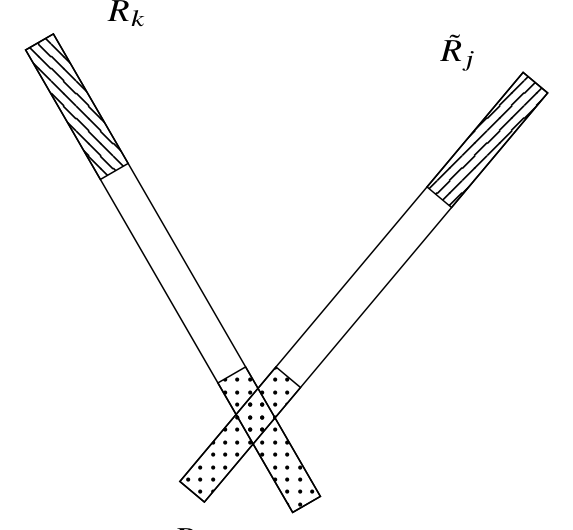
\includegraphics[width=0.36\textwidth]{figs/fig-5-1.png}
\caption{矩形与膨胀后的矩形.}
\label{fig:5.1}
\end{figure}

这在对足够大的 $N$ 时显然为假. 这意味着 $S_1$ 在 $L^p(\R^n)$（$n \geq 2$）上有界当且仅当 $p = 2$.

\section{Bochner--Riesz 算子: 球面求和}

Bochner--Riesz 算子，对 $\lambda > 0$ 定义为
\begin{align*}
  \widehat{T^{\lambda}f}(\xi)=(1-|\xi|^{2})_{+}^{\lambda}\widehat{f}(\xi),
\end{align*}
是球乘子的更光滑版本. 它们的核也可以用贝塞尔函数显式地求值:
\begin{align*}
  K_{\lambda}(x)=\pi^{-\lambda}\Gamma(1+\lambda)\left|x\right|^{-n/2-\lambda}J_{n/2+\lambda}(2\pi|x|),
\end{align*}
尽管这一事实对随后关于它们 $L^{p}$-有界性的讨论无关紧要.

若 $\lambda > (n-1)/2$（临界指数），则 $K_\lambda$ 可积，$T^\lambda$ 在每个 $L^p(\R^n)$（$1 \leq p \leq \infty$）上有界.

但当 $0 < \lambda < (n-1)/2$ 时，$K_\lambda$ 的衰减与奇异积分的 Calderón--Zygmund 理论相去甚远；事实上，一个明显的反例（$\widehat{f}$ 有界支集且 $|\xi| \leq 1$ 时 $\widehat{f}(\xi) \equiv 1$）表明 $T^\lambda$ 在区间
\begin{align*}
  \frac{2n}{n+1+2\lambda}<p<\frac{2n}{n-1-2\lambda}
\end{align*}
之外不可能有界.

但在这个区间内部，估计对径向函数 $f(|x|)$ 成立，对形如 $f(|x|)P_k(x)$ 的乘积也成立，其中 $P_k$ 是 $k$ 次球调和函数.

基于这些证据，人们提出了下面的猜想:

\begin{conjecture}\label{conj:5.5}
算子 $T^\lambda$ 在 $L^p(\R^n)$ 上有界，只要
\begin{align*}
  \frac{2n}{n+1+2\lambda}<p<\frac{2n}{n-1-2\lambda},\qquad 0<\lambda<\frac{n-1}{2}.
\end{align*}
\end{conjecture}

除 $n = 1$ 的情形外，该猜想只在二维被证明，本节的主要目的正是呈现其证明所涉及的思想.

\begin{theorem}\label{thm:5.6}
对 $0 < \lambda < 1/2$，算子 $T^\lambda$ 在
\begin{align*}
  \frac{4}{3+2\lambda}<p<\frac{4}{1-2\lambda}
\end{align*}
时于 $L^p(\R^2)$ 上有界.
\end{theorem}

乘子 $m_\lambda(\xi) = (1 - |\xi|^2)_{+}^\lambda$ 相当复杂，理解其性质的一个好策略是找出藏在 $m_\lambda$ 内部的 Calderón--Zygmund 理论的基本构件.

由于 $m_{\lambda}$ 是径向的，且在薄环上基本为常数，引入下列分解似乎合理:
\begin{align*}
  m_{\lambda}(\xi)=\sum_{k=0}^{\infty}(1-|\xi|^{2})_{+}^{\lambda}\phi_{k}(|\xi|),
\end{align*}
其中每个 $\phi_k$（$k \geq 1$）是支于区间 $[1-2^{-k}, 1-2^{-k+1}]$ 的光滑函数，满足 $|D^\alpha \phi_k| \leq C_\alpha 2^{k\alpha}$，$C_\alpha$ 与 $k$ 无关；且在区间 $1/2 \leq x \leq 1$ 上 $\sum_{k=1}^{\infty} \phi_k(x) \equiv 1$. 定义 $\phi_0 = 1 - \sum_{k=1}^{\infty} \phi_k$.

注意
\begin{align*}
  \phi_{j}(|\xi|)(1-|\xi|^{2})_{+}^{\lambda}\simeq 2^{-j\lambda}\phi_{j}(|\xi|),
\end{align*}
所以我们的问题化归为: 对 $j \to \infty$，得到乘子 $\phi_j(|\xi|)$ 范数增长的好的估计. 更精确地说，若我们能证明算子
\begin{align*}
  \widehat{T_{k}f}(\xi)=\phi_{k}(|\xi|)\widehat{f}(\xi)
\end{align*}
满足估计
\begin{align*}
  \left\|T_{k}f\right\|_{4}\lesssim k^{1/4}\left\|f\right\|_{4},\qquad f\in\mathcal{S}(\R^{2}),
\end{align*}
则定理 5.6 的证明将容易得到. 这是因为与估计 $\|T^k f\|_\infty \lesssim 2^{k/2}\|f\|_\infty$ 插值给出
\begin{align*}
  \left\|T_{k}f\right\|_{p}\lesssim k^{t/4}2^{k(1-t)/2}\left\|f\right\|_{p}.
\end{align*}
当 $1/p = t/4$ 且 $2 \leq p < 4/(1 - 2\lambda)$ 时，$1 - t < 2\lambda$，级数 $\sum_{j=1}^{\infty}2^{-j\lambda}j^{1/4}2^{j(1-t)/2}$ 收敛.

\begin{remark}\label{rem:5.7}
只要 $1 - t < 2\lambda$，上面的级数把幂 $j^{1/4}$ 换成 $j^\alpha$ 仍然收敛. 即，$T_k$ 在 $L^4(\R^2)$ 范数估计中的任何幂 $k^\alpha$ 都足以推出定理 5.6 的有效性，这为把定理推广到更一般的语境留出了灵活性.
\end{remark}

定理 5.6 将不过是下面命题的推论:

\begin{proposition}\label{prop:5.8}
设
\begin{align*}
  \widehat{S_{\delta}f}(\xi)=\phi(\delta^{-1}(1-|\xi|))\widehat{f}(\xi),
\end{align*}
其中 $0 < \delta < 1/2$，$\phi$ 是支于区间 $(-1,1)$ 的光滑函数. 存在与 $\delta$ 无关的有限常数 $C$，使
\begin{align*}
  \|S_{\delta}f\|_{4}\leq C\,|\log\delta|^{1/4}\|f\|_{4}
\end{align*}
对每个 Schwartz 类 $\mathcal{S}(\R^{2})$ 中的 $f$ 成立.
\end{proposition}

\begin{proof}
不失一般性，可以假设 $S_\delta$ 作用于其傅里叶变换 $\widehat{f}$ 支于角区域 $\{0 \leq \arg(\xi) \leq \pi/3\}$ 的函数 $f$ 上.

在单位圆上考虑光滑单位分解 $\psi_j$，$j = 1, 2, \ldots, [\delta^{-1/2}]$，使
\begin{align*}
  \psi_{j}(\theta)=\psi\bigl(\delta^{-1/2}\left(\theta-2\pi j\delta^{1/2}\right)\bigr),
\end{align*}
其中 $\psi$ 是支于单位区间的光滑函数（不失一般性，可设 $\delta^{-1/2}$ 是整数）.

有
\begin{align*}
  \widehat{S_{\delta}f}(|\xi|e^{i\theta})
  =\sum_{j=1}^{\delta^{-1/2}}\phi(\delta^{-1}(1-|\xi|))\psi_{j}(\theta)\widehat{f}(\xi)
  =\sum_{j}m_{j}(\xi)\widehat{f}(\xi)
  =\sum_{j}\widehat{T_{j}f}(\xi),
\end{align*}
\begin{align*}
  \int\Big|\sum_{j} T_{j} f\Big|^{4}\mathrm{d}x
  &=\int\Big|\sum_{j,k}T_{j} f(x)\,T_{k} f(x)\Big|^{2}\mathrm{d}x
  =\int\Big|\sum_{j,k}\widehat{T_{j} f}*\widehat{T_{k} f}(\xi)\Big|^{2}\mathrm{d}\xi\\
  &\lesssim\sum_{j,k}\int|\widehat{T_{j} f}*\widehat{T_{k} f}(\xi)|^{2}\mathrm{d}\xi
  =\int\Big(\sum_{j}|T_{j} f(x)|^{2}\Big)^{2}\mathrm{d}x,
\end{align*}
其中上述不等式中的关键点是: 集合族 $\supp(\widehat{T_j f}) + \supp(\widehat{T_k f})$ 具有与 $\delta$ 无关的有限重叠.

接下来，利用逐点估计
\begin{align*}
  \Big(\sum_{j}|T_{j}f(x)|^{2}\Big)^{1/2}
  \leq\Big(\sum_{j}|T_{2j}f(x)|^{2}\Big)^{1/2}
  +\Big(\sum_{j}|T_{2j+1}f(x)|^{2}\Big)^{1/2},
\end{align*}
并注意到右端两项具有相同的范数.

关于第一项，$m_{2j}(\xi)$ 的支集基本垂直于水平轴，我们可以找到一列沿竖直方向均匀分布的水平带 $E_j$，使
\begin{align*}
  \supp(m_{2j})\subset E_{2j}.
\end{align*}

\begin{figure}[htbp]
\centering
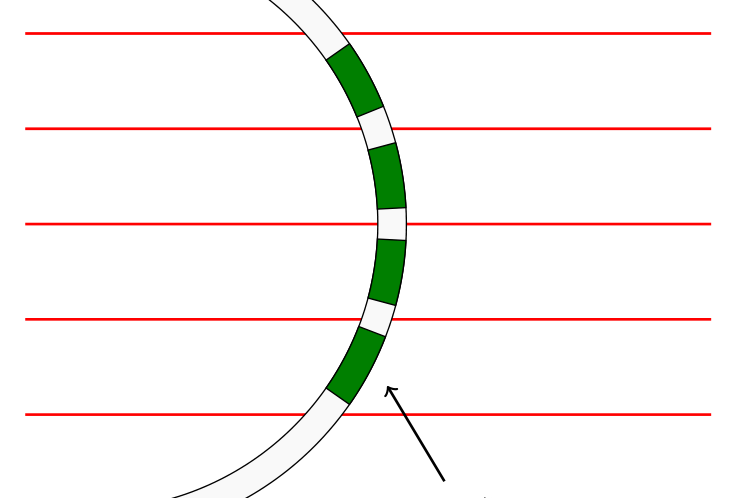
\includegraphics[width=0.44\textwidth]{figs/fig-5-2.png}
\caption{$G$-函数.}
\label{fig:5.2}
\end{figure}

于是 $m_{2j}(\xi) = m_{2j}(\xi)E_{2j}(\xi)$. 定义
\begin{align*}
  \widehat{P_{2j}f}(\xi)=E_{2j}(\xi)\widehat{f}(\xi),
\end{align*}
有
\begin{align*}
  \Big(\sum_{j}|T_{2j}f(x)|^{2}\Big)^{1/2}
  =\Big(\sum_{j}|T_{2j}P_{2j}f(x)|^{2}\Big)^{1/2}.
\end{align*}

一个初等的分部积分论证给出 $T_0$ 的核 $K_0$ 满足: 对每对整数 $\alpha, \beta \geq 0$，存在与 $\delta$ 无关的有限常数 $C_{\alpha,\beta}$，使
\begin{align*}
  |K_{0}(x,y)|\leq C_{\alpha,\beta}\delta^{3/2}|\delta x|^{-\alpha}|\delta^{1/2}y|^{-\beta},
\end{align*}
其中 $(x, y)$ 是 $\R^2$ 中的标准直角坐标.

于是算子 $T_{0}$ 逐点地被核为
\begin{align*}
  C\sum_{n=0}^{\infty}2^{-n}\frac{1}{\mu(R_{n}^{0})}\chi_{R_{n}^{0}}(x,y)
\end{align*}
的正算子控制，其中
\begin{align*}
  R_{n}^{0}=\{(x,y):|x|\leq 2^{n}\delta^{-1},\ |y|\leq 2^{n}\delta^{-1/2}\},
\end{align*}
$C$ 是与 $\delta$ 无关的适当常数. 用适当的旋转，对每一块 $T_{j}$ 得到类似的控制.

由于衰减 $2^{-n}$，只须证明: 对每个 $n$，函数
\begin{align*}
  \Big(\sum_{j}\Big|\frac{1}{\mu(R_{n}^{2j})}\chi_{R_{n}^{2j}}*P_{2j}f(x)\Big|^{2}\Big)^{1/2}
\end{align*}
的 $L^{4}$-范数以 $C|\log\delta|^{1/4}\|f\|_{4}$ 为界.

为看出这一点，取 $L^2(\R^2)$ 中的 $\omega \geq 0$，考虑积分
\begin{align*}
  \sum_{j}\int\Big|\frac{1}{\mu(R_{n}^{2j})}\chi_{R_{n}^{2j}}*P_{2j}f(x)\Big|^{2}\omega(x)\,\mathrm{d}x
  &\lesssim\sum_{j}\int|P_{2j}f(y)|^{2}\frac{1}{\mu(R_{n}^{2j})}\chi_{R_{n}^{2j}}*\omega(y)\,\mathrm{d}y\\
  &\lesssim\sum_{j}\int|P_{2j}f(y)|^{2}M\omega(y)\,\mathrm{d}y\\
  &\qquad\leq\Big\|\Big(\sum_{j}|P_{2j}f|^{2}\Big)^{1/2}\Big\|_{4}^{2}\|M\omega\|_{2},
\end{align*}
其中 $M$ 是第 3 章中对应离心率 $N = \delta^{-1/2}$ 矩形的 Kakeya 极大函数. 于是
\begin{align*}
  \Big\|\Big(\sum_{j}|T_{2j}f|^{2}\Big)^{1/2}\Big\|_{4}^{2}
  &\leq\sup_{\|\omega\|_{2}=1}\int\sum_{j}|T_{2j}f(x)|^{2}\omega(x)\,\mathrm{d}x\\
  &\lesssim|\log\delta|^{1/2}\Big\|\Big(\sum_{j}|P_{2j}f|^{2}\Big)^{1/2}\Big\|_{4}^{2},
\end{align*}
而命题将是下面引理的推论:
\end{proof}

\begin{lemma}\label{lem:5.9}
在 $\R^n$ 中，考虑格 $\mathcal{L} = \{Q_\nu\}_{\nu \in \Z^n}$. 即，平行多面体 $Q_\nu$ 全等、内部两两不交，且 $\R^n = \bigcup_\nu Q_\nu$.

对每个 $\nu \in \Z^n$ 定义算子
\begin{align*}
  \widehat{P_{\nu}f}(\xi)=Q_{\nu}(\xi)\widehat{f}(\xi)
\end{align*}
以及平方函数
\begin{align*}
  G f(x)=\Big(\sum_{\nu}|P_{\nu}f(x)|^{2}\Big)^{1/2}.
\end{align*}
则对每个 $s > 1$，存在有限常数 $C_s$，使对每个局部可积函数 $\omega \geq 0$ 与每个 $f \in \mathcal{S}(\R^n)$,
\begin{align*}
  \int_{\R^{n}}[G f(x)]^{2}\omega(x)\,\mathrm{d}x
  \leq C_{s}\int_{\R^{n}}|f(x)|^{2}A_{s}\omega(x)\,\mathrm{d}x,
\end{align*}
其中 $A_{s}\omega(x)=[M\omega^{s}(x)]^{1/s}$，$M$ 表示 $\R^{n}$ 中的强极大函数.
\end{lemma}

\begin{proof}
用方便的膨胀，不失一般性可设 $\mathcal{L}$ 是单位格，即 $Q_\nu$ 是以点 $\nu \in \Z^n$ 为中心的单位方体.

设 $\psi$ 是紧支集光滑函数，使 $\psi \equiv 1$ 于 $Q_0$ 内部. 对每个 $y \in Q_0$，考虑由
\begin{align*}
  m_{y}(z)=\sum_{\nu}\exp(2\pi i\nu\cdot y)\,\psi(z-\nu)
\end{align*}
给出的傅里叶乘子. 核 $\mu_y = \widehat{m}_y$ 是总变差有限的测度，对 $y \in Q_0$ 一致. 更精确地,
\begin{align*}
  \mu_{y}=\sum_{\nu}\widehat{\psi}(y+\nu)\,\delta_{y+\nu},
\end{align*}
其中 $\delta_{x}$ 表示 Dirac $\delta$ 函数. 于是
\begin{align*}
  |\mu_{y}*f(x)|^{2}\lesssim\sum_{\nu}(1+|\nu|)^{2n}\left|\widehat{\psi}(y+\nu)\right|^{2}|f(x-y-\nu)|^{2},
\end{align*}
利用 $\psi$ 速降的事实，对足够大的 $N$ 有
\begin{align*}
  \int_{\R^{n}}|\mu_{y}*f(x)|^{2}\omega(x)\,\mathrm{d}x
  \leq C_{N}\sum_{\nu}(1+|\nu|)^{2n-N}\int_{\R^{n}}|f(x)|^{2}\omega(x+y+\nu)\,\mathrm{d}x.
\end{align*}
选取 $N \geq 4n$，得
\begin{align*}
  \int_{Q_{0}}\int_{\R^{n}}&|\mu_{y}*f(x)|^{2}\omega(x)\,\mathrm{d}x\,\mathrm{d}y\\
  &\leq C_{N}\sum_{\nu}(1+|\nu|)^{2n-N}\int_{\R^{n}}|f(x)|^{2}\Big(\int_{Q_{0}}\omega(x+y+\nu)\,\mathrm{d}y\Big)\mathrm{d}x\\
  &\lesssim\int_{\R^{n}}|f(x)|^{2}M\omega(x)\,\mathrm{d}x,
\end{align*}
其中 $M$ 是 Hardy--Littlewood 极大函数.

但另一方面，若 $\widehat{T_{\nu}f}(\xi)=\psi(\xi-\nu)\widehat{f}(\xi)$，则有
\begin{align*}
  \mu_{y}*f(x)=\sum_{\nu}\exp(2\pi i\nu\cdot y)\,T_{\nu}f(x),
\end{align*}
以及
\begin{align*}
  \int_{Q_{0}}\int_{\R^{n}}\left|\mu_{y}*f(x)\right|^{2}\omega(x)\,\mathrm{d}x\,\mathrm{d}y
  =\sum_{\nu}\int_{\R^{n}}\left|T_{\nu}f(x)\right|^{2}\omega(x)\,\mathrm{d}x,
\end{align*}
由此得到所求的估计:
\begin{align*}
  \sum_{\nu}\int_{\R^{n}}&|P_{\nu}f(x)|^{2}\omega(x)\,\mathrm{d}x
  =\sum_{\nu}\int_{\R^{n}}|P_{\nu}T_{\nu}f(x)|^{2}\omega(x)\,\mathrm{d}x\\
  &\lesssim C_{s}\sum_{\nu}\int_{\R^{n}}|T_{\nu}f(x)|^{2}A_{s}\omega(x)\,\mathrm{d}x
  \lesssim C_{s}\int_{\R^{n}}|f(x)|^{2}A_{s}\omega(x)\,\mathrm{d}x.
\end{align*}
\end{proof}

\begin{remark}\label{rem:5.10}
引理~\ref{lem:5.9} 有一个更强的（无权重）版本，其中格被换成更一般的、各边平行于坐标轴的两两不交平行多面体族. 一维情形的证明由 J.~L.~Rubio de Francia \cite{b123} 获得，任意维数由 J.-L.~Journé \cite{b119} 获得.
\end{remark}

\section{向量值不等式}

现在考虑 Bochner--Riesz 算子的膨胀 $T_{R}^{\lambda}$:
\begin{align*}
  \widehat{T_{R}^{\lambda}f}(\xi)=(1-|\xi|^{2}/R^{2})_{+}^{\lambda}\widehat{f}(\xi),
\end{align*}
并设 $\{R_j\}$ 是正数的任何序列. 则有定理 5.6 的向量值版本.

\begin{theorem}\label{thm:5.11}
在 $\R^2$ 中，给定 $\lambda > 0$ 与 $4/(3+2\lambda) < p < 4/(1-2\lambda)$，存在有限常数 $C_{p,\lambda}$，使
\begin{align*}
  \left\|\Big(\sum_{j}|T_{R_{j}}^{\lambda}f_{j}|^{2}\Big)^{1/2}\right\|_{p}
  \leq C_{p,\lambda}\left\|\Big(\sum_{j}|f_{j}|^{2}\Big)^{1/2}\right\|_{p}.
\end{align*}
\end{theorem}

\begin{proof}
如定理 5.6 的证明，可以把估计化归为乘子支于薄环上的情形. 假设 $\phi: \R \to \R$ 是支于 $[-1,+1]$ 的光滑函数，定义
\begin{align*}
  \widehat{S_{j}^{\delta}f}(\xi)&=\phi(\delta^{-1}(1-|\xi|/R_{j}))\widehat{f}(\xi),\\
  \widehat{T_{j}^{n}f}(\xi)&=\psi_{n}(\arg(\xi))\widehat{S_{j}^{\delta}f}(\xi)=m_{j,n}(\xi)\widehat{f}(\xi),
\end{align*}
其中 $\{\psi_{n}\}$ 是命题 5.8 中引入的光滑角向单位分解.

不失一般性，还可以假设
\begin{align*}
  \supp(\widehat{f_{j}})\subset\{0\leq\arg(\xi)\leq\pi/3\},\qquad \text{对每个 } j.
\end{align*}
回忆 $\psi_n$ 支于 $|\theta-2\pi n/N| \leq 2\pi/N$，其中 $N = \delta^{-1/2}$（不失一般性可视为整数）. 这意味着 $m_{j,n}(\xi)$ 支于尺寸为 $R_j \delta \times R_j \delta^{1/2}$、方向为 $2\pi n/N$ 的``矩形''上.

证明分三步:

(a) 与定理 5.6 所用类似的论证允许把证明化归为不等式
\begin{align*}
  \left\|\Big(\sum_{j}|S_{j}^{\delta}f_{j}|^{2}\Big)^{1/2}\right\|_{4}
  \leq C|\log\delta|^{\alpha}\left\|\Big(\sum_{j}|f_{j}|^{2}\Big)^{1/2}\right\|_{4}.
\end{align*}

(b) 借助乘子的适当分解与若干几何论证，我们证明
\begin{align*}
  \left\|\Big(\sum_{j}|S_{j}^{\delta}f_{j}|^{2}\Big)^{1/2}\right\|_{4}
  \leq C|\log\delta|\left\|\Big(\sum_{j,n}|T_{j}^{n}f_{j}|^{2}\Big)^{1/2}\right\|_{4}.
\end{align*}

(c) 对 $T_j^n$ 的核的估计，连同引理 5.9 与定理 3.7，给出
\begin{align*}
  \left\|\Big(\sum_{j,n}|T_{j}^{n} f_{j}|^{2}\Big)^{1/2}\right\|_{4}
  \leq C|\log\delta|^{\beta}\left\|\Big(\sum_{j}|f_{j}|^{2}\Big)^{1/2}\right\|_{4}.
\end{align*}

第 (a) 部分留给读者.

关于第 (b) 部分，首先在每个 $|\log_2 \delta|$ 个相邻区间中只选出一个二进区间 $2^k < R \leq 2^{k+1}$，并且只允许 (b) 左端那些 $R_j$ 落在所选区间中的指标 $j$ 出现. 同时，对每四个相邻指标 $n$ 只取一个 $T_j^n$，并且只取那些支于角扇形 $\{0 \leq \arg(\xi) \leq \pi/3\}$ 者. 所有这些操作都会给不等式 (b) 贡献因子 $C|\log \delta|$.

(b) 的左端小于下面量的四次根的二倍:
\begin{align*}
  \sum_{R_{j}\leq R_{k}}\int\left|\Big(\sum_{n}T_{j}^{n} f_{j}\Big)\Big(\sum_{m}T_{k}^{m} f_{k}\Big)\right|^{2}.
\end{align*}
可以区分两类点对 $(j, k)$: 或 $R_j \leq R_k \leq 2R_j$，或 $R_j \leq \delta R_k$. 记上述和的两部分为 $\sum_{\mathrm{I}}$ 与 $\sum_{\mathrm{II}}$. 有
\begin{align*}
  \sum_{\mathrm{I}}
  =\sum_{\mathrm{I}}\int\left|\sum_{n,m}(\widehat{T_{j}^{n}f_{j}})\ast(\widehat{T_{k}^{m}f_{k}})\right|^{2}
  \leq 4\sum_{\mathrm{I}}\int\left|\sum_{n\leq m}\widehat{T_{j}^{n}f_{j}}\ast\widehat{T_{k}^{m}f_{k}}\right|^{2},
\end{align*}
一个简单的几何论证表明，对固定的 $j$ 与 $k$，对不同对 $n \leq m$，$\widehat{T_{j}^{n} f_{j}} * \widehat{T_{k}^{m} f_{k}}$ 的支集互不相交. 因此,
\begin{align*}
  \sum_{\mathrm{I}}\leq 4\int\sum_{\mathrm{I}}\sum_{n\leq m}|\widehat{T_{j}^{n}f_{j}}*\widehat{T_{k}^{m}f_{k}}|^{2}\leq 4A,
\end{align*}
其中
\begin{align*}
  A=\Big\|\Big(\sum_{j,n}|T_{j}^{n} f_{j}|^{2}\Big)^{1/2}\Big\|_{4}^{4}.
\end{align*}
其次注意，当 $(j,k)$ 属于情形 $\Sigma_{\mathrm{II}}$ 时，$R_{j} \leq \delta R_{k}$，且卷积
\begin{align*}
  \widehat{T_{j}^{n_{1}}f_{j}}*\widehat{T_{k}^{m_{1}}f_{k}},\qquad
  \widehat{T_{j}^{n_{2}}f_{j}}*\widehat{T_{k}^{m_{2}}f_{k}}
\end{align*}
的支集在 $m_1 \neq m_2$ 时不交. 则
\begin{align*}
  \sum_{\mathrm{II}}
  &=\sum_{\mathrm{II}}\int\Big|\sum_{m}\Big(\sum_{n}T_{j}^{n}f_{j}\Big)T_{k}^{m}f_{k}\Big|^{2}\\
  &\leq\Big[\int\Big(\sum_{j}\Big|\sum_{n}T_{j}^{n}f_{j}\Big|^{2}\Big)^{1/2}\Big]^{1/2}
   \cdot\Big[\int\Big(\sum_{k,m}|T_{k}^{m}f_{k}|^{2}\Big)^{2}\Big]^{1/2}
  \leq\sqrt{2}\left[\sum_{\mathrm{I}}+\sum_{\mathrm{II}}\right]^{1/2}A^{1/2},
\end{align*}
这就推出 (b).

为证明第 (c) 部分，首先注意对每个固定的 $j$，可以选取如引理 5.9 那样的矩形网格，使每个乘子 $m_{j,n}(\xi)$ 支于网格中的某个矩形 $Q_{j}^{n}$ 内.

若 $\widehat{P_j^n f} = Q_j^n\cdot\widehat{f}$ 是相应的傅里叶乘子，则有恒等式
\begin{align*}
  T_{j}f_{j}=T_{j}^{n}P_{j}^{n}f_{j}.
\end{align*}
此外，分部积分论证（如定理 5.6 中）表明 $T_j^n$ 的核被
\begin{align*}
  C\sum_{\nu=0}^{\infty}2^{-\nu}\frac{1}{|R_{\nu,j}^{n}|}R_{\nu,j}^{n}(x)
\end{align*}
控制，其中 $R_{\nu,j}^n$ 是尺寸 $2^\nu\delta^{-1} \times 2^\nu\delta^{-1/2}$、方向角 $2\pi\delta^{1/2}n$ 的矩形，$C$ 与 $n$、$j$ 和 $\delta > 0$ 无关.

于是，为估计 $A$，需要对 $\nu$ 一致地估计
\begin{align*}
  \Big[\sum_{j,n}\Big(\frac{1}{|R_{\nu,j}^{n}|}R_{\nu,j}^{n}*|P_{j}^{n}f_{j}|\Big)^{2}\Big]^{1/2}
\end{align*}
的 $L^{4}$-范数. 若 $w \geq 0$ 属于 $L^2(\R^2)$，有
\begin{align*}
  &\sum_{j,n}\int\left[\frac{1}{\left|R^{n}_{\nu,j}\right|}R^{n}_{\nu,j}*|P^{n}_{j} f_{j}|\right]^{2}\omega(x)\,\mathrm{d}x
  \leq\sum_{j,n}\int|P^{n}_{j} f_{j}(y)|^{2}\left[\frac{1}{\left|R^{n}_{\nu,j}\right|}R^{n}_{\nu,j}*\omega(y)\right]\mathrm{d}y\\
  &\quad\leq\sum_{j,n}\int|P^{n}_{j} f_{j}(y)|^{2}M\omega(y)\,\mathrm{d}y
  \leq C_{s}\sum_{j}\int|f_{j}(y)|^{2}A_{s}(M\omega)(y)\,\mathrm{d}y\\
  &\quad\leq\widetilde{C}_{s}\left\|\Big(\sum_{j}|f_{j}|^{2}\Big)^{1/2}\right\|_{4}^{2}\|M\omega\|_{2}
  \leq C\left|\log\delta\right|^{1/2}\|\omega\|_{2}\left\|\Big(\sum_{j}|f_{j}|^{2}\Big)^{1/2}\right\|_{4}^{2},
\end{align*}
其中再次用到了引理 5.9 与第 3 章 Kakeya 极大函数的估计.
\end{proof}

\section{一个角平方函数}

在 $\R^2$ 中，考虑角 $\omega_j = 2\pi j/N$，$j = 0,1,\ldots,N-1$，区域
\begin{align*}
  \Delta_{j}=\{\xi:\omega_{j}\leq\arg(\xi)\leq\omega_{j+1}\},
\end{align*}
傅里叶乘子
\begin{align*}
  \widehat{S_{j}f}(\xi)=\Delta_{j}(\xi)\widehat{f}(\xi)
\end{align*}
以及相伴的平方函数
\begin{align*}
  G(f)(x)=\left(\sum_{j}\left|S_{j}f(x)\right|^{2}\right)^{1/2}.
\end{align*}

\begin{theorem}\label{thm:5.12}
存在与 $N$ 无关的常数 $a$ 与 $C$，使
\begin{align*}
  \left\|G(f)\right\|_{4}\leq C\left[\log N\right]^{a}\left\|f\right\|_{4}
\end{align*}
对每个 Schwartz 类 $\mathcal{S}(\R^{2})$ 中的 $f$ 成立.
\end{theorem}

设 $\{\psi_j\}$ 是如定理 5.11 中的角截断函数，使 $\psi_j \equiv 1$ 于 $\Delta_j$，$\supp(\psi_j) \subset \Delta_{j-1} \cup \Delta_j \cup \Delta_{j+1}$，写
\begin{align*}
  \widehat{\widetilde{S}_{j}f}(\xi)=\psi_{j}(\xi)\widehat{f}(\xi),\qquad
  \widetilde{G}f(x)=\Big(\sum_{j}|\widetilde{S}_{j}f(x)|^{2}\Big)^{1/2}.
\end{align*}
于是，借助第 3 章 Kakeya 极大函数的估计，定理 5.12 将是下面命题的推论.

\begin{proposition}\label{prop:5.13}
存在与 $N$ 无关的有限常数 $a$ 与 $C$，使:
\begin{align*}
  \|\widetilde{G}(f)\|_{4}\leq C\left[\log N\right]^{a}\|f\|_{4}.
\end{align*}
\end{proposition}

设 $\{\phi_n\}$ 是满足 $\supp(\phi_n) \subset (2^{n-1}, 2^{n+1})$ 与 $|D_x^\alpha \phi_n| \leq C_\alpha 2^{-n\alpha}$ 的光滑函数，定义
\begin{align*}
  \widehat{\widetilde{S}_{j,n}f}(\xi)=\phi_{n}(|\xi|)\psi_{j}(\xi)\widehat{f}(\xi),\qquad
  \widetilde{G}_{n}f(x)=\Big(\sum_{j}|\widetilde{S}_{j,n}f(x)|^{2}\Big)^{1/2}.
\end{align*}
于是，第一步我们将证明估计
\begin{align*}
  \|\widetilde{G}_{n}f\|_{4}\leq C\left[\log N\right]^{a}\|f\|_{4},
\end{align*}
常数 $C$ 与 $a$ 与 $n$ 和 $N$ 无关. 但一个简单的膨胀论证表明，只须证明 $n = 1$ 的情形.

第二步，我们将把这些估计合在一起得到命题的证明. 还要注意到，不失一般性，可以假设函数 $f$ 的傅里叶变换支于区域
\begin{align*}
  \{\xi:0\leq\arg(\xi)\leq\pi/4\}.
\end{align*}
我们必须计算
\begin{align*}
  \|\widetilde{G}_{1}f\|_{4}^{4}
  =\sum_{j,k}\int_{\R^{2}}\left|\widetilde{S}_{j}f(x)\widetilde{S}_{k}f(x)\right|^{2}\mathrm{d}x
  =\sum_{|j-k|\leq 4}(\cdots)+\sum_{|j-k|>4}(\cdots)=\mathrm{I}+\mathrm{II}.
\end{align*}
接着把 $\phi_1(|\xi|)\psi_j(\xi)$ 的支集进一步分解成 $N^{1/2}$ 个部分 $\Delta_j^\alpha$，$\alpha = 1, \ldots, N^{1/2}$，其中
\begin{align*}
  \Delta_{j}^{\alpha}=\left\{\xi\in\supp(\phi_{1}\cdot\psi_{j}):\alpha N^{-1/2}\leq|\xi|-1\leq(\alpha+1)N^{-1/2}\right\}
\end{align*}
（同样，不失一般性可设 $N^{1/2}$ 是整数）. 当 $|j - k| \geq 4$ 时，集合 $\Delta_j^\alpha + \Delta_k^\beta$ 的重叠有界，且对 $N$ 一致.

于是，再次用 Plancherel 定理，得
\begin{align*}
  \mathrm{II}
  &\leq\sum_{|j-k|\geq 4}\sum_{\alpha,\beta}\int_{\R^{2}}|\widetilde{S}_{j}^{\alpha}f(x)\;\widetilde{S}_{k}^{\beta}f(x)|^{2}\mathrm{d}x
  \leq\left\|\Big(\sum_{j,\alpha}|\widetilde{S}_{j}^{\alpha}f|^{2}\Big)^{1/2}\right\|_{4}^{4},
\end{align*}
其中
\begin{align*}
  \widehat{\widetilde{S}_{j}^{\alpha}f}(\xi)=\phi_{1}(|\xi|)\psi_{j}(\xi)\eta_{\alpha}(|\xi|)\widehat{f}(\xi),
\end{align*}
$\eta_\alpha$ 是适应的光滑截断族，即在 $\phi_1\psi_j$ 的支集上有 $\sum_\alpha \eta_\alpha(|\xi|) \equiv 1$，且
\begin{align*}
  \supp\eta_{\alpha}\subset(1+\alpha N^{-1/2},1+(\alpha+2)N^{-1/2}),\qquad
  |D_{x}^{m}\eta_{\alpha}|\leq C_{m}N^{m/2}.
\end{align*}
注意
\begin{align*}
  \mathrm{I}
  &\leq\int\left(\sum_{j}|\widetilde{S}_{j} f|^{4}\right)
  \leq\int\left(\sum_{j}|\widetilde{S}_{j} f|^{2}\right)\cdot\left(\sup_{j}|\widetilde{S}_{j} f(x)|^{2}\right)\mathrm{d}x\\
  &\leq\left(\int\sum_{j,k}|\widetilde{S}_{j} f(x)\widetilde{S}_{k} f(x)|^{2}\mathrm{d}x\right)^{1/2}\left[\int|M_{N} f(x)|^{4}\right]^{1/2}\\
  &\leq\frac{1}{2}\varepsilon\left(\mathrm{I}+\mathrm{II}\right)+\frac{1}{2}\frac{1}{\varepsilon}C\left(\log N\right)^{a}\|f\|_{4}^{4}
\end{align*}
对每个 $\varepsilon > 0$ 成立. 因此，适当地选取 $\varepsilon$，只须证明估计
\begin{align*}
  \mathrm{II}\lesssim[\log N]^{a}\left\|{f}\right\|_{4}^{4}.
\end{align*}
为此，设 $\omega \geq 0$ 满足 $\|\omega\|_2 = 1$，考虑积分
\begin{align*}
  \sum_{j,\alpha}\int|\widetilde{S}_{j}^{\alpha}f(x)|^{2}\omega(x)\,\mathrm{d}x
  &=\sum_{\alpha=1}^{N^{1/2}}\int\Big|\sum_{j}\widetilde{S}_{j}^{\alpha}f(x)\Big|^{2}\omega(x)\,\mathrm{d}x\\
  &=\sum_{\alpha=1}^{N^{1/2}}\sum_{\tau=0}^{N^{1/2}}\int\Big|\sum_{j=\tau N^{1/2}}^{(\tau+1)N^{1/2}}\widetilde{S}_{j}^{\alpha}f(x)\Big|^{2}\omega(x)\,\mathrm{d}x\\
  &=\sum_{\alpha=1}^{N^{1/2}}\sum_{\tau=0}^{N^{1/2}}\int\Big|\sum_{j=\tau N^{1/2}}^{(\tau+1)N^{1/2}}\widetilde{S}_{j}^{\alpha}E_{j}^{\alpha}f(x)\Big|^{2}\omega(x)\,\mathrm{d}x,
\end{align*}
其中 $E_j^\alpha$ 是两两不交的矩形，平行于 $\Delta_j$ 的角平分线，尺寸约为 $N^{-1/2} \times N^{-1}$，满足 $E_j^\alpha \supset \phi_1\psi_j\eta_\alpha$；算子 $E_j^\alpha$ 由公式
\begin{align*}
  \widehat{E_{j}^{\alpha}f}(\xi)=E_{j}^{\alpha}(\xi)\widehat{f}(\xi)
\end{align*}
定义，这里我们再次使用了以同一符号 $E_{j}^{\alpha}$ 表示集合、其示性函数以及相伴傅里叶乘子的约定.

我们现在可以应用引理 5.9:
\begin{align*}
  \sum_{j,\alpha}\int\left|\widetilde{S}_{j}^{\alpha}f(x)\right|^{2}\omega(x)\,\mathrm{d}x
  &=\sum_{j,\alpha}\int\left|\widetilde{S}_{j}^{\alpha}E_{j}^{\alpha}f(x)\right|^{2}\omega(x)\,\mathrm{d}x\\
  &\lesssim\sum_{\alpha=1}^{N^{1/2}}\sum_{\tau=0}^{N^{1/2}}\int|Q_{\alpha}^{\tau}f(x)|^{2}M_{N}\omega(x)\,\mathrm{d}x,
\end{align*}
因为如定理 5.11，$\widetilde{S}_{j}^{\alpha}$ 的核被一个和
\begin{align*}
  C\sum_{\nu=0}^{\infty}2^{-\nu}\frac{1}{|R_{j,n}^{\alpha}|}R_{j,n}^{\alpha}(x)
\end{align*}
控制，其中 $R_{j,n}^{\alpha}$ 是 $j$ 方向上离心率 $N^{1/2}$ 的矩形. 这里对每个 $\alpha, \tau = 1, \ldots, N^{1/2}$，$Q_{\alpha}^{\tau}$ 现在是边长 $\sim N^{-1/2}$ 的正方形，族 $\{Q_{\alpha}^{\tau}\}$ 有普适有界的重叠.

再应用一次引理 5.9，连同 Kakeya 极大函数的已知估计，即得所求不等式.

为结束证明，把``二进''截断函数 $\phi_n$ 的指标按 $\bmod[\log_2 N]$ 分成剩余类，把方向指标 $j$ 按 $\bmod(4)$ 分成类，并应用定理 5.11 的同样方法.

\section{极大 Bochner--Riesz 算子: 逐点收敛}

对 $\lambda > 0$，极大函数
\begin{align*}
  T_{*}^{\lambda}f(x)=\sup_{R>0}|T_{R}^{\lambda}f(x)|,
\end{align*}
其中 $T_{R}^{\lambda}f(\xi)=(1-|\xi|^{2}/R^{2})_{+}^{\lambda}\widehat{f}(\xi)$，控制着当 $R$ 趋于无穷时 $T_{R}^{\lambda}f(x)$ 到 $f(x)$ 的几乎处处收敛.

利用单位球在边界附近厚度 $\delta$ 的冠状环的标准分解（$\delta = 2^{-k}$，$k = 1, 2, \ldots$），$T_*$ 的 $L^p$-有界性化归为对
\begin{align*}
  S_{*}^{\delta}f(x)=\sup_{R>0}|S_{R}^{\delta}f(x)|
\end{align*}
得到好的估计，其中
\begin{align*}
  \widehat{S_{R}^{\delta}f}(\xi)=\phi(|\xi|,R)\widehat{f}(\xi),
\end{align*}
$\phi$ 是任何满足下列条件的光滑函数:
\begin{align*}
  \supp\phi(\cdot,t)\subset(t-t\delta,t+t\delta),\qquad
  |D_{r}^{\alpha}\phi(r,t)|\leq C_{\alpha}(t\delta)^{-\alpha},
\end{align*}
\begin{align*}
  D_{t}\phi(r,t)=\psi(r,t)(t\delta)^{-1},
\end{align*}
\begin{align*}
  \supp\psi(r,t)\subset(t-t\delta,t+t\delta),\qquad
  |D_{r}^{\alpha}\psi(r,t)|\leq C_{\alpha}(t\delta)^{-\alpha}.
\end{align*}
一个例子是
\begin{align*}
  \phi(|\xi|,t)=\varphi\left(\frac{|\xi|-t}{\delta t}\right),
\end{align*}
其中 $\varphi$ 是支于 $(-1,+1)$ 的光滑函数.

\begin{theorem}\label{thm:5.14}
$S_{*}^{\delta}$ 在 $L^2(\R^n)$ 上有界.
\end{theorem}

\begin{corollary}\label{cor:5.15}
当 $\lambda > 0$ 时，对每个 $f \in L^2(\R^n)$，$\lim_{R \to \infty} T_R^\lambda f(x) = f(x)$ 几乎处处成立.
\end{corollary}

\begin{proof}[定理~\ref{thm:5.14} 的证明]
有
\begin{align*}
  (S_{R}^{\delta}f(x))^{2}
  =\int_{0}^{R}\frac{\mathrm{d}}{\mathrm{d}t}(S_{t}^{\delta}f(x))^{2}\,\mathrm{d}t
  =2\int_{0}^{R}S_{t}^{\delta}f(x)\cdot\frac{\mathrm{d}}{\mathrm{d}t}(S_{t}^{\delta}f(x))\,\mathrm{d}t,
\end{align*}
由此得估计
\begin{align*}
  S_{*}^{\delta}f(x)
  &\leq\delta^{-1/2}\Big(\int_{0}^{\infty}\left|S_{t}^{\delta}f(x)\right|^{2}\frac{\mathrm{d}t}{t}\Big)^{1/2}
   +\delta^{1/2}\Big(\int_{0}^{\infty}\left|\frac{\mathrm{d}}{\mathrm{d}t}S_{t}^{\delta}f(x)\right|^{2}t\,\mathrm{d}t\Big)^{1/2}\\
  &=\delta^{-1/2}G_{1}^{\delta}f(x)+\delta^{1/2}G_{2}^{\delta}f(x),
\end{align*}
以及
\begin{align*}
  \int_{\R^{n}}|G_{1}^{\delta}f(x)|^{2}\,\mathrm{d}x
  =\int_{\R^{n}}\Big(\int_{0}^{\infty}|\phi(|\xi|,t)|^{2}\frac{\mathrm{d}t}{t}\Big)|\widehat{f}(\xi)|^{2}\,\mathrm{d}\xi
  \leq C\delta\|f\|_{2}^{2},
\end{align*}
\begin{align*}
  \int_{\R^{n}}|G_{2}^{\delta}f(x)|^{2}\,\mathrm{d}x
  =\int_{\R^{n}}\Big(\int_{0}^{\infty}|\psi(|\xi|,t)|^{2}\frac{\mathrm{d}t}{t}\Big)|\widehat{f}(\xi)|^{2}\,\mathrm{d}\xi
  \leq C\delta^{-1}\|f\|_{2}^{2}.
\end{align*}
\end{proof}

在维数 $n = 2$ 中，定理 5.14 容许若干改进.

首先考虑 $\{R_j\}$ 是缺项的，即对每个 $j$ 有 $R_{j+1}/R_j > \rho > 1$，并考虑相伴的极大算子
\begin{align*}
  M_{*}^{\lambda}f(x)=\sup_{j}|T_{R_{j}}^{\lambda}f(x)|.
\end{align*}
则有:

\begin{theorem}\label{thm:5.16}
对 $0 < \lambda < 1/2$，极大算子 $M_{*}^{\lambda}$ 在 $L^p(\R^2)$ 上有界，当且仅当 $4/(3+2\lambda) < p < 4/(1-2\lambda)$.
\end{theorem}

\begin{proof}
用定理 5.11 引入的记号与类似论证，只须证明估计
\begin{equation}\label{eq:5.3}
  \left\|\Big(\sum_{j}|S_{j}^{\delta}f|^{2}\Big)^{1/2}\right\|_{4}
  \leq C\left|\log\delta\right|^{a}\|f\|_{4}
\end{equation}
对某个与 $\delta > 0$ 无关的有限常数 $a$ 与 $C$ 成立，其中
\begin{align*}
  \widehat{S_{j}^{\delta}f}(\xi)=\phi(\delta^{-1}\left(1-|\xi|/R_{j}\right))\widehat{f}(\xi).
\end{align*}
注意，不失一般性，只须对傅里叶变换 $\widehat{f}$ 支于角 $\{\xi : 0 \leq \arg(\xi) \leq \pi/3\}$ 的函数 $f$ 证明 \eqref{eq:5.3}.

由于当 $1 < \rho \leq 2$ 时，每个二进区间 $[2^l, 2^{l+1}]$ 至多含 $1 + |\log \delta|$ 个缺项集 $\{R_j\}$ 的元素，我们也可以（再次不失一般性）假设 $\rho \geq 2$，从而每个二进区间至多含一个 $R_j$.

于是 \eqref{eq:5.3} 借助定理 5.11 证明中发展的不等式容易得出. 细节留给读者.
\end{proof}

\begin{theorem}\label{thm:5.17}
对 $0 < \lambda < 1/2$，极大算子
\begin{align*}
  T^{\lambda}_{*}f(x)=\sup_{R>0}|T^{\lambda}_{R}f(x)|
\end{align*}
在 $2 \leq p < 4/(1 - 2\lambda)$ 时于 $L^p(\R^2)$ 上有界.
\end{theorem}

考虑到估计
\begin{align*}
  \sup_{R>0}|S_{R}^{\delta}f(x)|\lesssim\delta^{-1/2}M f(x),
\end{align*}
其中 $M$ 表示 Hardy--Littlewood 极大函数，$S_{R}^{\delta}f$ 如前由
\begin{align*}
  \widehat{S_{R}^{\delta}f}(\xi)=\phi(|\xi|,R)\widehat{f}(\xi)
\end{align*}
给出，定理 5.17 的证明由下面结果中给出的平方函数
\begin{align*}
  G f(x)=\Big(\int_{0}^{\infty}|S_{t}^{\delta}f(x)|^{2}\frac{\mathrm{d}t}{t}\Big)^{1/2}
\end{align*}
的估计，经标准插值得到.

\begin{lemma}\label{lem:5.18}
存在有限常数 $a$ 与 $C$，使
\begin{align*}
  \left\|G f\right\|_{4}\leq C|\log\delta|^{a}\delta^{1/2}\left\|f\right\|_{4},\qquad f\in\mathcal{S}(\R^{2}).
\end{align*}
\end{lemma}

\begin{proof}
不失一般性，可设 $\supp(\widehat{f}) \subset \{\xi : 0 \leq \arg(\xi) \leq \pi/3\}$，且 $\delta^{-1/2} = N^{1/2}$ 是整数.

设 $\{\psi_j\}_{j=1}^N$ 是光滑单位分解，使 $\psi_j$ 是 $\psi_0$ 的旋转，且为 $0$ 次齐次. 此外，令 $\psi_j$ 在 $\Delta_{j-1} \cup \Delta_j \cup \Delta_{j+1}$ 之外为 $0$，其中 $\Delta_j$ 是角区域
\begin{align*}
  \{\xi:j\delta^{1/2}\leq\arg(\xi)\leq(j+1)\delta^{1/2}\}.
\end{align*}
即
\begin{align*}
  \sum_{j}\psi_{j}(e^{2\pi i\theta})\equiv 1,\qquad
  |D^{\alpha}_{\theta}\psi_{j}|\leq C_{\alpha}\delta^{-\alpha/2}
\end{align*}
对适当的、与 $\delta$ 无关的常数 $C_{\alpha}$ 成立.

再设 $\{\Theta_k\}$ 是区间 $[1, \infty)$ 上的光滑``二进''单位分解，满足 $\supp(\Theta_k) \subset (2^{k-1}, 2^{k+2})$ 且对每个 $k, \alpha$ 及适当的常数 $C_\alpha$ 有 $|D^\alpha\Theta_k| \leq C_\alpha 2^{-k\alpha}$.

此外，对每个 $j = 1, \ldots, N^{1/2}$ 与 $k$，引入光滑截断函数 $\varphi_{\sigma}^{j,k}$，$\sigma = 1, \ldots, N$，使
\begin{align*}
  \sum_{k}\sum_{\sigma}\varphi_{\sigma}^{j,k}(\xi)=1,\qquad \xi\in\supp(\psi_{j}),
\end{align*}
且 $\supp(\varphi_{\sigma}^{j,k}) \subset (R_{\sigma}^{j,k})^{*}$，其中 ($^{*}$) 表示矩形 $R_{\sigma}^{j,k}$ 的 4 倍膨胀；$R_{\sigma}^{j,k}$ 含于 $\Delta_j \cap \{2^{k-1} < |\xi| < 2^{k+2}\}$，尺寸为 $2^{k-1}\delta \times 2^{k-1}\delta^{1/2}$，两边分别沿 $\Delta_j$ 角平分线方向及其垂直方向（见下图 5.3）.

\begin{figure}[htbp]
\centering
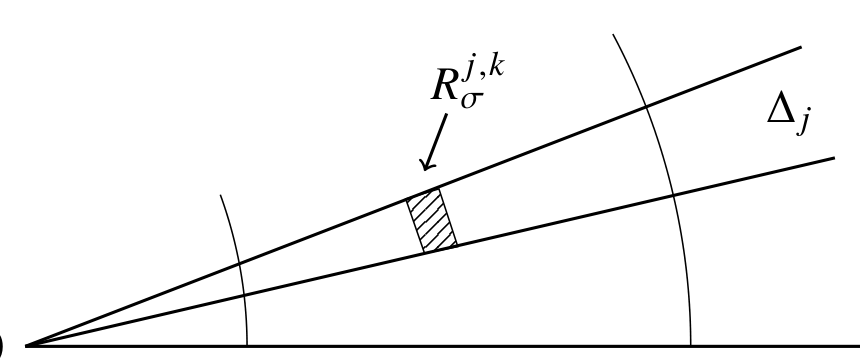
\includegraphics[width=0.5\textwidth]{figs/fig-5-3.png}
\caption{矩形 $R_{\sigma}^{j,k}$.}
\label{fig:5.3}
\end{figure}

此外，假设函数 $\varphi_{\sigma}^{j,k}$ 与 $R_{\sigma}^{j,k}$ 相适应；更精确地,
\begin{align*}
  |D_{v}^{\alpha}\varphi_{\sigma}^{j,k}|\leq
  \begin{cases}
    C_{\alpha}\left(\delta2^{k}\right)^{-\alpha}, & \text{若 } v \text{ 是角平分线方向},\\
    C_{\alpha}\left(\delta^{1/2}2^{k}\right)^{-\alpha}, & \text{若 } v \text{ 垂直于角平分线}.
  \end{cases}
\end{align*}
则
\begin{align*}
  \widehat{S_{t}^{\delta}f}(\xi)=\sum_{k,j,\sigma}\widehat{Q_{k,j,\sigma}^{t}f}(\xi),
\end{align*}
其中
\begin{align*}
  \widehat{Q_{k,j,\sigma}^{t}f}(\xi)=\Theta_{k}(\xi)\phi(|\xi|,t)\psi_{j}(\xi)\varphi_{\sigma}^{j,k}(\xi)\widehat{f}(\xi).
\end{align*}
接着，简化支集的几何: 把 $k$-指标按 $\bmod[|\log_{2}(\delta)|]$ 分成剩余类，使得同一剩余类 $I$ 中、对应不同值 $k_1 > k_2$ 的两个矩形 $R_{\sigma_1}^{j_1,k_1}$ 与 $R_{\sigma_2}^{j_2,k_2}$ 满足: $R_{\sigma_1}^{j_1,k_1}$ 的较小尺寸大于 $2^{k_2}$，即 $2^{k_1}\delta > 2^{k_2}$.

我们还可以假设其他指标 $j$ 与 $\sigma$ 分别取自剩余类 $J$ 与 $\Sigma$（$\bmod 8$）.

于是，除一个允许的因子 $|\log \delta|$ 外，引理将来自估计
\begin{align*}
  \left\|G_{I,J,\Sigma}(f)\right\|_{4}\lesssim\left|\log\delta\right|^{a}\left\|f\right\|_{4}
\end{align*}
对剩余类 $I$，$J$ 与 $\Sigma$ 的任何取法成立，其中
\begin{align*}
  G_{I,J,\Sigma}(f)(x)=\Big(\int_{0}^{\infty}\Big|\sum_{k\in I}\sum_{j\in J}\sum_{\sigma\in\Sigma}Q_{k,j,\sigma}^{t}f(x)\Big|^{2}\frac{\mathrm{d}t}{t}\Big)^{1/2}.
\end{align*}
为简化记号，下面将略去符号 $I, J, \Sigma$，并假设求和指标属于那些固定的剩余类.

有
\begin{align*}
  \left\|G(f)\right\|_{4}^{4}
  =\int_{0}^{\infty}\int_{0}^{\infty}\frac{\mathrm{d}t}{t}\frac{\mathrm{d}u}{u}
  \Big(\int_{\R^{2}}\Big|\sum_{k_{1},j_{1},\sigma_{1}}Q_{k_{1},j_{1},\sigma_{1}}^{t}f(x)
  \sum_{k_{2},j_{2},\sigma_{2}}Q_{k_{2},j_{2},\sigma_{2}}^{u}f(x)\Big|^{2}\mathrm{d}x\Big),
\end{align*}
对内部积分应用 Plancherel 定理，得
\begin{align*}
  \left\|G(f)\right\|_{4}^{4}
  =\int_{0}^{\infty}\int_{0}^{\infty}\frac{\mathrm{d}t}{t}\frac{\mathrm{d}u}{u}
  \Big(\int_{\R^{2}}\Big|\sum_{k_{1},j_{1},\sigma_{1}}\sum_{k_{2},j_{2},\sigma_{2}}
  \Omega_{k_{1},j_{1},\sigma_{1}}^{k_{2},j_{2},\sigma_{2}}(\xi)\Big|^{2}\mathrm{d}\xi\Big),
\end{align*}
其中 $\Omega_{k_{1},j_{1},\sigma_{1}}^{k_{2},j_{2},\sigma_{2}}$ 是
\begin{align*}
  \Theta_{k_{1}}(\xi)\phi(|\xi|,t)\psi_{j_{1}}(\xi)\varphi_{\sigma_{1}}^{j_{1},k_{1}}(\xi)
  \quad\text{与}\quad
  \Theta_{k_{2}}(\xi)\phi(|\xi|,u)\psi_{j_{2}}(\xi)\varphi_{\sigma_{2}}^{j_{2},k_{2}}(\xi)
\end{align*}
的卷积.

现在考虑对 $\Theta_k$，$\psi_j$ 与 $\varphi_\sigma^{j,k}$ 支集所加的条件，得
\begin{align*}
  \|G(f)\|_{4}^{4}\lesssim\int_{\R^{2}}
  \Big(\int_{0}^{\infty}\sum_{k,j,\sigma}\left|Q_{k,j,\sigma}^{t}f(x)\right|^{2}\frac{\mathrm{d}t}{t}\Big)^{2}\mathrm{d}x,
\end{align*}
即只须估计
\begin{align*}
  \Big[\int_{0}^{\infty}\sum_{k,j,\sigma}|Q_{k,j,\sigma}^{t} f(x)|^{2}\frac{\mathrm{d}t}{t}\Big]^{1/2}
\end{align*}
的 $L^{4}$-范数. 为此，首先注意对每组指标 $(k, j, \sigma)$ 与任何函数 $g \in \mathcal{S}(\R^2)$，有逐点不等式
\begin{align*}
  \int_{0}^{\infty}|Q_{k,j,\sigma}^{t}(g)(x)|^{2}\frac{\mathrm{d}t}{t}
  \lesssim\delta\sup_{t}|Q_{k,j,\sigma}^{t}(g)(x)|^{2}.
\end{align*}
这是因为
\begin{align*}
  \{t:Q^{t}_{k,j,\sigma}g(x)\neq 0\}
  &\subset\big\{t:\supp(\widehat{Q^{t}_{k,j,\sigma}g})\ \text{非空}\big\}\\
  &\subset\big\{t:\exists\xi,\ \Theta_{k}(\xi)\phi(|\xi|,t)\varphi^{j,k}_{\sigma}(\xi)\psi_{j}(\xi)\neq 0\big\}=E_{k,j,\sigma},
\end{align*}
而由 $\Theta_{k}$，$\phi$，$\psi_{j}$ 与 $\varphi_{\sigma}^{j,k}$ 的定义，容易得出
\begin{align*}
  \int_{0}^{\infty}E_{k,j,\sigma}(t)\frac{\mathrm{d}t}{t}\lesssim\delta.
\end{align*}
分部积分论证给出核（即 $\Theta_k \phi(|\xi|,t)\varphi_\sigma^{j,k}(\xi)\psi_j(\xi)$ 的傅里叶变换）在离心率 $\delta^{-1/2} = N^{1/2}$ 矩形平均方面的估计，由此得估计
\begin{align*}
  \sup_{t}|Q_{k,j,\sigma}^{t}g(x)|\lesssim M_{\delta^{-1/2}}(\widetilde{Q}_{k,j,\sigma}g)(x),
\end{align*}
其中 $M_{\delta^{-1/2}}$ 表示离心率 $\delta^{-1/2}$ 矩形的 Kakeya 极大函数,
\begin{align*}
  \widehat{\widetilde{Q}_{k,j,\sigma}g}(\xi)=\widetilde{\Theta}_{k}(\xi)\widetilde{\varphi}_{\sigma}^{j,k}(\xi)\widehat{f}(\xi),
\end{align*}
$\widetilde{\Theta}_{k}$ 与 $\widetilde{\varphi}_{\sigma}^{j,k}$ 是分别满足与 $\Theta_{k}$ 和 $\varphi_{\sigma}^{j,k}$ 相同估计、并在其支集上恒等于 $1$ 的适当截断.

于是对每个 $\omega \in L^2(\R^2)$，得
\begin{align*}
  \int_{0}^{\infty}&\int_{\R^{2}}|G f(x)|^{2}\omega(x)\,\mathrm{d}x\,\frac{\mathrm{d}t}{t}
  \lesssim\delta\sum_{j,k,\sigma}\int_{\R^{2}}|\widetilde{Q}_{j,k,\sigma}f(x)|^{2}M_{\delta^{-1/2}}\omega(x)\,\mathrm{d}x\\
  &\leq C_{s}\delta\sum_{\tau=1}^{N^{1/2}}\sum_{k,j}\int_{\R^{2}}
  \left|\widetilde{\widetilde{Q}}_{k,j}^{\tau}f(x)\right|^{2}\left[M(M_{\delta^{-1/2}}\omega)^{s}(x)\right]^{1/s}\mathrm{d}x
\end{align*}
对每个 $s > 1$ 成立，其中
\begin{align*}
  \widehat{\widetilde{Q}}_{k,j}^{\tau}(\xi)=\sum_{\sigma=\tau}^{\tau+N^{1/2}}Q_{k,j,\sigma}(\xi).
\end{align*}
于是对每个 $1 \leq \tau \leq N^{1/2}$，$\widetilde{Q}_{k,j}^{\tau}$ 是适应于边长 $2^k\delta^{1/2}$ 的正方形的截断函数，且集合族 $\{\supp(\widetilde{Q}_{k,j}^{\tau})\}$ 具有与 $\delta$ 无关的有限重叠.

对上述不等式再应用一次引理 5.9，连同 Kakeya 极大函数的已知估计，即可结束证明.
\end{proof}

\section{限制定理}

陈述: 在 $\R^n$（$n > 1$）中，存在指数 $1 \leq p, q \leq \infty$ 与常数 $C(p, q; n) < \infty$，使对每个 Schwartz 类中的 $f$，下列不等式成立:
\begin{align*}
  \Big(\int_{S^{n-1}}|\widehat{f}(\xi)|^{q}\,\mathrm{d}\sigma(\xi)\Big)^{1/q}
  \leq C(p,q;n)\Big(\int_{\R^{n}}|f(x)|^{p}\,\mathrm{d}x\Big)^{1/p}.
\end{align*}
平凡的情形是 $p = 1$，$q = \infty$，但还有其他更有趣的情形.

一旦我们认可这种陈述的可能性，就不难找出允许的 $p$ 与 $q$ 的值.

设 $\varphi$ 是标准 $C^\infty$-bump 函数，使 $\varphi(x) = 1$ 于单位球 $\{|x| \leq 1\}$，在 $\{|x| \leq 2\}$ 之外 $\varphi(x) = 0$.

取 $\delta > 0$，考虑
\begin{align*}
  \varphi_{\delta}(x)=\varphi\Bigl(\frac{x_{1}-1}{\delta},\frac{x_{2}}{\delta^{1/2}},\cdots,\frac{x_{n}}{\delta^{1/2}}\Bigr).
\end{align*}
则
\begin{align*}
  \widehat{\varphi}_{\delta}(\xi)=e^{-2\pi i\xi_{1}}\delta^{(n+1)/2}\widehat{\varphi}(\delta\xi_{1},\delta^{1/2}\xi_{2},\ldots,\delta^{1/2}\xi_{n}).
\end{align*}
设 $\psi_{\delta} = \widehat{\varphi}_{\delta}$. 有
\begin{align*}
  \Big(\int_{S^{n-1}}|\widehat{\psi}_{\delta}(\xi)|^{q}\,\mathrm{d}\sigma(\xi)\Big)^{1/q}\simeq\big(\delta^{(n-1)/2}\big)^{1/q},
\end{align*}
\begin{align*}
  \Big(\int_{\R^{n}}|\psi_{\delta}(x)|^{p}\,\mathrm{d}x\Big)^{1/p}\simeq\delta^{\frac{n+1}{2}[1-1/p]},
\end{align*}
即（$\delta \to 0$）$1/q \geq \frac{n+1}{n-1}[1 - 1/p]$.

考察限制算子的伴随，可以看到限制蕴含: 给定 $g \in L^{q'}(S^{n-1})$，必有
\begin{align*}
  \Big(\int_{\R^{n}}|\widehat{g\,\mathrm{d}\sigma}(x)|^{p'}\,\mathrm{d}x\Big)^{1/p'}
  \lesssim\Big(\int_{S^{n-1}}|g(\xi)|^{q'}\,\mathrm{d}\sigma(\xi)\Big)^{1/q'},
\end{align*}
其中 $1/p + 1/p' = 1$，$1/q + 1/q' = 1$.

于是取 $g \equiv 1$，并利用公式
\begin{align*}
  \widehat{\mathrm{d}\sigma}(x)=c_{n}\frac{J_{(n-2)/2}(2\pi|x|)}{|x|^{(n-2)/2}},
\end{align*}
得到关系 $p'(n-1)/2 > n$，即 $1 \leq p < 2n/(n+1)$.

限制猜想声称，在上述条件下上述陈述成立:
\begin{align*}
  1\leq p<\frac{2n}{n+1},\qquad
  \frac{1}{q}\geq\frac{n+1}{n-1}\Big[1-\frac{1}{p}\Big].
\end{align*}
这是一个引人注目的断言，原因有几条. 首先，傅里叶变换几乎处处有定义，而这里考虑的是它到一个测度为零集合上的限制. 其次，傅里叶变换是线性对象，而 $S^{n-1}$ 高度非线性. 事实上，这是关键: 限制到超平面会归结为一维傅里叶变换在点上的限制，而那无异于对不可积的 $f$ 定义 $\widehat{f}(0) = \int f$. 曲率的作用在这里是本质的，因此把这些结果推广到其他具有非零曲率的曲面是有意义的.

特殊情形 $p = 2$，$q = 2(n+1)/(n+3)$ 众所周知，其证明由 P.~Tomas 与 E.~Stein 用复插值方法获得. 维数 $n = 2$ 的一般情形归功于 C.~Fefferman 与 E.~Stein，但对 $n \geq 3$ 则仍是未知之地，迄今只有部分结果. 下面，我们将呈现二维限制定理的一个``至上主义''证明，见 \cite{b108}.

\begin{theorem}\label{thm:5.19}
若 $f \in L^p(\R^2)$，$1 \leq p < 4/3$，则 $\widehat{f}$ 在 $|\xi| = 1$ 上几乎处处存在，且有
\begin{align*}
  \Big(\int_{|\xi|=1}|\widehat{f}(\xi)|^{q}\,\mathrm{d}\sigma(\xi)\Big)^{1/q}\leq A_{p,q}\left\|f\right\|_{p},
\end{align*}
其中 $q = p'/3 = p/(3(p - 1))$.
\end{theorem}

\begin{proof}
只须证明
\begin{align*}
  \lim_{\delta\rightarrow 0}\left(\delta^{-1}\int_{1-\delta/2\leq|\xi|\leq 1+\delta/2}|\widehat{f}(\xi)|^{q}\,\mathrm{d}\xi\right)^{1/q}
  \leq A_{p,q}\left\|f\right\|_{p}
\end{align*}
在定理的同样条件下成立.

由对偶，只须证明下列估计:
\begin{align*}
  \delta^{-1}\Big\|\sum_{j}a_{j}\widehat{\varphi}_{j}\Big\|_{p'}
  \leq C\Big(\sum_{j}|a_{j}|^{q'}\delta^{1/2}\Big)^{1/q'},
\end{align*}
其中 $p'$ 与 $q'$ 分别是 $p$ 与 $q$ 的共轭指数，$a_j$ 是复数，$\varphi_j$ 是环 $1 - \delta/2 \leq |\xi| \leq 1 + \delta/2$ 的规范分解中``块''（切向 $\delta^{1/2}$，法向 $\delta$）的示性函数. 注意 $p' > 4$. 于是
\begin{align*}
  \Big(\int\Big|\sum_{j,k=1}^{\delta^{-1/2}}a_{j}a_{k}\widehat{\varphi}_{j}\widehat{\varphi}_{k}\Big|^{p'/2}\Big)^{(2/p')\cdot 1/2}
  \leq\Big(\int\Big|\sum_{j,k=1}^{\delta^{-1/2}}a_{j}a_{k}\varphi_{j}*\varphi_{k}\Big|^{r}\Big)^{(1/r)\cdot 1/2},
\end{align*}
其中 $1/r + 2/p = 1$.

由于 $\{\varphi_j * \varphi_k\}$ 的支集``几乎不交''，且 $\mu\{\supp(\varphi_j * \varphi_k)\} \leq \delta^{3/2}(|j - k| + 1)$，得
\begin{align*}
  \|\varphi_{j}*\varphi_{k}\|_{\infty}\leq\frac{\delta^{3/2}}{|j-k|+1}.
\end{align*}
于是有
\begin{align*}
  \Big\|\sum_{j}a_{j}\widehat{\varphi}_{j}\Big\|_{p'}
  \leq C\delta^{\frac{3}{4}(1+1/r)}
  \Big(\sum_{j,k=1}^{\delta^{-1/2}}\frac{|a_{j}|^{r}|a_{k}|^{r}}{(1+|j-k|)^{r-1}}\Big)^{(1/2)\cdot(1/r)}.
\end{align*}
一个分数积分论证给出
\begin{align*}
  \Big\|\sum_{j}a_{j}\widehat{\varphi}_{j}\Big\|_{p'}
  &\leq C\delta^{\frac{3}{4}(1+1/r)}\left[\Big(\sum_{j}|a_{j}|^{2r/(3-r)}\Big)^{3-r}\right]^{1/(2r)}\\
  &\leq C\delta\Big(\sum_{j}|a_{j}|^{q'}\delta^{1/2}\Big)^{1/q'}.
\end{align*}
\end{proof}

注意，这里用到的单位圆的性质只是它的正曲率. 因此，我们实际上证明了一个更一般的定理. 上面给出的``至上主义''证明已被推广到 $\R^3$ 中锥 $\Gamma$ 的情形，其上测度为 $\mathrm{d}\sigma(\xi) = r^{-1}\mathrm{d}\mu(\xi)$，其中 $\mathrm{d}\mu$ 是 $\Gamma$ 上的 Lebesgue 测度，$r$ 是到锥顶点的距离，见 \cite{b97}.

\begin{theorem}\label{thm:5.20}
有先验不等式
\begin{equation}\label{eq:5.4}
  \left(\int_{\Gamma}\left|\widehat{f}(\xi)\right|^{q}\,\mathrm{d}\sigma(\xi)\right)^{1/q}
  \leq C_{p,q}\left\|f\right\|_{p}
\end{equation}
对每个 $f \in \mathcal{S}(\R^3)$ 与 $1 \leq p < 4/3$，$1/q = 3(1 - 1/p)$ 成立.
\end{theorem}

\begin{proof}
由于傅里叶变换对平移与旋转表现良好，不失一般性可设锥的顶点在原点，且由半直线 $z = x$，$z > 0$ 绕 $z$-轴旋转生成. 则有直角坐标方程
\begin{align*}
  z^{2}=x^{2}+y^{2},\qquad z>0,
\end{align*}
可以用
\begin{align*}
  z=r,\qquad x=r\cos\theta,\qquad y=r\sin\theta
\end{align*}
参数化，且在这个参数化下 $\mathrm{d}\sigma = \mathrm{d}r\,\mathrm{d}\theta$.

只须考虑第一象限 $0 \leq \theta \leq \pi/2$，因为锥的对称性使我们能以同样的方式处理其他情形，结果只差一个不同的常数. 把锥分成二进块 $\Gamma_n$，$n \in \Z$，其中 $\Gamma_n$ 是高度 $2^n$ 与 $2^{n+1}$ 两平面之间的锥面部分.

给定 $\delta > 0$，把 $\Gamma_0$ 沿径向膨胀厚度 $\delta r$，得到一个``胖''锥 $\Gamma_0^*$；在高度 $z$（$1 \leq z \leq 2$）处得到环 $0 \leq \theta \leq \pi/2$，$z(1 - \delta/2) \leq r \leq z(1 + \delta/2)$.

\begin{figure}[htbp]
\centering
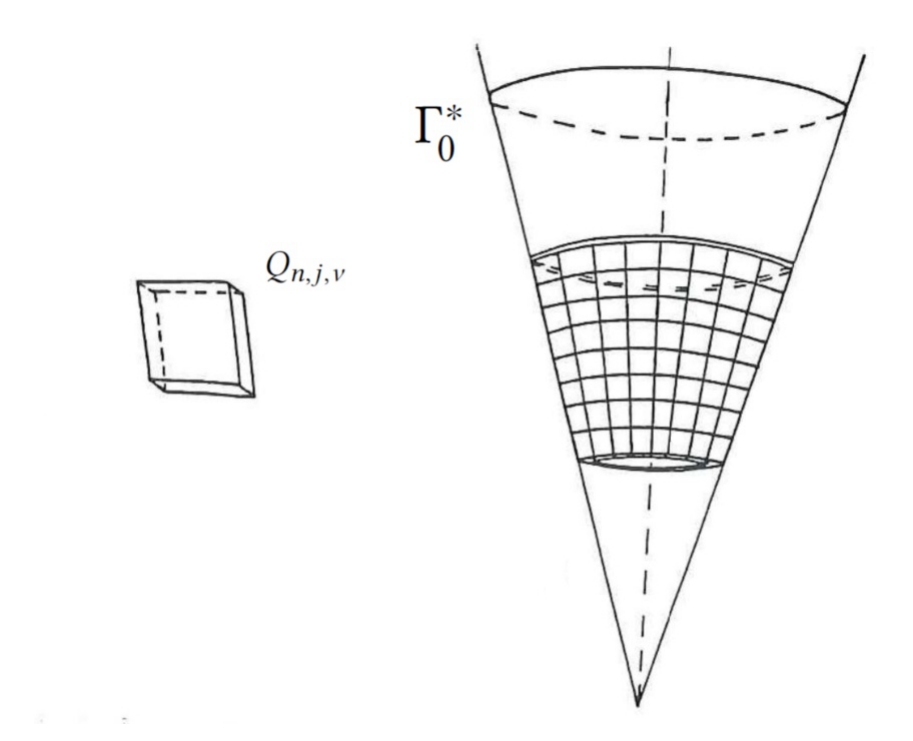
\includegraphics[width=0.42\textwidth]{figs/fig-5-4.png}
\caption{瓦片 $Q_{n,j,\nu}$.}
\label{fig:5.4}
\end{figure}

现在把 $\Gamma_0^*$ 分成 $\delta^{-1/2} \times \delta^{-1/2}$ 个瓦片 $Q_{0,j,\nu}$，其中 $Q_{0,j,\nu}$ 是尺寸 $\delta \times \delta^{1/2} \times \delta^{1/2}$ 的瓦片（板），由 $\Gamma_0^*$ 中高度 $1 + j\delta^{1/2} \leq z \leq 1 + (j+1)\delta^{1/2}$、角方向 $\delta^{1/2}\nu \leq \theta \leq \delta^{1/2}(\nu+1)$ 的点组成.

一旦得到 $\Gamma_0^*$ 的分解，就得到 $\Gamma_n^*$，并由齐性，得到 $\Gamma_n^*$ 到瓦片的类似分解. 这样，$\Gamma_n^*$ 将被分成 $\delta^{-1/2} \times \delta^{-1/2}$ 块 $Q_{n,j,\nu}$，其中 $Q_{n,j,\nu}$ 是尺寸 $2^n \delta \times 2^n \delta^{1/2} \times 2^n \delta^{1/2}$ 的瓦片，位于高度 $2^n + 2^n j \delta^{1/2} \leq z \leq 2^n + 2^n (j+1) \delta^{1/2}$、角方向 $\delta^{1/2}\nu \leq \theta \leq \delta^{1/2}(\nu+1)$. 为便于计算，我们可以假设 $Q_{n,j,\nu}$ 是适应于曲面的矩形瓦片. 见图~\ref{fig:5.4}.

令
\begin{align*}
  \Gamma^{*}=\bigcup_{n}\Gamma_{n}^{*},
\end{align*}
并称 $\varphi_{n,j,\nu}$ 为 $Q_{n,j,\nu}$ 的示性函数.

为证明不等式 \eqref{eq:5.4}，在去奇异化测度的过程中，只须考虑
\begin{align*}
  \lim_{\delta\rightarrow 0}\left(\frac{1}{\delta}\int_{\Gamma^{*}}|\widehat{f}(\xi)|^{q}\frac{\mathrm{d}\xi}{|\xi|^{2}}\right)^{1/q}
  \leq C\left\|f\right\|_{p},
\end{align*}
而为了对偶地证明这个不等式，只须取在每个瓦片上为常数的函数
\begin{align*}
  g(\xi)=\sum_{n,j,\nu}a_{n,j,\nu}\varphi_{n,j,\nu}(\xi),
\end{align*}
使对每个足够小的 $\delta > 0$,
\begin{equation}\label{eq:5.5}
  \Big\|\sum_{n,j,\nu}\frac{a_{n,j,\nu}}{2^{2n/q}}\widehat{\varphi}_{n,j,\nu}\Big\|_{p'}
  \leq C\delta^{1/q}\Big\|\sum_{n,j,\nu}a_{n,j,\nu}\varphi_{n,j,\nu}\Big\|_{q'},
\end{equation}
其中 $p'$ 与 $q'$ 分别是 $p$ 与 $q$ 的对偶指数.

由于只有极限情形 $\delta \to 0$ 有意义，我们考虑锥的任意固定部分 $2^{-M} \leq z \leq 2^M$，并将对固定的 $M$、在 $\delta$ 足够小时以与 $M$ 无关的界证明 \eqref{eq:5.5}.

于是取 $|n| > M$ 时 $a_{n,j,\nu} = 0$. 还取满足
\begin{align*}
  |n-m|\leq|\log_{2}\delta|/2
\end{align*}
的 $\delta$，因为这在几何上意味着（例如若 $m \leq n$）$\Gamma_m^*$ 的直径小于 $\Gamma_n^*$ 中每个瓦片. 这对随后的计算是必要的.

由于 $p' > 4$，可以对 \eqref{eq:5.5} 的左端应用 Hausdorff--Young 定理，其中 $1/s + 2/p' = 1$；则
\begin{align*}
  &\quad\left(\int\Big|\sum_{n,j,\nu}\frac{a_{n,j,\nu}}{2^{2n/q}}\widehat{\varphi}_{n,j,\nu}(\xi)\Big|^{p'}\mathrm{d}\xi\right)^{1/p'}\\
  &=\Big(\int\Big|\sum_{n,m}\sum_{j,k}\sum_{\nu,\mu}\frac{a_{n,j,\nu}a_{m,k,\mu}}{2^{2n/q}2^{2m/q}}
   \widehat{\varphi}_{n,j,\nu}(\xi)\cdot\widehat{\varphi}_{m,k,\mu}(\xi)\Big|^{p'/2}\mathrm{d}\xi\Big)^{(2/p')\cdot 1/2}\\
  &\leq\Big(\int\Big|\sum_{n,m}\sum_{j,k}\sum_{\nu,\mu}\frac{a_{n,j,\nu}a_{m,k,\mu}}{2^{2n/q}2^{2m/q}}
   \varphi_{n,j,\nu}*\varphi_{m,k,\mu}(x)\Big|^{s}\mathrm{d}x\Big)^{1/2s}\\
  &\leq C\Big(\int\Big|\sum_{m\leq n}\sum_{j,k}\sum_{\nu,\mu}\frac{a_{n,j,\nu}a_{m,k,\mu}}{2^{2n/q}2^{2m/q}}
   \varphi_{n,j,\nu}*\varphi_{m,k,\mu}(x)\Big|^{s}\mathrm{d}x\Big)^{1/2s}\\
  &\leq C\Big[\sum_{r=n-m\geq 0}\Big(\int\Big|\sum_{n}\sum_{j,k}\sum_{\nu,\mu}\frac{a_{n,j,\nu}a_{m,k,\mu}}{2^{2n/q}2^{2m/q}}
   \varphi_{n,j,\nu}*\varphi_{m,k,\mu}(x)\Big|^{s}\mathrm{d}x\Big)^{1/s}\Big]^{1/2}\\
  &=\Big[\sum_{r\geq 0}A_{r}\Big]^{1/2},
\end{align*}
其中对固定的 $r \geq 0$，$A_r$ 是上面括号中的表达式，其中一旦取定 $n$，就取 $m = n - r$.

还要注意，因为我们处于锥的固定部分 $2^{-M} \leq z \leq 2^M$，有 $r \leq |\log_2 \delta|/2$.

证明通过仔细分析被积函数中的不同项进行. 为此，需要估计支集的大小以及它们如何重叠.

$z$-坐标的作用体现在竖直重叠，而水平重叠用于研究 $\R^{2}$ 中不同半径圆周上测度 $f(\theta)\,\mathrm{d}\theta$ 的卷积.

为估计 $A_{r}$，如下面的计算所示: 若 $m$ 接近 $n$，则重叠小、尺寸大；但若 $m$ 远离 $n$，则重叠增大、尺寸减小. 妙处在于两者恰好互相补偿.

为度量竖直重叠，若 $m \leq n$，在 $\Gamma_m^*$ 中考虑 $2^m/(\delta^{1/2}2^n)$ 个环 $\Gamma_{m,l}^*$，其中 $\Gamma_{m,l}^*$ 是高度 $\delta^{1/2}2^n$ 的环，由并 $\bigcup_{k,\mu} Q_{m,k,\mu}$ 得到，$\mu$ 取遍所有角方向，$k$ 满足
\begin{align*}
  \delta^{1/2}2^{n}l\leq\delta^{1/2}2^{m}k\leq\delta^{1/2}2^{n}(l+1).
\end{align*}
于是
\begin{align*}
  \left[\Gamma_{m,l}^{*}+\supp(\varphi_{n,j,\nu})\right]
  \cap\left[\Gamma_{m,l'}+\supp(\varphi_{n,j',\nu'})\right]\neq\emptyset
\end{align*}
当 $l + j = l' + j'$ 时成立，而若 $l + j \neq l' + j'$，则此交集具有与 $\delta$ 无关的有限重叠.

由此，固定 $n, m$，$\Gamma_{m,l}^{*}+\supp(\varphi_{n,j,\nu})$ 中的一点至多属于 $2^{m}/(\delta^{1/2}2^{n})$ 个这类和.

由于
\begin{align*}
  \supp\left(\varphi_{n,j,\nu}*\sum_{\mu}\varphi_{m,k,\mu}\right)
  \cap\supp\left(\varphi_{n,j,\nu}*\sum_{\mu}\varphi_{m,k',\mu}\right)\neq\emptyset
\end{align*}
对所有满足 $\supp(\sum_\mu \varphi_{m,k,\mu}) \subset \Gamma_{m,l}^*$ 且 $\supp(\sum_\mu \varphi_{m,k',\mu}) \subset \Gamma_{m,l}^*$ 的 $k, k'$ 成立，而这种指标共有 $2^n/2^m$ 个，于是 $\supp(\varphi_{n,j,\nu} * \sum_\mu \varphi_{m,k,\mu})$ 中的一点至多属于
\begin{align*}
  \left(\frac{2^{m}}{\delta^{1/2}2^{n}}\right)\cdot\left(\frac{2^{n}}{2^{m}}\right)=\delta^{-1/2}
\end{align*}
个这一类的支集.

这就提供了竖直重叠. 于是有
\begin{equation}\label{eq:5.7}
  \begin{aligned}
  \sum_{r}A_{r}
  &=\sum_{\substack{0\leq r\leq\frac{1}{2}|\log_{2}\delta|\\ r=n-m}}
   \left\{\int\left|\sum_{n}\sum_{j,k}\sum_{\nu,\mu}\frac{a_{n,j,\nu}a_{m,k,\mu}}{2^{2n/q}2^{2m/q}}
   \varphi_{n,j,\nu}*\varphi_{m,k,\mu}(x)\right|^{s}\mathrm{d}x\right\}^{1/s}\\
  &\leq C\sum_{\substack{n-m\leq|\log_{2}\delta|\\ m\leq n}}
   \left\{\sum_{n}\sum_{j,k}\frac{\delta^{-(s-1)/2}}{2^{2ns/q}2^{2ms/q}}
   \Big|\Big(\sum_{\nu}a_{n,j,\nu}\varphi_{n,j,\nu}\Big)
   *\Big(\sum_{\mu}a_{m,k,\mu}\varphi_{m,k,\mu}\Big)(x)\Big|^{s}\mathrm{d}x\right\}^{1/s}.
  \end{aligned}
\end{equation}

现在继续估计水平重叠. 必须记住，若两个支集 $Q_{n,j,\nu}$ 与 $Q_{m,k,\mu}$ 的角距离 $|\nu - \mu|$ 很小，则和 $Q_{n,j,\nu} + Q_{m,k,\mu}$ 的尺寸将与 $Q_{n,j,\nu}$ 一样大，且与其他支集会有可观的重叠. 角距离大时则相反.

一旦固定了高度 $j$ 与 $k$，为研究该情形，只须观察它在高度
\begin{align*}
  2^{n}+2^{m}+j\delta^{1/2}2^{n}+k\delta^{1/2}2^{m}
\end{align*}
处垂直于锥轴的截面 $S_{j,k}$ 上的表现，因为 $\supp(\varphi_{n,j,\nu}*\sum_{\mu}\varphi_{m,k,\mu})$ 位于这个高度，而最终的和 $Q_{n,j,\nu}+Q_{m,k,\mu}$ 将由其截面 $S_{j,k}$ 沿 $Q_{n,j,\nu}$ 的竖直方向平移得到.

\begin{figure}[htbp]
\centering
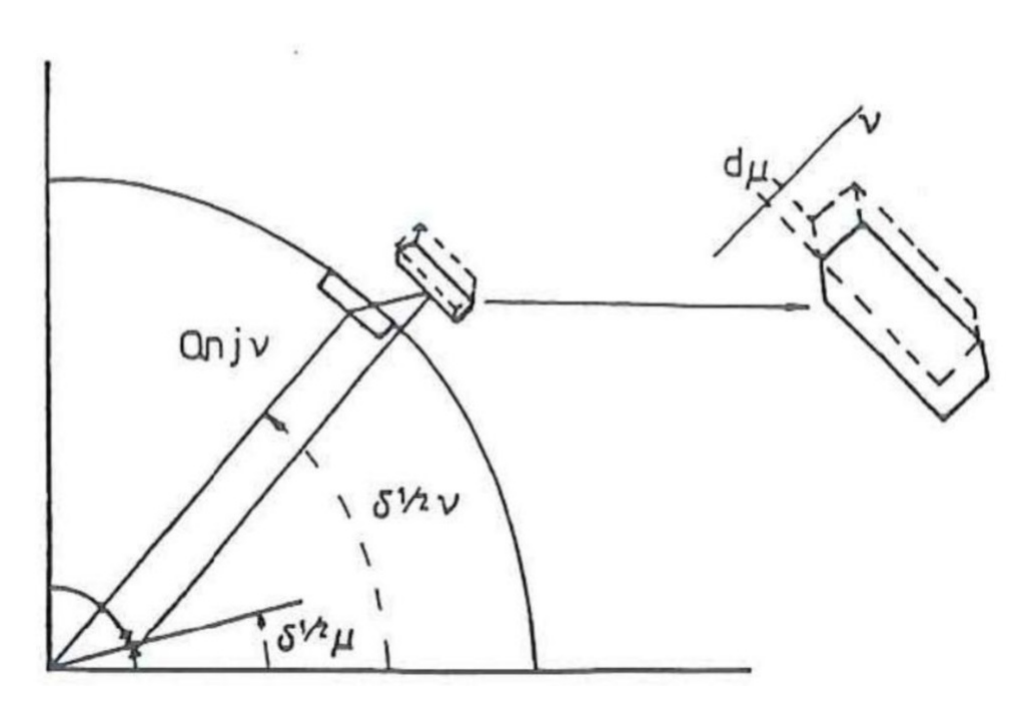
\includegraphics[width=0.52\textwidth]{figs/fig-5-5.png}
\caption{瓦片的和集.}
\label{fig:5.5}
\end{figure}

在 $S_{j,k}$ 平面中，$\supp(\varphi_{n,j,\nu} * \varphi_{m,k,\mu})$ 以点
\begin{align*}
  2^{n}\left(1+\delta^{1/2}j\right)e^{\pi\nu i/2}
  +2^{m}\left(1+\delta^{1/2}k\right)e^{\pi\mu i/2}
\end{align*}
为中心，本质上像一个长 $2^n \delta^{1/2}$、宽
\begin{align*}
  \delta^{1/2}2^{n}+\delta^{1/2}2^{m}\sin\bigl((|\nu-\mu|+1)\delta^{1/2}\bigr)
\end{align*}
的块. 此外，$\supp(\varphi_{n,j,\nu} * \varphi_{m,k,\mu})$ 与 $\supp(\varphi_{n,j,\nu} * \varphi_{m,k,\mu+1})$ 相距平移
\begin{align*}
  \delta^{1/2}2^{m}\sin(|\nu-\mu|\delta^{1/2})\simeq\delta2^{m}|\nu-\mu|,
\end{align*}
这在 $\nu$ 方向上投影即可看出.

为度量卷积 $\varphi_{n,j,\nu} * \varphi_{m,k,\mu}$ 重叠的个数，区分下面两种情形:

情形 (i). $|\nu - \mu| + 1 \leq 2^{n-m}$.

此时，一点至多属于 $N$ 个不同的支集，其中 $N$ 满足
\begin{align*}
  \delta2^{m}|\nu-\mu|+\delta2^{m}(|\nu-\mu|-1)+\cdots+\delta2^{m}(|\nu-\mu|-N)\leq\delta2^{n},
\end{align*}
即 $N \leq 2^{n-m}/(|\nu - \mu| + 1)$.

此外,
\begin{align*}
  |\supp(\varphi_{n,j,\nu}\ast\varphi_{m,k,\mu})|\simeq|\supp(\varphi_{n,j,\nu})|=\delta^{2}2^{3n},
\end{align*}
以及
\begin{align*}
  \|\varphi_{n,j,\nu}\ast\varphi_{m,k,\mu}\|_{\infty}\simeq|\supp(\varphi_{m,k,\mu})|=\delta^{2}2^{3m}.
\end{align*}
因此
\begin{align*}
  \int|\varphi_{n,j,\nu}\ast\varphi_{m,k,\mu}(x)|^{s}\mathrm{d}x
  \leq C\delta^{2s+2}2^{3ms}2^{3n}.
\end{align*}

情形 (ii). $\left|\nu - \mu\right| + 1 \geq 2^{n-m}$.

则当 $\mu$ 变化时 $\supp(\varphi_{n,j,\nu} * \varphi_{m,k,\mu})$ 有有限重叠，且
\begin{align*}
  |\supp(\varphi_{n,j,\nu}*\varphi_{m,k,\mu})|
  &\leq C\delta^{2}2^{2n}2^{m}(|\nu-\mu|+1),\\
  \|\varphi_{n,j,\nu}*\varphi_{m,k,\mu}\|_{\infty}
  &\leq C\delta^{2}2^{n}2^{2m}/(|\nu-\mu|+1).
\end{align*}
于是,
\begin{align*}
  \int\left|\varphi_{n,j,\nu}*\varphi_{m,k,\mu}(x)\right|^{s}\mathrm{d}x
  \leq C\frac{\delta^{2s+2}2^{n(2+s)}2^{m(2s+1)}}{\left(|\nu-\mu|+1\right)^{s-1}}.
\end{align*}

然后，用 (i) 与 (ii) 可以把 \eqref{eq:5.7} 写成
\begin{align*}
  \leq C\sum_{\substack{n-m\leq|\log_{2}\delta|\\ m\leq n}}\Bigg\{&\sum_{n}\sum_{j,k}\frac{\delta^{-(s-1)/2}}{2^{2ns/q}\;2^{2ms/q}}\\
  \times\Big[&\sum_{|\nu-\mu|+1\leq 2^{n-m}}\Big(\frac{2^{n-m}}{|\nu-\mu|+1}\Big)^{s-1}\delta^{2s+2}\;2^{3n}\;2^{3ms}|a_{n,j,\nu}|^{s}|a_{m,k,\mu}|^{s}\\
  &+\sum_{|\nu-\mu|+1\geq 2^{n-m}}\delta^{2s+2}\;2^{n(2+s)}\;2^{m(2s+1)}
   \frac{|a_{n,j,\nu}|^{s}|a_{m,k,\mu}|^{s}}{(|\nu-\mu|+1)^{s-1}}\Big]\Bigg\}^{1/s}\\
  \leq C\sum_{\substack{n-m\leq|\log_{2}\delta|\\ m\leq n}}\Bigg\{\sum_{n}\sum_{j,k}
  &\frac{\delta^{-(s-1)/2}\;\delta^{2s+2}\;2^{m(2s+1)}\;2^{n(2+s)}}{2^{2ns/q}\;2^{2ms/q}}\\
  &\times\sum_{\nu,\mu}\frac{|a_{n,j,\nu}|^{s}|a_{m,k,\mu}|^{s}}{(|\nu-\mu|+1)^{s-1}}\Bigg\}^{1/s},
\end{align*}
再由分数积分论证,
\begin{align*}
  \sum_{\nu,\mu}\frac{\left|a_{n,j,\nu}\right|^{s}\left|a_{m,k,\mu}\right|^{s}}{(|\nu-\mu|+1)^{s-1}}
  \leq C\left(\sum_{\nu}\left|a_{n,j,\nu}\right|^{2s/(3-s)}\right)^{(3-s)/2}
  \left(\sum_{\mu}\left|a_{m,k,\mu}\right|^{2s/(3-s)}\right)^{(3-s)/2}.
\end{align*}
因此，\eqref{eq:5.7} 为
\begin{align*}
  &\leq C\sum_{\substack{n-m\leq|\log_{2}\delta|\\ m\leq n}}
   \delta^{(3s-3)/s}2^{-|n-m|(s-1)/s}\\
  &\quad\cdot\left\{\sum_{n}
   \left(\sum_{j,\nu}|a_{n,j,\nu}|^{2s/(3-s)}\delta^{2}2^{3n}\right)^{(3-s)/2}
   \left(\sum_{k,\mu}|a_{m,k,\mu}|^{2s/(3-s)}\delta^{2}2^{3m}\right)^{(3-s)/2}\right\}^{1/s}\\
  &\leq C\delta^{(3s-3)/s}
   \left(\sum_{\substack{n-m\leq|\log_{2}\delta|\\ m\leq n}}2^{-|n-m|(s-1)/s}\right)
   \left(\sum_{n,j,\nu}|a_{n,j,\nu}|^{2s/(3-s)}\delta^{2}2^{3n}\right)^{(3-s)/s},
\end{align*}
但
\begin{align*}
  \sum_{\substack{n-m\leq|\log_2\delta|\\ m\leq n}}2^{-|n-m|(s-1)/s}\leq C,
\end{align*}
于是我们证明了
\begin{align*}
  \sum_{r\geq 0}A_{r}\leq C\delta^{(3s-3)/s}
  \Big(\sum_{n,j,\nu}|a_{n,j,\nu}|^{2s/(3-s)}\delta^{2}2^{3n}\Big)^{(3-s)/s}.
\end{align*}
现在注意到 $(3s - 3)/2s = 1/q$ 且 $(3 - s)/2s = 1/q'$，最终可以得出
\begin{align*}
  \Big\|\sum_{n,j,\nu}\frac{a_{n,j,\nu}}{2^{2n/q}}\widehat{\varphi}_{n,j,\nu}\Big\|_{p'}
  \leq C\left(\sum_{r}A_{r}\right)^{1/2}
  \leq C\delta^{1/q}\Big\|\sum_{n,j,\nu}a_{n,j,\nu}\varphi_{n,j,\nu}\Big\|_{q'},
\end{align*}
这就是不等式 \eqref{eq:5.5}.
\end{proof}

限制定理已被推广到 $\R^n$ 中曲线的情形（见，例如，\cite{b114,b125}），当 $n \geq 3$ 时对超曲面也有一些部分结果. 但它们的证明，见 \cite{b99,b127,b128}，并不符合本章的``至上主义''观点.

\section{沿平面曲线的希尔伯特变换}

Calderón 与 Zygmund 开创的奇异积分的实变理论已以若干不同方式被推广.

其中一种推广是奇异积分算子
\begin{align*}
  H f(x)=\mathrm{p.v.}\int_{-\infty}^{\infty}f(x-\Gamma(t))\frac{\mathrm{d}t}{t},
\end{align*}
其中 $\Gamma\colon \R \to \R^n$，$n \geq 2$，是过原点的曲线: $\Gamma(0) = 0$. 这个对象——称为沿曲线 $\Gamma$ 的希尔伯特变换——出现在抛物型微分算子的研究以及齐性空间的调和分析中.

这些对象也是傅里叶变换的乘子，因而可以用公式
\begin{align*}
  \widehat{H f}(\xi)=\widehat{f}(\xi)m(\xi)
\end{align*}
定义，其中
\begin{align*}
  m(\xi)=\mathrm{p.v.}\int_{-\infty}^{\infty}\exp(i\xi\cdot\Gamma(t))\frac{\mathrm{d}t}{t}.
\end{align*}
与普通希尔伯特变换的情形（那里 Hardy--Littlewood 极大函数是控制其行为的正算子）类似，可以定义与这些奇异积分相伴的极大算子:
\begin{equation}\label{eq:5.8}
  M f(x)=\sup_{h>0}\frac{1}{2h}\int_{-h}^{h}\left|f(x-\Gamma(t))\right|\mathrm{d}t,
\end{equation}
\begin{equation}\label{eq:5.9}
  H^{*}f(x)=\sup_{\varepsilon>0}\Big|\int_{|t|\geq\varepsilon}f(x-\Gamma(t))\frac{\mathrm{d}t}{t}\Big|.
\end{equation}
人们可能问的第一个自然问题是: 应当对曲线 $\Gamma$ 施加什么条件，才能使 $H$，$H^*$ 与 $M$ 在某个或所有空间 $L^p(\R^n)$ 上有界? 在一系列论文中，A.~Nagel，E.~Stein，S.~Wainger 等人 \cite{b120,b121} 获得了涉及 $\Gamma$ 曲率某种``正性''的结果，利用了它所蕴含的乘子 $m(\xi)$ 的衰减. 证明由复插值方法的巧妙运用，连同涉及某些平方函数的 Tauber 型论证完成. 在 \cite{b121} 中观察到，对 $\R^2$ 中凸曲线 $\Gamma(t) = (t, \gamma(t))$（$\gamma(0) = \gamma'(0) = 0$），存在 $H$ 在 $L^2(\R^2)$ 有界的充要条件: 当 $\gamma$ 为偶函数（相应地，奇函数）时，条件是 $\gamma'(t)$（相应地，$h(t) = t\gamma'(t) - \gamma(t)$）必须具有倍时性质，即对某个固定常数 $C$ 与每个 $t > 0$，$\gamma'(Ct) \geq 2\gamma'(t)$（相应地，$h(Ct) \geq 2h(t)$）. $L^p$-估计的范围在 \cite{b111} 中从 $L^2$ 推广到 $L^p$，$4/3 < p < 4$.

考虑 $\R^2$ 中的 $C^1$ 曲线 $\Gamma = \{(t, \gamma(t)): -\infty < t < +\infty\}$，$\gamma(0) = \gamma'(0) = 0$，具有如下性质:

(a) $\gamma$ 是双凸的，即 $|\gamma'(t)|$ 在 $(-\infty, 0)$ 上递减，在 $(0, +\infty)$ 上递增.

(b) $\gamma$ 具有倍时性，即存在常数 $C > 1$，使 $|\gamma'(Ct)| \geq 2|\gamma'(t)|$.

(c) $\gamma$ 是平衡的，意思如下: 存在 $k > 1$，使对每个 $t > 0$ 有 $|\gamma(k^{-1}t)| \leq |\gamma(-t)| \leq |\gamma(kt)|$.

\begin{theorem}\label{thm:5.21}
在关于曲线的假设 (a)，(b) 与 (c) 之下，奇异积分 $H$ 与极大函数 $M$ 和 $H^*$ 是 $L^p(\R^2)$ 上的有界算子，对每个 $p$，$1<p<\infty$ 成立.
\end{theorem}

$M$ 与 $H^{*}$ 有界性的直接推论是:

\begin{corollary}\label{cor:5.22}
对每个 $f \in L^p(\R^2)$，$1 < p < \infty$,
\begin{align*}
  &\lim_{\varepsilon\rightarrow 0}\frac{1}{2\varepsilon}\int_{-\varepsilon}^{\varepsilon}f(x-\Gamma(t))\,\mathrm{d}t=f(x)\quad\text{a.e.},\\
  &\lim_{\varepsilon\rightarrow 0}\int_{|t|>\varepsilon}f(x-\Gamma(t))\frac{\mathrm{d}t}{t}=H f(x)\quad\text{a.e.}
\end{align*}
\end{corollary}

定理 5.21 对平面凸曲线沿曲线的希尔伯特变换的性质给出了相当完整的分析. 对每个固定的 $p$，$1 < p < \infty$，若曲线为偶，则倍时性质是 $L^p$-有界性的充要条件. 同样，对双凸曲线，平衡条件对 $H$ 的 $L^2$-有界性是必要的，正如后面 5.7.5 节所证明的. 对这样的曲线，不能只获得 $L^p(\R^2)$ 中某些 $p$ 的希尔伯特变换有界性而不获得全范围 $1 < p < \infty$；这反过来解释了该理论的成功，与球面求和乘子分析中的情形形成对照.

\subsection{算子的分解与证明梗概}

所有 $L^p$ 估计都将对 $f \in \mathcal{S}(\R^2)$ 证明，再由连续性扩张. 定义奇异测度 $M_k$ 与 $h_k$（$k \in \Z$），使
\begin{align*}
  \widehat{M}_{k}(\xi,\eta)=\int_{1\leq|t|\leq 2}\exp\left\{i(2^{k}t\xi+\gamma(2^{k}t)\eta)\right\}\mathrm{d}t,
\end{align*}
\begin{align*}
  \widehat{h}_{k}(\xi,\eta)=\int_{1\leq|t|\leq 2}\exp\left\{i(2^{k}t\xi+\gamma(2^{k}t)\eta)\right\}\frac{\mathrm{d}t}{t},
\end{align*}
并考虑我们的算子的下列基本分解:
\begin{equation}\label{eq:5.10}
  Mf(x)\simeq\sup_{k}|M_{k}*f(x)|,
\end{equation}
\begin{equation}\label{eq:5.11}
  H f(x)=\sum_{k=-\infty}^{\infty}h_{k}*f(x),
\end{equation}
\begin{equation}\label{eq:5.12}
  H^{*}f(x)\simeq\sup_{k}\Big|\sum_{n>k}h_{n}*f(x)\Big|.
\end{equation}
我们还将使用下列平方函数:
\begin{equation}\label{eq:5.13}
  G f(x)=\Big(\sum_{k=-\infty}^{\infty}|\widetilde{M}_{k}f(x)|^{2}\Big)^{1/2},
\end{equation}
其中
\begin{align*}
  \widehat{\widetilde{M}_{k}f}(\xi,\eta)=\left[\widehat{M}_{k}(\xi,\eta)-\widehat{\Phi}(2^{k}\xi)\widehat{M}_{k}(0,\eta)\right]\widehat{f}(\xi,\eta),
\end{align*}
$\Phi$ 是 Schwartz 类中满足 $\Phi(0) = 1$ 的适当函数.

极大函数 $Mf$ 的有界性证明基于如下策略: 有逐点控制 $M f(x) \leq G f(x) + f^*(x)$，其中 $f^*$ 表示 $f$ 的强极大函数. 首先用 Plancherel 定理证明 $Gf$ 的 $L^2$-有界性. 这蕴含 $Mf$ 的同样结果，再由如今众所周知的基于向量值不等式与频率空间特殊 Littlewood--Paley 分解的论证，蕴含平方函数 $Gf$ 的 $L^p$ 估计（$4/3 < p < 4$）. 一般地，$M$ 的 $L^p$ 估计蕴含 $G$ 的 $L^q$ 估计，其中 $|1/q - 1/2| < 1/(2p)$；因此，bootstrap 论证将给出整个 $1 < p < \infty$ 的范围.

曲线的倍时条件将用于定义角 Littlewood--Paley 分解. 为简单起见，假设倍时常数为 $C = 2$. 于是考虑角区域
\begin{align*}
  \Delta_{k}^{\pm}=\Big\{(\xi,\eta):
  \frac{1}{2}|\gamma^{\prime}(\pm 2^{k})|<\frac{|\xi|}{|\eta|}<2|\gamma^{\prime}(\pm 2^{k+1})|\Big\},\qquad k\in\Z.
\end{align*}
结果表明 $\{\Delta_k^+\}_{-\infty}^{\infty}$ 是 $\R^2$ 的缺项分解，具有有限重叠: 若 $|k - h| \geq 3$ 则 $\Delta_h^+ \cap \Delta_k^+ = \emptyset$，对 $\{\Delta_k^-\}$ 亦然.

\subsection{极大算子与平方函数}

设 $\Delta_{k} = \Delta_{k}^{+} \cup \Delta_{k}^{-}$，定义投影算子 $T_{k}$:
\begin{align*}
  \widehat{(T_{k}f)}=\widehat{f}\chi_{\Delta_{k}},\qquad k\in\Z.
\end{align*}

\begin{lemma}\label{lem:5.23}
对每个 $p$，$1 < p < \infty$，有
\begin{equation}\label{eq:5.14}
  \left\|\Big(\sum_{k}\left|T_{k}f\right|^{2}\Big)^{1/2}\right\|_{p}\leq c_{p}\left\|f\right\|_{p},
\end{equation}
\begin{equation}\label{eq:5.15}
  \Big\|\sum_{k}T_{k}f_{k}\Big\|_{p}\leq c_{p}\Big\|\Big(\sum_{k}|f_{k}|^{2}\Big)^{1/2}\Big\|_{p},
\end{equation}
\begin{equation}\label{eq:5.16}
  \left\|\sup_{k}\left|\sum_{n\geq k}T_{n}f\right|\right\|_{p}\leq c_{p}\left\|f\right\|_{p}.
\end{equation}
\end{lemma}

不等式 \eqref{eq:5.14} 如今众所周知（参考文献见 \cite{b98}），\eqref{eq:5.15} 是其对偶形式；\eqref{eq:5.16} 由 \eqref{eq:5.14} 按证明傅里叶级数缺项收敛的同样方式得出.

\begin{lemma}\label{lem:5.24}
算子
\begin{align*}
  \Gamma f(x)=\sup_{h>0}\frac{1}{2h}\int_{-h}^{h}\left|f(x-\gamma(t))\right|\mathrm{d}t
\end{align*}
是 $L^p(\R)$（$1 < p < \infty$）上的有界算子.
\end{lemma}

证明由于 $\gamma'$ 的单调性是显然的:
\begin{align*}
  \frac{1}{h}\int_{0}^{h}f(x-\gamma(t))\,\mathrm{d}t
  &=\frac{1}{h}\int_{0}^{\gamma(h)}f(x-u)\frac{\mathrm{d}u}{\gamma'(\gamma^{-1}(u))}\\
  &=\int_{0}^{c}f(x-u)\varphi(u)\,\mathrm{d}u\leq f^{*}(x),
\end{align*}
（Hardy--Littlewood 极大函数），因为 $\varphi(u)$ 非负、递减且满足 $\int_{0}^{c}\varphi(u)\,\mathrm{d}u = 1$. 对区间 $[-h, 0]$ 上的平均，同样的论证成立.

\begin{lemma}\label{lem:5.25}
设 $\Phi \in \mathcal{S}(\R)$ 满足 $\chi_{[-1,1]} \leq \Phi \leq \chi_{[-2,2]}$. 则
\begin{align*}
  \left|\widehat{M}_{k}(\xi,\eta)-\widehat{\Phi}(2^{k}\xi)\widehat{M}_{k}(0,\eta)\right|
  \leq C\min\bigl(2^{k}|\xi|,(2^{k}|\xi|)^{-1}\bigr),
\end{align*}
对所有 $(\xi,\eta)\notin\Delta_{k}$ 成立. 对 $\widehat{h}_{k}(\xi,\eta)$ 代替 $\widehat{M}_{k}(\xi,\eta)$，同样的估计成立.
\end{lemma}

\begin{proof}
$2^k|\xi| \leq 1$ 情形的估计是平凡的，因为 $M_k$ 是支于 $\{(x_1, x_2) : |x_1| \leq 2^{k+1}\}$ 的测度. 对 $2^k|\xi| > 1$，用 van der Corput 引理:
\begin{align*}
  \widehat{M}_{k}(\xi,\eta)=\int_{1}^{2}e^{i g_{k}(t)}\,\mathrm{d}t+\int_{1}^{2}e^{i l_{k}(t)}\,\mathrm{d}t,
\end{align*}
其中
\begin{align*}
  |g_{k}^{\prime}(t)|=|2^{k}(\xi+\gamma^{\prime}(2^{k}t)\eta)|,\qquad
  |l_{k}^{\prime}(t)|=|2^{k}(\xi+\gamma^{\prime}(-2^{k}t)\eta)|.
\end{align*}
若 $|\xi| \geq 2|\eta|\cdot|\gamma'(2^{k+1})|$，则 $|g_k'(t)| \geq 2^{k-1}|\xi|$. 若 $|\xi| \leq \frac{1}{2}|\eta|\cdot|\gamma'(2^k)|$，则也有 $|g_k'(t)| \geq 2^{k-1}|\gamma'(2^k t)|\cdot|\eta| \geq 2^k|\xi|$；对 $l'_k$ 情形类似. 最后，这四种情形的补集正对应点 $(\xi, \eta) \in \Delta_k$. 对 $\widehat{h}_k(\xi, \eta)$ 的证明本质相同.
\end{proof}

假设 $U_k f = U_k * f$ 是在 $L^\infty(\R^n)$ 上一致有界的正算子序列，考虑 $U^* f(x) = \sup_k |U_k * f(x)|$.

\begin{lemma}\label{lem:5.26}
若 $U^* f(x) = \sup_k |U_k * f(x)|$ 在 $L^q(\R^n)$ 上有界，则
\begin{align*}
  \left\|\Big(\sum_{k}|U_{k}f_{k}|^{2}\Big)^{1/2}\right\|_{p}
  \leq c_{p}\left\|\Big(\sum_{k}|f_{k}|^{2}\Big)^{1/2}\right\|_{p}
\end{align*}
对 $|1/p - 1/2| = 1/(2q)$ 成立.
\end{lemma}

这是众所周知的结果，在这里陈述只是为了厘清定理 5.21 证明的表述. 极大函数估计的证明依赖于下面这个条件性质的命题.

\begin{lemma}\label{lem:5.27}
假设对某个 $q$ 有 $\|Mf\|_q \leq C\|f\|_q$. 则对所有满足 $|1/p - 1/2| < 1/(2q)$ 的 $p$，有不等式
\begin{align*}
  \left\|G f\right\|_{p}\leq C_{p}\left\|f\right\|_{p},
\end{align*}
其中 $G$ 由 \eqref{eq:5.13} 定义.
\end{lemma}

\begin{proof}
回忆 $T_{k}f = \chi_{\Delta_{k}}\cdot\widehat{f}$，写
\begin{align*}
  f^{k}=f-T_{k}f,
\end{align*}
以及
\begin{align*}
  S_{k}f=\widehat{f}\cdot\chi\{(\xi,\eta):2^{k}\leq|\xi|\leq 2^{k+1}\}.
\end{align*}
则
\begin{align*}
  G f\leq\Big(\sum_{k}|\widetilde{M}_{k}*T_{k}f|^{2}\Big)^{1/2}
  +\Big(\sum_{k}|\widetilde{M}_{k}*f^{k}|^{2}\Big)^{1/2}=\mathbf{I}+\mathbf{II}.
\end{align*}
现在注意，由假设与引理 5.24，$\sup_k(|\widetilde{M}_k|*f)$ 是 $L^q$ 上的有界算子. 因此
\begin{align*}
  \left\|\mathrm{I}\right\|_{p}\leq C_{p}\left\|\Big(\sum_{k}\left|T_{k}f\right|^{2}\Big)^{1/2}\right\|_{p}\leq C_{p}\left\|f\right\|_{p}
\end{align*}
由引理 5.26 与引理 5.23.

有
\begin{align*}
  \mathrm{II}=\Big(\sum_{k}\Big|\widetilde{M}_{k}*\Big(\sum_{j=-\infty}^{\infty}S_{j+k}f^{k}\Big)\Big|^{2}\Big)^{1/2}
  \leq\sum_{j}\Big(\sum_{k}|\widetilde{M}_{k}*S_{j+k}f^{k}|^{2}\Big)^{1/2}
  =\sum_{j}\mathrm{II}_{j}.
\end{align*}
我们将证明:
\begin{align*}
  \left\|\mathrm{II}_{j}\right\|_{2}\leq C2^{-\left|j\right|}\left\|f\right\|_{2},
  \qquad
  \left\|\mathrm{II}_{j}\right\|_{p_{0}}\leq C\left\|f\right\|_{p_{0}},
  \quad \left|\frac{1}{2}-\frac{1}{p_{0}}\right|=\frac{1}{2q}.
\end{align*}
插值，将得到
\begin{align*}
  \left\|\mathrm{II}\right\|_{p}\leq\sum_{j}\left\|\mathrm{II}_{j}\right\|_{p}
  \leq\sum_{j}C2^{-\theta\left|j\right|}\left\|f\right\|_{p}
  \leq C_{p}\left\|f\right\|_{p},
  \qquad \frac{1}{p}=\frac{1-\theta}{p_{0}}+\frac{\theta}{2}.
\end{align*}
对 $L^{2}$-不等式用 Plancherel 定理:
\begin{align*}
  \|\mathrm{II}_{j}\|_{2}^{2}
  &=\sum_{k}\int_{\substack{|\xi|\sim 2^{-j-k}\\ (\xi,\eta)\notin\Delta_{k}}}
   |\widehat{M}_{k}(\xi,\eta)-\widehat{\Phi}(2^{k}\xi)\widehat{M}_{k}(0,\eta)|^{2}|\widehat{f}(\xi,\eta)|^{2}\,\mathrm{d}\xi\,\mathrm{d}\eta\\
  &\stackrel{(\text{由引理~5.25})}{\leq}C\int|\widehat{f}(\xi,\eta)|^{2}(2^{-|j|})^{2}\,\mathrm{d}\xi\,\mathrm{d}\eta
  =C2^{-2|j|}\|f\|_{2}^{2}.
\end{align*}
最后,
\begin{align*}
  \|\mathrm{II}_{j}\|_{p_{0}}
  &\leq C_{p_{0}}\left\|\Big(\sum_{k}|S_{j+k}f^{k}|^{2}\Big)^{1/2}\right\|_{p_{0}}\\
  &\leq C_{p_{0}}\left\{\left\|\Big(\sum_{k}|S_{j+k}f|^{2}\Big)^{1/2}\right\|_{p_{0}}
   +\left\|\Big(\sum_{k}|S_{j+k}(T_{k} f)|^{2}\Big)^{1/2}\right\|_{p_{0}}\right\}\\
  &\leq C_{p_{0}}\left\{\|f\|_{p_{0}}+\left\|\Big(\sum_{k}|T_{k} f|^{2}\Big)^{1/2}\right\|_{p_{0}}\right\}
  \leq C_{p_{0}}\|f\|_{p_{0}}.
\end{align*}
\end{proof}

为完成极大算子定理的证明，使用控制
\begin{align*}
  Mf(x)\leq 2\sup_{k}|M_{k}*f(x)|
  \leq 2\sup_{k}|\widetilde{M}_{k}*f(x)|+2Nf(x)
  \leq 2Gf(x)+2Nf(x),
\end{align*}
其中 $N$ 是 $x_1$-变量的 Hardy--Littlewood 算子与 $x_2$-变量引理 5.24 的算子 $\Gamma$ 的复合. 现在可以应用 5.7.1 节勾画的 bootstrap 论证，给出对 $1 < p \leq \infty$ 的 $\|M f\|_p \leq C_p \|f\|_p$.

\subsection{奇异积分}

$Hf$ 的估计将基于与引理 5.27 类似的论证，连同算子 $h_k * f$ 被极大算子 $Mf$ 控制这一事实.

首先考虑 $\gamma(t)$ 为偶函数的情形，使 $\widehat{h}_{k}(0,\eta)=0$. 所用记号与引理 5.27 相同:
\begin{align*}
  H f=\sum_{k}h_{k}*T_{k}f+\sum_{k}h_{k}*f^{k}=H_{\mathrm{I}}f+H_{\mathrm{II}}f.
\end{align*}
利用引理 5.23 与 5.26，以及 $\sup_k |h_k| * f \leq M f$ 的事实，得到
\begin{align*}
  \left\|H_{\mathrm{I}}f\right\|_{p}
  &=\left\|\sum_{k}T_{k}(h_{k}*T_{k}f)\right\|_{p}
  \leq C_{p}\left\|\Big(\sum_{k}|h_{k}*T_{k}f|^{2}\Big)^{1/2}\right\|_{p}\\
  &\leq C_{p}\left\|\Big(\sum_{k}|T_{k}f|^{2}\Big)^{1/2}\right\|_{p}
  \leq C_{p}\left\|f\right\|_{p}.
\end{align*}
另一方面,
\begin{align*}
  |H_{\mathrm{II}}f|=\Big|\sum_{k}h_{k}*\sum_{j=-\infty}^{\infty}S_{j+k}f^{k}\Big|
  \leq\sum_{j}\Big|\sum_{k}h_{k}*S_{j+k}f^{k}\Big|
  =\sum_{j}|\mathrm{II}_{j}|.
\end{align*}
由于 $h_{k}(0,\eta)=0$，引理 5.25 与 Plancherel 定理给出
\begin{align*}
  \|\mathrm{II}_{j}\|_{2}^{2}
  &=\sum_{k}\int_{\substack{|\xi|\sim 2^{-j-k}\\ (\xi,\eta)\notin\Delta_{k}}}
   |\widehat{f}(\xi,\eta)|^{2}|\widehat{h}_{k}(\xi,\eta)|^{2}\,\mathrm{d}\xi\,\mathrm{d}\eta
  \leq C\int|\widehat{f}(\xi,\eta)|^{2}2^{-2|j|}\,\mathrm{d}\xi\,\mathrm{d}\eta\\
  &\leq C2^{-2|j|}\|f\|_{2}^{2}.
\end{align*}
在 $L^{p}$（$1 < p < \infty$）中有一致估计
\begin{align*}
  \|\mathrm{II}_{j}\|_{p}
  &=\Big\|\sum_{k}S_{j+k}(h_{k}*S_{j+k}f^{k})\Big\|_{p}
  \leq C_{p}\left\|\Big(\sum_{k}|h_{k}*(S_{j+k}f^{k})|^{2}\Big)^{1/2}\right\|_{p}\\
  &\leq C_{p}\left\|\Big(\sum_{k}|S_{j+k}f^{k}|^{2}\Big)^{1/2}\right\|_{p}
  \leq C_{p}\|f\|_{p},
\end{align*}
证明以插值和求等比级数结束.

对一般曲线的情形，分解
\begin{align*}
  h_{k}=\widetilde{h}_{k}+m_{k},
\end{align*}
其中，$\Phi$ 如前,
\begin{align*}
  \widehat{m}_{k}(\xi,\eta)=\widehat{\Phi}(2^{k}\xi)\cdot\widehat{h}_{k}(0,\eta).
\end{align*}
则 $h_{k}$ 的傅里叶变换满足与偶曲线情形相同的估计，即
\begin{align*}
  |\widehat{h}_{k}(\xi,\eta)|\leq C\min(2^{k}|\xi|,(2^{k}|\xi|)^{-1}),\qquad (\xi,\eta)\notin\Delta_{k},
\end{align*}
且 $\sup_k |\widetilde{h}_k| * f \leq M f + N f$ 对所有 $p > 1$ 在 $L^p(\R^2)$ 上有界. 于是，前面的论证给出
\begin{align*}
  \left\|\sum_{k}\widetilde{h}_{k}*f\right\|_{p}\leq C_{p}\left\|f\right\|_{p},\qquad 1<p<\infty.
\end{align*}
接下来需要估计 $h_k(0, \eta)$ 的衰减. 正是在这里，曲线平衡的假设发挥作用. 为简单起见，假设平衡常数 $k \leq 2$. 定义 $\lambda_k = |\gamma(2^k)|$，$k \in \Z$，使 $\{\lambda_k\}_{k \in \Z}$（由凸性）是缺项序列，而平衡条件蕴含 $\lambda_{k-1} \leq |\gamma(-2^k)| \leq \lambda_{k+1}$，$k \in \Z$. 现在，对小 $\eta$，有
\begin{align*}
  |\widehat{h}_{k}(0,\eta)|
  &=\Big|\int_{1\leq|t|\leq 2}[e^{i\eta\gamma(2^{k} t)}-1]\frac{\mathrm{d}t}{t}\Big|
  \leq(\log 2)\;|\eta|\;(\left|\gamma(2^{k+1})\right|+\left|\gamma(-2^{k+1})\right|)\\
  &\leq C\cdot\lambda_{k+2}\cdot|\eta|.
\end{align*}
对大 $\eta$，再次用 van der Corput 引理. 由于
\begin{align*}
  \left|\frac{\mathrm{d}}{\mathrm{d}t}(\eta\gamma(2^{k} t))\right|
  =|2^{k}\eta\gamma^{\prime}(2^{k} t)|\geq\lambda_{k-1}|\eta|,\qquad 1\leq|t|\leq 2,
\end{align*}
得到
\begin{align*}
  |\widehat{h}_{k}(0,\eta)|\leq C\left(\lambda_{k-1}|\eta|\right)^{-1}.
\end{align*}
现在把偶情形的同样论证用于以 $\tilde{S}_{j}$ 代替 $S_{j}$，其中
\begin{align*}
  \widehat{\widetilde{S}_{j}f}(\xi,\eta)=\widehat{f}(\xi,\eta)\cdot\chi_{I_{j}}(\eta),
\end{align*}
$I_{j}=[\lambda_{j+1}^{-1},\lambda_{j}^{-1}]\cup[-\lambda_{j}^{-1},-\lambda_{j+1}^{-1}]$. 则
\begin{align*}
  \sum_{k}m_{k}*f=\sum_{j,k}m_{k}*\tilde{S}_{j+k}f=\sum_{j=-\infty}^{\infty}A_{j}f.
\end{align*}
一致估计 $\|A_j f\|_p \leq C_p \|f\|_p$（$1 < p < \infty$）如偶情形一样得出. 在 $L^2$ 中，有
\begin{align*}
  \|A_{j}f\|_{2}^{2}
  =\sum_{k}\int_{\R}\int_{I_{j+k}}|\widehat{f}(\xi,\eta)|^{2}|m_{k}(\xi,\eta)|^{2}\,\mathrm{d}\xi\,\mathrm{d}\eta.
\end{align*}
若 $j > 1$ 且 $\eta \in I_{j+k}$，则
\begin{align*}
  |m_{k}(\xi,\eta)|\leq\frac{\lambda_{k+2}}{\lambda_{k+j}}\leq\rho^{2-j},
\end{align*}
其中 $\rho > 1$ 是序列 $\{\lambda_k\}_{k \in \Z}$ 的缺项常数. 当 $j < -1$ 且 $\eta \in I_{j+k}$ 时,
\begin{align*}
  |m_{k}(\xi,\eta)|\leq\frac{\lambda_{j+k+1}}{\lambda_{k-1}}\leq\rho^{2+j}.
\end{align*}
于是,
\begin{align*}
  \|A_{j}f\|_{2}\leq C\rho^{-|j|}\|f\|_{2},\qquad -\infty<j<\infty,
\end{align*}
证明到此结束.

\subsection{极大希尔伯特变换}

这里将证明算子 $H^{*}f(x)$（由 \eqref{eq:5.12} 定义）对所有 $1 < p < \infty$ 的 $L^{p}$-有界性. 由于
\begin{align*}
  H^{*}f(x)\leq M f(x)+\sup_{k}\Big|\sum_{n\geq k}h_{n}*f(x)\Big|,
\end{align*}
只须考虑极大算子:
\begin{align*}
  \sup_{k}\left|\sum_{n\geq k}h_{n}*f\right|.
\end{align*}
为简单起见，只在偶曲线的情形做这件事；处理一般平衡曲线所需的修改本质包含在 5.7.3 节最后的计算中. 定义 $\Phi \in \mathcal{S}(\R)$ 如引理 5.25，写 $\widehat{\Phi}_k(\xi) = \widehat{\Phi}(2^k\xi)$，并用 $*^{(1)}$ 表示第一个变量上的卷积. 然后如下分解截断的希尔伯特变换:
\begin{align*}
  &\sum_{n\geq k}h_{n}*f\\
  &=\Phi_{k}*^{(1)}\left\{H f-\sum_{n<k}h_{n}*f\right\}
   +\left(\delta-\Phi_{k}\right)*^{(1)}\sum_{n\geq k}h_{n}*T_{n}f
   +\left(\delta-\Phi_{k}\right)*^{(1)}\sum_{n\geq k}h_{n}*f^{n}\\
  &=A_{k}f+B_{k}f+C_{k}f,
\end{align*}
并且需要估计 $\sup_k |A_{k}f|$，$\sup_k |B_{k}f|$ 与 $\sup_k |C_{k}f|$. 在此过程中，将使用下列极大算子:

(a) $g_{1}^{*}(x)$: $g(x_{1}, x_{2})$ 在 $x_{1}$-方向上的 Hardy--Littlewood 极大函数.

(b) $Ng(x)$: 作用于 $x_1$ 变量的 Hardy--Littlewood 极大算子，以及引理 5.24 中作用于 $x_2$ 的算子 $\Gamma$（该算子出现在 5.7.2 节末尾）.

(c) $T^*g(x) = \sup_k |T_k g(x)|$.

(d) $S^* g(x) = \sup_k |\sum_{n \geq k} T_n g(x)|$（见引理 5.23）.

(e) $Mf(x)$: 沿曲线 $\Gamma$ 的极大算子.

所有这些都在每个 $1 < p < \infty$ 的 $L^p(\R^2)$ 上有界. 现在，为估计 $A_k f$，首先注意核 $\Phi_k *^{(1)} \sum_{n<k} h_n$ 的作用逐点地被极大算子 $N$ 的作用控制. 只须在点 $x = 0$、$k = 0$ 处证明；给定测试函数 $g$，有
\begin{align*}
  \left|\left\langle\Phi_{*}*^{(1)}\sum_{n<0}h_{n},g\right\rangle\right|
  &=\left|\int_{-\infty}^{\infty}\left\{\mathrm{p.v.}\int_{-1}^{1}g\left(s+t,\gamma(t)\right)\frac{\mathrm{d}t}{t}\right\}\Phi(s)\,\mathrm{d}s\right|\\
  &=\left|\int_{-\infty}^{\infty}\int_{-1}^{1}\left[\Phi(s-t)-\Phi(s)\right]g\left(s,\gamma(t)\right)\frac{\mathrm{d}t}{t}\,\mathrm{d}s\right|\\
  &\leq C\int_{-1}^{1}\int_{-\infty}^{\infty}\frac{1}{1+s^{2}}\left|g\left(s,\gamma(t)\right)\right|\mathrm{d}s\,\mathrm{d}t
  \leq Ng(0)
\end{align*}
（第二个等式用到了 $\gamma$ 为偶函数的事实）. 因此,
\begin{align*}
  \sup_{k}\left|A_{k}f(x)\right|\leq C\left[(H f)_{1}^{*}(x)+N f(x)\right].
\end{align*}
对第二项，由于 $\{T_n\}_{n\in\Z}$ 是正交投影，可以写 $h_n*T_nf = T_n(\sum_j h_j*T_j f)$. 回忆 5.7.4 节中 $Hf$ 被分解为 $Hf = H_{\mathrm{I}}f + H_{\mathrm{II}}f$，且两部分对所有 $1 < p < \infty$ 都在 $L^p$ 上有界. 于是,
\begin{align*}
  \sup_{k}\left|B_{k}f(x)\right|
  =\sup_{k}\left|\left(\delta-\Phi_{k}\right)*^{(1)}\sum_{n\geq k}T_{n}(H_{\mathrm{I}}f)(x)\right|
  \leq C\left(S^{*}H_{\mathrm{I}}f\right)_{1}^{*}(x).
\end{align*}
最后，最后一项可以如下分解:
\begin{align*}
  \sup_{k}\left|C_{k}f\right|
  =\sup_{k}\Big|\sum_{j=0}^{\infty}\left(\delta-\Phi_{k}\right)*^{(1)}h_{j+k}*f^{j+k}\Big|
  \leq\sum_{j=0}^{\infty}P_{j}f,
\end{align*}
其中
\begin{align*}
  P_{j}f(x)=\sup_{k}\left|\left(\delta-\Phi_{k}\right)*^{(1)}h_{j+k}*f^{j+k}(x)\right|.
\end{align*}
算子 $P_j$ 在 $L^p(\R^2)$（$1 < p < \infty$）上一致有界，因为
\begin{align*}
  P_{j}f(x)\leq C\left(Mf+MT^{*}f\right)_{1}^{*}(x).
\end{align*}
另一方面，对 $p = 2$ 有更有利的估计，因为
\begin{align*}
  \left\|P_{j} f\right\|_{2}^{2}
  &\leq\sum_{k}\iint_{(\xi,\eta)\notin\Delta_{j+k}}
   |1-\widehat{\Phi}(2^{k}\xi)|^{2}\left|h_{j+k}(\xi,\eta)\right|^{2}|\widehat{f}(\xi,\eta)|^{2}\,\mathrm{d}\xi\,\mathrm{d}\eta\\
  &\leq C\iint_{\{k:2^{k}\leq|\xi|\}}\left|2^{j+k}\xi\right|^{-2}|\widehat{f}(\xi,\eta)|^{2}\,\mathrm{d}\xi\,\mathrm{d}\eta
  \leq C2^{-2j}\left\|f\right\|_{2}^{2}.
\end{align*}
同样，插值并求等比级数表明
\begin{align*}
  \left\|\sum_{j=0}^{\infty}P_{j}f\right\|_{p}\leq C_{p}\left\|f\right\|_{p},\qquad 1<p<\infty,
\end{align*}
证明到此结束.

\subsection{平衡是必要的}

假设 $\Gamma = \{(t, \gamma(t))\}_{t \in \R}$ 是双凸曲线，即 $\gamma(0) = \gamma'(0) = 0$，$|\gamma'(t)|$ 在 $(0, +\infty)$ 上递增、在 $(-\infty, 0)$ 上递减，设 $H$ 是沿 $\Gamma$ 的希尔伯特变换. 我们希望证明: 若 $H$ 在某个 $L^p$ 空间上有界，则 $\Gamma$ 必是平衡曲线. 事实上，由于 $H$ 是对应乘子
\begin{align*}
  m(\xi,\eta)=\mathrm{p.v.}\int_{-\infty}^{\infty}\exp(i\xi t+i\eta\gamma(t))\frac{\mathrm{d}t}{t}
\end{align*}
的平移不变算子，有
\begin{align*}
  H\ \text{在 } L^{p}(\R^{2}) \text{ 上有界}
  \quad\Longleftrightarrow\quad m\in L^{\infty}(\R^{2})
  \quad\Longrightarrow\quad \Gamma\ \text{是平衡的}.
\end{align*}
只须证明最后一个蕴涵，而这由下面引理得出:

\begin{lemma}\label{lem:5.28}
若 $\Gamma$ 双凸且 $|\gamma(-t_0)| = |\gamma(t_1)|$，$t_0, t_1 > 0$，则
\begin{align*}
  |\log t_{1}/t_{0}|\leq 8+|m(0,\eta)|,\qquad \eta=1/|\gamma(t_{1})|.
\end{align*}
\end{lemma}

\begin{proof}
假设 $t_{0} < t_{1}$. 则
\begin{align*}
  m(0,\eta)
  &=\int_{t_{1}}^{\infty}e^{i\gamma(t)\eta}\frac{\mathrm{d}t}{t}
   +\int_{-\infty}^{t_{0}}e^{i\gamma(t)\eta}\frac{\mathrm{d}t}{t}
   +\int_{-t_{0}}^{t_{1}}[e^{i\gamma(t)\eta}-1]\frac{\mathrm{d}t}{t}
   +\int_{t_{0}}^{t_{1}}\frac{\mathrm{d}t}{t}\\
  &=I_{1}+I_{2}+I_{3}+\log\frac{t_{1}}{t_{0}}.
\end{align*}
设
\begin{align*}
  F(t)=\int_{t_{1}}^{t}e^{i\gamma(s)\eta}\,\mathrm{d}s,\qquad t_{1}<t<\infty.
\end{align*}
对 $s > t_{1}$，有
\begin{align*}
  |\gamma^{\prime}(s)|\eta\geq|\gamma^{\prime}(t_{1})|\eta\geq\frac{|\gamma(t_{1})|}{t_{1}}\eta=\frac{1}{t_{1}},
\end{align*}
且 $\gamma'$ 单调. 因此 $|F(t)| \leq 3/t_1$，分部积分给出
\begin{align*}
  |I_{1}|=\Big|\int_{t_{1}}^{\infty}F(t)t^{-2}\,\mathrm{d}t\Big|\leq 3.
\end{align*}
类似地，$|I_2| \leq 3$. 另一方面,
\begin{align*}
  |I_{3}|\leq\int_{-t_{0}}^{t_{1}}|\gamma(t)|\eta\frac{\mathrm{d}t}{|t|}
  \leq\eta\int_{-t_{0}}^{t_{1}}|\gamma^{\prime}(t)|\,\mathrm{d}t
  =\eta(|\gamma(t_{1})|+|\gamma(-t_{0})|)=2.
\end{align*}
综上，$\left|I_{1}+I_{2}+I_{3}\right|\leq 8$.
\end{proof}

% ================================================================
% 编号审计 (第 5 章):
%   theorem     thm:5.1  → 定理 5.1   (§5.1)
%   remark      rem:5.2  → 注 5.2     (§5.1)
%   lemma       lem:5.3  → 引理 5.3   (§5.1，Y. Meyer)
%   remark      rem:5.4  → 注 5.4     (§5.1)
%   conjecture  conj:5.5 → 猜想 5.5   (§5.2)
%   theorem     thm:5.6  → 定理 5.6   (§5.2)
%   remark      rem:5.7  → 注 5.7     (§5.2)
%   proposition prop:5.8 → 命题 5.8   (§5.2)
%   lemma       lem:5.9  → 引理 5.9   (§5.2)
%   remark      rem:5.10 → 注 5.10    (§5.2)
%   theorem     thm:5.11 → 定理 5.11  (§5.3)
%   theorem     thm:5.12 → 定理 5.12  (§5.4)
%   proposition prop:5.13 → 命题 5.13 (§5.4)
%   theorem     thm:5.14 → 定理 5.14  (§5.5)
%   corollary   cor:5.15 → 推论 5.15  (§5.5)
%   theorem     thm:5.16 → 定理 5.16  (§5.5)
%   theorem     thm:5.17 → 定理 5.17  (§5.5)
%   lemma       lem:5.18 → 引理 5.18  (§5.5)
%   theorem     thm:5.19 → 定理 5.19  (§5.6)
%   theorem     thm:5.20 → 定理 5.20  (§5.6)
%   theorem     thm:5.21 → 定理 5.21  (§5.7)
%   corollary   cor:5.22 → 推论 5.22  (§5.7)
%   lemma       lem:5.23 → 引理 5.23  (§5.7.2)
%   lemma       lem:5.24 → 引理 5.24  (§5.7.2)
%   lemma       lem:5.25 → 引理 5.25  (§5.7.2)
%   lemma       lem:5.26 → 引理 5.26  (§5.7.2)
%   lemma       lem:5.27 → 引理 5.27  (§5.7.2)
%   lemma       lem:5.28 → 引理 5.28  (§5.7.5)
%   公式: eq:5.1 (Meyer 引理估计)，eq:5.2 (方向 Hilbert 变换),
%         eq:5.3 (极大 Bochner–Riesz 关键估计)，eq:5.4 (锥限制先验不等式),
%         eq:5.5 (对偶估计)，eq:5.6 (Hausdorff–Young 应用)，eq:5.7 (竖直重叠),
%         eq:5.8 (M f)，eq:5.9 (H* f)，eq:5.10–5.12 (算子分解),
%         eq:5.13 (平方函数 G)，eq:5.14–5.16 (引理 5.23 三不等式)
%   \cite 使用: b97 b98 b99 b108 b111 b114 b115 b119 b120 b121 b123 b125 b127 b128
% ================================================================

% ================================================================
%  第 6 章 混合范数空间上的球乘子 (The ball multiplier on mixed norm spaces)
%  依据原书 PDF 第 123--150 页译出；编号审计见文件末尾注释
% ================================================================

\chapter{混合范数空间上的球乘子}

\epigraph{这些是我的空间. 若你不喜欢它们……嗯, 我还有别的.}{(化用 Groucho Marx)}

\section{引言}

如前一章, 设 $\widehat{Tf}(\xi) = \chi_B(\xi)\widehat{f}(\xi)$ 是 $\R^n$ 中单位球 $B$ 的示性函数给出的Fourier乘子算子.

本章的主要目的是: 若把 $L^p(\R^n)$ 换成\newterm{mixed-norm-space}{混合范数空间}{mixed norm space} $L^p_{\mathrm{rad}}L^2_{\mathrm{ang}}(\R^n)$——其中 $L^p$-范数取在径向变量上, $L^2$-范数作用于角向部分——则 $T$ 在临界区间 $2n/(n+1) < p < 2n/(n-1)$ 内的有界性证明成立；即
\begin{align*}
  T\ \text{在 } L_{\mathrm{rad}}^{p}L_{\mathrm{ang}}^{2}(\R^{n})\ \text{上有界, 当且仅当 } \frac{2n}{n+1}<p<\frac{2n}{n-1},
\end{align*}
其中 $L_{\mathrm{rad}}^{p}L_{\mathrm{ang}}^{2}(\R^{n})$ 中的范数由积分
\begin{align*}
  \Big(\int_{0}^{\infty}\Big(\int_{S^{n-1}}|f(r\theta)|^{2}\,\mathrm{d}\sigma(\theta)\Big)^{p/2}r^{n-1}\,\mathrm{d}r\Big)^{1/p}
\end{align*}
给出, $\mathrm{d}\sigma$ 是单位球面上的均匀测度, $r > 0$ 与 $\theta \in S^{n-1}$ 是 $\R^n$ 中的极坐标. 这将是定理 6.2 的内容.

$L_{\mathrm{rad}}^{p}L_{\mathrm{ang}}^{2}(\R^{n})$ 是 Banach 空间, 其范数在旋转下不变, 但在平移下不变性不成立. Schwartz 空间 $\mathcal{S}(\R^{n})$ 在其中稠密且连续嵌入, 并有对偶关系
\begin{align*}
  \bigl(L_{\mathrm{rad}}^{p}L_{\mathrm{ang}}^{2}(\R^{n})\bigr)^{*}=L_{\mathrm{rad}}^{q}L_{\mathrm{ang}}^{2}(\R^{n}),\qquad 1/p+1/q=1,\ 1<p,q<\infty,
\end{align*}
以及包含关系
\begin{align*}
  L_{\mathrm{rad}}^{p}L_{\mathrm{ang}}^{2}(\R^{n})\subset L^{p}(\R^{n})\ \text{若 } p\leq 2,\qquad
  L_{\mathrm{rad}}^{p}L_{\mathrm{ang}}^{2}(\R^{n})\supset L^{p}(\R^{n})\ \text{若 } p\geq 2.
\end{align*}

\section{贝塞尔函数的估计}

$L^2(\R^n)$ 分解为Fourier变换下不变、与球调和函数相联系的子空间这一众所周知的分解将是关键；而在本章中, 贝塞尔函数十分要紧. 因此, 为完整起见, 在本节描述它们的主要性质是方便的. 幸好, 这一任务有极好的参考文献, 即 \cite{b16} 与 \cite{b147}.

设
\begin{align*}
  \widehat{F}(\xi)=\int F(x)\exp(-2\pi i x\cdot\xi)\,\mathrm{d}x
\end{align*}
是欧氏空间 $\R^n$ 中的Fourier变换；在径向函数 $F(x) = f(|x|)$ 的情形, 它化为众所周知之公式:
\begin{equation}\label{eq:6.1}
  \widehat{F}(\xi)=2\pi|\xi|^{-(n-2)/2}\int_{0}^{\infty}f(s)J_{(n-2)/2}(2\pi|\xi|s)s^{n/2}\,\mathrm{d}s.
\end{equation}
这里 $J_{\nu}$ 表示 $\nu$ 阶第一类\newterm{bessel-function}{贝塞尔函数}{Bessel function}, 由
\begin{equation}\label{eq:6.2}
  \begin{aligned}
  J_{\nu}(x)
  &=\frac{1}{\pi}\int_{0}^{\pi}\cos(\nu t-x\sin t)\,\mathrm{d}t
   -\frac{\sin\pi\nu}{\pi}\int_{0}^{\infty}e^{-\nu t-x\sinh t}\,\mathrm{d}t\\
  &=\frac{1}{\pi}\operatorname{Re}\int_{0}^{\pi}e^{i(\nu t-x\sin t)}\,\mathrm{d}t
   +O\Big(\frac{1}{x+\nu}\Big),\qquad x\in(0,\infty)
  \end{aligned}
\end{equation}
给出(见 \cite{b147}, 第 176 页, 公式 4). 它满足二阶微分方程
\begin{equation}\label{eq:6.3}
  x^{2}J_{\nu}^{\prime\prime}(x)+x J_{\nu}^{\prime}(x)+\left(x^{2}-\nu^{2}\right)J_{\nu}(x)=0,
\end{equation}
并容许展开
\begin{align*}
  J_{\nu}(x)=\sum_{m=0}^{\infty}\frac{(-1)^{m}(x/2)^{\nu+2m}}{\Gamma(\nu+m+1)}
  \sim\frac{(x/2)^{\nu}}{\Gamma(\nu+1)}(1+\Theta),\qquad x\rightarrow 0,
\end{align*}
其中 $|\Theta| \leq e^{x^2/4-1}/(\nu+1)$；以及
\begin{align*}
  J_{\nu}(x)\sim\Big(\frac{2}{\pi x}\Big)^{1/2}\cos\Big(x-\frac{\nu\pi}{2}-\frac{\pi}{4}\Big),\qquad x\to\infty.
\end{align*}
我们还有下面两个重要恒等式:

(a) Hankel 反演公式:
\begin{align*}
  \int_{0}^{\infty}J_{\nu}(s r)\,J_{\nu}(t r)\,r\,\mathrm{d}r=\delta(s-t),\qquad \text{在分布意义下}.
\end{align*}

(b) Mellin 变换:
\begin{align*}
  M J_{\nu}(s)=\int_{0}^{\infty}t^{-is}J_{\nu}(t)\frac{\mathrm{d}t}{t}
  =\frac{2^{-is}\Gamma\bigl((\nu-is)/2\bigr)}{(\nu+is)\,\Gamma\bigl((\nu+is)/2\bigr)}.
\end{align*}

文献 \cite{b16} 与 \cite{b147} 含有以上所有陈述的证明, 以及若干对贝塞尔函数阶一致估计的相关结果. 一般而言, 在``临界区间'' $\nu/2 \leq x \leq 3\nu/2$ 之外找到这些估计是容易的部分, 但在临界区间内部需要相当细致的分析.

不失一般性, 可设 $\nu > 0$. 注意, 若 $0 < x < \nu/2$, 则振荡积分 \eqref{eq:6.2} 的相位之导数等于 $\nu - x\cos(t) \geq \nu/2$, 由此得估计 $|J_\nu(x)| \leq 1/\nu$.

在 $x > 3\nu/2$ 的情形, 相位的临界点是 $\xi = \cos^{-1}(\nu/x)$, 相位在该点的二阶导数等于 $x\sin(\xi) = x\sqrt{1 - \nu^2/x^2}$, 它大于或等于 $\sqrt{5}x/3$.

因此, 对 $\delta \leq 1$, 在区间 $(\xi - \delta, \xi + \delta)$ 内部的点处, 相位的二阶导数大于 $x/3$. 另一方面, 在该区间之外, 一阶导数大于 $x\delta$. 于是我们处于可以应用 van der Corput 估计的条件之下, 取 $\delta = 1/\sqrt{x}$, 得到不等式: 当 $x > 3\nu/2$ 时 $|J_\nu(x)| \lesssim 1/\sqrt{x}$.

\begin{theorem}\label{thm:6.1}
下列估计成立:
\begin{align*}
  &\int_{\nu/2}^{3\nu/2}|J_{\nu}(x)|^{p}\,\mathrm{d}x
  \lesssim\begin{cases}
    \nu^{(1-p)/3}, & \text{若 } p>4,\\
    \nu^{-1}\log\nu, & \text{若 } p=4,\\
    \nu^{1-p/2}, & \text{若 } 1\leq p<4,
  \end{cases}
  \qquad\text{以及}\\
  &\sup_{\substack{x\geq 0\\ \nu\ \text{整数}}}
  \left|\int_{0}^{x}J_{\nu}(t)\,\mathrm{d}t\right|\leq C<\infty.
\end{align*}
\end{theorem}

\begin{proof}
在区域 $\nu + k\nu^{1/3} \leq x \leq \nu + 2k\nu^{1/3}$($k \leq \frac{1}{4}\nu^{2/3}$)中, 临界点是 $\xi = \cos^{-1}(\nu/x)$, 相位的二阶导数等于 $x\sin\xi = x\sqrt{1 - \nu^2/x^2} \geq k^{1/2}\nu^{2/3}$. 还要注意, 若 $x$ 不包含于区间 $(\xi - \delta, \xi + \delta)$($\delta$ 与 $k$ 无关地足够小), 则相位导数的绝对值大于 $k^{1/2}\nu^{2/3}\delta$. 因此 $|J_\nu(x)| \lesssim k^{-1/4}\nu^{-1/3}$.

其次在区域 $\nu - 2k\nu^{1/3} \leq x \leq \nu - k\nu^{1/3}$($k \leq \frac{1}{4}\nu^{2/3}$)中寻找估计. 这里相位的导数等于 $\nu - x\cos t$, 恒为正；其二阶导数为 $x\sin(t)$. 因此, 一阶导数在 $t = 0$ 处取得最小值 $\nu - x$, 从而 $|J_\nu(x)| \leq k^{-1}\nu^{-1/3}$.

上述两个估计给出定理的第一部分.

为证明整数阶贝塞尔函数有界一致的原函数集, 注意对 $\nu = 1, 2, 3, \ldots$ 有
\begin{align*}
  J_{\nu}(x)=\frac{1}{2\pi}\int_{-\pi/2}^{\pi/2}e^{i(\nu\theta-x\sin\theta)}\,\mathrm{d}\theta
  +(-1)^{\nu}\frac{1}{2\pi}\int_{-\pi/2}^{\pi/2}e^{i(\nu\theta+x\sin\theta)}\,\mathrm{d}\theta.
\end{align*}
两个振荡积分用同样的工具处理, 即驻相法与 van der Corput 估计；但第一个更复杂, 因为第二个中相位的导数恒大于 $\nu$, 这简化了计算. 因此, 下面只讨论第一个积分估计的细节.

有
\begin{align*}
  \int_{0}^{x}\int_{-\pi/2}^{\pi/2}e^{i(\nu\theta-t\sin\theta)}\,\mathrm{d}\theta\,\mathrm{d}t
  &=\mathrm{p.v.}\int_{-\pi/2}^{\pi/2}e^{i\nu\theta}\frac{i}{\sin\theta}\left[e^{-ix\sin\theta}-1\right]\mathrm{d}\theta\\
  &=-i\,\mathrm{p.v.}\int_{-\pi/4}^{\pi/4}\frac{e^{i\nu\theta}}{\sin\theta}\,\mathrm{d}\theta
   +i\,\mathrm{p.v.}\int_{-\pi/4}^{\pi/4}\frac{e^{i(\nu\theta-x\sin\theta)}}{\sin\theta}\,\mathrm{d}\theta
   +O(1),
\end{align*}
对 $\nu$ 与 $x > 0$ 一致成立；以及
\begin{align*}
  \mathrm{p.v.}\int_{-\pi/4}^{\pi/4}\frac{e^{i\nu\theta}}{\sin\theta}\,\mathrm{d}\theta
  =\mathrm{p.v.}\int_{-1/\nu}^{1/\nu}\frac{e^{i\nu\theta}-1}{\sin\theta}\,\mathrm{d}\theta
  +\mathrm{p.v.}\int_{1/\nu\leq|\theta|\leq\pi/4}\frac{e^{i\nu\theta}}{\sin\theta}\,\mathrm{d}\theta,
\end{align*}
由此得
\begin{align*}
  \mathrm{p.v.}\Big|\int_{-\pi/4}^{\pi/4}\frac{e^{i\nu\theta}}{\sin\theta}\,\mathrm{d}\theta\Big|
  \lesssim 1+\nu\sup_{\alpha}\Big|\int_{1/\nu}^{\alpha}e^{i\nu\theta}\,\mathrm{d}\theta\Big|,
\end{align*}
它对 $x$ 与 $\nu$ 一致有界.

为估计另一项, 首先考虑区域 $x \leq \nu$. 此时振荡积分的相位单调, 一阶导数等于 $\nu - x\cos(\theta) > \nu - x > 0$, 而其三阶导数 $\nu\cos\theta$ 大于 $\sqrt{2}x/2$.

于是 van der Corput 估计给出在区域 $x^{-1/3} < |\theta| < \pi/4$ 或 $1/(\nu - x) < |\theta| < \pi/4$ 上振荡积分的一致估计.

即, 记 $m = \min(x^{-1/3}, 1/(\nu - x))$, 由于
\begin{align*}
  |e^{i(\nu\theta-x\sin\theta)}-1|\lesssim|\nu-x|\,|\theta|+x|\theta|^{3},
\end{align*}
得到
\begin{align*}
  \left|\mathrm{p.v.}\int_{-m}^{m}\frac{e^{i(\nu\theta-x\sin\theta)}}{\sin\theta}\,\mathrm{d}\theta\right|<\infty
\end{align*}
在区域 $0 < x < \nu$ 中一致.

对其余区域, 写 $x = \nu + k\nu^{1/3}$, $k > 0$, 并注意相位的三阶导数 $x\cos(\theta)$ 大于 $\sqrt{2}\nu/2$. 因此 van der Corput 估计给出
\begin{align*}
  \Big|\int_{x^{-1/3}}^{\pi/4}\frac{e^{i(\nu\theta-x\sin\theta)}}{\sin\theta}\,\mathrm{d}\theta\Big|
  \lesssim\frac{x^{1/3}}{\nu^{1/3}}\lesssim 1.
\end{align*}
其次注意, $|\theta| < x^{-1/3}$ 蕴含
\begin{align*}
  |e^{i(\nu\theta-x\sin\theta)}-1|\lesssim(|\theta|\,|\nu-x|+x|\theta|^{3}).
\end{align*}
现在定义集合 $U$, $V$ 与 $W$ 如下:
\begin{align*}
  U=\{|{\theta}|\leq x^{-1/3}\},\qquad
  V=\{|{\theta}|\leq x^{-1/3}/k\},\qquad
  W=U-V.
\end{align*}
有
\begin{align*}
  \left|\mathrm{p.v.}\int_{U}\frac{e^{i(\nu\theta-x\sin\theta)}}{\sin\theta}\,\mathrm{d}\theta\right|
  \leq\left|\mathrm{p.v.}\int_{V}\frac{e^{i(\nu\theta-x\sin\theta)}}{\sin\theta}\,\mathrm{d}\theta\right|
  +\left|\mathrm{p.v.}\int_{W}\frac{e^{i(\nu\theta-x\sin\theta)}}{\sin\theta}\,\mathrm{d}\theta\right|.
\end{align*}
接着把 $V$ 上的积分写成
\begin{align*}
  \int_{V}\frac{e^{i(\nu\theta-x\sin\theta)}-1}{\sin\theta}\,\mathrm{d}\theta,
\end{align*}
并注意被积函数的绝对值受
\begin{align*}
  \frac{\nu|\theta|^{3}+k|\theta|\nu^{1/3}}{|\sin\theta|}
\end{align*}
控制. 因此该积分对 $x$, $k$ 与 $\nu$ 一致有界.

最后估计 $W$ 上的积分. 在那里有
\begin{align*}
  e^{i(\nu\theta-x\sin\theta)}=e^{ik\theta x^{1/3}}\bigl(1+O(x|\theta|^{3})\bigr),
\end{align*}
且由于 $\int_{W}\frac{O(x|\theta|^{3})}{|\sin\theta|}\,\mathrm{d}\theta$ 显然对 $k$ 与 $\nu$ 一致有界, 剩下的振荡项是
\begin{align*}
  \int_{W}\frac{e^{ik\theta x^{1/3}}}{\sin\theta}\,\mathrm{d}\theta.
\end{align*}
再注意到在 $W$ 中函数 $1/\sin\theta$ 单调, 且以
\begin{align*}
  \frac{1}{\sin(1/(kx^{1/3}))}
\end{align*}
为界, 而积分
\begin{align*}
  \int_{\beta}^{\alpha}e^{i k\theta x^{1/3}}\,\mathrm{d}\theta
\end{align*}
以 $1/(kx^{1/3})$ 为界、与 $\alpha$ 无关, 由此即可结束证明.
\end{proof}

\section{\texorpdfstring{混合范数空间 $L^p_{\mathrm{rad}}L^2_{\mathrm{ang}}(\R^n)$ 上的圆盘乘子}{混合范数空间 𝐿ᵖ_{𝑟𝑎𝑑}𝐿²_{𝑎𝑛𝑔}(ℝⁿ) 上的圆盘乘子}}

用本章引言中的同样记号, 对速降光滑函数 $f$ 考虑
\begin{align*}
  \widehat{Tf}(\xi)=\chi_{B}(\xi)\widehat{f}(\xi),
\end{align*}
其中 $B$ 是 $\R^n$($n \geq 2$)中的单位球.

\begin{theorem}\label{thm:6.2}
算子 $T$ 在 $L_{\mathrm{rad}}^{p}L_{\mathrm{ang}}^{2}(\R^{n})$ 上有界, 当且仅当 $2n/(n+1) < p < 2n/(n-1)$.
\end{theorem}

这一定理的证明最初给出于 \cite{b134}(另见 \cite{b139} 的独立证明, 以及 \cite{b133} 的加权版本).

``仅当''部分容易: 取 $f$ 为某个 $C^\infty$-函数——$\widehat{f}$ 满足 $|\xi| \leq 1$ 时 $f \equiv 1$, $|\xi| \geq 2$ 时 $f \equiv 0$——的Fourier逆变换. 则
\begin{align*}
  T f(x)=C_{n}\left|x\right|^{-n}J_{n/2}(2\pi|x|),
\end{align*}
它属于 $L_{\mathrm{rad}}^{p}L_{\mathrm{ang}}^{2}(\R^{n})$, 当且仅当 $p > 2n/(n+1)$. 另一个界 $p < 2n/(n-1)$ 由对偶得出.

给定 $f \in \mathcal{S}(\R^n)$, 它有展开
\begin{align*}
  f(x)=\sum_{k,\ell}f_{k}^{\ell}(|x|)Y_{k}^{\ell}\Bigl(\frac{x}{|x|}\Bigr),
\end{align*}
其中函数 $f_k^\ell$ 定义于 $[0, \infty)$, $\{Y_k^\ell\}$ 是 $\R^n$ 中 $k$ 次球调和多项式构成的 $d_k$ 维空间的正交规范基. 这里指标 $k$ 取非负整数值, 而对每个 $k$, 指标 $\ell$ 取值于区间
\begin{align*}
  1\leq\ell\leq d_{k}=\binom{n+k-1}{k}-\binom{n+k-3}{k-2}.
\end{align*}
众所周知(见 \cite{b14}), Fourier变换保持这个展开:
\begin{align*}
  \widehat{f}(\xi)=\sum_{k,\ell}i^{k}F_{k}^{\ell}(|\xi|)Y_{k}^{\ell}\Bigl(\frac{\xi}{|\xi|}\Bigr),
\end{align*}
其中
\begin{align*}
  F_{k}^{\ell}(r)=r^{-n/2+1}\int_{0}^{\infty}f_{k}^{\ell}(s)s^{n/2}J_{k-1+n/2}(r s)\,\mathrm{d}s.
\end{align*}

继续定理的证明, 注意
\begin{align*}
  T f(x)=\sum_{k=0}^{\infty}T_{k}^{n}f_{k}^{\ell}(|x|)Y_{k}^{\ell}\Big(\frac{x}{|x|}\Big),
\end{align*}
其中 $T_{k}^{n}$ 是由公式
\begin{align*}
  T_{k}^{n}f(t)=\left(-1\right)^{k}t^{-\left(n-1\right)/2}\int_{0}^{\infty}f(r)r^{\left(n-1\right)/2}K_{k-1+n/2}(t,r)\,\mathrm{d}r
\end{align*}
给出的积分算子, 而
\begin{align*}
  K_{\nu}(t,r)=\sqrt{t r}\int_{0}^{1}J_{\nu}(r s)J_{\nu}(t s)\,s\,\mathrm{d}s.
\end{align*}
让我们开始解码这些核. 考虑贝塞尔函数满足的常微分方程 \eqref{eq:6.3}:
\begin{align*}
  x^{2}J_{\nu}^{\prime\prime}(x)+x J_{\nu}^{\prime}(x)+\left(x^{2}-\nu^{2}\right)J_{\nu}(x)=0,
\end{align*}
用函数
\begin{align*}
  \mathcal{U}_{r}(s)=\sqrt{r s}J_{\nu}(r s),\qquad
  q_{r}(s)=\frac{1}{4}s^{-2}+r^{2}-\nu^{2}s^{2}
\end{align*}
表示, 它变为
\begin{align*}
  \mathcal{U}_{r}^{\prime\prime}(s)+q_{r}(s)\mathcal{U}_{r}(s)=0.
\end{align*}
则
\begin{align*}
  (t^{2}-r^{2})\sqrt{rt}\int_{0}^{1}J_{\nu}(rs)J_{\nu}(st)\,s\,\mathrm{d}s
  &=\int_{0}^{1}(q_{r}(s)-q_{t}(s))\mathcal{U}_{r}(s)\mathcal{U}_{t}(s)\,\mathrm{d}s\\
  &=\int_{0}^{1}\left(\mathcal{U}_{r}(s)\mathcal{U}_{t}^{\prime\prime}(s)-\mathcal{U}_{r}^{\prime\prime}(s)\mathcal{U}_{t}(s)\right)\mathrm{d}s\\
  &=\mathcal{U}_{r}(1)\mathcal{U}_{t}^{\prime}(1)-\mathcal{U}_{r}^{\prime}(1)\mathcal{U}_{t}(1).
\end{align*}
于是,
\begin{align*}
  K_{\nu}(t,r)
  &=\sqrt{rt}\ \frac{t J_{\nu}^{\prime}(t)J_{\nu}(r)-r J_{\nu}^{\prime}(r)J_{\nu}(t)}{t^{2}-r^{2}}\\
  &=\frac{\sqrt{t}J_{\nu}^{\prime}(t)J_{\nu}(r)\sqrt{r}}{2(t-r)}
   +\frac{\sqrt{t}J_{\nu}^{\prime}(t)J_{\nu}(r)\sqrt{r}}{2(t+r)}
   +\frac{\sqrt{t}J_{\nu}(t)J_{\nu}^{\prime}(r)\sqrt{r}}{2(r-t)}
   +\frac{\sqrt{t}J_{\nu}(t)J_{\nu}^{\prime}(r)\sqrt{r}}{2(r+t)}\\
  &=\sum_{j=1}^{4}K_{\nu}^{j}(t,r).
\end{align*}
这样我们得到四族积分算子:
\begin{align*}
  K_{\nu}^{j}f(t)=\int_{0}^{\infty}K_{\nu}^{j}(t,r)f(r)\,\mathrm{d}r,\qquad j=1,\ldots,4.
\end{align*}
然而, 考虑到贝塞尔函数的渐近式(见 \cite{b147}, 第 199 页),
\begin{align*}
  J_{\nu}(z)\sim\Big(\frac{2}{\pi z}\Big)^{1/2}\Bigg[&
  \cos\Big(z-\frac{2\nu+1}{4}\pi\Big)\sum_{m=0}^{\infty}\frac{(-1)^{m}(\nu,2m)}{(2z)^{2m}}\\
  &-\sin\Big(z-\frac{2\nu+1}{4}\pi\Big)\sum_{m=0}^{\infty}\frac{(-1)^{m}(\nu,2m+1)}{(2z)^{2m+1}}\Bigg],
\end{align*}
其中
\begin{align*}
  \left(\nu,k\right)=\frac{\Gamma\left(\nu+k+1/2\right)}{k!\;\Gamma\left(\nu-k+1/2\right)},
\end{align*}
可以启发式地推断: 核 $j = 1$ 与 $j = 3$ 对应于希尔伯特变换, 而情形 $j = 2$ 与 $j = 4$ 奇异程度较低, 产生 Hardy 积分算子. 由于贝塞尔函数的阶 $\nu$ 在增大, 上述渐近估计不能靠蛮力产生一致界, 在临界区间 $\nu/2 \leq r \leq 2\nu$ 内需要下面引理的更精细分析.

\begin{lemma}\label{lem:6.3}
下列估计对 $\nu \geq 1$ 一致成立:

(i)
\begin{align*}
  |J_{\nu}(r)|\lesssim\frac{1}{r^{1/2}},\qquad
  |J_{\nu}^{\prime}(r)|\lesssim\frac{1}{r^{1/2}},\qquad r\geq\frac{3}{2}\nu.
\end{align*}

(ii)
\begin{align*}
  |J_{\nu}(r)|\lesssim\frac{1}{1+\nu},\qquad
  |J_{\nu}^{\prime}(r)|\lesssim\frac{1}{(1+\nu)^{2}},\qquad r\leq\frac{3}{2}\nu.
\end{align*}

(iii)
\begin{align*}
  |J_{\nu}(\nu+\rho\nu^{1/3})|\lesssim\frac{1}{\rho^{1/4}\;\nu^{1/3}},\qquad
  |J_{\nu}^{\prime}(\nu+\rho\nu^{1/3})|\lesssim\frac{\rho^{1/4}}{\nu^{2/3}},
\end{align*}
当 $1\leq\rho<\frac{1}{2}\nu^{2/3}$ 时.

(iv)
\begin{align*}
  |J_{\nu}(\nu-\rho\nu^{1/3})|\lesssim\frac{1}{\rho\;\nu^{1/3}},\qquad
  |J_{\nu}^{\prime}(\nu-\rho\nu^{1/3})|\lesssim\frac{1}{\rho^{2}\;\nu^{2/3}},
\end{align*}
当 $1\leq\rho<\nu^{2/3}$ 时.
\end{lemma}

作为对读者的提示, 我们勾画 (iii) 的证明. 驻相法、van der Corput 估计与分部积分允许我们控制 $J_{\nu}(x)$ 在临界区间 $\nu/2 \leq x \leq 2\nu$ 内的大小. 有
\begin{align*}
  J_{\nu}(x)=\operatorname{Re}\frac{1}{\pi}\int_{0}^{\pi}e^{i(\nu t-x\sin t)}\,\mathrm{d}t+O\Big(\frac{1}{\nu}\Big)
  =\operatorname{Re}\frac{1}{\pi}\int_{0}^{\pi}e^{ix(\theta t-\sin t)}\,\mathrm{d}t+O\Big(\frac{1}{\nu}\Big),
\end{align*}
其中 $\theta = \nu/x \approx \nu/(\nu + \rho\nu^{1/3}) \approx 1 - \rho\nu^{-2/3}$. 临界点对应
\begin{align*}
  \frac{\mathrm{d}}{\mathrm{d}t}(\theta t-\sin t)=0,
\end{align*}
即 $t_{\theta} = \cos^{-1}\theta$. 则
\begin{align*}
  \frac{\mathrm{d}^{2}}{\mathrm{d}t^{2}}(\theta t-\sin t)\Big|_{t=t_{\theta}}
  =\sqrt{1-\theta^{2}}\approx\sqrt{2\rho\nu^{-2/3}}\approx\rho^{1/2}\nu^{-1/3}.
\end{align*}
因此, 驻相法给出
\begin{align*}
  |J_{\nu}(x)|\lesssim\frac{1}{\sqrt{x}}\cdot\frac{1}{\sqrt{\rho^{1/2}\nu^{-1/3}}}
  \lesssim\frac{1}{\rho^{1/4}\nu^{1/3}},
\end{align*}
因为 $x \approx \nu + \rho\nu^{1/3}$ 且 $\rho < \nu^{2/3}$. 其他情形由类似论证得出(见 \cite{b130,b131,b147}).

在定理 6.2 的证明中, 我们将得到形如 $\sqrt{t}J'_{\nu}(t)J_{\nu}(r)\sqrt{r}$ 的核, 从而可以利用其中隐藏的额外衰减来实现这些估计.

\begin{proposition}\label{prop:6.4}
给定 $4/3 < p < 4$, 存在有限常数 $C_p$, 使对 $j = 1,2,3,4$, 任何函数 $\nu\colon \N \to \R_+$ 以及每个速降光滑函数序列 $\{g_\ell\}$,
\begin{align*}
  \int_{0}^{\infty}\Big(\sum_{\ell}|K_{\nu(\ell)}^{j}g_{\ell}(r)|^{2}\Big)^{p/2}\mathrm{d}r
  \leq C_{p}\int_{0}^{\infty}\Big(\sum_{\ell}|g_{\ell}(r)|^{2}\Big)^{p/2}\mathrm{d}r.
\end{align*}
\end{proposition}

\begin{proof}
我们将考虑核为
\begin{align*}
  K_{\nu}^{1}(t,r)=\frac{\sqrt{t}J_{\nu}^{\prime}(t)J_{\nu}(r)\sqrt{r}}{2(t-r)}
\end{align*}
的算子 $K_{\nu}^{1}$. $K_{\nu}^{3}$ 的估计将作为对偶的结果得出；情形 $K_{\nu}^{2}$ 与 $K_{\nu}^{4}$ 奇异程度较低, 较容易处理, 细节留给读者.

固定 $\nu > 0$, 考虑分划
\begin{align*}
  [0,\infty)=[0,\nu/2)\cup[\nu/2,2\nu)\cup[2\nu,\infty)=I_{0}^{\nu}\cup I_{c}^{\nu}\cup I_{\infty}^{\nu},
\end{align*}
以及核的相应分裂. 用 $T_{\alpha,\beta}^{\nu}$ 表示核为
\begin{align*}
  \chi_{I_{\alpha}^{\nu}}(t)K_{\nu}^{1}(t,r)\chi_{I_{\beta}^{\nu}}(r),\qquad \alpha,\beta=0,c,\infty,
\end{align*}
的积分算子. 考虑四种情形.

情形 1. $\alpha, \beta = 0, \infty$, 或 $\{\alpha, \beta\} = \{0, c\}$.

情形 $\alpha, \beta = 0, \infty$ 较容易, 因为在 $I_0^\nu \cup I_\infty^\nu$ 中 $\sqrt{t}J_\nu'(t)$ 与 $\sqrt{t}J_\nu(t)$ 都一致有界, 命题中的估计化归为希尔伯特变换的一个众所周知的不等式.

类似地, 当 $\alpha = 0$, $\beta = c$, 或 $\alpha = c$, $\beta = 0$ 时, 有
\begin{align*}
  \sup_{t\in I_{0}^{\nu}}\left|\sqrt{t}J_{\nu}^{\prime}(t)\right|\sup_{r\in I_{c}^{\nu}}\left|\sqrt{r}J_{\nu}(r)\right|
  +\sup_{t\in I_{0}^{\nu}}\left|\sqrt{t}J_{\nu}(t)\right|\sup_{r\in I_{c}^{\nu}}\left|\sqrt{r}J_{\nu}^{\prime}(r)\right|\lesssim 1
\end{align*}
对 $\nu$ 一致成立(引理 6.3).

情形 2. $\alpha = c$, $\beta = \infty$.

通过集合
\begin{align*}
  G_{\tau}^{+}=[\nu+\tau\nu^{1/3},\nu+(\tau+1)\nu^{1/3}),\qquad
  G_{\tau}^{-}=[\nu-(\tau+1)\nu^{1/3},\nu-\tau\nu^{1/3}),
\end{align*}
($\tau = 0, 1, 2, \ldots, \left[\frac{1}{2}\nu^{2/3}\right]$)考虑区间 $I_{c}^{\nu}$ 的分划.

有
\begin{align*}
  &\sum_{\tau}\chi_{G^{+}_{\tau}}(t)\left|\sqrt{t}J^{\prime}_{\nu}(t)\right|
   \left|\int_{2\nu}^{\infty}\frac{\sqrt{r}J_{\nu}(r)}{t-r}f(r)\chi_{I^{\nu}_{\infty}}(r)\,\mathrm{d}r\right|\\
  &\quad+\sum_{\tau}\chi_{G^{-}_{\tau}}(t)\left|\sqrt{t}J^{\prime}_{\nu}(t)\right|
   \left|\int_{2\nu}^{\infty}\frac{\sqrt{r}J_{\nu}(r)}{t-r}f(r)\chi_{I^{\nu}_{\infty}}(r)\,\mathrm{d}r\right|\\
  &\quad\lesssim\nu^{-1/6}\sum_{\tau}(\tau^{1/4}\chi_{G^{+}_{\tau}}(t)+\tau^{-2}\chi_{G^{-}_{\tau}}(t))
   \left|H\bigl(f(r)\sqrt{r}J_{\nu}(r)\chi_{I^{\nu}_{\infty}}(r)\bigr)(t)\right|\\
  &\quad\lesssim\left|H\bigl(f(r)\sqrt{r}J_{\nu}(r)\chi_{I^{\nu}_{\infty}}(r)\bigr)(t)\right|
  =\left|H\bigl(f(r)\theta_{\nu}(r)\bigr)(t)\right|,
\end{align*}
其中 $\theta_\nu(r) = \left|\sqrt{r}J_\nu(r)\chi_{I_\infty^\nu}(r)\right| \lesssim 1$ 对 $\nu$ 一致.

情形 3. $\alpha = \infty$, $\beta = c$.

由于 $r \geq \frac{3}{2}\nu$ 时 $|\sqrt{r}J_{\nu}(r)| \lesssim 1$ 对 $\nu$ 一致, 该区域对应的估计部分平凡化.

对其余部分, 用前一情形的记号, 有
\begin{align*}
  \chi_{[2\nu,\infty)}(t)\Big(\sum_{\tau}\frac{1}{|\nu|}\int_{G^{+}_{\tau}}\frac{|f(r)|}{(1+\tau)^{1/4}\nu^{1/3}}\,\mathrm{d}r
  +\sum_{\tau}\frac{1}{|\nu|}\int_{G^{-}_{\tau}}\frac{|f(r)|}{(1+\tau)\nu^{1/3}}\,\mathrm{d}r\Big)
  \lesssim\chi_{[2\nu,\infty)}(t)Mf(t),
\end{align*}
其中如前, $M$ 表示 Hardy--Littlewood 极大函数.

把情形 1、2 与 3 的所有估计合在一起, 得
\begin{align*}
  \int_{0}^{\infty}\Big|\sum_{\ell}|T^{\nu}_{\alpha,\beta}f_{\ell}|^{2}\Big|^{p/2}
  &\lesssim\int_{0}^{\infty}\Big|\sum_{\ell}|H(f_{\ell}\theta_{\nu})|^{2}\Big|^{p/2}
  +\int_{0}^{\infty}\Big|\sum_{\ell}|M(f_{\ell})|^{2}\Big|^{p/2}\\
  &\lesssim\int_{0}^{\infty}\Big|\sum_{\ell}|f_{\ell}|^{2}\Big|^{p/2}.
\end{align*}

情形 4. $\alpha = c$, $\beta = c$.

修改分裂是方便的；对固定的 $\nu$ 定义
\begin{align*}
  I_{k}^{+}=[\nu+2^{k}\nu^{1/3},\nu+2^{k+1}\nu^{1/3}),\qquad
  I_{k}^{-}=[\nu-2^{k+1}\nu^{1/3},\nu-2^{k}\nu^{1/3}),
\end{align*}
其中 $0 \leq k \leq \left[\frac{2}{3}\log_2 \nu\right]$, 且 $I_0 = \left[\nu - \nu^{1/3}, \nu + \nu^{1/3}\right)$. 再定义
\begin{align*}
  I^{+}=\bigcup_{k}I_{k}^{+},\qquad
  I^{-}=\Big(\bigcup_{k}I_{k}^{-}\Big)\cup I_{0}.
\end{align*}
于是有核
\begin{align*}
  \chi_{I^{\pm}}(t)\ \frac{\sqrt{t}\,J_{\nu}^{\prime}(t)\,J_{\nu}(r)\,\sqrt{r}}{t-r}\ \chi_{I^{\pm}}(r).
\end{align*}
再一次考虑引理 6.3 的估计, 显然最危险的是 $++$ 项. 因此, 下面给出该项的证明细节, 其余三种作为练习留下.

为估计核为 $\chi_{I^{+}}(t)K_{\nu}^{1}(t,r)\chi_{I^{+}}(r)$ 的算子对函数 $f_{\ell}$ 在点 $t \in I_{k}^{+}$ 处的作用, 把积分分成三部分:
\begin{align*}
  A_{k}(t)=\chi_{I_{k}^{+}}(t)\int\sum_{j\leq k-1}K_{\nu}^{1}(t,r)\chi_{I_{j}^{+}}(r)f_{\ell}(r)\,\mathrm{d}r,
\end{align*}
\begin{align*}
  B_{k}(t)=\chi_{I_{k}^{+}}(t)\int\sum_{j\geq k+1}K_{\nu}^{1}(t,r)\chi_{I_{j}^{+}}(r)f_{\ell}(r)\,\mathrm{d}r,
\end{align*}
\begin{align*}
  C_{k}(t)=\chi_{I_{k}^{+}}(t)\int K_{\nu}^{1}(t,r)\chi_{I_{k}^{+}}(r)f_{\ell}(r)\,\mathrm{d}r.
\end{align*}

首先估计 $A$. 有
\begin{align*}
  \left|A_{k}(t)\right|
  &\lesssim\sum_{j\leq k-1}\left|\sqrt{t}J_{\nu}^{\prime}(t)\right|\left|\int_{I_{j}^{+}}\frac{\sqrt{r}J_{\nu}(r)}{t-r}f_{\ell}(r)\,\mathrm{d}r\right|\\
  &\lesssim\sum_{j\leq k-1}2^{-3k/4}\int_{I_{j}^{+}}\left|J_{\nu}(r)f_{\ell}(r)\right|\mathrm{d}r,
\end{align*}
由此得
\begin{align*}
  \left|A_{k}(t)\right|
  &\lesssim 2^{-3k/4}\int_{\nu}^{\nu+2^{k}\nu^{1/3}}\left|f_{\ell}(r)\right|\sum_{j\leq k-1}\frac{2^{-j/4}}{\nu^{1/3}}\chi_{I_{j}^{+}}(r)\,\mathrm{d}r\\
  &\lesssim 2^{-3k/4}\nu^{-1/3}\Big(\int_{\nu}^{\nu+2^{k}\nu^{1/3}}\left|f_{\ell}(r)\right|^{s}\,\mathrm{d}r\Big)^{1/s}
   \Big(\sum_{j<k-1}2^{-js'/4}2^{j}\nu^{1/3}\Big)^{1/s'},
\end{align*}
其中 $s$ 与 $s'$ 是共轭 Hölder 指数. 注意若 $s > 4/3$, 则 $s' < 4$, 且
\begin{align*}
  \Big(\sum_{j\leq k-1}2^{j(1-s'/4)}\Big)^{1/s'}\approx 2^{k(1-s'/4)/s'},
\end{align*}
因此,
\begin{align*}
  |A_{k}(t)|\lesssim\left(2^{-k}\nu^{-1/3}\int_{\nu}^{\nu+2^{k}\nu^{1/3}}|f_{\ell}(r)|^{s}\,\mathrm{d}r\right)^{1/s}
  \lesssim\left(M f_{\ell}^{s}(t)\right)^{1/s},\qquad s>\frac{4}{3}.
\end{align*}

其次估计 $B$:
\begin{align*}
  \left|B_{k}(t)\right|
  &\lesssim\sum_{j\geq k+1}\left|\sqrt{t}J_{\nu}^{\prime}(t)\right|\left|\int_{I_{j}^{+}}\frac{\sqrt{r}J_{\nu}(r)}{t-r}f_{\ell}(r)\,\mathrm{d}r\right|\\
  &\lesssim\sum_{j\geq k+1}\nu\frac{2^{k/4}}{\nu^{2/3}}\frac{1}{2^{j}\nu^{1/3}}\int_{I_{j}^{+}}\left|f_{\ell}(r)\right|\frac{2^{-j/4}}{\nu^{1/3}}\,\mathrm{d}r,
\end{align*}
由此得
\begin{align*}
  |B_{k}(t)|\lesssim\sum_{j\geq k+1}2^{-|j-k|/4}\frac{1}{2^{j}\nu^{1/3}}
  \int_{\nu+2^{j}\nu^{1/3}}^{\nu+2^{j+1}\nu^{1/3}}|f_{\ell}(r)|\,\mathrm{d}r
  \lesssim M f(t),
\end{align*}
其中多次应用了引理 6.3 的估计.

最后需要控制对角项 $C$:
\begin{align*}
  C_{k}(t)=\sqrt{t}J_{\nu}^{\prime}(t)\,H\bigl(\chi_{I_{k}^{+}}(r)f_{\ell}(r)\sqrt{r}J_{\nu}(r)\bigr)(t)\chi_{I_{k}^{+}}(t).
\end{align*}
有
\begin{align*}
  \Big(\sum_{k}|C_{k}(t)|^{2}\Big)^{1/2}
  &\leq\Big(\sum_{k}|\chi_{I_{k}^{+}}(t)\nu^{-1/6}2^{k/4}
   H\bigl(\chi_{I_{k}^{+}}(r)f_{\ell}(r)\sqrt{r}J_{\nu}(r)\bigr)(t)|^{2}\Big)^{1/2}\\
  &\leq\Big(\sum_{k}|H\bigl(\chi_{I_{k}^{+}}(r)f_{\ell}(r)\nu^{-1/6}2^{k/4}\sqrt{r}J_{\nu}(r)\bigr)(t)|^{2}\Big)^{1/2}\\
  &=\Big(\sum_{k}|H\bigl(\chi_{I_{k}^{+}}(r)f_{\ell}(r)\theta_{\nu}^{k}(r)\bigr)(t)|^{2}\Big)^{1/2},
\end{align*}
其中 $|\theta_{\nu}^{k}(r)| \lesssim 1$ 对 $\nu$ 与 $k$ 一致.

即, 对每个 $\alpha$ 与 $\beta$, 得到了逐点估计
\begin{align*}
  \Big(\sum_{\ell}|T_{\alpha\beta}f_{\ell}|^{2}\Big)^{1/2}
  \lesssim&\Big(\sum_{\ell}|H(f_{\ell}\cdot\theta_{\nu})|^{2}\Big)^{1/2}
  +\Big(\sum_{\ell}|M f_{\ell}^{s}|^{2/s}\Big)^{1/2}\\
  &+\Big(\sum_{\ell}\sum_{k}|H(f_{\ell}\cdot\theta_{\nu}^{k}\cdot\chi_{I_{k}^{+}})|^{2}\Big)^{1/2}
\end{align*}
对 $s > 4/3$ 成立, 其中函数 $\theta^{\nu}$ 与 $\theta_{k}^{\nu}$ 一致有界.

于是可以借助希尔伯特变换与 Hardy--Littlewood 极大函数的一些众所周知的估计(见 \cite{b4,b139,b141})来结束命题的证明, 即
\begin{align*}
  &\int\Big(\sum_{\ell}|H f_{\ell}(x)|^{s}\Big)^{p/s}\omega(x)\,\mathrm{d}x
  +\int\Big(\sum_{\ell}|M f_{\ell}(x)|^{s}\Big)^{p/s}\omega(x)\,\mathrm{d}x\\
  &\qquad\lesssim C_{p,s}(\omega)\int\Big(\sum_{\ell}|f_{\ell}(x)|^{s}\Big)^{p/s}\omega(x)\,\mathrm{d}x,
\end{align*}
只要权重 $\omega$ 属于类 $A_{p}$, 即
\begin{align*}
  \sup_{I}\left(\frac{1}{|I|}\int_{I}\omega\right)
  \left(\frac{1}{|I|}\int_{I}\omega^{-1/(p-1)}\right)^{p-1}=|\omega|_{p}<\infty.
\end{align*}
此外, 上面的常数 $C_{p,s}(\omega)$ 只依赖于 $p$, $s$ 与 $|\omega|_{p}$.
\end{proof}

\begin{proof}[定理~\ref{thm:6.2} 的证明]
注意, 为证明定理, 只须证明下列不等式:
\begin{equation}\label{eq:6.4}
  \int_{0}^{\infty}\Big|\sum_{\ell}|K_{\nu}g_{\ell}(r)|^{2}\Big|^{p/2}r^{(n-1)(1-p/2)}\,\mathrm{d}r
  \lesssim\int_{0}^{\infty}\Big|\sum_{\ell}|g_{\ell}(r)|^{2}\Big|^{p/2}r^{(n-1)(1-p/2)}\,\mathrm{d}r,
\end{equation}
只要 $2n/(n+1) < p < 2n/(n-1)$.

但这将是命题 6.4 连同关于类 $A_{p}$ 权重的一些观察的推论. 由于 $|x|^\beta \in A_p$ 当且仅当 $-1 < \beta < p - 1$, 可以得出 $|x|^{(n-1)(1-p/2)} \in A_p$ 当且仅当 $2n/(n+1) < p < 2n/(n-1)$. 此外, 若 $2 \leq p < 2n/(n-1)$, 则对每个 $q \geq 1$ 有 $|x|^{(n-1)(1-p/2)} \in A_q$. 然而, 在区间 $2n/(n+1) < p \leq 2$ 中, 在假设 $s < 4$($1/s + 1/s' = 1$)下有 $|x|^{-p/s' + (n-1)(1-p/2)} \in A_{p/s}$.

不等式 \eqref{eq:6.4} 中对应临界区间的部分,
\begin{align*}
  K_{\nu}^{c}(t,r)=\chi_{I_{c}^{\nu}}(t)\frac{\sqrt{t}J_{\nu}^{\prime}(t)J_{\nu}(r)\sqrt{r}}{t-r}\chi_{I_{c}^{\nu}}(r),
\end{align*}
是命题 6.4 的直接推论, 理由如下:
\begin{align*}
  \int_{0}^{\infty}\Big(\sum_{\ell}|K_{\nu}^{c} g_{\ell}(t)|^{2}\Big)^{p/2}t^{\alpha}\,\mathrm{d}t
  &\lesssim\sum_{n=0}^{\infty}2^{n\alpha}\int_{2^{n-1}}^{2^{n+1}}
   \Big(\sum_{\ell:\nu\sim 2^{n}}\left|K_{\nu}^{c} g_{\ell}(t)\right|^{2}\Big)^{p/2}\mathrm{d}t\\
  &\lesssim\sum_{n=0}^{\infty}2^{n\alpha}\int_{0}^{\infty}
   \Big(\sum_{\ell:\nu\sim 2^{n}}|g_{\ell}(t)|^{2}\chi_{I_{c}^{\nu}}(t)\Big)^{p/2}\mathrm{d}t\\
  &\lesssim\sum_{n=0}^{\infty}\int_{2^{n-1}}^{2^{n+1}}
   \Big(\sum_{\ell:\nu\sim 2^{n}}|g_{\ell}(t)|^{2}\Big)^{p/2}t^{\alpha}\,\mathrm{d}t\\
  &\lesssim\int_{0}^{\infty}\Big(\sum_{\ell}|g_{\ell}(t)|^{2}\Big)^{p/2}t^{\alpha}\,\mathrm{d}t,
\end{align*}
取 $\alpha = (n - 1)(1 - p/2)$ 即得结果.

其余项可以类似地控制, 除了一项需要额外论证, 即
\begin{align*}
  \chi_{I_{\infty}^{\nu}}(t)K_{\nu}(t,r)\chi_{I_{c}^{\nu}}(r).
\end{align*}
情形 $2 \leq p < 2n/(n-1)$ 容易, 因为此时对 $4/3 < s < p$ 有 $|x|^{(n-1)(1-p/2)} \in A_{p/s}$, 并有估计
\begin{align*}
  \int_{0}^{\infty}&\Big(\sum_{\ell}|K_{\nu}g_{\ell}(x)|^{2}\Big)^{p/2}x^{(n-1)(1-p/2)}\,\mathrm{d}x\\
  &\lesssim\int_{0}^{\infty}\Big(\sum_{\ell}\left|M(g_{\ell}^{s})(x)\right|^{2/s}\Big)^{p/2}x^{(n-1)(1-p/2)}\,\mathrm{d}x\\
  &\lesssim\int_{0}^{\infty}\Big(\sum_{\ell}|g_{\ell}(x)|^{2}\Big)^{p/2}x^{(n-1)(1-p/2)}\,\mathrm{d}x.
\end{align*}

为处理情形 $2n/(n+1) < p \leq 2$, 注意对 $t \geq 3\nu$, 有
\begin{align*}
  \Big|\int_{0}^{\infty}K_{\nu}^{1}(t,r)g_{\ell}(r)\chi_{I_{c}^{\nu}}(r)\,\mathrm{d}r\Big|
  &\lesssim\frac{1}{t}\int_{I_{c}^{\nu}}\sqrt{r}\left|J_{\nu}(r)\right|\left|g_{\ell}(r)\right|\mathrm{d}r\\
  &\lesssim\frac{1}{t}\Big(\int_{I_{c}^{\nu}}\left|g_{\ell}(r)\right|^{s}\mathrm{d}r\Big)^{1/s}\nu^{1/s'}
  \lesssim\left(\frac{\nu}{t}\right)^{1/s'}(Mg_{\ell}^{s}(t))^{1/s}
\end{align*}
对 $s > 4/3$ 成立. 则得到积分
\begin{align*}
  \int_{0}^{\infty}\Big(\sum_{\ell}\Big(\frac{\nu}{t}\Big)^{2/s'}(M g_{\ell}^{s}(t))^{2/s}\Big)^{p/2}t^{(n-1)(1-p/2)}\,\mathrm{d}t,
\end{align*}
且由于 $-1 < -p/s' + (n - 1)(1 - p/2) < p/s - 1$, 有
\begin{align*}
  \left|t\right|^{-p/s'+(n-1)(1-p/2)}\in A_{p/s},
\end{align*}
使我们可以得到完成证明所需的估计:
\begin{align*}
  \int_{0}^{\infty}\Big(\sum_{\ell}&\Big(\frac{\nu}{t}\Big)^{2/s'}(Mg_{\ell}^{s}(t))^{2/s}\Big)^{p/2}t^{(n-1)(1-p/2)}\,\mathrm{d}t\\
  &\lesssim\int_{0}^{\infty}\Big(\sum_{\ell}\nu^{2/s'}|g_{\ell}(t)|^{2}\chi_{I_{c}^{\nu}}(t)\Big)^{p/2}
   t^{-p/s'+(n-1)(1-p/2)}\,\mathrm{d}t\\
  &\lesssim\int_{0}^{\infty}\Big(\sum_{\ell}|g_{\ell}(t)|^{2}\Big)^{p/2}t^{(n-1)(1-p/2)}\,\mathrm{d}t.
\end{align*}
\end{proof}

\section{\texorpdfstring{$L^p_{\mathrm{rad}}L^2_{\mathrm{ang}}(\R^n)$ 上Fourier变换的限制性质}{𝐿ᵖ_{𝑟𝑎𝑑}𝐿²_{𝑎𝑛𝑔}(ℝⁿ) 上Fourier变换的限制性质}}

用与上述类似的那些方法, 可以得到下面的限制定理.

\begin{theorem}\label{thm:6.5}
在 $\R^n$($n \geq 2$)中, 给定 $1 \leq p < 2n/(n+1)$, 存在有限常数 $C_{p,n}$, 使
\begin{align*}
  \|\widehat{f}\|_{L^{2}(S^{n-1})}\leq C_{p,n}\|f\|_{L_{\mathrm{rad}}^{p}L_{\mathrm{ang}}^{2}(\R^{n})}
\end{align*}
对每个速降光滑函数 $f$ 成立.
\end{theorem}

注意, 区间 $1 \leq p < 2n/(n+1)$ 大于对应 Stein--Tomas 定理 \cite{b1,b13,b128} 的区间 $1 \leq p < 2(n+1)/(n+3)$:
\begin{align*}
  \|\widehat{f}\|_{L^{2}(S^{n-1})}\lesssim\|f\|_{L^{p}(\R^{n})}.
\end{align*}

上述限制估计的证明将通过对偶, 由相应的扩张估计得到:
\begin{align*}
  \|\widehat{f\,\mathrm{d}\sigma}\|_{L_{\mathrm{rad}}^{q}L_{\mathrm{ang}}^{2}(\R^{n})}
  \lesssim_{q,n}\|f\|_{L^{2}(S^{n-1})},\qquad q>\frac{2n}{n-1}.
\end{align*}
取 $f(\theta) \equiv 1$, 容易检验上述估计在 $q \leq 2n/(n-1)$ 时不能成立, 这正说明区间 $1 \leq p < 2n/(n+1)$ 在定理陈述中是精确的.

给定 $f \in L^2(S^{n-1})$, 有展开 $f = \sum_k a_k Y_k$, 其中 $Y_k$ 是 $k$ 次球调和函数, 规范化为 $\|Y_k\|_{L^2(S^{n-1})} = 1$. 于是可以援引公式
\begin{equation}\label{eq:6.5}
  \widehat{Y_{k}\,\mathrm{d}\sigma}(\xi)
  =2\pi i^{k}\left|\xi\right|^{1-n/2}J_{k-1+n/2}(2\pi|\xi|)Y_{k}\Big(\frac{\xi}{\left|\xi\right|}\Big).
\end{equation}

\begin{proof}[定理~\ref{thm:6.5} 的证明]
如前所述, 任何 $f \in L^2(S^{n-1})$ 都可以写成 $f = \sum_k a_k Y_k$ 的形式, 其中 $Y_k$ 是 $k$ 次的规范化调和多项式；且只须证明下列不等式:
\begin{align*}
  \Big(\int_{0}^{\infty}\Big(\sum_{k}|a_{k}|^{2}|J_{k-1+n/2}(r)|^{2}\Big)^{q/2}
  r^{(1-n/2)q+n-1}\,\mathrm{d}r\Big)^{1/q}
  \lesssim_{q}\Big(\sum_{k}|a_{k}|^{2}\Big)^{1/2}
\end{align*}
对每个 $q > 2n/(n - 1)$ 成立.

由于 $0 \leq r \leq 1$ 时 $|J_{\nu}(r)| \lesssim r^{\nu}$, 该区间对上述积分的贡献平凡化. 现对固定的 $M = 2^m$($m = 0,1,\ldots$)考虑如上但限制于 $M \leq r \leq 2M$ 的积分 $I_M$.

首先考虑 $n = 2$ 的情形. 则
\begin{align*}
  I_{M}&=\int_{M}^{2M}\Big(\sum_{k}|a_{k}|^{2}\left|J_{k}(r)\right|^{2}\Big)^{q/2}r\,\mathrm{d}r\\
  &=\int_{M}^{2M}\Big(\sum_{k<M/2}\Big)^{q/2}r\,\mathrm{d}r
   +\int_{M}^{2M}\Big(\sum_{M/2\leq k\leq 4M}\Big)^{q/2}r\,\mathrm{d}r
   +\int_{M}^{2M}\Big(\sum_{k>4M}\Big)^{q/2}r\,\mathrm{d}r\\
  &=I_{M}^{1}+I_{M}^{2}+I_{M}^{3}.
\end{align*}
为估计 $I_M^1$, 注意当 $k \leq M/2 \leq r/2$ 时, $|J_k(r)| \lesssim 1/r^{1/2}$ 对 $k$ 一致. 因此,
\begin{align*}
  I_{M}^{1}\lesssim\int_{M}^{2M}\Big(\sum_{k<M/2}|a_{k}|^{2}\Big)^{q/2}r^{-q/2+1}\,\mathrm{d}r
  \lesssim M^{(4-q)/2}\Big(\sum|a_{k}|^{2}\Big)^{q/2}.
\end{align*}
关于 $I_M^3$, 有 $k > 4M \geq 2r$ 与 $|J_k(r)| \lesssim 1/k$, 由此得
\begin{align*}
  I_{M}^{3}\lesssim\int_{M}^{2M}\Big(\sum_{k>4M}k^{-2}|a_{k}|^{2}\Big)^{q/2}r\,\mathrm{d}r
  \lesssim M^{2-q}\Big(\sum|a_{k}|^{2}\Big)^{q/2}.
\end{align*}
最后, 写
\begin{align*}
  I_{M}^{2}\lesssim\sum_{\alpha}\int_{G_{\alpha}}\Big(\sum_{M/2\leq k\leq 4M}|a_{k}|^{2}|J_{k}(r)|^{2}\Big)^{q/2}r\,\mathrm{d}r,
\end{align*}
其中
\begin{align*}
  G_{\alpha}=\left[\frac{M}{2}+\alpha M^{1/3},\ \frac{M}{2}+(\alpha+1)M^{1/3}\right]
\end{align*}
是实直线上的区间, $\alpha = 0, 1, 2, \ldots, \left[\frac{3}{2}M^{2/3}\right]$. 再定义
\begin{align*}
  A_{\alpha}=\sum_{k\in G_{\alpha}}|a_{k}|^{2}.
\end{align*}
则
\begin{align*}
  I_{M}^{2}
  &\leq\sum_{\beta}\int_{G_{\beta}}\Big(\sum_{\alpha\leq\beta}
   A_{\alpha}\Big(\frac{1}{(|\alpha-\beta|+1)^{1/4}M^{1/3}}\Big)^{2}\Big)^{q/2}r\,\mathrm{d}r\\
  &\quad+\sum_{\beta}\int_{G_{\beta}}\Big(\sum_{\alpha\geq\beta}
   A_{\alpha}\Big(\frac{1}{(|\alpha-\beta|+1)M^{1/3}}\Big)^{2}\Big)^{q/2}r\,\mathrm{d}r\\
  &=I_{M}^{2,1}+I_{M}^{2,2},
\end{align*}
且
\begin{align*}
  I_{M}^{2,1}
  &\lesssim\sum_{\beta\leq\frac{3}{2}M^{2/3}}
   \Big(\sum_{\alpha\leq\beta}\frac{A_{\alpha}}{(|\alpha-\beta|+1)^{1/2}}\Big)^{q/2}M^{(4-q)/3}
  \lesssim M^{(4-q)/3}\Big(\sum_{\gamma}A_{\gamma}^{s}\Big)^{q/2s}\\
  &\lesssim M^{(4-q)/3}\Big(\sum_{\gamma}A_{\gamma}\Big)^{q/2}
  \lesssim M^{(4-q)/3}\Big(\sum_{k}|a_{k}|^{2}\Big)^{q/2},
\end{align*}
其中取 $2/q = 1/s - 1/2$, 并用到了 $q > 4$ 的事实.

项 $I_{M}^{2,2}$ 由同样论证控制. 于是, 当 $n = 2$ 且 $q > 4$ 时, 把上述所有估计对二进区间 $[M, 2M]$, $M = 2^{m}$, 相加, 得
\begin{align*}
  \sum_{m}\left(2^{m(4-q)/2}+2^{m(4-q)/3}\right)\Big(\sum_{k}|a_{k}|^{2}\Big)^{q/2}
  \lesssim\Big(\sum_{k}|a_{k}|^{2}\Big)^{q/2},
\end{align*}
该情形的定理得证.

在一般情形 $n \geq 2$ 中, 需要估计
\begin{align*}
  \Big(\int_{2^{m}}^{2^{m+1}}\Big(\sum_{k}|a_{k}|^{2}|J_{k-1+n/2}(r)|^{2}\Big)^{q/2}
  r^{(1-n/2)q+n-1}\,\mathrm{d}r\Big)^{1/q},
\end{align*}
用前面的论证, 它被
\begin{align*}
  \lesssim 2^{m(n-2)(-q/2+1)}\left(2^{m(4-q)/2}+2^{m(4-q)/3}\right)\Big(\sum_{k}|a_{k}|^{2}\Big)^{q/2}
\end{align*}
控制. 最后, 只须注意对 $q > 2n/(n - 1)$, 2 的幂中所得指数为负.
\end{proof}

\section{\texorpdfstring{$L^p_{\mathrm{rad}}L^2_{\mathrm{ang}}(\R^n)$ 中的奇异积分}{𝐿ᵖ_{𝑟𝑎𝑑}𝐿²_{𝑎𝑛𝑔}(ℝⁿ) 中的奇异积分}}

鉴于空间 $L_{\mathrm{rad}}^pL_{\mathrm{ang}}^2(\R^n)$ 对圆盘乘子的重要性, 揭示 Calderón--Zygmund 奇异积分与 $\R^n$ 中方向希尔伯特变换在它们上面的作用是有趣的.

考虑奇异积分算子
\begin{align*}
  S f(x)=\mathrm{p.v.}\int_{\R^{n}}f(x-y)\frac{\Omega(y)}{|y|^{n}}\,\mathrm{d}y,
\end{align*}
其中 $\Omega$ 足够光滑、$0$ 次齐次, 且有零均值:
\begin{align*}
  \int_{S^{n-1}}\Omega(y)\,\mathrm{d}\sigma(y)=0.
\end{align*}

\begin{theorem}\label{thm:6.6}
算子 $S$ 扩张为从 $L_{\mathrm{rad}}^{p}L_{\mathrm{ang}}^{2}(\R^{n})$ 到自身的、当 $1 < p < \infty$ 时有界的算子.
\end{theorem}

\begin{proof}
只须在 $2 \leq p < \infty$ 时证明定理, 因为 $1 < p \leq 2$ 的情形将随后由对偶得出.

给定 $f \in L_{\mathrm{rad}}^{p}L_{\mathrm{ang}}^{2}(\R^{n})$ 与 $g \in \mathcal{S}(\R)$, 考虑
\begin{align*}
  I(f,g)=\int_{0}^{\infty}\int_{S^{n-1}}\left|S f(r,\theta)\right|^{2}g(r)r^{n-1}\,\mathrm{d}\sigma(\theta)\,\mathrm{d}r
  =\int_{\R^{n}}\left|S f(x)\right|^{2}g(|x|)\,\mathrm{d}x.
\end{align*}
由 \cite{b84}, 有
\begin{align*}
  I(f,g)\lesssim_{s}\int_{\R^{n}}\left|f(x)\right|^{2}\left(M g^{s}(x)\right)^{1/s}\mathrm{d}x
\end{align*}
对 $1 < s < \infty$ 成立, 其中 $Mg^{s}$ 表示 Hardy--Littlewood 极大算子作用于函数 $g^{s}(x) = (g(|x|))^{s}$. 但
\begin{align*}
  Mg^{s}(x)=\sup_{x\in B}\frac{1}{|B|}\int_{B}g^{s}(y)\,\mathrm{d}y
\end{align*}
也是径向的. 于是
\begin{align*}
  I(f,g)
  &\lesssim_{s}\int_{0}^{\infty}\int_{S^{n-1}}|f(r,\theta)|^{2}\left(Mg^{s}(r)\right)^{1/s}r^{n-1}\,\mathrm{d}\sigma(\theta)\,\mathrm{d}r\\
  &\lesssim_{s}\|f\|_{L_{\mathrm{rad}}^{p}L_{\mathrm{ang}}^{2}(\R^{n})}
   \Big(\int_{0}^{\infty}(Mg^{s}(r))^{q/s}r^{n-1}\,\mathrm{d}r\Big)^{1/q},
\end{align*}
只要 $1 < s < q$, 其中 $2/p + 1/q = 1$.

对所有满足 $\int_{0}^{\infty} g^{q}(r)r^{n-1}\,\mathrm{d}r \leq 1$ 的这样的 $g$ 取上确界, 即结束证明.
\end{proof}

上面的定理多少是人们可能预期的结果, 但下面的定理或许更令人惊讶. 考虑方向 $\omega \in S^{n-1}$ 上的希尔伯特变换 $H_\omega$, 定义于 \eqref{eq:5.2}.

\begin{theorem}\label{thm:6.7}
算子 $H_\omega$ 在 $L_{\mathrm{rad}}^{p}L_{\mathrm{ang}}^{2}(\R^{n})$ 上有界, 当且仅当 $2n/(n+1) < p < 2n/(n-1)$.
\end{theorem}

\begin{proof}
由旋转对称性, 只须对 $\omega = e_n = (0, 0, \ldots, 1)$ 证明结论.

为看``仅当''部分, 取 $f$ 为单位方体的示性函数, 并注意
\begin{align*}
  |H_{e_{n}}f(x_{1},x_{2},\ldots,x_{n-1},y)|\gtrsim\frac{1}{|y|}
\end{align*}
对 $|x_j| \leq 1/2$, $j = 1, 2, \ldots, n - 1$ 与 $|y| \geq 2$ 成立.

则一个初等计算给出不等式
\begin{align*}
  \int_{0}^{\infty}\int_{S^{n-1}}\left(|H_{e_{n}}f(r,\theta)|^{2}\,\mathrm{d}\sigma(\theta)\right)^{p/2}r^{n-1}\,\mathrm{d}r
  &\geq\int_{2}^{\infty}\Big(\Big(\frac{1}{r}\Big)^{2}\frac{1}{r^{n-1}}\Big)^{p/2}r^{n-1}\,\mathrm{d}r\\
  &=\int_{2}^{\infty}r^{n-p(n+1)/2}\frac{\mathrm{d}r}{r},
\end{align*}
因此 $H_{e_n}$ 的有界性蕴含 $p > 2n/(n+1)$. 同样, 另一个界 $p < 2n/(n-1)$ 由对偶得出.

为证明``当''部分, 首先注意 $L_{\mathrm{rad}}^{p}L_{\mathrm{ang}}^{2}(\R^{n})$ 范数在膨胀下表现良好: 若
\begin{align*}
  f_{\delta}(x)=f(\delta x),
\end{align*}
则
\begin{align*}
  \left\|f_{\delta}\right\|_{L_{\mathrm{rad}}^{p}L_{\mathrm{ang}}^{2}(\R^{n})}
  =\delta^{-n/p}\left\|f\right\|_{L_{\mathrm{rad}}^{p}L_{\mathrm{ang}}^{2}(\R^{n})},
\end{align*}
并且在乘以特征标 $e^{ix\cdot\eta}$ 之下保持不变.

因此, 若 $\widehat{T_R f}(\xi) = \chi_{B_R}(\xi)\widehat{f}(\xi)$, 其中 $B_R$ 是半径为 $R$ 的球, 则有
\begin{align*}
  T_{R}f(x)=T_{1}f_{1/R}(R x),
\end{align*}
由此产生估计
\begin{align*}
  \left\|T_{R}f\right\|_{L_{\mathrm{rad}}^{p}L_{\mathrm{ang}}^{2}(\R^{n})}
  &=R^{-n/p}\left\|T_{1}f_{1/R}\right\|_{L_{\mathrm{rad}}^{p}L_{\mathrm{ang}}^{2}(\R^{n})}
  \lesssim R^{-n/p}\left\|f_{1/R}\right\|_{L_{\mathrm{rad}}^{p}L_{\mathrm{ang}}^{2}(\R^{n})}\\
  &\lesssim\left\|f\right\|_{L_{\mathrm{rad}}^{p}L_{\mathrm{ang}}^{2}(\R^{n})}
\end{align*}
对 $R > 0$ 一致, 只要 $2n/(n+1) < p < 2n/(n-1)$.

其次考虑对应希尔伯特变换 $H_{\omega}$ 的乘子 $i\,\operatorname{sign}(\xi\cdot\omega)$, 并注意它的有界性性质等价于由超平面 $\{\xi : \xi\cdot\omega \leq t\}$ 给出的Fourier乘子的有界性性质.

给定函数 $f$(选取使它的Fourier变换 $\widehat{f}$ 具有紧支集), 表达式
\begin{align*}
  e^{-2\pi i x\cdot\xi_{k}}T_{R_{k}}\bigl(e^{2\pi i y\cdot\xi_{k}}f(y)\bigr)(x)
\end{align*}
对应由以 $\xi_{k}$ 为心、半径 $R_{k}$ 的球的示性函数给出的Fourier乘子. 选取适当的点列 $\xi_{k}$ 与半径列 $R_{k}$, 可以写
\begin{align*}
  \chi_{\{\xi\cdot\omega\leq 0\}}(\xi)\widehat{f}(\xi)
  =\lim_{k\to\infty}\chi_{\|\xi-\xi_{k}\|\leq R_{k}}(\xi)\widehat{f}(\xi).
\end{align*}
于是控制收敛定理, 连同 $T_{R_k}$ 在区间 $2n/(n+1) < p < 2n/(n-1)$ 内于 $L_{\mathrm{rad}}^{p}L_{\mathrm{ang}}^{2}(\R^{n})$ 上的一致界, 使我们能结束证明.
\end{proof}

\begin{proof}[定理~\ref{thm:6.7} 的另一个证明]
从积分
\begin{align*}
  I(f,g)=\int_{0}^{\infty}\int_{S^{n-1}}\left|H_{\omega}f(r,\theta)\right|^{2}g(r)r^{n-1}\,\mathrm{d}\sigma(\theta)\,\mathrm{d}r
\end{align*}
开始. 有
\begin{align*}
  I(f,g)=\int_{\R^{n}}|H_{\omega}f(x)|^{2}g(|x|)\,\mathrm{d}x
  \lesssim_{s}\int_{\R^{n}}|f(x)|^{2}\left(M_{\omega}g^{s}(x)\right)^{1/s}\mathrm{d}x,
\end{align*}
其中 $M_{\omega}$ 表示沿 $\omega$ 方向的一维 Hardy--Littlewood 极大函数, $s > 1$.

由于 $g^{s}(x) = g^{s}(|x|)$ 是径向的, 可以考虑它的普适 Kakeya 极大函数, 定义为
\begin{equation}\label{eq:6.6}
  \mathcal{U}f(x)=\sup_{\substack{a,b>0\\ \omega\in S^{n-1}}}\frac{1}{a+b}\int_{-a}^{b}\left|f(x+t\omega)\right|\mathrm{d}t,
\end{equation}
得到上界
\begin{align*}
  I(f,g)\lesssim_{s}\int_{\R^{n}}|f(x)|^{2}\left(\mathcal{U}g^{s}(x)\right)^{1/s}\mathrm{d}x,
\end{align*}
从而
\begin{align*}
  I(f,g)
  &\lesssim_{s}\Big(\int_{0}^{\infty}\int_{S^{n-1}}\left(|f(r,\theta)|^{2}\,\mathrm{d}\sigma(\theta)\right)^{p/2}r^{n-1}\,\mathrm{d}r\Big)^{2/p}
   \Big(\int_{\R^{n}}(\mathcal{U}g^{s}(x))^{q/s}\,\mathrm{d}x\Big)^{1/q},
\end{align*}
其中 $2/p + 1/q = 1$. 为结束, 利用 $\mathcal{U}$ 限于径向函数时在 $L^p(\R^n)$($p > n$)上有界这一事实 \cite{b132}: 注意 $2n/(n+1) < p < 2n/(n-1)$ 给出
\begin{align*}
  \frac{1}{q}=1-\frac{2}{p}<1-\frac{n-1}{n}=\frac{1}{n}.
\end{align*}
因此, 给定 $q > n$, 选取 $s > 1$ 使 $q/s > n$, 得到
\begin{align*}
  \int_{\R^{n}}(\mathcal{U}g^{s}(x))^{q/s}\,\mathrm{d}x
  \lesssim_{s}\int_{\R^{n}}|g(x)|^{q}\,\mathrm{d}x
  =\int_{0}^{\infty}|g(r)|^{q}r^{n-1}\,\mathrm{d}r,
\end{align*}
它正与 $\|f\|_{L_{\mathrm{rad}}^{p}L_{\mathrm{ang}}^{2}(\R^{n})}$ 一致.
\end{proof}

\begin{corollary}[Meyer 引理]\label{cor:6.8}
给定 $\{\theta_j\}$——$\R^n$ 中方向的可数族——以及相应的方向希尔伯特变换 $H_j f = H_{\theta_j} f$, 下列不等式成立:
\begin{align*}
  \Big\|\Big(\sum_{j}|H_{j}f_{j}|^{2}\Big)^{1/2}\Big\|_{L_{\mathrm{rad}}^{p}L_{\mathrm{ang}}^{2}(\R^{n})}
  \lesssim\Big\|\Big(\sum_{j}|f_{j}|^{2}\Big)^{1/2}\Big\|_{L_{\mathrm{rad}}^{p}L_{\mathrm{ang}}^{2}(\R^{n})},
\end{align*}
其中 $2n/(n+1) < p < 2n/(n-1)$.
\end{corollary}

\begin{proof}
再一次, 只须在 $2 \leq p < 2n/(n-1)$ 时证明, 然后对偶覆盖其他情形.

给定 $g \in \mathcal{S}(\R)$, 考虑积分
\begin{align*}
  \sum_{j}\int_{0}^{\infty}\int_{S^{n-1}}\left|H_{j}f_{j}(r,\theta)\right|^{2}g(r)r^{n-1}\,\mathrm{d}\sigma(\theta)\,\mathrm{d}r
  =\sum_{j}\int_{\R^{n}}\left|H_{j}f_{j}(x)\right|^{2}g(|x|)\,\mathrm{d}x,
\end{align*}
即
\begin{align*}
  \lesssim_{s}\sum_{j}\int_{\R^{n}}|f_{j}(x)|^{2}\left(\mathcal{U}g^{s}(x)\right)^{1/s}\mathrm{d}x,
\end{align*}
然后
\begin{align*}
  \lesssim_{s}\Big|\int_{0}^{\infty}\int_{S^{n-1}}\Big(\Big|\sum_{j}f_{j}(r,\theta)\Big|^{2}\,\mathrm{d}\sigma(\theta)\Big)^{p/2}r^{n-1}\,\mathrm{d}r\Big|^{2/p}
  \Big|\int_{\R^{n}}(\mathcal{U}g^{s}(x))^{q/s}\,\mathrm{d}x\Big|^{1/q}.
\end{align*}
证明以定理\ref{thm:6.7} 中给出的同样理由进行.
\end{proof}

本节以用旧技巧给出普适 Kakeya 极大函数在径向函数上有界性的一个新证明作结.

与这些问题相关的是 $\R^n$ 中向量场相伴的极大函数. 给定连续方向场 $v(x)$ 与正实值函数 $p(x)$, 考虑
\begin{align*}
  M_{v}f(x)=\sup_{0<r,t<p(x)}\frac{1}{r+t}\int_{-r}^{t}\left|f(x+sv(x))\right|\mathrm{d}s.
\end{align*}
一如微分理论中的惯例, 这些极大算子的行为给出 Lebesgue 微分定理的定量版本. 一般而言问题相当困难, 但 E.~Stein 与 S.~Wainger \cite{b126} 创建了一个理论, 给出有界性的充分条件.

然而, 对我们的讨论, 下面三个例子特别相关:

\begin{enumerate}
\item[(1)] $v(x) = x/\|x\|$, $p(x) = \infty$. 此时 $M$ 在 $L^p(\R^n)$ 上有界, 当且仅当 $p > n$.
\item[(2)] $v(x) = x/\|x\|$, $p(x) = \frac{1}{2}\|x\|$. 此时 $M$ 是弱型 $(1, 1)$ 的.
\item[(3)] 在 $\R^2$ 中, $v(x,y) = (-y,x)/\|(x,y)\|$, $p(x) = \infty$. 此时 $M$ 在 $L^p(\R^2)$($1 < p < \infty$)上有界.
\end{enumerate}

(1) 的证明使用极坐标, 连同 $p > n$ 时 $|x|^{n-1}$ 是 $\R^n$ 中 $A_p$ 权重的事实:
\begin{align*}
  \int_{\R^{n}}|Mf(x)|^{p}\,\mathrm{d}x
  &=\int_{S^{n-1}}\int_{0}^\infty|Mf(r,\theta)|^{p}r^{n-1}\,\mathrm{d}r\,\mathrm{d}\sigma(\theta)\\
  &\lesssim_{p}\int_{S^{n-1}}\int_{0}^\infty|f(r,\theta)|^{p}r^{n-1}\,\mathrm{d}r\,\mathrm{d}\sigma(\theta),
\end{align*}
只要 $p > n$. (2) 的证明作为练习留给读者.

关于 (3), 在把 $\R^2$ 与 $\C$ 等同的 $\R^2$ 中考虑变量替换 $w = \log z$, 它把直线 $\rho e^{i\theta}(1 + ir)$, $r \in \R$, 映为曲线 $\Gamma: \log\rho + i\theta + \log(1 + ir)$. 但 $\Gamma$ 是把固定曲线 $w = \log(1 + ir)$ 平移到点 $\log\rho + i\theta$ 的结果. 因此, 在 $w$-平面中, 极大函数实现为
\begin{align*}
  \widetilde{M}g(w)=\sup_{t,r>0}\frac{1}{r+t}\int_{-r}^{t}\left|g(w+\gamma(s))\right|\mathrm{d}s,
\end{align*}
其中 $\gamma(s) = \log(1 + is)$. 在这个设定下, 可以应用 E.~Stein 与 S.~Wainger \cite{b126} 的结果结束证明.

向量场 (3) 的结果可以推广到高维, 如果我们把注意力限于径向函数: 此时可以对位置向量 $x$ 取任何垂直方向, 而不改变极大函数在那里的值.

即, 考虑乘积结构 $\R^n = \R \times \R^{n-1}$, 在点 $(x_1, x_2, \ldots, x_n)$ 处极大函数的求值可以看作其 $(n-1)$ 维版本作用于切片 $\{x_1\} \times \R^{n-1}$ 的求值. 于是归纳论证连同 Fubini 定理给出对每个 $p > 1$ 的有界性.

我们对 $\mathcal{U}$ 的证明将仿照这两个极端例子 (1) 与 (3), 并用 $\R^n$ 中平行多面体的几何处理中间情形.

在 $\R^n$($n \geq 2$)中, 普适 Kakeya 极大函数 \eqref{eq:6.6} 在每个 $L^p(\R^n)$($1 \leq p < \infty$)上无界, 适当的 Kakeya 集论证即可说明. 然而, 作用于径向函数 $f$ 时, 有:

\begin{proposition}\label{prop:6.9}
若 $p > n$ 且 $f$ 径向, 则 $\|\mathcal{U}f\|_{p} \lesssim \|f\|_{p}$.
\end{proposition}

\begin{proof}
固定径向函数 $f$ 与正数 $\lambda > 0$, 考虑集合
\begin{align*}
  E_{\lambda}=\{x:\mathcal{U}f(x)>\lambda\}.
\end{align*}
给定 $x \in E_\lambda$, 存在方向集 $\Gamma_x \subset S^{n-1}$, 使
\begin{align*}
  \mathcal{U}f(x)=\sup_{\substack{a,b>0\\ \omega\in S^{n-1}}}\frac{1}{a+b}\int_{-a}^{b}\left|f(x+t\omega)\right|\mathrm{d}t\geq\lambda
\end{align*}
对每个 $\omega \in \Gamma_x$ 成立. 显然, 若 $\|x\| = \|y\|$, 则 $\Gamma_x$ 与 $\Gamma_y$ 在旋转后重合. 此外, 对给定的 $x$ 与 $\omega \in \Gamma_x$, 我们将选取满足上述不等式、且其和 $a + b$ 尽可能大的 $a$ 与 $b$. 然后, 在所有这样的 $\omega \in S^{n-1}$, $a$ 与 $b$ 中, 选出使线段 $\{x + s\omega : -a \leq s \leq b\}$ 在径向方向的投影最大者.

利用径向对称性, 并经一些初等几何考虑, 集合 $E_{\lambda}$ 包含在``几乎不交''的环之并中,
\begin{align*}
  E_{\lambda}=\bigcup_{j}\{R_{j}^{1}\leq|x|\leq R_{j}^{2}\}=\bigcup_{j}C_{j},
\end{align*}
满足下列性质:

(1) 对每个环 $C_j$, 存在方向 $\omega_j$, 使 $|f|$ 在方向 $\omega_j$ 的线段——始于球面 $\|x\| = R_j^1$ 上某点, 终于球面 $\|y\| = R_j^2$ 上某点——上的平均等于给定值 $\lambda$.

(2) 若 $|k - j| \geq 2$, 则 $C_j \cap C_k = \emptyset$.

显然, 为估计 $E_\lambda = \{\mathcal{U}f > \lambda\}$ 的大小, 只须独立地控制该集合包含于每个环 $C_j$ 中的部分.

区分两类环:

(i) 薄壳: $\{R \leq |x| \leq R + \Delta : \Delta < \tfrac{1}{2}R\}$.

(ii) 厚壳: $\{R \leq |x| \leq R + \Delta : \Delta \geq \frac{1}{2}R\}$.

在两种情形(薄或厚)中, 固定两个极点 $N$ 与 $S$(北与南), 以估计 $E_{\lambda}$ 在赤道附近的部分. 由径向对称性, 可以选取方向 $\omega$, 使从壳上每个点出发的射线与 $NS$ 轴相交；我们还可以约定, 在两条可能的射线中, 选中的那条指向北.

对厚环 $C$, 其体积与 $(\Delta + R)^n$ 相当. 因此需要证明不等式
\begin{align*}
  \left(\Delta+R\right)^{n}\lesssim_{p}\frac{1}{\lambda^{p}}\int_{C}\left|f(x)\right|^{p}\,\mathrm{d}x,\qquad p>n.
\end{align*}
注意, 对球面 $\|x\| = R + \Delta$ 上每个点, 我们被给定一条直线段 $L_x$: 始于 $x$, 终于内球面 $\|y\| = R$；与某个球面 $\|y\| = R_0 \leq R$ 相切；且满足
\begin{itemize}
\item $|f|$ 在 $L_{x}$ 上的平均等于 $\lambda$；
\item 直线 $L_{x}$ 与 $NS$ 轴相交.
\end{itemize}
同样, 给定固定径向函数 $f$, 可以把线段 $L_x$ 加粗(加上某个小的正数 $\varepsilon$)成为半径为 $\varepsilon$ 的管, 使得 $|f|$ 在该管中的平均大于(比如)$\lambda/2$.

接着用一族这样的管覆盖 $E_\lambda$(或其靠近赤道的固定部分), 但在外球面 $\|x\| = R + \Delta$ 上保持两两不交. 即, 我们得到了所谓管丛(brush)构型: 它们与 $NS$ 轴相交, 且在壳的外球面上互不相交.

记这些管的族为 $\{T_\nu^\varepsilon\}_\nu$, 考虑它们的重叠函数 $\sum_\nu \chi_{T_\nu^\varepsilon}(x)$. 一些初等几何考虑(``刷论证'')给出下列估计:
\begin{equation}\label{eq:6.7}
  \left|\left\{\sum_{\nu}\chi_{T_{\nu}^{\varepsilon}}(x)\geq d>0\right\}\right|
  \lesssim\frac{(\Delta+R)^{n}}{d^{n/(n-1)}}.
\end{equation}
于是
\begin{align*}
  |C|
  &\lesssim\sum_{\nu}|T_{\nu}^{\varepsilon}|
  \lesssim\frac{1}{\lambda}\sum_{\nu}\int_{T_{\nu}^{\varepsilon}}|f(x)|\,\mathrm{d}x
  \leq\frac{1}{\lambda}\int|f(x)|\sum_{\nu}\chi_{T_{\nu}^{\varepsilon}}(x)\,\mathrm{d}x\\
  &\leq\frac{1}{\lambda}\|f\|_{p}\left\|\sum_{\nu}\chi_{T_{\nu}^{\varepsilon}}\right\|_{q}
  \lesssim\frac{1}{\lambda}\|f\|_{p}|C|^{1/q},
\end{align*}
其中 $1/p + 1/q = 1$, 只要 $q < n/(n - 1)$(等价地 $p > n$), 由此即可结束证明.

初等几何考虑如下.

(1) 对赤道 $S^{n-2}$ 中的每个 $\theta$, 考虑由 $\theta$ 与 $NS$ 轴确定的二维平面 $H_\theta$, 以及加宽的带 $H_\theta^\varepsilon = \{x : \dist(x, H_\theta) \leq \varepsilon/2\}$. 在 $S^{n-2}$ 中适当选取 $\varepsilon$-间距的点 $\{\theta_j\}$, 可以假设集合 $H^\varepsilon_{\theta_j} \cap \{|x| = R + \Delta\}$ 两两不交, 且其并覆盖 $\{|x| = R + \Delta\}$. 则在 $|x| < R + \Delta$ 处它们的重叠容易控制: 在距离 $R_0 < r < R + \Delta$ 处, 有
\begin{align*}
  \sum_{j}\chi_{H_{\theta_{j}}^{\varepsilon}}(x)\lesssim\left(\frac{\Delta+R}{r}\right)^{n-2}.
\end{align*}
于是, 管族 $\{T_\nu^\varepsilon\}$ 按包含关系 $T_\nu^\varepsilon \subset H_{\theta_i}^\varepsilon$ 分成不交的类.

(2) $H_{\theta_j}^{\varepsilon}$ 内的管在切向内球面 $\|x\| = R_0 \leq R$ 处相遇, 产生一族丛构型(即在 $R_0$ 处共点的管集), 使得 $H_{\theta_j}^{\varepsilon}$ 内每根管至多属于其中两个丛. 于是它们的重叠函数由初等计算(``丛论证'')容易控制:
\begin{align*}
  \sum_{T_{\nu}^{\varepsilon}\subset H_{\theta_{j}}^{\varepsilon}}\chi_{T_{\nu}^{\varepsilon}}(x)\lesssim\frac{\Delta+R}{r},
\end{align*}
当 $R_0 < |x| = r < R + \Delta$ 时.

这两个估计合在一起表明, 在球面 $|x|=r$($R_0<r<R+\Delta$)上, 重叠以 $(R+\Delta)^{n-1}/r^{n-1}$ 为界, 对 $\varepsilon>0$ 一致. 即, 得到 \eqref{eq:6.7}.

为处理薄壳, 我们以同样方式进行, 但这里的估计容易化归到每个平面 $H_{\theta}$. 即只须考虑二维情形, 并注意 $\varepsilon$-矩形 $R_{\theta,j}^{\varepsilon}$ 排成不交的丛族, 满足重叠估计
\begin{align*}
  \left|\left\{\sum\chi_{R_{\theta,j}^{\varepsilon}}(x)\geq d\right\}\right|\lesssim\frac{\Delta R}{d^{2}},
\end{align*}
由此得
\begin{align*}
  \int_{S^{n-2}}\left|\left\{\sum\chi_{R_{\theta,j}^{\varepsilon}}(x)\geq d\right\}\right|R^{n-2}\,\mathrm{d}\theta
  \lesssim\frac{\Delta R^{n-1}}{d^{2}}.
\end{align*}
\end{proof}

\section{杂论: 一维积分不等式}

下面将考虑几个一维积分不等式, 其证明却依赖于贝塞尔函数的某些性质(见 6.2 节)以及 $\R^n$ 中径向函数Fourier变换的公式 \eqref{eq:6.1}.

\begin{theorem}\label{thm:6.10}
对实直线上每个可测函数 $f$, 下列估计成立:
\begin{align*}
  \Big\{\int\Big[\int|f(s)||s|^{n/2}\min(|s/t|,|t/s|)^{(n-2)/2}\,\mathrm{d}s\Big]^{q}
  t^{n+q-1-(qn/2)}\,\mathrm{d}t\Big\}^{1/q}
  \leq C(p,n)\Big(\int|f(r)|^{p}r^{n-1}\,\mathrm{d}r\Big)^{1/p},
\end{align*}
其中 $C(p,n)$ 是(与 $f$ 无关的)普适有限常数, $n \geq 3$ 是整数, $1 < p < n/2$, $1/q = 1/p - 2/n$.
\end{theorem}

注意, 只须证明函数 $f$ 非负、积分在 $[0, \infty]$ 上进行的特殊情形.

\begin{proof}[定理~\ref{thm:6.10} 的证明]
对 $\nu > 0$, 考虑函数
\begin{align*}
  G_{\nu}(t)=\int_{0}^{\infty}J_{\nu}(t s)J_{\nu}(s)\frac{\mathrm{d}s}{s},
\end{align*}
并注意 $G_{\nu}(t) = G_{\nu}(1/t)$. 众所周知该积分可以显式求值, 等于 $\frac{1}{2\nu}\min(t,1/t)^{\nu}$.

然而, 为完整起见, 我们将给出两个论证来支持上述恒等式.

(1) 注意对 $t > 0$, 有
\begin{align*}
  \int_{0}^{\infty}J_{\nu}(t r)r^{-is}\frac{\mathrm{d}r}{r}
  =t^{is}\int_{0}^{\infty}J_{\nu}(r)r^{-is}\frac{\mathrm{d}r}{r}
  =t^{is}M J_{\nu}(s),
\end{align*}
并对 Mellin 变换应用 Parseval 定理:
\begin{align*}
  G_{\nu}(t)
  &=\frac{1}{2\pi}\int_{-\infty}^{\infty}e^{is\log t}\left|MJ_{\nu}(s)\right|^{2}\,\mathrm{d}s
  =\frac{1}{2\pi}\int_{-\infty}^{\infty}e^{is\log t}\frac{1}{\nu^{2}+s^{2}}\,\mathrm{d}s\\
  &=\frac{1}{2\nu}\left[\min\left(t,\frac{1}{t}\right)\right]^{\nu}.
\end{align*}

(2) 连续函数 $G_{\nu}$ 在区域 $(0,1) \cup (1,\infty)$ 内部满足微分方程
\begin{align*}
  t^{2}\frac{\mathrm{d}^{2}y(t)}{\mathrm{d}t^{2}}+t\frac{\mathrm{d}y(t)}{\mathrm{d}t}-\nu^{2}y(t)=0,
\end{align*}
这是贝塞尔函数满足的微分方程连同 Hankel 反演公式的推论.

由于 $G_{\nu}(0) = 0$, $G_{\nu}(1) = \int_{0}^{\infty} r^{-1}(J_{\nu}(r))^2\,\mathrm{d}r = 1/(2\nu)$, 由唯一性它必与另一个解 $\frac{1}{2\nu}[\min(t,1/t)]^\nu$ 重合.

接着, 给定(如定理 6.10 假设中的)$f$, 考虑定义于 $\R^n$ 上的 $F(x) = f(|x|)$, 以及 $\widehat{F}(\xi) = g(|\xi|)$, 其中
\begin{align*}
  g(r)=2\pi r^{-(n-2)/2}\int_{0}^{\infty}f(s)J_{(n-2)/2}(2\pi r s)s^{n/2}\,\mathrm{d}s,
\end{align*}
并应用($n \geq 3$ 的)Riesz 位势:
\begin{align*}
  \widehat{I^{2}F}(\xi)=|\xi|^{-2}g(|\xi|).
\end{align*}
记
\begin{align*}
  h(|x|):=I^{2}F(x),
\end{align*}
有
\begin{align*}
  h(t)
  &=4\pi^{2}t^{-(n-2)/2}\int_{0}^{\infty}r^{-(n-2)/2-2}
   \Big(\int_{0}^{\infty}f(s)J_{(n-2)/2}(2\pi r s)s^{n/2}\,\mathrm{d}s\Big)
   J_{(n-2)/2}(2\pi r t)\,r^{n/2}\,\mathrm{d}r\\
  &=4\pi^{2}t^{-(n-2)/2}\int_{0}^{\infty}f(s)s^{n/2}
   \Big(\int_{0}^{\infty}J_{(n-2)/2}(2\pi r s)J_{(n-2)/2}(2\pi r t)\frac{\mathrm{d}r}{r}\Big)\mathrm{d}s\\
  &=\frac{2\pi^{2}}{\nu}t^{-(n-2)/2}\int_{0}^{\infty}f(s)s^{n/2}
   \min\Big(\frac{s}{t},\frac{t}{s}\Big)^{(n-2)/2}\mathrm{d}s.
\end{align*}
定理由 $\R^n$ 中 Riesz 位势的众所周知估计得出, 见 \cite{b12}, 即
\begin{align*}
  \|I^{2}F\|_{q}\lesssim\|F\|_{p},\qquad
  \frac{1}{q}=\frac{1}{p}-\frac{2}{n},\quad 1<p<\frac{n}{2}.
\end{align*}
\end{proof}

如前所述, 定理 6.10 的证明依赖于高维Fourier分析的估计. 然而, 作为一维结果, 自然要问一个严格一维的证明, 它更可能揭示向非整数值参数 $n$ 的推广.

定理 6.10 的一些例子如下.

(a) 对 $n = 3$, $p = 4/3$, $q = 12$,
\begin{align*}
  \Big[\int_{0}^{\infty}\Big(\int_{0}^{\infty}f(s)\,s^{3/2}\min\bigl((s/t),(t/s)\bigr)^{1/2}\,\mathrm{d}s\Big)^{12}t^{-4}\,\mathrm{d}t\Big]^{1/12}
  \lesssim\Big[\int_{0}^{\infty}f(r)^{4/3}r\,\mathrm{d}r\Big]^{3/4}.
\end{align*}

(b) 对 $n = 4$, $p = 6/5$, $q = 3$,
\begin{align*}
  \Big[\int_{0}^{\infty}\Big(\int_{0}^{\infty}f(s)\,s^{2}\min(s/t,t/s)\,\mathrm{d}s\Big)^{3}\,\mathrm{d}t\Big]^{1/3}
  \lesssim\Big[\int_{0}^{\infty}f(r)^{6/5}r^{3}\,\mathrm{d}r\Big]^{5/6}.
\end{align*}

(c) 对 $n = 6$, $p = 2$, $q = 6$,
\begin{align*}
  \Big[\int_{0}^{\infty}\Big(\int_{0}^{\infty}f(s)\,s^{3}\min(s/t,t/s)^{2}\,\mathrm{d}s\Big)^{6}t^{-7}\,\mathrm{d}t\Big]^{1/6}
  \lesssim\Big[\int_{0}^{\infty}f(r)^{2}r^{5}\,\mathrm{d}r\Big]^{1/2}.
\end{align*}

\section{赋格曲: 带限函数}

本章引入的、在混合范数空间上估计球乘子的方法, 受到关于\newterm{band-limited-function}{带限函数}{band-limited function}的相关工作 \cite{b131,b130} 的启发.

在那里研究了级数 $\sum_{n=0}^{\infty} \lambda_n b_n(x)$ 的收敛性, 其中 $\{b_n(x)\}$ 是长球面波函数, 因其在通信理论中的相关性以及它们在测不准原理表述中的作用, 已有若干作者 \cite{b143,b137,b138,b142} 考虑过它们.

即, 在通信理论中考虑同一信号及其频谱不可能同时受限这一事实.

给定时间区间 $[-T, +T]$ 与频率区间 $[-\Omega, +\Omega]$, 我们可以问: 总能量 $\|f\|_2 = 1$ 的信号 $f(t)$ 中, 使
\begin{align*}
  \tau^{2}=\int_{-T}^{T}|f(t)|^{2}\,\mathrm{d}t,\qquad
  \omega^{2}=\int_{-\Omega}^{\Omega}|\widehat{f}(\xi)|^{2}\,\mathrm{d}\xi
\end{align*}
尽可能接近 $1$ 者是什么, 其中 $\widehat{f}(\xi) = \int e^{-2\pi i x\xi}f(x)\,\mathrm{d}x$ 表示Fourier变换.

$\tau = 1$ 意味着信号限于时段 $|t| \leq T$, 即 $f$ 是时间受限的.

$\omega = 1$ 意味着其功率谱限于频带 $|\xi| \leq \Omega$, 即 $f$ 是带限的.

关于Fourier变换的一个众所周知的事实是, $\tau$ 与 $\omega$ 不可能同时等于 $1$. 在 \cite{b137,b138} 中, Landau 与 Pollak 证明了: 对应于信号 $f$($\|f\|_2 = 1$)的数对 $(\tau, \omega)$ 描述由不等式
\begin{align*}
  \cos^{-1}(\tau)+\cos^{-1}(\omega)\geq\cos^{-1}\sqrt{\lambda_{0}},\qquad 0\leq\tau\leq 1,\ 0\leq\omega\leq 1,
\end{align*}
定义的平面区域, 其中
\begin{align*}
  \lambda_{0}=\sup\Big\{\int_{-T}^{T}|f(t)|^{2}\,\mathrm{d}t:
  f\in L^{2}(\R),\ \|f\|_{2}=1,\ \supp(\widehat{f})\subset[-\Omega,+\Omega]\Big\}
\end{align*}
(附带约定: 若 $\tau$ 或 $\omega = 1$($=0$), 则另一个 $> 0$($< 1$)).

另一个函数 $b_n(x)$ 扮演重要角色的相关结果是所谓的维数定理. 粗略地说, 它说: 带限到区间 $[-\Omega, +\Omega]$ 且``集中''在 $[-T, +T]$ 中的信号集具有维数 $4\Omega T$. Landau, Pollak 与 Slepian 给出了这一定理的精确陈述, 它在信号理论中有明确的应用.

在这些结果的证明中, 算子
\begin{align*}
  P f(x)=\int_{-T}^{T}\frac{\sin 2\pi\Omega(x-t)}{\pi(x-t)}f(t)\,\mathrm{d}t
\end{align*}
很自然地出现. 它是正算子, 由标准理论, 它有一族可数特征值: $1 > \lambda_0 > \lambda_1 > \cdots$, 递减到 $0$. 相伴的规范化特征函数族就是 $b_n$. 函数 $b_n$ 可以取为实值, 且它们在带限函数空间中构成完备正交规范系:
\begin{align*}
  B_{2}(\Omega)=\left\{f\in L^{2}(\R):\supp(\widehat{f})\subset[-\Omega,+\Omega]\right\}.
\end{align*}
此外, 族 $\{\lambda^{-1/2}b_n(x)\chi_{[-T,+T]}(x)\}$ 在时间受限函数空间——即 $L^2[-T,+T]$——中也构成完备正交规范系. 关于这些陈述的进一步信息包含在上述 Landau、Pollak 与 Slepian 的文章中.

若我们把积分归一化到区间 $[-1,+1]$ 并取 $c = 2\pi\Omega T$, 则相应算子 $P$ 作用于 $L^{2}[-1,+1]$ 的特征函数正是下列 Sturm--Liouville 问题的特征函数:
\begin{equation}\label{eq:6.8}
  \left(1-x^{2}\right)y^{\prime\prime}-2xy^{\prime}+\left(\chi-c^{2}x^{2}\right)y=0,
\end{equation}
边界条件是解在端点处必须有限或连续. 这个方程出现在用分离变量法、采用长球面坐标研究三维波动方程之时. 这一观点在 \cite{b136} 与 \cite{b144} 中作了展开.

问题 \eqref{eq:6.8} 只对实数 $\chi_n(c)$, $n = 0, 1, 2, \ldots$ 的离散集有解. 若用 $S_n(x)$ 表示相应的特征函数, 它们满足下列关系:
\begin{align*}
  2c\pi^{-1}\left[R_{n}(1)\right]^{2}S_{n}(x)=\int_{-1}^{1}\frac{\sin c(x-t)}{\pi(x-t)}S_{n}(t)\,\mathrm{d}t,
\end{align*}
以及
\begin{align*}
  2i^{n}R_{n}(1)S_{n}(x)=\int_{-1}^{1}e^{icxt}S_{n}(t)\,\mathrm{d}t,
\end{align*}
其中 $R_n(t)$ 是 \eqref{eq:6.8} 的解, $\chi = \chi_n(c)$, 规范化使其在无穷远处的行为由 $(1/ct)\cos[ct - (n+1)\pi/2]$ 给出. 显然, 可以把 $S_n(t)$ 延拓为复平面上的整函数.

取
\begin{align*}
  \lambda_{n}(c)=\lambda_{n}=2c\pi^{-1}\left[R_{n}(1)\right]^{2},
\end{align*}
以及
\begin{align*}
  b_{n}(x,c)=b_{n}(x)=\sqrt{\lambda_{n}T^{-1}}\,u_{n}^{-1}S_{n}(xT^{-1}),
\end{align*}
其中
\begin{align*}
  u_{n}^{2}=\int_{-1}^{1}[S_{n}(t)]^{2}\,\mathrm{d}t,
\end{align*}
就找到这些函数 $b_{n}(x)$ 的另一个刻画, 以及它们的正交关系
\begin{align*}
  \int_{-T}^{T}b_{n}(t)b_{m}(t)\,\mathrm{d}t=\lambda_{n}\delta_{nm},\qquad
  \int_{-\infty}^{\infty}b_{n}(t)b_{m}(t)\,\mathrm{d}t=\delta_{nm},
\end{align*}
由此得它们也在 $L^2([-T,+T])$ 中构成完备正交系——这容易由函数族 $S_n(x)$ 在 $L^2([-1,+1])$ 上的相应断言推出.

有
\begin{align*}
  \widehat{b}_{n}(x)=i^{-n}\sqrt{T\Omega^{-1}\lambda_{n}^{-1}}\;b_{n}\left(T\Omega^{-1}x\right)\chi_{\left[-\Omega,+\Omega\right]}(x),
\end{align*}
而 Plancherel 定理表明 $\{b_n\}$ 在 $B_2(\Omega)$ 中构成完备正交规范系, 如前所述.

长球面波函数与``整数加二分之一''阶的贝塞尔函数密切相关. 更具体地, 与球贝塞尔函数
\begin{align*}
  j_{n}(x)=\sqrt{(\pi/2)x^{-1}}\,J_{n+1/2}(x),
\end{align*}
相关, 它们属于空间 $L^p(\R)$($p > 1$), 其在无穷远处的行为由 $x^{-1}\sin[x - (n\pi)/2]$ 给出. 它们满足正交关系
\begin{align*}
  \int_{-\infty}^{\infty}j_{n}(t)j_{m}(t)\,\mathrm{d}t=\pi(2n+1)^{-1}\delta_{nm},
\end{align*}
其Fourier变换由
\begin{align*}
  \widehat{j}_{n}(x)=(-i)^{n}\pi\,p_{n}(2\pi x)\chi_{\left[-1,+1\right]}(2\pi x),
\end{align*}
给出, 其中 $p_n$ 是 $n$ 阶 Legendre 多项式. 这个公式连同 Plancherel 定理表明, 函数族 $\sqrt{(2n+1)\pi^{-1}}\,j_n(x)$ 也在 $B_2(\Omega)$ 中构成完备正交规范系. 问题 \eqref{eq:6.8} 可以视为 Legendre 方程 Sturm--Liouville 问题的扰动, 其解 $S_n(x)$ 可以按规范化的 Legendre 多项式 $q_n(x) = \sqrt{(2n+1)/2}\,p_n(x)$ 展开. 因此, 可以把函数 $b_n(x)$ 用球贝塞尔函数 $j_n(x)$ 表达. 更具体地, 若
\begin{align*}
  S_{n}(x)=\sum_{-\left(n-1\right)/2\leq k\leq\infty}d(k,n)\,q_{n+2k}(x),
\end{align*}
则
\begin{align*}
  b_{n}(x)=\sqrt{2\Omega}\,u_{n}^{-1}
  \sum_{[(n-1)/2]\leq k\leq\infty}(-1)^{k}d(k,n)\sqrt{2n+4k+1}\;j_{n+2k}(2\pi\Omega x).
\end{align*}
在这个级数展开中,``领头''系数是对应 $k = 0$ 的那个. 事实上, 当 $n$ 足够大时, 有渐近式
\begin{align*}
  b_{n}(x)\sim\sqrt{(2n+1)\pi^{-1}}\;j_{n}(x)\qquad (\Omega=1/2\pi).
\end{align*}

在 \cite{b131} 中, 这一理论被推广到 $L^{p}(\R)$($p \neq 2$)的情形, 定义了空间
\begin{align*}
  B_{p}(\Omega)=\bigl\{f\in L^{p}(\R):\supp(\widehat{f})\subset[-\Omega,+\Omega]\bigr\},\qquad 1\leq p\leq\infty.
\end{align*}
它们是带 $L^p(\R)$ 诱导拓扑的 Banach 空间. 若 $p < q$, 则 $B_p(\Omega) \subseteq B_q(\Omega)$, 且包含连续且稠密. 对每个 $p > 1$ 有 $b_n(x) \in B_p(\Omega)$；若 $\Omega = 1/2\pi$, 则对每个 $n$ 与 $p > 1$ 有 $j_n(x) \in B_p(\Omega)$.

对偶空间 $(B_p(\Omega))^*$ 等于 $B_q(\Omega)$, 其中 $1/p + 1/q = 1$, $1 < p < \infty$, 按标准意义: 即, 给定 $T \in (B_p(\Omega))^*$, 存在唯一的 $g \in B_q(\Omega)$, 使对每个 $f \in B_p(\Omega)$ 有 $T(f) = \langle f, g \rangle$. 还有范数等价: 存在正常数 $A > 0$, 使 $A\|g\|_q \leq \|T\|_{B_p(\Omega)^*} \leq \|g\|_q$(常数 $A$ 的值依赖于希尔伯特变换在 $L^q(\R)$ 上的范数).

给定 $f \in B_p(\Omega)$, 可以考虑其Fourier系数
\begin{align*}
  \left\langle f,b_{n}\right\rangle=\int f(x)b_{n}(x)\,\mathrm{d}x,
\end{align*}
以及其部分和
\begin{align*}
  \sigma_{N}f(x)=\sum_{0\leq n\leq M}\langle f,b_{n}\rangle\,b_{n}(x).
\end{align*}
类似地, 给定 $f \in B_p(1/2\pi)$, 可以考虑
\begin{align*}
  S_{N}f(x)=\sum_{0\leq n\leq N}(2n+1)\pi^{-1}\left\langle f,j_{n}\right\rangle j_{n}(x).
\end{align*}

\cite{b131} 中的主要结果如下.

\begin{theorem}\label{thm:6.11}
(a) 对每个 $f \in B_p(\Omega)$, $\lim_{N \to \infty}\|\sigma_N f - f\|_{L^p(\R)} = 0$, 当且仅当 $4/3 < p < 4$.

(b) $S_N f$ 在 $B_p(1/2\pi)$ 中收敛到 $f$, 当且仅当 $4/3 < p < 4$.
\end{theorem}

与普通Fourier级数一样, $p \neq 2$ 时部分和在 $L^p$ 中的收敛比 $L^2$ 情形更微妙. 然而, 证明遵循标准策略, 即: 首先证明 $\{b_n\}$(相应地, $\{j_n\}$)的线性组合在 $B_p(\Omega)$(相应地, $B_p(1/(2\pi))$)中稠密；其次证明部分和算子 $\sigma_N$(相应地, $S_N$)一致有界. 第一部分容易, 证明的核心在第二部分.

所涉核为
\begin{align*}
  K_{N}(x,y)=\sum_{n=0}^{N}b_{n}(x)b_{n}(y),\qquad
  H_{N}(x,y)=\sum_{n=0}^{N}(2n+1)j_{n}(x)j_{n}(y).
\end{align*}
然后, 经过一定量的操作与解码, 所求的部分和算子的一致有界性化归为核为
\begin{align*}
  \frac{\sqrt{x}J_{\nu}^{\prime}(x)J_{\nu}(y)\sqrt{y}}{x-y}
\end{align*}
的算子对 $\nu \geq 0$ 一致的有界性.

但这些正是前几节在混合范数空间 $L_{\mathrm{rad}}^{p}(L_{\mathrm{ang}}^{2})$ 上分析球乘子时所涉及的核.

% ================================================================
% 编号审计 (第 6 章):
%   theorem     thm:6.1  → 定理 6.1   (§6.2, 贝塞尔函数估计)
%   theorem     thm:6.2  → 定理 6.2   (§6.3, 圆盘乘子)
%   lemma       lem:6.3  → 引理 6.3   (§6.3)
%   proposition prop:6.4 → 命题 6.4   (§6.3)
%   theorem     thm:6.5  → 定理 6.5   (§6.4, 限制性质)
%   theorem     thm:6.6  → 定理 6.6   (§6.5, 奇异积分)
%   theorem     thm:6.7  → 定理\ref{thm:6.7}   (§6.5, 方向 Hilbert 变换)
%   corollary   cor:6.8  → 推论 6.8 (Meyer 引理) (§6.5)
%   proposition prop:6.9 → 命题 6.9   (§6.5, 普适 Kakeya 极大函数)
%   theorem     thm:6.10 → 定理 6.10  (§6.6, 一维积分不等式)
%   theorem     thm:6.11 → 定理 6.11  (§6.7, 部分和收敛)
%   公式: eq:6.1 (径向 Fourier 变换), eq:6.2 (J_ν 振荡积分表示),
%         eq:6.3 (Bessel 微分方程), eq:6.4 (定理 6.2 证明中的关键不等式),
%         eq:6.5 (Ŷ_k dσ 公式), eq:6.6 (普适 Kakeya 极大函数),
%         eq:6.7 (刷重叠估计), eq:6.8 (Sturm–Liouville 问题)
%   \cite 使用: b1 b4 b12 b13 b14 b16 b84 b126 b128 b130 b131 b132 b133
%               b134 b136 b137 b138 b139 b141 b142 b143 b144 b147
% ================================================================

% ================================================================
%  第 7 章 泊松求和公式 (The Poisson summation formula)
%  依据原书 PDF 第 153--176 页译出；编号审计见文件末尾注释
% ================================================================

\chapter{泊松求和公式}

\epigraph{泊松求和公式把数格点换成数波.}{Fernando Chamizo}

\section{引言}

给定 Schwartz 类 $\mathcal{S}(\R^n)$ 中的函数 $f$，其傅里叶变换为
\begin{align*}
  \widehat{f}(\xi)=\int_{\R^{n}}e^{-2\pi i x\cdot\xi}f(x)\,\mathrm{d}x,
\end{align*}
由 $f$ 产生周期函数有两种标准方式，即
\begin{align*}
  F(x)=\sum_{\nu\in\Z^{n}}f(x+\nu),\qquad
  G(x)=\sum_{\nu\in\Z^{n}}\widehat{f}(\nu)\,e^{2\pi i\nu\cdot x}.
\end{align*}
\newterm{poisson-summation-formula}{泊松求和公式}{Poisson summation formula}正是断言两者相同: $F \equiv G$. 特别地，有恒等式
\begin{equation}\label{eq:7.1}
  \sum_{\nu\in\Z^{n}}f(\nu)=\sum_{\nu\in\Z^{n}}\widehat{f}(\nu),
\end{equation}
它在从数论到晶体学的许多不同领域都有应用.

泊松求和公式可以推广到 Schwartz 类之外的函数. 例如，到满足估计 $|f(x)| + |\widehat{f}(x)| \lesssim (1 + |x|)^{-n-\varepsilon}$（对某个 $\varepsilon > 0$）的函数. 这是因为此时恒等式
\begin{align*}
  \sum_{\nu\in\Z^{n}}f(\nu)=\sum_{\nu\in\Z^{n}}\widehat{f}(\nu)
\end{align*}
两端都绝对收敛. 一般地，若一端——比如 $\sum_{\nu} f(\nu)$——有明确的意义（即使 $f$ 不属于 Schwartz 类，但可以被函数 $f_{\varepsilon} \in \mathcal{S}(\R^{n})$ 很好地逼近），则也得到泊松恒等式，其中和 $\sum_{\nu} \widehat{f}(\nu)$ 定义为 $\lim_{\varepsilon \to 0} \sum_{\nu} \widehat{f}_{\varepsilon}(\nu)$.

若 $\delta_x$ 表示点 $x$ 处的 Dirac $\delta$ 函数，则该公式可以改述为: 缓增分布 $\sum_{\nu \in \Z^n} \delta_\nu$ 与其自身的傅里叶变换重合. 在晶体学中这样的分布称为 Dirac 梳，它们在 X 射线衍射方面有有趣的解释: 周期结构产生 Bragg 峰——频率侧的周期结构.

\section{一个逆结果}

若 $A: \R^n \to \R^n$ 是满足 $\det(A) = 1$ 的线性映射，则初等计算给出
\begin{align*}
  \widehat{f\circ A}(\xi)=\widehat{f}\bigl((A^{-1})^{\mathsf{T}}\xi\bigr).
\end{align*}
特别地，若记 $x_\nu = A\nu$，$y_\nu = (A^{-1})^\top\nu$，则得到``广义''泊松公式
\begin{equation}\label{eq:7.2}
  \widehat{\sum_{\nu\in\Z^{n}}\delta_{x_\nu}}=\sum_{\mu\in\Z^{n}}\delta_{y_\mu}.
\end{equation}
于是自然要问是否可能存在其他这样的公式. 答案如下.

\begin{theorem}\label{thm:7.1}
假设 $X = \{x_\nu\}_{\nu \in \Z^n}$ 与 $Y = \{y_\mu\}_{\mu \in \Z^n}$ 是欧氏空间 $\R^n$ 中的两个点集，满足
\begin{align*}
  \min_{\nu\neq\nu^{\prime}}\left\|x_{\nu}-x_{\nu^{\prime}}\right\|\geq d,\qquad
  \min_{\mu\neq\mu^{\prime}}\left\|y_{\mu}-y_{\mu^{\prime}}\right\|\geq d
\end{align*}
对某个正常数 $d$ 成立，且满足
\begin{align*}
  \widehat{\sum_{\nu\in\Z^{n}}\delta_{x_{\nu}}}=\sum_{\mu\in\Z^{n}}\delta_{y_\mu}.
\end{align*}
则存在行列式 $\det(A) = 1$ 的线性映射 $A\colon \R^n \to \R^n$，使
\begin{align*}
  x_{\nu}=A\nu,\qquad y_{\mu}=\left(A^{-1}\right)^{\top}\mu,\qquad \nu,\mu\in\Z^{n}.
\end{align*}
\end{theorem}

\begin{proof}
第 1 步. 一族测试函数.

我们将使用支于方体 $Q = \{x = (x^1, x^2, \ldots, x^n) : |x^j| \leq 1\} = [-1, 1]^n$ 的连续非负函数 $\phi$，满足 $\phi(0) = 1$，$\widehat{\phi}(0) > 0$，且对某些常数 $\delta > 0$ 与 $C < \infty$ 有 $0 \leq \widehat{\phi}(\xi) \leq c\prod_{j=1}^n (1 + |\xi^j|)^{-1-\delta}$. 这样的函数的一个例子是
\begin{align*}
  \phi(x^{1},\ldots,x^{n})=\prod_{j=1}^{n}(1-|x^{j}|)_{+},
\end{align*}
对它,
\begin{align*}
  \widehat{\phi}(\xi)=\prod_{j}\left(\frac{\sin\pi\xi^{j}}{\pi\xi^{j}}\right)^{2}.
\end{align*}
接着考虑族
\begin{align*}
  \phi_{a,b,\varepsilon}(x)=e^{2\pi i a\cdot x}\phi\Big(\frac{x-b}{\varepsilon}\Big),
\end{align*}
其中 $a, b \in \R^n$，$\varepsilon$ 是正实数. 有
\begin{align*}
  \widehat{\phi_{a,b,\varepsilon}}(\xi)=e^{-2\pi i b\cdot\xi}\;\varepsilon^{n}\;\widehat{\phi}(\varepsilon(\xi-a)).
\end{align*}

第 2 步. $0 \in X \cap Y$.

鉴于泊松公式的对称特征，只须证明 $0 \in X$. 用反证法.

假设 $0 \notin X$. 则对每个 $\varepsilon < d$，有
\begin{align*}
  0=\sum_{\nu}\phi(\varepsilon^{-1}x_{\nu})
  =\varepsilon^{n}\sum_{\nu\in\Z^{n}}\prod_{l=1}^{n}\left(\frac{\sin\pi\varepsilon y_{\nu}^{l}}{\pi\varepsilon y_{\nu}^{l}}\right)^{2}.
\end{align*}
但这是不可能的，因为 $\left(\frac{\sin\pi t}{\pi t}\right)^2$ 只在离散集 $t \in \Z - \{0\}$ 中为零. 因此，不失一般性，可以假设 $x_0 = y_0 = 0$.

第 3 步. 对所有 $\nu, \mu \in \Z^n$,
\begin{align*}
  x_{\nu}\cdot y_{\mu}=\sum_{j=1}^{n}x_{\nu}^{j}y_{\mu}^{j}\in\Z.
\end{align*}
取 $b = x_\nu$，$a \in \R^n$ 任意，$0 < \varepsilon < \delta$. 由于 $x_\nu$ 是 $\phi(\varepsilon^{-1}(x - x_\nu))$ 支集中 $X$ 的唯一元素，有
\begin{align*}
  e^{2\pi i a\cdot x_{\nu}}
  =\sum_{\mu\in\Z^{n}}e^{-2\pi i(y_{\mu}-a)\cdot x_{\nu}}\varepsilon^{n}\widehat{\phi}(\varepsilon^{-1}(y_{\mu}-a)).
\end{align*}
即
\begin{equation}\label{eq:7.3}
  1=\varepsilon^{n}\sum_{\mu\in\Z^{n}}\widehat{\phi}(\varepsilon^{-1}(y_{\mu}-a))\,e^{-2\pi i x_{\nu}\cdot y_{\mu}}
\end{equation}
对每个 $x_\nu \in X$ 与 $a \in \R^n$ 成立. 特别地，取 $x_0 = 0$，还得到
\begin{align*}
  1=\varepsilon^{n}\sum_{\mu\in\Z^{n}}\widehat{\phi}(\varepsilon^{-1}(y_{\mu}-a)).
\end{align*}
但由于 $\widehat{\phi} \geq 0$，$\widehat{\phi}(0) = 1$，且 $\widehat{\phi}$ 只在一个可数集上为零，对每个 $\varepsilon > 0$ 与 $a \in \R^n$ 都成立的恒等式 \eqref{eq:7.3} 蕴含 $x_\nu \cdot y_\mu \in \Z$.

第 4 步. 集合 $X$，$Y$ 都不能包含于 $\R^n$ 的一张超平面内.

同样，只须对集合 $X$ 证明，并用反证法. 假设不然；则经适当的旋转 $A$ 后，可以假设 $X$ 包含于超平面 $\{x^n = 0\}$ 内. 设 $f_1$ 与 $f_2$ 是 Schwartz 类中的任意函数，$f_1 \in \mathcal{S}(\R)$，$f_2 \in \mathcal{S}(\R^{n-1})$，使
\begin{align*}
  \sum_{\nu\in\Z^{n}}f_{1}(x_{\nu}^{n})f_{2}(x_{\nu}^{1},\ldots,x_{\nu}^{n-1})
  &=\sum_{\nu\in\Z^{n}}f_{1}(0)f_{2}(x_{\nu}^{1},\ldots,x_{\nu}^{n-1})\\
  &=\sum_{\mu\in\Z^{n}}\widehat{f_{1}}(y_{\mu}^{n})\widehat{f_{2}}(y_{\mu}^{1},\ldots,y_{\mu}^{n-1}),
\end{align*}
而这是不可能的，理由如下: 设 $\chi \in C^\infty(\R)$ 满足 $|t| \leq 1$ 时 $\chi(t) = 0$，$|t| \geq 2$ 时 $\chi(t) = 1$，并取
\begin{align*}
  f_{1}^{\varepsilon}(t)=f_{1}(t)\chi(\varepsilon^{-1}t),\qquad
  f_{1}^{\varepsilon}(0)=0,\qquad \text{对每个 } \varepsilon>0.
\end{align*}
则
\begin{align*}
  0=\lim_{\varepsilon\rightarrow 0}\sum_{\nu\in\Z^{n}}f_{1}^{\varepsilon}(0)f_{2}(x_{\nu}^{1},\ldots,x_{\nu}^{n-1})
  =\lim_{\varepsilon\rightarrow 0}\sum_{\mu\in\Z^{n}}\widehat{f_{1}^{\varepsilon}}(y_{\mu}^{n})\widehat{f_{2}}(y_{\mu}^{1},\ldots,y_{\mu}^{n-1}).
\end{align*}
即
\begin{align*}
  0=\sum_{\mu\in\Z^{n}}\widehat{f_{1}}(y_{\mu}^{n})\widehat{f_{2}}(y_{\mu}^{1},\ldots,y_{\mu}^{n-1})
\end{align*}
对每个 $f_1 \in \mathcal{S}(\R)$，$f_2 \in \mathcal{S}(\R^{n-1})$ 成立，这是荒谬的.

第 5 步. 证明的完成.

取 $X$ 中 $n$ 个线性无关的点 $x_{\nu_1}, \ldots, x_{\nu_n}$. 则关系 $y_\mu \cdot x_{\nu_j} \in \Z$，$j = 1, 2, \ldots, n$，蕴含集合 $Y$ 包含于由向量 $x_{\nu_1}, \ldots, x_{\nu_n}$ 生成的格的对偶格之中. 类似地，集合 $X$ 包含于 $\R^n$ 中的某个格.

接着考虑 $X$ 的所有 $n$ 个线性无关向量组，然后选择使行列式绝对值取最小值的一组. 设 $\{x_{\nu_1}, \ldots, x_{\nu_n}\}$ 是这样的组，不失一般性可假设
\begin{align*}
  \Delta=\det\begin{pmatrix}
  x^{1}_{\nu_{1}} & \cdots & x^{n}_{\nu_{1}}\\
  \vdots & \cdots & \vdots\\
  x^{1}_{\nu_{n}} & \cdots & x^{n}_{\nu_{n}}
  \end{pmatrix}>0.
\end{align*}
由 $\Delta$ 的最小性，$0$ 是 $X$ 中包含于平行多面体 $\{x = \sum_{j=1}^{n} s_j x_{\nu_j} : 0 \leq |s_j| < 1,\ j = 1, \ldots, n\}$ 中的唯一元素；且存在满足
\begin{align*}
  \det A=1,\qquad
  \begin{cases}
    A x_{\nu_{1}}=t e_{1}=t(1,0,\ldots,0),\\
    \vdots\\
    A x_{\nu_{n}}=t e_{n}=t(0,0,\ldots,1),
  \end{cases}
  \qquad t=\Delta^{1/n},
\end{align*}
的线性映射 $A$，且 $0$ 是 $A(X) = \{Ax_\nu\}$ 中包含于方体 $Q_t = \{x = (x^1, \ldots, x^n) : |x^j| \leq t\}$ 内的唯一元素.

引入记号 $\bar{x}_\nu = Ax_\nu$，$\bar{y}_\mu = (A^{-1})^\top y_\mu$. 再次用函数 $\phi(u) = \prod_{i=1}^n (1 - |u^j|)_{+}$，可以写
\begin{align*}
  1=\sum_{\nu\in\Z^{n}}\phi(t^{-1}\bar{x}_{\nu})
  =t^{n}\sum_{\mu\in\Z^{n}}\widehat{\phi}(t\bar{y}_{\mu})
  =t^{n}\left(1+\sum_{\mu\neq 0}\widehat{\phi}(t\bar{y}_{\mu})\right),
\end{align*}
由已知的正性 $\widehat{\phi} \geq 0$，得 $0 < t \leq 1$. 此外，对每个 $\nu$ 与 $\mu$ 有 $\bar{x}_{\nu}\cdot\bar{y}_{\mu} \in \Z$. 因此，对每个 $j = 1, \ldots, n$，$te_{j}\cdot\bar{y}_{\mu} \in \Z$，由此可断定 $\bar{y}_{\mu} \in t^{-1}\Z^{n}$.

接着，使用恒等式
\begin{align*}
  1=t^{n}\sum_{\mu\in\Z^{n}}\widehat{\phi}(t(\bar{y}_{\mu}-a)),
\end{align*}
并在方体 $Q = \left[-1/2, 1/2\right]^n$ 上对 $a$ 积分. 得到
\begin{align*}
  1&=\sum_{\mu\in\Z^{n}}t^{n}\int_{-1/2}^{1/2}\cdots\int_{-1/2}^{1/2}
   \widehat{\phi}(t(\bar{y}_\mu-a))\,\mathrm{d}a^{1}\cdots\mathrm{d}a^{n}\\
  &=\sum_{\mu\in\Z^{n}}\int_{t((\bar{y}_\mu)^{1}-1/2)}^{t((\bar{y}_\mu)^{1}+1/2)}\cdots
   \int_{t((\bar{y}_\mu)^{n}-1/2)}^{t((\bar{y}_\mu)^{n}+1/2)}
   \widehat{\phi}(u^{1},\ldots,u^{n})\,\mathrm{d}u^{1}\cdots\mathrm{d}u^{n}\\
  &=\sum_{\mu\in\Z^{n}}\int_{\mu^{1}-t/2}^{\mu^{1}+t/2}\cdots\int_{\mu^{n}-t/2}^{\mu^{n}+t/2}
   \widehat{\phi}(u^{1},\ldots,u^{n})\,\mathrm{d}u^{1}\cdots\mathrm{d}u^{n}
  =\sum_{\mu\in\Z^{n}}\int_{Q_\mu(t)}\widehat{\phi}(u)\,\mathrm{d}u,
\end{align*}
其中 $Q_{\mu}(t) = [\mu^1 - t/2, \mu^1 + t/2) \times \cdots \times [\mu^n - t/2, \mu^n + t/2)$.

为结束证明，注意方体 $Q_{\mu}(t)$ 两两不交，且只在 $t = 1$ 的情形完全覆盖 $\R^n$. 由于 $1 = \phi(0) = \int_{\R^n} \widehat{\phi}(u)\,\mathrm{d}u$，$\widehat{\phi} \geq 0$，且集合 $\{\widehat{\phi}(x) = 0\}$ 测度为零，剩下的唯一可能就是 $t = 1$ 与 $X = \Z^n$.
\end{proof}

这个证明的起源可追溯到 1986 年，当时我在苏黎世 ETH 听了一场关于准晶体的报告. 令我震惊的是，晶体学家们把定理 7.1 的一个版本视为当然: Bragg 峰（在频率侧）蕴含空间侧的周期性. 于是我问自己，对这样一条基本陈述能否给出一个直接证明.

\section{推广到更一般的系数}

自然还要问: 如果我们的分布给不同的 $\delta$ 以不同的质量，会发生什么? 这些分布能否刻画为周期结构的有限叠加?

下面的定理对这个问题给出肯定的解答，但其证明需要局部紧 Abel 群调和分析的一些有力工具，即 P.~Cohen 对这类群 $G$ 上幂等测度获得的刻画: $\mu * \mu = \mu$，当且仅当 $\supp(\widehat{\mu})$ 属于对偶群 $\widehat{G}$ 的陪集环（即 $\widehat{G}$ 的、包含一切开陪集的最小子集环）.

设集合 $\Lambda = \bigcup_{j=1}^{N} \Lambda_j$ 是 $\R^n$ 子集的有限不交并，且 $\Lambda$ 中任意两个不同点之间的距离有正下界. 我们称这种情形为集合 $\Lambda$ 是强离散的.

给定不同的复数 $\{a_j\}_{j=1,\ldots,N}$，可以考虑缓增分布
\begin{align*}
  \mu=\sum_{j=1}^{N}a_{j}\sum_{x\in\Lambda_{j}}\delta_{x}.
\end{align*}
假设其傅里叶变换 $\widehat{\mu}$ 也可以表为
\begin{align*}
  \widehat{\mu}=\sum_{\alpha}b_{\alpha}\delta_{y_{\alpha}},
\end{align*}
且对某个常数 $C > 0$ 满足
\begin{equation}\label{eq:7.4}
  \sum_{y_{\alpha}\in Q}|b_{\alpha}|\leq C<\infty,\qquad \text{对每个单位方体 } Q\subset\R^{n}.
\end{equation}
则有下面的定理.

\begin{theorem}\label{thm:7.2}
在上述假设下，每个集合 $\Lambda_j$ 都是 $n$ 维格的有限不交并.
\end{theorem}

在给出证明之前，先考虑若干辅助引理.

\begin{lemma}\label{lem:7.3}
设 $\{x_j\} \subset \R^n$ 是 $\R^n$ 的离散子集，其补集包含任意大的球；假设 $\mu = \sum_j a_j \delta_{x_j}$ 是缓增分布，其傅里叶变换 $\widehat{\mu}$ 可以表为 $\widehat{\mu} = \sum_k b_k \delta_{y_k}$，且满足条件 \eqref{eq:7.4}. 则必有 $\mu \equiv 0$.
\end{lemma}

\begin{proof}
假设蕴含: 对每个正数 $t$，都能找到与支集 $\{x_j\}$ 不交的球 $B(z_t;t)$. 选取满足 $\supp(\psi) \subset B(0;1)$ 且 $\widehat{\psi}(0) = 1$ 的光滑函数 $\psi$，对固定的 $y_k$ 考虑函数
\begin{align*}
  \phi(x)=\exp(2\pi i\,y_{k}\cdot x)\,\psi\left(\frac{x-z_{t}}{t}\right).
\end{align*}
有
\begin{align*}
  0=\mu(\phi)=\widehat{\mu}(\widehat{\phi})
  =t^{n}\sum_{\alpha}b_{\alpha}\widehat{\psi}(t(y_{\alpha}-y_{k}))\exp(2\pi i z_{t}\cdot y_{\alpha}),
\end{align*}
由此得
\begin{align*}
  b_{k}=-\sum_{\alpha\neq k}b_{\alpha}\widehat{\psi}(t(y_{\alpha}-y_{k}))\exp\bigl(2\pi i z_{t}\cdot(y_{\alpha}-y_{k})\bigr).
\end{align*}
特别地,
\begin{align*}
  |b_{k}|\leq\sum_{\alpha\neq k}|b_{\alpha}|\left|\widehat{\psi}(t(y_{\alpha}-y_{k}))\right|.
\end{align*}
令 $t \to \infty$ 取极限，由性质 \eqref{eq:7.4} 得 $b_k = 0$.
\end{proof}

在给出第二个引理之前，回忆: $\R^n$ 的离散子群都是格；且 $\R^n$ 的子群 $H$ 不离散，当且仅当 $\R^n$ 中 $0$ 的每个邻域都含有 $H$ 的无穷多个元素.

\begin{lemma}\label{lem:7.4}
设 $A = (x + H) - (x_1 + H_1) - \cdots - (x_r + H_r) \neq \emptyset$ 是强离散集，其中 $H, H_1, \ldots, H_r$ 是 $\R^n$ 的子群. 则 $H$ 是离散群.
\end{lemma}

\begin{proof}
对 $r$ 归纳.

情形 $r=1$: $A=(x+H)-(x_{1}+H_{1})\neq\emptyset$.

若 $(x + H) \cap (x_1 + H_1) = \emptyset$，则 $A = x + H$，结论立即成立.

若 $(x + H) \cap (x_1 + H_1) \neq \emptyset$，则存在元素 $h \in H$ 与 $h_1 \in H_1$，使 $x + h = x_1 + h_1$，且有
\begin{align*}
  (x+H)\cap(x_{1}+H_{1})=x+h+H\cap H_{1},
\end{align*}
即
\begin{align*}
  A=x+\left[H-\left(h+H\cap H_{1}\right)\right].
\end{align*}
由于 $H$ 是 $H \cap H_1$ 的陪集的不交并，$A$ 离散显然蕴含 $H \cap H_1$ 离散.

假设 $H$ 不离散. 则 $\R^n$ 中以原点为心的每个开球 $B(0; r)$ 必含 $H$ 的无穷多个点. 由于 $h + H \cap H_1$ 离散，$B(0; r) \cap (h + H \cap H_1)$ 是有限集，从而 $A - x$ 在这样的球 $B(0; r)$ 中含无穷多个点. 这与 $A$ 是强离散集的假设相矛盾. （归纳的其余部分留给读者.）
\end{proof}

\begin{lemma}\label{lem:7.5}
假设 $\{e_1, \ldots, e_m\}$ 是 $\R^n$ 中线性无关的向量. 则对每个 $r > 0$，集合
\begin{align*}
  D_{r}=\{v=k_{1}e_{1}+\cdots+k_{m}e_{m}:d(v,\Z^{n})<r,\ k_{j}\in\Z,\ j=1,\ldots,m\}
\end{align*}
不能包含于有限个 $(m-1)$ 维平面之并.
\end{lemma}

\begin{proof}
对 $m$ 归纳，并利用 H.~Weyl 关于 $(k\theta_1,\ldots,k\theta_s)$ 模 $1$ 均匀分布的定理——当数 $\{1,\theta_1,\ldots,\theta_s\}$ 在有理数域上线性无关时成立. 注意，若所有向量 $e_j$ 都有有理坐标，引理的结论容易得出. 细节留给读者.
\end{proof}

\begin{proof}[定理~\ref{thm:7.2} 的证明]
设 $\psi$ 如引理 7.3 证明中所选，对每个正整数 $M$ 考虑测度
\begin{align*}
  \nu_{M}=M^{-n}\psi\left(\frac{\cdot}{M}\right)\cdot\widehat{\mu}
  =M^{-n}\sum_{\alpha}b_{\alpha}\psi\left(\frac{y_{\alpha}}{M}\right)\delta_{y_{\alpha}}.
\end{align*}
则条件 \eqref{eq:7.4} 蕴含: 对每个 $M$，$\nu_M$ 是 $\R^n$ 上总变差有限的测度，且对 $M$ 一致: $\|\nu_M\| \leq c < \infty$.

测度 $\nu_M$ 有自然的延拓，成为 $\R^n$ 的 Bohr 紧化 $\R^n$ 上的有限测度，且总变差一致有界. 因此，由标准的弱星紧性论证，存在子列——仍记作 $\{\nu_M\}$——在弱星拓扑中收敛到一个有限测度 $\bar{\nu}$.

有
\begin{align*}
  \widehat{\overline{\nu}}(\xi)
  &=\lim_{M\to\infty}\widehat{\nu}_{M}(\xi)
  =\lim_{M\to\infty}\left(M^{-n}\psi\Big(\frac{\cdot}{M}\Big)\cdot\widehat{\mu}\right)^{\wedge}(\xi)
  =\lim_{M\to\infty}\widehat{\psi}(M\cdot)*\mu(\xi)\\
  &=\lim_{M\to\infty}\sum_{j=1}^{N}a_{j}\sum_{x\in\Lambda_{j}}\widehat{\psi}(M(\xi-x)).
\end{align*}
因此,
\begin{align*}
  \widehat{\overline{\nu}}(\xi)=\begin{cases}
    a_{j}, & \text{若 } \xi\in\Lambda_{j},\\
    0, & \text{若 } \xi\notin\Lambda.
  \end{cases}
\end{align*}

下一步是利用这一事实证明: 对每个集合 $\Lambda_j$，可以找到 Bohr 群 $\R^n$ 上的有限测度 $\mu_j$，满足
\begin{align*}
  \widehat{\mu}_{j}(\xi)=1\ \text{若 } \xi\in\Lambda_{j},\qquad
  \widehat{\mu}_{j}(\xi)=0\ \text{若 } \xi\notin\Lambda_{j}.
\end{align*}
我们对集合 $\Lambda_j$ 的个数 $N$ 作归纳证明. 若 $N=1$，结果显然，可取 $\mu_1 = (1/a_1)\bar{\nu}$. 假设结果对 $N-1$ 成立. 考虑测度 $\bar{\nu}_k = \bar{\nu} * \bar{\nu} - a_k\bar{\nu}$. 则
\begin{align*}
  \widehat{\overline{\nu}}_{k}(\xi)
  =\widehat{\overline{\nu}}(\xi)^{2}-a_{k}\widehat{\overline{\nu}}(\xi)
  =\begin{cases}
    a_{j}^{2}-a_{k}a_{j}, & \text{若 } \xi\in\Lambda_{j},\ j\neq k,\\
    0, & \text{若 } \xi\notin\Lambda-\Lambda_{k}.
  \end{cases}
\end{align*}
容易看出存在 $k$ 与 $j$，使
\begin{align*}
  a_{j}^{2}-a_{k}a_{j}\neq a_{m}^{2}-a_{k}a_{m},\qquad m\neq j.
\end{align*}
由归纳假设，可以找到关于 $\Lambda_j$ 具有所需性质的 $\mu_j$. 则测度 $\lambda = \bar{\nu} - a_j\mu_j$ 的傅里叶变换为
\begin{align*}
  \widehat{\lambda}(\xi)=\begin{cases}
    a_{k}-a_{j}, & \text{若 } \xi\in\Lambda_{k},\ k\neq j,\\
    0, & \text{若 } \xi\notin\Lambda-\Lambda_{j},
  \end{cases}
\end{align*}
且值 $a_{k}-a_{j}$（$k=1,\ldots,j-1, j+1,\ldots,N$）各不相同. 可以再次用归纳假设，断言所需测度 $\mu_{k}$，$k=1,\ldots,N$，的存在性.

于是，我们具备了应用 Paul Cohen 幂等测度定理的条件，可以断定: 每个 $\Lambda_j$ 属于赋予离散拓扑的群 $\R^n$（即作为 $\R^n$ 的对偶群）的陪集环.

即，每个 $\Lambda_{j}$ 是形如
\begin{align*}
  A=\left(x+H\right)-\left(x_{1}+H_{1}\right)-\cdots-\left(x_{r}+H_{r}\right)\neq\emptyset
\end{align*}
的集合的有限并；由引理 7.4，知道 $H$ 是 $\R^n$ 的离散子群（按普通拓扑），即格. 此外，存在元素 $h_j \in H_j$，使
\begin{align*}
  A=x+\left\{H-\left(h_{1}+H\cap H_{1}\right)-\cdots-\left(h_{r}+H\cap H_{r}\right)\right\}.
\end{align*}
可以把这样的集合写成
\begin{align*}
  A=x+\left\{\left(y_{1}+K_{1}\right)\cup\cdots\cup\left(y_{s}+K_{s}\right)\right\}-A_{1},
\end{align*}
其中 $y_j + K_j$ 是 $\R^n$ 离散子群 $K_j$ 的陪集，$A_1$ 包含于有限个超平面之并.

为看出这一点，只需注意: 在 $\R^n$ 中，若 $G_1$ 是离散群 $G_2$ 的子群，且两者维数相同（作为 $\R^n$ 中的格），则指标 $[G_2 : G_1]$ 必有限，即 $G_2$ 是 $G_1$ 的有限个陪集之并；从而给定 $g \in G_2$，$G_2 - (g + G_1)$ 是 $G_1$ 的有限个陪集之并.

恒等式
\begin{align*}
  (X_{1}-Y_{1})\cup(X_{2}-Y_{2})
  =X_{1}\cup X_{2}-\left\{\left(X_{2}^{c}\cap X_{1}\cap Y_{1}\right)
  \cup\left(X_{1}^{c}\cap X_{2}\cap Y_{2}\right)
  \cup\left(Y_{1}\cap Y_{2}\right)\right\},
\end{align*}
对一般集合 $X_1, X_2, Y_1, Y_2$ 成立，给出: 每个集合 $\Lambda_j$ 可以写成
\begin{align*}
  \Lambda_{j}=\left(x_{1}+H_{1}\right)\cup\cdots\cup\left(x_{s}+H_{s}\right)\cup B_{1}-B_{2},
\end{align*}
其中 $H_j$ 是 $\R^n$ 的 $n$ 维离散子群，离散集 $B_1$ 与 $B_2$ 包含于有限个超平面之并.

接着，改变最后的表达式，使格互不相交.

假设 $(x_j + H_j) \cap (x_k + H_k) \neq \emptyset$. 则存在元素 $h_j \in H_j$ 与 $h_k \in H_k$，使 $x_j + h_j = x_k + h_k$，即
\begin{align*}
  \left(x_{j}+H_{j}\right)\cap\left(x_{k}+H_{k}\right)&=x_{j}+h_{j}+\left(H_{j}\cap H_{k}\right),\\
  \left(x_{j}+H_{j}\right)\cup\left(x_{k}+H_{k}\right)&=x_{j}+h_{j}+\left(H_{j}\cup H_{k}\right).
\end{align*}
$\Lambda_j$ 强离散的假设蕴含 $H_j \cap H_k$ 的维数为 $n$. 否则，经适当的线性映射 $A$ 后，可以假设 $H_j = \Z^n$ 且
\begin{align*}
  H_{k}=\{m_{1}e_{1}+\cdots+m_{n}e_{n}:m_{j}\in\Z\},
\end{align*}
其中 $e_j = (\theta_1^j, \ldots, \theta_n^j)$，至少有一个 $\theta_i^j$ 不是有理数. 但此时应用引理 7.5 得到: 集合
\begin{align*}
  \{x\in H_{k}:\exists y\in H_{j},\quad 0<d(x,y)<r\}
\end{align*}
不能包含于有限个超平面之并，从而对包含于这样的并中的任何集合 $B$，$H_j \cup H_k - B$ 都不能是强离散的. 这与我们关于 $\Lambda_j$ 的假设矛盾.

但若 $H_j \cap H_k \neq \emptyset$ 的维数为 $n$，则 $H_j \cup H_k$ 是 $H_j \cap H_k$ 的有限个陪集的不交并. 有限次应用这一程序，可以把每个集合 $\Lambda_j$ 写成
\begin{align*}
  \Lambda_{j}=(x_{1}^{j}+H_{1}^{j})\cup\cdots\cup(x_{s(j)}^{j}+H_{s(j)}^{j})\cup B_{1}^{j}-B_{2}^{j},
\end{align*}
其中 $n$ 维格 $x_k^j + H_k^j$ 互不相交，离散集 $B_1^j$ 与 $B_2^j$ 包含于有限个超平面之并.

用集合族
\begin{align*}
  \Lambda_{j}^{*}=(x_{1}^{j}+H_{1}^{j})\cup\cdots\cup(x_{s(j)}^{j}+H_{s(j)}^{j}),
\end{align*}
定义下面的测度:
\begin{align*}
  \mu_{1}=\sum_{j=1}^{N}a_{j}\sum_{x\in\Lambda_{j}^{*}}\delta_{x}.
\end{align*}
则泊松求和公式蕴含 $\widehat{\mu}_1$ 是满足条件 \eqref{eq:7.4} 的测度. 此时，$\mu - \mu_1$ 也是傅里叶变换满足 \eqref{eq:7.4} 的测度，但其支集不相对紧——它包含于有限个超平面之并；由引理 7.3 必有 $\mu = \mu_1$，从而对每个 $j = 1, \ldots, N$，$\Lambda_j^* = \Lambda_j$.
\end{proof}

\section{一个应用: 高斯和的相位问题}

该公式的一个相关而众所周知的应用是\newterm{gaussian-sum}{高斯和}{Gaussian sum}的求值，它在数论的好几章（如二次互反律）中至关重要.

\begin{theorem}\label{thm:7.6}
对 $N \geq 1$,
\begin{align*}
  G(N)=\sum_{n=0}^{N-1}e^{2\pi i n^{2}/N}
  =\frac{1}{2}\sqrt{N}\left(1+i\right)\left(1+e^{-\pi i N/2}\right),
\end{align*}
即
\begin{align*}
  G(N)=\begin{cases}
    \sqrt{N}, & \text{若 } N\equiv 1\pmod{4},\\
    0, & \text{若 } N\equiv 2\pmod{4},\\
    i\sqrt{N}, & \text{若 } N\equiv 3\pmod{4},\\
    (1+i)\sqrt{N}, & \text{若 } N\equiv 0\pmod{4}.
  \end{cases}
\end{align*}
\end{theorem}

\begin{proof}
对函数
\begin{align*}
  f(x)=e^{2\pi i\,x^{2}/N}\,\chi_{[0,N]}(x)
\end{align*}
应用泊松求和公式. 则
\begin{align*}
  \widehat{f}(k)=\int_{0}^{N}e^{-2\pi i k x}e^{2\pi i x^{2}/N}\,\mathrm{d}x
  =e^{-\pi i k^{2}N/2}\sqrt{N}
   \int_{-k\sqrt{N}/2}^{-k\sqrt{N}/2+\sqrt{N}}e^{2\pi i u^{2}}\,\mathrm{d}u,
\end{align*}
偶数频率 $k = 2m$ 的和等于
\begin{align*}
  \sum_{m}\widehat{f}(2m)
  =\lim_{M\to\infty}\sqrt{N}\int_{-M}^{M+\sqrt{N}}e^{2\pi i u^{2}}\,\mathrm{d}u
  =\sqrt{N}\,I,
\end{align*}
而奇数频率 $k = 2m + 1$ 的和给出
\begin{align*}
  \sum_{m}\widehat{f}(2m+1)=e^{-\pi i N/2}\sqrt{N}\,I.
\end{align*}
为结束，注意取 $N = 1$，上面的恒等式给出
\begin{align*}
  1=\left(1+e^{-\pi i/2}\right)I,
\end{align*}
即 $I = \frac{1}{2}(1 + i)$.
\end{proof}

在 $N = p$ 为素数时，有 Legendre 符号 $\left(\frac{n}{p}\right)$，定义为: 若 $n$ 是模 $p$ 的二次剩余则为 $+1$，若 $n$ 是二次非剩余则为 $-1$，若 $p \mid n$ 则为 $0$；由此给出恒等式
\begin{align*}
  \sum_{n=0}^{N-1}\left(\frac{n}{p}\right)e^{2ni n/p}=\sum_{n=0}^{N-1}e^{2\pi i n^{2}/p},
\end{align*}
它将在下面关于所谓高斯分子相位问题的讨论中发挥作用.

结晶分子的空间构型通常通过 X 射线衍射数据获得. 正如 M.~von Laue 首先提出的，当衍射射线的强度被记录在平面屏幕上时，离散点集上出现高峰，揭示晶体的对称性. 标准的解释把衍射峰强度归于电子密度 $\rho$ 的傅里叶变换 $\widehat{\rho}$ 的绝对值. 相位问题要求从 $|\widehat{\rho}|$ 的知识重建 $\rho$. 在某些有趣的情形中，这自然导致适当多项式环中的因式分解问题（见 \cite{b170}）. 例如，若密度是 $\rho = \sum \delta_{n_j}$，其中 $\delta_{n_j}$ 表示放在整数 $n_j$ 处的 Dirac $\delta$ 函数，则当多项式 $\sum x^{n_j}$ 在 $\Z[x]$ 中不可约时，$|\widehat{\rho}|$ 决定 $\rho$（模平移或反射）. 这导致对系数为 $0$ 或 $1$ 的不可约多项式的研究. 在 \cite{b168} 中，提出了这些多项式大多不可约的猜想，并引述了一些相关结果. 另一方面，一般而言，若多项式 $\sum x^{n_j}$ 不可约性不成立，就会缺乏唯一性，表明在该一般性下相位问题不是适定的（第一个非唯一性的实际例子是 1930 年 Pauling 与 Shappell \cite{b169} 在研究方铁锰矿晶体时考虑的）. 一个相当有趣的问题是: 关于 $\rho$ 的哪种``化学''、``几何''或``算术''信息足以确保重建（见 \cite{b160,b170}）.

一维（周期）晶体电子密度的合理模型由 Dirac $\delta$ 函数的无穷和给出（参看 \cite{b158}）:
\begin{align*}
  \rho=\sum_{j=1}^{N}b_{j}\sum_{n=-\infty}^{\infty}\delta_{x_{j}+n},
\end{align*}
其中 $b_j \in \Z^+$ 是正整数，$0 \leq x_j < 1$.

在此语境中，相位问题是在知道绝对值
\begin{align*}
  F(\nu)=\Big|\sum_{j=1}^{N}b_{j}\:e^{2\pi i x_{j}\nu}\Big|,\qquad \nu\in\Z,
\end{align*}
的情况下求位置 $\{x_j\}$（模平移或反射 $x'_j = 1 - x_j$）.

下面呈现的结果包含关于高斯和的一个新观察，即粗略地说: 在一类指数和中，高斯和由它们的绝对值所决定.

记号. 用 $e(x)$ 作为 $e^{2\pi i x}$ 的缩写.

\begin{theorem}\label{thm:7.7}
设 $0 = x_1 < x_2 < \cdots < x_N < 1$ 是实数，假设存在素数 $p$，使和
\begin{align*}
  S(m)=\sum_{j=1}^{N}e(m x_{j})
\end{align*}
在 $p$ 不整除 $m$ 时有常数模长 $|S(m)| = \Gamma$，在 $p \mid m$ 时有 $|S(m)| = N$. 则对 $1 \leq j \leq N$ 有 $px_j \in \Z$，且
\begin{align*}
  S(m)=AT(m)+Be\Big(\frac{mk}{p}\Big)G(m)\quad\text{或}\quad
  S(m)=AT(m)+Be\Big(\frac{mk}{p}\Big),
\end{align*}
其中 $A, B, k \in \Z$，且
\begin{align*}
  T(m)=\sum_{n=0}^{p-1}e\Big(\frac{mn}{p}\Big),\qquad
  G(m)=\sum_{n=1}^{p-1}\Big(\frac{n}{p}\Big)e\Big(\frac{mn}{p}\Big).
\end{align*}
\end{theorem}

证明将基于下面的引理.

\begin{lemma}\label{lem:7.8}
若 $x \in \Q(\zeta)$（$\zeta = e(1/p)$）的所有代数共轭都是等模长的复数，且其辐角相差 $\pi$ 的代数倍数，则
\begin{align*}
  x=B\zeta^{k}\sum_{n=1}^{p-1}\left(\frac{n}{p}\right)\zeta^{n}\quad\text{或}\quad
  x=B\zeta^{k},
\end{align*}
其中 $B \in \Q$，$k \in \Z$.
\end{lemma}

\begin{proof}
设 $\sigma$ 是扩张 $\Q(\zeta)/\Q$ 的 Galois 群的生成元. 用引理的假设，可以写 $\sigma(x)/x = e(\alpha)$，其中 $\alpha \in \Q$（若 $\alpha \notin \Q$，众所周知 $e(\alpha)$ 不是代数数），即 $\sigma(x)/x = \zeta_b^a$，其中 $\zeta_b = e(1/b)$，$a, b \in \Z^+$，$(a, b) = 1$.

取满足 $a^*a \equiv 1 \pmod b$ 的 $a^*$，得 $\zeta_b = (\zeta_b^a)^{a^*} \in \Q(\zeta)$. 有两种情形:

(i) 若 $p \mid b$，则 $[\Q(\zeta) : \Q(\zeta_b)] = \phi(p)/\phi(b)$ 给出 $b = p$ 或 $b = 2p$.

(ii) 若 $p \nmid b$，则 $\Q(\zeta) = \Q(\zeta, \zeta_b) = \Q(\zeta_{pb})$ 给出 $pb = p$ 或 $pb = 2p$.

因此，$b = 1, 2, p, 2p$，且对某个整数 $l$（$0 \leq l \leq p-1$）有 $\zeta_{b}^{a} = \pm\zeta^{l}$.

假设 $\sigma(\zeta) = \zeta^g$，取满足 $(g - 1)k \equiv l \pmod p$ 的 $k$；则由于 $\sigma(x)/x = \pm\zeta^l$，得
\begin{align*}
  \frac{\sigma(\zeta^{-k}x)}{\zeta^{-k}x}=\pm 1,\qquad
  \frac{\sigma^{2}(\zeta^{-k}x)}{\sigma(\zeta^{-k}x)}=\pm 1.
\end{align*}
因此 $\sigma^{2}(\zeta^{-k}x)=\zeta^{-k}x$.

在 $\sigma^{2}$ 下不变的子域是
\begin{align*}
  M=\left\{a\bigl(\sigma^{2}(\zeta)+\sigma^{4}(\zeta)+\cdots+\sigma^{p-1}(\zeta)\bigr)
  +b\bigl(\sigma(\zeta)+\sigma^{3}(\zeta)+\cdots+\sigma^{p-2}(\zeta)\bigr);\ a,b\in\Q\right\},
\end{align*}
于是
\begin{align*}
  \zeta^{-k}x=a\sum_{n\in\mathcal{R}}\zeta^{n}+b\sum_{n\in\mathcal{N}}\zeta^{n},\qquad a,b\in\Q,
\end{align*}
其中 $\mathcal{R}$ 与 $\mathcal{N}$ 分别表示模 $p$ 的二次剩余集与二次非剩余集.

若 $\sigma(\zeta^{-k}x) = \zeta^{-k}x$，则 $\zeta^{-k}x \in \Q$. 若 $\sigma(\zeta^{-k}x) = -\zeta^{-k}x$，则有 $b = -a$，且 $\zeta^{-k}x$ 是一个高斯和的有理数倍.
\end{proof}

\begin{proof}[定理~\ref{thm:7.7} 的证明]
恒等式 $|S(p)| = N$ 蕴含 $e(px_1) = e(px_2) = \cdots = e(px_N)$. 由于已固定 $x_1 = 0$，必有 $x_r = n_r/p$，其中 $n_r$ 是整数，$0 \leq n_r < p$. 因此 $x = S(1)$ 满足引理 7.8 的假设，得到
\begin{align*}
  S(1)=B\;e\Big(\frac{k}{p}\Big)G(1)\quad\text{或}\quad
  S(1)=B\;e\Big(\frac{k}{p}\Big).
\end{align*}
对与 $p$ 互素的 $m$，在 $\Q(\zeta)$ 中共轭，得到
\begin{align*}
  S(m)=B e\Big(\frac{m k}{p}\Big)G(m)\quad\text{或}\quad
  S(m)=B e\Big(\frac{m k}{p}\Big).
\end{align*}
最后，注意 $T(m)$ 为零当且仅当 $p \nmid m$. 因此存在 $A \in \Q$，使
\begin{align*}
  S(m)=A T(m)+B e\Big(\frac{m k}{p}\Big)G(m)\quad\text{或}\quad
  S(m)=A T(m)+B e\Big(\frac{m k}{p}\Big),
\end{align*}
对每个 $m \in \Z$ 成立. 比较系数，推出 $A$ 与 $B$ 是整数.
\end{proof}

\section{数格点（快速概览）}

数出给定区域内部格 $\Z^n$ 的元素个数，是在许多有趣语境中出现的问题. 一个好例子是算术函数
\begin{align*}
  r_{n}(k)=\#\{\nu\in\Z^{n}:|\nu|^{2}=k\},
\end{align*}
即 $r_n(k)$ 计数半径 $\sqrt{k}$ 的球面上\newterm{lattice-point-problem}{格点}{lattice point}的个数，等价地，计数正整数 $k$ 表为 $n$ 个平方和的表法个数.

当 $n = 2$ 或 $3$ 时，函数 $r_n(k)$ 表现出相当不规则的行为，其值依赖于整数 $k$ 的素因子分解. 但对 $n = 4$，有 Jacobi 得到的``更规则''的公式:
\begin{align*}
  r_{4}(k)=8\sum_{m|k}m\ \text{若 } k \text{ 为奇数},\qquad
  r_{4}(k)=24\sum_{m|k,\ m\ \text{奇}}m\ \text{若 } k \text{ 为偶数}.
\end{align*}
对 $n \geq 5$，Hardy 用圆法证明了 \cite{b162} 下列渐近展开:
\begin{align*}
  r_{n}(k)=\frac{\pi^{n/2}}{\Gamma(n/2)}k^{n/2-1}
  \sum_{m=1}^{\infty}\sum_{\substack{h\bmod m\\ (h,m)=1}}
  \left(\frac{G(h,m)}{m}\right)^{n}e^{-2\pi i h k/m}+O(k^{n/4}),
\end{align*}
其中
\begin{align*}
  G(h,m)=\sum_{j=1}^{m}e^{2\pi i h j^{2}/k}.
\end{align*}
分析中使函数规则化的标准方式是取平均值. 定义
\begin{align*}
  R_{n}(x)=\#\{\nu\in\Z^{n}:|\nu|\leq x\}=r_{n}(0)+r_{n}(1)+\cdots+r_{n}([x^{2}]),
\end{align*}
在这个特殊情形中，它表示以原点为心、半径 $x > 0$ 的球内部的格点数（这里用标准记号 $[y]$ 表示实数 $y$ 的整数部分）.

归功于 Gauss 的观察是: $R_{n}(x)$ 被球的 $n$ 维体积很好地估计；更精确地,
\begin{align*}
  R_{n}(x)=\omega_{n}x^{n}+E_{n}(x),
\end{align*}
其中 $\omega_{n}=\frac{\pi^{n/2}}{\Gamma(n/2+1)}$ 是单位球的体积，$E_{n}(x)=O(x^{n-1})$.

找出误差项（或偏差项）$E_n(x)$ 的真实量级（通常为 $O(x^{\alpha})$ 的形式）是数论中的一个杰出问题. 但由于这一主题历史悠久，我们只能述及其若干亮点.

Gauss 所引的估计 $O(x^{n-1})$ 容易由如下事实得出: 作为格方体 $Q_{\nu}$（$|\nu| \leq x$）之并的区域，其体积等于 $R_n(x)$，而其边界介于以原点为心、半径 $x \pm \sqrt{n}$ 的球之间. 然而，用泊松求和公式可以改进这个粗糙的估计:
\begin{align*}
  R_{n}(x)
  &=\sum_{\nu}\chi_{B_{x}(0)}(\nu)
  =\sum_{\nu}\widehat{\chi_{B_{x}(0)}}(\nu)\\
  &=\frac{\pi^{n/2}}{\Gamma(n/2+1)}x^{n}
   +x^{n/2}\sum_{j\geq 1}\frac{r_{n}(j)}{j^{n/4}}J_{n/2}(2\pi x\sqrt{j}),
\end{align*}
这就是 Hardy 得到的误差项表达式，其中第二项的级数需要谨慎对待.

标准方法是用光滑磨光代替示性函数 $\chi_{B_x(0)}$，它允许通过分部积分截断给出偏差项的级数. 这可以做得使 Hardy 关于 $r_n(k)$（$n \geq 5$，或在 $n = 4$ 时 Jacobi）的近似公式在泊松公式两边都引入与期望的 $O(x^{n-2+\varepsilon})$，$\varepsilon > 0$ 相符的误差. 最后，对截断的级数，用贝塞尔函数的渐近式连同三角和的著名 Weyl 估计，可以得出: 对 $n \geq 4$，偏差项满足估计
\begin{align*}
  E_{n}(x)=O(x^{n-2+\varepsilon}),\qquad \text{对每个 } \varepsilon>0.
\end{align*}
事实上，$n > 4$ 的情形是表达式
\begin{align*}
  \sum_{k<x^{2}}r_{n}(k)
  =\sum_{k<x^{2}}\sum_{-\sqrt{k}<\ell<\sqrt{k}}r_{n-1}(k-\ell^{2})
  =\sum_{|\ell|\leq x}\sum_{k\leq x^{2}-\ell^{2}}r_{n-1}(k)
\end{align*}
的推论. 内层求和中的误差项是 $O(x^{n-3+\varepsilon})$，其中主项可以用 Euler--Maclaurin 求和公式得到.

此外，用泊松公式给出的偏差项表达式，容易证明估计
\begin{align*}
  \int_{0}^{x}\left|E_{n}(t)\right|^{2}\mathrm{d}t=c_{n}x^{2n-3}+\text{低阶项},
\end{align*}
这意味着上面的估计是最优的.

对三维球，Landau 的一个早期结果表明
\begin{align*}
  R_{3}(x)-\omega_{3}x^{3}=O(x^{3/2}).
\end{align*}
但这已被若干作者改进，其中可举 Chamizo--Iwaniec \cite{b153} 与 Heath-Brown \cite{b163}；目前指数的纪录是 $21/16 + \varepsilon$.

在另一方向，估计偏差项 $L^2$-范数的方法在这里意味着指数 $1$ 不可能达到，这提供了一个界限和一个猜想: 是否对每个 $\varepsilon > 0$ 都有 $E_3(x) = O(x^{1+\varepsilon})$?

对二维圆盘，上述泊松公式应用首先给出的指数 $\alpha$ 是 $\alpha = 2/3$；这由 Sierpiński 与 Voronoi 获得，读者可参阅文献 \cite{b151} 的详细阐述. 用 Weyl 估计可以略微改进这个指数；到目前为止，这一过程在 Kolesnik 的工作 \cite{b159} 中达到顶点，他给出指数 $\alpha = 278/429 + \varepsilon$（对任何 $\varepsilon > 0$）. 在 1980 年代，有 Bombieri--Iwaniec \cite{b148} 与 Iwaniec--Mozzochi \cite{b165} 的结果，他们发展了一种基于 Kloosterman 和估计的新方法. 这一方法被 Huxley（$\alpha = 131/208 + \varepsilon$）与 Bourgain--Watt（$\alpha = 517/824$）所利用，但这些指数与预期的 $\alpha = 1/2 + \varepsilon$ 仍``相距甚远''.

还可以移动圆盘的中心. 给定单位正方形 $Q$ 中的 $y$，考虑圆盘
\begin{align*}
  D_{x}(y)=\{w\in\R^{2}:\|w-y\|\leq x\},
\end{align*}
并定义
\begin{align*}
  E_{2}(x;y)=\sum_{\nu}\chi_{D_{x}(y)}(\nu)-\pi x^{2}
  =\sum_{\nu\neq 0}\widehat{\chi_{D_{x}(0)}}(\nu)\,e^{2\pi i\nu\cdot y}.
\end{align*}
则
\begin{align*}
  \int_{Q}\left|E_{2}(x;y)\right|^{2}\mathrm{d}y
  =\sum_{\nu\neq 0}\left|\widehat{\chi}_{D_{x}}(\nu)\right|^{2}
  =\frac{x}{\pi^{2}}\sum_{n=1}^{\infty}\frac{(r_{2}(n))^{2}}{n^{3/2}}
   \cos^{2}\left(2\pi x\sqrt{n}-\frac{3\pi}{4}\right)+O(1).
\end{align*}
即，若随机选取一个半径为 $x$ 的圆盘，则其内部所含格点数的期望值是 $\pi x^2$，标准差为 $O(x^{1/2})$.

\section{随机格点问题}

标准（二维）格点问题化归为正图象 $y = g(x)$ 下方的格点计数，其中 $g \in C_N^2$,
\begin{align*}
  C_{N}^{2}=\left\{f\in C^{2}([0,N+1]):
  0<C_{1}/N<-f^{\prime\prime}<C_{2}/N,\ f(0)=f(N+1)=0\right\},
\end{align*}
$C_1$ 与 $C_2$ 是常数，$N \in \Z^+$. 众所周知的论证允许得到渐近公式，其中格点误差项由 $g$ 下方的面积与格点数之差给出（实轴上的格点计半个）. 对 Jarník \cite{b166} 旧论证的变体证明 $O(N^{2/3})$ 的界是最优的（见 \cite{b164} 第 1 节）. 在指数和方法经过一个世纪的进展之后，M.~N.~Huxley \cite{b164} 在 $g$ 更强的正则性条件——即三个连续导数——下把这个界改进到 $O(N^{46/73+\varepsilon})$. 但这距离圆情形的 Hardy 猜想 $O(N^{1/2+\varepsilon})$ \cite{b161} 仍很遥远. 有一些证据支持对闭凸曲线的一个推广猜想，由对中心与半径的平均结果支持. 然而，后一类结果并不完全令人满意，因为它们可以理解为对格的平均，而非曲线的真正任意变化. 带着这个想法，并以量子力学 Feynman 路径积分表述为主要动机，我们将证明: 所有弧 $g \in C_N^2$ 上的格点误差项平方的积分与 Hardy 猜想一致，从而对属于 $C_N^2$ 的``大多数弧''，最优的 $O(N^{1/2+\varepsilon})$ 误差界无需进一步的正则性条件即可成立. 这不是第一次把凸区域中数格点的数论问题与量子力学联系起来. 恰恰相反，这一联系早已出现在 H.~Weyl 的开创性工作中: 考虑欧氏空间 $\R^n$ 中的位势 $V$，则 $-\Delta + V$ 的束缚态数目（有时与格点相联系）可以在半经典近似下用相空间体积 $|\{(\xi, x) : |\xi|^2 + V(x) < \infty\}|$ 估计——这一课题将在第 9 章关于多相互作用粒子量子力学 Thomas--Fermi 模型时提及. 另一方面，还有 Ya.~G.~Sinai 的先例，他也曾结合物理的相变模型考虑随机格点问题.

总结上面阐述的思想，我们要赋予 $\int |\Delta(f)|^2\,\mathrm{d}\mu(f)$ 意义，其中 $\mathrm{d}\mu$ 是 $C_N^2$ 上的规范化测度，$\Delta(f)$ 是格点误差函数，由
\begin{align*}
  \Delta(f)=\int_{0}^{N+1}f(t)\,\mathrm{d}t-\sum_{i=0}^{N+1}\Big([f(i)]+\frac{1}{2}\Big)
\end{align*}
给出. Euler--Maclaurin 求和公式或梯形法则的截断误差公式给出
\begin{align*}
  \int_{0}^{N+1}f(t)\,\mathrm{d}t=\sum_{i=0}^{N+1}f(i)+O(1).
\end{align*}
因此我们推断，$\int|\Delta(f)|^{2}\,\mathrm{d}\mu(f)$ 的任何合理定义都应与
\begin{align*}
  \int|\Delta(x_{1},x_{2},\ldots,x_{N})|^{2}\,\mathrm{d}\mu_{N}(f)
\end{align*}
相差一个可忽略的 $O(1)$ 项，其中 $x_{i}=f(i)$,
\begin{align*}
  \Delta(x_{1},x_{2},\ldots,x_{N})=\sum_{i=1}^{N}\psi(x_{i}),\qquad
  \psi(x)=x-[x]-1/2,
\end{align*}
而 $\mathrm{d}\mu_{N}$ 分解成 $N$ 个支于竖直切片 $x = x_{1}, \ldots, x = x_{N}$ 的测度之积.

在这个离散设定下，可以说 $C_{N}^{2}$ 是
\begin{align*}
  \big\{\big(x_{0},x_{1},\ldots,x_{N+1}\big)\in\R^{N+2}:
  0<C_{1}/N<-f_{i}^{(2)}<C_{2}/N,\ x_{0}=x_{N+1}=0\big\},
\end{align*}
其中 $f_{i}^{(2)}$ 是离散二阶导数,
\begin{align*}
  f_{i}^{(2)}=\frac{\left(x_{i+1}-x_{i}\right)-\left(x_{i}-x_{i-1}\right)}{2}.
\end{align*}
那么，定义测度 $\mathrm{d}\mu_{N}(f)$ 最自然的方式是对（离散）二阶导数的过大或过小值加以惩罚. 于是考虑
\begin{equation}\label{eq:7.5}
  \mathrm{d}\mu_{N}(f)=\mathrm{d}\mu(x_{1},\cdots,x_{N})
  =K_{N}\prod_{i=1}^{N}\phi\Big(\frac{(x_{i}-x_{i-1})-(x_{i+1}-x_{i})}{2}N\Big)\mathrm{d}x_{i},
\end{equation}
其中 $\phi \in C_0^\infty((C_1, C_2))$，$\phi > 0$，$K_N$ 是规范化常数.

\begin{definition}\label{def:7.9}
我们称积分
\begin{align*}
  \mathcal{V}=\int_{\R^{N}}|\Delta(x_{1},x_{2},\ldots,x_{N})|^{2}\,\mathrm{d}\mu_{N}(x_{1},x_{2},\ldots,x_{N})
\end{align*}
为全弧方差，其中 $\mathrm{d}\mu_{N}$ 如 \eqref{eq:7.5}，且 $\int\phi = 1$，$K_{N} = (N+1)(N/2)^{N}$.
\end{definition}

\begin{remark}\label{rem:7.10}
后面将看到，取这个 $K_N$ 值时，测度实际上是规范化的，即 $\int \mathrm{d}\mu_N = 1$.
\end{remark}

现在可以陈述主要结果.

\begin{theorem}\label{thm:7.11}
设 $\mathcal{V}$ 是全弧方差. 则对每个 $\varepsilon > 0$，有
\begin{align*}
  \mathcal{V}=O(N^{1+\varepsilon}).
\end{align*}
特别地，Hardy 猜想 $|\Delta| = O(N^{1/2+\varepsilon})$ 在 $\mu_N$-测度为零的集合之外成立.
\end{theorem}

证明的纲要如下. 首先磨光 $\Delta$，得到用某些振荡和表示的解析近似. 其次，在 $\R^N$ 上积分，把全弧方差表为带某些系数的指数和. 最后，估计这些系数以及相应指数和的值.

除已引入的特殊记号外，此后 $\varepsilon$ 表示足够小的正常数（不总是同一个），$O$-常数通常依赖于 $\varepsilon$，且当 $\varepsilon \to 0^+$ 时趋于平凡.

\subsection{磨光过程}

首先磨光函数 $\psi(x)$. 这有几种方式，但这里选择导致有限傅里叶级数的那种是方便的.

\begin{lemma}\label{lem:7.12}
存在 $\sigma \in C_0^\infty((-1,1))$，使函数
\begin{align*}
  S_{\pm}(y)=-\sum_{h=1}^{\infty}\frac{\sin(2\pi h(y\pm\delta))}{\pi h}\sigma\Big(\frac{h}{N^{1/2}}\Big),\qquad
  \delta=N^{-1/2+\varepsilon},
\end{align*}
满足
\begin{align*}
  S_{+}(y)+O(\delta)\leq\psi(y)\leq S_{-}(y)+O(\delta).
\end{align*}
\end{lemma}

\begin{proof}
由周期性，可以假设 $y > 2\delta$. 设 $s \in C_0^\infty((-1/2, 1/2))$ 是任何实值非负偶函数，满足 $\|s\|_2 = 1$；然后取 $\sigma = s * s$. 容易证明 $\sigma$ 为偶、紧支于 $(-1, 1)$ 内部，且满足
\begin{align*}
  \sigma,\ \widehat{\sigma}\geq 0,\qquad
  \widehat{\sigma}(x)=O\bigl((1+|x|)^{-1/(2\varepsilon)}\bigr),\qquad
  \sigma(0)=\int\widehat{\sigma}(x)\,\mathrm{d}x=1.
\end{align*}
考虑 $N^{1/2}\widehat{\sigma}(N^{1/2}x)$ 与区间 $[-y \mp \delta, y \pm \delta]$ 示性函数的卷积，记作 $p_y^\pm$. 则有
\begin{align*}
  p_{y}^{\pm}(x)=\int_{I_{\pm}}\widehat{\sigma}(t)\,\mathrm{d}t,\qquad
  I_{\pm}=[(x-y)N^{1/2}\mp N^{\varepsilon},(x+y)N^{1/2}\pm N^{\varepsilon}].
\end{align*}
$\widehat{\sigma}$ 的性质蕴含 $0 \leq p_{y}^{\pm}(x) \leq 1$，且
\begin{align*}
  p_{y}^{-}(x)=O\Big(\frac{\delta}{(1+|x|-y)^{2}}\Big)\quad\text{对 } |x|\geq y,
\end{align*}
\begin{align*}
  p_{y}^{+}(x)=1+O\Big(\frac{\delta}{(1+y-|x|)^{2}}\Big)\quad\text{对 } |x|\leq y.
\end{align*}
因此
\begin{align*}
  \sum_{h=-\infty}^{\infty}p_{y}^{-}(h)+O(\delta)\leq 2[y]+1
  \leq\sum_{h=-\infty}^{\infty}p_{y}^{+}(h)+O(\delta).
\end{align*}
应用泊松求和公式得到
\begin{equation}\label{eq:7.6}
  y-\frac{1}{2}\sum_{h=-\infty}^{\infty}\widehat{p_{y}^{+}}(h)+O(\delta)
  \leq\psi(y)\leq
  y-\frac{1}{2}\sum_{h=-\infty}^{\infty}\widehat{p_{y}^{-}}(h)+O(\delta).
\end{equation}
则 $p_{y}^{\pm}$ 的定义以及卷积与傅里叶变换的性质允许我们推出
\begin{align*}
  \widehat{p_{y}^{\pm}}(\xi)=\frac{\sin(2\pi(y\pm\delta)\xi)}{\pi\xi}\;\sigma\Big(\frac{\xi}{N^{1/2}}\Big)\qquad \text{对 } \xi\neq 0,
\end{align*}
以及 $\widehat{p_y^\pm}(0) = 2y \pm 2\delta$. 代入 \eqref{eq:7.6}，即得结果.
\end{proof}

前一结果的一个推论如下.

\begin{lemma}\label{lem:7.13}
设 $\Delta = \Delta(x_1, \ldots, x_N)$ 如 7.6 节引言中所给. 则
\begin{align*}
  |\Delta|^{2}\leq|\Delta_{+}|^{2}+|\Delta_{-}|^{2}+O(N^{1+\varepsilon}),
\end{align*}
其中
\begin{align*}
  \Delta_{\pm}=\sum_{h=1}^{\infty}\sum_{m=1}^{N}\frac{e\bigl(h x_{m}\pm h\delta\bigr)}{h}\sigma\Big(\frac{h}{N^{1/2}}\Big),\qquad
  \delta=N^{-1/2+\varepsilon}.
\end{align*}
\end{lemma}

\begin{proof}
由引理 7.12，得到估计
\begin{align*}
  \sum_{m=1}^{N}S_{+}(x_{m})+O\left(N\delta\right)\leq\Delta\leq
  \sum_{m=1}^{N}S_{-}(x_{m})+O\left(N\delta\right).
\end{align*}
因此，取绝对值并利用 $\sin(2\pi t) = \operatorname{Im} e(t)$，得到不等式
\begin{align*}
  |\Delta|\leq\frac{1}{\pi}\left|\Delta_{+}\right|+\frac{1}{\pi}\left|\Delta_{-}\right|+O\bigl(N^{1/2+\varepsilon}\bigr),
\end{align*}
证明由凸性得出.
\end{proof}

\subsection{指数和}

证明定理 7.11 的下一步是用指数和估计全弧方差. 在这一过程中，需要下面的技术结果.

\begin{lemma}\label{lem:7.14}
设 $J$ 是 $N \times N$ Jacobi 矩阵
\begin{align*}
  J_{i,j}=\begin{cases}
    1, & \text{若 } i=j,\\
    -1/2, & \text{若 } |i-j|=1,\\
    0, & \text{其他},
  \end{cases}
\end{align*}
并设 $(b_{ij})$ 是其逆矩阵 $J^{-1}$. 则
\begin{align*}
  \mathrm{(a)}\qquad \det J=\frac{N+1}{2^{N}}.
\end{align*}
\begin{align*}
  b_{l,k}-b_{m,k}=\begin{cases}
    2k(m-l)/(N+1), & \text{若 } k\leq l\leq m,\\
    2l-2k(1-(m-l)/(N+1)), & \text{若 } l\leq k\leq m,\\
    2(m-l)(1-k/(N+1)), & \text{若 } l\leq m\leq k.
  \end{cases}
\end{align*}
\end{lemma}

\begin{proof}
初等论证证明，作为 $N$ 的函数，行列式的值——记作 $d_{N}$——满足递推公式
\begin{align*}
  d_{N+2}=d_{N+1}-\frac{1}{4}d_{N},\qquad d_{1}=1,\ d_{2}=\frac{3}{4},
\end{align*}
(a) 由归纳得出.

另一方面，(b) 是
\begin{equation}\label{eq:7.7}
  b_{i,j}=\frac{2\min(i,j)\bigl(N+1-\max(i,j)\bigr)}{N+1}
\end{equation}
的直接推论. 这个公式的证明归结为验证
\begin{align*}
  \sum_{j}J_{i,j}b_{j,k}=\delta_{i,k}.
\end{align*}
若把非正指标对应的系数定义为零，可以把它写成
\begin{align*}
  -\frac{1}{2}b_{i-1,k}+b_{i,k}-\frac{1}{2}b_{i+1,k}=\delta_{i,k}.
\end{align*}
对 $k = i$，这是
\begin{align*}
  -\frac{(i-1)(N+1-i)}{N+1}+\frac{2i(N+1-i)}{N+1}
  -\frac{i(N+1-i-1)}{N+1}=1,
\end{align*}
而对 $k < i$,
\begin{align*}
  -\frac{k(N+1-i+1)}{N+1}+\frac{2k(N+1-i)}{N+1}
  -\frac{k(N+1-i-1)}{N+1}=0.
\end{align*}
$k > i$ 的情形由对称性得出. 因此 \eqref{eq:7.7} 成立.
\end{proof}

\begin{remark}\label{rem:7.15}
注意 (a) 蕴含 $\int_{\R^N}\mathrm{d}\mu_N = 1$（用变量替换 $\mathbf{y} = J\mathbf{x}$ 与 $\int\phi = 1$ 的事实），即测度 $\mathrm{d}\mu_N$ 是规范化的.
\end{remark}

\begin{remark}\label{rem:7.16}
从数值分析的观点看，矩阵 $J$ 出现在二阶导数的近似中，其 Jordan 标准形是已知对象（见 \cite{b157}）. 其特征值公式（与某些算法的稳定性有关）可以用来证明 (a)，整个标准形用来证明 (b)；但两种情形都需要一些辅助的三角恒等式.
\end{remark}

$\mathrm{d}\mu_{N}$ 中出现的函数 $\phi$ 是``偏心''的，这使其傅里叶变换产生振荡；把非振荡部分分离出来是方便的. 为此，定义
\begin{align*}
  \rho(\xi)=e(\alpha\xi)\widehat{\phi}(\xi),\qquad
  \alpha=\int x\phi(x)\,\mathrm{d}x.
\end{align*}
则 $\phi \geq 0$ 与 $\int\phi = 1$ 可以用来证明 $\rho(0) = 1$，$\rho'(0) = 0$，$\rho''(0) < 0$，$|\rho(\xi)| \leq 1$. 于是存在正常数 $0 < C_0 < 1$，使
\begin{align*}
  |\rho(x)|\leq\max(1-C_{0}x^{2},1-C_{0}).
\end{align*}
结果表明，全弧方差受一个系数与 $\rho$ 相关的指数和的控制. 这些系数正是
\begin{align*}
  a_{l,m}(h)=\prod_{k=1}^{N}\rho\Big(\frac{h}{N}(b_{l,k}-b_{m,k})\Big).
\end{align*}
指数和的显式形式及其与我们的问题的关系是下面结果的内容.

\begin{proposition}\label{prop:7.17}
设 $S(M, h)$ 是指数和
\begin{align*}
  S(M,h)=\sum_{M\leq l<m<2M}a_{l,m}(h)e\Big(\frac{\alpha h}{N}(l-m)(m+l-N-1)\Big).
\end{align*}
则
\begin{equation}\label{eq:7.8}
  \mathcal{V}=O\Bigl(N^{1+\varepsilon}
  +N^{\varepsilon}\sup_{h<N^{1/2}}\sup_{2M<N+1}|S(M,h)|\Bigr).
\end{equation}
\end{proposition}

\begin{proof}
由引理 7.13,
\begin{align*}
  \mathcal{V}\leq\int_{\R^{N}}|\Delta_{+}|^{2}\,\mathrm{d}\mu_{N}
  +\int_{\R^{N}}|\Delta_{-}|^{2}\,\mathrm{d}\mu_{N}+O(N^{1+\varepsilon}).
\end{align*}
对 $h$ 与 $m$ 作二进细分（注意有 $O(N^{\varepsilon})$ 个二进块），由 Cauchy 不等式得
\begin{equation}\label{eq:7.9}
  \int_{\R^{N}}|\Delta_{+}|^{2}\,\mathrm{d}\mu_{N}
  =O\left(N^{\varepsilon}\sup_{h<N^{1/2}}\sup_{2M<N+1}
  \int_{\R^{N}}\Big|\sum_{M\leq m<2M}e\left(h x_{m}\right)\Big|^{2}\mathrm{d}\mu_{N}\right).
\end{equation}
同样的界适用于 $\int|\Delta_{-}|^{2}\,\mathrm{d}\mu_{N}$；代入 \eqref{eq:7.8}，得
\begin{align*}
  \mathcal{V}=O\left(N^{1+\varepsilon}+N^{\varepsilon}\sup_{h<N^{1/2}}\sup_{2M<N+1}
  \Big|\sum_{M\leq l<m<2M}\int_{\R^{N}}e\bigl(h(x_{l}-x_{m})\bigr)\,\mathrm{d}\mu_{N}\Big|\right).
\end{align*}
用 $\mathrm{d}\mu_N$ 的定义、变量替换 $\mathbf{y} = J\mathbf{x}$ 以及引理 7.14(a),
\begin{equation}\label{eq:7.10}
  \begin{aligned}
  \int_{\R^{N}}e\bigl(h(x_{l}-x_{m})\bigr)\,\mathrm{d}\mu_{N}
  &=K_{N}\int_{\R^{N}}e\bigl(h(x_{l}-x_{m})\bigr)
   \prod_{k=1}^{N}\phi\bigl((J\mathbf{x})_{k}N\bigr)\,\mathrm{d}x_{k}\\
  &=\prod_{k=1}^{N}\widehat{\phi}\Big(\frac{h}{N}(b_{lk}-b_{mk})\Big).
  \end{aligned}
\end{equation}
由引理 7.14(b),
\begin{align*}
  \sum_{k=1}^{N}(b_{l,k}-b_{m,k})=(m-l)(m+l-N-1),
\end{align*}
结果由 \eqref{eq:7.9} 与 \eqref{eq:7.10} 得出.
\end{proof}

\subsection{证明的结束}

根据最后的命题，界 $S(M, h) = O(N^{1+\varepsilon})$ 足以完成我们主要结果的证明.

\begin{proposition}\label{prop:7.18}
对 $h \leq N^{1/2}$ 与 $2M \leq N + 1$，有
\begin{align*}
  S(M,h)=O(N^{1+\varepsilon}).
\end{align*}
\end{proposition}

\begin{proof}
由于 $|\rho| \leq 1$ 且 $l < m$，有
\begin{align*}
  |a_{l,m}(h)|
  &=\prod_{k=1}^{N}\Big|\rho\Big(\frac{h}{N}(b_{l,k}-b_{m,k})\Big)\Big|\\
  &\leq\prod_{1\leq k\leq l}\Big|\rho\Big(\frac{h}{N}(b_{l,k}-b_{m,k})\Big)\Big|
   \cdot\prod_{m\leq k\leq N}\Big|\rho\Big(\frac{h}{N}(b_{l,k}-b_{m,k})\Big)\Big|.
\end{align*}
注意不等式
\begin{align*}
  |\rho(x)|\leq\max(1-C_{0}x^{2},1-C_{0})
\end{align*}
的右端对 $x > 0$ 非增.

因此，若 $m - l > CN^{1/2+\varepsilon}h^{-1}$（$C$ 是足够小的常数），第一个乘积以
\begin{align*}
  \prod_{1\leq k\leq l}\max\Big(1-C_{0}\frac{4k^{2}h^{2}(m-l)^{2}}{N^{2}(N+1)^{2}},1-C_{0}\Big)
  \leq\prod_{1\leq k\leq l}\Big(1-C_{0}^{\prime}\frac{k^{2}}{(N+1)^{3-\varepsilon}}\Big)
\end{align*}
为界，第二个乘积以
\begin{align*}
  \prod_{m\leq k\leq N}\max\Big(1-4C_{0}\frac{h^{2}(m-l)^{2}}{N^{2}}
  \Big(1-\frac{k}{N+1}\Big)^{2},1-C_{0}\Big)
  \leq\prod_{m\leq k\leq N}\Big(1-C_{0}^{\prime}\frac{(N+1-k)^{2}}{(N+1)^{3-\varepsilon}}\Big)
\end{align*}
为界. 注意到 $l$ 与 $m$ 属于同一个二进区间，从这两个界推出: 当 $m-l > CN^{1/2+\varepsilon}h^{-1}$ 时，$|a_{l,m}(h)|$ 随 $N$ 指数衰减. 另一方面，满足 $0 < m-l < N^{\varepsilon}$ 的项平凡地贡献 $O(N^{1+\varepsilon})$. 于是有
\begin{equation}\label{eq:7.11}
  S(M,h)=S^{*}(M,h)+O(N^{1+\varepsilon}),
\end{equation}
其中 $S^*(M,h)$ 是 $S(M,h)$ 限制到 $N^{\varepsilon} \leq m - l \leq CN^{1/2+\varepsilon}h^{-1}$ 的和.

假设 $a_{l,m}(h) \neq 0$，且对 $l < k \leq m$，$\frac{h}{N}(b_{l,k} - b_{m,k})$ 足够小，比如 $O(N^{-\varepsilon/4})$. $a_{l,m}(h)$ 的定义蕴含
\begin{align*}
  1+\frac{a_{l+1,m+1}(h)-a_{l,m}(h)}{a_{l,m}(h)}
  =\frac{a_{l+1,m+1}(h)}{a_{l,m}(h)}
  =\prod_{k=l+1}^{m}\frac{\rho\bigl(\frac{h}{N}(b_{l+1,k}-b_{m+1,k})\bigr)}
  {\rho\bigl(\frac{h}{N}(b_{l,k}-b_{m,k})\bigr)}.
\end{align*}
由于 $\rho'(0) = 0$ 且 $\rho''$ 有界，对 $x = b_{l,k} - b_{m,k}$，$l < k \leq m$,
\begin{align*}
  \frac{\rho\bigl(\frac{h}{N}(x+2)\bigr)}{\rho\bigl(\frac{h}{N}x\bigr)}-1
  =\frac{\rho\bigl(\frac{h}{N}(x+2)\bigr)-\rho\bigl(\frac{h}{N}x\bigr)-\frac{2h}{N}\rho^{\prime}(0)}
  {\rho\bigl(\frac{h}{N}x\bigr)}
  =O\Big(\frac{h^{2}}{N^{2}}x\Big).
\end{align*}
因此
\begin{align*}
  \log\left(1+\frac{a_{l+1,m+1}(h)-a_{l,m}(h)}{a_{l,m}(h)}\right)
  =O\Big(\sum_{k=l+1}^{m}\frac{h^{2}}{N^{2}}(m-l)\Big)
  =O\bigl(N^{-1+\varepsilon}\bigr),
\end{align*}
而 $|a_{l,m}(h)| \leq 1$ 蕴含
\begin{align*}
  |a_{l+1,m+1}(h)-a_{l,m}(h)|=O(N^{-1+\varepsilon}).
\end{align*}
这个公式一般成立，因为若 $a_{l,m}(h) = 0$，则 $a_{l+1,m+1}(h) = 0$，除非对某个 $l < k \leq m$，$\rho\left(\frac{h}{N}(b_{l,k} - b_{m,k})\right)$ 为零. 但此时 Taylor 展开证明 $\frac{h}{N}(b_{l,k} - b_{m,k})$ 不是 $O(N^{-\varepsilon/4})$，从而 $a_{l,m}(h)$ 与 $a_{l+1,m+1}(h)$ 都指数地小（在其定义中至少有 $N^{\varepsilon}$ 项小于 $CN^{-\varepsilon/2}$）. 于是，在 $S^*(M,h)$ 中以新变量 $r = m - l$，$s = m$ 作分部求和，得
\begin{align*}
  S^{*}(M,h)=O\Biggl(N^{\varepsilon}\sum_{N^{\varepsilon}\leq r\leq CN^{1/2+\varepsilon}h^{-1}}
  \sup_{M\leq M^{\prime}<2M}\Big|\sum_{M^{\prime}\leq s<2M}
  e\Bigl(\frac{2\alpha h}{N}r s\Bigr)\Big|\Biggr).
\end{align*}
最内层的和以 $2\min(M, \|2\alpha hrN^{-1}\|^{-1})$ 为界，其中 $\|\cdot\|$ 表示到最近整数的距离. 在 \eqref{eq:7.11} 中作最终代换，可以得出 $S(M, h) = O(N^{1+\varepsilon})$，这正是所要求的结果.
\end{proof}

% ================================================================
% 编号审计 (第 7 章):
%   theorem    thm:7.1  → 定理 7.1   (§7.2，逆结果)
%   theorem    thm:7.2  → 定理 7.2   (§7.3，一般系数)
%   lemma      lem:7.3  → 引理 7.3   (§7.3)
%   lemma      lem:7.4  → 引理 7.4   (§7.3)
%   lemma      lem:7.5  → 引理 7.5   (§7.3)
%   theorem    thm:7.6  → 定理 7.6   (§7.4，高斯和)
%   theorem    thm:7.7  → 定理 7.7   (§7.4，相位问题)
%   lemma      lem:7.8  → 引理 7.8   (§7.4)
%   definition def:7.9  → 定义 7.9   (§7.6，全弧方差)
%   remark     rem:7.10 → 注 7.10    (§7.6)
%   theorem    thm:7.11 → 定理 7.11  (§7.6)
%   lemma      lem:7.12 → 引理 7.12  (§7.6.1，磨光)
%   lemma      lem:7.13 → 引理 7.13  (§7.6.1)
%   lemma      lem:7.14 → 引理 7.14  (§7.6.2，Jacobi 矩阵)
%   remark     rem:7.15 → 注 7.15    (§7.6.2)
%   remark     rem:7.16 → 注 7.16    (§7.6.2)
%   proposition prop:7.17 → 命题 7.17 (§7.6.2)
%   proposition prop:7.18 → 命题 7.18 (§7.6.3)
%   公式: eq:7.1 (泊松求和)，eq:7.2 (广义泊松公式)，eq:7.3 (测试恒等式),
%         eq:7.4 (局部和条件)，eq:7.5 (dμ_N 定义)，eq:7.6 (磨光不等式),
%         eq:7.7 (b_{i,j} 公式)，eq:7.8 (全弧方差界)，eq:7.9 (Δ+ 估计),
%         eq:7.10 (积分计算)，eq:7.11 (S 与 S* 关系)
%   注: 原书 §7.6.2 命题 7.17 证明中"By Lemma 7.8"按原书保留(应为 7.13 的笔误).
%   \cite 使用: b148 b151 b153 b157 b158 b159 b160 b161 b162 b163 b164
%               b165 b166 b168 b169 b170
% ================================================================

% ================================================================
%  第 8 章 在数论界面上的相遇 (Encounters at the interface with number theory)
%  依据原书 PDF 第 177--199 页译出；编号审计见文件末尾注释
% ================================================================

\chapter{在数论界面上的相遇}

\epigraph{在调和分析中，我们处理的是作用在复杂函数上的好核；而在数论中，我们得到的是作用在非常光滑函数上的难核.}{Henryk Iwaniec}

\section{来自 Riemann 学位论文的问题}

在他的任教资格论文（Habilitationsschrift）\cite{b194} 中，B.~Riemann 陈述了如下内容: ``[……] 傅里叶级数的用处并不限于物理学中的研究；它们也已成功地应用于纯数学的一个领域，即数论；而且在那里，看来重要的恰恰是考虑那些其三角级数可表示性尚未被研究过的函数.''

Riemann 引入
\begin{align*}
  f(x)=\sum_{n=1}^{\infty}\frac{\{nx\}}{n^{2}},
\end{align*}
并证明 $f$ 恰好在形如 $a/(2b)$（$\gcd(a,2b)=1$）的有理点上不连续，这些点构成实直线的稠密子集.

此外，利用公式
\begin{align*}
  \sum_{n=1}^{\infty}\frac{1}{n^{2}}=\frac{\pi^{2}}{6}\qquad\Bigl(\text{或}\ \sum_{n=0}^{\infty}\frac{1}{(2n+1)^{2}}=\frac{\pi^{2}}{8}\Bigr),
\end{align*}
他证明在这些不连续点处存在跳跃:
\begin{align*}
  f^{-}\Big(\frac{a}{2b}\Big)-f^{+}\Big(\frac{a}{2b}\Big)=\frac{\pi^{2}}{8b^{2}}.
\end{align*}
由于
\begin{align*}
  |f(x)|\leq\frac{\pi^{2}}{6},
\end{align*}
且不连续集是可数的，由此推出 $f$ 是 Riemann 可积的，而其不定积分
\begin{align*}
  F(x)=\int_{0}^{x}f(t)\,\mathrm{d}t
\end{align*}
在那些有理点处是一个连续但不可微的函数:
\begin{align*}
  \lim_{h\to 0^{+}}\frac{F\left(\frac{a}{2b}+h\right)-F\left(\frac{a}{2b}\right)}{h}=f^{+}\Big(\frac{a}{2b}\Big),
\end{align*}
\begin{align*}
  \lim_{h\to 0^{-}}\frac{F\left(\frac{a}{2b}+h\right)-F\left(\frac{a}{2b}\right)}{h}=f^{-}\Big(\frac{a}{2b}\Big).
\end{align*}

在 Riemann 任教资格论文的第 IV 部分，可以找到函数
\begin{align*}
  f(x)=\sum_{n=1}^{\infty}\frac{\{nx\}}{n}.
\end{align*}
我们知道 $f$ 是 Lebesgue 可积的，但不是 Riemann 可积的，因为它的振幅在任何区间上无界.

它可以由三角级数表示:
\begin{align*}
  f(x)=\frac{1}{\pi}\sum_{n=1}^{\infty}\frac{d_{\mathrm{o}}(n)-d_{\mathrm{e}}(n)}{n}\sin(\pi n x),
\end{align*}
其中 $d_{\mathrm{o}}(n)$（相应地，$d_{\mathrm{e}}(n)$）是 $n$ 的奇数（相应地，偶数）因子的个数.

Riemann 写道: ``用形如
\begin{align*}
  \sum_{n=0}^{\infty}C_{n}e^{2\pi i n^{2}x}
\end{align*}
的级数可以得到类似的例子''，当正量 $C_n$ 递减到 $0$、但 $\sum_n C_n = \infty$ 时.

我们在这里遇到一个非常有趣的问题，其解仍是公开的.

\begin{question}\label{ques:8.1}
若 $f$ 是 Lebesgue 可积函数，其傅里叶谱包含于平方数集，是否对每个 $p < 4$ 都有 $\|f\|_p \lesssim \|f\|_1$?
\end{question}

一个等价的表述如下. 设 $S$ 是平方数集示性函数给出的傅里叶乘子算子，即若 $f$ 有傅里叶级数 $\sum \widehat{f}(k)e^{2\pi ikx}$，则 $Sf$ 的傅里叶级数由
\begin{align*}
  \sum_{n=0}^{\infty}\widehat{f}(n^{2})e^{2\pi i n^{2}x}
\end{align*}
给出.

\begin{question}\label{ques:8.2}
$S$ 是否是从 $L^2[0,1]$ 到 $L^p[0,1]$（$2 \leq p < 4$）的有界算子?
\end{question}

由对偶，它等价于 $S$ 对每个 $q > 4/3$ 从 $L^q[0,1]$ 到 $L^2[0,1]$ 的有界性. 肯定的回答会有非常有趣的算术推论. 例如，它将蕴含: 长度为 $N$ 的任何等差数列 $\{a + br : 0 \leq r \leq N - 1\}$ 对每个 $\varepsilon > 0$ 至多含有 $O(N^{1/2+\varepsilon})$ 个平方数（关于这一问题的更多细节见文献 \cite{b180}）.

若 $G(x) = \sum_{r=0}^{N-1} e^{2\pi i(a+br)x}$，则对 $p > 1$ 有 $\|G\|_p \sim N^{(p-1)/p}$. 另一方面，若 $n_1^2 < n_2^2 < \cdots < n_k^2$ 是等差数列 $\{a+br\}_{r=0,\ldots,N-1}$ 所含的平方数，并假设我们关于 $S$ 的问题有肯定回答，则得到
\begin{align*}
  k^{1/2}=\|S(G)\|_{2}\lesssim\|S(G)\|_{p}\lesssim N^{(p-1)/p}
\end{align*}
对每个 $p > 4/3$ 成立，由此得 $k = O(N^{1/2+\varepsilon})$，其中 $p = 1/(3/4 - \varepsilon)$.

给定 $a \in \Z$ 与 $r \in \Z^+$，定义
\begin{align*}
  \sigma(N;a,r)=\#\{m^{2}=a+nr;\ 0\leq r<N\},\qquad
  \sigma(N)=\sup_{a,r}\sigma(N;a,r).
\end{align*}
有一个归功于 P.~Erdős 的猜想:
\begin{align*}
  \sigma(N)=O(N^{1/2+\varepsilon}),\qquad \text{对所有 } \varepsilon>0.
\end{align*}
不难看出 $G(N) = O(N^{1/2})$ 并不成立；上面的推理表明，关于乘子 $S$ 的问题的肯定回答蕴含 Erdős 猜想. 然而，目前已知的最好结果是 $\sigma(N) = O(N^{3/5+\varepsilon})$（对所有 $\varepsilon > 0$）. 这归功于 Bombieri--Zannier \cite{b174}.

\section{平方数的 $B_{2}[\infty]$-序列}

用 $r(n)$ 表示整数 $n$ 表为两平方和的表法个数. 它是一个杰出的算术函数，其研究是数论中熟悉的课题. 这个函数有相当``不规则''的行为，因为值 $r(n)$ 依赖于 $n$ 的素因子分解.

另一方面，众所周知它的平均值满足
\begin{align*}
  \sum_{n\leq x}r(n)\sim\pi x,\qquad x\to\infty.
\end{align*}
这种``不规则性''的一个特别有趣的表达是: $\sum_{n \leq x} r^2(n)$ 的量级严格大于 $\sum_{n \leq x} r(n)$. 更精确地,
\begin{align*}
  \frac{\sum_{n\leq x}r^{2}(n)}{\sum_{n\leq x}r(n)}\gtrsim\log x.
\end{align*}
于是自然考虑下面这一类的序列.

\begin{definition}\label{def:8.3}
称正整数序列 $\{n_k\}$ 具有性质 $B_2[\infty]$，或者说它是 $B_2[\infty]$-序列，若
\begin{align*}
  \limsup_{x\to\infty}\frac{\sum_{n\leq x}r^{2}(n)}{\sum_{n\leq x}r(n)}<+\infty,
\end{align*}
其中 $r(n) = \#\{n = n_k + n_j,\ n_k \leq n_j\}$.
\end{definition}

这个定义也是 $B_2[g]$-序列概念的自然推广，后者是指对每个 $n$ 有 $r(n) \leq g$ 的序列. 细节与应用参见 \cite{b189}.

正如我们已经指出的，整个平方数序列不是 $B_2[\infty]$-序列. 似乎是 J.~E.~Littlewood 首先观察到这一事实在具有与平方数相似增长的序列中是``非典型的''. 在他的博士论文中，A.~O.~L.~Atkin（见 \cite{b171}）证实了 Littlewood 的预言，证明了与平方数非常接近的 $B_2[\infty]$-序列的存在性（$n_k = k^2 + O(\log k)$）. 他还观察到，满足 $n_k = k^2 + O(\sqrt{\log k})$ 的任何序列 $\{n_k\}$ 都不具有性质 $B_2[\infty]$.

后来，P.~Erdős 与 A.~Rényi \cite{b185} 用概率方法证明了: 在某种意义下，与平方数接近的几乎每个序列（$n_k = k^2(1 + o(1))$）都是 $B_2[\infty]$ 的. 在 \cite{b171} 与 \cite{b185} 中，所考虑的序列都保持平方数的增长，但其项不是平方数. 下面我们将向相反方向进行，构造具有所需性质 $B_2[\infty]$、且增长速度适度的平方数子序列.

\begin{theorem}\label{thm:8.4}
存在无穷平方数序列 $a_1^2 < a_2^2 < \cdots < a_k^2 < \cdots$，满足性质 $B_2[\infty]$，且 $a_k^2 \lesssim k^2\log^2 k$.
\end{theorem}

\begin{proof}
我们将显式地构造一族这样的序列. 设
\begin{align*}
  I_{j}^{\nu}=\left\{2n\ \Big|\ 2^{j}(1+\nu/j)\leq 2n<2^{j}(1+(\nu+1)/j)\right\},\qquad j=1,\ldots,\ 0\leq\nu\leq j-1.
\end{align*}
对每个 $j$ 选取 $v_{j}$ 后，考虑集合
\begin{align*}
  I^{(\nu)}=\bigcup_{j}I_{j}^{\nu_{j}},\qquad
  A^{(\nu)}=\{a_{k}^{2}\mid a_{k}\in I^{(\nu)}\}.
\end{align*}
我们断言 $A^{(\nu)}$ 满足定理 8.4 要求的条件. （为简化记号，我们考虑 $\nu_j = 0$ 的情形；对一般值 $\nu_j$，$j = 1, 2, \ldots$，证明相同.）

显然有
\begin{align*}
  a_{[2^{j-1}/j]}\leq 2^{j}+2^{j}/j\leq 2^{j+1},
\end{align*}
因此，给定 $k$，存在 $j$，使 $2^{j-1}/j \leq k < 2^j/(j+1)$. 则
\begin{align*}
  a_{k}\leq a_{[2^{j}/(j+1)]}<2^{j+2}\lesssim k\log k.
\end{align*}
考虑
\begin{align*}
  r(n)=\#\{n=a_{k}^{2}+a_{l}^{2}\mid a_{k}\leq a_{l}\ \text{且 } a_{k},a_{l}\in I=\bigcup_{j}I_{j}^{0}\}.
\end{align*}
有下列不等式:
\begin{equation}\label{eq:8.1}
  \sum_{n\leq x}r(n)=\sum_{\substack{a_{k}^{2}+a_{l}^{2}\leq x\\ a_{k}\leq a_{l}}}1
  \geq\frac{1}{2}\Big(\sum_{a_{k}^{2}\leq x/2}1\Big)^{2}
  \gtrsim\frac{x}{\log^{2}x}.
\end{equation}
因此，为证明定理，只须证明下面的估计:
\begin{align*}
  \sum_{n\leq x}r^{2}(n)\lesssim\frac{x}{\log^{2}x}.
\end{align*}
为看出这一点，对每个 $j$ 定义函数
\begin{align*}
  r_{j}(n)=\#\{n=a_{k}^{2}+a_{l}^{2}\mid a_{k}\leq a_{l}\ \text{且 } a_{k},a_{l}\in I_{j}^{0}\}.
\end{align*}
则
\begin{align*}
  \sum_{n\leq x}r^{2}(n)\lesssim\Big[\sum_{j\leq[\log_{4}x]}\Big(\sum_{n}r_{j}^{2}(n)\Big)^{1/2}\Big]^{2}.
\end{align*}
这是傅里叶级数 Littlewood--Paley 理论，连同把和 $\sum_{n \leq x} r^2(n)$ 自然地解释为相应三角多项式的 $L^4$-范数的推论:
\begin{align*}
  \sum_{n\leq x}r^{2}(n)
  &\simeq\Big\|\sum_{j\leq(\log_{2}x)/2}\sum_{n\in I^{0}_{j}}e^{2\pi i n^{2}x}\Big\|_{4}^{4}
  \simeq\Big\|\Big(\sum_{j\leq(\log_{2}x)/2}\Big|\sum_{n\in I^{0}_{j}}e^{2\pi i n^{2}x}\Big|^{2}\Big)^{1/2}\Big\|_{4}^{4}\\
  &\lesssim\Big(\sum_{j\leq(\log_{2}x)/2}\Big\|\sum_{n\in I^{0}_{j}}e^{2\pi i n^{2}x}\Big\|_{4}^{2}\Big)^{2}
  \simeq\Big(\sum_{j\leq(\log_{2}x)/2}\Big(\sum_{n}r^{2}_{j}(n)\Big)^{1/2}\Big)^{2}.
\end{align*}
我们使用标准记号（见记号一节）$A(z) \simeq B(z)$，若存在常数 $0 < C_1 \leq C_2 < \infty$，使对每个 $z$ 有 $C_1A(z) \leq B(z) \leq C_2A(z)$.

我们断言
\begin{equation}\label{eq:8.2}
  \sum_{n}r_{j}^{2}(n)\lesssim\left(\frac{2^{j}}{j}\right)^{2}.
\end{equation}
于是得到
\begin{align*}
  \sum_{n\leq x}r^{2}(n)\lesssim\Big(\sum_{j\leq(\log_{2}x)/2}\frac{2^{j}}{j}\Big)^{2}
  \lesssim\frac{x}{\log^{2}x}.
\end{align*}
为完成证明，必须证明估计 \eqref{eq:8.2}. 分两步: 先陈述一个引理.

\begin{lemma}\label{lem:8.5}
若 $r_j(n) \geq 2$，则 $r_j^2(n) \lesssim F(n)$，其中 $F(n)$ 是下列不等式组的整数解 $(a_1, b_1, a_2, b_2)$ 的个数:
\begin{align*}
  0<\left|\frac{a_{1}}{b_{1}}\right|<\frac{1}{j},\qquad
  0<\left|\frac{a_{2}}{b_{2}}-1\right|<\frac{1}{j},\qquad
  n=(a_{1}^{2}+b_{1}^{2})\cdot(a_{2}^{2}+b_{2}^{2}).
\end{align*}
\end{lemma}

假设该引理成立，可以完成 \eqref{eq:8.2} 的证明. 固定 $j$，有
\begin{align*}
  \sum_{n}r_{j}^{2}(n)\leq\sum_{r_{j}(n)=1}r_{j}(n)+\sum_{r_{j}(n)\geq 2}r_{j}^{2}(n).
\end{align*}
显然第一项满足估计 $\sum r_j(n) \lesssim (2^j/j)^2$.

由引理 8.5，第二项以
\begin{align*}
  2\left(2^{j}\right)^{2}\leq\left(a_{1}^{2}+b_{1}^{2}\right)\left(a_{2}^{2}+b_{2}^{2}\right)
  \leq 2\left(2^{j}+2^{j}/j\right)^{2},\qquad
  0<\left|\frac{a_{1}}{b_{1}}\right|<1/j,\qquad
  0<\left|\frac{a_{2}}{b_{2}}-1\right|<\frac{1}{j}
\end{align*}
的解 $(a_{1}, b_{1}, a_{2}, b_{2})$ 的个数为界. 固定 $a_{1}$ 与 $b_{1}$，估计满足
\begin{align*}
  \sqrt{2}\frac{2^{j}}{\sqrt{a_{1}^{2}+b_{1}^{2}}}\leq\sqrt{a_{2}^{2}+b_{2}^{2}}
  \leq\frac{\sqrt{2}\left(2^{j}+2^{j}/j\right)}{\sqrt{a_{1}^{2}+b_{1}^{2}}},\qquad
  0<\left|\frac{a_{2}}{b_{2}}-1\right|<\frac{1}{j}
\end{align*}
的点对 $(a_{2}, b_{2})$ 的个数. 可以把每个解 $(a_{2}, b_{2})$ 与图中所述区域内的一个格点等同起来.

\begin{center}
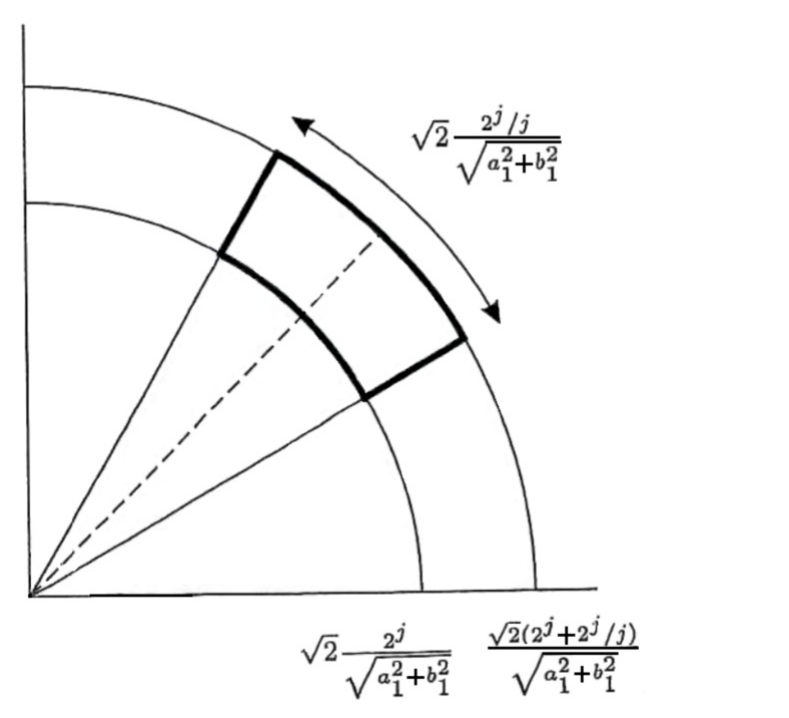
\includegraphics[width=0.36\textwidth]{figs/fig-8-riemann.png}
\end{center}

条件 $0 < |a_2/b_2 - 1| < 1/j$ 给出 $b_2 > j$，因此,
\begin{align*}
  \sqrt{2}\frac{2^{j}/j}{\sqrt{a_{1}^{2}+b_{1}^{2}}}\gtrsim 1,
\end{align*}
这使得该区域内的格点数可以用它的面积来估计. 于是
\begin{align*}
  \sum_{r_{j}(n)\geq 2}r_{j}^{2}(n)
  \lesssim\sum_{\substack{a_{1},b_{1}\\ 0<|a_{1}/b_{1}|<1/j}}\frac{4^{j}}{(a_{1}^{2}+b_{1}^{2})j^{2}}
  \lesssim\sum_{b_{1}<2^{j}}\frac{4^{j}}{b_{1}j^{3}}
  \lesssim\frac{4^{j}}{j^{2}},
\end{align*}
由此容易得出不等式 \eqref{eq:8.2}.
\end{proof}

\begin{proof}[引理~\ref{lem:8.5} 的证明]
首先观察（细节见 \cite{b24}）: 若 $n \equiv 0 \pmod 4$ 表为两平方和有两种不同的分解 $n = a^2 + b^2 = c^{2}+d^{2}$，则存在整数 $a_{1}, b_{1}, a_{2}$ 与 $b_{2}$，使
\begin{align*}
  n=\left(a_{1}^{2}+b_{1}^{2}\right)(a_{2}^{2}+b_{2}^{2}),
\end{align*}
\begin{align*}
  \frac{a_{1}}{b_{1}}=\tan\Big(\frac{\arctan(a/b)+\arctan(c/d)}{2}\Big),\qquad
  \frac{a_{2}}{b_{2}}=\tan\Big(\frac{\arctan(a/b)-\arctan(c/d)}{2}\Big).
\end{align*}
设 $n = a_r^2 + b_r^2 = a_s^2 + b_s^2$ 是 $n$ 表为两平方和的两种不同表示，满足
\begin{align*}
  2^{j}\leq a_{r}\leq b_{r}\leq 2^{j}+\frac{2^{j}}{j},\qquad
  2^{j}\leq a_{s}\leq b_{s}\leq 2^{j}+\frac{2^{j}}{j},
\end{align*}
\begin{align*}
  a_{r}\equiv b_{r}\equiv a_{s}\equiv b_{s}\equiv 0\pmod{2}.
\end{align*}
由前面的论证，存在 $a_{1}, b_{1}, a_{2}$ 与 $b_{2}$，使
\begin{align*}
  n=\left(a_{1}^{2}+b_{1}^{2}\right)(a_{2}^{2}+b_{2}^{2}),
\end{align*}
\begin{align*}
  \frac{a_{1}}{b_{1}}=\tan\Big(\frac{\arctan(a_{r}/b_{r})+\arctan(a_{s}/b_{s})}{2}\Big),
\end{align*}
\begin{align*}
  \frac{a_{2}}{b_{2}}=\tan\Big(\frac{\arctan(a_{r}/b_{r})-\arctan(a_{s}/b_{s})}{2}\Big).
\end{align*}
对 $a_{r}$，$b_{r}$，$a_{s}$ 与 $b_{s}$ 所加的条件容易给出
\begin{align*}
  \left|\frac{a_{2}}{b_{2}}\right|<\frac{1}{j},\qquad
  \left|\frac{a_{1}}{b_{1}}-1\right|<\frac{1}{j}.
\end{align*}
另一方面，两个量都严格大于 $0$，因为否则我们不可能从 $n$ 表为两平方和的两种不同表示出发.

每对不同表示
\begin{align*}
  \{n=a_{r}^{2}+b_{r}^{2}=a_{s}^{2}+b_{s}^{2},\ a_{s}\equiv b_{s}\equiv a_{r}\equiv b_{r}\equiv 0 \pmod 2\}
\end{align*}
产生不同的角，从而产生不同的整数 $a_1, b_1, a_2$ 与 $b_2$. 因此 $\binom{r_j(n)}{2}$ 以问题
\begin{align*}
  n=\left(a_{1}^{2}+b_{1}^{2}\right)\left(a_{2}^{2}+b_{2}^{2}\right),\qquad
  0<\left|\frac{a_{1}}{b_{1}}\right|<\frac{1}{j},\qquad
  0<\left|\frac{a_{2}}{b_{2}}-1\right|<\frac{1}{j}
\end{align*}
的解数为上界. 引理由观察 $r_j(n) \geq 2$ 时 $r_j^2(n) \leq 4\binom{r_j(n)}{2}$ 得出.
\end{proof}

\begin{remark}\label{rem:8.6}
不难看出，满足 $n_k^2 = o(k^2\log k)$ 的平方数子序列 $\{n_k^2\}$ 不可能具有性质 $B_2[\infty]$.

此外，可以构造增长非常快、却仍然不是 $B_2[\infty]$-序列的平方数序列.
\end{remark}

\section{平方频率的傅里叶级数}

关于频率为平方数的傅里叶级数的 $L^{p}$-特征的问题，在系数的单调性条件下有令人满意的答案.

\begin{proposition}\label{prop:8.7}
假设 $\{a_n\}$ 是非负实数的单调递减序列，且 $\sum_{n=0}^{\infty} a_n e^{2\pi i n^2x}$ 是可积函数 $f$ 的傅里叶级数. 则对每个 $p$，$1 \leq p < 4$，有 $f \in L^p[0,1]$，并满足估计
\begin{align*}
  \|f\|_{p}\lesssim\|f\|_{1}.
\end{align*}
\end{proposition}

上述命题的证明将基于下面的事实.

\begin{lemma}\label{lem:8.8}
设 $f$ 在 $[0, 1]$ 上连续，且满足
\begin{enumerate}
\item[(i)] $\|f\|_{\infty} \leq N$，$\|f\|_2 \leq N^{1/2}$；
\item[(ii)] 若 $|x - p/q| \leq 1/q^2$，则
\begin{align*}
  |f(x)|\leq C_{0}\left\{q^{1/k}+\frac{N}{q^{1/k}}\right\},\qquad \text{对某个常数 } C_{0}.
\end{align*}
\end{enumerate}
则 $f$ 满足 $2k$-弱型不等式
\begin{align*}
  \mu\{x:|f(x)|>\alpha>0\}\leq C\frac{N^{k}}{\alpha^{2k}}
\end{align*}
对每个 $\alpha > 0$ 成立，其中常数 $C = C(C_0)$ 与 $\alpha$ 和 $N$ 无关，$\mu$ 表示 $[0,1]$ 中的 Lebesgue 测度.
\end{lemma}

\begin{proof}
不失一般性，可以假设 $C_0 = 1$，因为若 $C_0 > 1$，只需考虑函数 $f/C_0$. 证明将等价于: 对每个 $\alpha > 0$,
\begin{align*}
  \mu(E_{\alpha})=\mu\{|f(x)|\geq 2N^{1/2}\alpha\}\leq\widetilde{C}\frac{1}{\alpha^{2k}},
\end{align*}
其中 $\widetilde{C}$ 与 $N$ 和 $\alpha$ 无关. 注意只须在 $\frac{1}{2}N^{1/2} \geq \alpha \geq 1$ 时证明，因为 $\alpha < 1$ 时不等式平凡化，而 $\alpha \geq \frac{1}{2}N^{1/2}$ 时 $E_{\alpha} = \emptyset$. 若
\begin{align*}
  x=\frac{1}{x_{1}+\frac{1}{x_{2}+\frac{1}{x_{3}+\cdots}}}
\end{align*}
是无理数 $x \in E_\alpha$ 的连分数展开，渐近分数为 $\{P_\nu/Q_\nu\}$，则下列成立:
\begin{align*}
  Q_{\nu}^{1/k}+\frac{N}{Q_{\nu}^{1/k}}\geq 2N^{1/2}\alpha.
\end{align*}
即，对每个 $\nu$,
\begin{align*}
  \text{或}\quad Q_{\nu}^{1/k}\geq N^{1/2}\alpha,\qquad
  \text{或}\quad N/Q_{\nu}^{1/k}\geq N^{1/2}\alpha.
\end{align*}
有两种可能的情形:

情形 1. $Q_1^{1/k} \geq N^{1/2}\alpha$，即 $Q_1 \geq N^{k/2}\alpha^k$.

由于 $x \leq 1/Q_1$，有 $x \in I_0 = [0, \frac{1}{N^{k/2}\alpha^k}]$，且
\begin{align*}
  \mu(I_{0})=\frac{1}{N^{k/2}\alpha^{k}}\leq\frac{1}{2^{k}\alpha^{2k}}.
\end{align*}

情形 2. 存在 $\nu \geq 1$，使
\begin{align*}
  \frac{N}{Q_{\nu}^{1/k}}\geq N^{1/2}\alpha,\qquad \text{即}\quad Q_{\nu}\leq\frac{N^{k/2}}{\alpha^{k}},
\end{align*}
以及
\begin{align*}
  Q_{\nu+1}^{1/k}\geq N^{1/2}\alpha,\qquad \text{即}\quad Q_{\nu+1}\geq N^{k/2}\alpha^{k}.
\end{align*}
有
\begin{align*}
  \left|x-\frac{P_{\nu}}{Q_{\nu}}\right|\leq\frac{1}{Q_{\nu}Q_{\nu+1}}
  \leq\frac{1}{Q_{\nu}}\frac{1}{N^{k/2}\alpha^{k}},
\end{align*}
即
\begin{align*}
  x\in\Bigl(\frac{P_{\nu}}{Q_{\nu}}-\frac{1}{Q_{\nu}}\frac{1}{N^{k/2}\alpha^{k}},
  \frac{P_{\nu}}{Q_{\nu}}+\frac{1}{Q_{\nu}}\frac{1}{N^{k/2}\alpha^{k}}\Bigr).
\end{align*}
给定满足 $r < s$，$\gcd(r, s) = 1$，$s \leq N^{k/2}/\alpha^k$ 的整数 $r$ 与 $s$，考虑区间
\begin{align*}
  I_{r,s}=\Bigl(\frac{r}{s}-\frac{1}{s}\frac{1}{N^{k/2}\alpha^{k}},
  \frac{r}{s}+\frac{1}{s}\frac{1}{N^{k/2}\alpha^{k}}\Bigr).
\end{align*}
则前面的观察给出包含关系
\begin{align*}
  E_{\alpha}\setminus\{\text{有理数}\}\subset I_{0}\bigcup\Big(\bigcup_{r,s}I_{r,s}\Big).
\end{align*}
因此,
\begin{align*}
  \mu(E_{\alpha})
  &\leq\mu(I_{0})+\sum_{\substack{r=1\\ (r,s)=1}}^{s-1}\sum_{s=1}^{N^{k/2}/\alpha^{k}}\mu(I_{r,s})
  \leq\frac{1}{\alpha^{2k}}+\sum_{s=1}^{N^{k/2}/\alpha^{k}}\sum_{r=1}^{s-1}
   \frac{2}{s}\frac{1}{N^{k/2}\alpha^{k}}\\
  &\leq\frac{1}{\alpha^{2k}}+\sum_{s=1}^{N^{k/2}/\alpha^{k}}\frac{2}{N^{k/2}\alpha^{k}}
  \leq\frac{3}{\alpha^{2k}}.
\end{align*}
\end{proof}

接下来考虑三角多项式
\begin{align*}
  S_{N}(x;y)=\sum_{n=1}^{N}e^{2\pi i(n^{2}x+ny)}
\end{align*}
及其 Carleson 极大函数
\begin{align*}
  C_{N}^{*}(x;y)=\sup_{1\leq M\leq N}|S_{M}(x;y)|.
\end{align*}
现在用 Carleson 极大定理继续命题 8.7 的证明，证明对每个 $y \in [0,1]$，$S_N(x; y)$ 在 $k = 2$ 的情形满足引理 8.8 的假设.

\begin{lemma}\label{lem:8.9}
设 $x$ 有形如 $|x - p/q| \leq 1/q^2$ 的有理逼近，$1 \leq q \leq N^2$，$\gcd(p, q) = 1$. 则
\begin{align*}
  C_{N}^{*}(x;y)\lesssim\left\{q^{1/2}+\frac{N}{q^{1/2}}\right\}.
\end{align*}
\end{lemma}

这个结果 Hardy 与 Littlewood \cite{b187,b188} 已知，他们用 $\theta$-函数的近似函数方程证明了它. 下面 E.~Bombieri 的证明，见 \cite{b173}，通过使用 Carleson 定理 \cite{b175} 强调了数论与调和分析之间的联系.

\begin{proof}
首先注意，若 $|x - x_0| \leq \frac{1}{4N^2}$ 且 $|y - y_0| \leq \frac{1}{4N}$，则有不等式
\begin{align*}
  C_{N}^{*}(x;y)\leq 100C_{N}^{*}(x_{0};y_{0}).
\end{align*}
这是因为
\begin{align*}
  S_{M}(x;y)
  &=\sum_{n=1}^{M}e^{2\pi i(n^{2}x+ny)}
  =\sum_{n=1}^{M}e^{2\pi i(n^{2}x_{0}+ny_{0})}\cdot e^{2\pi i(n^{2}(x-x_{0})+n(y-y_{0}))}\\
  &=\sum_{n=1}^{M}\left(S_{n}(x_{0};y_{0})-S_{n-1}(x_{0};y_{0})\right)e^{2\pi i(n^{2}(x-x_{0})+n(y-y_{0}))}\\
  &=\sum_{n=1}^{M-1}S_{n}(x_{0};y_{0})\left(e^{2\pi i(n^{2}(x-x_{0})+n(y-y_{0}))}
   -e^{2\pi i((n+1)^{2}(x-x_{0})+(n+1)(y-y_{0}))}\right)\\
  &\quad+S_{M}(x_{0};y_{0})e^{2\pi i(M^{2}(x-x_{0})+M(y-y_{0}))}.
\end{align*}
对 $M$，$1 \leq M \leq N$，取上确界，得
\begin{align*}
  C_{N}^{*}(x;y)
  &\leq 2C_{N}^{*}(x_{0};y_{0})\left[1+\sum_{n=1}^{N}(|x-x_{0}|4\pi n+4\pi|y-y_{0}|)\right]\\
  &\leq 100C_{N}^{*}(x_{0};y_{0}).
\end{align*}
其次，对所有 $M$，$1 \leq M \leq N$，有下列不等式:
\begin{align*}
  C_{N}^{*}(x;y)\leq 2C_{2N}^{*}(x;y-2Mx),
\end{align*}
因为对所有 $K \leq N$,
\begin{align*}
  \left|S_{K}(x;y)\right|
  &=\Big|\sum_{n=1}^{K}e^{2\pi i(n^{2}x+ny)}\Big|
  =\Big|\sum_{n=M+1}^{K+M}e^{2\pi i((n-M)^{2}x+(n-M)y)}\Big|\\
  &=\Big|\sum_{n=M+1}^{K+M}e^{2\pi i(n^{2}x+n(y-2Mx))}\Big|
  \leq 2C_{2N}^{*}(x;y-2Mx).
\end{align*}
把不等式平方并对 $M$ 取平均，得
\begin{align*}
  |C_{N}^{*}(x;y)|^{2}
  &\leq\frac{4}{N}\sum_{M=1}^{N}|C_{2N}^{*}(x;y-2Mx)|^{2}\\
  &\leq\frac{4}{N}\sum_{n=1}^{M}(100)^{2}8N\int_{I(2Mx-y)}|C_{2N}^{*}(x;y_{0})|^{2}\,\mathrm{d}y_{0},
\end{align*}
其中 $I(z) = \{w : |z - w| \leq \frac{1}{8N}\}$. 初等计算给出区间族 $\{I_{(2M x - y)}\}$ 重叠的上界:
\begin{align*}
  \Big\|\sum_{M=1}^{N}\chi_{I_{(2M x-y)}}\Big\|_{\infty}\lesssim\Big(\frac{N}{q}+\frac{q}{N}\Big),
\end{align*}
应用 Carleson 极大定理，得
\begin{align*}
  C_{N}^{*}(x;y)^{2}\lesssim\left\{q+\frac{N^{2}}{q}\right\}.
\end{align*}
\end{proof}

\begin{proof}[命题~\ref{prop:8.7} 的证明]
考虑极大函数
\begin{align*}
  C_{N}^{*}(x)=\sup_{1\leq M\leq N}\Big|\sum_{n=1}^{M}e^{2\pi i n^{2}x}\Big|.
\end{align*}
则引理 8.8 与 8.9 给出估计
\begin{align*}
  \mu(\{C_{N}^{*}(x)\geq 2N^{1/2}\alpha\})\lesssim\frac{1}{\alpha^{4}},
\end{align*}
特别地，得到
\begin{align*}
  \|C_{N}^{*}\|_{p}\leq C_{p}N^{1/2},\qquad 2\leq p<4.
\end{align*}
给定傅里叶级数 $f = \sum a_n e^{2\pi i n^2 x}$，有 Littlewood--Paley 范数等价
\begin{align*}
  \|f\|_{p}\simeq\Big\|\Big(\sum_{k}|\Delta_{k}(x)|^{2}\Big)^{1/2}\Big\|_{p},\qquad 1<p<\infty,
\end{align*}
其中
\begin{align*}
  \Delta_{k}(x)=\sum_{n=2^{k}}^{2^{k+1}-1}a_{n} e^{2\pi i n^{2}x}.
\end{align*}
特别地，对 $2 \leq p < 4$ 有
\begin{align*}
  \|f\|_{p}
  &\lesssim\Big[\int_{0}^{1}\Big(\sum_{k}|\Delta_{k}(x)|^{2}\Big)^{p/2}\Big]^{\frac{2}{p}\cdot\frac{1}{2}}
  \leq\Big[\sum_{k}\Big(\int_{0}^{1}|\Delta_{k}|^{p}\Big)^{2/p}\Big]^{1/2}\\
  &=\Big(\sum_{k}\|\Delta_{k}\|_{p}^{2}\Big)^{1/2}.
\end{align*}
但
\begin{align*}
  \Delta_{k}(x)
  &=\sum_{n=2^{k}}^{2^{k+1}-1}a_{n} e^{2\pi i n^{2}x}
  =\sum_{n=2^{k}}^{2^{k+1}-1}a_{n}\left[S_{n}(x)-S_{n-1}(x)\right]\\
  &=\sum_{n=2^{k}}^{2^{k+1}-1}(a_{n}-a_{n+1})S_{n}(x)+a_{2^{k+1}-1}S_{2^{k+1}-1}(x),
\end{align*}
其中 $S_{n}(x)$ 表示 $f$ 的部分和. 由于系数单调递减，得
\begin{align*}
  \left|\Delta_{k}(x)\right|\leq 2C_{2^{k+1}}^{*}(x)\cdot a_{2^{k}}.
\end{align*}
因此,
\begin{align*}
  \|f\|_{p}\lesssim\Big(\sum_{k}a_{2^{k}}^{2}\cdot 2^{k}\Big)^{1/2}\lesssim\|f\|_{2}.
\end{align*}
\end{proof}

\section{Riemann 图象的分形维数}

在他的学位论文中，Riemann 还引入了几类在一个稠密点集上不可微的连续函数；这一纲领由 Weierstrass 完成，他用缺项三角级数构造了第一个已知的连续而处处不可微的函数. 似乎 Weierstrass 受到了归功于 Riemann 的错误断言的启发: 下面两个连续函数
\begin{align*}
  F(x)=\sum_{n=1}^{\infty}\frac{\sin(2\pi n^{2}x)}{n^{2}},\qquad
  G(x)=\sum_{n=1}^{\infty}\frac{\cos(2\pi n^{2}x)}{n^{2}}
\end{align*}
处处不可微.

这些函数已被若干作者研究，如今我们对它们的可微点有相当完整的认识. 下面，我们将关心它们图象的 Minkowski（计盒）维数.

\begin{remark}\label{rem:8.10}
给定小数 $h = N^{-1}$，单位区间 $[0,1)$ 可以分解为子区间 $I_j = [(j-1)h, jh)$，$j = 1,2,\ldots,N$ 的不交并. 覆盖连续函数 $F\colon [0,1) \to \R$ 的图象所需的边长为 $h$ 的盒子数是
\begin{align*}
  A_{h}=\sum_{j=1}^{N}\sup_{x,y\in I_{j}}|F(x)-F(y)|+o(h^{-1}).
\end{align*}
由此容易得出，$F$ 图象的\newterm{fractal-dimension}{分形维数}{fractal dimension}（计盒维数，或 Minkowski 维数）由下面的极限给出:
\begin{align*}
  \dim(\mathrm{graph}(F))=-\lim_{h\to 0^{+}}\frac{\log A_{h}}{\log h}.
\end{align*}
如（第 3 章）已指出的，上述量只在极限存在时才有意义. 因此，方便的做法是定义下、上分形维数 $\underline{\dim}$ 与 $\overline{\dim}$，分别以 $\underline{\lim} = \liminf$ 与 $\overline{\lim} = \limsup$ 代替 $\lim$.
\end{remark}

给定 $0 < \delta \leq 1$，考虑连续函数族
\begin{align*}
  F_{\delta}(x)=\sum_{n=1}^{\infty}\frac{\sin(2\pi n^{2}x)}{n^{1+\delta}},\qquad
  G_{\delta}(x)=\sum_{n=1}^{\infty}\frac{\cos(2\pi n^{2}x)}{n^{1+\delta}}.
\end{align*}

\begin{theorem}[{[\cite{b176}]}]\label{thm:8.11}
$\dim_{\mathrm{B}}(\operatorname{graph}(F_{\delta})) = \dim_{\mathrm{B}}(\operatorname{graph}(G_{\delta})) = 7/4 - \delta/2$.
\end{theorem}

\begin{proof}
固定（大的）整数 $N$，设 $J_{a/q}$ 是 $N^{1/2}$ 阶 Farey 剖分中 $a/q$ 所在的弧，即
\begin{align*}
  (0,1]=\bigcup_{a,q}J_{a/q},\qquad
  J_{a/q}=\Big(\frac{a^{\prime}+a}{q^{\prime}+q},\frac{a+a^{\prime\prime}}{q+q^{\prime\prime}}\Big),
\end{align*}
其中 $a'/q' < a/q < a''/q''$ 是 Farey 序列 $F_{N^{1/2}}$ 中三个相邻的分数.

有
\begin{align*}
  J_{a/q}\subset\left\{x\in(0,1]:\left|x-\frac{a}{q}\right|<\frac{1}{q N^{1/2}}\right\}.
\end{align*}
其次，考虑不完全高斯和
\begin{align*}
  S_{n,m}(x)=\sum_{k=m+1}^{n}e^{2\pi i k^{2}x},\qquad
  S_{n}(x)=S_{n,0}(x).
\end{align*}
从前一节，我们知道估计
\begin{align*}
  |S_{n,m}(x)|\lesssim\frac{n}{\sqrt{q}}+\sqrt{q},
\end{align*}

\begin{figure}[htbp]
\centering
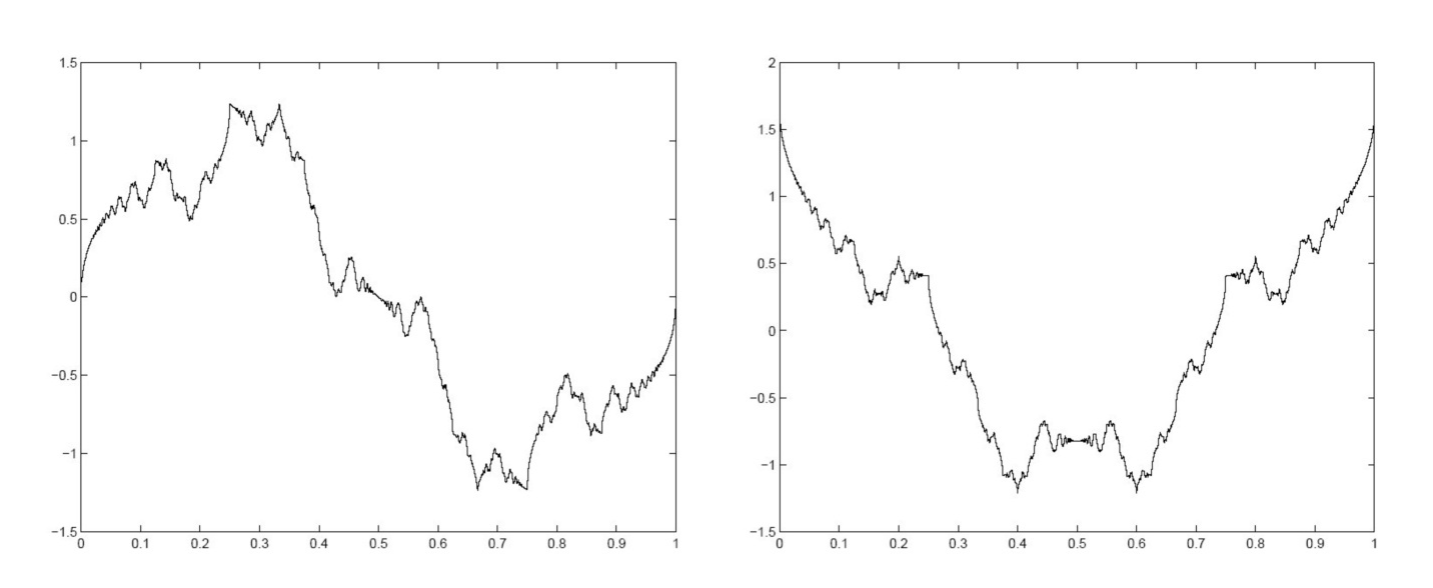
\includegraphics[width=0.7\textwidth]{figs/fig-8-1.png}
\caption{$F_{1}(x)$（左）与 $G_{1}(x)$（右）的图象.}
\label{fig:8.1}
\end{figure}

\begin{figure}[htbp]
\centering
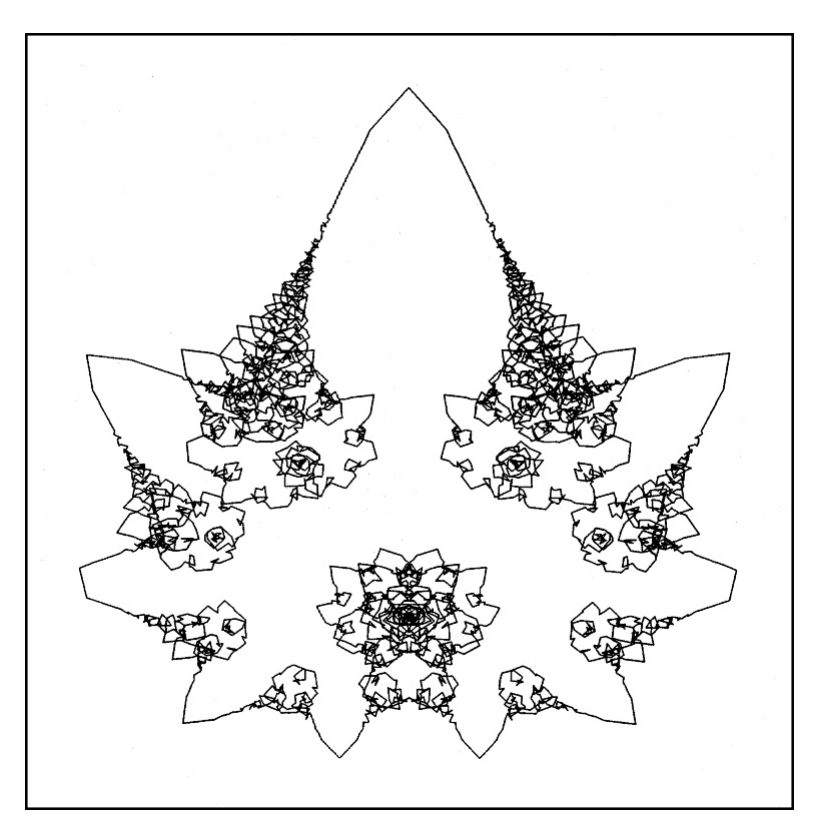
\includegraphics[width=0.42\textwidth]{figs/fig-8-2.png}
\caption{$\sigma(t) = (F_{1/2}(t), G_{1/2}(t))$ 的图象.}
\label{fig:8.2}
\end{figure}

只要 $|x - a/q| \leq 1/q^2$. 对完全和，有显式求值
\begin{align*}
  \sum_{k=1}^{q}e^{2\pi i\frac{a}{q}k^{2}}=\varepsilon_{q}\sqrt{q}\left(\frac{a}{q}\right),\qquad \text{若 } \gcd(a,q)=1,
\end{align*}
其中 $\left(\frac{a}{q}\right)$ 表示 Legendre 符号，而
\begin{align*}
  \varepsilon_{q}=\begin{cases}
    1, & \text{若 } q\equiv 1\pmod 4,\\
    i, & \text{若 } q\equiv 3\pmod 4,\\
    0, & \text{若 } q\equiv 2\pmod 4,\\
    1+i, & \text{若 } q\equiv 0\pmod 4.
  \end{cases}
\end{align*}
给定 $n' = m + q\left[\frac{n-m}{q}\right]$，有
\begin{align*}
  S_{n,m}(a/q)=S_{n'-1,m}(a/q)+S_{n,n'}(a/q)
  =\varepsilon_{q}\left(\frac{a}{q}\right)\frac{n-m}{\sqrt{q}}+O(\sqrt{q}).
\end{align*}
设 $\alpha(a/q; N)$ 是覆盖交集 $\mathrm{graph}(F_\delta) \cap (J_{a/q} \times \R)$ 所需的网格
\begin{align*}
  \mathcal{M}_{N}=\left\{x=\frac{\ell}{N},y=\frac{m}{N};0\leq\ell\leq N\right\}
\end{align*}
的盒子数，设 $\alpha(a/q; N, k)$ 是其中包含于带形 $I_k \times \R$（$I_k = [k/N, (k+1)/N]$）内的盒子数.

(i) 首先证明上界
\begin{align*}
  \overline{\dim}_{\mathrm{B}}(\mathrm{graph}(F_{\delta}))\leq\frac{7}{4}-\frac{\delta}{2}.
\end{align*}
设 $M$ 是待定的正整数. 由 $\alpha(a/q; N, k)$ 的定义，应用均值定理后得
\begin{align*}
  \alpha\Big(\frac{a}{q};N,k\Big)
  &\leq 2+N\sup_{x,y\in I_{k}\cap J_{a/q}}|F_{\delta}(x)-F_{\delta}(y)|\\
  &\leq 2+4\pi\Big|\sum_{n\leq M}n^{1-\delta}e^{2\pi i n^{2}\xi}\Big|
   +N\Big|\sum_{n\geq M}\frac{1}{n^{1+\delta}}\left(e^{2\pi i n^{2}x_{0}}-e^{2\pi i n^{2}y_{0}}\right)\Big|,
\end{align*}
其中 $\xi, x_0, y_0 \in I_k \cap J_{a/q}$. 分部求和给出
\begin{align*}
  \alpha\Big(\frac{a}{q};N,k\Big)
  &\lesssim 4\pi\Big|\sum_{n\leq M}\left[n^{1-\delta}-\left(n+1\right)^{1-\delta}\right]S_{n}(\xi)\Big|\\
  &\quad+\left|S_{M}(\xi)\right|M^{1-\delta}
   +\left(1+\delta\right)N\sum_{n>M}\frac{\left|S_{n,M}(x_{0})\right|+\left|S_{n,M}(y_{0})\right|}{n^{2+\delta}}.
\end{align*}
现在选取 $M = [\sqrt{N}]$，由高斯和的已知估计，得
\begin{align*}
  \alpha\Big(\frac{a}{q};N,k\Big)
  &\lesssim\Big(\frac{M}{\sqrt{q}}+\sqrt{q}\Big)+\Big(\frac{M}{\sqrt{q}}+\sqrt{q}\Big)M^{1-\delta}
   +N\Big[\frac{1}{q^{1/2}}\cdot\frac{1}{N^{\frac{1}{2}(\frac{1}{2}+\delta)}}\Big]\\
  &\lesssim N^{1-\delta/2}\frac{1}{\sqrt{q}}+N^{1/2-\delta/2}\sqrt{q}.
\end{align*}
其次注意
\begin{align*}
  \alpha\Big(\frac{a}{q};N\Big)
  \lesssim\frac{|J_{a/q}|}{1/N}\Big(N^{1-\delta/2}\frac{1}{\sqrt{q}}+N^{1-\delta/2}\sqrt{q}\Big)
  \lesssim\frac{N^{3/2-\delta/2}}{q^{3/2}}+N^{1-\delta/2}\frac{1}{q^{1/2}}.
\end{align*}
于是，覆盖图象所需的网格 $\mathcal{M}_N$ 盒子数以
\begin{align*}
  \sum_{q\leq N^{1/2}}\sum_{(a,q)=1}\left(\frac{N^{3/2-\delta/2}}{q^{3/2}}+N^{1-\delta/2}\frac{1}{q^{1/2}}\right)
  &\lesssim\sum_{q\leq N^{1/2}}\left(\frac{N^{3/2-\delta/2}}{q^{1/2}}+N^{1-\delta/2}q^{1/2}\right)\\
  &\lesssim N^{7/4-\delta/2}
\end{align*}
为界，由此得上界
\begin{align*}
  \overline{\dim}_{\mathrm{B}}(\mathrm{graph}(F_{\delta}))
  \leq\limsup_{N\to\infty}\frac{\log(N^{7/4-\delta/2})}{\log N}
  =\frac{7}{4}-\frac{\delta}{2}.
\end{align*}
显然，同样的证明也表明
\begin{align*}
  \overline{\dim}_{\mathrm{B}}(\operatorname{graph}(G_{\delta}))\leq\frac{7}{4}-\frac{\delta}{2}.
\end{align*}

(ii) 现在证明下界
\begin{align*}
  \underline{\dim}_{\mathrm{B}}(\operatorname{graph}(F_{\delta}))\geq\frac{7}{4}-\frac{\delta}{2},\qquad
  \underline{\dim}_{\mathrm{B}}(\operatorname{graph}(G_{\delta}))\geq\frac{7}{4}-\frac{\delta}{2}.
\end{align*}
这里需要分开两种情形. 对 $F_{\delta}$，选取 $P$ 为满足 $p \equiv 3 \pmod 4$ 且 $p \asymp \sqrt{N}$ 的素数集. 对 $G_{\delta}$，类似进行，但（出于显然的原因）换成素数 $p \equiv 1 \pmod 4$.

由 Minkowski 维数的定义，有
\begin{align*}
  \underline{\dim}_{\mathrm{B}}(\operatorname{graph}(F_{\delta}))
  \geq\liminf_{N\to\infty}\frac{\log\bigl(N\sum_{p\in P}\sum_{0\leq a\leq p}|F_{\delta}(a/p)-F_{\delta}(a/p+1/p^{2})|\bigr)}{\log N}.
\end{align*}
接着，只考虑模 $p$ 的二次剩余所组成的集合 $\mathcal{R}(p)$ 中的 $a$ 值. 这些 $a$ 的相应和大于
\begin{align*}
  \sum_{a\in\mathcal{R}(p)}\Big(F_{\delta}\Big(\frac{a}{p}\Big)-F_{\delta}\Big(\frac{a}{p}+\frac{1}{p^{2}}\Big)\Big)
  &=\operatorname{Im}\Big(\sum_{n}\sum_{r=1}^{(p-1)/2}\frac{e^{2\pi i r^{2}n^{2}/p^{2}}}{n^{1+\delta}}
   \left(1-e^{2\pi i n^{2}/p^{2}}\right)\Big)\\
  &=\operatorname{Im}\Big(\sum_{n}\frac{(-1+i\sqrt{p})\left(1-e^{2\pi i n^{2}/p^{2}}\right)}{2n^{1+\delta}}\Big)\\
  &=\sqrt{p}\sum_{n}\frac{\sin^{2}(\pi n^{2}/p^{2})}{n^{1+\delta}}
   +\sum_{n}\frac{\sin(2\pi n^{2}/p^{2})}{2n^{1+\delta}}
  \gtrsim p^{1/2-\delta}
\end{align*}
的绝对值. 算术级数中的素数定理给出
\begin{align*}
  \underline{\dim}_{\mathrm{B}}(\operatorname{graph}(F_{\delta}))
  \geq\lim_{N\to\infty}\frac{\log\left(N\cdot N^{1/4-\delta/2}\cdot N^{1/2}/\log N^{1/2}\right)}{\log N}
  =\frac{7}{4}-\frac{\delta}{2}.
\end{align*}
\end{proof}

定理 8.11 向高于二次的幂的推广需要数论的若干结果.

解析数论中许多有趣命题的证明，有时可以化归为得到指数和的非平凡上界. 估计这类和的第一种方法由 Weyl 于 1916 年创立，它完全基于下面的引理（见 \cite{b196}）.

\begin{lemma}[Weyl 不等式]\label{lem:8.12}
若 $P$ 是 $k$ 次多项式，$a/q$ 是不可约分数，且多项式 $P$ 的首项系数 $A$ 满足 $|A - a/q| \leq q^{-2}$，则
\begin{align*}
  \sum_{n\leq N}e\left(P(n)\right)
  \lesssim\left(N q^{-1/K}+N^{1-1/K}+N^{1-k/K}q^{1/K}\right)N^{\varepsilon}
\end{align*}
对 $K = 2^{k-1}$ 与每个 $\varepsilon > 0$ 成立.
\end{lemma}

用归功于 I.~M.~Vinogradov 的方法，可以对大的 $k$ 改进 Weyl 不等式. Vinogradov 方法可以得到若干类结果，下面这个取自 \cite{b184} 的 Th\'eor\`eme 10.1（对陈述略作简化）.

\begin{lemma}\label{lem:8.13}
设 $P, k, A$ 与 $q$ 如 Weyl 不等式. 则对 $k \geq 9$ 与 $N \leq q \leq N^{k-2}$，有估计
\begin{align*}
  \sum_{n\leq N}e(P(n))\lesssim N^{1-\delta},
\end{align*}
其中 $\delta = (9k^2\log k)^{-1}$.
\end{lemma}

在某些语境中（例如研究素数之和时），指数和出现时带有只能被平均地控制的系数，因而分部求和不适用. 大筛不等式允许在某些情形下，若这类指数和的个数足够多，则获得相消. 大筛不等式依语境有若干表述；也许最简单的如下（见 \cite{b172}）.

\begin{lemma}[大筛不等式]\label{lem:8.14}
设 $\delta > 0$，$\{t_\nu\}_{\nu=1}^R$ 满足 $0 \leq t_1 < t_2 < \cdots < t_R < 1 - \delta$，且 $t_{\nu+1} - t_\nu > \delta$. 则
\begin{align*}
  \sum_{\nu=1}^{R}\Big|\sum_{n\leq N}a_{n} e\left(n t_{\nu}\right)\Big|^{2}
  \leq\left(N+\delta^{-1}\right)\sum_{n\leq N}|a_{n}|^{2}
\end{align*}
对任意复数 $a_{n}$ 成立.
\end{lemma}

现在考虑函数族
\begin{align*}
  F_{\alpha,k}(x)=\sum_{n=1}^{\infty}\frac{c_{n} e(n^{k} x)}{n^{\alpha}},\qquad
  0<\varliminf c_{n}\leq\varlimsup c_{n}<\infty.
\end{align*}
可以计算它们图象的分形维数.

\begin{theorem}\label{thm:8.15}
若 $(k+1)/2 \leq \alpha \leq k+1/2$，则
\begin{align*}
  \dim(F_{\alpha,k})=2+\frac{1}{2k}-\frac{\alpha}{k}.
\end{align*}
\end{theorem}

\begin{remark}\label{rem:8.16}
注意这一结果蕴含: 对 $(k+1)/2 \leq \alpha < k+1/2$，$F_{\alpha,k}$ 的分形维数是非整数. 另一方面，若 $\alpha > k+1/2$，则 $F_{\alpha,k}$ 绝对连续（注意 $F_{\alpha,k}' \in L^2$），分形维数平凡地等于一. 在猜想界 $\|\sum_{n \leq N} c_n e(n^k x)\|_{2k} = O(N^{1/2+\varepsilon})$（对 $k = 2$ 成立）之下，范围可以补全到 $1 < \alpha \leq k+1/2$.
\end{remark}

\begin{proof}[定理~\ref{thm:8.15} 的证明]
首先证明上界
\begin{equation}\label{eq:8.3}
  \overline{\dim}(F_{\alpha,k})\leq 2+\frac{1}{2k}-\frac{\alpha}{k}.
\end{equation}
给定 $x, y \in I$，其中 $I$ 是长度为 $h$ 的闭区间，把 $F_{\alpha, k}$ 的项按 $n > h^{-1/(k-1)}$ 分开，并对 $n \leq h^{-1/k}$ 的项应用均值定理. 则得到
\begin{align*}
  |F_{\alpha,k}(x)-F_{\alpha,k}(y)|
  \lesssim h\left|S_{1}(\xi)\right|+|S_{2}(x)|+|S_{2}(y)|+h^{(\alpha-1)/(k-1)},
\end{align*}
其中
\begin{align*}
  S_{1}(\xi)=\sum_{n\leq h^{-1/k}}c_{n}n^{k-\alpha}e(n^{k}\xi),\qquad
  S_{2}(t)=\sum_{h^{-1/k}<n\leq h^{-1/(k-1)}}\frac{c_{n}e(n^{k}t)}{n^{\alpha}},
\end{align*}
$\xi \in I$. 取 $I = I_j$（$I_j$ 如分形维数定义中），并分离 $j$ 为奇、偶时对 $A_h$（定义于注 8.10）的贡献，有
\begin{equation}\label{eq:8.4}
  A_{h}\lesssim\sum_{\nu}\left|S_{1}(t_{\nu})\right|
  +h^{-1}\sum_{\nu}\left|S_{2}(t_{\nu}^{\prime})\right|
  +h^{(\alpha-2k+1)/(k-1)},
\end{equation}
其中 $h < t_{\nu+1} - t_{\nu}$，$t_{\nu+1}^{\prime} - t_{\nu}^{\prime} < 3h$.

把 $S_{2}$ 细分成二进区间，得
\begin{align*}
  S_{2}(t_{\nu}^{\prime})\lesssim\sum_{M}\Big|\sum_{M<n\leq 2M}\frac{c_{n}e(n^{k}t_{\nu}^{\prime})}{n^{\alpha}}\Big|,
\end{align*}
其中 $M = 2^m h^{-1/k}$，$h^{-1/k} \leq M < h^{-1/(k-1)}$. 再把每个二进区间 $(M, 2M]$ 细分为长度 $h^{-1}M^{1-k}$ 的区间，对每个 $M$ 找到 $M_1$ 与 $M_2$，使 $M < M_1 < M_2 \leq 2M$，$M_2 < M_1 + h^{-1}M^{1-k}$，且
\begin{align*}
  \sum_{\nu}|S_{2}(t_{\nu}^{\prime})|
  \lesssim\sum_{M}\frac{M}{h^{-1}M^{1-k}}\sum_{\nu}
  \Big|\sum_{M_{1}<n\leq M_{2}}\frac{c_{n}e(n^{k}t_{\nu}^{\prime})}{n^{\alpha}}\Big|.
\end{align*}
记最内层的和为 $S_{2M}(t'_\nu)$. 则由 \eqref{eq:8.4} 与 Cauchy 不等式，得
\begin{equation}\label{eq:8.5}
  A_{h}^{2}\lesssim h^{-1}\sum_{\nu}|S_{1}(t_{\nu})|^{2}
  +h^{-1}\sum_{M}M^{2k+\varepsilon}\sum_{\nu}|S_{2M}(t_{\nu}^{\prime})|^{2}
  +h^{(2\alpha-4k+2)/(k-1)}.
\end{equation}
大筛不等式蕴含
\begin{align*}
  \sum_{\nu}|S_{1}(t_{\nu})|^{2}
  \lesssim(h^{-1}+h^{-1})\sum_{n\leq h^{-1/k}}|c_{n}|^{2}n^{2k-2\alpha}
  \lesssim h^{-3+(2\alpha-1)/k-\varepsilon},
\end{align*}
以及
\begin{align*}
  \sum_{\nu}|S_{2M}(t_{\nu}^{\prime})|^{2}
  \lesssim(h^{-1}+h^{-1})\sum_{M_{1}<n<M_{2}}|c_{n}|^{2}M^{-2\alpha}
  \lesssim h^{-2}M^{1-k-2\alpha}.
\end{align*}
因此，代入 \eqref{eq:8.5},
\begin{align*}
  A_{h}^{2}\lesssim h^{-4+(2\alpha-1)/k-\varepsilon},
\end{align*}
由此得 \eqref{eq:8.3}.

现在证明下界
\begin{equation}\label{eq:8.6}
  \underline{\dim}(F_{\alpha,k})\geq 2+\frac{1}{2k}-\frac{\alpha}{k}.
\end{equation}
设
\begin{align*}
  f(x)=F_{\alpha,k}(x+h)-F_{\alpha,k}(x).
\end{align*}
由 $A_{h}$ 的定义与 Hölder 不等式,
\begin{equation}\label{eq:8.7}
  A_{h}\geq h^{-2}\|f\|_{1}\geq h^{-2}\frac{\|f\|_{2}^{3}}{\|f\|_{4}^{2}}.
\end{equation}
Parseval 恒等式证明
\begin{align*}
  \|f\|_{2}^{2}=\sum_{n}|c_{n}|^{2}\frac{|1-e(n^{k}h)|^{2}}{n^{2\alpha}}.
\end{align*}
只考虑 $1/(4h) < n^{k} < 3/(4h)$ 的贡献，得到
\begin{align*}
  \|f\|_{2}^{2}\gtrsim h^{(2\alpha-1)/k}.
\end{align*}
另一方面，细分成二进区间后，对每个 $\varepsilon > 0$ 有
\begin{align*}
  \|f\|_{4}^{4}\lesssim\sup_{N}N^{\varepsilon}
  \Big\|\sum_{N\leq n<2N}c_{n}\frac{1-e(n^{k}h)}{n^{\alpha}}e(n^{k}x)\Big\|_{4}^{4},
\end{align*}
从而再次用 Parseval 恒等式,
\begin{align*}
  \|f\|_{4}^{4}\lesssim\sup_{N}N^{\varepsilon-4\alpha}
  \sum_{N\leq n<2N}\sum_{N\leq m<2N}
  |r_{k}\left(n^{k}+m^{k}\right)|^{2}|c_{n}|^{2}|c_{m}|^{2}
  |1-e(n^{k}h)|^{2}|1-e(m^{k}h)|^{2},
\end{align*}
其中 $r_k$ 表示表为两个 $k$ 次幂之和的表法个数. 有 $r_k(l) \lesssim l^{\varepsilon}$（因为 $l = m^k + n^k$ 蕴含: 若 $k$ 为奇，$m + n$ 整除 $l$；若 $k$ 为偶，$m^{k/2} + in^{k/2}$ 在 $\Z[i]$ 中整除 $l$；而因子个数增长得比任何正幂都慢）. 则
\begin{align*}
  \|f\|_{4}^{4}
  &\lesssim\sup_{N}N^{\varepsilon-4\alpha}
   \Big(\sum_{N\leq n<2N}|c_{n}|^{2}|1-e(n^{k}h)|^{2}\Big)^{2}\\
  &\lesssim\sup_{N}N^{\varepsilon-4\alpha}\min\left(N^{2},N^{2+2k}h^{-2}\right)
  \lesssim h^{(4\alpha-2)/k-\varepsilon}.
\end{align*}
把 $\|f\|_2$ 与 $\|f\|_4$ 的界代入 \eqref{eq:8.7}，得出
\begin{align*}
  A_{h}\gtrsim h^{-2-1/2k+\alpha/k+\varepsilon}
\end{align*}
对每个 $\varepsilon > 0$ 成立，这蕴含 \eqref{eq:8.6}.
\end{proof}

\section{晶体学部分和的收敛与发散}

取函数 $f \in L^{1}(\T)$，考虑其傅里叶级数
\begin{align*}
  \sum_{k=-\infty}^{\infty}\widehat{f}(k)e^{2\pi i k x},
\end{align*}
其中 $\widehat{f}(k)=\int_{0}^{1}f(x)e^{-2\pi i k x}\,\mathrm{d}x$. 这里 $\T$ 以通常方式等同于 $[0, 1)$. 通过傅里叶系数 $(\widehat{f}(k))_{k \in \Z}$ 重建函数 $f$ 的传统方式是考虑 $N$-部分和
\begin{equation}\label{eq:8.8}
  S_{N}f(x)=\sum_{|k|\leq N}\widehat{f}(k)\,e^{2\pi i k x}.
\end{equation}
众所周知有范数收敛: 若 $f \in L^p(\T)$，$1 < p < \infty$，则当 $N\to\infty$ 时
\begin{align*}
  S_{N}f\to f\quad\text{于 } L^{p}(\T).
\end{align*}
而自 Carleson \cite{b175}（其后 Hunt \cite{b191}）以来，还知道有几乎处处收敛.

然而，考虑到把傅里叶系数解释为周期分布的衍射图样，似乎更自然的做法是关注那些给我们更多信息的系数，即模更大的系数，并按傅里叶系数的模递减顺序重建函数. 即，对每个 $\lambda > 0$ 考虑部分和
\begin{equation}\label{eq:8.9}
  \tilde{S}_{\lambda}f(x)=\sum_{|\widehat{f}(k)|>\lambda}\widehat{f}(k)e^{2\pi i k x},
\end{equation}
以及它们在 $\lambda \to 0$ 时的极限.

1996 年，见 \cite{b192}，T.~W.~Körner 否定了 L.~Carleson 与 R.~Coifman 提出的一个问题，证明了存在函数 $f \in L^2(\T)$，使
\begin{equation}\label{eq:10}
  \limsup_{\lambda\to 0^{+}}\Big|\sum_{|\widehat{f}(k)|\geq\lambda}\widehat{f}(k)e^{2\pi i k x}\Big|=\infty
  \quad\text{对几乎每个 } x\in\T.
\end{equation}
当按递减系数求和时傅里叶级数的这种``坏''行为，例如与其他基（如小波）的情形形成对照，见 \cite{b195}.

Körner 的证明基于对归功于 Olevskii 的构造的巧妙修改，还用到 R.~Salem 与 A.~Zygmund 的一个概率引理. 具有所需性质的函数没有显式构造.

\section*{一个用高斯和的构造}

利用高斯和，可以产生满足 \eqref{eq:10} 的函数 $f \in L^p(\T)$（$p < 4/3$）的显式例子. 注意这个 $p$ 的范围，并与 Körner 的结果比较.

构造如下. 固定 $\varepsilon > 0$. 对每个 $k \geq 0$，取
\begin{equation}\label{eq:11}
  f_{k}(x)=\sum_{n=2^{2k}}^{2^{2k+2}-1}a_{n}\cos(2\pi n x),
\end{equation}
其中
\begin{align*}
  a_{n}=\begin{cases}
    \frac{1}{2^{k/2-k\varepsilon}}\left(1+\frac{1}{n}\right), & \text{若 } n \text{ 是完全平方数},\\
    \frac{1}{2^{k/2-k\varepsilon}}\left(1-\frac{1}{2^{2k}}\right), & \text{其他},
  \end{cases}
\end{align*}
并令
\begin{equation}\label{eq:12}
  f(x)=1+2\sum_{k=1}^{\infty}f_{k}(x).
\end{equation}
可以验证
\begin{align*}
  \|f_{k}\|_{p}\simeq 2^{k(\varepsilon+3/2-2/p)},
\end{align*}
因此，取足够小的 $\varepsilon$，函数 $f$（定义于 \eqref{eq:12}）对每个 $p < 4/3$ 都属于 $L^p(\T)$.

$f(x)$ 的系数（频谱）在对应 $f_{k}(x)$ 与 $f_{k+1}(x)$ 的两个相邻块上的外观如下所示.

\begin{center}
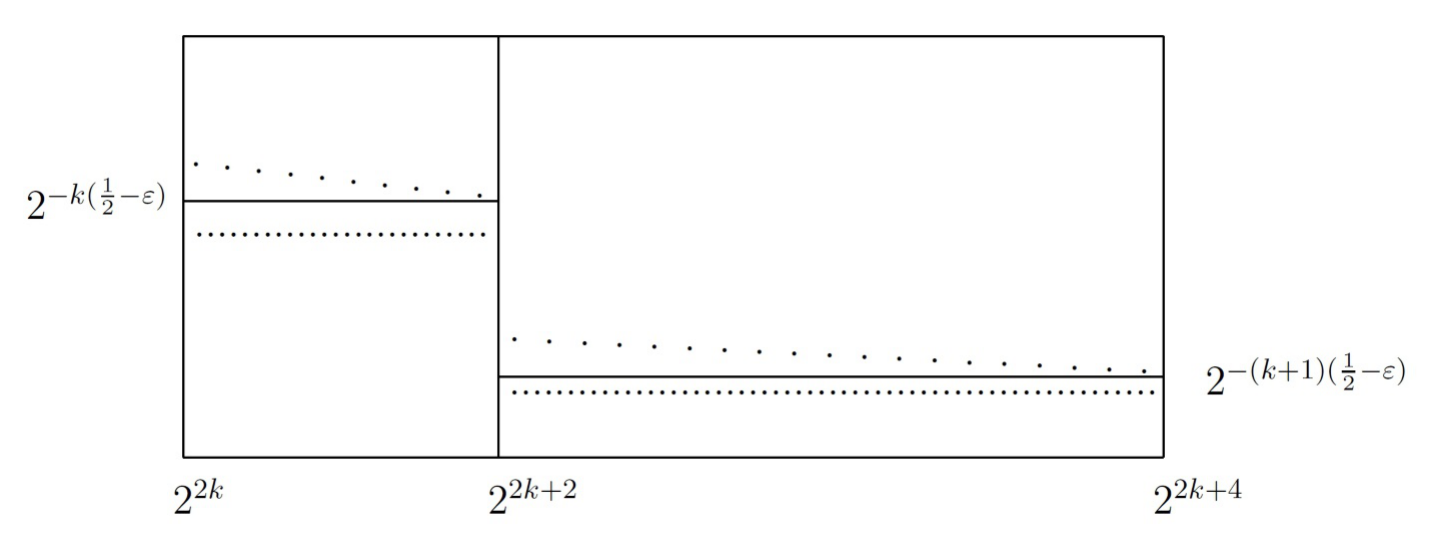
\includegraphics[width=0.78\textwidth]{figs/fig-8-sigma.png}
\end{center}

注意，对
\begin{equation}\label{eq:13}
  b_{k}=\frac{1}{2^{k\left(1/2-\varepsilon\right)}}\left(1+\frac{1}{j}\right),
\end{equation}
其中 $j = j(k)$ 满足 $2^{2k} \leq j < 2^{2k+2}$，由上面函数 $f$ 的定义，有
\begin{align*}
  \sum_{|\widehat{f}(\nu)|>b_{k}}\widehat{f}(\nu)e^{2\pi i\nu x}
  &=\sum_{|\nu|\leq 2^{2k}}\widehat{f}(\nu)e^{2\pi i\nu x}
   +\frac{1}{2^{k(1/2-\varepsilon)}}\sum_{2^{2k}\leq m^{2}<2^{2k}+j}
   \left(1+\frac{1}{m^{2}}\right)e^{2\pi i m^{2}x}.
\end{align*}
于是，当 $k \to \infty$ 时，回忆 Carleson--Hunt 收敛结果，对几乎所有 $x \in \R$,
\begin{equation}\label{eq:14}
  \Big|\sum_{|\widehat{f}(\nu)|>b_{k}}\widehat{f}(\nu)e^{2\pi i\nu x}\Big|
  =\frac{1}{2^{k(1/2-\varepsilon)}}\Big|\sum_{2^{2k}\leq m^{2}<2^{2k}+j}e^{2\pi i m^{2}x}\Big|
  +O(1).
\end{equation}
现在回忆下面的事实.

\begin{fact}\label{fact:8.17}
若 $|x - y| \leq 1/M^2$，则
\begin{align*}
  \sup_{1\leq k\leq M}\Big|\sum_{j=M}^{M+k}e^{2\pi i j^{2}x}\Big|
  \geq C\sup_{1\leq k\leq M}\Big|\sum_{j=M}^{M+k}e^{2\pi i j^{2}y}\Big|.
\end{align*}
\end{fact}

\begin{fact}\label{fact:8.18}
若 $\gcd(P, Q) = 1$，$M/2 \leq Q \leq M$ 且 $Q$ 为奇数，则
\begin{align*}
  \sup_{1\leq k\leq M}\Big|\sum_{j=M}^{M+k}e^{2\pi i j^{2}P/Q}\Big|\geq\sqrt{Q}.
\end{align*}
\end{fact}

事实 8.17 由分部求和得出，而事实 8.18 是定理 7.6 的推论.

我们将按 $x$ 构造 \eqref{eq:13} 中的序列 $b_k$. 设 $x \in [0,1]$ 是无理数，考虑其连分数展开的渐近分数序列 $\{P_m/Q_m\}$. 它们满足 $\gcd(P_m, Q_m) = 1$ 与
\begin{align*}
  \left|\frac{P_{m}}{Q_{m}}-x\right|<\frac{1}{Q_{m}^{2}}.
\end{align*}
奇数分母 $Q_{n}$ 有无穷多个.

奇数分母的（子）序列 $\{Q_{\alpha}\}$ 确定二进块
\begin{equation}\label{eq:15}
  2^{k_{\alpha}}\leq Q_{\alpha}\leq 2^{k_{\alpha}+1}.
\end{equation}
用这个指标序列 $\{k = k_\alpha\}$，考虑 \eqref{eq:13} 中的数 $b_k$，其中 $j = j(k)$ 选取为使
\begin{align*}
  \Big|\sum_{2^{2k}\leq m^{2}<2^{2k}+j}e^{2\pi i m^{2}x}\Big|
  =\sup_{1\leq\ell\leq 2^{k}}\Big|\sum_{s=2^{k}}^{2^{k}+\ell}e^{2\pi i s^{2}x}\Big|.
\end{align*}
先用事实 8.17，再用事实 8.18，得
\begin{align*}
  \sup_{1\leq\ell\leq 2^{k}}\Big|\sum_{s=2^{k}}^{2^{k}+\ell}e^{2\pi i s^{2}x}\Big|
  \geq C\sup_{1\leq\ell\leq 2^{k}}\Big|\sum_{s=2^{k}}^{2^{k}+\ell}e^{2\pi i s^{2}P_{\alpha}/Q_{\alpha}}\Big|
  \geq C\sqrt{Q_{\alpha}}.
\end{align*}
最后，由 \eqref{eq:14} 与 \eqref{eq:15}，得出
\begin{align*}
  \Big|\sum_{|\widehat{f}(\nu)|>b_{k}}\widehat{f}(\nu)e^{2\pi i\nu x}\Big|
  \geq C2^{k\varepsilon}+O(1).
\end{align*}
这证明函数 $f$ 满足 \eqref{eq:10} 中的几乎处处发散性质.

\subsection{范数中的收敛/发散}

还可以证明 $L^p$-收敛（$p < 2$）对 \eqref{eq:8.9} 的部分和 $\tilde{S}_\lambda$ 也失败. 更具体地，有下面.

\begin{theorem}\label{thm:8.19}
对所有 $p$，$1 \leq p < 2$，存在（显式构造的）函数 $f \in L^p(\T)$，使
\begin{align*}
  \limsup_{\lambda\to 0^{+}}\|\tilde{S}_{\lambda}f\|_{p}=\infty.
\end{align*}
\end{theorem}

这个函数的构造也是数论性质的，与上面展示的构造类似，但以素数指标扮演完全平方数的角色. 细节见 \cite{b182}.

可以论证，$\tilde{S}_{\lambda}f$ 收敛失败的一个原因是测不准原理未被考虑: 对 $|\widehat{f}(k)|$ 的大小施加限制而不对 $|k|$ 本身施加限制是没有意义的. 给定递减函数 $\phi$，可以考虑部分和:
\begin{align*}
  S_{N}^{\phi}f(x)=\sum_{\substack{|k|\leq N\\ |\widehat{f}(k)|\geq\phi(N)}}\widehat{f}(k)e^{2\pi i k x}.
\end{align*}
于是我们的构造表明，$S_{N}^{\phi}$ 在范数中收敛或发散的不同行为取决于条件
\begin{align*}
  N\cdot\phi^{2}(N)=o(1).
\end{align*}
特别地，对 $\phi(N) = N^{-\delta}$，$\delta > 0$，$S_{N}^{\delta}f$ 在 $L^{p}$-范数（$p < 2$）中的收敛
\begin{align*}
  S_{N}^{\delta}f(x)=\sum_{\substack{|k|\leq N\\ |\widehat{f}(k)|\geq N^{-\delta}}}\widehat{f}(k)e^{2\pi i k x}
\end{align*}
要求指数 $\delta > 1/2$，这与测不准原理相当吻合. 见 \cite{b182}.

% ================================================================
% 编号审计 (第 8 章):
%   question   ques:8.1  → 问题 8.1   (§8.1)
%   question   ques:8.2  → 问题 8.2   (§8.1)
%   definition def:8.3   → 定义 8.3   (§8.2，B_2[∞]-序列)
%   theorem    thm:8.4   → 定理 8.4   (§8.2)
%   lemma      lem:8.5   → 引理 8.5   (§8.2)
%   remark     rem:8.6   → 注 8.6     (§8.2)
%   proposition prop:8.7  → 命题 8.7   (§8.3)
%   lemma      lem:8.8   → 引理 8.8   (§8.3)
%   lemma      lem:8.9   → 引理 8.9   (§8.3)
%   remark     rem:8.10  → 注 8.10    (§8.4)
%   theorem    thm:8.11  → 定理 8.11  (§8.4，[176])
%   lemma      lem:8.12  → 引理 8.12 (Weyl 不等式) (§8.4)
%   lemma      lem:8.13  → 引理 8.13 (Vinogradov) (§8.4)
%   lemma      lem:8.14  → 引理 8.14 (大筛不等式) (§8.4)
%   theorem    thm:8.15  → 定理 8.15  (§8.4)
%   remark     rem:8.16  → 注 8.16    (§8.4)
%   fact       fact:8.17 → 事实 8.17 (§8.5)
%   fact       fact:8.18 → 事实 8.18 (§8.5)
%   theorem    thm:8.19  → 定理 8.19  (§8.5)
%   公式: eq:8.1 (§8.2 下界)，eq:8.2 (§8.2 断言)，eq:8.3 (§8.4 上界),
%         eq:8.4 (§8.4 A_h 界)，eq:8.5 (§8.4 A_h²)，eq:8.6 (§8.4 下界),
%         eq:8.7 (§8.4 Hölder 不等式)，eq:8.8 (§8.5 N-部分和),
%         eq:8.9 (§8.5 λ-部分和)，eq:8.10 (§8.5 发散性质),
%         eq:8.11 (§8.5 f_k)，eq:8.12 (§8.5 f)，eq:8.13 (§8.5 b_k),
%         eq:8.14 (§8.5 主项)，eq:8.15 (§8.5 二进块)
%   注: eq:8.10/8.11/8.12/8.13/8.14/8.15 的标签在原书中即 (8.10)-(8.15)；
%       本节无编号小标题"一个用高斯和的构造"用 \section*{}.
%   \cite 使用: b24 b171 b172 b173 b174 b175 b176 b180 b182 b184 b185
%               b187 b188 b189 b191 b192 b194 b195 b196
% ================================================================

% ================================================================
%  第 9 章 Weyl 和与原子能量振荡 (Weyl sums and atomic energy oscillations)
%  依据原书 PDF 第 201--246 页译出；编号审计见文件末尾注释
% ================================================================

\chapter{Weyl 和与原子能量振荡}

\epigraph{元素若按原子量排列，会呈现出性质上明显的周期性.}{Dmitri I. Mendeleev}

\section{目标陈述}

数学家天生是还原论者，常常梦想——也自诩——能够从一小套第一性原理严格推出科学的定律. 这是一个合理的目标，有着辉煌的历史，但极难实现. 而且它很少能打动物理学家，因为数学家能严格证明的东西通常不是他们的热点. 尽管如此，我们总可以引用 E.~Wigner 的评论: 数学作为物理理论表述与发展的基本工具，具有不合理的有效性.

我们从欧几里得那里学到，公理是不证自明的真理；但后来发现——先有 Gauss、Bólyai 与 Lobachevski，后有 Gödel 与连续统假设这个好例子——情况未必总是如此. 另一方面，物理学家常常愿意假设远离自明的新原理，唯一理由是它们极为有用. 薛定谔方程及其波函数解为给定系统的物理性质提供精确描述这一 ansatz 就是如此.

既然这是一本关于调和分析与傅里叶变换的书，似乎应该提及: ``测不准原理''——量子力学的一条基本原理——在好几章中扮演了重要角色: 主要在于这样的陈述: 若光滑函数在构型空间中适应于一个平行多面体（即它在每个方向的导数按平行多面体的相应边长衰减），则其傅里叶变换适应于动量空间中的一个对偶平行多面体，使得两者体积之积必须大于一个绝对常数（滥用语言的话，可以称之为 Planck 常数）. 第 6 章也考虑了通信理论中信号在时间与频率上不能同时受限这一不可能性. 感兴趣的读者可以参阅文献 \cite{b199,b205,b214,b213}，其中展开了傅里叶分析与量子力学中测不准原理的课题.

然而，不多说废话，让我们直接进入正题，声明在本章中我们将研究下面的和，它在非相对论原子能量的渐近分析中起关键作用:
\begin{align*}
  \Psi_{Q}(Z)=\sum_{l=1}^{l_{\mathrm{TF}}}\frac{2l+1}{
  \frac{1}{\pi}\int\bigl(V_{\mathrm{TF}}^{Z}(r)-\frac{l(l+1)}{r^{2}}\bigr)_{+}^{-1/2}\mathrm{d}r}
  \mu\Bigl(\frac{1}{\pi}\int\Bigl(V_{\mathrm{TF}}^{Z}(r)-\frac{l(l+1)}{r^{2}}\Bigr)_{+}^{1/2}\mathrm{d}r\Bigr),
\end{align*}
其中
\begin{align*}
  \mu(x)=\dist\{x,\Z\}^{2}-1/12,
\end{align*}
\begin{itemize}
\item $V_{\mathrm{TF}}^{Z}$ 是电荷为 $Z$ 的 Thomas--Fermi 位势，满足完美的标度条件
\begin{equation}\label{eq:9.1}
  V_{\mathrm{TF}}^{Z}(r)=Z^{4/3}V_{\mathrm{TF}}^{1}(Z^{1/3}r),
\end{equation}
并且有
\begin{equation}\label{eq:9.2}
  V_{\mathrm{TF}}^{1}(r)=\frac{y(ar)}{r},\qquad a=\left(\frac{3\pi}{2}\right)^{2/3},
\end{equation}
其中 $y$ 是 Thomas--Fermi 函数，即 Thomas--Fermi 方程
\begin{equation}\label{eq:9.3}
  \begin{cases}
    y^{\prime\prime}(r)=y^{3/2}(r)/\sqrt{r},\\
    y(0)=1,\\
    \lim_{r\to+\infty}y(r)=0,
  \end{cases}
\end{equation}
的解；

\item $l_{\mathrm{TF}}$ 是使 $V_{\mathrm{TF}}^{Z}(r) - l(l+1)/r^{2}$ 在某处为正的最大整数.
\end{itemize}
这里，记 $(x)_{+}^{-1/2} = x^{-1/2}$（若 $x > 0$），而在其他情形 $(x)_{+}^{-1/2} = 0$.

为理解函数 $\Psi_Q(Z)$ 在原子物理中的作用，让我们简要讨论非相对论分子的 Born--Oppenheimer 模型.

\section{Born--Oppenheimer 模型}

考虑
\begin{itemize}
\item 位于 $y_1, \ldots, y_M \in \R^3$ 的正电荷 $Z_1e, \ldots, Z_Me$ 的 $M$ 个原子核,
\begin{align*}
  Z=(Z_{1},\ldots,Z_{M}),\qquad Y=(y_{1},\ldots,y_{M});
\end{align*}
\item 位于 $x_1, \ldots, x_N \in \R^3$ 的 $N$ 个量子化电子；
\item $e$ = 电子电荷；$m$ = 电子质量；$\hbar$ = Planck 常数.
\end{itemize}
按照 Born--Oppenheimer 模型，非相对论分子由 Hamiltonian
\begin{align*}
  H_{Y,Z,N}=-\sum_{j=1}^{N}\Big(\frac{\hbar}{2m}\Delta_{x_{j}}+\sum_{k=1}^{M}\frac{Z_{k}e^{2}}{\left|x_{j}-y_{k}\right|}\Big)
  +\sum_{1\leq j<k\leq N}\frac{e^{2}}{\left|x_{j}-x_{k}\right|}
  +\sum_{1\leq m<n\leq M}\frac{Z_{n}Z_{m}e^{2}}{\left|y_{n}-y_{m}\right|},
\end{align*}
描述，其中第 $j$ 个 Laplacian 表示第 $j$ 个电子的量子化动能，还有库仑相互作用: 原子核与电子之间的吸引，以及两个排斥项——一个对应原子核之间，另一个对应电子之间.

这个 Hamiltonian 作用于
\begin{align*}
  \mathcal{H}=\bigwedge_{j=1}^{N}L^{2}(\R^{3}\otimes G),\qquad G=\left\{+1,-1\right\}.
\end{align*}
这里，符号 $\wedge$ 表示反对称张量积，编码了 Pauli 不相容原理（电子是满足 Fermi--Dirac 统计的\newterm{fermion}{费米子}{fermion}）；而 $+1$（自旋向上）与 $-1$（自旋向下）表示电子自旋的两种.

\newterm{ground-state-energy}{基态能量}{ground state energy}由
\begin{align*}
  E(Z)=\inf_{N}\inf_{Y}\inf_{\substack{\Psi\in\mathcal{H}\\ \|\Psi\|=1}}\langle\Psi,H_{Y,Z,N}\Psi\rangle
\end{align*}
给出.

要实现用数学解释化学现象的梦想，需要对这些能量作非常精确的计算，而这一任务的难度比今天所能达到的高出好几个量级.

下面，我们将面对更``谦逊''的目标: 迈出解释周期表的第一步，为此只需考虑中性原子的 Hamiltonian 就够了.

\section{中性原子. Hartree--Fock 理论与 Thomas--Fermi 理论}

考虑一个在原点 $y = 0$ 处有 $Z$ 个质子的中性\newterm{atom}{原子}{atom}，并选取单位使 $e^2 = 1$ 且 $\hbar/2m = 1$. 则
\begin{align*}
  H_{Z}=-\sum_{j=1}^{Z}\left(\Delta_{x_{j}}+\frac{Z}{\left|x_{j}\right|}\right)
  +\sum_{1\leq j<k\leq Z}\frac{1}{\left|x_{j}-x_{k}\right|}.
\end{align*}
尽管自旋变量在描述电子行为时是根本的，但从理解数学模型的角度看它们无关紧要. 因此，可以在讨论中省略它们，把态 Hilbert 空间的结构简化为
\begin{align*}
  \mathcal{H}=\bigwedge_{j=1}^{Z}L^{2}(\R^{3})
  =\{\Psi(x_{1},\ldots,x_{Z}),\ x_{j}\in\R^{3}:
  \Psi\in L^{2}(\R^{3Z}),\ \Psi\ \text{反对称}\}.
\end{align*}
反对称意味着对每个置换 $\sigma$，$\Psi(x_{\sigma(1)},\ldots,x_{\sigma(Z)}) = (-1)^{\operatorname{sign}(\sigma)}\Psi(x_1,\ldots,x_Z)$.

电子密度由
\begin{align*}
  \rho(x)=Z\int_{\R^{3(Z-1)}}\left|\Psi(x,x_{2}\ldots,x_{Z})\right|^{2}\,\mathrm{d}x_{2}\cdots\mathrm{d}x_{Z}
\end{align*}
给出，因而
\begin{align*}
  \int_{\Omega}\rho(x)\,\mathrm{d}x
\end{align*}
是 $\Omega \subset \R^3$ 中电子的期望数.

基态能量现在写成
\begin{align*}
  E(Z)=\inf_{\substack{\Psi\in\mathcal{H}\\ \|\Psi\|=1}}\langle\Psi,H_{Z}\Psi\rangle.
\end{align*}
因此，任务在于得到 Hamiltonian $H_{Z}$ 作用于 $3Z$ 维欧氏空间中反对称平方可积函数上的最低特征值. 但这仍然是一个非常困难的问题，主要由于电子的库仑相互作用.

从量子力学的最初年代起，人们就知道显式求解薛定谔方程 $H_{Z}\Psi = \lambda\Psi$ 是不可能的，于是引入了若干近似解法.

若我们的 Hamiltonian 对单电子位势 $V$ 有形如
\begin{align*}
  \widetilde{H}_{Z}=\sum_{k=1}^{Z}\left(-\Delta_{x_{k}}+V(x_{k})\right)
\end{align*}
的形式，则由分离变量，问题将从 $3Z$ 维化归为 $3$ 维. 此外，利用径向对称性，它将变成纯一维（即常微分方程），容易求解.

在量子理论（物理学与化学）中引入的研究原子的主要思想，是用 $\tilde{H}_Z$ 近似 $H_Z$，其中位势 $V(x)$ 选取如下: 让我们暂时假装知道电子密度 $\rho$；那么这样的单电子位势的一个好候选是
\begin{align*}
  V(x)=-\frac{Z}{\left|x\right|}+\int_{\R^{3}}\frac{\rho(y)}{\left|x-y\right|}\,\mathrm{d}y.
\end{align*}
容易推出，$\widetilde{H}_{Z}$ 的基态本征函数与基态电子密度由下面给出:
\begin{itemize}
\item $\Psi_{HF}(x_1,\ldots,x_Z)$，即三维 Schrödinger 算子 $-\Delta + V(x)$ 的本征函数 $\phi_1(x),\ldots,\phi_Z(x)$ 的反对称化乘积（Slater 行列式）；
\begin{align*}
  \rho_{\mathrm{HF}}(x)=\sum_{k=1}^{Z}|\phi_{k}(x)|^{2}.
\end{align*}
\end{itemize}
这一方法（Hartree--Fock）是对原问题的一大简化，因为现在我们面对的只是三维计算而非 $3Z$ 维. 系统通过要求一致性条件（Hartree--Fock 方程）——所得密度等于初始密度——而封闭:
\begin{align*}
  \rho_{\mathrm{HF}}=\rho.
\end{align*}
这是一个引人注目而奇特的方程（既非代数方程、偏微分方程，也非积分方程），通过迭代求解: 从初始密度 $\rho_0$ 出发，产生 Hartree--Fock $\rho_1$；把它作为新的初始数据产生 $\rho_2$，如此继续. 极限密度（假设它存在）将是我们寻求的解.

在这个设定下，容易推出 Hartree--Fock 基态正如上面所指出的，由本征函数的反对称化乘积给出，且负特征值之和是 Hamiltonian 的最低可能能量.

方法是否可行并不显然，无论如何，收敛将依赖于适当初始密度的选取. 在这里，也称原子统计理论的 Thomas--Fermi 理论前来相助，为我们提供三维 Schrödinger 算子的密度与特征值和的良好第一步近似.

Thomas--Fermi 理论是一种用于处理多粒子系统量子力学的技术. 当 $Z$ 很大时，无法指望理解通常的\newterm{wave-function}{波函数}{wave function} $\Psi(x_1, \ldots, x_Z)$. 取而代之，人们试图理解电子密度
\begin{align*}
  \rho(x_{1})=Z\int|\Psi(x_{1},x^{\prime})|^{2}\,\mathrm{d}x^{\prime},
\end{align*}
它是 $x_1 \in \R^3$ 的函数，并希望关于 $\Psi$ 的重要信息都包含在 $\rho = \rho_{\mathrm{TF}}^Z$ 中.

Thomas--Fermi 理论推导出描述 $\rho_{\mathrm{TF}}^{Z}$ 的一个偏微分方程，并从电子密度 $\rho_{\mathrm{TF}}^{Z}$ 的知识猜测系统的能量，见 \cite{b221}. 它把量子力学视为充满相空间、通过库仑排斥与自身相互作用并与位势
\begin{align*}
  V_{\mathrm{TF}}^{Z}(x)=-\frac{Z}{\left|x\right|}+\frac{1}{2}\int_{\R^{3}}\frac{\rho_{\mathrm{TF}}^{Z}(y)}{\left|x-y\right|}\mathrm{d}y
\end{align*}
相互作用的经典气体，该位势满足 \eqref{eq:9.1}--\eqref{eq:9.3} 描述的 Thomas--Fermi 方程；在径向对称性假设下，这些方程变成一个可以求解的非线性常微分方程，表明对参数 $Z$ 的依赖可以通过平凡标度去掉:
\begin{align*}
  \rho_{\mathrm{TF}}^{Z}(x)=Z^{2}\;\rho(Z^{1/3}x),\qquad
  V_{\mathrm{TF}}^{Z}(x)=Z^{4/3}\;V(Z^{1/3}x),
\end{align*}
其中密度 $\rho$ 与位势 $V$ 是完全确定的函数. 这些公式在``原子半径''$Z^{-1/3}$ 与电子间平均距离 $Z^{-2/3}$ 的意义下有自然的解释.

数学中一个成熟悠久的传统是用线性方程近似非线性方程. Thomas--Fermi 与 Hartree--Fock 方法涉及用少数变量的非线性系统近似大量变量的线性系统，见 \cite{b221}.

\begin{remark*}
推导 Thomas--Fermi 方程的关键一步是用电子密度函数表示动能:
\begin{align*}
  \mathcal{E}_{\mathrm{KE}}=C_{\mathrm{TF}}\int\rho^{5/3}(x)\,\mathrm{d}x,
\end{align*}
从而总能量为
\begin{align*}
  \mathcal{E}_{\mathrm{TF}}=C_{\mathrm{TF}}\int\rho^{5/3}(x)\,\mathrm{d}x
  -\int V(x)\rho(x)\,\mathrm{d}x
  +\frac{1}{2}\iint\frac{\rho(x)\rho(y)}{|x-y|}\,\mathrm{d}x\,\mathrm{d}y.
\end{align*}
见 \cite{b221}.
\end{remark*}

为给 Thomas--Fermi 关于 $\mathcal{E}_{\mathrm{KE}}$ 的 ansatz 提供动机，并与第 7 章的格点问题建立有趣的联系，下面我们将描述一个由 $\R^3$ 中 $\delta$-盒 $B_{\delta} = [0, \delta] \times [0, \delta] \times [0, \delta]$ 内 $N$ 个自由粒子组成的玩具模型. 即，假设它们彼此不施力，然后寻找这些粒子所具有的基态能量，它由\newterm{wave-function}{波函数}{wave function} $\Psi(x_1, \ldots, x_N)$ 给出.

注意 $\Psi$ 支于 $B_{\delta} \times \cdots \times B_{\delta} = B_{\delta}^{(N)}$，满足
\begin{align*}
  \int_{B_{\delta}^{(N)}}|\Psi(x_{1},\ldots,x_{N})|^{2}=1,\qquad
  \mathcal{E}_{\mathrm{QE}}=\langle-\Delta\Psi,\Psi\rangle,
\end{align*}
而 $\rho(x_1) = N\int |\Psi(x_1, x')|^2\,\mathrm{d}x'$ 是粒子密度.

再假设\newterm{wave-function}{波函数}{wave function} $\Psi$ 是反对称的（Pauli 不相容原理），然后求能量最小的态，即基态.

设 $f_1, f_2, \ldots$ 是 $-\Delta$ 在 $B_\delta$ 中 Dirichlet 边界条件下的本征函数，$\lambda_1, \lambda_2, \ldots$ 是相应的特征值. 由于 $\R^{3N}$ 中的 Laplacian 经分离变量分裂，我们问题的本征函数将是
\begin{align*}
  \Psi_{m_{1},\ldots,m_{N}}(x_{1},\ldots,x_{N})=f_{m_{1}}(x_{1})\cdots f_{m_{N}}(x_{N}),
\end{align*}
特征值为 $\lambda_{m_1} + \cdots + \lambda_{m_N}$.

考虑到反对称性，若希望 $\Psi$ 不恒等于零，必须选取不同的 $m_j$. 于是得到反对称本征函数
\begin{align*}
  \Psi_{m_{1},\ldots,m_{N}}(x_{1},\ldots,x_{N})
  =\frac{1}{N!}\sum_{\sigma\in S_{N}}\operatorname{sign}(\sigma)f_{m_{1}}(x_{1})\cdots f_{m_{N}}(x_{N}),
\end{align*}
其中和对对称群 $S_{N}$ 的所有元素 $\sigma$ 进行.

但我们在盒 $B_{\delta}$ 中显式地知道这些本征函数；它们是
\begin{align*}
  \prod_{j=1}^{3}\sin\Bigl(\frac{\pi\nu_{j}\cdot x_{j}}{\delta}\Bigr),\qquad
  \nu_{j}=(\nu_{j}^{1},\nu_{j}^{2},\nu_{j}^{3})\in\Z^{3},
\end{align*}
相应的特征值是
\begin{align*}
  \frac{\pi^{2}}{\delta^{2}}\left((\nu_{j}^{1})^{2}+(\nu_{j}^{2})^{2}+(\nu_{j}^{3})^{2}\right)
  =\frac{\pi^{2}}{\delta^{2}}|\nu_{j}|^{2}.
\end{align*}
为估计前几个特征值之和，取一个包含 $N$ 个格点（也许除小误差外）的半径 $r$ 的球，并注意
\begin{align*}
  N\simeq\operatorname{vol}\{|\xi|<r:\xi_{j}\geq 0\}\simeq r^{3}.
\end{align*}
因此，能量为
\begin{align*}
  \simeq\int_{|\xi|<r,\ \xi_{j}>0}\frac{\pi^{2}}{\delta^{2}}|\xi|^{2}\,\mathrm{d}\xi=C\frac{r^{5}}{\delta^{2}},
\end{align*}
把它写成
\begin{align*}
  C\left(\frac{N}{\delta^{3}}\right)^{5/3}\delta^{3}.
\end{align*}
但 $N/\delta^{3}$ 是盒 $B_{\delta}$ 中的粒子密度，$\delta^{3}$ 是体积. 因此，把空间分成小盒 $B_{\delta}^{k}$——其中 $\rho = \rho_{k}$ 近似为常数——把所有上述项相加，并在粒子数 $N$ 足够大时取极限，就得到所寻求的动能表达式
\begin{align*}
  C_{\mathrm{TF}}\int\rho^{5/3}(x)\,\mathrm{d}x.
\end{align*}
该公式的精确推导以及 Hartree--Fock 方程更易处理的形式，见 \cite{b221,b220}.

\section{原子的基态能量}

上面的文字只是呈现此处要点所需的 Hartree--Fock 与 Thomas--Fermi 理论的粗略印象式概述；要点是对原子基态能量的严格（数学定理）结果，它可以总结为下面的（渐近）展开:
\begin{align*}
  E(Z)=C_{\mathrm{TF}}Z^{7/3}+C_{\mathrm{s}}Z^{2}+C_{\mathrm{sd}}Z^{5/3}+\Psi_{Q}(Z)+\cdots.
\end{align*}
\begin{itemize}
\item 项 $C_{\mathrm{TF}}Z^{7/3}$ 于 1927 年由 Thomas--Fermi \cite{b212,b226} 提出，于 1977 年由 Lieb--Simon \cite{b221} 证明.
\item 项 $C_sZ^2$ 首先出现在数值计算中，于 1952 年由 Scott \cite{b222} 解释，并由 Hughes--Siedentop--Weikard 于 1985--89 年 \cite{b224,b225,b218} 严格证明. 它反映了靠近原子核的电子行为仿佛没有电子相互作用（屏蔽效应）.
\item 项 $C_{\mathrm{SD}}Z^{5/3}$ 于 1930 年由 Dirac \cite{b203}、1981 年由 Schwinger \cite{b223} 猜想. 它于 1990 年由 Fefferman--Seco \cite{b207} 证明. 它代表由微妙的电子关联引起的小效应.
\end{itemize}
下一项 $\Psi_Q(Z)$ 是振荡的，由前面陈述过的公式给出:
\begin{align*}
  \Psi_{Q}(Z)=\sum_{l=1}^{l_{\mathrm{tr}}}\frac{2l+1}{
  \frac{1}{\pi}\int\mathcal{F}(r)^{-1/2}\,\mathrm{d}r}
  \cdot\mu\Bigl(\frac{1}{\pi}\int\mathcal{F}(r)^{1/2}\,\mathrm{d}r\Bigr),
\end{align*}
其中
\begin{align*}
  \mathcal{F}(r):=\left(V_{\mathrm{TF}}^{Z}(r)-\frac{l(l+1)}{r^{2}}\right)_{+},
\end{align*}
约定 $x \leq 0$ 时 $(x)_{+} = 0$，其中
\begin{align*}
  V_{\mathrm{TF}}^{Z}(r)=Z^{4/3}V(Z^{1/3}r)
\end{align*}
是 Thomas--Fermi 位势，而
\begin{align*}
  l_{\mathrm{TF}} = \{\text{使 } V_{\mathrm{TF}}^{Z}(r) - l(l + 1)/r^{2} > 0 \text{ 在某处成立的最大整数 } l\}.
\end{align*}
最后,
\begin{align*}
  \mu(x)=\dist(x,\Z)^{2}-\frac{1}{12}.
\end{align*}
$\mu(x)$ 的图象如下所示.

\begin{center}
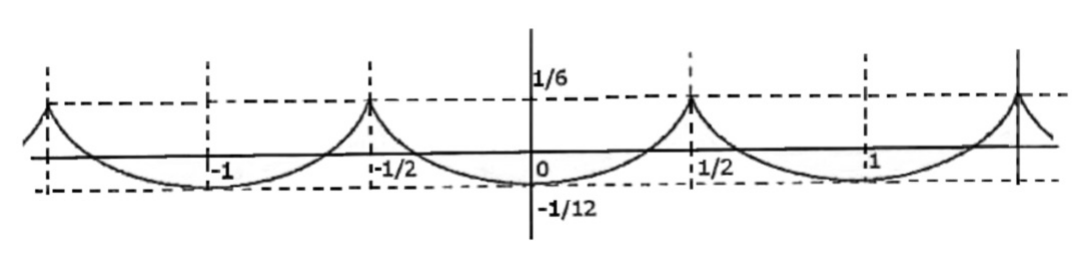
\includegraphics[width=0.6\textwidth]{figs/fig-9-energy.png}
\end{center}

$\Psi_Q$ 的振荡（殆周期的）特征非常有趣，有相当的理由相信它编码了价电子对能量的贡献. 我们对这一项的分析包含在下面的定理中.

\begin{theorem}\label{thm:9.1}
\begin{align*}
  -c_{1}Z^{3/2}\leq\Psi_{Q}(Z)\leq c_{1}Z^{3/2},\qquad
  \Bigl(\frac{1}{Z}\int_{1}^{Z}|\Psi_{Q}(u)|^{2}\,\mathrm{d}u\Bigr)^{1/2}\geq c_{2}Z^{3/2},
\end{align*}
其中 $0 < c_1, c_2 < \infty$ 是普适常数.
\end{theorem}

特别地，有
\begin{align*}
  |\Psi_{Q}| \text{ 的平均} \approx Z^{3/2}.
\end{align*}

本章其余部分将致力于给出定理 9.1 证明的细节. 这是一个冗长的论证，涉及一系列类似的振荡积分计算，采用驻相法、van der Corput 估计与泊松求和公式等技术. 在某种意义上，如引言中所指出的，它位于第 1 章数学俳句的对跖点.

对精通原子数学理论、熟悉文献 \cite{b208,b209,b218,b221} 内容的读者，本章将提供对基态能量渐近展开中这个引人入胜的振荡项的估计的全面阐述. 然而，对那些不熟悉 Hartree--Fock 与 Thomas--Fermi 模型、但对前面各章的调和分析感兴趣的读者，深入这个证明的细节可以进一步坚定他们对这一领域作为描述自然现象的合适工具之力量的信念. 还可以认为，它作为激励去探索上述文献中丰富而有力的数学，并且也许将促进数学梦想中``以几何方式证明''（more geometrico demonstrata）化学的进展，正如 Spinoza 会说的那样.

在我们的分析中，首先解码它的表达式，强调它与数论中一些经典公式的类比，即欧氏空间区域内数格点问题中出现的那些公式. 然后我们可以利用数论学家为处理三角和而引入的工具来完成定理的证明.

从抽象数学的角度看，诸如 $\Psi_Q$ 的和相当古老，最著名的可上溯至 Gauss，它与估计凸区域内整格点数有关，如第 7 章所考虑的.

值得注意我们的问题与圆问题之间的密切相似性，后者来自对盒中量子自由粒子束缚态数目的精细分析.

证明组织如下. 首先，在对众所周知的驻相引理作一些平凡修改之后（9.5 节），我们（在 9.6 节）着手研究形如
\begin{align*}
  S(\lambda)=\sum_{l=1}^{\lambda}f\Big(\frac{l}{\lambda}\Big)\mu\Big(\lambda\phi\Big(\frac{l}{\lambda}\Big)\Big)
\end{align*}
的和，其中 $\phi''(x) \geq c_0 > 0$，$\mu$ 是平均为 $0$ 的周期函数. 这类和的例子如下.

\begin{enumerate}
\item 若 $f \equiv 1$，$\mu(x) = e^{2\pi ix}$，$\phi(x) = x^2$，则得到模 $\lambda$ 的著名 Gauss 和.
\item 若 $f \equiv 1$，$\mu(x) = x - [x] - 1/2$，则 $S$ 表示被 $\lambda$ 膨胀的曲线 $\phi$ 的格点问题中的误差项.
\end{enumerate}

虽然上面第一项已被充分理解，第二项仍然非常困难. 在我们的情形中，只需处理傅里叶系数衰减相当快（$\hat{\mu}(n) \sim |n|^{-3/2+\varepsilon}$）的函数 $\mu$，这允许用 van der Corput 的通常方法（泊松求和接驻相法；见 \cite{b215}）对这些和作完全分析，因为所有表达式都绝对收敛. 这里还需要一点初等数论论证来排除小分母问题的可能性，它产生一个大小依赖于某个数是有理数还是无理数的误差项.

在 9.7 节中，我们把 9.6 节的结果应用于 $\Psi_Q$，得到一个新的和 $\Psi_0$，即 $\Psi_Q$ 的领头``对偶''版本，令人想起模函数的 Jacobi 恒等式. $\Psi_Q$ 的精确上界是它的容易推论. 然而，为得到 $\Psi_Q$ 公式中所涉曲线与振幅的正确正则性性质，结果相当繁琐.

在 9.8 节中，通过理解 $\Psi_0$ 在平均意义下的行为，我们以 $\Omega$-结果的形式得到 $\Psi_Q$ 的下界.

这些结果最初发表于 \cite{b200,b201}，以下数页几乎是这些论文内容的逐字转录，它们严重依赖 \cite{b208} 中证明的估计.

\section{驻相估计}

让我们从回顾驻相开始. 考虑 $f \in C_0^\infty(\R)$. 则若 $t > 0$,
\begin{align*}
  \int_{-\infty}^{\infty}e^{i t x^{2}}f(x)\,\mathrm{d}x
  =e^{\pi i/4}\sqrt{\frac{\pi}{t}}\int_{-\infty}^{\infty}e^{-\pi^{2}i\xi^{2}/t}\widehat{f}(\xi)\,\mathrm{d}\xi.
\end{align*}
利用恒等式
\begin{align*}
  e^{s}=1+\int_{0}^{1}e^{su}s\,\mathrm{d}u,
\end{align*}
推出
\begin{equation}\label{eq:9.4}
  \begin{aligned}
  \int_{-\infty}^{\infty}e^{itx^{2}}f(x)\,\mathrm{d}x
  &=e^{\pi i/4}\sqrt{\frac{\pi}{t}}\left(f(0)+\int_{-\infty}^{\infty}\widehat{f}(\xi)
   \int_{0}^{1}\frac{-\pi^{2}i\xi^{2}}{t}e^{-\pi^{2}iu\xi^{2}/t}\,\mathrm{d}u\,\mathrm{d}\xi\right)\\
  &=e^{\pi i/4}\sqrt{\frac{\pi}{t}}\left(f(0)+\frac{i}{4t}\int_{-\infty}^{\infty}\widehat{f^{\prime\prime}}(\xi)
   \int_{0}^{1}e^{-\pi^{2}iu\xi^{2}/t}\,\mathrm{d}u\,\mathrm{d}\xi\right)\\
  &=e^{\pi i/4}\sqrt{\frac{\pi}{t}}f(0)+\frac{i}{4t}\int_{-\infty}^{\infty}f^{\prime\prime}(x)
   \int_{0}^{1}e^{itx^{2}/u}\frac{\mathrm{d}u}{u^{1/2}}\,\mathrm{d}x\\
  &=e^{\pi i/4}\sqrt{\frac{\pi}{t}}f(0)+\frac{i}{4t^{3/2}}\int_{-\infty}^{\infty}f^{\prime\prime}(x)g_{t}(x)\,\mathrm{d}x,
  \end{aligned}
\end{equation}
其中
\begin{align*}
  g_{t}(x)=\int_{0}^{1}e^{itx^{2}/u}\left(\frac{t}{u}\right)^{1/2}\mathrm{d}u.
\end{align*}
注意 $g_{t}(x)=t^{1/2}g_{1}(t^{1/2}x)$，且
\begin{align*}
  g_{1}(x)=i\,e^{i x^{2}/u}\frac{u^{3/2}}{x^{2}}\Big|_{0}^{1}-\frac{3i}{2}\int_{0}^{1}e^{i x^{2}/u}\frac{u^{1/2}}{x^{2}}\,\mathrm{d}u,
\end{align*}
因此 $|g_1(x)| \leq 2/|x|^2$，从而 $g_1$ 可积. 此外,
\begin{align*}
  \|g_{t}\|_{1}=\|g_{1}\|_{1}=O(1),\qquad
  |g_{t}(x)|\leq 2|x|^{-2}t^{-1/2}.
\end{align*}
我们还考虑形如
\begin{align*}
  \int_{0}^{\infty}e^{itx^{2}}f(x)\,\mathrm{d}x
\end{align*}
的单侧积分. 定义
\begin{align*}
  f^{+}(x)=\begin{cases}
    f(x), & \text{若 } x\geq 0,\\
    f(-x), & \text{若 } x\leq 0,
  \end{cases}
\end{align*}
并考虑 $f_{\varepsilon} = f^{+} * \varphi_{\varepsilon}$，其中 $\varphi_{\varepsilon}$ 是恒等算子的适当逼近. 用我们之前的恒等式，得
\begin{align*}
  &\int_{0}^{\infty}e^{itx^{2}}f(x)\,\mathrm{d}x\\
  &=\frac{1}{2}\lim_{\varepsilon\rightarrow 0}\int_{-\infty}^{\infty}e^{itx^{2}}f_{\varepsilon}(x)\,\mathrm{d}x
  =\frac{1}{2}e^{\pi i/4}\sqrt{\frac{\pi}{t}}f(0)
   +\frac{i}{8t^{3/2}}\lim_{\varepsilon\rightarrow 0}\int_{-\infty}^{\infty}f_{\varepsilon}^{\prime\prime}(x)g_{t}(x)\,\mathrm{d}x\\
  &=\frac{1}{2}e^{\pi i/4}\sqrt{\frac{\pi}{t}}f(0)
   +\frac{i}{4t^{3/2}}\int_{0}^{\infty}f^{\prime\prime}(x)g_{t}(x)\,\mathrm{d}x.
\end{align*}
最后一步成立是因为 $g_{t}$ 可积，且函数 $g_{t}$ 与 $f^{+}$ 都为偶.

\begin{definition}\label{def:9.2}
设 $\phi$ 满足
\begin{align*}
  |\phi^{(n)}(x)|\leq C_{n}\quad (0\leq n\leq 5),\qquad
  c_{0}=\inf|\phi^{\prime\prime}(x)|>0,
\end{align*}
对某个在应用中会明确的区间中的 $x$ 成立. 记
\begin{align*}
  c_{0}^{+}=\min\{1,c_{0}\},\qquad
  B(\phi)=\left(\frac{1+\|\phi\|_{C^{5}}}{c_{0}^{+}}\right)^{54}.
\end{align*}
\end{definition}

\begin{lemma}[驻相引理]\label{lem:9.3}
设 $f(x) \in C_0^2(\R)$ 满足
\begin{align*}
  \left|f^{\prime}(x)\right|\leq\begin{cases}
    N_{1}, & \text{若 } \left|x\right|\leq L,\\
    N_{2}, & \text{若 } \left|x\right|>L,
  \end{cases}
  \qquad
  \left|f^{\prime\prime}(x)\right|\leq\begin{cases}
    M_{1}, & \text{若 } \left|x\right|\leq L,\\
    M_{2}, & \text{若 } \left|x\right|>L,
  \end{cases}
\end{align*}
其中 $N_{1} \leq N_{2}$，$M_{1} \leq M_{2}$；设 $\phi(x)$ 满足 $\phi(0) = \phi'(0) = 0$，对 $0 \leq n \leq 5$ 有 $|\phi^{(n)}(x)| \leq C_{n}$，且对 $f$ 支集中的所有 $x$ 有 $\phi''(x) \geq c_{0} > 0$. 则
\begin{equation}\label{eq:9.5}
  \begin{aligned}
  &\Big|\int_{-\infty}^{\infty}e^{it\phi(x)}f(x)\,\mathrm{d}x
   -\Big(\frac{2\pi}{|t|\phi^{\prime\prime}(0)}\Big)^{1/2}e^{\operatorname{sign}(t)\pi i/4}f(0)\Big|\\
  &\quad\leq AB(\phi)t^{-3/2}\Big(\|f\|_{\infty}+N_{1}+\frac{N_{2}}{t^{1/2}L}+M_{1}+\frac{M_{2}}{t^{1/2}L}\Big).
  \end{aligned}
\end{equation}
类似地,
\begin{equation}\label{eq:9.6}
  \begin{aligned}
  &\Big|\int_{0}^{\infty}e^{it\phi(x)}f(x)\,\mathrm{d}x
   -\Big(\frac{\pi}{2|t|\phi^{\prime\prime}(0)}\Big)^{1/2}e^{\operatorname{sign}(t)\pi i/4}f(0)\Big|\\
  &\quad\leq AB(\phi)t^{-3/2}\Big(\|f\|_{\infty}+N_{1}+\frac{N_{2}}{t^{1/2}L}+M_{1}+\frac{M_{2}}{t^{1/2}L}\Big).
  \end{aligned}
\end{equation}
还有通常的与 $L$ 无关的估计
\begin{equation}\label{eq:9.7}
  \begin{aligned}
  \Big|\int_{-\infty}^{\infty}e^{it\phi(x)}f(x)\,\mathrm{d}x
  &-\Big(\frac{2\pi}{|t|\phi^{\prime\prime}(0)}\Big)^{1/2}e^{\operatorname{sign}(t)\pi i/4}f(0)\Big|\\
  &\leq AB(\phi)t^{-3/2}\left(\|f\|_{\infty}+\|f^{\prime}\|_{1}+\|f^{\prime\prime}\|_{1}\right),
  \end{aligned}
\end{equation}
以及
\begin{equation}\label{eq:9.8}
  \begin{aligned}
  &\Big|\int_{0}^{\infty}e^{it\phi(x)}f(x)\,\mathrm{d}x
   -\Big(\frac{\pi}{2|t|\phi^{\prime\prime}(0)}\Big)^{1/2}e^{\operatorname{sign}(t)\pi i/4}f(0)\Big|\\
  &\qquad\leq AB(\phi)t^{-3/2}\left(\|f\|_{\infty}+\|f^{\prime}\|_{1}+\|f^{\prime\prime}\|_{1}\right),
  \end{aligned}
\end{equation}
其中 $A$ 是普适常数，$B(\phi)$ 如上定义，对 $f$ 支集中的 $x$ 取值.

这里，$\operatorname{sign}(t)$ 表示这样的函数: $t > 0$ 时等于 $1$，$t < 0$ 时等于 $-1$.
\end{lemma}

\begin{proof}
显然只须考虑 $t > 0$ 的情形. 考虑由
\begin{align*}
  u(x)=x\sqrt{\frac{\phi(x)}{x^{2}}}
\end{align*}
给出的变量替换及其逆 $z(u)$. 首先得到 $u$ 与 $z$ 的正则性性质.

设 $k \geq 1$. 下面，$A_k$ 表示只依赖于 $k$ 的普适常数族. 首先考虑 $|x| \leq 1$，定义
\begin{align*}
  \phi_{1}(x)=x^{-2}\phi(x).
\end{align*}
由于
\begin{align*}
  \phi_{1}(x)=\int_{0}^{1}\int_{0}^{1}\phi^{\prime\prime}(s t x)\,s\,\mathrm{d}t\,\mathrm{d}s,
\end{align*}
有
\begin{align*}
  \|\phi_{1}\|_{C^{k}}\leq A_{k}\|\phi\|_{C^{k+2}}.
\end{align*}
其次，定义
\begin{align*}
  \phi_{2}(x)=\sqrt{\phi_{1}(x)},\qquad |x|\leq 1,
\end{align*}
并注意
\begin{align*}
  \frac{d^{k}\phi_{2}(x)}{d x^{k}}
  =\frac{1}{\phi_{1}^{k-1/2}(x)}\sum_{\substack{1\cdot i_{1}+\cdots+p\cdot i_{p}=k\\ i_{j}\geq 0}}
  c_{i_{1},\ldots,i_{p}}^{(k)}\phi_{1}^{\prime}(x)^{i_{1}}\cdots\phi_{1}^{(p)}(x)^{i_{p}},
\end{align*}
这可以用归纳容易地验证，且是归功于 F.~Faà di Bruno 的著名公式的一个特殊情形. 结果,
\begin{align*}
  \|\phi_{2}\|_{C^{k}}\leq A_{k}\frac{(1+\|\phi_{1}\|_{C^{k}})^{k}}{c_{0}^{k-1/2}}
  \leq A_{k}\frac{(1+\|\phi\|_{C^{k+2}})^{k}}{c_{0}^{k-1/2}},
\end{align*}
其中用到了 $\phi_1(x) \geq c_0/2$ 的事实. 于是，由于 $u(x) = x\phi_2(x)$，得出
\begin{align*}
  \left|\frac{d^{k}u(x)}{d x^{k}}\right|
  \leq A_{k}\frac{(1+\|\phi\|_{C^{k+2}})^{k}}{(c_{0}^{+})^{k-1/2}},\qquad |x|\leq 1.
\end{align*}
当 $|x| > 1$ 时，显然有
\begin{align*}
  \frac{d^{k}u(x)}{d x^{k}}
  =\sum_{i=1}^{k}\phi^{1/2-i}(x)\sum_{\substack{1\cdot i_{1}+\cdots+p\cdot i_{p}=k\\ i_{j}\geq 0}}
  c_{i_{1},\ldots,i_{p}}^{i,k}\phi^{\prime}(x)^{i_{1}}\cdots\phi^{(p)}(x)^{i_{p}},
\end{align*}
因此
\begin{align*}
  |u^{(k)}(x)|\leq A_{k}\frac{(1+\|\phi\|_{C^{k}})^{k}}{(c_{0}^{+})^{k-1/2}},\qquad |x|>1,
\end{align*}
所以合起来得到
\begin{align*}
  \|u\|_{C^{k}}\leq A_{k}\frac{(1+\|\phi\|_{C^{k+2}})^{k+2}}{(c_{0}^{+})^{k-1/2}}.
\end{align*}
最后，由于
\begin{align*}
  z^{\prime}(u(x))u^{\prime}(x)=1,
\end{align*}
且对 $k \geq 2$,
\begin{align*}
  \frac{\mathrm{d}^{k}z}{\mathrm{d}u^{k}}(u(x))(u^{\prime}(x))^{k}
  =\sum_{p=1}^{k-1}K_{k,p}\frac{\mathrm{d}^{p}z}{\mathrm{d}u^{p}}(u(x))
  \sum_{\substack{1\cdot i_{1}+\cdots+q\cdot i_{q}=k+1-p\\ i_{j}>0}}
  c_{i_{2},\ldots,i_{q}}^{k,p}u^{\prime}(x)^{i_{1}}\cdots u^{(q)}(x)^{i_{q}},
\end{align*}
以及
\begin{align*}
  |u^{\prime}(x)|=\frac{1}{2}\left|\frac{\phi^{\prime}(x)}{\sqrt{\phi(x)}}\right|\geq c,
  \qquad c=\frac{c_{0}}{\sqrt{C_{2}/2}},
\end{align*}
用归纳得到
\begin{align*}
  \left|\frac{d^{k}z(u)}{d u^{k}}\right|
  \leq A_{k}\left(\frac{1+C_{2}}{c_{0}^{+}}\right)^{k^{2}}\left(1+\|u\|_{C^{k}}\right)^{k^{2}}.
\end{align*}
结合我们对 $\|u\|_{C^k}$ 的估计，得出
\begin{align*}
  \left|\frac{d^{k}z(u)}{d u^{k}}\right|
  \leq A_{k}\left(\frac{1+\|\phi\|_{C^{k+2}}}{c_{0}^{+}}\right)^{2k^{3}}.
\end{align*}
于是,
\begin{align*}
  \int_{-\infty}^{\infty}e^{i t\phi(x)}\;f(x)\,\mathrm{d}x
  =\int_{-\infty}^{\infty}e^{i t u^{2}}\;\tilde{f}(u)\,\mathrm{d}u,
  \qquad \tilde{f}(u)=f(z(u))\;z^{\prime}(u).
\end{align*}
注意
\begin{align*}
  \tilde{f}(0)=f(0)\sqrt{2/\phi^{\prime\prime}(0)}.
\end{align*}
由于 $z'(u) \leq c^{-1}$,
\begin{align*}
  \left|f^{\prime}(z(u))\right|\leq\begin{cases}
    N_{1}, & \text{若 } \left|u\right|\leq cL,\\
    N_{2}, & \text{其他},
  \end{cases}
  \qquad
  \left|f^{\prime\prime}(z(u))\right|\leq\begin{cases}
    M_{1}, & \text{若 } \left|u\right|\leq cL,\\
    M_{2}, & \text{其他}.
  \end{cases}
\end{align*}
结果，用公式 \eqref{eq:9.4}，得到
\begin{align*}
  \left|\int_{-\infty}^{\infty}e^{i t\phi(x)}\;f(x)\,\mathrm{d}x
  -\left(\frac{2\pi}{t\phi^{\prime\prime}(0)}\right)^{1/2}e^{\pi i/4}\;f(0)\right|
  \leq t^{-3/2}\left(\left|I_{1}\right|+\left|I_{2}\right|+\left|I_{3}\right|\right),
\end{align*}
其中
\begin{align*}
  I_{1}=\int g_{t}(u)f(z(u))z^{\prime\prime\prime}(u)\,\mathrm{d}u,
\end{align*}
\begin{align*}
  I_{2}=\int g_{t}(u)f^{\prime}(z(u))z^{\prime}(u)z^{\prime\prime}(u)\,\mathrm{d}u,
\end{align*}
\begin{align*}
  I_{3}=\int g_{t}(u)f^{\prime\prime}(z(u))z^{\prime}(u)^{3}\,\mathrm{d}u.
\end{align*}
现在,
\begin{align*}
  \left|I_{1}\right|\leq\|z\|_{C^{3}}\|f\|_{\infty}\int\left|g_{t}(u)\right|\mathrm{d}u
  \leq A\left(\frac{1+\|\phi\|_{C^{5}}}{c_{0}^{+}}\right)^{54}\|f\|_{\infty}.
\end{align*}
其次,
\begin{align*}
  \left|I_{2}\right|
  &\leq A\left(\frac{C_{0}}{\sqrt{c_{0}}}\right)\left(\frac{1+\|\phi\|_{C^{4}}}{c_{0}^{+}}\right)^{16}
   \Bigl(N_{1}\int_{|u|\leq cL}\left|g_{t}(u)\right|\mathrm{d}u
   +2N_{2}\int_{|u|\geq cL}t^{-1/2}u^{-2}\,\mathrm{d}u\Bigr)\\
  &\leq A\left(\frac{1+\|\phi\|_{C^{5}}}{c_{0}^{+}}\right)^{54}
   \Bigl(N_{1}\left\|g_{1}\right\|_{1}+\frac{2N_{2}}{t^{1/2}L}\Bigr).
\end{align*}
最后,
\begin{align*}
  \left|I_{3}\right|
  &\leq M_{1}c^{-3}\int_{\left|u\right|\leq cL}\left|g_{t}(u)\right|\mathrm{d}u
   +2M_{2}c^{-3}\int_{\left|u\right|\geq cL}t^{-1/2}u^{-2}\,\mathrm{d}u\\
  &\leq M_{1}c^{-3}\|g_{1}\|_{1}+\frac{2M_{2}}{c^{3}t^{1/2}L},
\end{align*}
这就证明了引理中的第一个断言. 单侧积分以同样方式估计. 与 $L$ 无关的估计以类似方式得到，只是此时积分 $I_{2}$ 与 $I_{3}$ 直接估计为
\begin{align*}
  |I_{2}|\leq\frac{C_{0}}{\sqrt{c_{0}}}\left(\frac{1+\|\phi\|_{C^{4}}}{c_{0}^{+}}\right)^{16}\|f^{\prime}\|_{\infty}\|g_{t}\|_{1},
  \qquad
  |I_{3}|\leq c^{-3}\|f^{\prime\prime}\|_{\infty}\|g_{t}\|_{1}.
\end{align*}
此情形下的单侧估计也类似.
\end{proof}

这个引理将补充以下平凡结果:

\begin{lemma}\label{lem:9.4}
设 $f \in C_0^2(\R)$，$\phi$ 对 $f$ 支集中的所有 $x$ 满足 $|\phi'(x)| \geq d$. 则
\begin{equation}\label{eq:9.9}
  \Big|\int_{\R}e^{i t\phi(x)}\;f(x)\,\mathrm{d}x\Big|
  \leq t^{-1}\Bigl(\frac{\|f^{\prime}\|_{1}}{d}+\frac{\|f\phi^{\prime\prime}\|_{1}}{d^{2}}\Bigr),
\end{equation}
\begin{equation}\label{eq:9.10}
  \Big|\int_{\R}e^{i t\phi(x)}\;f(x)\,\mathrm{d}x\Big|
  \leq t^{-1}\Bigl(\frac{\|f\phi^{\prime\prime}\|_{1}}{d^{2}}\Bigr)
  +4t^{-2}\Bigl(\frac{\|f^{\prime\prime}\|_{1}}{d^{2}}+\frac{\|f^{\prime}\phi^{\prime\prime}\|_{1}}{d^{3}}\Bigr),
\end{equation}
以及
\begin{equation}\label{eq:9.11}
  \Big|\int_{\R}e^{i t\phi(x)}f(x)\,\mathrm{d}x\Big|
  \leq 10t^{-2}\Bigl(\frac{\|f^{\prime\prime}\|_{1}}{d^{2}}+\frac{\|f^{\prime}\phi^{\prime\prime}\|_{1}}{d^{3}}
  +\frac{\|f\phi^{\prime\prime\prime}\|_{1}}{d^{3}}+\frac{\|f^{\prime}(\phi^{\prime\prime})^{2}\|_{1}}{d^{4}}\Bigr).
\end{equation}
\end{lemma}

\begin{proof}
分部积分给出
\begin{equation}\label{eq:9.12}
  \begin{aligned}
  \int_{\R}e^{it\phi(x)}f(x)\,\mathrm{d}x
  &=-\frac{1}{it}\int_{\R}e^{it\phi(x)}\frac{d}{dx}\Bigl(\frac{f(x)}{\phi^{\prime}(x)}\Bigr)\mathrm{d}x\\
  &=\frac{1}{it}\int_{\R}e^{it\phi(x)}\frac{f^{\prime}(x)}{\phi^{\prime}(x)}\,\mathrm{d}x
   -\frac{1}{it}\int_{\R}e^{it\phi(x)}\frac{f(x)\phi^{\prime\prime}(x)}{\phi^{\prime}(x)^{2}}\,\mathrm{d}x.
  \end{aligned}
\end{equation}
由此得 \eqref{eq:9.9}. 对 \eqref{eq:9.10}，对上面的第一个积分再分部积分一次，它等于
\begin{align*}
  \frac{1}{t^{2}}\int_{\R}e^{i t\phi(x)}\frac{f^{\prime\prime}(x)}{\phi^{\prime}(x)^{2}}\,\mathrm{d}x
  -\frac{2}{t^{2}}\int_{\R}e^{i t\phi(x)}\frac{f^{\prime}(x)\phi^{\prime\prime}(x)}{\phi^{\prime}(x)^{3}}\,\mathrm{d}x,
\end{align*}
由此得 \eqref{eq:9.10}. 对 \eqref{eq:9.11}，对 \eqref{eq:9.12} 中最后一个积分也分部积分，它给出所需的
\begin{align*}
  -t^{-2}\int\left(\frac{f^{\prime}(x)\phi^{\prime\prime}(x)}{\phi^{\prime}(x)^{3}}
  +\frac{f(x)\phi^{\prime\prime\prime}(x)}{\phi^{\prime}(x)^{3}}
  -3\;\frac{f(x)\phi^{\prime\prime}(x)^{2}}{\phi^{\prime}(x)^{4}}\right)e^{i t\phi(x)}\,\mathrm{d}x.
\end{align*}
\end{proof}

\begin{lemma}\label{lem:9.5}
设 $f \in C_0^2((a,b))$，$\phi$ 满足 $\phi''(x) \geq c_0 > 0$，且对 $x \in [a,b]$ 有 $\phi'(x) \neq 0$. 则
\begin{align*}
  \Big|\int_{a}^{b}e^{i t\phi(x)}\;f(x)\,\mathrm{d}x\Big|
  \leq t^{-1}\left|b-a\right|\Bigl(\frac{\|f^{\prime\prime}\|_{\infty}}{c_{0}}
  +\frac{\|f\|_{\infty}\|\phi^{\prime\prime}\|_{\infty}}{c_{0}^{2}}\Bigr).
\end{align*}
\end{lemma}

\begin{remark*}
这一结果的意义在于: 估计与 $\inf|\phi'(x)|$ 无关.
\end{remark*}

\begin{proof}
函数 $f$ 在 $a$ 处以 2 阶消失，这蕴含
\begin{align*}
  |f(x)|\leq\|f^{\prime\prime}\|_{\infty}|x-a|^{2},\qquad
  |f^{\prime}(x)|\leq\|f^{\prime\prime}\|_{\infty}|x-a|.
\end{align*}
因此 $\phi'(x) \geq c_0(x - a)$. 引理由分部积分平凡地得出，因为
\begin{align*}
  \int_{a}^{b}e^{i t\phi(x)}f(x)\,\mathrm{d}x
  =\frac{i}{t}\int_{a}^{b}\left(\frac{f^{\prime}(x)}{\phi^{\prime}(x)}
  -\frac{f(x)\phi^{\prime\prime}(x)}{\phi^{\prime}(x)^{2}}\right)e^{i t\phi(x)}\,\mathrm{d}x.
\end{align*}
\end{proof}

下面是一般 van der Corput 引理的平凡变体.

\begin{lemma}\label{lem:9.6}
设 $f$ 在 $[a,b]$ 上可微，$\phi$ 对 $x \in [a,b]$ 满足 $\phi''(x) \geq c_0 > 0$. 则
\begin{align*}
  \Big|\int_{a}^{b}e^{i t\phi(x)}\;f(x)\,\mathrm{d}x\Big|
  \leq 8t^{-1/2}c_{0}^{-1/2}\bigl(1+\|f\|_{\infty}+\|f^{\prime}\|_{1}\bigr).
\end{align*}
\end{lemma}

\begin{proof}
设
\begin{align*}
  R=t^{-1/2}c_{0}^{1/2},
\end{align*}
考虑
\begin{align*}
  E_{1}=\{x:|\phi^{\prime}(x)|\geq R\},\qquad
  E_{2}=\{x:|\phi^{\prime}(x)|<R\}.
\end{align*}
显然 $E_1$ 至多有两个分支，且 $|E_2| = 2R$. 因而 $E_2$ 上积分的贡献是平凡的. $E_1$ 上的积分在分部积分后等于
\begin{align*}
  \frac{f(x)}{it\phi^{\prime}(x)}\Big|_{\partial E_{1}}+i(I_{1}-I_{2}),
\end{align*}
其中
\begin{align*}
  I_{1}=\int_{E_{1}}e^{i t\phi(x)}\frac{f^{\prime}(x)}{t\phi^{\prime}(x)}\,\mathrm{d}x,\qquad
  I_{2}=\int_{E_{1}}e^{i t\phi(x)}\frac{f(x)\phi^{\prime\prime}(x)}{t\phi^{\prime}(x)^{2}}\,\mathrm{d}x.
\end{align*}
边界项至多贡献 $4\|f\|_\infty/(tR)$，这没问题；$I_i$ 平凡地估计为
\begin{align*}
  |I_{1}|\leq\frac{\|f^{\prime}\|_{1}}{t R},
  \qquad
  |I_{2}|\leq\|f\|_{\infty}\int_{E_{1}}\frac{\phi^{\prime\prime}(x)}{t\phi^{\prime}(x)^{2}}\,\mathrm{d}x
  \leq\frac{4\|f\|_{\infty}}{t R},
\end{align*}
由此给出引理断言中的界.
\end{proof}

\section{问题的核心}

在本节中，考虑以 $1$ 为周期、平均为 $0$、傅里叶系数满足
\begin{align*}
  |\hat{\mu}(n)|\leq M|n|^{-\sigma},\qquad \sigma\geq 1,
\end{align*}
的函数 $\mu$. 再假设
\begin{equation}\label{eq:9.13}
  \sum_{n\neq 0}\sqrt{\left|n\right|}\left|\hat{\mu}(n)\right|<+\infty.
\end{equation}
估计以平凡方式依赖于 $M$；但由于在应用中 $M = 10$ 已令人满意，我们不再费心跟踪对 $M$ 的依赖. 事实上，我们主要对 $\hat{\mu}(n) = |n|^{-s}$（$s = \sigma + it$，$\sigma \geq 1$）感兴趣；对能量渐近的应用，我们处理的是
\begin{align*}
  \mu(x)=\dist\{x,\Z\}^{2}-\frac{1}{12},\qquad
  \hat{\mu}(n)=\frac{e^{-\pi i n}}{2\pi^{2}n^{2}}.
\end{align*}
然而，估计将独立于 \eqref{eq:9.13} 中和的值.

再考虑定义在 $[a,b]$ 上、满足关键非退化条件 $-\phi''(x) \geq c_0 > 0$ 的光滑函数 $\phi$: 当然，同样的论证在假设 $\phi''(x) > c_0$ 时也成立，只需翻转少数符号；但我们之所以在非退化条件中选这个符号，是因为它正是我们应用于和 $\Psi_Q(Z)$ 的函数 $\phi$ 所满足的.

还假设界
\begin{align*}
  |\phi^{(n)}(x)|\leq C_{n},\qquad 0\leq n\leq 5,\ x\in[a,b],
\end{align*}
其中 $|b - a|$ 以某个普适常数为界；并定义
\begin{align*}
  S(\lambda)=\sum_{l\in(\Z+\gamma)\cap[a\lambda,b\lambda]}f\Big(\frac{l}{\lambda}\Big)\mu\Big(\lambda\phi\Big(\frac{l}{\lambda}\Big)\Big),
\end{align*}
其中 $\gamma$ 是实数.

在应用中，我们关心下面两种情形: 一方面，会有与 $\lambda$ 无关的函数 $f$ 与 $\phi$；这简化了一些估计，但振幅函数 $f$ 在端点 $b$ 处不消失，这引起对相位 $\phi$ 的某种丢番图分析. 另一方面，还必须处理依赖 $\lambda$ 的函数 $f$ 与 $\phi$，这将迫使我们仔细跟踪误差项；此外，问题中没有明显的多尺度分析，因而必须手动分析爆破. 不过，在此情形下振幅函数支于 $[a, b]$ 内部，避免了丢番图讨论.

把两种情形总结如下.

情形 I: $f \in C_0^\infty((a, b])$.

此时，我们要求 $\phi$ 与 $f$ 满足的界是普适的，即与 $\lambda$ 无关. 出现在 $l = b\lambda$ 附近的明显奇点将使和呈现纯算术行为.

情形 II: $f \in C_0^\infty((a,b))$.

此时，函数 $\phi$ 与 $f$ 将依赖 $\lambda$，其含义是 $\phi$ 满足的界将（缓慢地）作为 $\lambda$ 的函数增长. 因此我们将仔细跟踪误差界对 $f$ 与 $\phi$ 正则性假设的依赖. 此情形下没有奇点，使和的研究纯粹是解析的.

我们希望理解 $S(\lambda)$ 在两种情形下对大的 $\lambda$ 的行为.

\subsection{情形 I}

如前所述，$f$ 与 $\phi$ 满足形如
\begin{align*}
  \|\phi^{\prime}\|_{C^{5}}\leq C,\qquad -\phi^{\prime\prime}(x)\geq c_{0},\qquad \|f\|_{C^{2}}\leq C
\end{align*}
的普适导数界，其中常数 $C$ 与 $c_0$ 与 $\lambda$ 无关. 因此，我们将不跟踪常数对 $f$ 或 $\phi$ 正则性性质的依赖，常数 $C$ 将随处用以表示依赖于如上所述的 $f$ 与 $\phi$ 正则性性质的普适常数. 不过，还有一个常数将起作用，即 $\phi'(b)$——在它是有理数 $p/q$ 的情形: 此时，一些常数将依赖于 $q$，且这种依赖将被明确表示.

设 $\varphi(x)$ 支于 $(-\infty, b)$，在 $[a, b - \lambda^{-1/2-\varepsilon}]$ 上恒等于 $1$，其中 $\varepsilon = 1/20$，并设 $\varphi$ 尽可能光滑. 记
\begin{align*}
  I_{\lambda}=[b-\lambda^{-1/2-\varepsilon},b]
\end{align*}
为 $\varphi'$ 支于区间 $[a, b]$ 内部的集合.

显然
\begin{align*}
  S(\lambda)=\sum_{l\in\Z+\gamma}f\Big(\frac{l}{\lambda}\Big)\mu\Big(\lambda\phi\Big(\frac{l}{\lambda}\Big)\Big)\varphi(\lambda^{-1}l)
  +O\bigl(\|f\|_{\infty}\lambda^{1/2-\varepsilon}\bigr),
\end{align*}
且在上面的新和中，只有有限项非零.

此外，$\mu(\lambda\phi(x/\lambda))(f\varphi)(\lambda^{-1}x)$ 是紧支集的分片光滑函数. 令
\begin{equation}\label{eq:9.14}
  \varphi_{f}(x)=(f\varphi)(x),
\end{equation}
它满足 $\|\varphi_f\|_\infty \leq \|f\|_\infty$，且
\begin{align*}
  |\varphi_{f}^{\prime}(x)|\leq\begin{cases}
    C, & \text{若 } x\notin I_{\lambda},\\
    \lambda^{1/2+\varepsilon}, & \text{若 } x\in I_{\lambda},
  \end{cases}
  \qquad
  |\varphi_{f}^{\prime\prime}(x)|\leq\begin{cases}
    C, & \text{若 } x\notin I_{\lambda},\\
    \lambda^{1+2\varepsilon}, & \text{若 } x\in I_{\lambda}.
  \end{cases}
\end{align*}
泊松求和公式给出
\begin{align*}
  \sum_{l\in\Z+\gamma}\mu\Big(\lambda\phi\Big(\frac{l}{\lambda}\Big)\Big)\varphi_{f}(\lambda^{-1}l)
  &=\sum_{l\in\Z}e^{2\pi il\gamma}\int_{-\infty}^{\infty}\mu\Big(\lambda\phi\Big(\frac{x}{\lambda}\Big)\Big)\varphi_{f}(\lambda^{-1}x)e^{-2\pi i x l}\,\mathrm{d}x\\
  &=\sum_{l\in\Z}e^{2\pi il\gamma}\int_{\lambda a}^{\lambda b}\mu\Big(\lambda\phi\Big(\frac{x}{\lambda}\Big)\Big)\varphi_{f}(\lambda^{-1}x)e^{-2\pi i x l}\,\mathrm{d}x\\
  &=\sum_{\substack{l\in\Z\\ n\neq 0}}\hat{\mu}(n)e^{2\pi il\gamma}
   \int_{\lambda a}^{\lambda b}e^{2\pi i(\lambda n\phi(x/\lambda)-xl)}\varphi_{f}(\lambda^{-1}x)\,\mathrm{d}x\\
  &=\lambda\sum_{\substack{l\in\Z\\ n\neq 0}}\hat{\mu}(n)e^{2\pi il\gamma}
   \int_{a}^{b}e^{2\pi i\lambda(n\phi(x)-xl)}\varphi_{f}(x)\,\mathrm{d}x.
\end{align*}
下面将证明该和绝对收敛，这由 \eqref{eq:9.13} 假设的 $\hat{\mu}$ 快速衰减与积分的快速衰减保证；因此，无穷和可以按我们喜欢的任何顺序进行. 定义
\begin{align*}
  I(n,l)=e^{2\pi i l\gamma}\int_{a}^{b}e^{2\pi i\lambda(n\phi(x)-x l)}\varphi_{f}(x)\,\mathrm{d}x.
\end{align*}
对整数 $n$ 与 $l$，定义 $x_{n,l}$ 为满足 $\phi'(x_{n,l}) = l/n$ 的唯一一点（若它存在）. 注意
\begin{align*}
  c_{0}^{-1}\left|\frac{l}{n}-\frac{l^{\prime}}{n^{\prime}}\right|
  \geq|x_{n,l}-x_{n',l'}|
  \geq\|\phi^{\prime\prime}\|_{\infty}^{-1}\left|\frac{l}{n}-\frac{l^{\prime}}{n^{\prime}}\right|.
\end{align*}
再定义
\begin{align*}
  \theta(n,l)=n\phi(x_{n,l})-l x_{n,l},
\end{align*}
\begin{align*}
  \sigma_{\phi}(n,l)=\lambda^{1/2}\frac{1}{|n\phi^{\prime\prime}(x_{n,l})|^{1/2}}
  e^{-\operatorname{sign}(n)\pi i/4+2\pi i(\lambda\theta(n,l)+\gamma l)}.
\end{align*}
用 $\sigma_{\phi}$ 表示 $\sigma$ 只依赖于 $\phi$: 振幅 $f$ 不出现.

从下面这个粗糙估计开始，它是引理 9.6 的平凡推论.

\begin{lemma}\label{lem:9.7}
\begin{align*}
  |I(n,l)|\leq C\lambda^{-1/2}|n|^{-1/2}.
\end{align*}
\end{lemma}

这已经蕴含: 在我们的和中只有 $n$ 较小的项起作用.

\begin{theorem}\label{thm:9.8}
用前面的记号，有
\begin{align*}
  S(\lambda)=\sum_{\substack{n\neq 0,\ l\in\Z\\ x_{n,l}\in(a,b]}}
  \hat{\mu}(n)\varepsilon_{n,l}f(x_{n,l})\sigma(n,l)+A(\lambda),
\end{align*}
其中 $\varepsilon_{n,l}=1$，除非 $\phi'(b)=l/n$，此时 $\varepsilon_{n,l}=1/2$；且
\begin{align*}
  A(\lambda)=o(\lambda^{1/2}).
\end{align*}
若 $\phi'(b) = p/q$，则有
\begin{align*}
  A(\lambda)=O(\lambda^{1/2-\gamma}),\qquad \gamma>0,
\end{align*}
其中 $O$ 依赖于 $q$.

然而，若 $\phi'(b)$ 是无理数，$o$-项依赖于 $\phi'(b)$ 的丢番图性质.

无论如何，$|A(\lambda)| \leq C\sqrt{\lambda}$，其中 $C$ 只依赖于 $\|f\|_{C^2}$ 与 $B(\phi)$，$B(\phi)$ 在定义 9.2 中引入.
\end{theorem}

\begin{proof}
注意有三类点对 $(n,l)$: $\phi'(x) = l/n$ 对某个 $x = x_{n,l} \in [a, b)$ 成立者；$\phi'(x)$ 对任何 $x \in [a, b)$ 都不等于 $l/n$ 者；以及（若有）$l/n$ 等于 $\phi'(b)$ 者（$\phi'(a)$ 在这里不起作用，因为 $f$ 在 $a$ 处以无穷阶消失）. 需要分别处理这些情形，于是写
\begin{align*}
  S(\lambda)=S_{1}(\lambda)+S_{2}(\lambda)+S_{3}(\lambda),
\end{align*}
其中
\begin{align*}
  S_{1}(\lambda)=\lambda\sum_{\substack{\phi^{\prime}(a)\leq l/n<\phi^{\prime}(b)}}\hat{\mu}(n)I(n,l),
\end{align*}
\begin{align*}
  S_{2}(\lambda)=\lambda\sum_{l/n=\phi^{\prime}(b)}\hat{\mu}(n)I(n,l),
\end{align*}
\begin{align*}
  S_{3}(\lambda)=\lambda\sum_{\substack{l/n\notin[\phi^{\prime}(a),\phi^{\prime}(b)]}}\hat{\mu}(n)I(n,l).
\end{align*}

和 $S_{1}$. 对这个和中的每一项，$I(n,l)$ 中的被积函数有驻点 $x_{n,l}$. 于是驻相分析表明，用 \eqref{eq:9.14},
\begin{equation}\label{eq:9.15}
  |\lambda I(n,l)-f(x_{n,l})\sigma_{n,l}|\leq\lambda E_{n,l},
\end{equation}
其中
\begin{align*}
  E_{n,l}=C(\lambda\left|n\right|)^{-3/2}
  \left(1+\min\left\{\lambda^{1+2\varepsilon},
  \frac{\lambda^{1/2+2\varepsilon}}{\left|n\right|^{1/2}\dist\{x_{n,l},I_{\lambda}\}}\right\}\right),
\end{align*}
最小值作为上面估计 \eqref{eq:9.5} 与 \eqref{eq:9.6} 的最优者出现.

$S_{1}$ 中的项将分为三类. 首先是 $x_{n,l}$ 远离 $b$ 的项，其次是 $x_{n,l}$ 靠近 $b$ 的项. 在第二类中，还必须分别考虑仅当 $n$ 较大时出现者与 $n$ 较小者.

固定上面和中的 $n$. 对每个 $n$，和中 $l$ 的项数至多为 $C|n|$. 其中，$x_{n,l}$ 落在 $I_\lambda$ 的 $d$ 邻域内的 $l$ 的个数以 $1 + C|n|(d + \lambda^{-1/2-\varepsilon})$ 为界. 若，比如，$\phi'(b) = p/q$ 是有理数，且取 $d > \lambda^{-1/2}$，则有
\begin{align*}
  d\geq\left|b-x_{n,l}\right|\geq C_{2}^{-1}\left|\frac{l}{n}-\frac{p}{q}\right|
  \geq\frac{C_{2}^{-1}}{\left|n q\right|},
\end{align*}
这意味着，若
\begin{align*}
  |n|<\|\phi\|_{C^{2}}^{-1}q^{-1}d^{-1},
\end{align*}
则不存在 $x_{n,l}$ 落在 $I_{\lambda}$ 的 $d$ 邻域内的 $l$. 类似地，若 $\phi'(b)$ 是无理数，则当
\begin{align*}
  |n|<\|\phi\|_{C^{2}}^{-1}d^{-1}
\end{align*}
且 $d > \lambda^{-1/2-\varepsilon}$ 时，这样的 $l$ 至多有一个. 把这种唯一的 $l$（若它存在）记为 $l_0(n, d, \lambda)$，并把存在这样的 $l_0$ 的最小 $|n|$ 记为 $n_0(d, \lambda)$.

这一切之后，选取
\begin{equation}\label{eq:9.16}
  d=\lambda^{-7\varepsilon},\qquad
  c^{\sharp}=\begin{cases}
    \|\phi\|_{C^{2}}^{-1}, & \text{若 } \phi^{\prime}(b) \text{ 是无理数},\\
    \|\phi\|_{C^{2}}^{-1}q^{-1}, & \text{若 } \phi^{\prime}(b)=p/q,
  \end{cases}
\end{equation}
并分解
\begin{align*}
  \lambda^{-1}S_{1}(\lambda)
  =&\sum_{\substack{|n|\leq c^{\sharp}d^{-1}\\ d(x_{n,l},I_\lambda)\geq d}}\hat{\mu}(n)I(n,l)
  +\sum_{\substack{|n|>c^{\sharp}d^{-1}\\ \text{所有 } l}}\hat{\mu}(n)I(n,l)\\
  &+\sum_{\substack{c^{\sharp}d^{-1}>|n|\geq n_{0}(d,\lambda)}}\hat{\mu}(n)I(n,l_{0}(n,d,\lambda)),
\end{align*}
其中约定: 若 $\phi'(b)$ 是有理数，则第三项中的和为零，且第三项中对 $n$ 的和只延伸到有相应 $l_0(n,d,\lambda)$ 的那些 $n$.

对第一项，用 \eqref{eq:9.5} 得
\begin{align*}
  E_{n,l}\leq C\left(\lambda\left|n\right|\right)^{-3/2}(1+\left|n\right|^{-1/2}\lambda^{1/2+9\varepsilon}).
\end{align*}
由于 $|n| \leq c^{\sharp}\lambda^{7\varepsilon}$，得到（回忆 $\varepsilon = 1/20$）
\begin{align*}
  E_{n,l}\leq C|n|^{-2}\lambda^{-1+9\varepsilon},
\end{align*}
再次用 $\varepsilon = 1/20$，得
\begin{align*}
  \sum_{\substack{|n|\leq c^{\sharp}d^{-1}\\ d(x_{n,l},I_\lambda)\geq d}}\lambda\hat{\mu}(n)I(n,l)
  =\sum_{\substack{|n|\leq c^{\sharp}d^{-1}\\ d(x_{n,l},I_\lambda)\geq d}}\hat{\mu}(n)f(x_{n,l})\sigma_{n,l}
  +O\Bigl(\lambda^{1/2-\varepsilon}\sum_{n\neq 0}\Big|\frac{\hat{\mu}(n)}{n}\Big|\Bigr).
\end{align*}

对 \eqref{eq:9.16} 中的第二项，在 \eqref{eq:9.15} 中用平凡估计 \eqref{eq:9.6}，得出
\begin{align*}
  E_{n,l}=O\bigl(\lambda^{-1/2+2\varepsilon}|n|^{-3/2}\bigr),
\end{align*}
又因 $|n| \geq c^{\sharp}\lambda^{7\varepsilon}$,
\begin{align*}
  E_{n,l}=O_{q}\bigl(\lambda^{-1/2-\varepsilon}\;|n|^{-15/14}\bigr),
\end{align*}
得到
\begin{align*}
  \sum_{\substack{|n|>c^{\sharp}d^{-1}}}\lambda\hat{\mu}(n)I(n,l)
  =\sum_{\substack{|n|>c^{\sharp}d^{-1}}}\hat{\mu}(n)f(x_{n,l})\sigma_{n,l}
  +O_{q}\Bigl(\lambda^{1/2-\varepsilon}\sum_{n\neq 0}\frac{|\hat{\mu}(n)|}{|n|^{15/14}}\Bigr).
\end{align*}
注意，这里本来可以简单地用引理 9.6 得出 $I(n, l)$ 与 $\sigma_{n,l}$ 的贡献都可忽略，但这将要求，要么使用更强的假设 $\sigma > 3/2$，要么得到依赖 \eqref{eq:9.13} 中和之值的误差估计.

最后，对第三项，显然
\begin{align*}
  \lim_{\lambda\to\infty}n_{0}(\lambda^{-7\varepsilon},\lambda)=\infty,
\end{align*}
用引理 9.7，得
\begin{align*}
  \Big|\sum_{|n|\geq n_{0}(d,\lambda)}\hat{\mu}(n)I(n,l_{0}(n,d,\lambda))\Big|
  &\leq C\sum_{|n|\geq n_{0}(d,\lambda)}|\hat{\mu}(n)|(\lambda|n|)^{-1/2}\\
  &\leq C\lambda^{-1/2}|n_{0}(d,\lambda)|^{-\sigma+1/2}=o(\lambda^{-1/2}).
\end{align*}
类似地，注意
\begin{align*}
  \Big|\sum_{|n|\geq n_{0}(d,\lambda)}\widehat{\mu}(n)f(x_{n,l})\sigma_{n,l_{0}(n,d,\lambda)}\Big|
  \leq C\lambda^{1/2}|n_{0}(d,\lambda)|^{-\sigma+1/2}=o(\lambda^{1/2}).
\end{align*}
于是可以得出
\begin{align*}
  S_{1}(\lambda)=\sum_{l/n\in[\phi^{\prime}(a),\phi^{\prime}(b))}\hat{\mu}(n)f(x_{n,l})\sigma_{n,l}+o(\lambda^{1/2}).
\end{align*}

和 $S_2$. 若 $\phi'(b)$ 是无理数，这个和为空. 因此假设 $\phi'(b)$ 是有理数.

若试图像对 $S_{1}$ 那样进行，会发现 $E_{n,l}$ 太大，而且无法补救. 这是因为我们在把 $I(n,l)$ 与错误的东西比较: 应该看的不是 $f(x_{n,l})\sigma_{n,l}$，而是 $f(x_{n,l})\sigma_{n,l}/2$. 如下进行.

设 $\phi'(b) = l/n$. 由 \eqref{eq:9.8}，有
\begin{align*}
  e^{2\pi i l\gamma}&\int_{0}^{1}e^{2\pi i\lambda(n\phi(x)-lx)}\varphi_{f}(x)\,\mathrm{d}x\\
  &=e^{2\pi i l\gamma}\int_{0}^{1}e^{2\pi i\lambda(n\phi(x)-lx)}f(x)\,\mathrm{d}x+O(\lambda^{-1/2-\varepsilon})\\
  &=\frac{1}{2\lambda}f(x_{n,l})\sigma_{n,l}+O((|n|\lambda)^{-3/2})+O(\lambda^{-1/2-\varepsilon}),
\end{align*}
由此得
\begin{align*}
  S_{2}(\lambda)=\frac{1}{2}\sum_{l/n=\phi^{\prime}(b)}\hat{\mu}(n)f(x_{n,l})\sigma_{n,l}
  +O(\lambda^{1/2-\varepsilon}).
\end{align*}

和 $S_3$. 与 $S_1$ 一样，分别处理 $\phi'(x) - l/n$ 小或大的那些 $l$ 与 $n$；对小的那些，再区分 $n$ 小与 $n$ 大.

当对所有 $x \in [a, b]$ 有 $|\phi'(x) - l/n| > d$ 时，用 \eqref{eq:9.11} 得
\begin{align*}
  I(n,l)=O\Bigl(\frac{\lambda^{-3/2+\varepsilon}}{|n|^{2}\,d^{2}}
  +\frac{\lambda^{-2}}{|n|^{2}\,d^{3}}+\frac{\lambda^{-2}}{|n|^{2}\,d^{4}}\Bigr),
\end{align*}
它蕴含
\begin{align*}
  \Big|\sum_{\{(n,l):|\phi'(x)-l/n|>d\}}\hat{\mu}(n)I(n,l)\Big|
  \leq C\lambda^{-3/2}\sum_{\text{所有 } n\neq 0}\Big|\frac{\hat{\mu}(n)}{n}\Big|
  \Bigl(\frac{\lambda^{\varepsilon}}{d}+\frac{1}{\lambda^{1/2}d^{2}}+\frac{1}{\lambda^{1/2}d^{3}}\Bigr).
\end{align*}
现在令 $d = \lambda^{-7\varepsilon}$，得到
\begin{align*}
  \sum_{\{(n,l):|\phi'(x)-l/n|>d\}}\hat{\mu}(n)\;I(n,l)=O(\lambda^{-1/2-\varepsilon}).
\end{align*}

当 $0 < |\phi'(b) - l/n| \leq d$ 时，对固定的 $n$，和中最少有 $1 + |n|d$ 项. 且如前，若 $\phi'(b)$ 是有理数且 $|n| < d^{-1}$，则没有这样的 $l$；若 $\phi'(b)$ 是无理数，则至多有一个这样的 $l$，若它确实存在，记作 $l_0(n, d, \lambda)$；记 $n_0(d, \lambda)$ 为存在这样的 $l$ 的第一个 $|n|$. 于是把 $S_3$ 的剩余部分——由 $0 < |\phi'(b) - l/n| \leq d$ 给出——分解为
\begin{align*}
  \sum_{\substack{(n,l):|\phi'(x)-l/n|\leq d\\ |n|>d^{-1}}}\hat{\mu}(n)I(n,l),
  \qquad
  \sum_{\substack{|n|\geq n_{0}(d,\lambda)}}\hat{\mu}(n)I(n,l_{0}(n,d,\lambda)).
\end{align*}
上面的第一个和由 \eqref{eq:9.11} 平凡控制，它给出
\begin{align*}
  I(n,l)=O(\lambda^{-2+7/5}\left|n\right|^{-2}),
\end{align*}
从而
\begin{align*}
  \sum_{\substack{\{(n,l):|\phi'(x)-l/n|>d\}\\ |n|>d^{-1}}}\hat{\mu}(n)\;I(n,l)=O(\lambda^{-1/2-\varepsilon}).
\end{align*}
对第二项，如前注意 $\lim_{\lambda \to \infty} n_0(d, \lambda) = \infty$，从而用引理 9.6 得
\begin{align*}
  \Big|\sum_{|n|\geq n_{0}(d,\lambda)}\hat{\mu}(n)I(n,l_{0}(n,d,\lambda))\Big|
  &\leq C\sum_{|n|\geq n_{0}(d,\lambda)}|\hat{\mu}(n)|\left(\lambda|n|\right)^{-1/2}\\
  &\leq C\lambda^{-1/2}n_{0}^{-\sigma+1/2}=o(\lambda^{-1/2}).
\end{align*}
所有这些蕴含
\begin{align*}
  S_{3}(\lambda)=o(\lambda^{1/2}),
\end{align*}
定理得证.
\end{proof}

\subsection{情形 II}

在此情形下，不需要 $\varphi(x)$，因为 $f$ 紧支且光滑. 事实上，$\mu(\lambda\phi(x/\lambda))f(\lambda^{-1}x)$ 是紧支集的分片光滑函数；由泊松求和公式，如前,
\begin{align*}
  &\sum_{l\in\Z+\gamma}\mu\Big(\lambda\phi\Big(\frac{l}{\lambda}\Big)\Big)f(\lambda^{-1}l)\\
  &\qquad=\lambda\sum_{\substack{l\in\Z\\ n\neq 0}}\hat{\mu}(n)e^{2\pi i l\gamma}
   \int_{a}^{b}e^{2\pi i\lambda(n\phi(x)-x l)}f(x)\,\mathrm{d}x.
\end{align*}
如前定义
\begin{align*}
  I(n,l)=e^{2\pi i l\gamma}\int_{a}^{b}e^{2\pi i\lambda(n\phi(x)-x l)}f(x)\,\mathrm{d}x,
\end{align*}
并把 $x_{n,l}$ 定义为满足 $\phi^{\prime}(x_{n,l})=l/n$ 的唯一一点（若它存在）. 同样如前,
\begin{align*}
  c_{0}^{-1}\left|\frac{l}{n}-\frac{l^{\prime}}{n^{\prime}}\right|
  \geq|x_{n,l}-x_{n',l'}|
  \geq\|\phi^{\prime\prime}\|_{\infty}^{-1}\left|\frac{l}{n}-\frac{l^{\prime}}{n^{\prime}}\right|.
\end{align*}
再与情形 I 完全一样地定义 $\theta(n,l)$ 与 $\sigma(n,l)$.

\begin{theorem}\label{thm:9.9}
用前面的记号，有
\begin{align*}
  S(\lambda)=\sum_{\substack{n\neq 0\\ l\in\Z}}\hat{\mu}(n)\sigma(n,l)
  +O\bigl(B(\phi)\|f\|_{C^{2}}(1+\|f^{\prime}\|_{\infty})\bigr).
\end{align*}
\end{theorem}

\begin{proof}
在此情形下，现在只有两类点对 $(n,l)$: $\phi'(x) = l/n$ 对某个 $x = x_{n,l} \in [a,b]$ 成立者，以及 $\phi'(x)$ 从不等 $l/n$ 者；于是写
\begin{align*}
  S(\lambda)=S_{1}(\lambda)+S_{2}(\lambda),
\end{align*}
其中
\begin{align*}
  S_{1}(\lambda)=\lambda\sum_{\substack{l/n\in[\phi^{\prime}(a),\phi^{\prime}(b)]}}\hat{\mu}(n)I(n,l),
\end{align*}
\begin{align*}
  S_{2}(\lambda)=\lambda\sum_{\substack{l/n\notin[\phi^{\prime}(a),\phi^{\prime}(b)]}}\hat{\mu}(n)I(n,l).
\end{align*}

和 $S_{1}$. 如前一节进行:
\begin{align*}
  |\lambda I(n,l)-f(x_{n,l})\sigma_{n,l}|\leq\lambda E_{n,l},
\end{align*}
其中由 \eqref{eq:9.7}，$E_{n,l}$ 现在由
\begin{align*}
  E_{n,l}=C B(\phi)\left\|f\right\|_{C^{2}}(\lambda|n|)^{-3/2}
\end{align*}
给出. 对每个 $n$，和中的项数至多为 $(3 + C_1)|n|$. 于是可以得出
\begin{align*}
  S_{1}(\lambda)=\lambda\sum_{\substack{l/n\in[\phi^{\prime}(a),\phi^{\prime}(b)]}}\hat{\mu}(n)f(x_{n,l})\sigma_{n,l}
  +O\bigl(B(\phi)\left\|f\right\|_{C^{2}}\lambda^{-1/2}\bigr).
\end{align*}

和 $S_{2}$. 由引理 9.5，有
\begin{align*}
  |I(n,l)|\leq C\|f\|_{C^{2}}B(\phi)(\lambda|n|)^{-1},
\end{align*}
在 $|l| \leq 2C_1^+|n|^{1-\delta}$（$\delta > 0$）时使用，得
\begin{align*}
  \sum_{\substack{\{(n,l):|l|\leq 2C_{1}^{+}|n|^{1-\delta}\}}}|\hat{\mu}(n)I(n,l)|
  \leq C\lambda^{-1}\|f\|_{C^{2}}B(\phi)C_{1}^{+}\sum_{n\neq 0}\frac{|\hat{\mu}(n)|}{|n|^{\delta}}.
\end{align*}
在此范围之外，有
\begin{align*}
  \left|\phi^{\prime}(x)-\frac{l}{n}\right|\geq\frac{1}{2}\left|\frac{l}{n}\right|,\qquad \text{对所有 } x\in[a,b].
\end{align*}
因此，\eqref{eq:9.10} 蕴含
\begin{align*}
  |I(n,l)|\leq\frac{C\|f\|_{C^{2}}B(\phi)}{\lambda^{2}|n|^{2}}
  \Bigl(\frac{n^{2}}{l^{2}}+\frac{|n|^{3}}{|l|^{3}}+\frac{n^{4}}{l^{4}}\Bigr).
\end{align*}
于是,
\begin{align*}
  \sum_{\{(n,l):|l|>2C_{1}^{+}|n|^{1-\delta}\}}|\hat{\mu}(n)\;I(n,l)|
  \leq C\lambda^{-2}\|f\|_{C^{2}}B(\phi)\;\sum_{n\neq 0}\frac{|\hat{\mu}(n)|}{|n|^{1-4\delta}}.
\end{align*}
\end{proof}

\section{能量渐近}

我们计划把前面的估计应用于函数
\begin{equation}\label{eq:9.17}
  \Psi_{C}(Z)=2\pi\,Z^{4/3}
  \sum_{\substack{l\in(\Z+1/2)\cap[1,a^{-1/2}Z^{1/3}\Omega_{c}]}}
  \eta(l\,Z^{-1/3})\,\mu\bigl(Z^{1/3}\,\phi(l\,Z^{-1/3})\bigr),
\end{equation}
其中
\begin{equation}\label{eq:9.18}
  \mu(x)=\dist\{x,\Z\}^{2}-\frac{1}{12},
\end{equation}
\begin{equation}\label{eq:9.19}
  \phi(\Omega)=\frac{1}{\pi}\int\Big(V_{\mathrm{TF}}^{1}(r)-\frac{\Omega^{2}}{r^{2}}\Big)_{+}^{1/2}\,\mathrm{d}r
  =\frac{a^{-1/2}}{\pi}\int\Big(\frac{y(r)}{r}-\frac{a\Omega^{2}}{r^{2}}\Big)_{+}^{1/2}\,\mathrm{d}r,
\end{equation}
\begin{equation}\label{eq:9.20}
  \eta(\Omega)=\frac{\Omega}{P(\Omega)},
\end{equation}
\begin{equation}\label{eq:9.21}
  P(\Omega)=\int\Big(V_{\mathrm{TF}}^{1}(r)-\frac{\Omega^{2}}{r^{2}}\Big)_{+}^{-1/2}\,\mathrm{d}r
  =a^{-3/2}\int_{r_{1}(a^{1/2}\Omega)}^{r_{2}(a^{1/2}\Omega)}
  \Big(\frac{y(r)}{r}-\frac{a\Omega^{2}}{r^{2}}\Big)^{-1/2}\,\mathrm{d}r.
\end{equation}
这里，$r_i(\Omega)$ 是 $y(r)/r$ 等于 $\Omega^2/r^2$ 的两个点（见下文），$\Omega_c$ 是使
\begin{align*}
  \frac{y(r)}{r}-\frac{\Omega^{2}}{r^{2}}
\end{align*}
在某处为正的 $\Omega$ 的上确界，而 Thomas--Fermi 函数 $y(r)$ 前面已引入.

我们需要的关键结果是 $\phi$ 二阶导数不消失. 这在 \cite{b208} 中证明过. 由于它的极端重要性，我们显式地展示它.

\begin{theorem}\label{thm:9.10}
存在数 $c_{0}$，使
\begin{align*}
  -\phi^{\prime\prime}(\Omega)\ge c_{0}>0,\qquad \text{对所有 } \Omega\in(0,\Omega_{c}).
\end{align*}
\end{theorem}

首先回忆一些已知结果（例如出现在 \cite{b208,b218,b219} 中者），此处需要它们. 之后，我们将用 $\phi$ 与 $P$ 的进一步性质补充它们，其中一些取自 \cite{b207,b208,b209,b210,b211} 中的类似估计.

\subsection{早期结果回顾}

若令 $u(r) = ry(r)$，则 $u$ 在 $r = r_c$（$r_c \sim 2.1$）处有唯一最大值. 令 $\Omega_c^2 = u(r_c)$. 则 $u$ 在 $[0, r_c]$ 上递增，在 $(r_c, +\infty)$ 上递减. 这是一个关键事实，其证明可上溯至 Sommerfeld，可见于 \cite{b218}.

在 $0$ 附近，$u$ 满足展开
\begin{align*}
  u(x)=\sum_{n=2}^{\infty}u_{n}x^{n/2},\qquad u_{2}=1,\quad u_{3}=0,\quad u_{4}\sim-1.588.
\end{align*}
$u_4$ 的严格数值界可见于 \cite{b208}. 然而，用解析方法容易看出 $u_4 < 0$. 还有
\begin{align*}
  \sum_{n=2}^{\infty}\left|u_{n}\right|\rho_{0}^{n}<+\infty,\qquad \text{对某个 } \rho_{0}>0,
\end{align*}
因此函数
\begin{align*}
  f(z)=\sum_{n=2}^{\infty}u_{n}z^{n}
\end{align*}
在 $0$ 附近的小邻域内解析.

在无穷远处，有展开
\begin{align*}
  u(x)=\frac{144}{x^{2}}\sum_{n=0}^{\infty}b_{n}x^{-n\alpha/2},
\end{align*}
其中
\begin{align*}
  b_{0}=1,\qquad b_{1}\sim-13,\qquad
  \alpha=\frac{\sqrt{73}-7}{2}\sim 0.772.
\end{align*}
$b_1$ 的严格数值界同样见于 \cite{b208}，且解析地可见 $b_1 < 0$. 还有
\begin{align*}
  \sum_{n=0}^{\infty}\left|b_{n}\right|\rho_{1}^{n}<+\infty,\qquad \text{对某个 } \rho_{1}>0,
\end{align*}
结果有
\begin{align*}
  u(x)=\frac{144}{x^{2}}f(x^{-\alpha/2}),
\end{align*}
其中 $f$ 是 $0$ 邻域内的解析函数.

给定任何 $\Omega \in (0, \Omega_c)$，存在两个数 $r_1(\Omega) \leq r_2(\Omega)$，使 $u$ 在那里等于 $\Omega^2$. 则有下面（见 \cite{b201}）.

\begin{lemma}\label{lem:9.11}
下列公式成立:
\begin{align*}
  \phi(\Omega)=\frac{a^{-1/2}}{\pi}F(a^{1/2}\Omega),
\end{align*}
其中
\begin{align*}
  F(\Omega)=\int\left(u(x)-\Omega^{2}\right)_{+}^{1/2}\frac{\mathrm{d}x}{x},
  \qquad
  F^{\prime}(\Omega)=-\Omega\int\left(u(x)-\Omega^{2}\right)_{+}^{-1/2}\frac{\mathrm{d}x}{x},
\end{align*}
\begin{align*}
  F^{\prime\prime}(\Omega)=-\lim_{\delta\rightarrow 0}\Bigl(\int_{r_{1}(\Omega)+\delta}^{r_{2}(\Omega)-\delta}
  (u(x)-\Omega^{2})^{-3/2}y(x)\,\mathrm{d}x+c(\Omega)\delta^{-1/2}\Bigr),
\end{align*}
其中 $c(\Omega)$ 由要求极限有限唯一确定. 此外，若 $b$ 是小于 $r_{2}(\Omega)$ 的任何数，则
\begin{align*}
  \frac{d^{2}}{d\Omega^{2}}\int_{r_{1}(\Omega)}^{b}\bigl(u(x)-\Omega^{2}\bigr)_{+}^{1/2}\frac{\mathrm{d}x}{x}
  =-\lim_{\delta\to 0}\Bigl(\int_{r_{1}(\Omega)+\delta}^{b}
  \bigl(u(x)-\Omega^{2}\bigr)^{-3/2}y(x)\,\mathrm{d}x+c_{1}(\Omega)\delta^{-1/2}\Bigr),
\end{align*}
其中常数 $c_{1}$ 同样使极限有限. 相应的对称情形也成立.

此外，$F$ 可以解析延拓到 $(0, \Omega_c]$ 的复邻域. 然而，$0$ 是 $\phi$（或 $F$）的本性奇点，而且,
\begin{align*}
  \lim_{\Omega\to 0}\phi^{\prime\prime}(\Omega)\;\Omega^{\gamma}=\kappa,
  \qquad \gamma=\frac{9-\sqrt{73}}{2}>0,
\end{align*}
其中 $\kappa$ 是严格负实数.

这一点对我们重要的推论是: 尽管 $\phi$ 与 $\phi'$ 在趋近 $0$ 时保持有界，二阶导数却缓慢爆破，三阶导数将爆破得快得多. 换言之，$\phi$ 不满足合理的非退化多尺度分析界.
\end{lemma}

\subsection{进一步背景结果}

这里将获得上面函数 $\phi$ 与 $P$ 的增长与正则性性质. 定义
\begin{align*}
  g_{\gamma}(x)=\int_{1}^{x^{-2}}(t-1)^{-1/2}t^{\gamma}\,\mathrm{d}t,\qquad 0<x\leq\frac{1}{2}.
\end{align*}
先列出几个初等微积分结果.

\begin{lemma}\label{lem:9.12}
对 $\gamma \in \R$，有
\begin{equation}\label{eq:9.22}
  g_{\gamma}^{(k)}(x)\leq C_{k}(|\gamma|+1)^{k-1}x^{-2\gamma-1-k},\qquad k\geq 1.
\end{equation}
此外，若 $\gamma < -1/2$，则
\begin{equation}\label{eq:9.23}
  \frac{1-2^{\gamma+1/2}}{|\gamma+1/2|}\leq g_{\gamma}(x)\leq 100+\frac{100}{|\gamma+1/2|},
\end{equation}
而若 $\gamma > -1/2$，则
\begin{equation}\label{eq:9.24}
  \frac{x^{-2\gamma-1}-1}{|\gamma+1/2|}\leq g_{\gamma}(x)
  \leq\left(100+\frac{100}{|\gamma+1/2|}\right)x^{-2\gamma-1},
\end{equation}
其中 $0 < x \leq 1/2$.
\end{lemma}

\begin{proof}
估计 \eqref{eq:9.22} 完全平凡. 对 \eqref{eq:9.23}，用
\begin{align*}
  \int_{1}^{2}t^{-1/2+\gamma}\,\mathrm{d}t\leq g_{\gamma}(x)
  \leq 4+\int_{2}^{\infty}(t-1)^{-1/2+\gamma}\,\mathrm{d}t.
\end{align*}
对 \eqref{eq:9.24}，用 $t > 2$ 时 $t-1 > t/2$ 的事实写
\begin{align*}
  \int_{1}^{x^{-2}}t^{\gamma-1/2}\,\mathrm{d}t\leq g_{\gamma}(x)
  \leq 2^{|\gamma|+3}+2\int_{2}^{x^{-2}}t^{\gamma-1/2}\,\mathrm{d}t,
\end{align*}
在用 $2^{|\gamma|+1/2} \leq 4x^{-2\gamma-1}$ 之后即得 \eqref{eq:9.24}.
\end{proof}

\begin{lemma}\label{lem:9.13}
定义
\begin{align*}
  f(\Omega)=(\Omega_{\varepsilon}^{2}-\Omega^{2})^{-1/2},\qquad \Omega>0.
\end{align*}
则
\begin{align*}
  |f^{(k)}(\Omega)|\leq C_{k}\Omega_{\varepsilon}^{-1-k},\qquad \Omega\leq\Omega_{\varepsilon}/2,\ k\geq 0.
\end{align*}
\end{lemma}

\begin{proof}
\begin{align*}
  f(\Omega)=\Omega_{\varepsilon}^{-1}g\Bigl(\frac{\Omega}{\Omega_{\varepsilon}}\Bigr),
  \qquad g(x)=(1-x^{2})^{-1/2}.
\end{align*}
\end{proof}

\begin{lemma}\label{lem:9.14}
给定 $\beta > 0$，$\delta > 0$，$\Omega_{\varepsilon} > 0$，$\tau$，$d$ 与 $w_n$（$n = 0, 1, 2, \ldots$），设
\begin{align*}
  f(\Omega)=\sum_{n=0}^{\infty}w_{n}m_{n}(\Omega),\qquad \Omega>0,
\end{align*}
其中 $m_{n}(\Omega)=\Omega^{2\gamma_{n}+d}g_{\gamma_{n}}\Bigl(\frac{\Omega}{\Omega_{\varepsilon}}\Bigr)$，且 $\gamma_{n} = \tau + \beta n$，对所有 $n \geq 0$ 有 $|\gamma_{n} + 1/2| > \delta$.

假设 $\sum_{n} w_{n}z^{n}$ 的收敛半径为 $\rho$，且 $\Omega_{\varepsilon}^{2\beta} \leq \rho/2$. 则
\begin{align*}
  \left|\frac{d^{k}f}{d\Omega^{k}}(\Omega)\right|\leq
  \begin{cases}
    C\Omega^{2\tau+d-k}, & \text{若 } \tau<-1/2,\\
    C\Omega^{d-1-k}, & \text{若 } \tau>-1/2,
  \end{cases}
  \qquad \Omega\leq\Omega_{\varepsilon}/2,
\end{align*}
其中常数 $C$ 依赖于除 $\Omega$ 外的一切.
\end{lemma}

\begin{proof}
首先考虑 $\gamma_n > -1/2$ 的那些 $n$. 此时，用引理 9.12，得
\begin{align*}
  \left|\frac{d^{k} m_{n}}{d\Omega^{k}}(\Omega)\right|
  &\leq\sum_{l=0}^{k} C(k;\delta)\left(n+1\right)^{k-l}
   \Omega^{2\gamma_{n}+d-(k-l)}\Omega_{\varepsilon}^{-l}
   \left|\frac{d^{l} g_{\gamma_{n}}}{d\Omega^{l}}\Bigl(\frac{\Omega}{\Omega_{\varepsilon}}\Bigr)\right|\\
  &\leq C(k;\delta)\left(n+1\right)^{k}\Omega_{\varepsilon}^{2\gamma_{n}+1}\Omega^{d-1-k}.
\end{align*}
另一方面，若 $\gamma_{n} < -1/2$，则上面的 $l = 0$ 项须估计为
\begin{align*}
  C(k;\delta)\left(n+1\right)^{k}\Omega^{2\gamma_{n}+d-k},
\end{align*}
并得到
\begin{align*}
  \left|\frac{d^{k}m_{n}}{d\Omega^{k}}(\Omega)\right|
  &\leq C(k;\delta)\left(n+1\right)^{k}
   \left(\Omega_{\varepsilon}^{2\gamma_{n}+1}\Omega^{d-1-k}+\Omega^{2\gamma_{n}+d-k}\right)\\
  &\leq 2C(k;\delta)(n+1)^{k}\Omega^{2\gamma_{n}+d-k},
\end{align*}
因为 $\Omega \leq \Omega_{\varepsilon}$. 由于 $\gamma_n < -1/2$ 只能对有限多个 $n$ 成立，得出
\begin{align*}
  \sum_{n=0}^{\infty}w_{n}m_{n}^{(k)}(\Omega)=\frac{d^{k}f}{d\Omega^{k}}(\Omega),
\end{align*}
其中和绝对收敛，即得所需估计.
\end{proof}

这结束了微积分结果的陈述. 下面先发展 $\phi$ 的正则性界，然后是 $P$.

\begin{lemma}\label{lem:9.15}
对常数 $C_{n}$ 与 $c > 0$，有
\begin{align*}
  |\phi(t)|\leq C_{0},\qquad |\phi^{\prime}(t)|\leq C_{1},\qquad
  \left|\frac{d^{n}\phi}{d\Omega^{n}}\right|\leq C_{n}\Omega^{-n+1+\alpha}\quad (n\geq 2),
\end{align*}
以及
\begin{align*}
  -\phi^{\prime\prime}(\Omega)\geq c\Omega^{-1+\alpha}.
\end{align*}
\end{lemma}

\begin{proof}
如引理 9.11，为了不必操心常数 $a$ 的出现，我们为函数 $F$ 证明该结果.

关于 $\phi$ 与 $\phi'$ 的不等式是显然的. 对高阶导数，$0$ 邻域之外的界是 $F$ 解析延拓到 $(0, \tilde{\Omega}_{\varepsilon})$——某个稍后在证明中选取的小普适数——的复邻域的直接推论.

像 \cite{b208} 中公式 (4.1a)--(4.1c) 那样论证，用引理 9.11，写
\begin{align*}
  -F^{\prime\prime}(t)=I_{1}+I_{2}+I_{3},
\end{align*}
其中
\begin{align*}
  I_{1}=\int_{\alpha}^{\beta}(u(r)-\Omega^{2})^{-3/2}y(r)\,\mathrm{d}r,
\end{align*}
\begin{align*}
  I_{2}=\lim_{\delta\rightarrow 0}\Bigl(\int_{r_{1}(\Omega)+\delta}^{\alpha}
  (u(r)-\Omega^{2})^{-3/2}y(r)\,\mathrm{d}r-G_{1}(\Omega)\delta^{-1/2}\Bigr),
\end{align*}
\begin{align*}
  I_{3}=\lim_{\delta\rightarrow 0}\Bigl(\int_{\beta}^{r_{2}(\Omega)-\delta}
  (u(r)-\Omega^{2})^{-3/2}y(r)\,\mathrm{d}r-G_{2}(\Omega)\delta^{-1/2}\Bigr),
\end{align*}
$G_i$ 使极限有限，$\alpha$ 与 $\beta$ 是满足 $r_1(\Omega) < \alpha < \beta < r_2(\Omega)$ 的任何数. 实践中，将取 $\alpha$ 与 $\beta$ 使
\begin{align*}
  u(\alpha)=u(\beta)=\Omega_{\varepsilon}^{2}
\end{align*}
对小数 $\Omega_{\varepsilon}$ 成立；之后，再取 $\bar{\Omega}_{\varepsilon} \ll \Omega_{\varepsilon}$.

首先，$I_{1}(\Omega)$ 在 $0$ 的邻域内是 $C^{\infty}$ 的，因此满足
\begin{align*}
  \left|\frac{d^{k}I_{1}}{d\Omega^{k}}(\Omega)\right|\leq C_{k}(\Omega_{\varepsilon}),\qquad \Omega\in(0,\Omega_{\varepsilon}),
\end{align*}
无论我们最终选择哪个 $\Omega_{\varepsilon}$.

对 $I_2$，写 $I_2 = \mathrm{d}\tilde{I}_2/\mathrm{d}\Omega$，其中由引理 9.11,
\begin{align*}
  \tilde{I}_{2}(\Omega)=\Omega\int_{r_{1}(\Omega)}^{\alpha}\left(u(r)-\Omega^{2}\right)^{-1/2}\frac{\mathrm{d}r}{r}.
\end{align*}
设 $r(t)$ 是 $u$ 在 $0$ 附近的逆，$u(r(t)) = t$，令
\begin{align*}
  w(t)=r^{\prime}(t)/r(t).
\end{align*}
在上式中换元，得
\begin{align*}
  \tilde{I}_{2}(\Omega)=\Omega\int_{\Omega^{2}}^{\Omega_{\varepsilon}^{2}}(t-\Omega^{2})^{-1/2}w(t)\,\mathrm{d}t
  =\Omega^{2}\int_{1}^{\Omega^{-2}\Omega_{\varepsilon}^{2}}(t-1)^{-1/2}w(t\Omega^{2})\,\mathrm{d}t,
\end{align*}
求导后蕴含
\begin{align*}
  I_{2}(\Omega)=2\Omega\int_{1}^{\Omega^{-2}\Omega_{\varepsilon}^{2}}(t-1)^{-1/2}h(t\Omega^{2})\,\mathrm{d}t
  -2\left(\Omega_{\varepsilon}^{2}-\Omega^{2}\right)^{-1/2}w(\Omega_{\varepsilon}^{2})\Omega_{\varepsilon}^{2},
\end{align*}
其中
\begin{align*}
  h(t)=t w^{\prime}(t)+w(t).
\end{align*}
接着回忆 $u(r)=rf(r^{1/2})$，其中 $f$ 在 $0$ 附近解析且 $f(0)=1$. 因此 $u^{1/2}(r)=r^{1/2}\tilde{f}(r^{1/2})$（$\tilde{f}$ 也在 $0$ 附近解析），或 $u^{1/2}(r)=\bar{f}(r^{1/2})$，其中 $\bar{f}$ 在 $0$ 附近解析，$\bar{f}(0)=0$，$\bar{f}^{\prime}(0)=1$. 于是 $\bar{f}$ 有解析逆 $g$，$g(0)=0$，$g^{\prime}(0)=1$，从而 $r^{1/2}=u^{1/2}\tilde{g}(u^{1/2})$，其中 $\tilde{g}$ 解析且 $\tilde{g}(0)=1$. 两边平方，得
\begin{align*}
  r(t)=t\bar{\bar{g}}(t^{1/2}),
\end{align*}
其中 $\bar{\bar{g}}$ 在 $0$ 附近解析，$\bar{\bar{g}}(0) = 1$. 由此还得到
\begin{align*}
  w(t)=t^{-1}\,W(t^{1/2}),
\end{align*}
其中 $W$ 在 $0$ 附近解析，以及
\begin{align*}
  h(t)=t^{-1}\,H(t^{1/2}).
\end{align*}
在 \cite{b208} 中证明了 $H(0) = H'(0) = 0$，$H''(0) = -2y'(0)$，这实际上蕴含
\begin{align*}
  h(t)=f_{h}(t^{1/2}),\qquad f_{h}(0)=-y^{\prime}(0).
\end{align*}
因此,
\begin{align*}
  f_{h}(z)=\sum_{n=0}^{\infty}h_{n}z^{n},\qquad
  \sum_{n=0}^{\infty}\left|h_{n}\right|\rho_{2}^{n}<+\infty,
\end{align*}
其中 $\rho_{2}$ 是小普适常数. （回忆关系 $u(r)=ry(r)$.）

分解
\begin{align*}
  I_{2}(\Omega)=f_{1}(\Omega)+f_{2}(\Omega),
\end{align*}
其中
\begin{align*}
  f_{1}(\Omega)=2\Omega\int_{1}^{\Omega^{-2}\Omega_{\varepsilon}^{2}}(t-1)^{-1/2}h(t\Omega^{2})\,\mathrm{d}t
  =\sum_{n=0}^{\infty}2h_{n}\Omega^{1+n}g_{n/2}\Bigl(\frac{\Omega}{\Omega_{\varepsilon}}\Bigr),
\end{align*}
\begin{align*}
  f_{2}(\Omega)=-2(\Omega_{\varepsilon}^{2}-\Omega^{2})^{-1/2}w(\Omega_{\varepsilon}^{2})\Omega_{\varepsilon}^{2}.
\end{align*}
引理 9.13 表明，对 $k \geq 0$ 与 $\Omega \leq \Omega_\varepsilon/2$，$f_2^{(k)}(\Omega)$ 以一个可能依赖于 $\Omega_\varepsilon$ 的常数为界. 对 $f_2$，应用引理 9.14（$d = 1$，$\tau = 0$，$\beta = 1/2$），得
\begin{align*}
  \left|\frac{d^{k}f_{2}}{d\Omega^{k}}(\Omega)\right|\leq C(k,\Omega_{\varepsilon})\Omega^{-k}.
\end{align*}
通过观察所有得到的界都与引理陈述一致，结束对 $I_{2}$ 的分析.

继续 $I_{3}$. 记 $r(t)$ 为 $u(r)$ 在无穷远处的逆函数，满足 $u(r(t)) = t$. 如 \cite{b208} 第 4 节那样构造 $w(t) = -r'(t)/r(t)$，然后令 $h(t) = tw'(t) + w(t)$，从而可以如前论证得到（\cite{b208} 中方程 (4.21.a)）
\begin{align*}
  I_{3}=2\Omega\int_{1}^{\Omega^{-2}\Omega_{\varepsilon}^{2}}(t-1)^{-1/2}h(t\Omega^{2})\,\mathrm{d}t
  -2\left(\Omega_{\varepsilon}^{2}-\Omega^{2}\right)^{-1/2}w(\Omega_{\varepsilon}^{2})\Omega_{\varepsilon}^{2}.
\end{align*}
由 \eqref{eq:9.21}，有 $r^2u(r) = g(r^{-\alpha})$，其中 $g$ 在 $0$ 邻域内解析，$g(0) = 1/144$. 因此，令 $z = r^{-\alpha}$，$u(r) = t$，有 $t = z^{2/\alpha}g(z)$，即 $t^{\alpha/2} = \tilde{g}(z)$，其中 $\tilde{g}$ 在 $0$ 的小邻域内解析，$\tilde{g}(0) = 0$，$\tilde{g}'(0) \neq 0$. 于是 $\tilde{g}$ 有解析逆 $f$，$f(0) = 0$，$f'(0) \neq 0$，且 $z = f(t^{\alpha/2})$，或 $z = t^{\alpha/2}\tilde{f}(t^{\alpha/2})$，其中 $\tilde{f}$ 在 $0$ 附近解析且 $\tilde{f}(0) \neq 0$. 因此 $r(t) = z^{-1/\alpha} = t^{-1/2}v(t^{\alpha/2})$，其中 $v$ 在 $0$ 附近解析且 $v(0) \neq 0$. 于是,
\begin{align*}
  r^{\prime}(t)=t^{-3/2}v_{p}(t^{\alpha/2}),\qquad
  r^{\prime\prime}(t)=t^{-5/2}v_{pp}(t^{\alpha/2}),
\end{align*}
其中 $v_{p}$ 与 $v_{pp}$ 在 $0$ 的小邻域内解析. 因此,
\begin{equation}\label{eq:9.25}
  h(t)=\frac{1}{4t}f_{h}(t^{\alpha/2}),
\end{equation}
其中由 \eqref{eq:9.26}，$f_h(z)$ 在 $0$ 的小邻域 $|z| < \rho_h$ 内解析. 在 \cite{b208} 中观察到 $f_h(0) = 0$，$f'_h(0) > 0$（其方程 (4.20)）. 这使我们能够令
\begin{equation}\label{eq:9.26}
  I_{3}(\Omega)=f_{1}(\Omega)+f_{2}(\Omega),
\end{equation}
其中
\begin{equation}\label{eq:9.27}
  f_{1}(\Omega)=\sum_{n=1}^{\infty}2h_{n}m_{n}(\Omega),
\end{equation}
\begin{align*}
  m_{n}(\Omega)=\Omega^{-1+n\alpha}\int_{1}^{\Omega^{-2}\Omega_{\varepsilon}^{2}}
  (t-1)^{-1/2}t^{-1+n\alpha/2}\,\mathrm{d}t,
\end{align*}
以及
\begin{align*}
  f_{2}(\Omega)=-2\left(\Omega_{\varepsilon}^{2}-\Omega^{2}\right)^{-1/2}w(\Omega_{\varepsilon}^{2})\Omega_{\varepsilon}^{2}.
\end{align*}
若确保
\begin{align*}
  \Omega_{\varepsilon}^{\alpha}\leq\frac{1}{2}\rho_{h},
\end{align*}
则可以援引引理 9.14（$\tau = -1 + \alpha/2 < -1/2$，$\beta = \alpha/2$，$d = 1$）得
\begin{align*}
  \left|\frac{d^{k}f_{1}}{d\Omega^{k}}(\Omega)\right|\leq C(\Omega_{\varepsilon};k)\Omega^{-1+\alpha-k}.
\end{align*}
这结束了引理陈述中所有上界的证明. 对 $-\phi''$ 的下界，用 \eqref{eq:9.26} 中的记号写
\begin{align*}
  f_{1}(\Omega)=2h_{1}m_{1}(\Omega)+\tilde{f}_{1}(\Omega),
\end{align*}
其中
\begin{align*}
  \tilde{f}_{1}(\Omega)=\sum_{n=2}^{\infty}2h_{n}m_{n}(\Omega).
\end{align*}
对上面第一项应用引理 9.12（$\gamma = -1 + \alpha/2 < -1/2$），对 $\tilde{f}_1(\Omega)$ 应用引理 9.14（$\tau = -1 + \alpha > -1/2$），得
\begin{align*}
  f_{1}(\Omega)\geq c\,h_{1}\Omega^{-1+\alpha},\qquad
  |\tilde{f}_{1}(\Omega)|\leq C(\Omega_{\varepsilon}).
\end{align*}
由于 $-\phi''$ 分解中的其他所有项在 $\Omega \to 0$ 时保持有界，得出
\begin{align*}
  -\phi^{\prime\prime}(\Omega)\geq c\Omega^{-1+\alpha},\qquad \Omega\leq\bar{\Omega}_{\varepsilon},
\end{align*}
对 $\bar{\Omega}_{\varepsilon} \ll \Omega_{\varepsilon}$ 成立，如所要求.
\end{proof}

现在把注意力转向函数 $P$（定义于 \eqref{eq:9.21}）. 此时，不引入允许我们消去恼人常数 $a$ 的新函数，而只是仿佛 $a$ 不出现在 $P$ 的定义中那样进行. 这个简化显然不改变结果，当然，证明的细节中将不包含 $a$ 依赖.

下面的结果是 \cite{b208} 中引理 1.2 对 $P$（代替 $\phi$）的平凡改写.

\begin{lemma}\label{lem:9.16}
有 $P \in C^\infty(0, \Omega_c)$. 此外，$P$ 容许解析延拓到 $\Omega_c$ 的一个邻域.
\end{lemma}

\begin{proof}
设
\begin{equation}\label{eq:9.28}
  H(\delta,\Omega)=\int_{r_{1}(\Omega)+\delta}^{r_{2}(\Omega)-\delta}(u(r)-\Omega^{2})^{-1/2}r\,\mathrm{d}r.
\end{equation}
考虑由
\begin{equation}\label{eq:9.29}
  t(r)=\begin{cases}
    (\Omega_{c}^{2}-u(r))^{1/2}, & \text{若 } r\geq r_{c},\\
    -(\Omega_{c}^{2}-u(r))^{1/2}, & \text{若 } r\leq r_{c}.
  \end{cases}
\end{equation}
给出的解析变量替换. 注意 $t$ 在范围 $(0,+\infty)$ 内光滑且严格递增. 因此可以考虑其逆 $r(t)$，并用它改写
\begin{equation}\label{eq:9.30}
  H(\delta,\Omega)=\int_{t_{1}(\delta,\Omega)}^{t_{2}(\delta,\Omega)}(D^{2}-t^{2})^{-1/2}w(t)\,\mathrm{d}t,
\end{equation}
其中
\begin{align*}
  t_{1}=t(r_{1}+\delta),\qquad t_{2}=t(r_{2}-\delta),\qquad
  D^{2}=\Omega_{c}^{2}-\Omega^{2},\qquad w(t)=r^{\prime}(t)r(t).
\end{align*}
注意 $w$ 在 $(-\Omega_{c}, \Omega_{c})$ 上光滑，且
\begin{align*}
  t_{1}=-D\bigl(1+\tau_{1}(\delta)\bigr),\qquad
  t_{2}=D\bigl(1+\tau_{2}(\delta)\bigr),\qquad
  c\delta\leq|\tau_{i}|\leq C\delta\quad (i=1,2),
\end{align*}
对 $(-\Omega_c, \Omega_c)$ 的紧子集一致，这蕴含
\begin{align*}
  H(\delta,\Omega)=\int_{D^{-1}t_{1}}^{D^{-1}t_{2}}(1-t^{2})^{-1/2}w(tD)\,\mathrm{d}t
\end{align*}
当 $\delta \to 0$ 时一致收敛到 $C^1$ 函数
\begin{align*}
  H(0,\Omega)=\int_{-1}^{1}(1-t^{2})^{-1/2}w(tD)\,\mathrm{d}t=P(\Omega).
\end{align*}
为证明在 $\Omega_c$ 附近的解析性，注意 $v(t)$ 在 $0$ 附近解析；因而它容许由
\begin{align*}
  w(t)=\sum_{n=0}^{\infty}w_{n}t^{n},\qquad |t|\leq\rho,
\end{align*}
给出的收敛幂级数展开，它蕴含
\begin{align*}
  P(\Omega)=\Omega\sum_{n=0}^{\infty}w_{n}D^{n}\int_{-1}^{1}(1-t^{2})^{-1/2}t^{n}\,\mathrm{d}t.
\end{align*}
和中奇次项对应的积分为 $0$，这实际上蕴含
\begin{align*}
  P(\Omega)=\Omega\sum_{n=0}^{\infty}w_{2n}D^{2n}\int_{-1}^{1}(1-t^{2})^{-1/2}t^{2n}\,\mathrm{d}t,
\end{align*}
由于现在 $D^2$ 关于 $\Omega$ 解析，上式定义了一个在 $\Omega_c$ 附近关于 $\Omega$ 的解析函数.
\end{proof}

\begin{lemma}\label{lem:9.17}
对常数 $C_{n}$ 与 $c > 0$，有
\begin{align*}
  \left|\frac{d^{k}P}{d\Omega^{k}}(\Omega)\right|\leq C_{k}\Omega^{-3-k},\qquad
  |P(\Omega)|\geq c\Omega^{-3}.
\end{align*}
\end{lemma}

\begin{proof}
引理 9.16 在 $0$ 的任意小邻域之外确立我们的不等式. 对 $0$ 右侧由 $(0, \bar{\Omega}_{\varepsilon})$ 给出的邻域，如前进行，令
\begin{align*}
  f(\Omega)=I_{1}+I_{2}+I_{3},
\end{align*}
其中
\begin{align*}
  I_{1}=\int_{a}^{b}\left(u(r)-\Omega^{2}\right)^{-1/2}r\,\mathrm{d}r,
\end{align*}
\begin{align*}
  I_{2}=\int_{r_{1}(\Omega)}^{a}\left(u(r)-\Omega^{2}\right)^{-1/2}r\,\mathrm{d}r,
\end{align*}
\begin{align*}
  I_{3}=\int_{b}^{r_{2}(\Omega)}\left(u(r)-\Omega^{2}\right)^{-1/2}r\,\mathrm{d}r,
\end{align*}
$a$ 与 $b$ 是满足 $r_1(\Omega) < a < b < r_2(\Omega)$ 的任何数. 将取 $a$ 与 $b$ 使 $u(a) = u(b) = \Omega_\varepsilon^2$，其中 $\Omega_\varepsilon$ 是稍后选取的小数.

项 $I_1$ 在 $0$ 附近是 $C^\infty$ 的，因而满足所有所需上界. 对 $I_2$，记 $r(t)$ 为 $u(r)$ 在 $0$ 附近的逆函数，满足 $u(r(t)) = t$，$r(t) \leq r_c$，并令 $w(t) = r'(t)r(t)$. 由与前面相同的论证，可以看出
\begin{align*}
  w(t)=t f_{0}(t^{1/2}),
\end{align*}
其中
\begin{align*}
  f_{0}(z)=\sum_{n=0}^{\infty}w_{n}z^{n}
\end{align*}
对 $|z| \leq \rho_3$ 解析，$\rho_3$ 是小普适数，$f_0(0) \neq 0$.

则,
\begin{align*}
  I_{2}
  &=\int_{\Omega^{2}}^{\Omega_{\varepsilon}^{2}}\left(t-\Omega^{2}\right)^{-1/2}w(t)\,\mathrm{d}t
  =\Omega\int_{1}^{\Omega^{-2}\Omega_{\varepsilon}^{2}}\left(t-1\right)^{-1/2}w\bigl(t\Omega^{2}\bigr)\,\mathrm{d}t\\
  &=\sum_{n=0}^{\infty}w_{n}\Omega^{3+n}g_{1+n/2}\left(\frac{\Omega}{\Omega_{\varepsilon}}\right).
\end{align*}
于是，引理 9.14（$\Omega_\varepsilon \leq \rho_3/2$，$\tau = 1$，$\beta = 1/2$，$d = 1$）给出
\begin{align*}
  \left|\frac{d^{k}I_{2}}{d\Omega^{k}}(\Omega)\right|\leq C(k;\Omega_{\varepsilon})\Omega^{-k},\qquad \Omega\leq\frac{1}{2}\Omega_{\varepsilon}.
\end{align*}
对 $I_{3}$，记 $r(t)$ 为 $u(r)$ 在无穷远处的逆函数，满足 $u(r(t)) = t$，$r(t) \geq r_{c}$，并令 $w(t) = -r'(t)r(t)$. 由与前面相同的论证，可以看出
\begin{align*}
  w(t)=t^{-2}\;f_{1}(t^{\alpha/2}),
\end{align*}
其中
\begin{align*}
  f_{1}(z)=\sum_{n=0}^{\infty}w_{n}z^{n}
\end{align*}
对 $|z| \leq \rho_4$ 解析，$\rho_4$ 是小普适数，$f_1(0) \neq 0$.

则,
\begin{align*}
  I_{3}
  &=\int_{\Omega^{2}}^{\Omega_{\varepsilon}^{2}}(t-\Omega^{2})^{-1/2}w(t)\,\mathrm{d}t
  =\Omega\int_{1}^{\Omega^{-2}\Omega_{\varepsilon}^{2}}(t-1)^{-1/2}w(t\Omega^{2})\,\mathrm{d}t\\
  &=\Omega^{-3}\sum_{n=0}^{\infty}w_{n}\Omega^{\alpha n}
   \int_{1}^{\Omega^{-2}\Omega_{\varepsilon}^{2}}(t-1)^{-1/2}t^{-2+\alpha n/2}\,\mathrm{d}t
  =\sum_{n=0}^{\infty}w_{n}m_{n}(\Omega),
\end{align*}
其中
\begin{align*}
  m_{n}(\Omega)=\Omega^{-3+\alpha n}g_{-2+\alpha n/2}\Bigl(\frac{\Omega}{\Omega_{\varepsilon}}\Bigr).
\end{align*}
于是，引理 9.14（$\Omega_\varepsilon \leq \rho_4/4$，$\tau = -2$，$\beta = \alpha/2$，$d = 1$）给出
\begin{align*}
  \left|\frac{d^{k}I_{3}}{d\Omega^{k}}(\Omega)\right|\leq C(k;\Omega_{\varepsilon})\Omega^{-3-k},\qquad \Omega\leq\frac{1}{2}\Omega_{\varepsilon}.
\end{align*}
对下界，写
\begin{align*}
  I_{3}(\Omega)=w_{0}m_{0}(\Omega)+\tilde{I}_{3}(\Omega),\qquad
  \tilde{I}_{3}(\Omega)=\sum_{n=1}^{\infty}w_{n}m_{n}(\Omega).
\end{align*}
对 $m_0$ 应用引理 9.12，对 $\tilde{I}_3$ 应用引理 9.14（$\tau = -2 + \alpha/2 < -1/2$，$\beta = \alpha/2$，$d = 1$），得
\begin{align*}
  |m_{0}(\Omega)|\geq c\Omega^{-3},\qquad
  |\tilde{I}_{3}(\Omega)|\leq C(\Omega_{\varepsilon})\Omega^{-3+\alpha},\qquad
  \Omega\leq\frac{1}{2}\Omega_{\varepsilon}.
\end{align*}
因此，对足够小的 $\Omega$，得到
\begin{align*}
  I_{3}(\Omega)\geq c\Omega^{-3},\qquad \Omega\leq\bar{\Omega}_{\varepsilon},
\end{align*}
其中 $\bar{\Omega}_\varepsilon \ll \Omega_\varepsilon$. 由于 $I_1$ 与 $I_2$ 在 $\Omega \to 0$ 时保持有界，引理得证.
\end{proof}

\begin{corollary}\label{cor:9.18}
对常数 $C_{k}$ 与 $c_{0}$，有
\begin{align*}
  \eta(\Omega)\geq c_{0}\Omega^{4},\qquad
  \left|\frac{d^{k}\eta}{d\Omega^{k}}(\Omega)\right|\leq C_{k}\Omega^{4-k},\qquad k\geq 0.
\end{align*}
\end{corollary}

现在把我们对 $\phi$ 与 $\eta$ 的增长估计用于证明 $\Psi_C$ 与引言中的 $\Psi_Q$ 非常接近.

\begin{lemma}\label{lem:9.19}
\begin{align*}
  |\Psi_{Q}(Z)-\Psi_{C}(Z)|\leq C Z^{4/3}.
\end{align*}
\end{lemma}

\begin{proof}
令
\begin{align*}
  \tilde{l}=\frac{l+1/2}{\lambda},\qquad \lambda=Z^{1/3},
\end{align*}
并注意
\begin{align*}
  l(l+1)\lambda^{-2}=\tilde{l}^{2}-\frac{1}{4\lambda^{2}}.
\end{align*}
然后用 \eqref{eq:9.1} 与 \eqref{eq:9.2} 得出
\begin{align*}
  \Psi_{Q}=2\pi Z^{4/3}\sum_{l=1}^{l_{\mathrm{tr}}}
  \frac{\tilde{l}}{P\bigl(\sqrt{\tilde{l}^{2}-1/(4\lambda^{2})}\bigr)}
  \mu\Bigl(Z^{1/3}\phi\Bigl(\sqrt{\tilde{l}^{2}-\frac{1}{4\lambda^{2}}}\Bigr)\Bigr).
\end{align*}
定义 $l_{\max}$ 为定义 $\Psi_{C}$ 的和中出现的最大 $l$. 注意

(1) 定义上面 $\Psi_Q$ 或 $\Psi_C$ 时出现的每一项都以与 $Z$ 无关的常数为界；

(2) $\Psi_Q$ 中的和对整数求和，而 $\Psi_C$ 中的和对半整数求和；

(3) 两个和中的项数（$\Psi_Q$ 的 $l_{\mathrm{TF}}$，$\Psi_C$ 的 $l_{\max} - 1/2$）可能略有不同，因为一般 $l_{\mathrm{TF}} + 1/2 \neq l_{\max}$.

现在证明两个和的项数至多相差 $1$. $l_{\max}$ 是 $\Z + 1/2$ 中小于或等于 $a^{-1/2}Z^{1/3}\Omega_c$ 的最大元素. 类似地，$l_{\mathrm{TF}}$ 是满足
\begin{equation}\label{eq:9.31}
  l_{\mathrm{TF}}(l_{\mathrm{TF}}+1)
  =\Bigl(l_{\mathrm{TF}}+\frac{1}{2}\Bigr)\sqrt{1-\frac{1}{(2l_{\mathrm{TF}}+1)^{2}}}
  \leq a^{-1/2}Z^{1/3}\Omega_{c}
\end{equation}
的最大整数. 它的直接推论是
\begin{align*}
  c Z^{1/3}\leq l_{\mathrm{TF}}\leq C Z^{1/3},\qquad
  c Z^{1/3}\leq l_{\max}\leq C Z^{1/3}.
\end{align*}
则对足够大的 $Z$,
\begin{align*}
  l_{\mathrm{TF}}+1/2\leq a^{-1/2}Z^{1/3}\Omega_{c}+1,
\end{align*}
它蕴含
\begin{equation}\label{eq:9.32}
  l_{\mathrm{TF}}+\frac{1}{2}\leq l_{\max}+1.
\end{equation}
另一方面,
\begin{align*}
  l_{\max}-l_{\mathrm{TF}}\leq a^{-1/2}Z^{1/3}\Omega_{c}-l_{\mathrm{TF}}.
\end{align*}
由于必有
\begin{equation}\label{eq:9.33}
  l_{\mathrm{TF}}+\frac{3}{2}>\frac{a^{-1/2}Z^{1/3}\Omega_{c}}{\sqrt{1-(2l_{\mathrm{TF}}+3)^{-2}}},
\end{equation}
它蕴含
\begin{align*}
  a^{-1/2}Z^{1/3}\Omega_{c}-l_{\mathrm{TF}}-\frac{1}{2}\leq\frac{3}{2},
\end{align*}
得出 $l_{\max} - 1/2 - l_{\mathrm{TF}} < 1$，即
\begin{align*}
  l_{\max}-\frac{1}{2}\leq l_{\mathrm{TF}}.
\end{align*}
于是，用 \eqref{eq:9.31},
\begin{align*}
  \left|l_{\max}-\frac{1}{2}-l_{\mathrm{TF}}\right|\leq 1
\end{align*}
对足够大的 $Z$ 成立.

由此，若改写
\begin{align*}
  \Psi_{C}(Z)&=2\pi Z^{4/3}\sum_{l=1}^{l_{\max}-1/2}
   \eta\Bigl(\Bigl(l+\frac{1}{2}\Bigr)Z^{-1/3}\Bigr)
   \mu\Bigl(Z^{1/3}\phi\Bigl(\Bigl(l+\frac{1}{2}\Bigr)Z^{-1/3}\Bigr)\Bigr),\\
  \tilde{\Psi}_{Q}(Z)&=2\pi Z^{4/3}\sum_{l=1}^{l_{\max}-1/2}
   \frac{\tilde{l}}{P\bigl(\sqrt{\tilde{l}^{2}-1/(4\lambda^{2})}\bigr)}
   \mu\Bigl(Z^{1/3}\phi\Bigl(\sqrt{\tilde{l}^{2}-\frac{1}{4\lambda^{2}}}\Bigr)\Bigr),
\end{align*}
（由 \eqref{eq:9.32} 它们有意义）并回忆 $l_{\max}$ 实际上指半整数，可以看到
\begin{align*}
  |\Psi_{Q}(Z)-\tilde{\Psi}_{Q}(Z)|\leq C Z^{4/3},
\end{align*}
因为毕竟差至多是一项，而每项大小至多 $Z^{4/3}$. 接下来逐项比较 $\Psi_C$ 与 $\tilde{\Psi}_Q$. 为此，注意由于 $\tilde{l} \geq Z^{-1/3}$，有
\begin{align*}
  \left|\frac{1}{P(\tilde{l})}-\frac{1}{P\bigl(\sqrt{\tilde{l}^{2}-1/(4\lambda^{2})}\bigr)}\right|
  &\leq\frac{\bigl|P(\tilde{l})-P\bigl(\sqrt{\tilde{l}^{2}-1/(4\lambda^{2})}\bigr)\bigr|}
  {P(\tilde{l})P\bigl(\sqrt{\tilde{l}^{2}-1/(4\lambda^{2})}\bigr)}\\
  &\leq C\tilde{l}^{6}\tilde{x}^{-4}\tilde{l}\Bigl(1-\sqrt{1-\frac{1}{4\tilde{l}^{2}\lambda^{2}}}\Bigr)
  \leq C\tilde{l}\lambda^{-2},
\end{align*}
其中 $\tilde{x}\in\bigl[\sqrt{\tilde{l}^{2}-1/(4\lambda^{2})},\tilde{l}\bigr]$；它蕴含
\begin{align*}
  \Big|\eta\Bigl(\frac{l+1/2}{\lambda}\Bigr)-\frac{\tilde{l}}{P\bigl(\sqrt{\tilde{l}^{2}-1/(4\lambda^{2})}\bigr)}\Big|
  \leq\tilde{l}\Big|\frac{1}{P(\tilde{l})}-\frac{1}{P\bigl(\tilde{l}^{2}-1/(4\lambda^{2})\bigr)}\Big|
  \leq C\tilde{l}^{2}\lambda^{-2}.
\end{align*}
类似地，由于 $\phi'$ 有界,
\begin{align*}
  \Big|\phi\bigl(\tilde{l}\bigr)-\phi\Bigl(\sqrt{\tilde{l}^{2}-\frac{1}{4\lambda^{2}}}\Bigr)\Big|
  \leq C\tilde{l}\left(1-\sqrt{1-\frac{1}{4\tilde{l}^{2}\lambda^{-2}}}\right)
  \leq C\tilde{l}^{-1}\lambda^{-2},
\end{align*}
又因 $\mu$ 是 Lipschitz 的，得出
\begin{align*}
  \left|\mu\Bigl(\lambda\phi\Bigl(\frac{l+1/2}{\lambda}\Bigr)\Bigr)
  -\mu\Bigl(\lambda\phi\Bigl(\sqrt{\tilde{l}^{2}-\frac{1}{4\lambda^{2}}}\Bigr)\Bigr)\right|
  \leq C\tilde{l}^{-1}\lambda^{-1}.
\end{align*}
于是，$\tilde{\Psi}_{Q}$ 与 $\Psi_{C}$ 中以 $l$ 为指标的两项至多相差
\begin{align*}
  C\left(\lambda^{-2}\tilde{l}^{2}
  +\sup_{x\in[(\bar{l}^{2}-1/(4\lambda^{2}))^{1/2},\bar{l}]}|\eta(x)|\lambda^{-1}\tilde{l}^{-1}\right),
\end{align*}
它蕴含，如所要求,
\begin{align*}
  |\Psi_{Q}(Z)-\tilde{\Psi}_{C}(Z)|\leq C Z^{4/3}\sum_{l=1}^{l_{\mathrm{tr}}}(Z^{-4/3}l^{2}+Z^{-4/3}l^{3})
  \leq C Z^{4/3}.
\end{align*}
\end{proof}

下面，把和 $\Psi_C$ 或 $\Psi_Q$ 之一简记为 $\Psi$，因为我们现在知道两者相差 $Z^{4/3}$ 阶的误差.

定义 $\Omega_{n,l}$ 使 $\phi^{\prime}(\Omega_{n,l})=l/n$，并令
\begin{align*}
  \theta(n,l)=n\phi(\Omega_{n,l})-l\Omega_{n,l}.
\end{align*}

\begin{theorem}\label{thm:9.20}
\begin{align*}
  \Psi(Z)=\Psi_{0}(Z)+o(Z^{3/2}),
\end{align*}
其中
\begin{align*}
  \Psi_{0}(Z)=2\pi Z^{3/2}\sum_{n,l}
  \frac{\eta(\Omega_{n,l})\hat{\mu}(n)}{|n\phi^{\prime\prime}(\Omega_{n,l})|^{1/2}}
  \;e^{2\pi i Z^{1/3}\theta(n,l)+\pi i(l-\operatorname{sign}(n)/4)}.
\end{align*}
此外，$\Psi_{0}$ 满足界
\begin{align*}
  |\Psi_{0}(Z)|\leq C\,Z^{3/2},
\end{align*}
其中 $C$ 是常数.
\end{theorem}

\begin{proof}
现在构造由 $\{U_{\nu}, \theta_{\nu}\}$（$\nu = 0, 1, \ldots$）给出的单位分解，满足
\begin{equation}\label{eq:9.34}
  \begin{aligned}
  U_{\nu}=\left[a_{\nu},b_{\nu}\right],\qquad
  &a_{\nu}=2^{-\nu-2}a^{-1/2}\Omega_{c},\qquad
  b_{\nu}=2^{-\nu}a^{-1/2}\Omega_{c},\\
  &d_{\nu}\stackrel{\mathrm{def}}{=}b_{\nu}-a_{\nu},\qquad
  d_{\nu}\sim a_{\nu}\sim b_{\nu},
  \end{aligned}
\end{equation}
\begin{align*}
  \sum_{\nu}\theta_{\nu}(x)=\begin{cases}
    1, & \text{若 } 0<x\leq\Omega_{c},\\
    0, & \text{其他},
  \end{cases}
  \qquad
  \theta_{\nu}\in C_{0}^{\infty},\qquad
  \supp\theta_{\nu}\subset U_{\nu}\quad (\nu\geq 1),
\end{align*}
\begin{align*}
  \theta_{0}(x)\equiv 0\quad (x\notin[a_{0},b_{0}]),\qquad
  \left|\frac{d^{k}\theta_{\nu}}{d x^{k}}(x)\right|\leq C_{k}d_{\nu}^{-k},
\end{align*}
其中 $C_{k}$ 是与 $\nu$ 无关的普适常数. 显然有
\begin{equation}\label{eq:9.35}
  \Psi_{C}(Z)=2\pi Z^{4/3}\sum_{\nu=0}^{\infty}S_{\nu}(Z^{1/3}),
\end{equation}
其中
\begin{equation}\label{eq:9.36}
  S_{\nu}=\sum_{l\in\Z+1/2}(\eta\theta_{\nu})\Bigl(\frac{l}{\lambda}\Bigr)
  \mu\Bigl(\lambda\phi\Bigl(\frac{l}{\lambda}\Bigr)\Bigr),\qquad \lambda=Z^{1/3}.
\end{equation}
注意有
\begin{align*}
  \begin{cases}
    \left|\phi(x)\right|\leq C,\quad \left|\phi^{\prime}(x)\right|\leq C,
    \quad c d_{\nu}^{-1+\alpha}\leq\left|\phi^{\prime\prime}(x)\right|\leq C d_{\nu}^{-1+\alpha},\\
    \left|\frac{d^{k}\phi}{d\Omega^{k}}(x)\right|\leq C d_{\nu}^{1-k+\alpha}\quad (k\geq 2),\\
    \left|\frac{d^{k}(\theta_{\nu}\eta)}{d\Omega^{k}}(x)\right|\leq C d_{\nu}^{4-k}\quad (k\geq 0),
  \end{cases}
\end{align*}
对 $x \in U_{\nu}$ 成立，这蕴含在每个 $S_{\nu}$ 中,
\begin{align*}
  B(\phi)\leq C a_{\nu}^{-400}\leq C2^{400\nu}.
\end{align*}
考虑
\begin{equation}\label{eq:9.37}
  \nu_{1}=\varepsilon_{1}|\log_{2}\lambda|,\qquad \varepsilon_{1}=10^{-3}.
\end{equation}
对 $\nu = 0$，应用定理 9.8，得
\begin{equation}\label{eq:9.38}
  S_{0}=\sum_{\substack{n\neq 0\\ l\in\Z}}\varepsilon_{n,l}\hat{\mu}(n)\theta_{0}(\Omega_{n,l})\eta(\Omega_{n,l})\sigma(n,l)+o(Z^{1/6}).
\end{equation}
对 $0 < \nu \leq \nu_1$，用 \eqref{eq:9.36} 与定理 9.9，得
\begin{align*}
  S_{\nu}=\sum_{\substack{n\neq 0\\ l\in\Z}}\hat{\mu}(n)(\theta_{\nu}\eta)(\Omega_{n,l})\sigma(n,l)+O\bigl(2^{400\nu}\bigr).
\end{align*}
若 $\nu > \nu_1$，直接像定理 9.8 之前那样论证，得
\begin{align*}
  S_{\nu}=\lambda\sum_{\substack{n\neq 0\\ l\in\Z}}\hat{\mu}(n)I(n,l),
  \qquad
  I(n,l)=\int(\theta_{\nu}\eta)(x)e^{2\pi i\lambda(n\phi(x)-l x)}\,\mathrm{d}x.
\end{align*}
为分析 $I(n, l)$，用引理 9.6 得
\begin{align*}
  |I(n,l)|\leq C(\lambda|n|)^{-1/2}(d_{\nu}^{-1+\alpha})^{-1/2}d_{\nu}^{3+\alpha},
\end{align*}
在 $|l| \leq 4\|\phi'\|_\infty|n|$ 时使用，得
\begin{equation}\label{eq:9.39}
  \Big|\sum_{\{|l|\leq 4\|\phi^{\prime}\|_{\infty}|n|\}}\hat{\mu}(n)I(n,l)\Big|
  \leq C\lambda^{-1/2}d_{\nu}^{4+\alpha/2}.
\end{equation}
当 $|l| \geq 4\|\phi'\|_\infty|n|$ 时，有 $|\phi'(x) - l/n| \geq |l|/(4|n|)$；于是直接对 $I(n, l)$ 应用 \eqref{eq:9.10}，得
\begin{align*}
  |I(n,l)|\leq(\lambda|n|)^{-1}\frac{d_{\nu}^{4+\alpha}}{(|l|/(4|n|))^{2}}
  +4(\lambda|n|)^{-2}\Bigl(\frac{d_{\nu}^{3}}{(|l|/(4|n|))^{2}}
  +\frac{d_{\nu}^{3+\alpha}}{(|l|/(4|n|))^{3}}\Bigr),
\end{align*}
它蕴含对固定的 $n$,
\begin{align*}
  \Big|\sum_{\{l:|l|\geq 4\|\phi^{\prime}\|_{\infty}|n|\}}I(n,l)\Big|
  \leq C\Bigl(\lambda^{-1}d_{\nu}^{4+\alpha}+\frac{\lambda^{-2}d_{\nu}^{3}}{|n|}
  +\frac{\lambda^{-2}d_{\nu}^{3+\alpha}}{|n|}\Bigr),
\end{align*}
最终蕴含
\begin{equation}\label{eq:9.40}
  \Big|\sum_{\{l:|l|\geq 4\|\phi^{\prime}\|_{\infty}|n|\}}\hat{\mu}(n)\;I(n,l)\Big|
  \leq\lambda^{-1}\;d_{\nu}^{3}.
\end{equation}
把 \eqref{eq:9.39} 与 \eqref{eq:9.40} 合在一起，得到 $|S_\nu| \leq \lambda^{1/2}d_\nu^3$，它蕴含
\begin{equation}\label{eq:9.41}
  \Big|\sum_{\nu>\nu_{1}}S_{\nu}\Big|\leq\lambda^{1/2}2^{-3\nu_{1}}
  =\lambda^{1/2-3\varepsilon_{1}}.
\end{equation}
还有,
\begin{align*}
  &\Big|\sum_{\nu>\nu_{1}}\sum_{\{(n,l):\Omega_{n,l}\in U_\nu\}}
   \frac{\hat{\mu}(n)(\eta\theta_\nu)(\Omega_{n,l})}{|n\phi^{\prime\prime}(\Omega_{n,l})|^{1/2}}
   e^{2\pi i\lambda\theta(n,l)+\pi i(l-\operatorname{sign}(n)/4)}\Big|\\
  &\qquad\leq C\sup_{x\in\bigcup_{\nu=\nu_{1}+1}^{\infty}U_\nu}|\eta(x)|
  =O(d_{\nu_{1}}^{4})=O(\lambda^{-4\varepsilon_{1}}),
\end{align*}
把 \eqref{eq:9.34}，\eqref{eq:9.37}，\eqref{eq:9.38} 与 \eqref{eq:9.41} 合在一起，得到
\begin{align*}
  \Psi(Z)=\Psi_{0}(Z)+o(Z^{3/2}).
\end{align*}
\end{proof}

\section{下界}

定理 9.20 告诉了我们两件事: $\Psi$ 有一个三角和形式的领头表达式，且这个三角和——从而 $\Psi$——的大小至多为 $Z^{3/2}$ 阶. 问题在于这个界是否精确. 在相关问题（如格点问题）中，平均意义下的精确上下界已知已超过五十年（一些进展见 \cite{b198} 与 \cite{b217}）.

在我们的语境中，这将转化为: 的确 $Z^{3/2}$ 是最优的.

本节的目标是为函数 $\Psi_0$ 推导这样的平均估计. 在我们证明某个数不为 $0$ 之后，经典思想将毫不费力地工作. 这个数可以视为某个（解析的，不一定是算术的）$L$-函数在点 $s = 2$ 处的值. 因此，若想到比如抛物线的格点问题，出现这样的条件就不足为奇了.

首先考虑实数 $Z$，然后用它研究我们所关心的整数 $Z$ 的情形，因为它与我们的原始目标——理解核电荷为 $Z$ 的原子的基态能量——相关.

首先定义
\begin{align*}
  a_{n,l}=\frac{\hat{\mu}(n)\eta(\Omega_{n,l})}{|n\phi^{\prime\prime}(x_{n,l})|^{1/2}}e^{\pi i(l-\operatorname{sign}(n)/4)}.
\end{align*}
设 $\{\theta_\nu\}$ 为 $\theta(n,l)$ 的一切可能值组成的集合，选取使 $\nu \neq \nu'$ 时 $\theta_\nu \neq \theta_{\nu'}$. 定义
\begin{align*}
  L\stackrel{\mathrm{def}}{=}L_{\eta,\phi}=\sum_{\nu}\Big|\sum_{\theta(n,l)=\theta_{\nu}}a_{n,l}\Big|^{2},
\end{align*}
引理 9.22 将证明它非零；若 $L = 0$，则容易看出实际上会有
\begin{align*}
  \Psi_{0}(Z)\equiv 0,\qquad \text{对所有 } Z.
\end{align*}
在证明过程中，我们直接假设 $L \neq 0$.

再定义
\begin{align*}
  C^{*}=1+\Bigl(\frac{48\left\lVert{\eta}\right\rVert_{\infty}\left\lVert{\phi^{\prime}}\right\rVert_{\infty}}{c_{0}L}\Bigr)^{2/3},
\end{align*}
\begin{align*}
  c^{\sharp}=\inf\left\{|\theta(n,l)-\theta(n^{\prime},l^{\prime})|:
  \theta(n,l)\neq\theta(n^{\prime},l^{\prime})\ \text{且 } |n|,|n^{\prime}|\leq C^{*}\right\}.
\end{align*}
因此，照例令 $\lambda = Z^{1/3}$,
\begin{align*}
  Z^{-3}\left|\Psi_{0}(Z)\right|^{2}
  &=\sum_{n,n^{\prime},l,l^{\prime}}a_{n,l}\overline{a_{n',l'}}e^{2\pi i\lambda(\theta(n,l)-\theta(n',l'))}\\
  &\geq\sum_{\substack{n,n^{\prime},l,l^{\prime}\\ \theta(n,l)=\theta(n',l')}}a_{n,l}\overline{a_{n',l'}}
   +\sum_{\substack{\theta(n,l)\neq\theta(n',l')}}a_{n,l}\overline{a_{n',l'}}
   e^{2\pi i\lambda(\theta(n,l)-\theta(n',l'))}.
\end{align*}
上面第一项就是定义的 $L$. 在第二项中，分离 $|n|$，$|n'|$ 较小（保持不动）的项与 $n$ 或 $n'$ 较大（用 $|l| \leq \|\phi'\|_\infty|n|$ 与 $|l'| \leq \|\phi'\|_\infty|n'|$ 的事实估计）的项，得
\begin{align*}
  &\geq L-\sum_{\substack{|\theta(n,l)-\theta(n',l')|>0\\ |n|,|n'|\leq C^{*}}}a_{n,l}\overline{a_{n',l'}}
   e^{2\pi i\lambda(\theta(n,l)-\theta(n',l'))}\\
  &\quad-2c_{0}^{-1}\|\eta\|_{\infty}^{2}\|\phi^{\prime}\|_{\infty}^{2}
   \sum_{\substack{|n|\geq C^{*}\\ \text{所有 } n'}}|nn'|^{-5/2}\\
  &\geq L-\sum_{\substack{|\theta(n,l)-\theta(n',l')|>0\\ |n|,|n'|\leq C^{*}}}a_{n,l}\overline{a_{n',l'}}
   e^{2\pi i\lambda(\theta(n,l)-\theta(n',l'))}\\
  &\quad-24c_{0}^{-1}\|\eta\|_{\infty}^{2}\|\phi^{\prime}\|_{\infty}^{2}(C^{*}-1)^{-3/2},
\end{align*}
由我们 $C^{*}$ 的选取，它蕴含
\begin{align*}
  Z^{-3}\left|\Psi_{0}(Z)\right|^{2}
  \geq\frac{L}{2}-\sum_{\substack{|\theta(n,l)-\theta(n',l')|>0\\ |n|,|n'|\leq C^{*}}}
  a_{n,l}\overline{a_{n',l'}}e^{2\pi i\lambda(\theta(n,l)-\theta(n',l'))}.
\end{align*}
现在考虑 $Z_0 \geq 1$ 与 $Z \leq Z_0/2$，并准备把两边从 $Z_0$ 到 $Z_0 + Z$ 积分. 为此，注意 $\mathrm{d}Z = 3\lambda^2\,\mathrm{d}\lambda$；若令 $\lambda_0 = Z_0^{1/3}$，则
\begin{align*}
  (Z_{0}+Z)^{1/3}=\lambda_{0}+\Lambda,\qquad
  \Lambda\leq Z/Z_{0}^{2/3}.
\end{align*}
还有,
\begin{align*}
  \left|\int_{a}^{b}\lambda^{2}e^{i\lambda\theta}\,\mathrm{d}\lambda\right|
  \leq\frac{3b^{2}}{\theta},\qquad a,b>0.
\end{align*}
因此,
\begin{align*}
  \int_{Z_{0}}^{Z_{0}+Z}&|\Psi_{0}(z)|^{2}\frac{\mathrm{d}z}{z^{3}}\\
  &\geq\frac{Z}{2}L-36Z_{0}^{2/3}c_{0}^{-1}\|\eta\|_{\infty}^{2}\|\phi^{\prime}\|_{\infty}^{2}
   \sum_{\substack{|\theta(n,l)-\theta(n',l')|>0\\ |n|,|n'|\leq C^{*}}}
   \frac{|nn'|^{-5/2}}{2\pi|\theta(n,l)-\theta(n',l')|}\\
  &\geq\frac{Z}{2}L-36Z_{0}^{2/3}\frac{\|\eta\|_{\infty}^{2}\|\phi^{\prime}\|_{\infty}^{2}}{c_{0}c^{\sharp}}
   \sum_{|n|,|n'|\leq C^{*}}|nn'|^{-5/2}\\
  &\geq\frac{Z}{2}L-Z_{0}^{2/3}\frac{18000\|\eta\|_{\infty}^{2}\|\phi^{\prime}\|_{\infty}^{2}}{c_{0}c^{\sharp}}.
\end{align*}
由此，取 $Z/Z_0^{2/3}$ 足够大（依赖于 $L$，$c_0$，$c^\sharp$，$\|\eta\|_\infty$ 与 $\|\phi'\|_{\infty}$），但 $Z$ 仍不超过 $Z_0/2$，有
\begin{align*}
  \int_{Z_{0}}^{Z_{0}+Z}\left|\Psi_{0}(z)\right|^{2}\frac{\mathrm{d}z}{z^{3}}
  \geq\frac{Z}{4}L.
\end{align*}

接下来转向 $L$ 的非零性. 为准备证明，令
\begin{align*}
  \alpha_{1}=\phi^{\prime}(0),\qquad
  \alpha_{2}=\phi^{\prime}(a^{-1/2}\Omega_{c}),
\end{align*}
并注意 $0 > \alpha_1 > \alpha_2$. 显然，进入 $\Psi_0$ 之和的 $(n,l)$ 由落在双锥
\begin{align*}
  \Gamma=\{(u,v):\alpha_{2}|u|\leq-|v|<\alpha_{1}|u|,\ uv<0\}
\end{align*}
中的 $\Z^2$ 格点确定. 对 $(u, v) \in \Gamma$ 定义 $x_{u,v}$ 为满足
\begin{align*}
  \phi^{\prime}(x_{u,v})=\frac{v}{n}
\end{align*}
的唯一一点. 注意 $x_{u,v}$ 严格为正.

然后定义
\begin{align*}
  \theta(u,v)=u\phi(x_{u,v})-v x_{u,v},\qquad (u,v)\in\Gamma.
\end{align*}
下面是平凡事实.

\begin{lemma}\label{lem:9.21}
在 $\Gamma$ 上，有
\begin{align*}
  \nabla\theta(u,v)=(\phi(x_{u,v}),-x_{u,v}).
\end{align*}
\end{lemma}

这个平凡事实的一个推论正是我们上面提到的结果.

\begin{lemma}\label{lem:9.22}
$L \neq 0$.
\end{lemma}

\begin{proof}
我们将证明存在一个 $\theta_\nu$，使只有唯一一个 $(n,l) \in \Gamma$ 满足 $\theta(n,l) = \theta_\nu$. 这显然表明 $L$ 不为 $0$.

设 $n_0$ 是使 $(n, l) \in \Gamma$ 对某个 $l$ 成立的最小正整数. 在我们的情形中，这个 $l$ 是负的. 选取这样最大的（负）$l$，记作 $l_0$. 即，$l_0$ 是满足 $l < \alpha_1 n_0$ 的最大负整数. 则我们断言不存在其他点对 $(n', l') \in \Gamma$ 使 $\theta(n_0, l_0) = \theta(n', l')$. 事实上，由于对 $n > 0$ 有 $\theta(n, l)$ 严格为正，对 $n < 0$ 严格为负，这样的 $n'$ 也必为正. 它不能等于 $n_0$，因为若应有 $l' < l_0$，由前一引理有
\begin{align*}
  \theta(n_{0},l^{\prime})>\theta(n_{0},l_{0}).
\end{align*}
于是必有 $n' > n_0$，这也蕴含
\begin{align*}
  l^{\prime}<\alpha_{1}n^{\prime}<\alpha_{1}n_{0}\quad(<0),
\end{align*}
从而表明 $l' \leq l$. 但这也是不可能的，因为由前一引理，在连接 $(n_0, l_0)$ 与 $(n', l')$ 的线段上存在一点 $(\xi, \eta)$，使
\begin{align*}
  \theta(n^{\prime},l^{\prime})-\theta(n_{0},l_{0})
  =\phi(x_{\xi,\eta})\left(n^{\prime}-n_{0}\right)-x_{\xi,\eta}\left(l^{\prime}-l_{0}\right),
\end{align*}
而最后的表达式严格为正.
\end{proof}

把这一切总结在下面的引理中.

\begin{lemma}\label{lem:9.23}
存在小常数 $\kappa_{0}$ 与大常数 $K$，使
\begin{align*}
  \int_{Z_{0}}^{Z_{0}+Z}z^{-3}\left|\Psi_{0}(z)\right|^{2}\,\mathrm{d}z\geq\kappa_{0}Z
\end{align*}
只要 $Z \geq KZ_0^{2/3}$ 且 $Z_0 \geq K$.
\end{lemma}

\begin{proof}
我们之前的计算在 $Z \geq CZ_0^{2/3}$ 但 $Z \leq Z/2$ 的情形证明了该结果，其中 $C$ 是某个大常数. 对一般情形，分解
\begin{align*}
  \int_{Z_{0}}^{Z_{0}+Z}z^{-3}\left|\Psi_{0}(z)\right|^{2}\,\mathrm{d}z
  =\sum_{n=0}^{N}\int_{Z_{n}}^{Z_{n+1}}z^{-3}\left|\Psi_{0}(z)\right|^{2}\,\mathrm{d}z,
\end{align*}
其中
\begin{align*}
  Z_{n+1}=1.01Z_{n}\quad (n=0,\ldots,N-1),\qquad Z_{N+1}=Z_{0}+Z,
\end{align*}
$N$ 选取为使 $1.01^{N+1}Z_0 \leq Z_0 + Z < 1.01^{N+2}Z_0$. 我们之前的计算适用于和中的每个积分，只要
\begin{align*}
  Z_{n}-Z_{n-1}\geq C Z_{n-1}^{2/3}\quad (n=1,\ldots,N),\qquad
  Z+Z_{0}\geq Z_{N}^{2/3},
\end{align*}
这相当于要求 $Z_0 \geq 10^6$.
\end{proof}

这个均值信息可以用来获得关于 $\Psi_{0}$ 振荡行为的信息，如下. 设
\begin{align*}
  I=[Z_{0},Z_{0}+\hat{C}Z_{0}^{2/3}]=\bigcup_{j}I_{j},
  \qquad
  I_{j}=[Z_{0}+\hat{c}jZ_{0}^{2/3},Z_{0}+\hat{c}\left(j+1\right)Z_{0}^{2/3}],
\end{align*}
其中 $\hat{C}$ 很大（依赖于 $K$），$\hat{c}$ 很小（依赖于 $\kappa_{0}$）.

再对任何函数 $f$ 记
\begin{align*}
  m_{j}(f)=\inf_{x\in I_{j}}|x^{-3/2}f(x)|.
\end{align*}

\begin{corollary}\label{cor:9.24}
给定任何小的（依赖于 $k_0$ 的）$\varepsilon > 0$，任何如上所述的 $\hat{C}$ 与 $\hat{c}$（额外要求 $\hat{c}$ 小到依赖于 $\varepsilon$），且 $Z_0$ 也足够大，存在常数 $0 < \alpha < 1$，使 $m_j(\Psi_0) < \varepsilon$ 至多对 $\alpha\hat{C}/\hat{c}$ 个 $I_j$ 成立.
\end{corollary}

\begin{proof}
令
\begin{align*}
  Z^{-3/2}\Psi_{0}(Z)=F(Z)+E(Z),
\end{align*}
使 $F(Z)$ 只含和中的有限项，$|E(Z)|$ 恒小于 $\varepsilon$. 特别地，为使 $m_j(\Psi_0) < \varepsilon$，必须有 $m_j(F) < 2\varepsilon$. 因此，只要数出有多少个 $m_j(F)$ 保持在 $2\varepsilon$ 之下，就足以得到引理的结论.

由于 $\phi$ 与 $\phi'$ 都有界，有平凡界
\begin{align*}
  |F^{\prime}(Z)|\leq C_{\varepsilon}Z^{-2/3}
\end{align*}
对某个依赖 $\varepsilon$ 的常数 $C_\varepsilon$ 成立. 于是，若 $m_j(\Psi_0) \leq \varepsilon$，则有 $F(Z) \leq 2\varepsilon + \hat{c}C_\varepsilon$，它蕴含
\begin{align*}
  \int_{I_{j}}\left|F(z)\right|^{2}\,\mathrm{d}z
  \leq 16\left|I_{j}\right|\left(\varepsilon^{2}+\hat{c}^{2}C_{\varepsilon}^{2}\right).
\end{align*}
因此，若记
\begin{align*}
  M=\text{满足 } m_{j}(\Psi_{0})<\varepsilon \text{ 的 } j \text{ 的个数},
\end{align*}
用对所有 $z$ 成立的平凡界 $|F(z)| \leq C$（$C$ 是普适常数），得
\begin{align*}
  \kappa_{0}\hat{C}Z_{0}^{2/3}
  \leq\int_{I}|F(z)|^{2}\,\mathrm{d}z
  \leq\left(\frac{\hat{C}}{\hat{c}}-M\right)C\hat{c}Z_{0}^{2/3}
  +16M\hat{c}Z_{0}^{2/3}\left(\varepsilon^{2}+\hat{c}^{2}C_{\varepsilon}^{2}\right).
\end{align*}
这蕴含
\begin{align*}
  M\leq\alpha\frac{\hat{C}}{\hat{c}},
  \qquad
  \alpha=\frac{C-\kappa_{0}}{C-16(\varepsilon^{2}+\hat{c}^{2}C_{\varepsilon}^{2})}.
\end{align*}
通过根据 $\varepsilon$ 调节 $\hat{c}$，容易使 $\alpha < 1$.
\end{proof}

这个推论的一个结果是下面这个，它表明当把注意力限制在无穷多个整数值 $Z$ 上时，$\Psi_0(Z)$ 的大小至少是 $cZ^{3/2}$（$c$ 是小常数）.

\begin{corollary}\label{cor:9.25}
\begin{align*}
  \limsup_{\substack{Z\to\infty\\ Z=1,2,3,\ldots}}|Z^{-2/3}\Psi_{0}(Z)|\neq 0.
\end{align*}
\end{corollary}

\begin{proof}
把前面的推论应用于任何足够小（如所需）的 $\varepsilon > 0$、任何足够大（如所需）的 $\hat{C}$ 与足够小（如所需）的 $\hat{c}$，得出存在无穷多个长度趋于无穷的区间，其中 $|x^{-3/2}\Psi_0(x)|$ 从不小于 $\varepsilon$.
\end{proof}

% ================================================================
% 编号审计 (第 9 章):
%   theorem    thm:9.1   → 定理 9.1   (§9.4，Ψ_Q 的界)
%   definition def:9.2   → 定义 9.2   (§9.5，B(φ))
%   lemma      lem:9.3   → 引理 9.3 (驻相引理) (§9.5)
%   lemma      lem:9.4   → 引理 9.4   (§9.5)
%   lemma      lem:9.5   → 引理 9.5   (§9.5)
%   lemma      lem:9.6   → 引理 9.6 (van der Corput 变体) (§9.5)
%   lemma      lem:9.7   → 引理 9.7   (§9.6，情形 I 预备)
%   theorem    thm:9.8   → 定理 9.8   (§9.6，情形 I)
%   theorem    thm:9.9   → 定理 9.9   (§9.6，情形 II)
%   theorem    thm:9.10  → 定理 9.10  (§9.7，-φ'' ≥ c0)
%   lemma      lem:9.11  → 引理 9.11  (§9.7，F 公式)
%   lemma      lem:9.12  → 引理 9.12  (§9.7，g_γ 估计)
%   lemma      lem:9.13  → 引理 9.13  (§9.7)
%   lemma      lem:9.14  → 引理 9.14  (§9.7，一般导数界)
%   lemma      lem:9.15  → 引理 9.15  (§9.7，φ 正则性)
%   lemma      lem:9.16  → 引理 9.16  (§9.7，P 光滑性)
%   lemma      lem:9.17  → 引理 9.17  (§9.7，P 估计)
%   corollary  cor:9.18  → 推论 9.18  (§9.7，η 估计)
%   lemma      lem:9.19  → 引理 9.19  (§9.7，Ψ_Q 与 Ψ_C 之差)
%   theorem    thm:9.20  → 定理 9.20  (§9.7，Ψ 的领头项)
%   lemma      lem:9.21  → 引理 9.21  (§9.8，∇θ)
%   lemma      lem:9.22  → 引理 9.22  (§9.8，L ≠ 0)
%   lemma      lem:9.23  → 引理 9.23  (§9.8，平均下界)
%   corollary  cor:9.24  → 推论 9.24  (§9.8)
%   corollary  cor:9.25  → 推论 9.25  (§9.8)
%   公式: eq:9.1–9.3 (Thomas–Fermi 方程)，eq:9.4 (驻相公式),
%         eq:9.5–9.8 (驻相引理估计)，eq:9.9–9.11 (分部积分估计),
%         eq:9.12 (分部积分恒等式)，eq:9.13 (μ̂ 衰减)，eq:9.14 (φ_f),
%         eq:9.15 (驻相误差)，eq:9.16 (d 与 c♯ 选取)，eq:9.17 (Ψ_C),
%         eq:9.18 (μ)，eq:9.19 (φ)，eq:9.20 (η)，eq:9.21 (P),
%         eq:9.22–9.24 (g_γ)，eq:9.25 (h(t))，eq:9.26–9.27 (I_3 分解),
%         eq:9.28–9.30 (H 与解析延拓)，eq:9.31–9.33 (l_max 与 l_TF),
%         eq:9.34–9.38 (单位分解与 S_0)，eq:9.39–9.41 (S_ν 估计)
%   注: §9.3 中无编号的"注"与 §9.5 中无编号"注"用 remark*；
%       原书 §9.6 情形 I/II 用 \subsection (9.6.1/9.6.2 标题不在原书,
%       故用带星小标题的段落式处理).
%   \cite 使用: b198 b199 b200 b201 b203 b205 b207 b208 b209 b210 b211
%               b212 b213 b214 b215 b217 b218 b219 b220 b221 b222 b223
%               b224 b225 b226
% ================================================================



% ---------- 参考文献 ----------
\chapter*{参考文献}
\addcontentsline{toc}{chapter}{参考文献}

\nocite{*}
\printbibliography[keyword=general,heading=none,resetnumbers=true]
\section*{第 1 章参考文献}\printbibliography[keyword=ch1,heading=none,resetnumbers=false]
\section*{第 2 章参考文献}\printbibliography[keyword=ch2,heading=none,resetnumbers=false]
\section*{第 3 章参考文献}\printbibliography[keyword=ch3,heading=none,resetnumbers=false]
\section*{第 4 章参考文献}\printbibliography[keyword=ch4,heading=none,resetnumbers=false]
\section*{第 5 章参考文献}\printbibliography[keyword=ch5,heading=none,resetnumbers=false]
\section*{第 6 章参考文献}\printbibliography[keyword=ch6,heading=none,resetnumbers=false]
\section*{第 7 章参考文献}\printbibliography[keyword=ch7,heading=none,resetnumbers=false]
\section*{第 8 章参考文献}\printbibliography[keyword=ch8,heading=none,resetnumbers=false]
\section*{第 9 章参考文献}\printbibliography[keyword=ch9,heading=none,resetnumbers=false]

% ---------- 术语索引 ----------
\printterminology

\end{document}
